% !Mode:: "TeX:UTF-8"
%% 请使用 XeLaTeX 编译本文. 适用于 TeX Live 2015 . 本模板的更新下载地址: http://aff.whu.edu.cn/huangzh/
\documentclass{WHUPhd}  % 选项 [forprint]: 交付打印时, 加上此选项, 以消除链接文字之彩色, 避免打印偏淡.
                                      % 选项 [forlib]: 提交给图书馆的电子版, 需要加上选项 forlib, 以消除空白页和彩色链接.
\usepackage{graphicx}
\usepackage{subcaption}
\usepackage{booktabs}
\usepackage{euscript}
\usepackage{multirow}
\usepackage{algorithm}
\usepackage{algpseudocode}
% \usepackage[ruled, linesnumbered]{algorithm2e}
% \usepackage{algpseudocode}
\renewcommand{\algorithmicrequire}{\textbf{Input:}}
\renewcommand{\algorithmicensure}{\textbf{Output:}}
\input{settings.clo}
\setlength{\headheight}{14.5pt} % 调整页眉高度以适应页眉内容(todo)
% \usepackage{subfig}
%%%=== 参考文献=== %%%
% \bibliographystyle{abbrv}        % 参考文献样式,  plain,unsrt,alpha,abbrv 等等
%%%%%%%%%%%%%%%%%%%%%%%%%%%%%%%%%%%%%%%%%%%%%%%%%%%%
\begin{document}
%%%%%%%-------------------------------------------------

\fenleihao{O159}  % 分类号:《中国图书资料分类法》的类号. 必填. 要根据自己的学科方向填写!!
\miji{}                % 密级
\UDC{}               %《国际十进制分类法UDC》的类号. 选填.
\bianhao{10486}  % 学校编号, 10486是武汉大学的编号. 不用改动.

\title{基于神经网络的复杂偏微分系统建模与计算方法研究}
\Etitle{Research on Modeling and Numerical Methods for Complex Partial Differential Equation Systems Based on Neural Networks} % 英文题目
\author{宋鹏程}
\Eauthor{Song Pengcheng}            %作者英文名
\Csupervisor{吕锡亮\quad 教授}        %指导教师中文名、职称
\Esupervisor{Prof.~Lv Xiliang}     %指导教师英文名、职称
\Cmajor{数学、计算数学}                   %  学科、专业名称
\Emajor{Mathematics, Computational Mathematics}% 专业英文名
\Cspeciality{深度学习与科学计算}                     % 研究方向
\Especiality{Deep Learning and Scientific Computing}   % 研究方向
\Schoolname{School of Mathematics and Statistics} %学院英文名. 不确定的话, 请看一下自己学院的网页上是怎么写的. 别搞错了!
\date{二〇二六年五月一日}               %  要注意和英文日期一致!!
\Edate{May 1, 2026}                 % 英文封面日期

%-----------------------------------------------------------------------------
\pdfbookmark[0]{封面}{title}         % 封面页加到 pdf 书签

\maketitle

%-----------------------------------------------------------------------------
% !Mode:: "TeX:UTF-8"

%%% 说明: 此部分需要自己填写的内容:  论文创新点.

%%% ``郑重申明'' 和``论文使用授权协议书'' 分别在 statement.tex 和 protocol.tex 中, 无需改动.

%%%%%%%%%%%%%%%%%%%%%%%%%%%%%
%%% -------------  英文封面 (无需改动)-------------   %%%
%%%%%%%%%%%%%%%%%%%%%%%%%%%%%
\thispagestyle{empty}
\renewcommand{\baselinestretch}{1.5}  %下文的行距
\vspace*{0.5cm}

\begin{center}{\zihao{2} \the\Etitle \par}\end{center}

\vfill

\begin{center}
\zihao{4}
\begin{tabular}{ r l }
 Candidate:      &  {\sc \the\Eauthor}      \\
 Supervisor:     &  {\sc \the\Esupervisor}   \\
 Major:          & \the\Emajor  \\
 Speciality:     & \the\Especiality
\end{tabular}

\vspace*{2cm}
\begin{center}
  \iflib % 向图书馆提交电子文档, 使用黑白校徽.
  
\includegraphics[height=4cm]{whu.eps}       %%  黑白的. 很小, 只有 10k.
  \else
     \ifprint % 文档打印, 使用黑白校徽.
  
\includegraphics[height=4cm]{whu.eps}       %%  黑白的.
  \else
  
\includegraphics[height=4cm]{whulogo.eps} %%  彩色的.
  \fi
  \fi
\end{center}


\zihao{-2}
\the\Schoolname\\
{\sc Wuhan University}

\vspace*{1.0cm}

\the\Edate

\end{center}
%%%%%%%--判断是否需要空白页-----------------------------
  \iflib
  \else
  \newpage
  \thispagestyle{empty}
  \cleardoublepage
  \fi
%%%%%%%-------------------------------------------------
{\pagestyle{empty}
%%%--- 加入``郑重声明'' --- %%%%%%%%%%%%%%%%%
\input{includefile/statement}%%%%%%%%%%%%%%%%%
%%% ---加入``武汉大学学位论文使用授权协议书'' ---  %%%%%%
\input{includefile/protocol}%%%%%%%%%%%%%%%%%%
%%%%%%%%%%%%%%%%%%%%%%%%%%%%%%%
}




%%%%%%%%%%%%%%%%%%%%%%%%%%%%%%%
%%% ------------------- 论文创新点----------------------- %%%
%%%%%%%%%%%%%%%%%%%%%%%%%%%%%%%

\newpage\vspace*{20pt}\thispagestyle{empty}
\begin{center}{\zihao{-2}\heiti 论文创新点}\end{center}
\par\vspace*{30pt}
\baselineskip=20pt


  本文的主要创新点在于:

\begin{enumerate}[(1)]
  \item  提出无瑞利商损失函数求解特征值问题：设计了包含正交惩罚的损失函数，建立了不依赖维数的误差界，理论上克服了维数灾难。

  \item  构建半线性椭圆方程的深度里兹求解框架：证明了变分极小值存在性，推导了包含逼近、统计和截断误差的$H^1$范数显式收敛界。

  \item  提出Tikhonov-PINNs求解反势能问题：引入$H^2$正则化，建立了稳定性估计，证明了重构解关于噪声水平的收敛率。


\end{enumerate}

















%%%%%%%%%%%%%%%%%%%%%%%%%%%%%%%
%%%%%%%--请勿删除以下内容 -------------------------------%
%%%%%%%--判断是否需要空白页-----------------------------%
  \iflib
  \let\cleardoublepage\clearpage
  \else
  \newpage
  \thispagestyle{empty}
  \cleardoublepage
  \fi
%%%%%%%---------------------------------------------------%



    % 加入英文封面, 论文创新点, 等等目录之前的部分.
\frontmatter
\pagenumbering{Roman}               % 正文之前的页码用大写罗马字母编号.
%---把目录加入到书签---%%%%%%%%%%%%%%
\pdfbookmark[0]{目录}{toc}%%%%%%%%%%%%
\pagestyle{oldplain}
\tableofcontents
\pagestyle{oldplain}\cleardoublepage
\newpage  \pagestyle{fancy} \fancyfancy
%------------------------------------------------------------------------------
% !Mode:: "TeX:UTF-8"

%%% 说明: 此部分需要自己填写的内容:  (1) 中文摘要及关键词 (2) 英文摘要及关键词
%--------------------------------------------------------------------------
%%%页眉设置
%
%\pagestyle{fancyplain}
%\fancyhf{}  %清除以前对页眉页脚的设置
%\renewcommand{\headrulewidth}{0.5pt}
%\fancyfoot[C]{-\,\thepage\,-}
%\fancypagestyle{plain}
%{
%\fancyhead[CE]{武汉大学博士学位论文}
%\fancyhead[CO]{}
%\renewcommand{\headrulewidth}{0.5pt}
%\fancyfoot{}                                    % clear all footer fields
%\fancyfoot[C]{-\,\thepage\,-}
%}

%%%%%%%%%%%%%%%%%%%%%%%
%%% ------------ 中文摘要 ---------------%%%
%%%%%%%%%%%%%%%%%%%%%%%
\begin{cnabstract}

偏微分方程（PDEs）是物理学、工程学等领域核心的数学建模工具。近年来，以深度里兹法（DRM）和物理信息神经网络（PINNs）为代表的深度学习方法在科学计算领域取得了重要进展，为克服传统网格类数值方法在高维空间中遭遇的“维数灾难”提供了新的思路。然而，在处理特征值正交约束、强非线性分岔以及反问题不适定性等复杂物理场景时，现有神经网络求解器仍面临优化瓶颈与理论支撑不足的问题。针对上述关键问题，本文以复杂偏微分系统为研究对象，开展了一系列基于神经网络的建模与计算方法研究。本文的主要工作与研究成果如下：

第一，针对高维椭圆型多重特征值问题，提出了一种基于惩罚变分原理的无约束DRM求解框架。传统神经网络方法面临特征函数正交约束难以实现且缺乏泛化理论支撑的困境。本文通过引入软边界惩罚与正交化约束，实现了多阶特征值的同步求解。在理论层面，本文建立了一套误差分解体系，刻画了特征函数的内在正则性，并推导了由网络深度、宽度及样本量显式表达的总误差上界，在特征值充分光滑的假设下，算法最优可达 $\mathcal{O}(n^{-1/6})$ 的收敛率，从理论上表明了其缓解维数灾难的潜力。高达20维区域的数值实验，验证了该方法在高维场景下的可靠性。

其次，针对带有 Dirichlet 和 Robin 边界条件的半线性椭圆方程，构建了基于惩罚变分形式的深度学习求解模型。利用具有 $\mathrm{ReLU}^2$ 激活函数的残差神经网络，证明了变分问题极小值点的存在性与唯一性。本文推导了数值解与真实解之间 $H^1$ 范数误差的显式上界，该上界由逼近误差、统计误差和截断误差组成。理论分析表明，随着网络规模的增加和样本量的增大，数值解能够以确定的速率收敛于真实解。数值实验验证了该方法在高维及非光滑解情形下的较好精度表现。

最后，针对椭圆方程势函数重构的反问题，提出了结合 Tikhonov 正则化的PINNs方法。该方法通过在损失函数中引入 $H^2$ 范数正则化项，缓解了反问题的不适定性。本文建立了反势能问题的稳定性估计，并利用统计学习理论推导了超额风险界。理论结果表明了重构解关于噪声水平的收敛率。数值对比实验表明，与传统有限元方法相比，该方法在处理不连续势函数和噪声测量数据时具有较好的鲁棒性和较高的精度。

\end{cnabstract}
\vspace{1em}\par\vfill

%%%--------- 关键词 -------- %%%
\cnkeywords{偏微分方程，深度神经网络，特征值问题，反问题}

%%%%%%%%%%%%%%%%%%%%%%%


%%%%%%%%%%%%%%%%%%%%%%%
%%% ------------ 英文摘要 ---------------%%%
%%%%%%%%%%%%%%%%%%%%%%%

\begin{enabstract}
Partial differential equations (PDEs) serve as core mathematical modeling tools in fields such as physics and engineering. In recent years, deep learning methods—notably the Deep Ritz Method (DRM) and Physics-Informed Neural Networks (PINNs)—have achieved significant advancements in scientific computing. They provide a new approach for overcoming the "curse of dimensionality" that plagues traditional mesh-based numerical methods in high-dimensional spaces. However, when addressing complex physical scenarios involving the orthogonal constraints of eigenvalues, strong nonlinear bifurcations, and ill-posed inverse problems, existing neural network solvers still encounter optimization bottlenecks and lack sufficient theoretical foundations. To address these key challenges, this paper focuses on complex PDE systems. Centered on the core trajectory of "algorithm design tailored for complex problems, quantitative theoretical analysis, and numerical empirical validation," this work investigates neural network-based modeling and computational methodologies. The primary contributions and findings of this research are summarized as follows:

First, targeting high-dimensional elliptic multiple eigenvalue problems, we propose an unconstrained Deep Ritz framework based on a penalized variational principle. Traditional neural network approaches face the difficulty of implementing orthogonal constraints for eigenfunctions and the absence of theoretical support for generalization. By incorporating soft boundary penalties and orthogonalization constraints, this study achieves the synchronous and stable computation of multi-order eigenvalues. Theoretically, we establish an error decomposition framework that characterizes the intrinsic regularity of eigenfunctions. Furthermore, we derive an explicit upper bound for the total error expressed in terms of network depth, width, and sample size. Under the assumption of sufficient smoothness of the eigenfunctions, the algorithm attains an optimal convergence rate of $\mathcal{O}(n^{-1/6})$, thereby theoretically demonstrating its potential for alleviating the curse of dimensionality. Numerical experiments conducted on complex domains up to 20 dimensions (e.g., unit spheres) validate the accuracy and reliability of the proposed method in high-dimensional and extreme scenarios.

Second, we construct a deep learning solver modeled on a penalized variational formulation for semilinear elliptic equations subject to Dirichlet and Robin boundary conditions. Utilizing Residual Neural Networks (ResNets) with a $\mathrm{ReLU}^2$ activation function, we prove the existence and uniqueness of the minimizer for the variational problem. We derive an explicit upper bound for the $H^1$-norm error between the numerical and exact solutions, which comprises approximation error, statistical error, and truncation error. Theoretical analyses demonstrate that as the network scale and sample size increase, the numerical solution converges to the exact solution at a deterministic rate. Numerical experiments confirm the good performance of this method, particularly in scenarios involving high-dimensional and non-smooth solutions.

Finally, addressing the inverse problem of potential function reconstruction in elliptic equations, we propose a Physics-Informed Neural Network method integrated with Tikhonov regularization. This approach mitigates the ill-posed nature of the inverse problem by introducing an $H^2$-norm regularization term into the loss function. We establish a stability estimate for the inverse potential problem and employ statistical learning theory to derive the excess risk bounds. Theoretical outcomes indicate the convergence rate of the reconstructed solution relative to the noise level. Comparative numerical experiments demonstrate that, relative to traditional finite element methods, the proposed approach exhibits good robustness and higher accuracy when handling discontinuous potential functions and noisy measurement data.
\end{enabstract}
\vspace{1em}\par\vfill

%%%------ 英文关键词 ------- %%%
\enkeywords{partial differential equations, deep neural networks, error analysis, convergence rate}


      % 加入中英文摘要.
%------------------------------------------------------------------------------
\mainmatter %% 以下是正文
\baselineskip=20pt  % 正文行距为 20 磅
%%%%%%%%%%%%%%%%%%%%%%%%%%%%%%%%%%%%

\chapter{绪论}

\section{深度学习求解偏微分方程方法概述}
偏微分方程是计算数学研究的核心问题，在物理学、工程学等多个领域具有广泛应用。传统的数值求解算法，例如有限差分法、有限元方法、有限体积法和谱方法等，往往依赖于基函数或网格划分来进行计算 。近年来，深度神经网络在科学计算领域取得了革命性进展，为偏微分方程的数值解提供了新的思路。2018年以来，随着物理信息神经网络（Physics-Informed Neural Networks, PINNs）和深度里兹法等方法的提出，深度神经网络在求解偏微分方程（Partial Differential Equations, PDEs）方面取得了显著进展。相比于传统的数值方法，如有限元法、有限差分法等，PINNs等新兴方法展示出了独特的优势。

这些新方法的提出，逐渐引起了学术界和工业界的广泛关注。人们开始意识到，深度神经网络能够克服传统数值方法在处理复杂边界条件、多尺度问题以及高维问题时所面临的一些瓶颈和挑战。具体而言，DNNs在逼近复杂函数、处理非线性关系和适应高维空间上表现得尤为出色，这为传统科学计算领域带来了新的思路和工具。


\section{研究现状与相关工作}\label{sec-compile}

目前深度学习求解PDE已经形成了一套较为完善的方法体系和理论分析工具：在算法上，首先是用神经网络代替传统的基函数或网格划分来表示PDE的解，其次是通过设计合适的损失函数来引导神经网络的训练过程，使其满足PDE的物理约束和边界条件，最后是利用梯度下降等优化算法来调整神经网络的参数，从而逼近PDE的解。在理论分析方面，研究者们主要关注神经网络的逼近能力、收敛性以及泛化误差等问题。通过引入Rademacher复杂度、VC维等统计学习理论工具，学者们对深度神经网络在求解PDE中的表现进行了深入分析。此外，一些研究还探讨了不同网络结构（如卷积神经网络、循环神经网络等）在处理特定类型PDE时的优势和局限性。

当前，深度学习在经典线性正问题求解领域已取得显著进展，以Deep Ritz方法为例，其在偏微分方程（PDE）正问题求解框架及相应的误差分析理论方面已趋于成熟。然而，针对特征值问题、非线性椭圆方程及反问题等复杂场景的研究尚显不足。受限于上述问题固有的正交约束、强非线性及不适定性等本质困难，现有框架难以直接迁移应用。因此，构建能够克服上述挑战的新型深度学习求解策略并完善其理论体系，对于拓展该领域的研究边界具有至关重要的意义。

\begin{figure}
\begin{center}
\includegraphics[width=0.8\textwidth]{figures/PDE.png}
\end{center}
\end{figure}
\section{本文的主要工作和贡献}
本文提出了了若干类椭圆型PDE问题的深度学习求解方法。

第二章中，针对高维椭圆算子的多重特征值求解问题，本文提出了一种改进的深度里兹法。本文设计了一种新的包含变分形式、边界惩罚和正交惩罚的损失函数，避免了传统瑞利商方法中的非凸性，证明了该损失函数的极小值点确为原方程的特征函数，给出了详细的误差分解，包括逼近误差、统计误差（利用 Rademacher 复杂度）和累积误差，此外还在10维立方体和10维、20维球体等高维区域上验证了算法的有效性。

第三章中，针对带有 Dirichlet 和 Robin 边界条件的半线性椭圆方程（$-\Delta u + f(u) = g$），本文构建了基于变分原理的深度学习求解框架。利用带有 $\mathrm{ReLU}^2$ 激活函数的残差神经网络（ResNet），构建了基于能量泛函的损失函数，并证明了其极小值点的存在性与唯一性。本文还推导了数值解与真实解之间 $H^1$ 范数误差的显式上界，将总误差分解为逼近误差、统计误差和截断误差，并给出了每一项的收敛阶。数值实验表明，该方法能够有效处理高维空间（如 10 维）中的非齐次边界问题及非光滑解问题。

第四章针对从噪声观测数据中重构椭圆方程未知势函数 $q$ 的反问题，本文提出了一种结合正则化技术的物理信息神经网络方法（Tikhonov-PINNs）。在传统 PINNs 的损失函数中引入了 Tikhonov 正则化项（$H^2$ 范数惩罚），以解决反问题的不适定性。证明了重构解关于噪声水平 $\delta$ 的收敛率（例如 $O(\delta \log(1/\delta))$），并给出了在正性条件下的具体收敛阶。在实验上通过与传统有限元方法（FEM）对比，证明了 Tikhonov-PINNs 在处理不连续势函数和高噪声数据时具有更高的精度和鲁棒性，并成功应用于 5 维反问题 。

% 第五章则利用类似技术提出了一套求解双曲型方程的算子学习算法，并给出了相应的收敛性分析


\section{预备知识}

本文主要考察如下形式的椭圆型方程（Elliptic Equations）：
\begin{equation}\label{eq:general_elliptic}
  -\Delta u(x) + f(u, x) = g(x), \quad x \in \Omega,
\end{equation}
其中 $\Omega$ 为有界开区域。当非线性项 $f(u, x)$ 关于 $u$ 呈线性依赖，即 $f(u, x) = V(x)u(x)$ 时，方程 \eqref{eq:general_elliptic} 退化为线性椭圆方程，其中 $V(x)$ 被称为势函数（Potential Function）。反之，该方程被称为非线性椭圆方程。

特征值问题（Eigenvalue Problem）通常主要关注如下齐次方程形式：
\begin{equation}\label{eq:eigen1}
  -\Delta u(x) + V(x)u(x) = \lambda u(x), \quad x \in \Omega,
\end{equation}
或者简写为 $\mathcal{L}u = \lambda u$。根据谱理论，仅当 $\lambda$ 取一系列离散实数值时，上述齐次方程存在非平凡解（Non-trivial Solution）。这些特定的 $\lambda$ 值被称为特征值，对应的解 $u(x)$ 构成的特征函数族形成了 $L^2(\Omega)$ 空间的一组正交基。

此外，本文亦关注如下形式的反问题：
\begin{equation}\label{eq:inverse1}
  -\Delta u(x) + V(x) u(x) = g(x), \quad x \in \Omega.
\end{equation}
此类问题通常定义为：在已知源项 $g(x)$ 以及解 $u(x)$ 在区域边界或内部某些观测点数据的条件下，反演重构未知势函数 $V(x)$ 的过程。这一过程被称为反势能问题（Inverse Potential Problem）。

\section{符号与定义}

\subsection{神经网络架构与数学定义}
本节将建立全连接深度神经网络的数学框架并引入相关记号。

\begin{definition}[全连接神经网络]
我们将全连接深度神经网络表示为参数化函数 $v_{\phi}: \mathbb{R}^{d} \to \mathbb{R}$。该网络通过层级递归的方式定义如下：
\begin{equation}\label{eq:nn:fcnetwork}
\begin{aligned}
v_{0}(x) &= x, \\
v_{\ell}(x) &= \sigma_{\ell}\left(A_{\ell} v_{\ell-1} + b_{\ell}\right), \quad \ell=1, 2, \cdots, L-1, \\
v_{\phi}(x) &= v_{L}(x) = A_{L} v_{L-1} + b_{L},
\end{aligned}
\end{equation}
其中，$L$ 表示网络的层数（即深度）。对于第 $\ell$ 层，$\boldsymbol{A}_{\ell} \in \mathbb{R}^{N_{\ell} \times N_{\ell-1}}$ 为权重矩阵，$b_{\ell} \in \mathbb{R}^{N_{\ell}}$ 为偏置向量，$N_{\ell}$ 表示该层的神经元个数（其中 $N_0 = d$ 为输入维数， $N_L=1$ 为输出维数）。

函数 $\sigma_{\ell}$ 为按分量的激活函数。在本文中主要用到的激活函数包括：
\begin{itemize}
  \item 线性整流单元（Rectified Linear Unit, ReLU），定义为 $\sigma(x) = \mathrm{ReLU}(x) = \max\{0, x\}$；
  \item $k$次幂次整流单元（Rectified Power Unit, RePU）定义为 $\sigma(x) = \mathrm{ReLU}^{k}(x) = \max\{0, x\}^k$，其中 $k \in \mathbb{N}^{+}$。
  \item Tanh函数：定义为 $\sigma(x) = \tanh(x) = \frac{e^{x} - e^{-x}}{e^{x} + e^{-x}}$。
\end{itemize}
\end{definition}

\begin{definition}[神经网络的参数]
网络的深度（Depth）$\mathcal{D}$ 和宽度（Width）$\mathcal{W}$ 定义为：
\begin{equation*}
\mathcal{D} = L, \quad \mathcal{W} = \max_{\ell=1, \dots, L} N_{\ell}.
\end{equation*}

此外，我们用 $\mathcal{S}$ 表示非零权重的总数。 $\mathcal{B}$ 表示非零权重绝对值的上界，即
\begin{align*}
S&=\sum_{\ell=1}^{L}(\|A_{\ell}\|_{0}+\|b_{\ell}\|_{0}),\\
B&=\max_{0\leq\ell\leq L}\max\{\max_{i,j}|A_{\ell,ij}|,\max_{i}|b_{\ell,i}|\}. 
\end{align*}

网络中所有可训练自由参数的集合记为 $\phi = \{A_{\ell}, b_{\ell}\}_{\ell=1}^{L}$。
\end{definition}

为了刻画逼近理论所需的函数空间，我们进一步定义一类满足特定复杂度约束的神经网络函数集合 $\mathcal{N}(\mathcal{D}, \mathcal{W}, \{k_{i}\}, m)$：

\begin{definition}[神经网络函数类 $\mathcal{N}$]
令 $\mathcal{N}(\mathcal{D}, \mathcal{W}, \{k_{i}\}, m)$ 表示满足以下条件的神经网络函数集合：
\begin{enumerate}
    \item {\heiti 规模约束}：网络实际深度 $D$ 和宽度 $W$ 满足 $D < \mathcal{D}$ 且 $W < \mathcal{W}$（其中 $D, W \in \mathbb{N}^+$）；
    \item {\heiti 激活函数}：所有激活函数均属于族类 $\{\mathrm{ReLU}^{k} \mid k \in \{k_{i}\}\}$；
    \item {\heiti 复杂度下界}：网络的结构参数满足如下不等式约束：
    \begin{equation}
        (D - 2 - \log_{2} W) W \geq m - 1.
    \end{equation}
\end{enumerate}
在上下文明确且不引起混淆的情况下，我们将该函数类简记为 $\mathcal{N}$。
\end{definition}

尽管全连接神经网络具有普适逼近性质，但在处理深层结构时，往往面临梯度消失或梯度爆炸的问题，导致训练困难。为了克服这一挑战，本文在实际计算中采用了残差神经网络（Residual Neural Network, ResNet）。

与方程\eqref{eq:nn:fcnetwork}定义的标准前馈结构不同，残差网络引入了“跳跃连接”（Skip Connection），使得网络学习的是恒等映射的残差。

\begin{definition}[残差神经网络]
一个包含 $L$ 个残差块（Residual Blocks）的深度残差网络 $v_{\phi}: \mathbb{R}^{d} \to \mathbb{R}$ 定义如下：

首先，通过一个线性变换（或浅层网络）将输入 $x$ 映射到隐藏层空间：
\begin{equation}
v_{0}(x) = A_{in} x + b_{in},
\end{equation}
其中 $A_{in} \in \mathbb{R}^{m \times d}, b_{in} \in \mathbb{R}^{m}$，此处 $m$ 为残差块的宽度（Width）。

随后，数据流经 $L$ 个残差块。第 $\ell$ 个残差块（$\ell=1, \dots, L$）的更新规则为：
\begin{equation}\label{eq:resnet:block}
v_{\ell}(x) = v_{\ell-1}(x) + \mathcal{F}_{\ell}(v_{\ell-1}(x)),
\end{equation}
其中 $\mathcal{F}_{\ell}$ 为残差函数。在最简单的形式中，$\mathcal{F}_{\ell}$ 由单层线性变换与激活函数构成：
\begin{equation}
\mathcal{F}_{\ell}(z) = \sigma\left(A_{\ell} z + b_{\ell}\right),
\end{equation}
这里要求 $A_{\ell} \in \mathbb{R}^{m \times m}, b_{\ell} \in \mathbb{R}^{m}$ 以保证维度匹配，从而实现逐元素相加。

最后，通过输出层将高维特征映射回目标空间：
\begin{equation}
v_{\phi}(x) = A_{out} v_{L}(x) + b_{out},
\end{equation}
其中 $A_{out} \in \mathbb{R}^{1 \times m}, b_{out} \in \mathbb{R}$。
\end{definition}

方程\eqref{eq:resnet:block}中的项 $v_{\ell-1}$ 被称为跳跃连接。这种结构允许梯度在反向传播过程中无损地流过恒等路径，从而显著增强了深层网络的训练稳定性与表达能力。

\par 接下来，我们介绍一些常用范数的符号。
\begin{definition}[范数与内积]
设 $\Omega \subset \mathbb{R}^d$ 为有界区域。对于定义在 $\Omega$ 上的函数 $u_\in L^2(\Omega)$，其 $L^2$-范数定义为：
\begin{equation*}
\|u\|_{L^2(\Omega)} = \left( \int_{\Omega} |u(x)|^2 \text{dx} \right)^{1/2}.
\end{equation*}
为简便起见，若无特殊说明，下文常将 $L^2$-范数简记为 $\|\cdot\|_{L^2}$ 或 $\|\cdot\|$。

对于任意正整数 $m \in \mathbb{N}^+$，Sobolev 空间 $H^m(\Omega)$ 中的 $H^m$-范数借由多重指标 $\alpha$ 定义为所有阶数不超过 $m$ 的弱导数之 $L^2$-范数的平方和的平方根：
\begin{equation*}
\|u\|_{H^m(\Omega)} = \left( \sum_{|\alpha| \le m} |D^\alpha u|_{L^2(\Omega)}^2 \right)^{1/2}.
\end{equation*}
特别地，常用的 $H^2$-范数具体展开为：
\begin{equation*}
\|u\|_{H^2(\Omega)}^2 = \|u\|_{L^2(\Omega)}^2 + \sum_{k=1}^d \|\partial_k u\|_{L^2(\Omega)}^2 + \sum_{k=1}^d \sum_{\ell=1}^d \|\partial_k \partial_\ell u\|_{L^2(\Omega)}^2.
\end{equation*}

针对分数阶 Sobolev 空间，函数 $u \in H^{1/2}(\Omega)$ 的范数由其 $L^2$-范数与 Gagliardo 半范数共同构成：
\begin{equation*}
\|u\|_{H^{1/2}(\Omega)}^2 = \|u\|_{L^2(\Omega)}^2 + |u|_{H^{1/2}(\Omega)}^2,
\end{equation*}
其中，衡量半阶平滑度的 Gagliardo 半范数定义为：
\begin{equation*}
|u|_{H^{1/2}(\Omega)}^2 = \iint_{\Omega \times \Omega} \frac{|u(x) - u(y)|^2}{|x - y|^{d+1}} \text{dxdy}.
\end{equation*}

上述空间皆为 Hilbert 空间，其范数均由相应的内积诱导。对应的内积分别记作 $\langle \cdot, \cdot \rangle_{L^2(\Omega)}$、$\langle \cdot, \cdot \rangle_{H^m(\Omega)}$ 与 $\langle \cdot, \cdot \rangle_{H^{1/2}(\Omega)}$，具体定义如下：
\begin{align*}
\langle u, v \rangle_{L^2(\Omega)} &= \int_{\Omega} u(x)v(x) \text{dx}, \\
\langle u, v \rangle_{H^m(\Omega)} &= \sum_{|\alpha| \le m} \langle D^\alpha u, D^\alpha v \rangle_{L^2(\Omega)}, \\
\langle u, v \rangle_{H^{1/2}(\Omega)} &= \langle u, v \rangle_{L^2(\Omega)} + \iint_{\Omega \times \Omega} \frac{(u(x) - u(y))(v(x) - v(y))}{|x - y|^{d+1}}  \text{dxdy}.
\end{align*}

若无混淆，在特定的上下文语境中，内积的下标通常会被省略，统一记作 $\langle \cdot, \cdot \rangle$。
\end{definition}
\chapter{深度里兹法求解椭圆多特征值问题}
椭圆方程的特征值问题在数学、物理学和工程学中有着广泛的应用。 例如，在量子力学中，薛定谔方程描述了量子系统的行为，其解的特征值对应于系统的能级。 在结构力学中，特征值问题用于分析结构的振动模式和稳定性。 传统的数值方法，如有限元法和谱方法，已经被广泛应用于求解椭圆方程的特征值问题。然而，这些方法在处理高维问题或复杂几何形状时可能面临计算成本高和精度不足的挑战。

\section{预备知识与记号}
\subsection{问题背景与物理意义}
椭圆型特征值问题在数学物理中占据核心地位，其理论根植于对自然界基本波动现象的描述。在宏观尺度上，经典的薄膜振动模型（如鼓面振动）提供了最直观的物理背景。设鼓面位移为 $U(x, t)$，其运动遵循波动方程 $U_{tt} = c^2 \Delta U$。若寻求驻波解（Standing Wave），即通过分离变量法设 $U(x, t) = u(x) \cos(\omega t)$，则空间分布函数 $u(x)$ 满足如下亥姆霍兹（Helmholtz）方程：
\begin{equation}
-\Delta u = \lambda u
\end{equation}
此处，特征值 $\lambda = (\omega/c)^2$ 直接关联系统的振动频率，而特征函数 $u$ 则刻画了振动的本征模态（Eigenmode）。

特征值谱不仅决定了系统的动力学行为，更内蕴了定义域 $\Omega$ 的几何拓扑信息。这一联系引出了著名的等谱问题（Isospectral Problem）：即马克·卡克（Mark Kac）提出的“能否通过听鼓声测出鼓面的形状？”。从数学角度看，这意味着特征值的分布与区域几何特征存在深刻对偶。外尔定律（Weyl's Law）精确地量化了这一关系：特征值的渐近增长率由区域的体积决定。对于二维区域 $\Omega$，特征值 $\lambda_n$ 表现出如下谱渐近行为：
$$\lambda_n \sim \frac{4\pi n}{\text{Area}(\Omega)} \quad (n \to \infty)$$
这一深刻结论表明，通过分析频谱特征，可以反演重构出物体的体积、表面积乃至曲率等几何不变量，该理论在现代遥感成像及逆问题研究中具有基础性意义。

在微观尺度上，椭圆型特征值问题同样构成了量子力学的基石。描述微观粒子运动的定态薛定谔方程：
$$-\frac{\hbar^2}{2m}\Delta \psi + V\psi = E\psi$$
本质上即为带有势能项 $V$ 的椭圆型特征值问题。式中，特征值 $E$ 对应系统容许的量子化能级，特征函数 $\psi$ 则描述粒子在空间出现的概率幅。由此可见，有界区域上椭圆算子谱的离散性，正是量子力学中能量量子化现象的数学根源。

综上所述，无论是在宏观声学还是微观量子力学中，椭圆型特征值问题都是描述物理系统稳态的关键数学模型。

\subsection{数学描述和谱定理}
基于上述物理背景，我们将问题抽象为一般形式的数学模型。本文主要研究如下带有Dirichlet边界条件的椭圆型特征值问题：
\begin{equation}\label{eq:eigendiriproblem}
\left\{\begin{aligned}
-\Delta u(x)+V(x) u(x) &=\lambda u(x) & & \text { in } \Omega \\
T u(x) &=0 & & \text { on } \partial \Omega,
\end{aligned}\right.
\end{equation}

其中~$\Omega \subset \mathbb{R}^{d}$~是一个非空的有界闭集, 其边界 $\partial \Omega$ 满足适当的光滑性假设。$V\in L^{\infty}(\Omega): \Omega \rightarrow \mathbb{R}$~是给定的势函数, $T$~是边界迹算子。特征值问题要求对应的$(\lambda, u)$对，满足上述的椭圆方程。不失一般性，我们假设势函数 $V$ 满足一致正下界条件，即存在常数 $c_0 > 0$，使得 $V(x) \ge c_0$ 在 $\Omega$ 上几乎处处成立。

根据椭圆偏微分方程的经典理论\cite{evans2010partial}，上述微分算子 $\mathcal{L} = -\Delta + V$ 在配备 Dirichlet 边界条件的 Hilbert 空间 $L^2(\Omega)$ 上是自伴的，且由于区域 $\Omega$ 的有界性，其逆算子（或格林算子）$\mathcal{L}^{-1}$ 是紧算子。这一性质使得我们可以直接应用泛函分析中的紧自伴算子谱定理：

\begin{theorem}[谱分解定理]
设 $\mathcal{H}$ 为可分希尔伯特空间，若 $\mathcal{K}: \mathcal{H} \to \mathcal{H}$ 为紧自伴算子，则：
\begin{enumerate}
    \item $\mathcal{H}$ 中存在由 $\mathcal{K}$ 的特征向量 $\{u_n\}_{n=1}^{\infty}$ 构成的完备正交基。
    \item 任意函数 $f \in \mathcal{H}$ 均可按该基底展开为广义傅里叶级数：
    $$ f = \sum_{n=1}^{\infty} \langle f, u_n \rangle u_n $$
    其中 $\langle \cdot, \cdot \rangle$ 表示 $\mathcal{H}$ 中的内积。
\end{enumerate}
\end{theorem}

基于谱定理，方程\eqref{eq:eigendiriproblem}的特征值与特征函数具有如下基本性质：

\begin{lemma}\label{lemma:eigen_properties}
对于椭圆型特征值问题\eqref{eq:eigendiriproblem}，结论如下成立：
\begin{enumerate}
    \item {\heiti 实谱性}：所有特征值 $\lambda$ 均为实数。
    \item {\heiti 离散性与排序}：特征值构成一个可列的离散集合，且仅以 $+\infty$ 为聚点。若考虑代数重数，特征值可按非递减顺序排列为：
    \begin{equation}\label{eq:eigenvalue_sequence}
    0 < \lambda_{1} < \lambda_{2} \leq \lambda_{3} \leq \cdots, \quad \text{且 } \lim_{k \to \infty} \lambda_{k} = +\infty.
    \end{equation}
    \item {\heiti 完备正交性}：对应的特征函数系 $\{\xi_{k}\}_{k=1}^{\infty}$ 构成 $L^{2}(\Omega)$ 空间的一组完备正交基。
\end{enumerate}
\end{lemma}

为简化后续推导，本文约定特征函数系 $\{\xi_{k}\}_{k=1}^{\infty}$ 已关于 $L^{2}$ 范数进行归一化，即 $\|\xi_{k}\|_{L^{2}(\Omega)}=1$。


\subsection{符号约定与正则性假设}

为叙述简便，本节统一规定文中使用的符号与定义。

\begin{definition}[基础符号与算子]\label{def:notation}
\quad
\begin{enumerate}
    \item {\heiti 内积与范数}：记 $\langle\cdot,\cdot\rangle$ 为 $L^{2}(\Omega)$ 空间的标准内积，$\|\cdot\|$ 为对应的 $L^{2}$ 范数。
    
    \item {\heiti 谱投影算子}：基于算子 $\mathcal{L}$ 的特征值分解，定义谱投影算子 $\mathcal{P}_{<k}$ 为：
    \begin{equation*}
        \mathcal{P}_{<k}u = \sum_{\lambda_{l}<\lambda_{k}} \langle u,\xi_{l} \rangle \xi_{l}.
    \end{equation*}
    即 $\mathcal{P}_{<k}$ 表示将函数 $u$ 投影至由特征值（严格）小于 $\lambda_k$ 的特征向量所生成的子空间。类似地，我们可以定义 $\mathcal{P}_{>k}$, $\mathcal{P}_{=k}$, $\mathcal{P}_{\leq k}$, $\mathcal{P}_{\geq k}$ 以及 $\mathcal{P}_{\neq k}$。
    
    \item {\heiti 特征值分离度}：定义特征值 $\lambda_i$ 的分离度为：
    \begin{equation*}
        \delta \lambda_{i} = \min_{j: \lambda_{j}\neq \lambda_{i}} |\lambda_{i}-\lambda_{j}|.
    \end{equation*}
    
    \item {\heiti 渐近符号}：在不等式估计中，使用符号 $A \lesssim B$ 表示存在一个与关键参数无关的有界常数 $C$，使得 $A \leq CB$。若常数依赖于特定参数，将特别注明。
    
    \item {\heiti 辅助函数}：定义 $\varphi(x) = x\log(x)$ ($x>1$)，并记 $\psi(x)$ 为 $\varphi(x)$ 的反函数。
\end{enumerate}
\end{definition}

\begin{remark}
对于上述定义的函数 $\psi(x)$，易证对于任意 $0<k<1$，成立 $\psi(kx) \geq k\psi(x)$。此外，该函数满足如下渐近性质：
$$ \forall \alpha>0, \quad \varphi(x) \lesssim x^{1+\alpha}, \quad \psi(x) \gtrsim x^{1-\alpha}. $$
\end{remark}

关于谱投影算子，基于紧自伴算子的谱理论可知，由于 $\mathcal{P}_{<k}$ 是由特征基底构成的投影，它在 $L^{2}$ 内积和能量内积（即与椭圆算子关联的双线性形式）下均是正交投影。
需要特别注意的是，由于特征值可能存在重数（Multiplicity），即特征空间的维数可能大于 1，上述定义中不同的索引 $k$ 可能对应相同的特征值。这也是我们在公式 \eqref{eq:eigenvalue_sequence} 中使用非严格不等号 ($\leq$) 的原因。

特征值问题的正则性（Regularity）是本文分析的另一个核心要素。足够高的正则性对于避免高维问题中的“维数灾难”（Curse of Dimensionality）至关重要（详见第 \ref{sec_main} 节）。为此，我们提出如下假设：

\begin{assumption}[正则性假设]\label{ass:regularity}
假设区域 $\Omega$ 和势函数 $V$ 满足：
\begin{enumerate}
    \item[(a)] $\Omega \subset \mathbb{R}^d$ 是一个有界的 $C^{m}$ 区域；
    \item[(b)] 势函数 $V \in C^{m-1}(\bar{\Omega})$；
    \item[(c)] $m > \max\{2, \frac{d}{2}-2\}$。
\end{enumerate}
\end{assumption}

上述关于区域边界的正则性假设主要是为了满足 Whitney 延拓定理的条件，该定理在第 \ref{subsec_app} 节的误差分析中起到了关键作用。
值得指出的是，虽然本文的理论推导基于上述光滑性假设，但结论通常可以推广到更广泛的几何情形。例如，$\mathbb{R}^{d}$ 中的单位立方体虽然在角点处不满足 $C^m$ 边界条件，但若势函数为常数或齐次势，我们的定理结论显然依然成立。针对此类非光滑区域的有效性，我们将在第 \ref{sec_num} 节通过数值算例进一步验证。

\section{模型构建}
\subsection{特征值与瑞利商}
针对前文公式 \eqref{eq:eigendiriproblem} 定义的椭圆型特征值问题，其变分形式自然对应于瑞利商（Rayleigh Quotient）的极值问题。为此，我们首先定义如下的双线性能量泛函：

\begin{equation*}
a(u,v)\triangleq\langle \nabla u,\nabla v\rangle+\int_{\Omega}w uv \text{d}x, u\in H_{0}^{1}(\Omega).
\end{equation*}

而瑞利商则定义为：
\begin{equation*}
R(u) = \frac{a(u,u)}{\langle u, u \rangle}
\end{equation*}

基于瑞利-里兹变分原理，椭圆算子的基态特征值$\lambda_1$ 可通过在容许函数空间内极小化瑞利商（Rayleigh Quotient）来刻画。具体而言，$\lambda_1$ 及其对应的特征函数 $\xi_1$ 满足：
\begin{equation}\label{eq:first_eigen}
\lambda_1 = \min_{\substack{u \in H_0^1(\Omega) \ u \neq 0}} \frac{a(u,u)}{\langle u, u \rangle}, \quad \xi_1 \in \mathop{\arg\min}_{\substack{u \in H_0^1(\Omega) \ u \neq 0}} \frac{a(u,u)}{\langle u, u \rangle}.
\end{equation}

对于高阶特征值，我们可以采用递归变分法进行定义。第 $k$ 个特征值 $\lambda_k$ 对应于瑞利商在与前 $k-1$ 个特征特征函数正交的子空间上的最小值。即：
\begin{equation}\label{eq:ktheigenvalue}
\lambda_k = \min_{\substack{u \in H_0^1(\Omega), u \neq 0 \\ \langle u,\xi_j\rangle=0, 1 \le j < k}} \frac{a(u,u)}{\langle u, u \rangle}, \quad \xi_k \in \mathop{\arg\min}_{\substack{u \in H_0^1(\Omega), u \neq 0 \\ \langle u,\xi_j\rangle=0, 1 \le j < k}} \frac{a(u,u)}{\langle u, u \rangle}.
\end{equation}

虽然理论上我们可以直接基于经典的深度里兹法，利用公式 \eqref{eq:ktheigenvalue} 来求解第 $k$ 个特征值及其对应的特征函数，但在实际计算中，该方法的直接应用面临着以下三个主要的本质困难：

\begin{itemize}
\item 第一个困难在于如何确保神经网络近似解满足 Dirichlet 零边界条件。从函数空间的角度审视，标准神经网络生成的函数空间 $\mathcal{N}$ 通常仅满足 $\mathcal{N} \subset H^{1}(\Omega)$，而非 $\mathcal{N} \subset H^{1}_{0}(\Omega)$。
虽然部分现有工作（如 \cite{lu2021priorieigen}）尝试通过构造距离函数或特殊网络结构来“硬约束”边界条件，但这类方法往往局限于规则区域，难以推广至复杂几何形状，且增加了理论分析的难度。
针对一般区域的 PDE 问题，边界惩罚法（Boundary Penalty Method）提供了一种更为灵活的“软约束”策略 \cite{duan2021analysis, Mller2021ErrorEF}。其核心思想是引入如下修正的双线性形式：
\begin{equation}\label{eq:penalty_bilinear}
a^{\mu_1}(u,v) = a(u,v) + \mu_1\int_{\partial \Omega}uv \text{d}s,
  \end{equation}
其中 $\mu_1 > 0$ 为惩罚项参数。实际上，罚函数形式\ref{eq:penalty_bilinear}严格对应于如下 Robin 边值问题的变分形式：
\begin{equation*}
\left\{\begin{aligned}
-\Delta u + V u &= \lambda u & \text{ in } \Omega, \\
\frac{1}{\mu_1}\frac{\partial u}{\partial n} + u &= 0 & \text{ on } \partial\Omega.
\end{aligned}\right.
\end{equation*}
本文将严格证明：当 $\mu_1 \to +\infty$ 时，上述 Robin 问题的特征对将收敛于原 Dirichlet 问题的特征对。因此，本文提出的框架天然适用于一般的 Robin 特征值问题。为叙述简便，后文在不引起混淆的情况下将不再刻意区分两者。

\item 第二个困难源于瑞利商泛函本身的几何性质。瑞利商具有尺度不变性（零次齐次性），即对于任意非零常数 $c$，有 $R(c u) = R(u)$。这意味着优化目标在特征函数的径向方向上是常数，导致解空间呈现出流形结构而非单一极小值点，极大地削弱了梯度的导向性。
更为严重的是，这种非凸性导致优化过程在原点附近极不稳定。当近似解的模长趋于零（$\|v\| \to 0$）时，瑞利商的梯度计算将出现奇异性，导致优化问题变得病态（Ill-posed）。为克服这一平凡解风险，必须在损失函数中引入适当的正则化项或稳定项（Stabilizer）\cite{Weinan2017The}，以约束解的模长并维持数值稳定性。

\item 求解高阶特征值（$k > 1$）面临着额外的正交性难题。根据变分原理（Min-Max Principle），能量泛函的无约束最小化总是倾向于收敛至基态（最小特征值 $\lambda_1$）。为了捕获第 $k$ 个激发态，必须强制当前的近似解与前 $k-1$ 个已求得的特征函数保持正交。
在深度学习框架下，这种正交性通常通过在损失函数中添加罚项来实现。然而，这不仅引入了额外的超参数，还使得优化图景变得更加崎岖，增加了陷入局部极小值或发生模式塌缩的风险。
\end{itemize}

\subsection{损失函数及其稳定性估计}
为了克服上述挑战，本文并未采用直接优化瑞利商的传统策略，而是构造了如下的损失函数作为变分目标。基于该目标函数，我们建立了如下定理：

\begin{theorem}\label{th:3.1}
记 $Q(v)=\|v\|^{2}-1$。定义第 $k$ 个特征值的损失函数为：
\begin{equation}\label{eq:conloss}
\mathcal{L}_{k}(v)=\frac{1}{2}a^{\mu_{1}}(v,v)+\frac{\mu_{2}}{4}\left[Q(v)^{2}+2\sum_{i<k}\left\langle v,\frac{\xi_{i}}{\|\xi_{i}\|}\right\rangle^{2}\right],
\end{equation}
设 $\xi_{k}$ 为该损失函数在空间 $H^1$ 中的极小值点，即：
\begin{equation*}
\xi_{k}\in \mathop{\text{argmin}}_{v\in H^{1}}\ \mathcal{L}_{k}(v).
\end{equation*}
若惩罚参数满足 $\mu_{2}>2\lambda_{k}$，并记$\varepsilon_1=\frac{1}{\mu_1}$，则如下误差估计成立：
\begin{equation*}
0<\lambda_{k}-\frac{a^{\mu_{1}}(\xi_{k},\xi_{k})}{\langle \xi_{k},\xi_{k}\rangle}\lesssim C(\Omega,w)\varepsilon_1.
\end{equation*}
此外，在忽略 $a^{\mu_{1}}$ 特征空间内线性变换（即相差一个特征子空间内的旋转或常数因子）的意义下，$\xi_{k}$ 是 $\mathcal{L}_{k}$ 的唯一极小化子。
\end{theorem}

\begin{proof}
不失一般性，我们可以假设所有 $\xi_{k}$ 均已归一化。
证明主要包含两个步骤：
首先，我们将证明当惩罚参数 $\mu_1 \to +\infty$ 时，如下 Robin 边值问题的特征对收敛于 Dirichlet 问题的特征对（其中 $T$ 表示迹算子）：
\begin{equation}\label{eq:eigenrobinproblem}
\left\{\begin{aligned}
-\Delta u+w u &=\lambda^{\mu_{1}} u & & \text { in } \Omega, \\
\left(T + \frac{1}{\mu_{1}}\frac{\partial}{\partial n}\right) u &=0 & & \text { on } \partial \Omega.
\end{aligned}\right.
\end{equation}

具体而言，其特征值$\lambda^{\mu_1}$和Dirichlet问题的特征值$\lambda$满足如下误差估计：
\begin{equation*}
0<\lambda-\lambda^{\mu_{1}}\lesssim C(\Omega,w)\frac{1}{\mu_{1}},
\end{equation*}

随后，我们将证明损失函数 $\mathcal{L}_k$ 的极小化项 $\xi_{k}$ 恰为Robin边值问题 \eqref{eq:eigenrobinproblem} 的特征向量。

我首先给出第一部分的证明。为此，我们定义算子 $A: L^{2}(\Omega) \to L^{2}(\Omega)$为 Dirichlet 边值问题的源项到解的映射，即：
\begin{equation}\label{eq:Adef2}
\left\{\begin{aligned}
(-\Delta+w) Af &= f & &\text{in } \Omega, \\
TAf &= 0 & &\text{on } \partial\Omega.
\end{aligned}\right.
\end{equation}

对于式\eqref{eq:Adef2}，若区域 $\Omega$ 是 $C^2$ 区域或凸多边形，则有椭圆方程的先验估计
\begin{equation}\label{eq:prior}
\|Af\|_{H^2(\Omega)} \lesssim \|f\|_{L^2(\Omega)}.
\end{equation}

以及迹定理成立：
\begin{equation}\label{eq:trace}
\|\frac{\partial }{\partial n}Af\|_{H^{1/2}(\partial \Omega)} \lesssim \|TAf\|_{H^{3/2}(\partial \Omega)} \lesssim \|Af\|_{H^2(\Omega)}.\\
\end{equation}

类似地，定义 $A^{\mu_{1}}: L^{2}(\Omega) \to L^{2}(\Omega)$ 为 Robin 边值问题的源项到解的映射，即：
\begin{equation}\label{eq:Adef}
\left\{\begin{aligned}
(-\Delta+w) A^{\mu_{1}}f &= f & &\text{in } \Omega, \\
\left(T+\frac{1}{\mu_{1}}\frac{\partial }{\partial n}\right)A^{\mu_{1}}f &= 0 & &\text{on } \partial\Omega,
\end{aligned}\right.
\end{equation}

其对应的先验估计和迹定理同样成立。

文献 \cite{Maury2009Numerical}（命题 2.3 的证明）已确立了 $A^{\mu_{1}}$ 强收敛于 $A$ 这一结论。尽管该结果对于求解椭圆方程已足够，但尚不足以直接证明特征值问题的收敛性。我们需要证明对于一列特征值序列$\{\xi_k\}_{k=1}^{\infty}$，都有$A^{\mu_1}\xi_k$在 $H^1(\Omega)$ 中收敛于 $A\xi_k$。因此，需要将进一步证明 $A^{\mu_{1}}$ 在算子范数意义下收敛于 $A$。

我们首先沿用 \cite{Maury2009Numerical} 中的方法建立 $A^{\mu_{1}}$ 的强收敛性，该估计为应用一致有界原理提供了必要的一致有界性条件。为此，我们定义如下的残差泛函：

%TODO 把引用写成引理

%Lemma (Elliptic Regularity on Convex Domains):Let $\Omega \subset \mathbb{R}^2$ be a bounded convex polygonal domain. Assume $f \in L^2(\Omega)$. Then the unique solution $u \in H^1_0(\Omega)$ to the Dirichlet problem $-\Delta u = f$ satisfies $u \in H^2(\Omega)$, and there exists a constant $C$ independent of $u$ such that:
% $$\|u\|_{H^2(\Omega)} \leq C \|f\|_{L^2(\Omega)}.$$
% Proof Reference: This result is a direct consequence of the regularity theory for polygonal domains, specifically established by Kadlec (1964) and detailed in Grisvard (1985, Theorem 3.2.1.2).

% Grisvard (最权威的引用):

% Grisvard, P. (1985). Elliptic Problems in Nonsmooth Domains. Pitman. (特别是第3章)

% Kadlec (原始证明):

% Kadlec, J. (1964). The regularity of the solution of the Poisson problem in a domain whose boundary is similar to that of a convex domain. Czechoslovak Mathematical Journal, 14(3), 386-393.

\begin{equation}\label{eq:R_lambda}
R^{\mu_{1}}(v) = \frac{1}{2}a^{\mu_{1}}( Af-v , Af-v )+\frac{\mu_{1}}{2}\int_{\partial\Omega}\left( -\frac{1}{\mu_{1}}\frac{\partial Af}{\partial n}-v \right)^{2} \text{d}s.
\end{equation}

由式\eqref{eq:prior}和式\eqref{eq:trace}，法向导数 $\frac{\partial }{\partial n}Af, \frac{\partial }{\partial n}A^{\mu_{1}}f\in H^{1/2}(\partial \Omega)$, 而$H^{1/2}(\partial \Omega)$ 是紧嵌入到 $L^2(\partial \Omega)$, 因此法向导数$\frac{\partial }{\partial n}Af, \frac{\partial }{\partial n}A^{\mu_{1}}f$ 是平方可积的。故上述定义的泛函 $R^{\mu_{1}}$ 是良定义的。

利用方程 \eqref{eq:Adef}，泛函 \eqref{eq:R_lambda} 可重写为：
\begin{equation*}
\begin{aligned}
R^{\mu_{1}}(v) &= \frac{1}{2}a^{\mu_{1}}( Af,Af) - a^{\mu_{1}}( Af,v) +\frac{1}{2}a^{\mu_{1}}( v,v ) \\
&\quad +\frac{1}{2\mu_{1}}\int_{\partial\Omega}\left(\frac{\partial Af}{\partial n}\right)^{2}ds +\int_{\partial\Omega}\frac{\partial Af}{\partial n}vds+\frac{\mu_{1}}{2}\int_{\partial\Omega}v^{2}ds \\
&= \frac{1}{2}a^{\mu_{1}}( Af,Af)+\frac{1}{2}a^{\mu_{1}}( v,v )-\langle f,v\rangle \\
&\quad +\frac{1}{2\mu_{1}}\int_{\partial\Omega}\left(\frac{\partial Af}{\partial n}\right)^{2}ds +\frac{\mu_{1}}{2}\int_{\partial\Omega}v^{2}ds.
\end{aligned}
\end{equation*}

% 上式的推导表明，$A^{\mu_{1}}f$ 正是泛函 $R^{\mu_{1}}$ 的极小化项。根据逆迹定理，存在一个有界的延拓算子，使得$\frac{\partial Af}{\partial n}$在$\Omega$上的延拓有界，取测试函数$v = Af - \frac{1}{\mu_1}T^{-1}\frac{\partial Af}{\partial n}$，我们有如下估计：
上式的推导表明，$A^{\mu_{1}}f$ 正是泛函 $R^{\mu_{1}}$ 的极小化项。我们构造如下的测试函数$v = Af - \frac{1}{\mu_1}\frac{\partial Af}{\partial n}$并带入$R(u)$中，我们得到如下估计：
\begin{equation*}
\begin{aligned}
R^{\mu_{1}}(A^{\mu_{1}}f) &\leq R^{\mu_{1}}\left(Af-T^{-1}\frac{1}{\mu_{1}}\frac{\partial Af}{\partial n}\right)\\
&= \frac{1}{2\mu_{1}^{2}}a^{\mu_{1}}\left(T^{-1}\frac{\partial Af}{\partial n}, T^{-1}\frac{\partial Af}{\partial n}\right) \\
&\leq C\mu_{1}^{-2}.
\end{aligned}
\end{equation*}

由 $a^{\mu_{1}}(\cdot,\cdot)$ 的椭圆性，可得：
\begin{equation*}
R^{\mu_{1}}(A^{\mu_{1}}f-Af)\geq C_1\|A^{\mu_{1}}f-Af\|_{H^{1}(\Omega)}^{2},
\end{equation*}

从而：
\begin{equation*}
\|(A-A^{\mu_{1}})f\|_{H^{1}(\Omega)}\leq C\mu_{1}^{-1},
\end{equation*}

从而我们证明了 $A^{\mu_{1}}$ 强收敛于 $A$，且由一致有界原理，该算子序列的估计是一致有界的（$C$不依赖于$\mu_{1}$和$f$），从而证明了特征函数的收敛性。进一步，为了得到特征值的误差估计，我们考察如下二次型的误差估计：
\begin{equation*}
\begin{aligned}
\langle A^{\mu_{1}}f, f\rangle - \langle Af, f\rangle &= \langle A^{\mu_{1}}f, (-\Delta+w) Af\rangle - \langle Af, f\rangle \\
&= \langle (-\Delta+w)A^{\mu_{1}}f, Af\rangle - \langle Af, f\rangle \\
&\quad + \int_{\partial \Omega} \frac{\partial}{\partial n} A^{\mu_{1}}f \cdot T Af \, ds - \int_{\partial \Omega} T A^{\mu_{1}}f \cdot \frac{\partial}{\partial n} Af \, ds \\
&= \frac{1}{\mu_{1}}\int_{\partial \Omega} \frac{\partial }{\partial n}A^{\mu_{1}}f \cdot \frac{\partial }{\partial n}Af \, ds \\
&= \frac{1}{2\mu_{1}}\left(
\left\|\frac{\partial}{\partial n}A^{\mu_{1}}f\right\|_{L^{2}}^{2} + \left\|\frac{\partial}{\partial n}Af\right\|_{L^{2}}^{2} - \left\|\frac{\partial}{\partial n}(A^{\mu_{1}}-A)f\right\|_{L^{2}}^{2}
\right).
\end{aligned}
\end{equation*}

而前文由式\eqref{eq:prior}和\eqref{eq:trace}已推知$\frac{\partial }{\partial n}Af, \frac{\partial }{\partial n}A^{\mu_{1}}f$在$L^2(\partial\Omega)$中可积，因此
\begin{equation*}
|\lambda^{\mu_1} - \lambda| \le \sup_{\|f\|=1} | \langle (A^{\mu_1} - A)f, f \rangle |\le C\mu_{1}^{-1}.
\end{equation*}

从而完成了第一部分的证明。

下面进行证明的第二部分。为记号简便起见，我们将省略 $A^{\mu_1}$（原为 $A$）及其特征值、特征向量和特征分解的具体依赖标记。我们采用数学归纳法进行证明。为便于叙述，在讨论 $\mathcal{L}_k$ 时，假设对于所有 $i<k$，$\xi_i$ 均已归一化。由公式 \eqref{eq:conloss}，$\mathcal{L}_{k}$ 的变分形式可表示为:
\begin{equation*}
\left.\delta \mathcal{L}_{k}\right(u;\delta u)=a^{\mu_1}(u,\delta u)+\mu_1\left[Q(u) \langle \delta u, u\rangle+ \sum\limits_{i<k}\langle \delta u,\xi_{i} \rangle\langle \xi_{i},u \rangle\right].
\end{equation*}

首先考虑 $k = 1$ 的情形。令 $\delta \mathcal{L}_{1}(\xi_1)=0$，可导出 \begin{equation}\label{eq:3.16}
\left\{
\begin{aligned}
\left[-\Delta+w+\mu_2Q(\xi_{1})\right]\xi_{1}&=0,\\
\left(\frac{1}{\mu_1}\frac{\partial}{\partial n}+T\right)\xi_{1}&=0.
\end{aligned}
\right.
\end{equation}

这表明 $\xi_{1}=\vec{0}$，或者 $\xi_{1}$ 是对应于特征值 $-\mu_{2}Q(\xi_{1})$ 的特征向量；记该特征值为 $\lambda_{l_{1}}$。由于 $Q(v)=\|v\|^{2}-1\geq -1$，可知 $\lambda_{l_{1}}\leq \mu_{2}$。因此，根据正交性，若 $\mu_{2}>\lambda_{1}$，则至少存在一个非平凡驻点。此时二阶变分公式为：

\begin{equation*}
\begin{aligned}
\delta^{2} \mathcal{L}_{k}(u;\delta u)=& \frac{1}{2}a^{\mu_{1}}(\delta u,\delta u) +\frac{\mu_{2}}{2}\left[2\langle u, \delta u\rangle^{2}+Q(\xi_{k})\|\delta u\|^{2}+\sum_{i<k}\left\langle\xi_{i}, \delta u\right\rangle^{2}\right].
\end{aligned}
\end{equation*}

若 $l_{1}=1$，即 $\xi_{1}$ 是对应于主特征值 $\lambda_{1}$ 的特征向量，满足 $\|\xi_{1}\|^2=1-\frac{\lambda_{1}}{\mu_{2}}$。此时我们可以证明：
$$\begin{aligned}
\delta^{2} \mathcal{L}_{1}(\xi_1;\mathcal{P}_{>1}\delta u)
&=\frac{1}{2}a^{\mu_{1}}(\mathcal{P}_{>1}\delta u,\mathcal{P}_{>1}\delta u)+\frac{\mu_{2}}{2}\left[2\langle\xi_1, \mathcal{P}_{>1}\delta u\rangle^{2}+Q(\xi_{1})|\mathcal{P}_{>1}\delta u|^{2}\right]\\
&\geq\frac{1}{2}\lambda_{2}|\mathcal{P}_{>1}\delta u|^{2}+\frac{\mu_{2}}{2}\left(-\frac{\lambda_{1}}{\mu_{2}}|\mathcal{P}_{>1}\delta u|^{2}\right)\\
&\geq\frac{1}{2}\delta\lambda_{1}|\mathcal{P}_{>1}\delta u|^{2}>0,
\end{aligned}$$

注意到 $\mathcal{P}_{\leq 1}\delta u$ 满足 Eq.~\eqref{eq:3.16}，我们有：
\begin{equation}\label{eq:3.20}
\delta^{2} \mathcal{L}_{1}(\xi_1;\mathcal{P}_{\leq 1}\delta u)=\frac{\mu_2}{2}\langle\xi_1, \mathcal{P}_{\leq1}\delta u\rangle^{2}\geq\frac{1}{2}(\mu_2-\lambda_{1})|\mathcal{P}_{\leq 1}\delta u|^{2}>0.
\end{equation}

这证明了 $\xi_1$ 不仅是临界点，而且是局部极小值点。

反之，若 $l_{1}> 1$，选取 $\delta u_1$ 为特征值 $\lambda_{1}$ 对应特征空间中的向量，则有：
$$\begin{aligned}
\delta^{2} \mathcal{L}_{1}(\xi_1;\delta u_{1})&=\frac{1}{2}a^{\mu_{1}}(\delta u_{1},\delta u_{1})+\frac{\mu_{2}}{2}\left[2\langle \xi_{1}, \delta u_{1}\rangle^{2}+Q(\xi_{1})|\delta u_{1}|^{2}\right]\\
&=\frac{\lambda_{1}}{2}|\delta u_{1}|^{2} +\frac{\mu_{2}}{2}\left(-\frac{\lambda_{l_{1}}}{\mu_{2}}|\delta u_{1}|^{2}\right)\\
&=\frac{1}{2}(\lambda_{1}-\lambda_{l_1})|\delta u_{1}|^{2}< 0.
\end{aligned}$$

因此该点为鞍点而非极小值点。

最后一种情形是 $\xi_{1}=\vec{0}$，此时二阶变分退化为：
\begin{equation*}
\delta^{2} \mathcal{L}_{1}(\xi_1;\delta u)=\frac{1}{2}\left[a^{\mu_{1}}(\delta u,\delta u)-\mu_{2}|\delta u|^{2}\right].
\end{equation*}

若 $\mu_{2}\geq \lambda_{1}$，显然$\vec{0}$ 是鞍点。综上所述，结论对 $k=1$ 成立。

假设结论对 $i<k$ 成立。对于第 $k$ 步，我们有方程组：
$$\left\{\begin{array}{rcl}
[-\Delta + w + \mu_{2}Q(\xi_{k})]\xi_{k}&=&-\mu_{2} \sum\limits_{i<k}\langle \xi_{k},\xi_{i}\rangle\xi_{i},\\
\left(\frac{1}{\mu_{1}} \frac{\partial}{\partial n}+T\right) \xi_{k}&=&0.
\end{array}\right.$$

令 $\alpha_{ki}=\frac{\mu_{2}\langle \xi_{k},\xi_{i} \rangle}{\lambda_{i}+\mu_{2}Q(\xi_{k})}$，其中 $i\in A_{k}=\{i|\lambda_{i}\neq -\mu_{2}Q(\xi_{k})\}$。经整理可得：
\begin{equation*}
[-\Delta + w + \mu_{2}Q(\xi_{k})]\left(\xi_{k}+\sum_{i\in A_{k}}\alpha_{ki}\xi_{i}\right)=-\mu_{2}\sum_{i\in A_{k}^{c}}\langle \xi_{k},\xi_{i}\rangle\xi_{i}.
\end{equation*}

由 Fredholm 二择一原理，方程右端必须正交于核空间，这意味着对 $i\in A_{k}^{c}$ 必有 $\langle \xi_{k},\xi_{i}\rangle=0$。从而方程化为齐次形式：
\begin{equation*}
[-\Delta + w + \mu_{2}Q(\xi_{k})]\left(\xi_{k}+\sum_{A_{k}}\alpha_{ki}\xi_{i}\right)=0.
\end{equation*}

此处的讨论与 $k=1$ 时一致。注意到 $\left(\xi_{k}+\sum_{A_{k}} \alpha_{k i} \xi_{i}\right) \perp \xi_{i}$，由此推出：
\begin{equation*}
\langle \xi_{k},\xi_{i} \rangle\left(1+\frac{\mu_{2}}{\lambda_{i}+\mu_{2}Q(\xi_{k})}\right)=0.
\end{equation*}
由于条件 $\mu_{2}>2\lambda_{k}$ 保证了括号内各项非零，故 $\langle \xi_{k},\xi_{i}\rangle=0$。这表明 $\xi_{k}$ 是特征值 $\lambda_{l_{k}}=-\mu_{2}Q(\xi_{k})$ 对应的特征向量。

由归纳假设，$\{\lambda_{i}\}_{1}^{k-1}$ 对应的特征空间由 $\{\xi_{i}\}_{1}^{k-1}$ 张成，因此必有 $\lambda_{l_{k}}\geq \lambda_{k}$。若假设 $\lambda_{l_{k}}>\lambda_{k}$，则存在一个特征值为 $\lambda_{k}$ 的特征向量 $\delta u$，且 $\delta u$ 与 $\{\xi_{i}\}_{1}^{k}$ 均正交。重复前述推导可得：
$$\delta^{2} \mathcal{L}_{k}(\xi_k;\delta u)=\frac{1}{2}(\lambda_{k}-\lambda_{l_k})|\delta u|^{2}<0.$$

因此，$\xi_k$ 是 $\mathcal{L}_{k}$ 的鞍点而非局部极小值点。若 $\xi_{k}=\vec{0}$，同理可证。证毕。
\end{proof}

\subsection{Deep Ritz法求解特征值的算法}
在众多基于神经网络求解偏微分方程（PDE）的数值策略中，鄂维南等人提出的深度 Ritz方法（Deep Ritz Method, DRM）\cite{Weinan2017The} 建立了一套基于变分原理的求解框架。该方法在执行上可概括为以下四个关键步骤：
\begin{enumerate}
    \item 将原PDE特征值问题转化为等价的变分问题，即能量泛函最小化问题；
    \item 利用参数化的深度神经网络构造合适的试探函数空间以逼近真实解；
    \item 应用蒙特卡洛积分方法对高维能量泛函进行离散化估算；
    \item 采用随机梯度下降类算法求解离散后的非凸优化问题。
\end{enumerate}

下面将 Deep Ritz Method (DRM) 应用于求解上述变分极小化问题\eqref{eq:conloss}。令假设空间为 $\mathcal{N}^{1,2}=\mathcal{N}(\mathcal{D},\mathcal{W},\{2\},m)$。针对第 $k$ 个特征函数，定义其连续损失函数为：
\begin{equation}\label{eq:conlossphi}
\mathcal{L}_{\phi k}(v)=\frac{1}{2} a^{\mu_{1}}(v, v)+\frac{\mu_{2}}{4}\left[Q(v)^{2}+2 \sum_{i<k}\left\langle v, \frac{\xi_{\phi i}}{\left|\xi_{\phi i}\right|}\right\rangle^{2}\right],
\end{equation}

对应的极小值点 $\xi_{\phi j}$ 定义为：
\begin{equation*}
\xi_{\phi j} \in \underset{v \in \mathcal{N}^{2}}{\operatorname{argmin}} \mathcal{L}_{\phi j}(v),\quad 1\leq j\leq k.
\end{equation*}

记 $U(\Omega)$ 和 $U(\partial\Omega)$ 分别为区域 $\Omega$ 及其边界 $\partial\Omega$ 上的均匀分布。通过引入独立同分布的样本集 $\{X_{i}\}_{i=1}^{N}\sim U(\Omega)$ 与 $\{Y_{j}\}_{j=1}^{M}\sim U(\partial\Omega)$，式\eqref{eq:conloss} 与式\eqref{eq:conlossphi} 的离散经验损失函数可表示为：
\begin{equation}\label{eq:disloss}
\begin{aligned}
\widehat{\mathcal{L}}_{k}(v) = & \frac{|\Omega|}{N}\sum\limits_{i=1}^{N} \left[ \frac{|\nabla v(X_{i})|^{2}}{2}+\frac{w(X_{i})v^{2}(X_{i})}{2}\right]+\frac{\mu_{1}}{2}\frac{|\partial\Omega|}{M}\sum\limits_{j=1}^{M}\left[ Tv^{2}(Y_{j}) \right] \\
&+\frac{\mu_{2}}{4}\left[\frac{|\Omega|}{N}\sum\limits_{i=1}^{N}|v(X_{i})|^{2}-1\right]^{2}+\frac{\mu_{2}}{2}\sum_{j<k}\left[\frac{|\Omega|}{N}\sum\limits_{i=1}^{N}v(X_{i})\xi_{j}(X_{i})\right]^{2},
\end{aligned}
\end{equation}

以及以$\widehat{\xi}_{\phi j}$为正交化约束的离散损失函数：
\begin{equation}\label{eq:dislossphi}
\begin{aligned}
\widehat{\mathcal{L}}_{\phi k}(v) = & \frac{|\Omega|}{N}\sum_{i=1}^{N} \left[ \frac{|\nabla v(X_{i})|^{2}}{2}+\frac{w(X_{i})v^{2}(X_{i})}{2}\right]+\frac{\mu_{1}}{2}\frac{|\partial\Omega|}{M}\sum\limits_{j=1}^{M}\left[ Tv^{2}(Y_{j}) \right] \\
&+\frac{\mu_{2}}{4}\left[\frac{|\Omega|}{N}\sum\limits_{i=1}^{N}|v(X_{i})|^{2}-1\right]^{2}+\frac{\mu_{2}}{2}\sum_{j<k}\left[\frac{|\Omega|}{N}\sum\limits_{i=1}^{N}v(X_{i})\widehat{\xi}_{\phi j}(X_{i})\right]^{2},
\end{aligned}
\end{equation}

其中，$\widehat{\xi}_{\phi j}$ 为离散损失函数在 $\mathcal{N}^{2}$ 上的极小值点：
\begin{equation}\label{eq:xi_hat}
\widehat{\xi}_{\phi j}\in\mathop{\arg\min}_{v_{\phi}\in \mathcal{N}^{2}}\widehat{\mathcal{L}}_{\phi j}(v_{\phi}),\quad 1\leq j\leq k.
\end{equation}

% \begin{algorithm}[H]
% \caption{基于 Deep Ritz Method 的前 $k$ 个特征对求解算法}
% \label{alg:drm_eigen}
% \begin{algorithmic}[1]
% \Require 
%     计算区域 $\Omega$ 及边界 $\partial\Omega$；
%     特征值数量 $k$；
%     网络结构 $\mathcal{N}^{2}$；
%     罚参数 $\mu_1, \mu_2$；
%     每轮迭代样本量 $n$；
%     最大迭代次数 $T_{max}$ 和学习率 $\eta$。
% \Ensure 
%     近似特征函数序列 $\{\widehat{\xi}_{\phi 1}, \dots, \widehat{\xi}_{\phi k}\}$。

% \State 初始化空集合 $\mathcal{V} \leftarrow \emptyset$；

% \For{$j = 1$ to $k$} \Comment{逐个求解第 $j$ 个特征函数}
%     \State 初始化神经网络参数 $\phi$；
%     \For{$t = 1$ to $T_{max}$}
%         \State {\heiti 数据采样：}
%         \State \quad 在区域内部独立采样 $\{X_i\}_{i=1}^n \sim U(\Omega)$；
%         \State \quad 在边界上独立采样 $\{Y_i\}_{i=1}^n \sim U(\partial\Omega)$；
        
%         \State {\heiti 构建经验损失函数 $\widehat{\mathcal{L}}_{\phi j}$：}
%         \State \quad 计算瑞利商项与边界惩罚项：
%         \State \quad \quad $\displaystyle J_{base} = \frac{|\Omega|}{n}\sum_{i=1}^{n} \left[ \frac{|\nabla v(X_{i})|^2}{2}+\frac{w(X_{i})v^{2}(X_{i})}{2}\right] + \frac{\mu_{1}}{2}\frac{|\partial\Omega|}{n}\sum_{i=1}^{n} T v^{2}(Y_{i})$
%         \State \quad 计算归一化约束项：
%         \State \quad \quad $\displaystyle J_{norm} = \frac{\mu_{2}}{4}\left[\frac{|\Omega|}{n}\sum_{i=1}^{n}|v(X_{i})|^{2}-1\right]^{2}$
%         \State \quad 计算正交化约束项（利用已求得的 $\{\widehat{\xi}_{\phi l}\}_{l < j}$）：
%         \State \quad \quad $\displaystyle J_{orth} = \frac{\mu_{2}}{2}\sum_{l=1}^{j-1}\left[\frac{|\Omega|}{n}\sum_{i=1}^{n}v(X_{i})\widehat{\xi}_{\phi l}(X_{i})\right]^{2}$
%         \State \quad 总损失 $\widehat{\mathcal{L}}_{\phi j} \leftarrow J_{base} + J_{norm} + J_{orth}$；
        
%         \State {\heiti 参数更新：}
%         \State \quad $\phi \leftarrow \phi - \eta \nabla_{\phi} \widehat{\mathcal{L}}_{\phi j}$； \Comment{使用 Adam 或 SGD 优化器}
%     \EndFor
%     \State 更新集合 $\mathcal{V} \leftarrow \mathcal{V} \cup \{\widehat{\xi}_{\phi j}\}$；
% \EndFor

% \State \Return $\mathcal{V}$
% \end{algorithmic}
% \end{algorithm}

为简化表述，下文将统一样本量 $N$ 和 $M$ 为 $n$。


\section{误差估计}\label{sec_main}
\subsection{误差分解}
显然，最小化离散经验损失函数 \eqref{eq:dislossphi} 与求解原连续变分问题 \eqref{eq:conloss} 并不等价。这种差异主要源于三个方面：首先，神经网络假设空间 $\mathcal{N}^{2}$ 的逼近能力有限，无法完全覆盖精确特征函数空间；其次，离散损失函数基于有限样本构建，蒙特卡洛积分的引入不可避免地带来统计误差；最后，由于当前的优化目标依赖于前序计算得到的近似特征函数 $\widehat{\xi}_{\phi j}$（而非精确解 $\xi_j$），这会导致正交化过程中的误差在序列求解中逐级累积。

为此，我们采用经典的误差分解策略，将总误差拆解为若干相互独立的误差项分别进行分析，这一策略在后面的几个章节中还会被再次使用。下述引理给出了具体的误差上界估计。
\begin{lemma}{}\label{lem:3.2}
针对离散损失函数 \eqref{eq:dislossphi} 与连续损失函数 \eqref{eq:conloss}，存在如下误差分解：
\begin{equation*}
\begin{aligned}
&\mathbb{E}\left|\mathcal{L}_{k}\left(\widehat{\xi}_{\phi k}\right)-\mathcal{L}_{k}(\xi_{k})\right| \\
\lesssim\quad & \underbrace{\inf_{u \in \mathcal{N}^{2}}\left|\mathcal{L}_{\phi k}(u)-\mathcal{L}_{\phi k}(\xi_{k})\right| }_{\mathcal{E}_{\text{app}}}+\underbrace{\varepsilon_2(\|\xi_k\|^2+\|\xi_{\phi k}\|^2)\sum\limits_{i<k}\frac{1}{\|\xi_i\|}\|\xi_{\phi i}-\xi_{i}\|}_{\mathcal{E}_{\text{cum}}} \\
& + \underbrace{ \sup_{u \in \mathcal{N}^{2}}\mathbb{E}\left|\mathcal{L}_{k}(u)-\widehat{\mathcal{L}}_{k}(u)\right|+\sup_{u \in \mathcal{N}^{2}}\mathbb{E}\left|\mathcal{L}_{\phi k}(u)-\widehat{\mathcal{L}}_{\phi k}(u)\right|}_{\mathcal{E}_{\text{sta}}},
\end{aligned}
\end{equation*}
不等式右侧的三项分别对应近似误差（Approximation Error）、累积误差（Cumulative Error）和统计误差（Statistical Error）。
\end{lemma}

\begin{proof}
对于任意 $u\in\mathcal{N}^{2}$，我们将目标误差项分解为如下六项之和：
\begin{equation}\label{eq:errdecom}
\begin{aligned}
\mathcal{L}_{k}(\widehat{\xi}_{\phi k})-\mathcal{L}_{k}\left(\xi_{k}\right)
= & \left[\mathcal{L}_{k}(\widehat{\xi}_{\phi k})-\widehat{\mathcal{L}}_{k}(\widehat{\xi}_{\phi k})\right]
+\left[\widehat{\mathcal{L}}_{k}(\widehat{\xi}_{\phi k})-\widehat{\mathcal{L}}_{\phi k}(\widehat{\xi}_{\phi k})\right] \\
& +\left[\widehat{\mathcal{L}}_{\phi k}(\widehat{\xi}_{\phi k})-\widehat{\mathcal{L}}_{\phi k}(u)\right]
+\left[\widehat{\mathcal{L}}_{\phi k}(u)-\mathcal{L}_{\phi k}(u)\right] \\
& +\left[\mathcal{L}_{\phi k}(u)-\mathcal{L}_{\phi k}\left(\xi_{k}\right)\right]
+\left[\mathcal{L}_{\phi k}\left(\xi_{k}\right)-\mathcal{L}_{k}\left(\xi_{k}\right)\right].
\end{aligned}
\end{equation}

考察方程 \eqref{eq:errdecom} 中的各项：第一项和第四项属于统计误差 $\mathcal{E}_{\text{sta}}$ 的范畴；由于 $\widehat{\xi}_{\phi k}$ 是 $\widehat{\mathcal{L}}_{\phi k}$ 的极小值点，第三项非正，因此在建立上界时可忽略；由于 $u$ 的任意性，取下确界后即可由近似误差 $\mathcal{E}_{\text{app}}$ 控制。至此，剩余需处理的仅为第二项与最后一项。

针对第二项，我们将其进一步拆解为：
\begin{equation}\label{eq:cumerror}
\begin{aligned}
\widehat{\mathcal{L}}_{k}(\widehat{\xi}_{\phi k})-\widehat{\mathcal{L}}_{\phi k}(\widehat{\xi}_{\phi k}) = & \left[\widehat{\mathcal{L}}_{k}(\widehat{\xi}_{\phi k})-\mathcal{L}_{k}(\widehat{\xi}_{\phi k})\right]+
\left[\mathcal{L}_{k}(\widehat{\xi}_{\phi k})-\mathcal{L}_{\phi k}(\widehat{\xi}_{\phi k})\right] \\
& +\left[\mathcal{L}_{\phi k}(\widehat{\xi}_{\phi k})-\widehat{\mathcal{L}}_{\phi k}(\widehat{\xi}_{\phi k})\right].
\end{aligned}
\end{equation}

方程 \eqref{eq:cumerror} 右侧的第一项与第三项同样归属于统计误差 $\mathcal{E}_{\text{sta}}$。此时，方程 \eqref{eq:cumerror} 的中间项与方程 \eqref{eq:errdecom} 中的最后一项合并，构成了因前序特征函数偏差引入的累积误差。利用柯西-施瓦茨不等式及三角不等式，这两项的差值可估计如下：
\begin{equation*}
\begin{aligned}
\left|\mathcal{L}_{k}(v)-\mathcal{L}_{\phi k}(v)\right| &= \left| \frac{\mu_2}{2}\sum\limits_{i<k}\left\langle v, \frac{\xi_{\phi i}}{\left|\xi_{\phi i}\right|}-\frac{\xi_{i}}{\left|\xi_{i}\right|}\right\rangle\left\langle v, \frac{\xi_{\phi i}}{\left|\xi_{\phi i}\right|}+\frac{\xi_{i}}{\left|\xi_{i}\right|}\right\rangle \right| \\
& \leq \frac{\mu_{2}}{2}|v|^{2}\sum\limits_{i<k}\left|\frac{\xi_{\phi i}}{\left|\xi_{\phi i}\right|}-\frac{\xi_{i}}{\left|\xi_{i}\right|}\right| \left|\frac{\xi_{\phi i}}{\left|\xi_{\phi i}\right|}+\frac{\xi_{i}}{\left|\xi_{i}\right|}\right| \\
& \leq \mu_2|v|^2\sum\limits_{i<k}\frac{1}{|\xi_i|}|\xi_{\phi i}-\xi_{i}|.
\end{aligned}
\end{equation*}
结合上述所有估计，引理得证。
\end{proof}


\subsection{逼近误差}\label{subsec_app}
本小节旨在建立逼近误差
\begin{equation*}
\mathcal{E}_{app}=\inf_{u \in \mathcal{N}^{2}}\left|\mathcal{L}_{\phi k}(u)-\mathcal{L}_{\phi k}(\xi_{k})\right|.
\end{equation*}
的上界估计。

基于 $\mathcal{L}_{\phi k}$ 的连续性与双线性形式的性质，我们有如下展开：
\begin{equation*}
\begin{aligned}
&\left|\mathcal{L}_{\phi k}(u)-\mathcal{L}_{\phi k}(\xi_{k})\right|\\
=& \frac{1}{2}a^{\mu_{1}}(u+\xi_{k},u-\xi_{k})+\frac{\mu_{2}}{4}\left[Q(u)-Q(\xi_{k})\right]\left[Q(u)+Q(\xi_{k})\right]\\
&+\frac{\mu_{2}}{2}\sum\limits_{i<k}\left\langle u+\xi_{k},\frac{\xi_{\phi i}}{|\xi_{\phi i}|} \right\rangle \left\langle u-\xi_{k},\frac{\xi_{\phi i}}{|\xi_{\phi i}|} \right\rangle \\
\leq& \lambda_{k}\|u+\xi_{k}\|_{H^{1}}\|u-\xi_{k}\|_{H^{1}}+\frac{\mu_{2}}{4}\|u+\xi_{k}\|\|u-\xi_{k}\|\left[Q(u)+Q(\xi_{k})\right]\\
&+\frac{\mu_{2}(k-1)}{2}\|u+\xi_{k}\|\|u-\xi_{k}\| \\
\leq&\left\{\lambda_{k}\|u+\xi_{k}\|_{H^{1}}+\frac{\mu_{2}}{4}\|u+\xi_{k}\|\left[Q(u)+Q(\xi_{k})\right]+\frac{\mu_{2}(k-1)}{2}\|u+\xi_{k}\|\right\} \|u-\xi_{k}\|_{H^{1}},\\
=& C(k, \xi_k, u) \|u-\xi_{k}\|_{H^{1}},
\end{aligned}
\end{equation*}

其中 $C(k, \xi_k, u)$ 为有界项。因此，控制逼近误差的关键在于控制 $H^1$ 范数下的误差 $\|u-\xi_{k}\|_{H^{1}}$。

我们的分析主要依赖于椭圆方程的正则性理论、Stein 延拓定理 \cite{fefferman_2005} 以及 Hon 等人 \cite{hon2021simultaneous,yarotsky2017error} 提出的神经网络逼近理论。\cite{hon2021simultaneous} 中的逼近定理如下所述：
\begin{lemma}[连续函数的神经网络逼近]\label{th:apperr}
假设 $\tilde{\xi}_{k} \in C^{s}\left([0,1]^{d}\right)$，其中 $s\in \mathbb{N}^{+}$，且对于任意满足 $|\alpha| \leq s$ 的 $\alpha \in \mathbb{N}^{d}$，有 $\left\|\partial^{\alpha} \tilde{\xi}_k\right\|_{\mathcal{D}^{\infty}\left([0,1]^{d}\right)}<1$。对于任意满足 $\left(D-2-\log _{2} W\right) W \geq s$ 的 $W,D \in  \mathbb{N}^{+}$，存在一个宽度为 $\mathcal{W}=16 s^{d+1} d(W+2) \log _{2}(8 W)$ 且深度为 $\mathcal{D} = 27 s^{2}(D+2) \log _{2}(4 D)$ 的 $u_{\phi}\in\mathcal{N}^{2}$，使得
\begin{equation*}
|u_{\phi}-\tilde{\xi}_{k}|_{H^{1}\left([0,1]^{d}\right)} \leq 85(s+1)^{d} 8^{s} D^{-2(s-1) / d} W^{-2(s-1) / d}.
\end{equation*}
\end{lemma}

\begin{theorem}\label{th4.3}
在假设 \ref{ass:regularity} 成立的条件下，对于全连接神经网络，逼近误差满足以下上界：
\begin{equation*}
\mathcal{E}_{app}\leq 2\left(\lambda_{k}+k\mu_{2}\right)85m^{d} 8^{m-1} \psi(\mathcal{D})^{-2(m-2) / d} \psi(\mathcal{W})^{-2(m-2) / d},
\end{equation*}
\end{theorem}
\begin{proof}
该定理的证明主要分为三个阶段：正则性分析、区域延拓以及误差界导出。

首先，为了建立所需的正则性 $\xi_{k} \in C^{m-1}(\Omega)$，我们采用基于椭圆正则性估计和索伯列夫嵌入的标准自举论证。回顾特征对 $(\lambda_k, \xi_k)$ 在弱意义下满足方程 $\mathcal{L} \xi_k = \lambda_k \xi_k$，且 $\xi_k \in H^1_0(\Omega)$。De Giorgi-Nash-Moser 定理直接保证了 $\xi_k \in C^{0,\alpha}(\bar{\Omega})$，进而隐含 $\xi_k \in L^\infty(\Omega)$。

一旦确立 $\xi_k \in L^\infty(\Omega)$，根据假设 \ref{ass:regularity}，边界 $\partial \Omega$ 是 $C^m$ 连续的，我们可以迭代应用椭圆方程的高阶 $L^p$ 估计（引理\ref{lem:lp}）。

具体而言，对于任意 $1 < p < \infty$，由于右端项 $\lambda_k \xi_k \in L^p(\Omega)$，全局 $W^{2,p}$ 估计意味着 $\xi_k \in W^{2,p}(\Omega)$。
通过对方程求导并重复椭圆正则性估计（导数自举），我们得到：
\begin{equation}\label{eq:high_reg}
\xi_k \in W^{m, p}(\Omega), \quad \forall p \in (1, \infty).
\end{equation}

第二步，利用 Stein 延拓定理（引理 \ref{lem:extension}），我们将 $\xi_{k}$ 延拓至定义在边长为 $B$ 的超立方体上的函数 $\tilde{\xi}_{k} \in W^{m, p}([0,B]^d)$。

在此需指出关于函数空间嵌入的技术性细节：虽然 $W^{m,p}$ 估计对任意有限的 $p$ 成立，但由于 Calderón-Zygmund 理论在 $L^\infty$ 端点的失效，我们无法直接断言 $\xi_k \in C^m(\Omega)$。然而，依据 Sobolev 嵌入定理 $W^{m,p}(\Omega) \hookrightarrow C^{m-1, 1-d/p}(\bar{\Omega})$，由于 $p$ 可以取任意大，我们足以保证延拓后的函数满足：$\tilde{\xi}_{k}\in C^{m-1}([0,B]^d)$。

最后，利用引理 \ref{th:apperr} 中的逼近理论结果。
回顾网络参数与辅助函数 $\psi$ 的关系：
\begin{equation*}
W\leq \psi(\frac{1}{16s^{d+1}d}\mathcal{W})\leq\psi(\mathcal{W}),
\quad D\leq \psi(\frac{1}{27s^2}\mathcal{D})\leq\psi({\mathcal{D}}).
\end{equation*}
令平滑度参数 $s=m-1$，并将上述关系代入引理 \ref{th:apperr} 的误差界中，即可证得。
\end{proof}

\begin{remark}[关于多面体区域的正则性]
虽然定理 \ref{th4.3} 假设边界 $\partial \Omega$ 具有足够的光滑性（如 $C^m$ 类）以利用经典的椭圆正则性理论，但在 DRM 的实际应用中，区域常为多面体（如超立方体）。
在此类 Lipschitz 区域上，角点奇点可能会破坏全局 $W^{m,p}$ 正则性 \cite{grisvard2011elliptic}。然而，解的内部正则性 ($\xi_k \in C^\infty(\Omega)$) 始终成立。为了理论推导的严谨性与聚焦于神经网络的逼近能力，我们在本节中保留光滑边界的假设。
\end{remark}


\subsection{统计误差}\label{subsec_gen}
本小节旨在建立统计误差 $\mathcal{E}_{sta}$ 的上界：
\begin{equation*}
\mathcal{E}_{sta}=2 \sup _{u \in \mathcal{N}^{2}}\left|\mathcal{L}_{k}(u)-\widehat{\mathcal{L}}_{k}(u)\right|+2 \sup _{u \in \mathcal{N}^{2}}\left|\mathcal{L}_{\phi k}(u)-\widehat{\mathcal{L}}_{\phi k}(u)\right|.
\end{equation*}

如前节所述，由于所有特征函数均具备 Holder 连续性，其必然是本质有界的（essentially bounded）。基于此，本节假设所有相关函数在 $L^{\infty}(\Omega)$ 空间内一致有界，且上界为 $\mathcal{B}$。鉴于 $\mathcal{L}_{k}$ 与 $\mathcal{L}_{\phi k}$ 具有相同的推导逻辑，下文将着重针对 $\mathcal{L}_{k}$ 的误差进行界定

首先，利用三角不等式，我们将统计误差分解为五个子项以便分别进行处理：
\begin{equation}\label{lemma:staerr:dec}
\sup _{u \in \mathcal{N}^2}\left|\mathcal{L}_{k}(u)-\widehat{\mathcal{L}}_{k}(u)\right|\leq\sum_{j=1}^{5}\sup _{u \in \mathcal{N}^2}\left|\mathcal{L}_{k,j}(u)-\widehat{\mathcal{L}}_{k,j}(u)\right|,
\end{equation}

其中，连续形式与对应的离散经验形式定义如下：
\begin{equation}\label{eq:dispartloss}
\begin{aligned}
\mathcal{L}_{k,1}(v) &= |\Omega|\mathop{\mathbb{E}}_{X\sim U(\Omega)}\left[ \frac{|\nabla v(X)|_{2}^{2}}{2}\right], \quad &\widehat{\mathcal{L}}_{k,1}(v) &= \frac{|\Omega|}{N}\sum_{i=1}^{N}\left[ \frac{|\nabla v(X_{i})|_{2}^{2}}{2}\right], \\
\mathcal{L}_{k,2}(v) &= |\Omega|\mathop{\mathbb{E}}_{X\sim U(\Omega)}\left[ \frac{w(X)v^{2}(X)}{2} \right], \quad &\widehat{\mathcal{L}}_{k,2}(v) &= \frac{|\Omega|}{N}\sum_{i=1}^{N}\left[ \frac{w(X_{i})v^{2}(X_{i})}{2} \right], \\
\mathcal{L}_{k,3}(v) &= \frac{\mu_{1}}{2} |\partial\Omega|\mathop{\mathbb{E}}_{Y\sim U(\partial\Omega)}\left[ Tv^{2}(Y) \right], \quad &\widehat{\mathcal{L}}_{k,3}(v) &= \frac{\mu_{1}}{2} \frac{|\partial\Omega|}{M}\sum_{j=1}^{M}\left[ Tv^{2}(Y_{j}) \right], \\
\mathcal{L}_{k,4}(v) &= \frac{\mu_{2}}{4}\left\{|\Omega|\mathop{\mathbb{E}}_{X\sim U(\Omega)}\left[v^{2}(X)\right]-1\right\}^{2}, \quad &\widehat{\mathcal{L}}_{k,4}(v) &= \frac{\mu_{2}}{4}\left\{\frac{|\Omega|}{N} \sum_{i=1}^{N}\left|v(X_{i})\right|^{2}-1\right\}^{2}, \\
\mathcal{L}_{k,5}(v) &= \frac{\mu_{2}}{2} \sum_{j<k}\left\{|\Omega|\mathop{\mathbb{E}}_{X\sim U(\Omega)}\left[v(X) \xi_{j}(X)\right]\right\}^{2}, \quad &\widehat{\mathcal{L}}_{k,5}(v) &= \frac{\mu_{2}}{2} \sum_{j<k}\left\{\frac{|\Omega|}{N} \sum_{i=1}^{N} v(X_{i}) \xi_{j}(X_{i})\right\}^{2}.
\end{aligned}    
\end{equation}

统一记 $\mu$ 为 $\Omega$ 或 $\partial \Omega$ 上的均匀分布。给定 $n$ 个来自 $\mu$ 的独立同分布样本 $\mathbf{Z}_{n}=\{Z_{i}\}_{i=1}^{n}$（其中 $Z_i$ 代表 $X_i$ 或 $Y_i$，且 $n$ 对应 $N$ 或 $M$），我们将引入拉德马赫复杂度（Rademacher Complexity）来量化神经网络假设空间 $\mathcal{N}$ 在给定经验样本 $\mathbf{Z}_{n}$ 上的容量（Capacity）。

界定统计误差的整体逻辑框架如下：1.定义容量指标：在定义 \ref{def:staerr:radcom} 至 \ref{def:staerr:pdim} 中，依次给出拉德马赫复杂度 $\mathfrak{R}$、覆盖数（Covering Number）$\mathcal{C}_{\infty}$ 以及伪维数（Pseudo-dimension, Pdim）的严谨数学定义。2.误差项分解控制：利用拉德马赫复杂度，通过引理 \ref{lemma:staerr:Rad234} 对上述各分解项的泛化间隙进行约束。3.复杂度链式传递：引理 \ref{lemma:staerr:Rad_cover} 建立起通过覆盖数积分控制拉德马赫复杂度的桥梁；随后，引理 \ref{lemma:staerr:cover_Pdim} 进一步证明覆盖数可由伪维数所控制。4.网络结构关联：引理 \ref{lemma:staerr:pdim} 显式给出了具有特定深度与宽度的神经网络的伪维数阶数。最终，定理 \ref{thm:staerr:finalthm} 将上述所有理论组件整合，推导出总体统计误差的显式上界。

为保证正文逻辑的流畅性与可读性，本节先陈述核心的引理与定理，所有相关结论的详细证明均收录于附录 \ref{app:proofingen} 中。


\begin{lemma}\label{lemma:staerr:Rad234}
记 $\mathcal{N}^{2}=\mathcal{N}(\mathcal{D}+3,(\mathcal{D}+2)\mathcal{W},\{2\},\infty)$，我们有
\begin{equation*}
\begin{aligned}
&\mathbb{E}_{\left\{X_{i}\right\}_{i=1}^{N}} \sup _{u \in \mathcal{N}^{2}}\left|\mathcal{L}_{1}(u)-\widehat{\mathcal{L}}_{1}(u)\right| \lesssim \frac{|\Omega|}{2}\mathfrak{N}\left(\mathcal{N}^{2}\right),\\
&\mathbb{E}_{\left\{X_{i}\right\}_{i=1}^{N}} \sup _{u \in \mathcal{N}^{2}}\left|\mathcal{L}_{2}(u)-\widehat{\mathcal{L}}_{2}(u)\right| \lesssim \frac{|\Omega|\|w\|_{\infty}\mathcal{B}}{2}\mathfrak{N}\left(\mathcal{N}^{2}\right),\\
&\mathbb{E}_{\left\{Y_{i}\right\}_{i=1}^{N}} \sup _{u \in \mathcal{N}^{2}}\left|\mathcal{L}_{3}(u)-\widehat{\mathcal{L}}_{3}(u)\right| \lesssim \frac{\mu_{1}\|\partial \Omega\|\mathcal{B}}{2} \mathfrak{N}\left(\mathcal{N}^{2}\right),\\
\end{aligned}
\end{equation*}
且
\begin{equation*}
\begin{aligned}
&\mathbb{E}_{\left\{X_{j}\right\}_{j=1}^{M}} \sup _{u \in \mathcal{N}^{2}}\left|\mathcal{L}_{4}(u)-\widehat{\mathcal{L}}_{4}(u)\right| \lesssim \frac{\mu_{2}}{2}|\Omega|^{2}\mathcal{B}^{3} \mathfrak{N}\left(\mathcal{N}^{2}\right)+\frac{\mu_{2}}{4}|\Omega|^{2}\mathcal{B}^{2}\left[ \mathfrak{N}\left(\mathcal{N}^{2}\right)\right]^{2},\\
&\mathbb{E}_{\left\{X_{j}\right\}_{j=1}^{M}} \sup _{u \in \mathcal{N}^{2}}\left|\mathcal{L}_{5}(u)-\widehat{\mathcal{L}}_{5}(u)\right| \lesssim
\mu_{2}|\Omega|^{2}\mathcal{B}^{3}\mathfrak{N}\left(\mathcal{N}^{2}\right)+\frac{\mu_{2}}{2}|\Omega|^{2}\mathcal{B}^{2}\left[ \mathfrak{N}\left(\mathcal{N}^{2}\right)\right]^{2}.\\
\end{aligned}
\end{equation*}
\end{lemma}
证明详见附录。

为了利用定义 \ref{def:staerr:pdim} 中定义的覆盖数 (covering numbers) 来界定 Rademacher 复杂度，我们参考 Dudley 的经典结果。

\begin{lemma}[Dudley 熵公式 \cite{dudley}]\label{lemma:staerr:Rad_cover}
假设 $0\in \mathcal{N}$，且函数族 $\mathcal{N}$ 一致有界。则该函数族的经验 Rademacher 复杂度满足如下 Dudley 积分界：
$$\mathfrak{R}(\mathcal{N}) \leq  \inf_{0<\delta<\mathcal{B}}\left(4 \delta+\frac{12}{\sqrt{n}} \int_{\delta}^{\mathcal{B}} \sqrt{\log (2\mathcal{C}\left( \varepsilon, \mathcal{N}, n\right))}\mathrm{d}\varepsilon\right).$$
\end{lemma} 该证明在附录的证明 \ref{pf:lemma:staerr:Rad_cover} 中给出。

随后的引理揭示了覆盖数与伪维数 (pseudo-dimension) 之间的相互关系。为了寻求分段多项式函数的 Pdim 的上界，我们参考了 \cite{bartlett2019nearly} 中提出的结论，这些结论适用于我们公式中定义的函数类。

\begin{lemma}\label{lemma:staerr:cover_Pdim}
设 $\mathcal{N}$ 为定义在输入空间 $X$ 上，且值域在有界区间 $[0, \mathcal{B}]$ 内的实值函数族。对于任意 $\varepsilon>0$，其经验覆盖数满足：
\begin{equation*}
\mathcal{C}(\varepsilon, \mathcal{N}, n) \leq \sum_{i=1}^{\mathrm{Pdim}(\mathcal{N})}
\begin{pmatrix}
n \\
i
\end{pmatrix}
\left(\frac{\mathcal{B}}{\varepsilon}\right)^{i}
\end{equation*}
特别地，当样本量 $n\geq\mathrm{Pdim}(\mathcal{N})$ 时，该覆盖数可进一步由下述上界控制：
$$\mathcal{C}(\varepsilon, \mathcal{N}, n) \leq \left(\frac{en\mathcal{B}}{\varepsilon\cdot\mathrm{Pdim}(\mathcal{N})}\right)^{\mathrm{Pdim}(\mathcal{N})}.$$
\end{lemma}
该引理的证明见 \cite{anthony2009neural} 中的定理 12.2。

\begin{lemma}\label{lemma:staerr:pdim}
设 $\mathcal{N}$ 为满足以下条件的函数族：
\begin{itemize}
\item[(i)] 可由深度不超过 $\mathcal{D}$ 且宽度不超过 $\mathcal{W}$ 的神经网络实现；
\item[(ii)] 网络中各隐藏层的激活函数均为 $\mathrm{ReLU}$ 或 $\mathrm{ReLU}^{2}$。
\end{itemize}
则该函数族的伪维度满足：
\begin{equation*}
\operatorname{Pdim}(\mathcal{N})\lesssim C_1\mathcal{D}^2\mathcal{W}^2(\mathcal{D}+\log\mathcal{W}).
\end{equation*}
\end{lemma}
证明在附录中给出，参见 \ref{pf:lemma:staerr:pdim}

基于上述引理，不妨记$\mathcal{N}^{1,2}$表示用于逼近梯度$\nabla u$的$ReLU$-$ReLU^2$神经网络函数类。结合式\eqref{eq:N12}中给出的神经网络导数复杂度界，我们可以直接推导出该假设空间的伪维度（Pseudo-dimension）上界为：
\begin{equation*}
\operatorname{Pdim}(\mathcal{N}^{1,2})\lesssim C_2 \mathcal{D}^4\mathcal{W}^2(\mathcal{D}+\log\mathcal{W}).
\end{equation*}
其中，$C_2$ 为不依赖于输入维度 $d$ 的绝对常数

基于前文的理论准备，本节将通过严格的推导建立统计误差的上界。
\begin{theorem}\label{thm:staerr:finalthm}
设 $\mathcal{D}$ 和 $\mathcal{W}$ 分别表示神经网络假设空间 $\mathcal{N}$ 的深度和宽度参数，$\mathcal{B}$ 为特征函数系 $\{\xi_{l}\}_{l=1}^{k}$ 及权重函数 $w$ 的 $L^{\infty}$ 一致界。则统计误差满足如下上界：
\begin{equation*}
\mathcal{E}_{\text {sta }}\lesssim C(\Omega,\mathcal{B})(\mu_{1}+\mu_{2})\frac{\mathcal{D}^{2}\mathcal{W}\sqrt{\mathcal{D}+\log\mathcal{W}}}{\sqrt{\psi(n)}}.
\end{equation*}
\end{theorem}

\begin{proof}{定理 \ref{thm:staerr:finalthm} 的证明}
综合引理 \ref{lemma:staerr:Rad234} 至引理 \ref{lemma:staerr:pdim} 的结果，我们可以对经验损失与期望损失的绝对误差进行一致界定
$$\begin{aligned}
\sup _{u \in \mathcal{N}^{2}}\left|\mathcal{L}_{k}(u)-\widehat{\mathcal{L}}_{k}(u)\right| \leq\;& \frac{|\Omega|}{2}\mathfrak{N}\left(\mathcal{N}^{1,2}\right) +
\left(\frac{|\Omega|\mathcal{B}^{2}}{2}+\frac{\mu_{1}|\partial\Omega|\mathcal{B}}{2}+\frac{3\mu_{2}|\Omega|^{2}\mathcal{B}^{3}}{2}\right)\mathfrak{N}\left(\mathcal{N}^{2}\right)\\
&+\frac{3\mu_{2}|\Omega|^{2}\mathcal{B}^{2}}{4}\left[\mathfrak{N}\left(\mathcal{N}^{2}\right)\right]^{2}.
\end{aligned}$$

对于任意函数族 $\mathcal{N}$，Rademacher 复杂度 $\mathfrak{N}\left(\mathcal{N}\right)$，利用 Dudley 熵积分不等式，我们有：
$$\begin{aligned}
\mathfrak{N}\left(\mathcal{N}\right) &\leq 4 \delta+\frac{12}{\sqrt{n}} \int_{\delta}^{\mathcal{B}} \sqrt{\log (2 \mathcal{C}(\varepsilon, \mathcal{N}, n))} \mathrm{d} \varepsilon\\
&\leq 4 \delta+\frac{12}{\sqrt{n}} \mathcal{B} \sqrt{\log (2 \mathcal{C}(\delta, \mathcal{N}, n))}\\
&\leq 4 \delta+\frac{12}{\sqrt{n}} \mathcal{B} \sqrt{\log 2 + \operatorname{Pdim}(\mathcal{N})\log\left(\frac{e n \mathcal{B}}{\delta \operatorname{Pdim}(\mathcal{N})}\right)}.
\end{aligned}$$

上式第二个不等式成立是因为经验覆盖数 $\mathcal{C}(\varepsilon, \mathcal{N}, n)$ 关于精度参数 $\varepsilon$ 是单调递减的。在此基础上，选取 $\delta=\mathcal{B}\sqrt{\frac{\operatorname{Pdim}(\mathcal{N})}{n}}$，上式可进一步化简为：
$$\begin{aligned}
\mathfrak{N}\left(\mathcal{N}\right) &\leq 4\delta\left\{ 4+ 3\sqrt{\frac{\log 2}{\operatorname{Pdim}(\mathcal{N})}} +\frac{3\sqrt{6}}{2}\sqrt{\log\left(\frac{n}{ \operatorname{Pdim}(\mathcal{N})}\right)}\right\}\\
&\lesssim C(\operatorname{Pdim}(\mathcal{N})) \mathcal{B}\sqrt{\frac{\operatorname{Pdim}(\mathcal{N})}{n}\log\frac{n}{\operatorname{Pdim}(\mathcal{N})}}\\
&\lesssim C(\operatorname{Pdim}(\mathcal{N})) \mathcal{B}\psi\left(\frac{n}{\operatorname{Pdim}(\mathcal{N})}\right)^{-1/2}.
\end{aligned}$$

最后，结合引理 \ref{lemma:staerr:pdim} 中关于网络伪维度 $\operatorname{Pdim}(\mathcal{N})$ 的估计，并利用性质 $\psi(kx)\geq k\psi(x)$（对于 $k\leq 1$ 成立），将上述 Rademacher 复杂度界代入初始的误差不等式中，即可完成定理的证明。
\end{proof}


\subsection{总误差估计}\label{subsec_main}\begin{theorem}{}\label{mainthm}
基于前文的理论准备，本节将给出本文的主要误差分析结果。
假设 \ref{ass:regularity} 成立，且惩罚参数满足 $\mu_{2}>2\lambda_{k}$。对于 式\eqref{eq:xi_hat} 中定义的近似特征函数 $\widehat{\xi}_{\phi k}$，其特征空间投影误差满足：
\begin{equation*}
\mathbb{E} \|\mathcal{P}_{\neq k}\widehat{\xi}_{\phi k}\|\lesssim \upsilon^{1/4},
\end{equation*}
且相应的特征值逼近误差满足：
\begin{equation*}
\displaystyle\mathbb{E}\left|\lambda_{k}-\frac{a^{\mu_{1}}(\widehat{\xi}_{\phi k},\widehat{\xi}_{\phi k})}{\|\widehat{\xi}_{\phi k}\|^{2}}\right|\lesssim C(\Omega,w)\frac{1}{\mu_{1}}+\upsilon^{1/2}.
\end{equation*}
其中，综合误差项 $\upsilon$ 的上界为：
\begin{equation*}
\begin{array}{rcl}
\upsilon&\lesssim& C(k,\mu_{2},m,d,\mathcal{N}^{2},n,\Omega,w)\left(
\psi(\mathcal{D})^{\frac{4-2m}{d}}\psi(\mathcal{W})^{\frac{4-2m}{d}}
+
\mu_{1}\frac{\mathcal{D}^2 \mathcal{W} \sqrt{\mathcal{D}+\log \mathcal{W}}}{\sqrt{\psi(n)}}
\right).
\end{array}
\end{equation*}
\end{theorem}
为了证明上述主定理，我们引入了误差分解技术，将损失函数的总误差拆解为：逼近误差、统计误差以及多特征值求解过程中特有的累积误差。为表述简明，下文记 $\mathcal{E}_{\text{app}}^{(i)}$ 与 $\mathcal{E}_{\text{sta}}^{(i)}$ 分别为求解第 $i$ 个特征函数时产生的逼近误差与统计误差。我们首先通过以下引理给出累积误差的递归估计。

\begin{lemma}[累计误差]\label{lemma:cumerror}
在与定理 \ref{mainthm} 相同的假设条件下，若对所有 $i \leq K$，逼近误差与统计误差之和一致满足 $\mathcal{E}^{(i)}_{\text{app}} + \mathcal{E}^{(i)}_{\text{sta}} \leq \delta$，则累积误差满足：
$$\mathcal{E}^{(i)}_{\text{cum}} \leq 2\delta\left(1+\frac{4\mu_2}{\sqrt{\delta}\min\limits_{j\leq K}\delta \lambda_{j}}\right)^{i-1}-2\delta \leq (i-1)\frac{4\mu_{2}\sqrt{\delta}}{\min\limits_{j\leq K}\delta \lambda_{j}},$$
该结论对所有 $i \leq K$ 均成立。
\end{lemma}
\begin{proof}
我们采用数学归纳法证明此结论。
当 $i=1$ 时，由于此时不涉及正交惩罚，累积误差恒为零，结论显然成立。
假设该结论对所有 $i \leq k$ 均成立，则根据定义有：
$$\mathcal{L}_{i}(\xi_{\phi i}) - \mathcal{L}_{i}(\xi_{i}) \leq \mathcal{E}^{(i)}_{\text{app}} + \mathcal{E}^{(i)}_{\text{sta}} + \mathcal{E}^{(i)}_{\text{cum}}.$$

另一方面，由目标泛函的凸性可导出如下关于投影的下界：
$$\begin{aligned} 
\frac{1}{2}(\lambda_{i+1}-\lambda_{i})\|\mathcal{P}_{>i}\xi_{\phi i}\|^2 &\leq \mathcal{L}_{i}(\xi_{\phi i})-\mathcal{L}_{i}(\xi_{i}),\\ \frac{1}{2}(\lambda_{i}-\lambda_{i-1})\|\mathcal{P}_{<i}\xi_{\phi i}\|^2 &\leq \mathcal{L}_{i}(\xi_{\phi i})-\mathcal{L}_{i}(\xi_{i}). 
\end{aligned}$$

结合上述不等式，并在不失一般性地忽略特征子空间内正交变换的前提下，我们可以得出：
$$\|\xi_{\phi i}-\xi_{i}\|^{2} \leq \frac{2}{\delta \lambda_{i}}\left(\mathcal{E}^{(i)}_{\text{app}} + \mathcal{E}^{(i)}_{\text{sta}} + \mathcal{E}^{(i)}_{\text{cum}}\right),$$
其中 $\delta \lambda_i$ 对应于第 $i$ 个特征值的谱间隔。

进而，对于第 $k+1$ 步的累积误差 $\mathcal{E}_{\text{cum}}^{(k+1)}$，利用前述界限，我们有如下放缩：
$$\begin{aligned} 
\mathcal{E}_{\text{cum}}^{(k+1)} &= \mu_2(\|\xi_{k+1}\|^2+\|\xi_{\phi, k+1}\|^2)\sum\limits_{i=1}^{k}\frac{1}{\|\xi_i\|}\|\xi_{\phi i}-\xi_{i}\| \\
&\leq 8\mu_2\sum\limits_{i=1}^{k}\frac{1}{\delta \lambda_{i}}\sqrt{\mathcal{E}^{(i)}_{\text{app}}+\mathcal{E}^{(i)}_{\text{sta}}+\mathcal{E}^{(i)}_{\text{cum}}} \\
&\leq \frac{8\mu_2}{\min\limits_{j\leq K}\delta \lambda_{j}}\sum\limits_{i=1}^{k}\sqrt{\delta+\mathcal{E}^{(i)}_{\text{cum}}} \\
&\leq \frac{8\mu_2}{\min\limits_{j\leq K}\delta \lambda_{j}}\sum\limits_{i=1}^{k}\sqrt{\delta}\left(1+\frac{1}{2\delta}\mathcal{E}^{(i)}_{\text{cum}}\right) \\
&\leq \frac{8\mu_2 \sqrt{\delta}}{\min\limits_{j\leq K}\delta \lambda_{j}}\left(k+\frac{1}{2\delta}\sum\limits_{i=1}^{k}\mathcal{E}^{(i)}_{\text{cum}}\right). 
\end{aligned}$$
由上述递推关系，通过数学归纳法即可完成引理的证明。
\end{proof}

现在我们准备证明定理 \ref{mainthm}。
\begin{proof}{定理\ref{mainthm}的证明}
首先，利用损失函数 $\mathcal{L}_{k}$ 在极小值点附近的强凸性，我们有：
$$\mathcal{L}_{k}(\widehat{\xi}_{\phi k})-\mathcal{L}_{k}(\xi_{k})\geq \frac{\delta \lambda_{k}}{2}\|\mathcal{P}_{\neq k}\widehat{\xi}_{\phi k}\|^{2}.$$

结合\ref{subsec_app}节中关于逼近误差的讨论、\ref{subsec_gen}节中的泛化误差估计，以及引理\ref{lemma:cumerror}提供的累积误差界，损失函数的误差上界可被估计为：
$$
\begin{aligned}
\mathcal{L}_{k}(\widehat{\xi}_{\phi k})-\mathcal{L}_{k}(\xi_{k}) \lesssim\;& C(k,\mu_{2},m,d)\psi(\mathcal{D})^{-2(m-2) / d} \psi(\mathcal{W})^{-2(m-2) / d}\\
&+ C(\mathcal{N}^{2},\Omega,w,\mu_{2})\mu_{1}\frac{\mathcal{D}^2 \mathcal{W} \sqrt{\mathcal{D}+\log \mathcal{W}}}{\sqrt{\psi(n)}}\\
&+C(k,\mu_{2},m,d,\mathcal{N}^{2},\Omega,w)\sqrt{\mathcal{E}_{\text{app}}+\mathcal{E}_{\text{sta}}}. 
\end{aligned}
$$

鉴于上述逼近误差与统计误差的估计关于 $k$ 具有一致性，我们可以将右侧的整体误差上界统一记为 $\upsilon$。由此立即可得特征函数的投影误差界受控于 $\upsilon$

接下来，我们估计特征值的误差。根据三角不等式，有：
$$\left|\lambda_{k}-\frac{a^{\mu_{1}}\left(\widehat{\xi}_{\phi k}, \widehat{\xi}_{\phi k}\right)}{\|\widehat{\xi}_{\phi k}\|^{2}}\right|\leq\left|\lambda_k-\lambda_k^{\mu_1}\right|+\left|\lambda_{k}^{\mu_1}-\frac{a^{\mu_{1}}\left(\widehat{\xi}_{\phi k}, \widehat{\xi}_{\phi k}\right)}{\|\widehat{\xi}_{\phi k}\|^{2}}\right|.$$

值得注意的是，$\mathcal{P}_{=k} \widehat{\xi}_{\phi k}$ 对应于近似特征值 $\lambda_k^{\mu_1}$ 的特征函数。利用正交分解 $\widehat{\xi}_{\phi k} = \mathcal{P}_{=k} \widehat{\xi}_{\phi k} + \mathcal{P}_{\neq k} \widehat{\xi}_{\phi k}$，我们可以将上式右侧的第二项化简如下

$$
\begin{aligned}
&\left|\lambda_{k}^{\mu_1}-\frac{a^{\mu_{1}}\left(\widehat{\xi}_{\phi k}, \widehat{\xi}_{\phi k}\right)}{\|\widehat{\xi}_{\phi k}\|^{2}}\right| \\
=\;& \left|\lambda_k^{\mu_1}-\frac{a^{\mu_{1}}\left(\mathcal{P}_{\neq k} \widehat{\xi}_{\phi k}, \mathcal{P}_{\neq k} \widehat{\xi}_{\phi k}\right)+a^{\mu_{1}}\left(\mathcal{P}_{=k} \widehat{\xi}_{\phi k}, \mathcal{P}_{=k} \widehat{\xi}_{\phi k}\right)}{\|\widehat{\xi}_{\phi k}\|^{2}}\right| \\
\leq\;& \frac{\left|\lambda_{k}^{\mu_1}\left(\|\widehat{\xi}_{\phi k}\|^2-\|\mathcal{P}_{=k}\widehat{\xi}_{\phi k}\|^2\right)-a^{\mu_{1}}\left(\mathcal{P}_{\neq k} \widehat{\xi}_{\phi k}, \mathcal{P}_{\neq k} \widehat{\xi}_{\phi k}\right)\right|}{\|\widehat{\xi}_{\phi k}\|^2}. 
\end{aligned}
$$

为了进一步控制上述双线性形式 $a^{\mu_{1}}$，我们再次利用损失函数的定义和正交性，对 $\upsilon$ 进行下界展开：
$$
\begin{aligned} 
\upsilon \geq\;& \mathcal{L}_{k}(\widehat{\xi}_{\phi k})-\mathcal{L}_{k}\left(\| \mathcal{P}_{= k}\widehat{\xi}_{\phi k}\|\frac{\xi_{k}}{\|\xi_{k}\|}\right)\\
=\;& \frac{1}{2}a^{\mu_{1}}\left(\mathcal{P}_{\neq k} \widehat{\xi}_{\phi k}, \mathcal{P}_{\neq k} \widehat{\xi}_{\phi k}\right)+\frac{1}{2}a^{\mu_{1}}\left(\mathcal{P}_{= k} \widehat{\xi}_{\phi k}, \mathcal{P}_{= k} \widehat{\xi}_{\phi k}\right)-\frac{1}{2}\| \mathcal{P}_{= k}\widehat{\xi}_{\phi k}\|^{2}\lambda_{k}^{\mu_{1}}\\
&+\frac{\mu_{2}}{4}\left[Q(\widehat{\xi}_{\phi k})^{2}+2\sum\limits_{i<k}\left\langle \widehat{\xi}_{\phi k},\frac{\xi_{i}}{\|\xi_{i}\|} \right\rangle^{2} \right]-\frac{\mu_{2}}{4}\left(\| \mathcal{P}_{= k}\widehat{\xi}_{\phi k}\|^{2}-1\right)^{2}\\
\geq\;& \frac{1}{2}a^{\mu_{1}}\left(\mathcal{P}_{\neq k} \widehat{\xi}_{\phi k}, \mathcal{P}_{\neq k} \widehat{\xi}_{\phi k}\right)-\mu_{2}Q(\widehat{\xi}_{\phi k})\| \mathcal{P}_{= k}\widehat{\xi}_{\phi k}\|\| \mathcal{P}_{\neq k}\widehat{\xi}_{\phi k}\|. 
\end{aligned} 
$$
由于 $\|\mathcal{P}_{\neq k}\widehat{\xi}_{\phi k}\|$ 已被证明由 $\upsilon$ 所控制，结合上式放缩，即可完成对目标特征值误差的最终界定。定理 \ref{mainthm} 证毕。
\end{proof}

通过对神经网络的结构参数（如宽度、深度）进行适当的选择，我们可以推导出估计误差关于样本量 $n$ 的定量收敛速率。下述推论是定理 \ref{mainthm} 的直接推论。
\begin{corollary}{}
在与定理 \ref{mainthm} 相同的假设条件下，若我们取网络深度、宽度以及惩罚参数满足：
\begin{equation*}
\mathcal{D}=O(1),\quad\mathcal{W}=O(n^{t_{1}}),\quad \mu_{1}=O(n^{t_{2}}),
\end{equation*}
其中 $t_{1}=\frac{d}{2d+4m-8}<\frac{1}{4}+\frac{1}{d-4}$ 且 $t_{2}=\frac{m-2}{4d+8m-16}>\frac{1}{16}-\frac{1}{4(d-4)}$，那么对于任意给定的 $\tau>0$，特征函数的误差估计满足：
\begin{equation*}
\mathbb{E} |\mathcal{P}_{\neq k}\widehat{\xi}_{\phi k}|\lesssim C(k,\mu_{2},m,d,\mathcal{N}^{2},\Omega,w)n^{\tau-\frac{m-2}{4d+8m-16}},
\end{equation*}
相应的特征值误差满足：
\begin{equation*}
\mathbb{E}\left|\lambda_{k}-\frac{a^{\mu_{1}}(\widehat{\xi}_{\phi k},\widehat{\xi}_{\phi k})}{|\widehat{\xi}_{\phi k}|^{2}}\right|\lesssim C(k,\mu_{2},m,d,\mathcal{N}^{2},\Omega,w)n^{\tau-\frac{m-2}{4d+8m-16}}.
\end{equation*}
\end{corollary}

\begin{remark}
从上述推论可以看出，空间维数 $d$ 仅存在于误差上界的常数项中，而并未出现在样本量 $n$ 的收敛阶（即指数项）的分母主导项中。这意味着，与有限元方法（FEM）等网格依赖型传统数值方法相比，本方法的计算复杂度不会随空间维数呈指数级爆炸，从而在一定程度上克服了“维数灾难”（Curse of Dimensionality）。然而需要审慎指出的是，上界中的常数项 $C(k,\dots)$ 仍可能对维数 $d$ 存在指数级依赖；在极高维情形下，该常数的膨胀仍可能对算法的实际收敛表现产生实质性影响。
\end{remark}


% \section{数值实验}\label{sec_num} 
% \subsection{实验设置} 为了验证我们理论的有效性与正确性，我们开展了数值实验，以在不同条件下逼近特征值及其对应的特征函数。

% 我们采用带有 $\mathrm{ReLU}^{2}$ 激活函数的残差神经网络 (ResNet) 来训练损失函数，该网络在许多情况下已被证明优于 FNN。ResNet 与 FNN 的主要区别在于，ResNet 在网络的不同层之间增加了一些捷径连接 (shortcut connections)。

% 部分读者可能会质疑 ResNet 是否能得出与 FNN 相同的误差分析结果，例如定理 \ref{th4.3} 中所展示的结果。然而值得注意的是，只要考虑到以下事实，ResNet 即可被表示为具有相同层数的 FNN： 
% \begin{equation*} 
% \frac{1}{2}\left[\mathrm{ReLU}^{2}(x+1)+\mathrm{ReLU}^{2}(-x-1)-\mathrm{ReLU}^{2}(x)-\mathrm{ReLU}^{2}(-x)\right] = x, 
% \end{equation*} 
% 因此，误差分析可以通过几个简单的推导步骤得出。

% 在所有实验中，我们均使用标准的 Adam 优化器来训练网络。所有的实现与实验均基于 CentOS 系统下的 Python 3.9.12 和 PyTorch 框架，硬件环境配备 2 颗主频 2.40 GHz 的 Intel(R) Xeon(R) E5-2640 v4 x86\_64 处理器，以及一张 16 GB 显存的 Nvidia Tesla V100 GPU。

% \subsection{超参数对解的影响}
% 在本节中，我们考虑以下特征值问题。为了便于获取精确解，我们考虑一个变量分离形式的函数 $w$：
% \begin{equation}\label{eq:example1}
% \left\{\begin{aligned}
% -\Delta u + \left(\sum_{i=1}^d w(x_{i})\right)u&=\lambda u & & \text { in } \Omega \
% T u &=0 & & \text { on } \partial \Omega,
% \end{aligned}\right.
% \end{equation}
% 其中 $\Omega=[0,1]^d$ 且 $w(t)=\exp(-\pi t)$（指数势）。\textcolor{red}{Eq.~\eqref{eq:conloss} 是一个变量分离方程，其解在每个维度上都表现出各向同性。可以通过利用有限元方法导出参考解。}

% 在本节中，我们首先考虑几种低维情形，并研究计算误差如何随 $\varepsilon_1$、$\varepsilon_2$、神经网络规模以及样本量变化，并与理论结果相对应。本节中所有实验的默认设置如下：$d=2$，学习率 = 0.001，$\varepsilon_1=1000$，$\varepsilon_2=200$，$\mathcal{W} = 100$，$\mathcal{D} = 4$，epoch $= 10000$，样本量 $= 10000/3000$。我们将以此作为进行各种对照实验的基准
% 线。
% \begin{figure}[htbp]
%     \centering
%     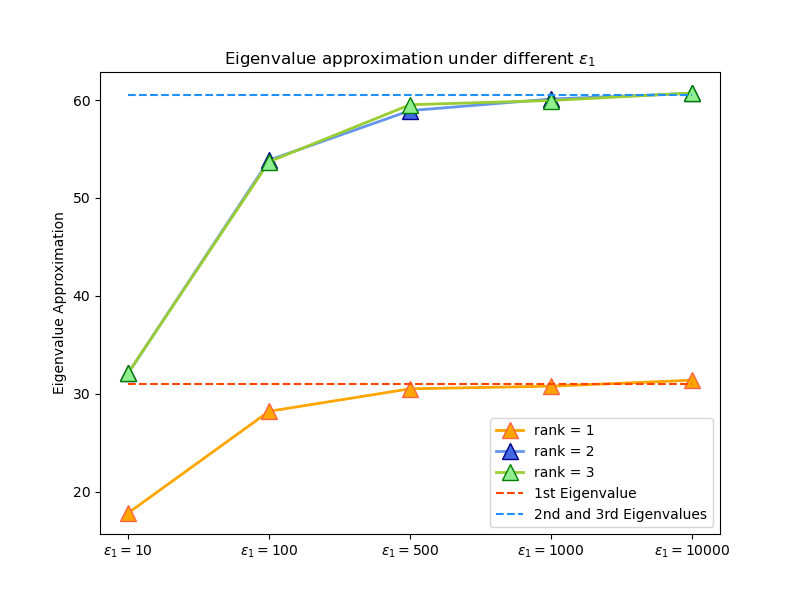
\includegraphics[width=0.7\textwidth]{figures1/EigFig2023/under-different-lambda1.png}
%     \caption{Eigenvalue approximation under different $\varepsilon_1$}\label{lambda1}
%     \label{fig:lambda1}
% \end{figure}

% 首先，我们选取不同的 $\varepsilon_1$ 值并使用 Deep Ritz 方法进行求解。所得结果展示于图 \ref{fig:lambda1}。定理 \ref{mainthm} 指出，随着 $\varepsilon_1$ 的增加，计算得到的特征值将趋近于真实值，实验结果验证了这一观察结论。

% 接下来，我们将讨论 $\varepsilon_2$ 对解的影响。我们选取了满足以下条件的 $\varepsilon_2$ 值：小于 $2\lambda_1$，略大于 $2\lambda_1$ 但小于 $2\lambda_2$ 和 $2\lambda_3$，略大于 $2\lambda_2$ 和 $2\lambda_3$，以及显著大于 $2\lambda_2$ 和 $2\lambda_3$。相关结果呈现于图 \ref{fig:lambda2}。

% 根据定理 \ref{mainthm}，当 $\varepsilon_2$ 大于 $2\lambda_k$ 时，第 $k$ 个特征值是可以被计算出来的。实验结果也验证了这一论述。当 $\varepsilon_2=10<2\lambda_1$ 时，算法无法计算出任何特征值。当 $2\lambda_1<\varepsilon_2=62<2\lambda_2$ 时，第一个特征值能够被较好地计算出来，但无法收敛至第二个特征值。当 $\varepsilon_2>2\lambda_2$ 时，所有对应的特征值均可被准确计算。

% \begin{figure}[htbp]
%     \centering
%     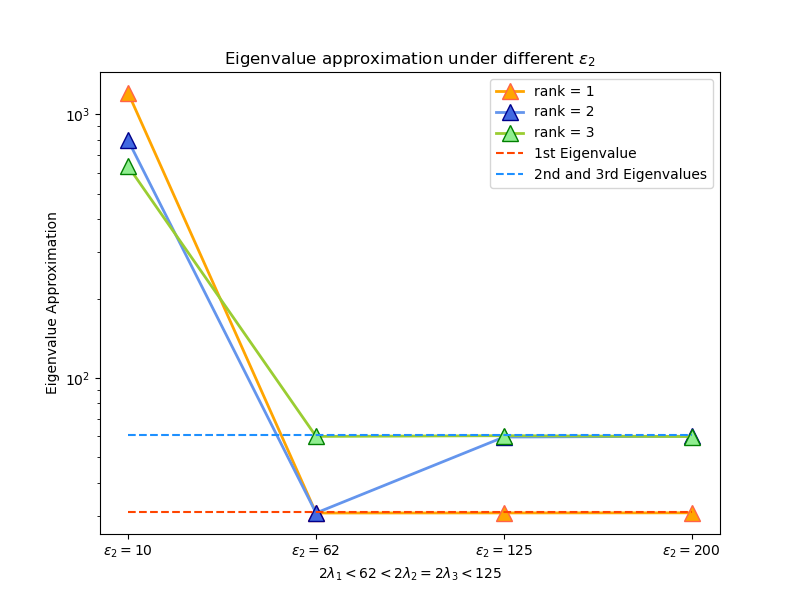
\includegraphics[width=0.6\textwidth]{figures1/EigFig2023/under-different-lambda2.png}
%     \caption{Eigenvalue approximation under different $\varepsilon_2$}
%     \label{fig:lambda2}
% \end{figure}

% 值得注意的是，当 $\varepsilon_2=62$ 时，第三个特征值似乎已被正确计算，这可能令人费解。为了阐明这一点，我们需要借助近似特征函数的热力图，如图 \ref{fig:heatmap} 所示。众所周知，在二维情形下，第二和第三个特征值在数值上相等，但对应于两个正交的特征函数。通过特征函数的热力图可以观察到，在计算第二个特征值时，由于 $\varepsilon_2$ 取值较小，解退化为了第一个特征函数。然而，在计算第三个特征值时，损失函数包含了两个与第一个特征值相关的正交项。因此，这等价于使用 $2\varepsilon_2$ 计算第二个特征值。这一观察结果与我们的理论分析保持一致。
% \begin{figure}[htbp]
%     \centering
%     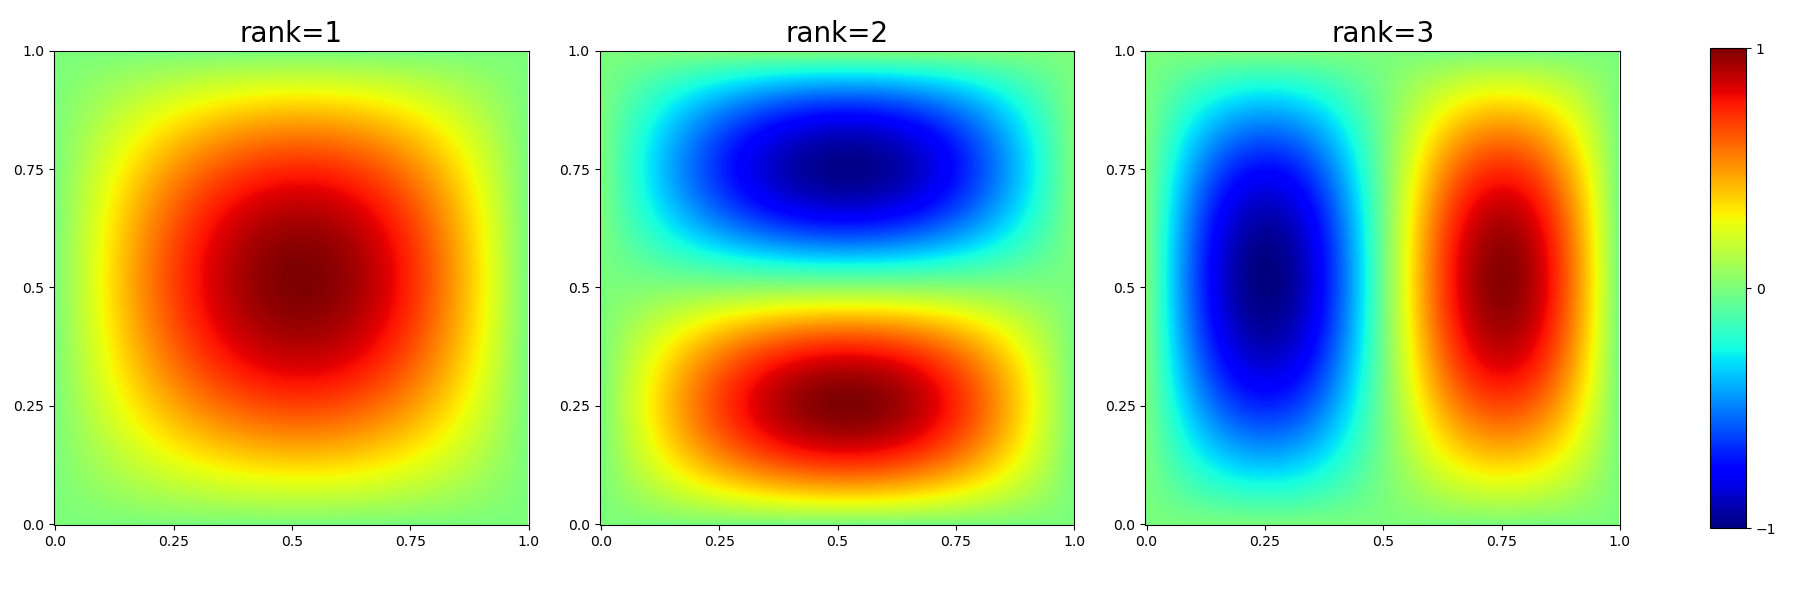
\includegraphics[width=0.8\textwidth]{figures1/EigFig2023/heat-map-reference.png}
%     \caption{Eigenfunction reference}
% \end{figure}
% \begin{figure}[htbp]
%     \centering
%     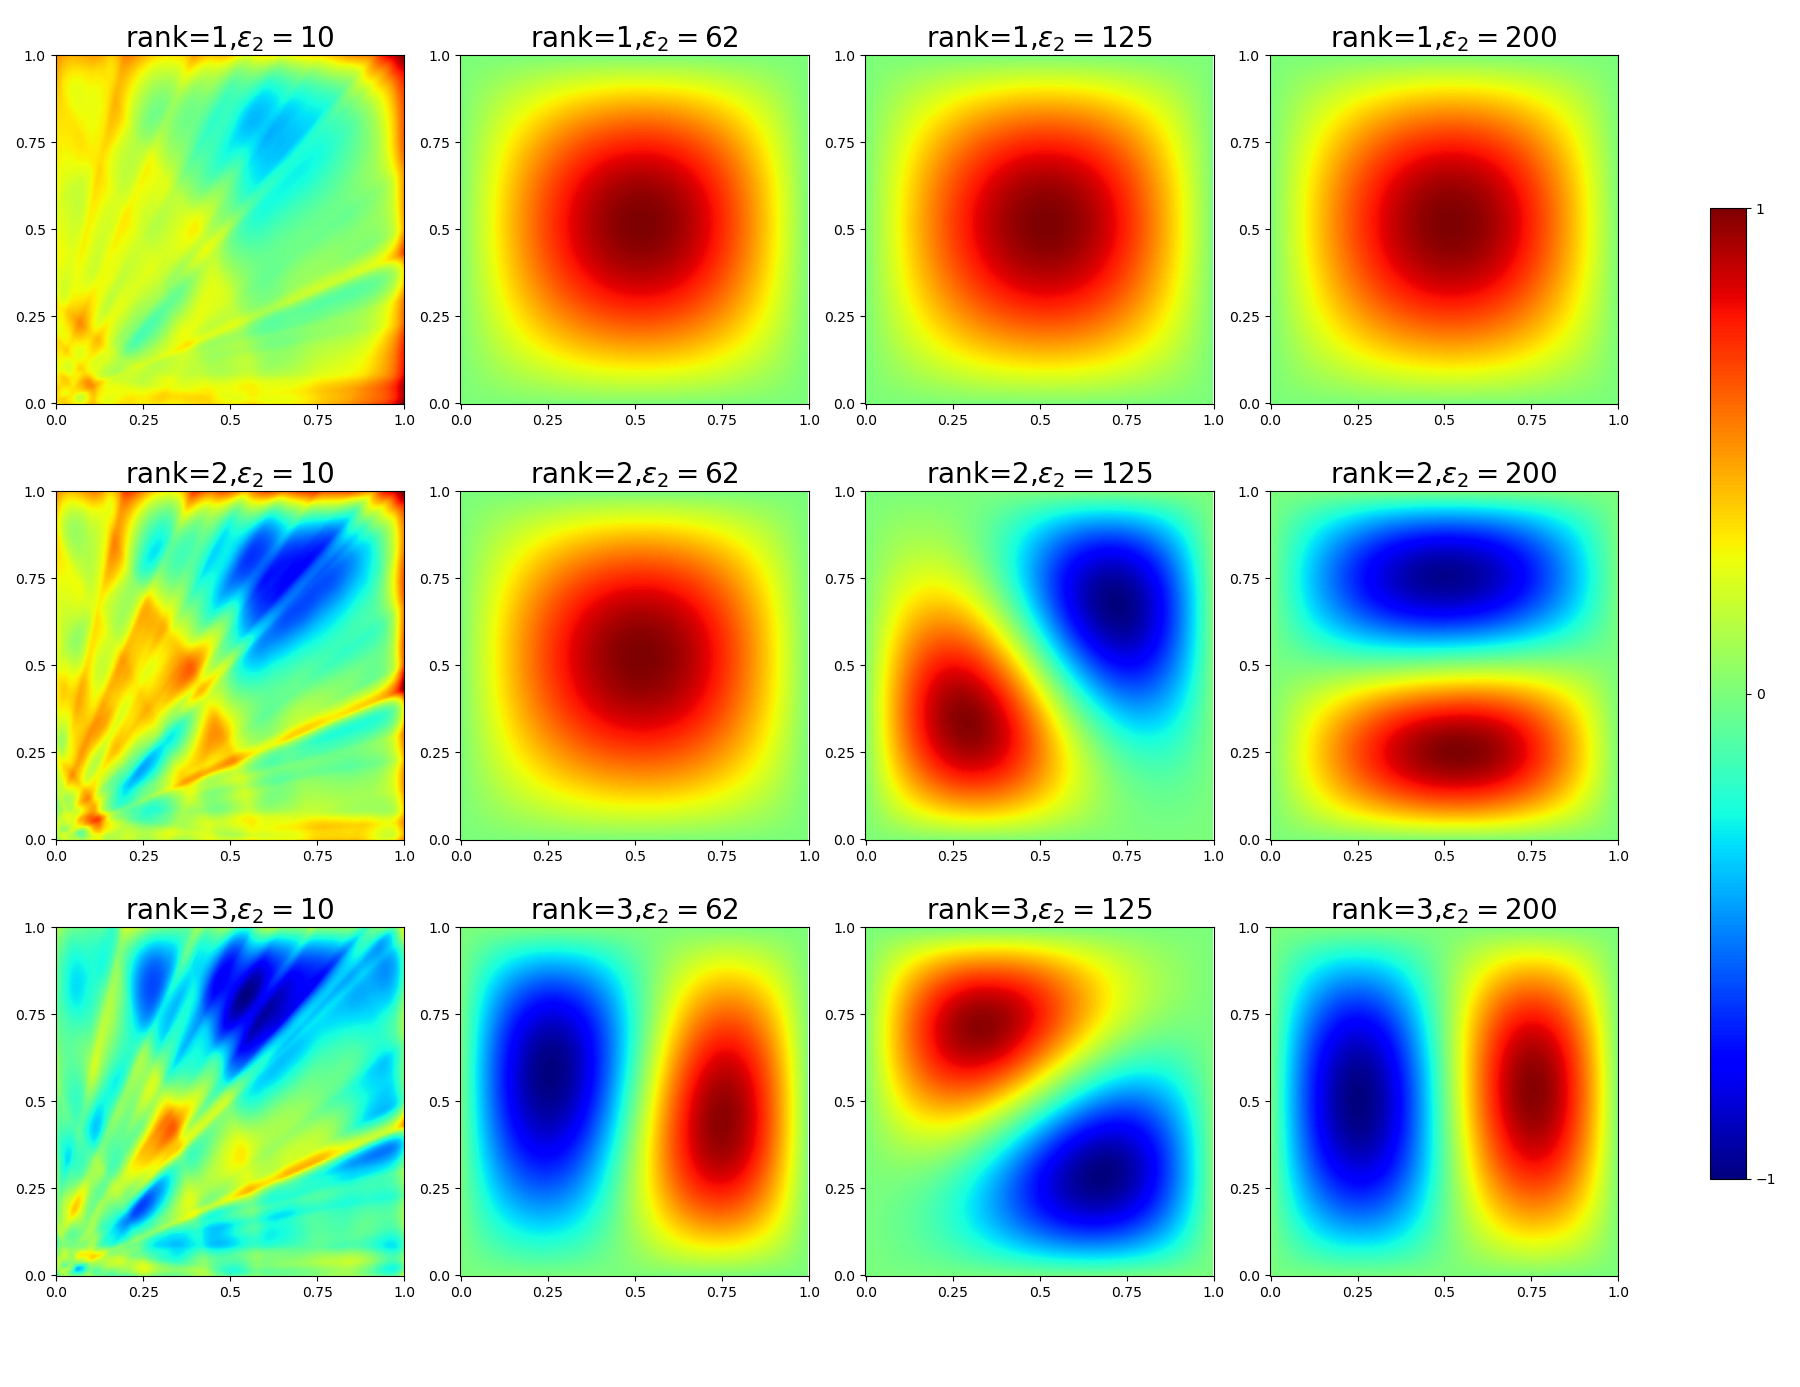
\includegraphics[width=0.8\textwidth]{figures1/EigFig2023/heat-map.png}
%     \caption{Heatmap for eigenfunction approximation for $\varepsilon_2=125$ and $\varepsilon_2=200$. }\label{fig:heatmap}
% \end{figure}

% 最后，我们考察了网络宽度和采样大小对解的影响。正如预期的那样，通过增加网络宽度和扩大采样规模，我们通常能够获得更精确的解

% \begin{figure}[htbp]
%     \centering
%     % 第一个子图
%     \begin{subfigure}{0.45\textwidth}
%         \centering
%         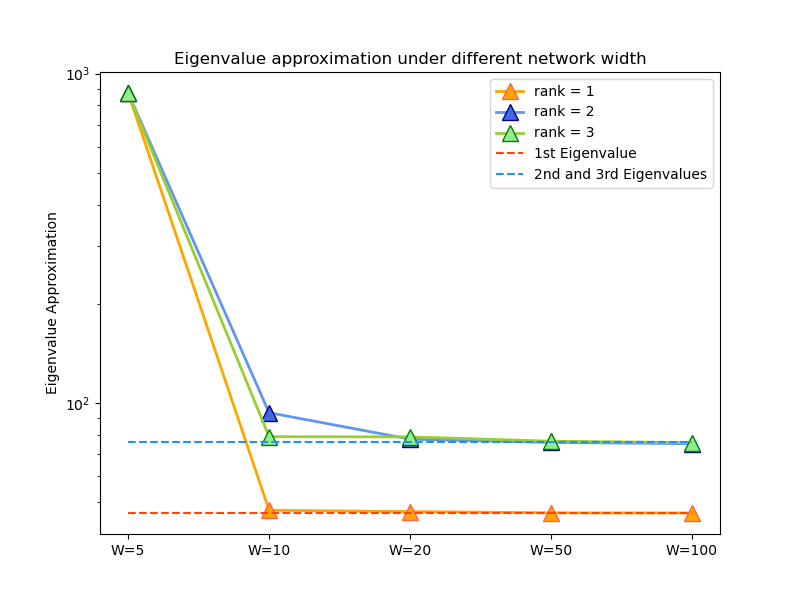
\includegraphics[width=\linewidth]{figures1/EigFig2023/under-different-width.png}
%         \caption{不同 $\mathcal{W}$ 下的特征值逼近}
%         \label{fig:width}
%     \end{subfigure}
%     \hfill % 关键：把两图撑开到两边
%     % 第二个子图
%     \begin{subfigure}{0.45\textwidth}
%         \centering
%         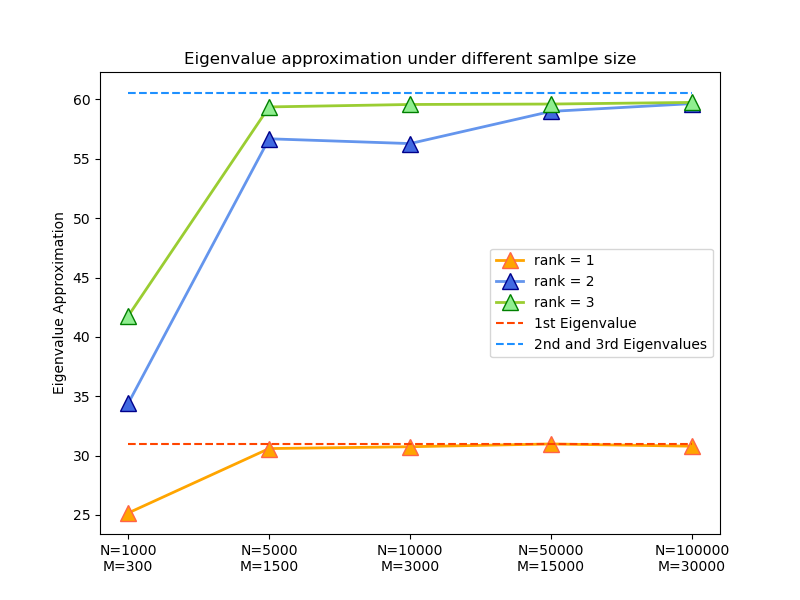
\includegraphics[width=\linewidth]{figures1/EigFig2023/under-different-sample.png}
%         \caption{不同样本量下的特征值逼近}
%         \label{fig:sample}
%     \end{subfigure}
    
%     \caption{网络宽度和采样大小的影响}
%     \label{fig:main}
% \end{figure}

% \subsection{立方体区域上的拉普拉斯特征值问题}\label{sec:10dcube}
% 在本节及下一节中，我们在 Eq.~\eqref{eq:conloss} 中选取了不同的函数 $w(x)$，包括常用的函数，如指数函数 $(w(x)=\exp(-\pi x))$ 和平方函数 $(w(x)=x^2)$。此外，我们探索了不同的区域，包括 10 维立方体和 10 维球体。在这些区域上，依赖于空间离散化的传统数值算法（如有限元法和有限差分法）一直无法提供令人满意的结果。实验的参数设置如下：

% \begin{table}[htbp]
% \centering
% \begin{tabular}{l|ccc}
% \toprule
% {\heiti 参数} & {\heiti 平方势} & \multicolumn{1}{p{2.2cm}}{{\heiti 指数势}} & \multicolumn{1}{p{3.2cm}}{{\heiti 简谐振子}}\\
% \midrule
% 区域 & $[0,1]^{10}$ &  $[0,1]^{10}$ & $\mathbb{R}^{10}$ 中的单位球 \\
% 学习率 & 0.001& 0.001& 0.001\\
% 训练轮数 (Epoch)& 100000& 100000& 50000\\
% $\varepsilon_1/\varepsilon_2$& 2000/1000&  2000/500& 2000/600\\
% 宽度/深度
% & 150/4 & 150/4 & 60/4 \\
% 样本量 ($\Omega$)& 200000& 200000& 200000\\
% 样本量 ($\partial\Omega$)& 80000& 80000& 80000\\
% \bottomrule
% \end{tabular}
% \caption{第 \ref{sec:10dcube} 节和第 \ref{sec:10dball} 节中的参数设置。}
% \end{table}

% \begin{figure}[htbp]
%     \centering
    
%     % --- 第一行 ---
%     % 创建一个子图容器，宽度约为页面宽度的一半
%     \begin{subfigure}{0.48\linewidth}
%         \centering
%         % 图片宽度占满当前子图容器
%         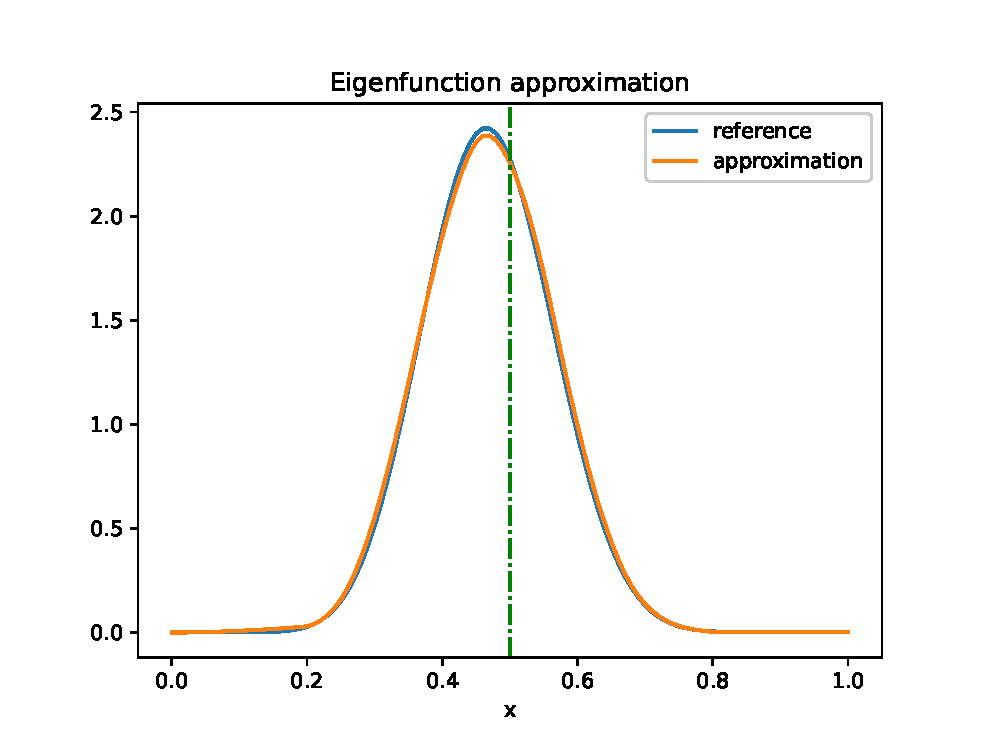
\includegraphics[width=\linewidth]{figures1/1square/unn_rank1.eps}
%         \caption{方形势下的 $\widehat{\xi}_{\phi 1}$}
%         \label{fig:sq1}
%     \end{subfigure}
%     \hfill % 弹性填充，将两个子图推向两侧
%     \begin{subfigure}{0.48\linewidth}
%         \centering
%         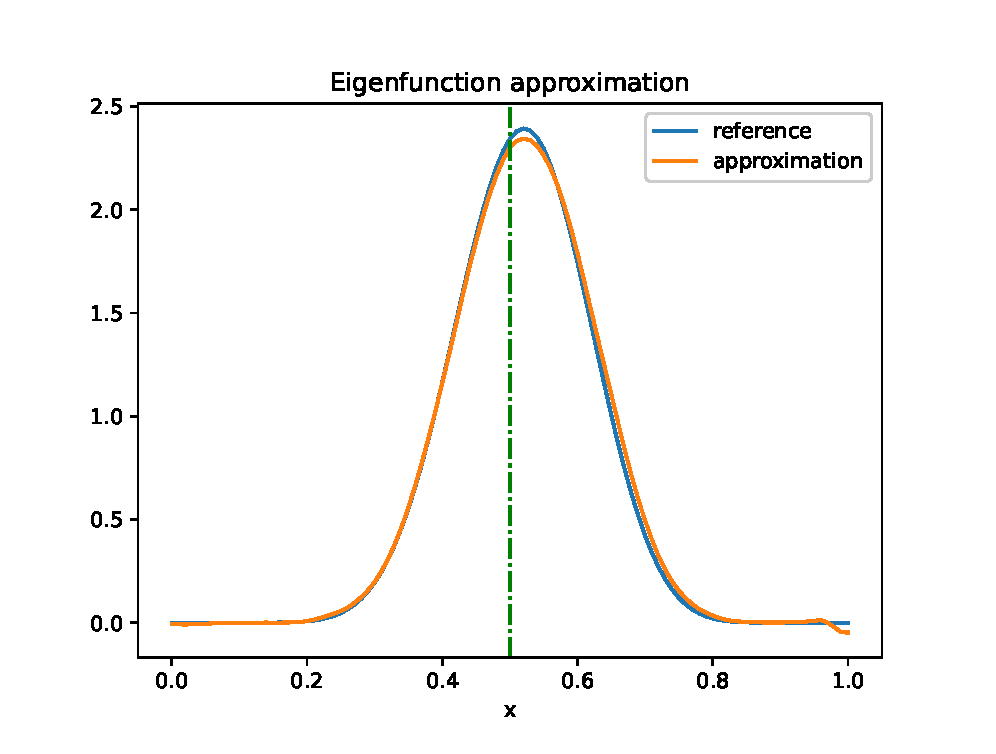
\includegraphics[width=\linewidth]{figures1/1expc/unn_rank1.eps}
%         \caption{指数势下的 $\widehat{\xi}_{\phi 1}$}
%         \label{fig:exp1}
%     \end{subfigure}
    
%     \vspace{1em} % 增加行间距
    
%     % --- 第二行 ---
%     \begin{subfigure}{0.48\linewidth}
%         \centering
%         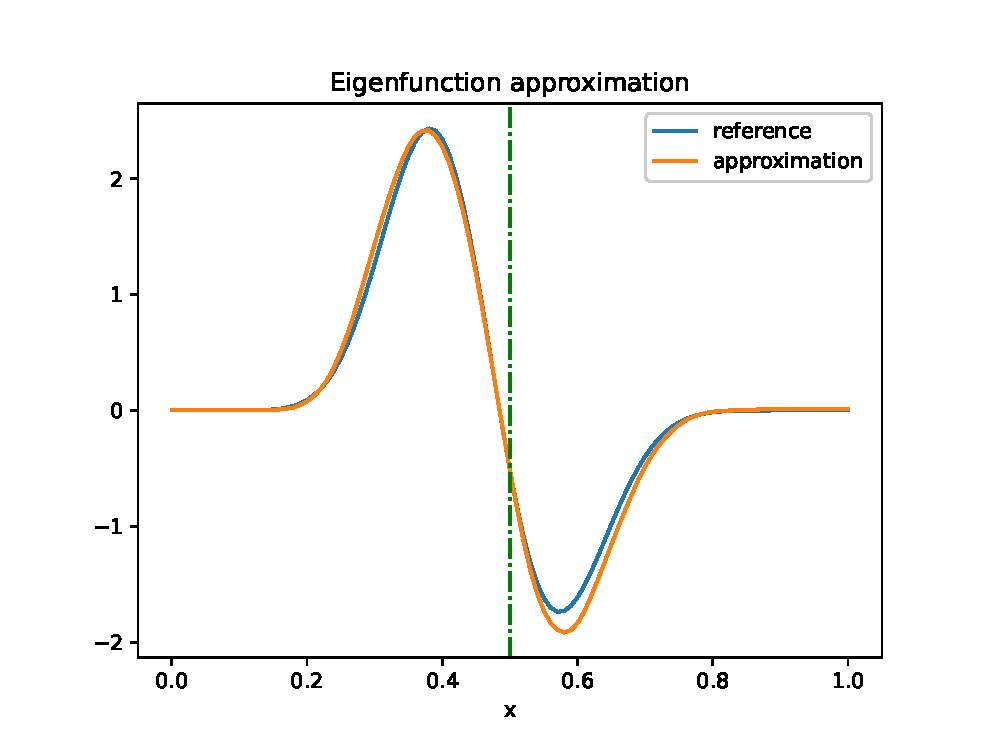
\includegraphics[width=\linewidth]{figures1/2square/unn_rank2.eps}
%         \caption{方形势下的 $\widehat{\xi}_{\phi 2}$}
%         \label{fig:sq2}
%     \end{subfigure}
%     \hfill
%     \begin{subfigure}{0.48\linewidth}
%         \centering
%         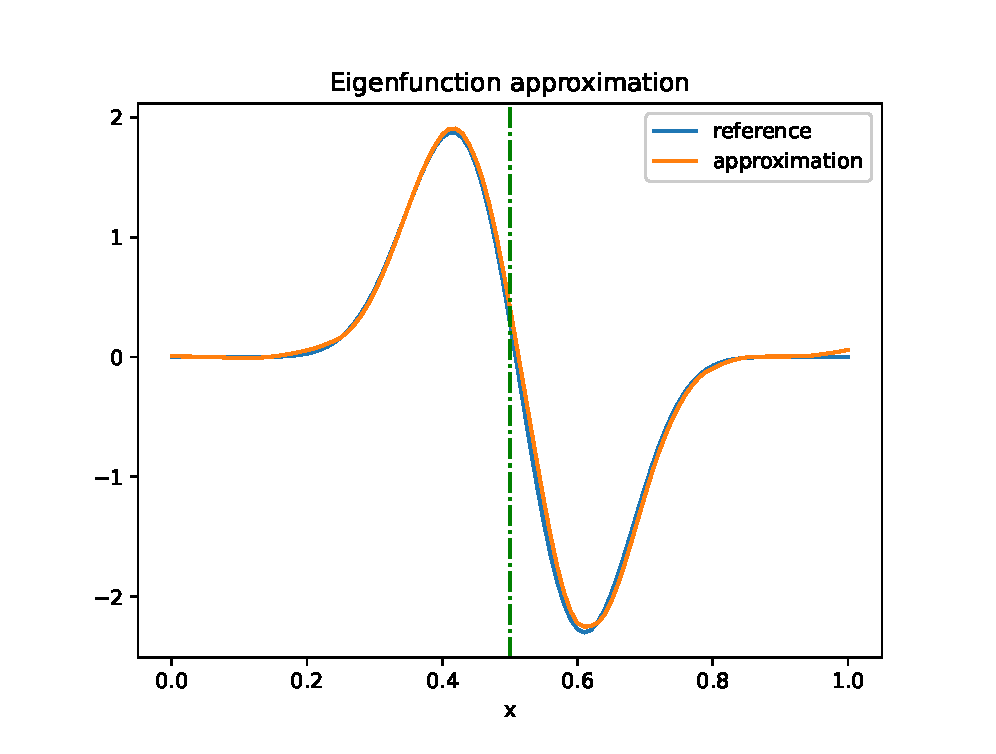
\includegraphics[width=\linewidth]{figures1/2expc/unn_rank2.eps}
%         \caption{指数势下的 $\widehat{\xi}_{\phi 2}$}
%         \label{fig:exp2}
%     \end{subfigure}
    
%     \vspace{1em} % 增加行间距
    
%     % --- 第三行 ---
%     \begin{subfigure}{0.48\linewidth}
%         \centering
%         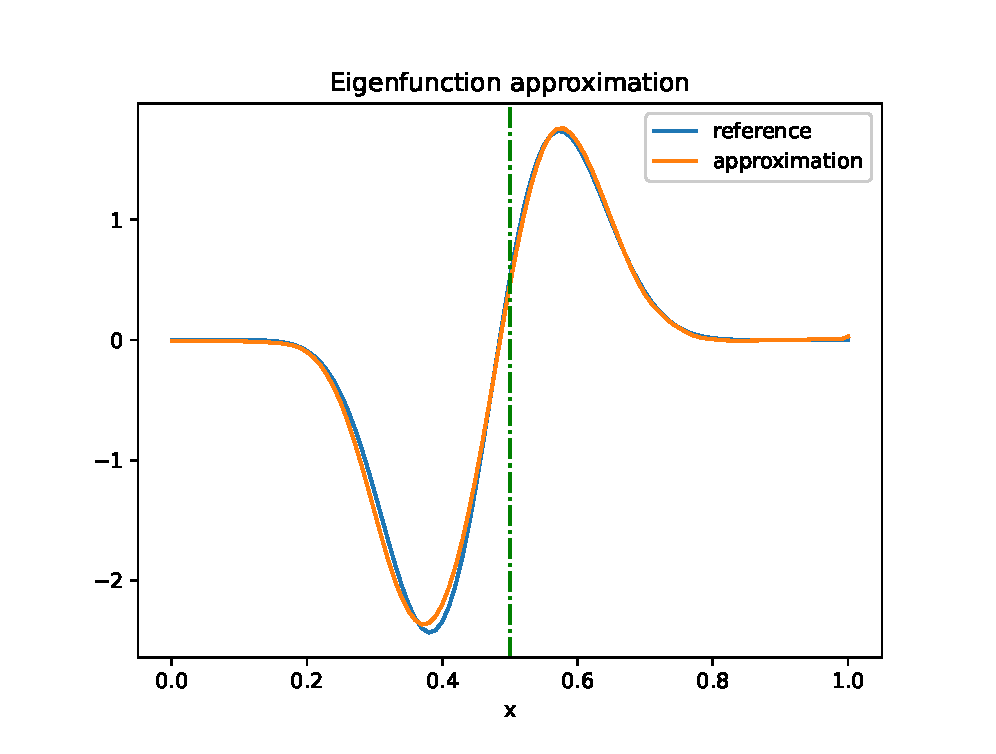
\includegraphics[width=\linewidth]{figures1/3square/unn_rank3.eps}
%         \caption{方形势下的 $\widehat{\xi}_{\phi 3}$}
%         \label{fig:sq3}
%     \end{subfigure}
%     \hfill
%     \begin{subfigure}{0.48\linewidth}
%         \centering
%         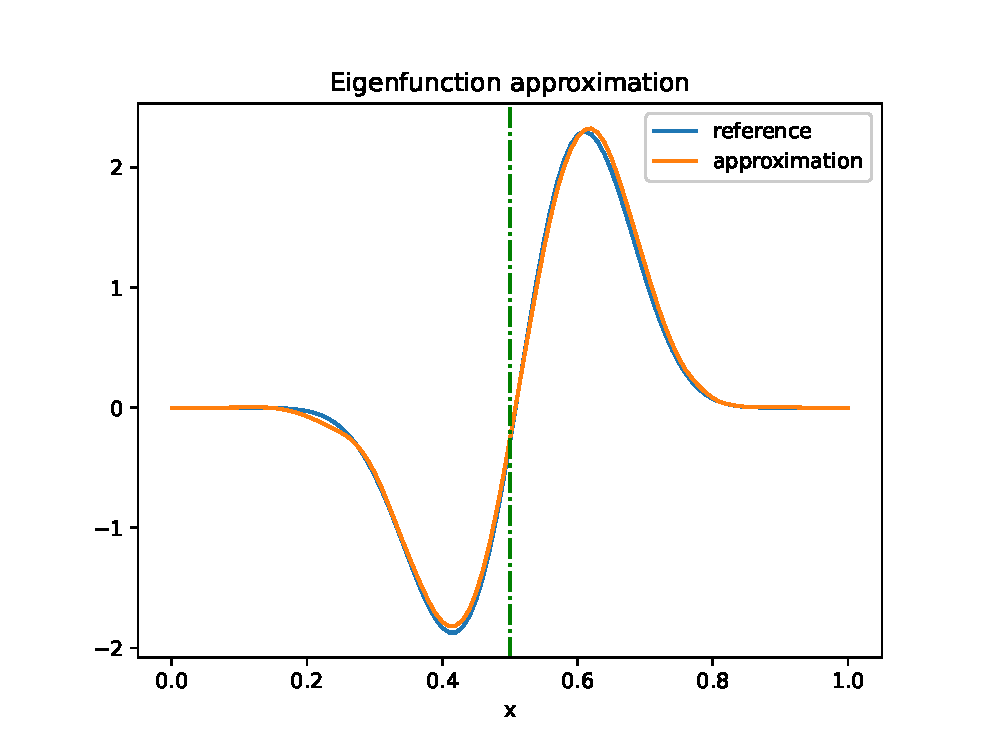
\includegraphics[width=\linewidth]{figures1/3expc/unn_rank3.eps}
%         \caption{指数势下的 $\widehat{\xi}_{\phi 3}$}
%         \label{fig:exp3}
%     \end{subfigure}
    
%     % 总标题
%     \caption{方形势和指数势在立方体区域对角线上的本征函数。}
%     \label{fig1}
% \end{figure}

% \begin{figure}[htbp]
%     \centering
    
%     % --- 第一行：lambda_1 ---
%     \begin{subfigure}{0.48\textwidth}
%         \centering
%         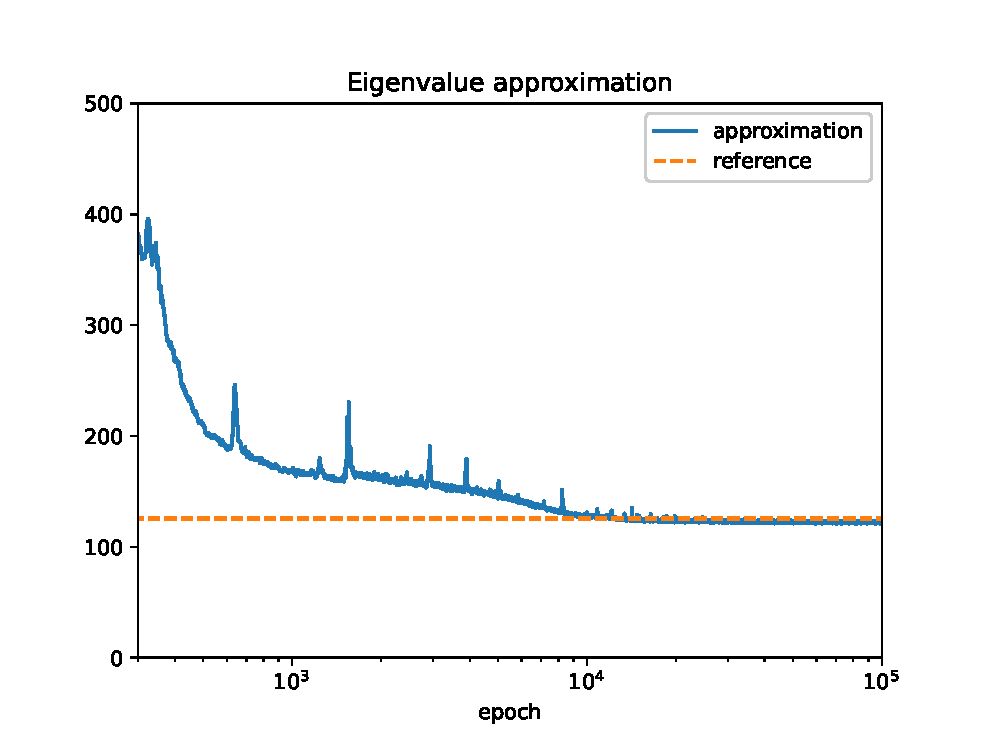
\includegraphics[width=\linewidth]{figures1/1square/eigenvalue_rank1.eps}
%         \caption{方势的 $\lambda_{1}$}
%     \end{subfigure}
%     \hfill
%     \begin{subfigure}{0.48\textwidth}
%         \centering
%         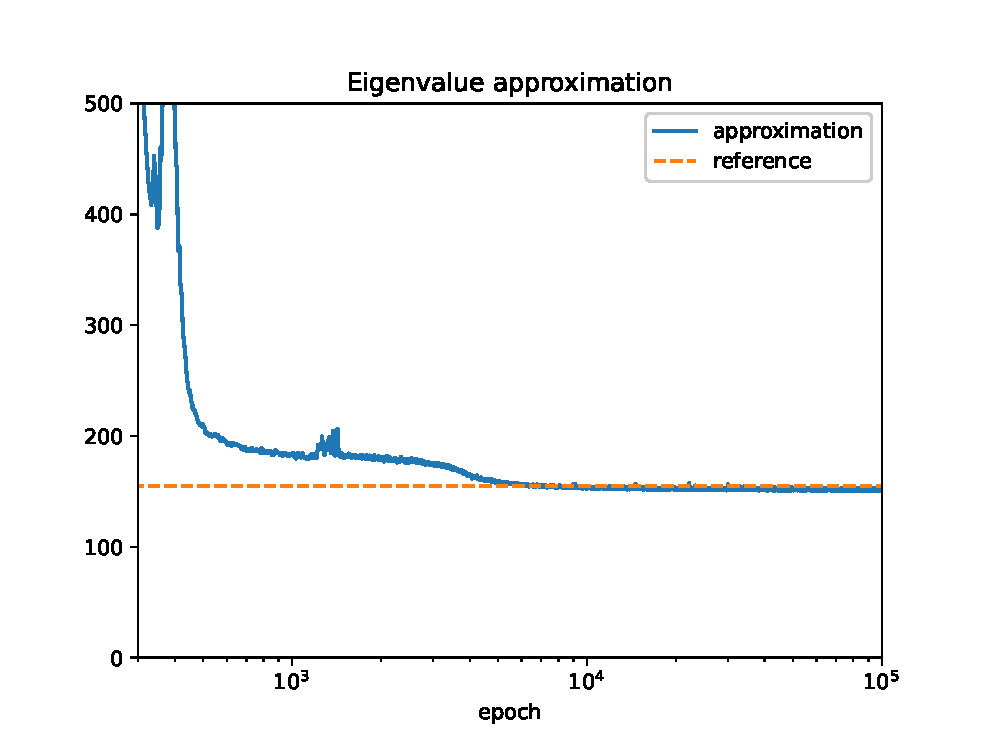
\includegraphics[width=\linewidth]{figures1/1expc/eigenvalue_rank1.eps}
%         \caption{指数势的 $\lambda_{1}$}
%     \end{subfigure}
    
%     \vspace{1em} % 增加行间距
    
%     % --- 第二行：lambda_2 ---
%     \begin{subfigure}{0.48\textwidth}
%         \centering
%         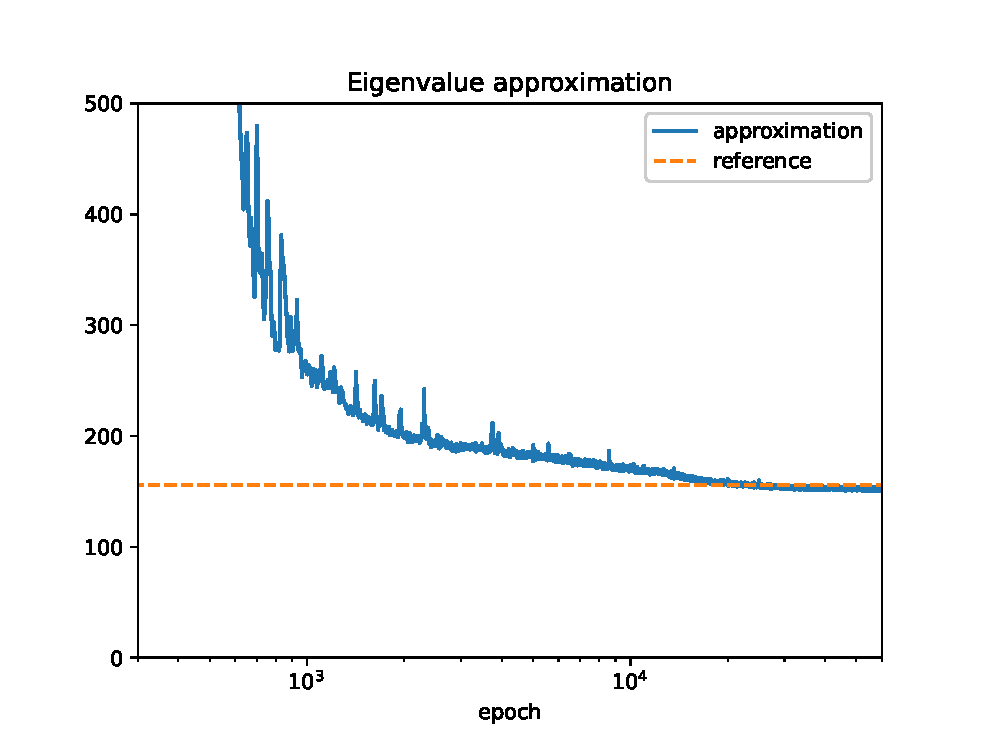
\includegraphics[width=\linewidth]{figures1/2square/eigenvalue_rank2.eps}
%         \caption{方势的 $\lambda_{2}$}
%     \end{subfigure}
%     \hfill
%     \begin{subfigure}{0.48\textwidth}
%         \centering
%         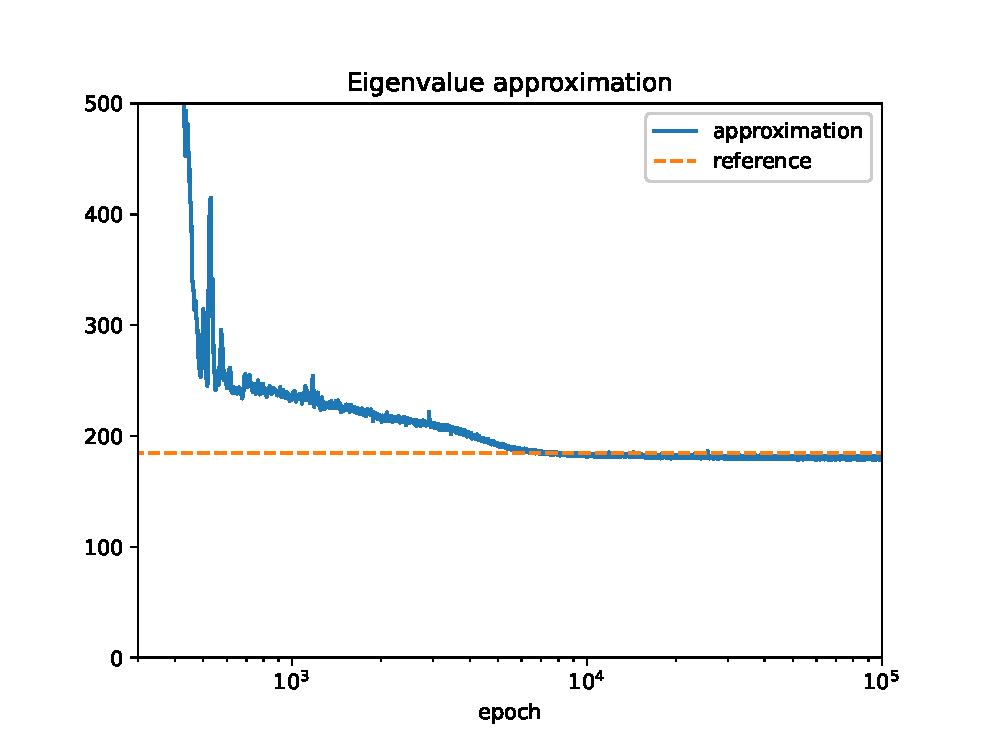
\includegraphics[width=\linewidth]{figures1/2expc/eigenvalue_rank2.eps}
%         \caption{指数势的 $\lambda_{2}$}
%     \end{subfigure}
    
%     \vspace{1em} % 增加行间距
    
%     % --- 第三行：lambda_3 ---
%     \begin{subfigure}{0.48\textwidth}
%         \centering
%         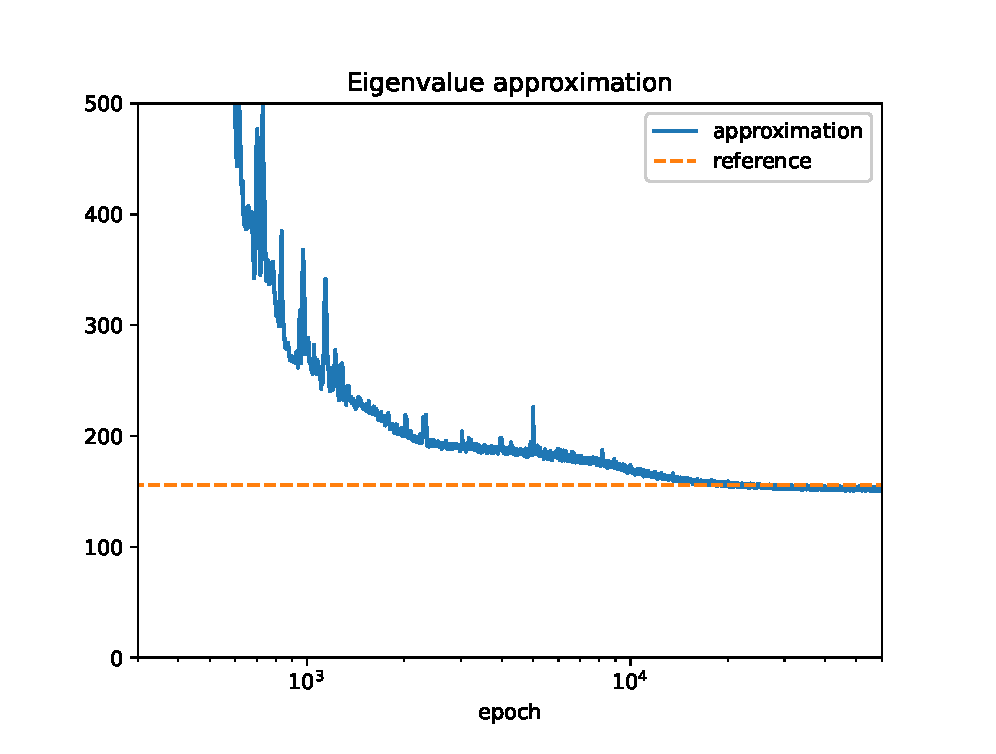
\includegraphics[width=\linewidth]{figures1/3square/eigenvalue_rank3.eps}
%         \caption{方势的 $\lambda_{3}$}
%     \end{subfigure}
%     \hfill
%     \begin{subfigure}{0.48\textwidth}
%         \centering
%         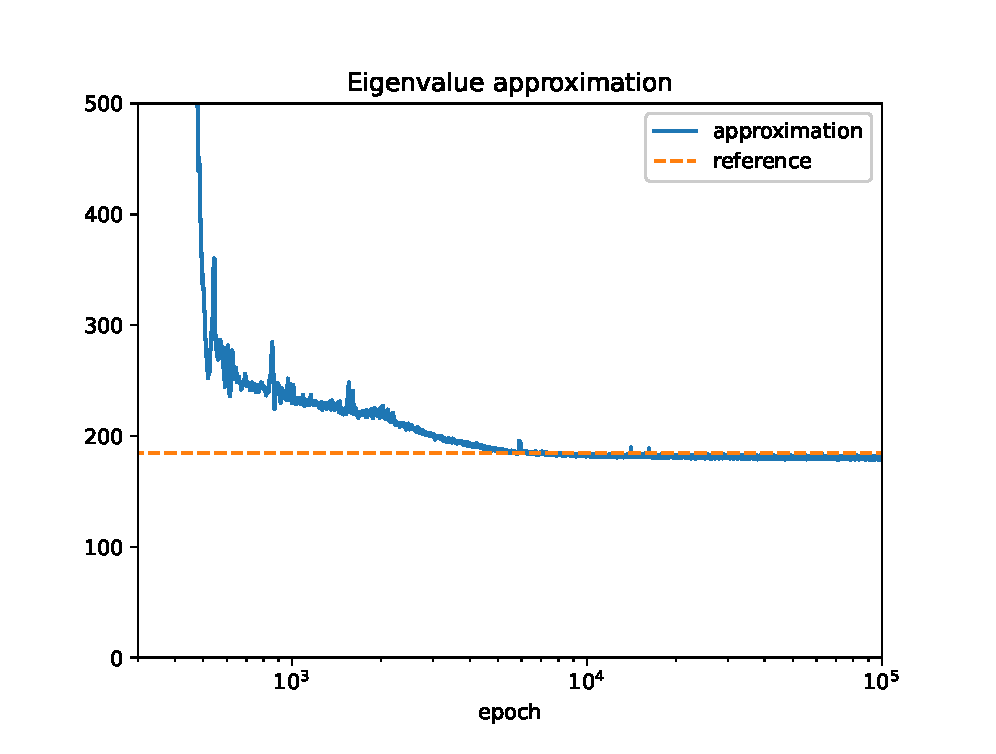
\includegraphics[width=\linewidth]{figures1/3expc/eigenvalue_rank3.eps}
%         \caption{指数势的 $\lambda_{3}$}
%     \end{subfigure}
    
%     % 总标题
%     % 这一段红字依赖 \usepackage{xcolor}
%     \caption{训练过程中方势与指数势的特征值逼近情况。}
%     \label{fig2}
% \end{figure}

% 如图 \ref{fig1} 和 \ref{fig2} 所示，所有估计的特征值和特征函数均与其各自的精确值非常接近。计算得到的特征值小于精确值，这与定理 \ref{mainthm} 的结论相符。

% \subsection{单位球上的拉普拉斯特征值问题}\label{sec:10dball}
% 在本节中，我们求解 $\mathbb{R}^{10}$ 和 $\mathbb{R}^{20}$ 空间中单位球的特征值问题。与上述情形不同，在此情形下，由于受到无限深势阱的束缚，所有的 $x_{i}$ 不再是独立运动的：
% \begin{equation*}
% V(x)=\left\{
% \begin{array}{ll}
% 0&|x|<1,\\
% +\infty&|x|\geq 1.
% \end{array}\right.
% \end{equation*}
% 在此情形下，第一特征值 $\lambda_{1}$ 是四阶贝塞尔函数的第一根，而第二特征值 $\lambda_{2}$ 是五阶贝塞尔函数的第一根。所有对应的特征函数可表示为：
% \begin{equation*}
% \xi_{k}(x)\in\mathop{span}\left\{ \frac{1}{\left(\lambda_{k}|x|\right)^{4+l}}J_{4+l}(\lambda_{k}|x|)P_{l}(x),\quad l=0,1,2,\cdots, \quad k=1,2,3,\cdots .\right\},
% \end{equation*}
% 其中 $P_{l}(x)$ 是一个 $l$ 次齐次多项式。

% \begin{figure}[htbp]
%     \centering
    
%     % --- 第一行 (Rank 1) ---
%     \begin{subfigure}{0.48\textwidth}
%         \centering
%         % 使用 \linewidth 让图片自动适应子图容器的宽度
%         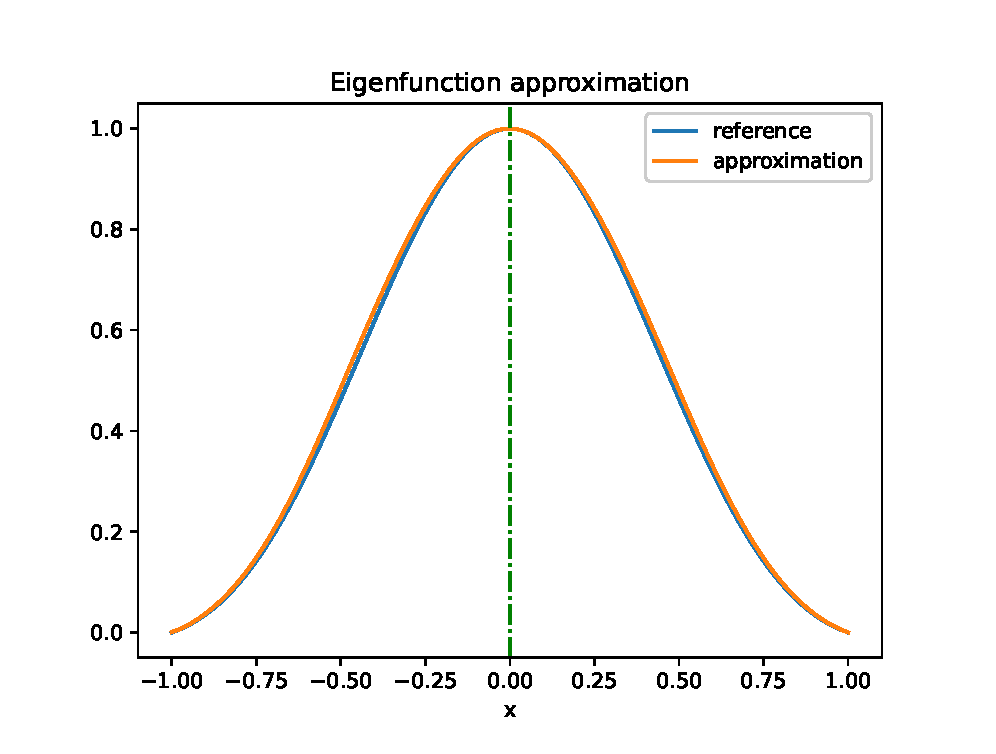
\includegraphics[width=\linewidth]{figures1/ball/ball_unn_rank1.eps}
%         \caption{单位球上的 $\widehat{\xi}_{\phi 1}$}
%     \end{subfigure}
%     \hfill % 左右推开
%     \begin{subfigure}{0.48\textwidth}
%         \centering
%         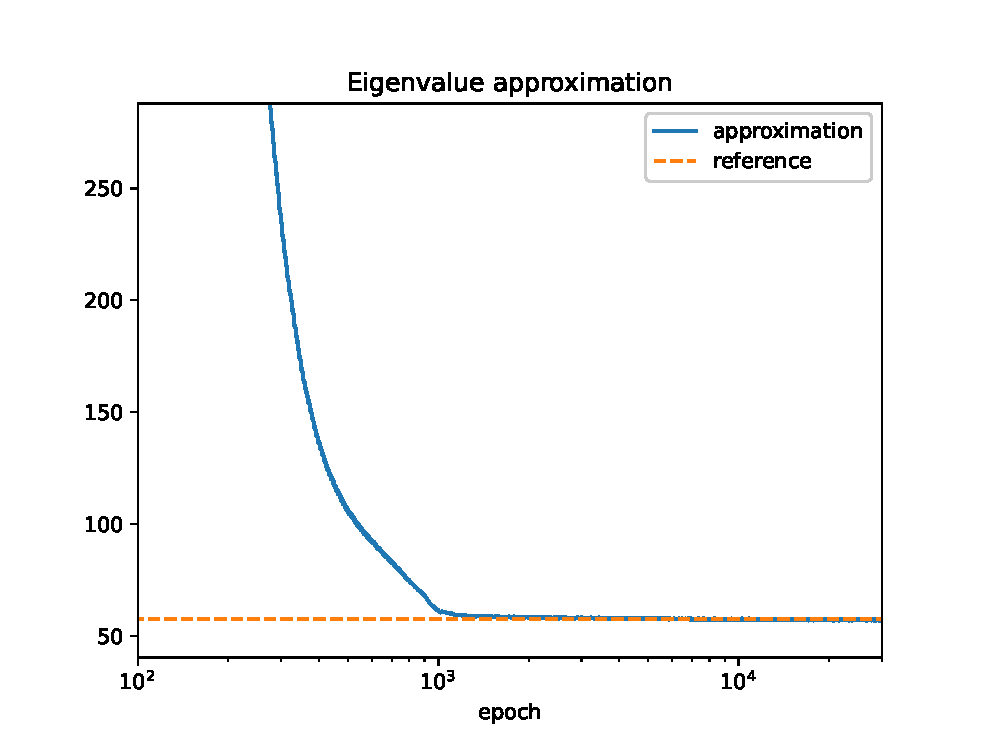
\includegraphics[width=\linewidth]{figures1/ball/ball_eigenvalue_rank1.eps}
%         \caption{单位球上的 $\lambda_{1}$}
%     \end{subfigure}
    
%     \vspace{0.5em} % 行间距，防止上下两行太挤
    
%     % --- 第二行 (Rank 2) ---
%     \begin{subfigure}{0.48\textwidth}
%         \centering
%         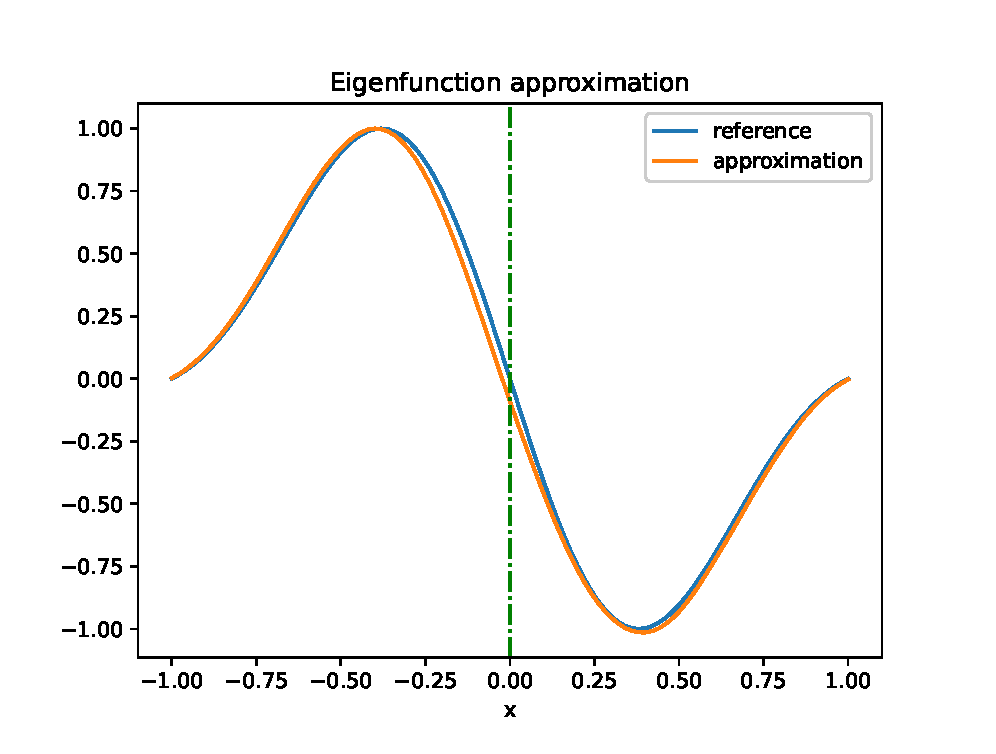
\includegraphics[width=\linewidth]{figures1/ball/ball_unn_rank2.eps}
%         \caption{单位球上的 $\widehat{\xi}_{\phi 2}$}
%     \end{subfigure}
%     \hfill
%     \begin{subfigure}{0.48\textwidth}
%         \centering
%         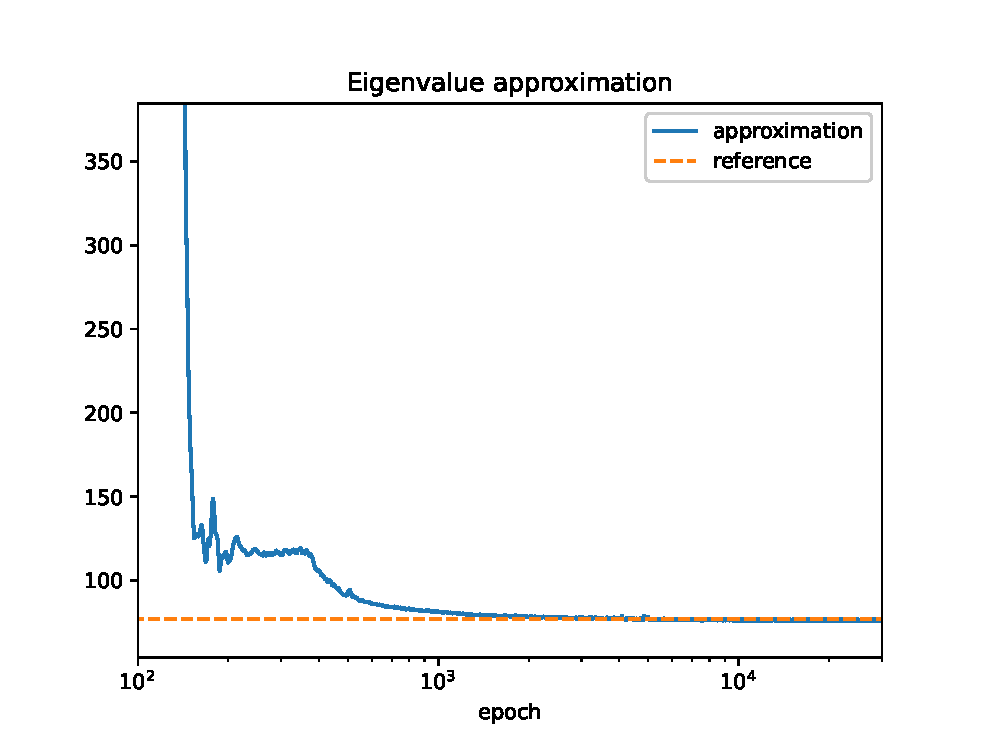
\includegraphics[width=\linewidth]{figures1/ball/ball_eigenvalue_rank2.eps}
%         \caption{单位球上的 $\lambda_{2}$}
%     \end{subfigure}
    
%     \vspace{0.5em} % 行间距
    
%     % --- 第三行 (Rank 3) ---
%     \begin{subfigure}{0.48\textwidth}
%         \centering
%         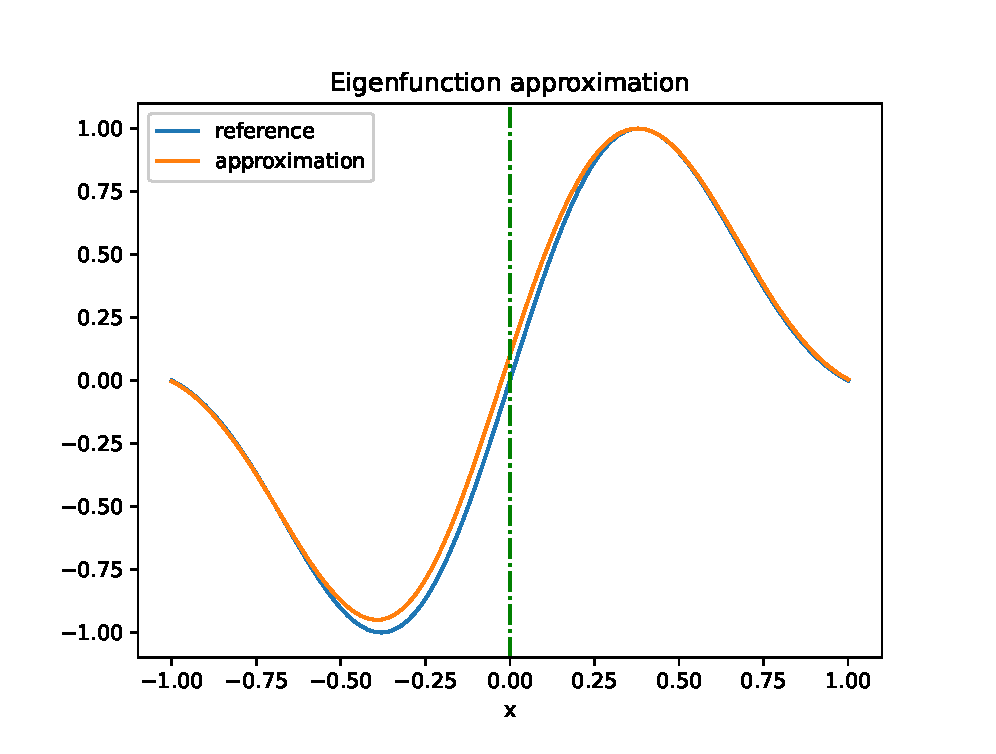
\includegraphics[width=\linewidth]{figures1/ball/ball_unn_rank3.eps}
%         \caption{单位球上的 $\widehat{\xi}_{\phi 3}$}
%     \end{subfigure}
%     \hfill
%     \begin{subfigure}{0.48\textwidth}
%         \centering
%         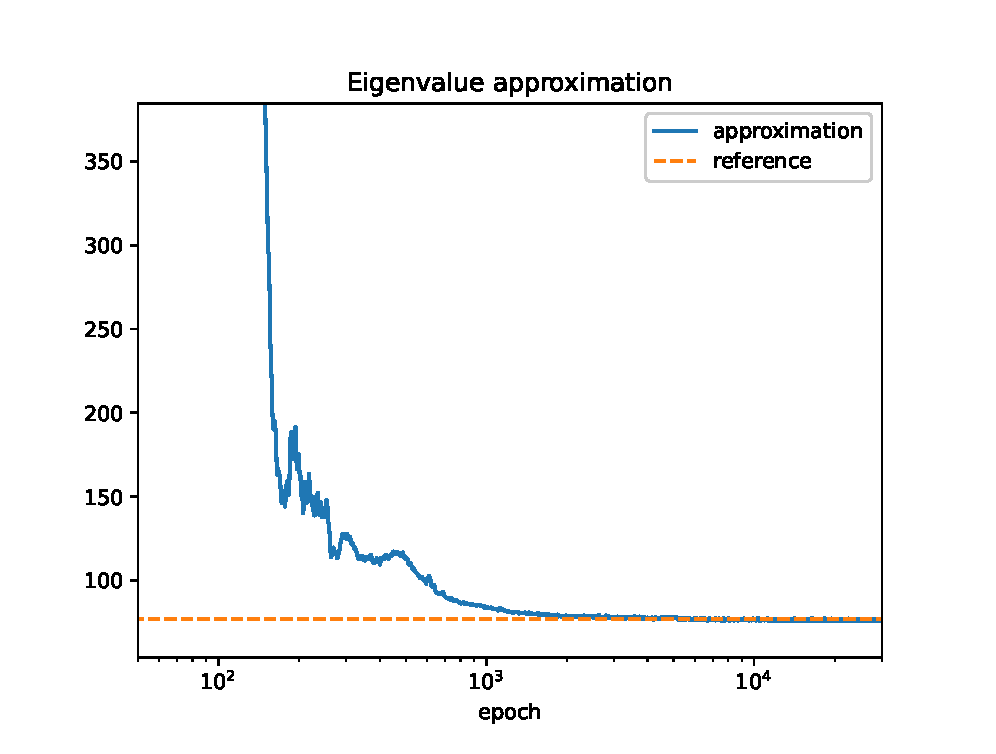
\includegraphics[width=\linewidth]{figures1/ball/ball_eigenvalue_rank3.eps}
%         \caption{单位球上的 $\lambda_{3}$}
%     \end{subfigure}
    
%     % --- 总标题 ---
%     \caption{左图：对应于 10 维单位球对角线上的特征函数。右图：随训练轮数（epoch）变化的对应特征值演化。}
%     \label{fig3}
% \end{figure}

% 对于 $\mathbb{R}^{10}$，结果展示在图 \ref{fig3} 中，在此设置下，所提出的方法很好地估计了特征值和特征函数。

% 对于 $\mathbb{R}^{20}$ 的情形，使用蒙特卡洛方法计算积分面临挑战。具体而言，高维空间区域中的均匀采样会导致采样点在边界附近过度集中。为了克服这一挑战，常见的策略包括增加采样点数量以及实施更高效的采样技术。作为一种解决方案，我们采用了分层采样方法。该方法将单位球划分为两个不同的区域，记为 $B_{20}(0,1/2)$ 和 $B_{20}(0,1)/B_{20}(0,1/2)$。我们对每个区域分别计算蒙特卡洛积分，随后将所得数值进行加权求和。

% 这种采样方法确保了采样在一定程度上能够捕捉到区域内部的信息，从而提升了算法的性能。实验结果展示在附图 \ref{fig:20dball} 中。

% \begin{table}[h]
% \centering
% \begin{tabular}{l|c}
% \toprule
% {\heiti 参数} & {\heiti 简谐振子}\\
% \midrule
% 区域 & $\mathbb{R}^{20}$ 中的单位球\\
% 学习率 & 0.001\\
% 第 1 个特征值的训练轮数 & 100000\\
% 第 2、3 个特征值的训练轮数 & 200000\\
% $\varepsilon_1/\varepsilon_2$ & 5000/3000\\
% 宽度/深度 & 120/4\\
% 样本数量 ($B_{20}(0,0.5)$) & 50000\\
% 样本数量 ($B_{20}(0,1)/B_{20}(0,0.5)$) & 500000\\
% 样本数量 ($\partial B_{20}(0,1)$) & 200000\\
% \bottomrule
% \end{tabular}
% \caption{参数设置}
% \end{table}

% \begin{figure}[htbp]
%     \centering
    
%     % --- 第一行：Rank 1 ---
%     \begin{subfigure}{0.48\textwidth}
%         \centering
%         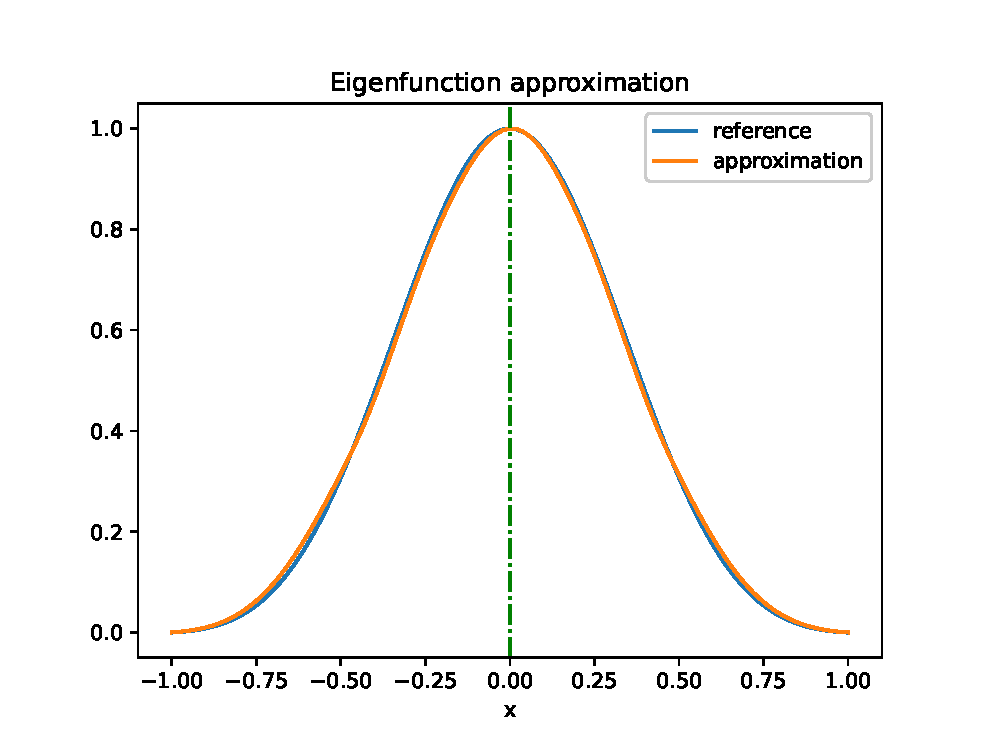
\includegraphics[width=\linewidth]{figures1/20d/unn_rank1.eps}
%         \caption{单位球上的 $\widehat{\xi}_{\phi 1}$}
%         \label{fig:xi_rank1}
%     \end{subfigure}
%     \hfill
%     \begin{subfigure}{0.48\textwidth}
%         \centering
%         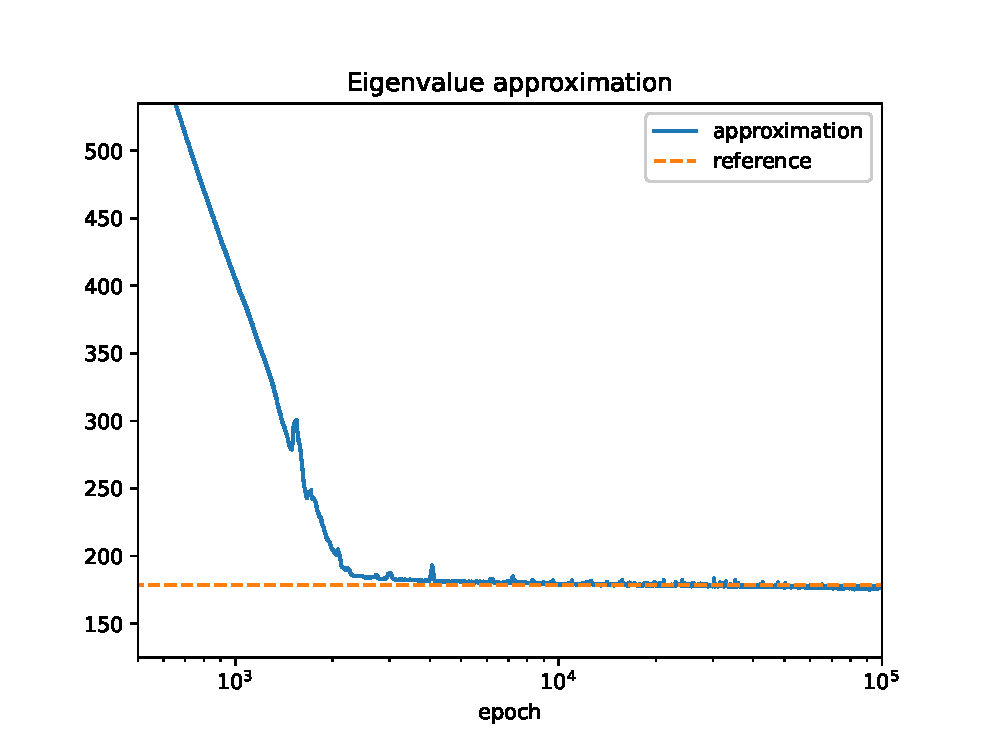
\includegraphics[width=\linewidth]{figures1/20d/eigenvalue_rank1.eps}
%         \caption{单位球上的 $\lambda_{1}$}
%         \label{fig:lambda_rank1}
%     \end{subfigure}
    
%     \vspace{1em} % 增加行间距
    
%     % --- 第二行：Rank 2 ---
%     \begin{subfigure}{0.48\textwidth}
%         \centering
%         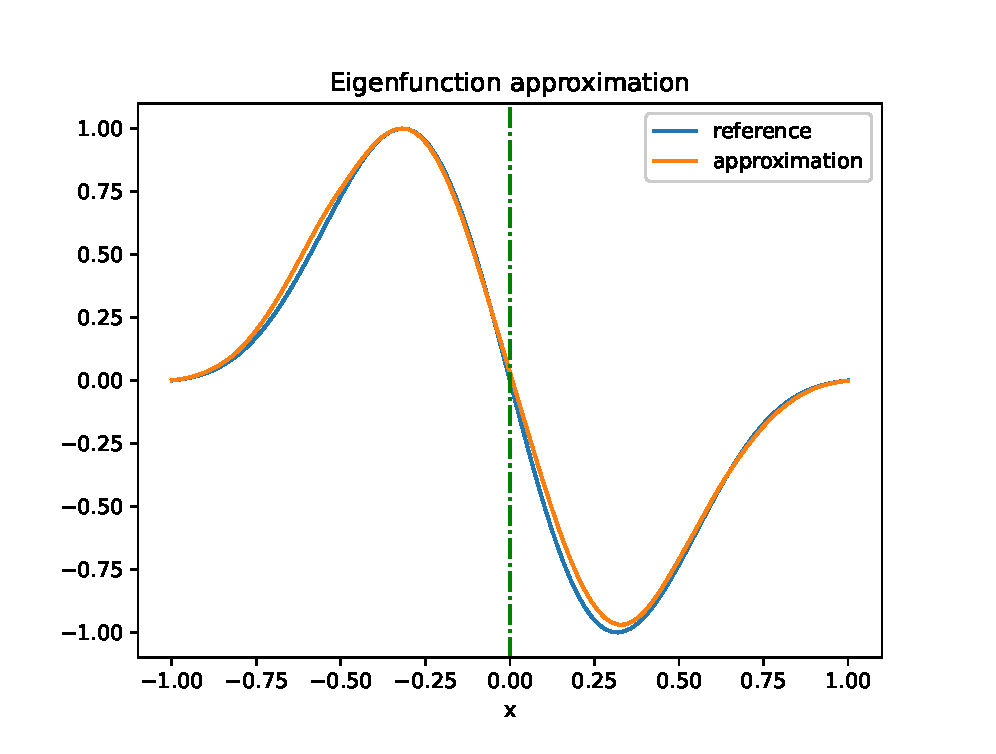
\includegraphics[width=\linewidth]{figures1/20d/unn_rank2.eps}
%         \caption{单位球上的 $\widehat{\xi}_{\phi 2}$}
%         \label{fig:xi_rank2}
%     \end{subfigure}
%     \hfill
%     \begin{subfigure}{0.48\textwidth}
%         \centering
%         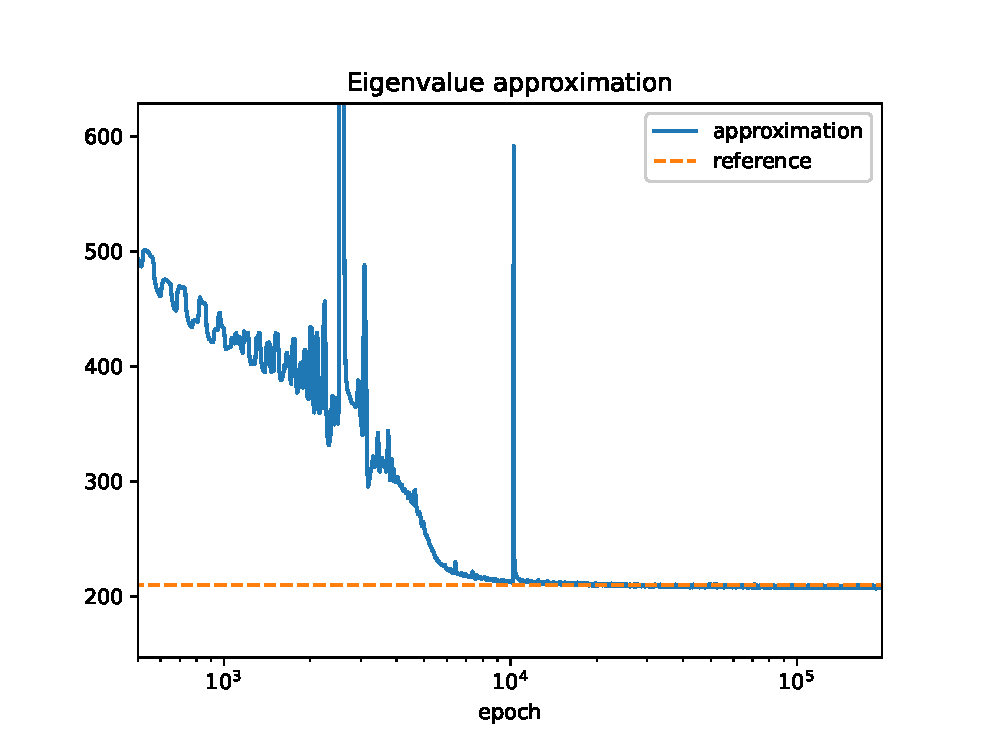
\includegraphics[width=\linewidth]{figures1/20d/eigenvalue_rank2.eps}
%         \caption{单位球上的 $\lambda_{2}$}
%         \label{fig:lambda_rank2}
%     \end{subfigure}
    
%     \vspace{1em} % 增加行间距
    
%     % --- 第三行：Rank 3 ---
%     \begin{subfigure}{0.48\textwidth}
%         \centering
%         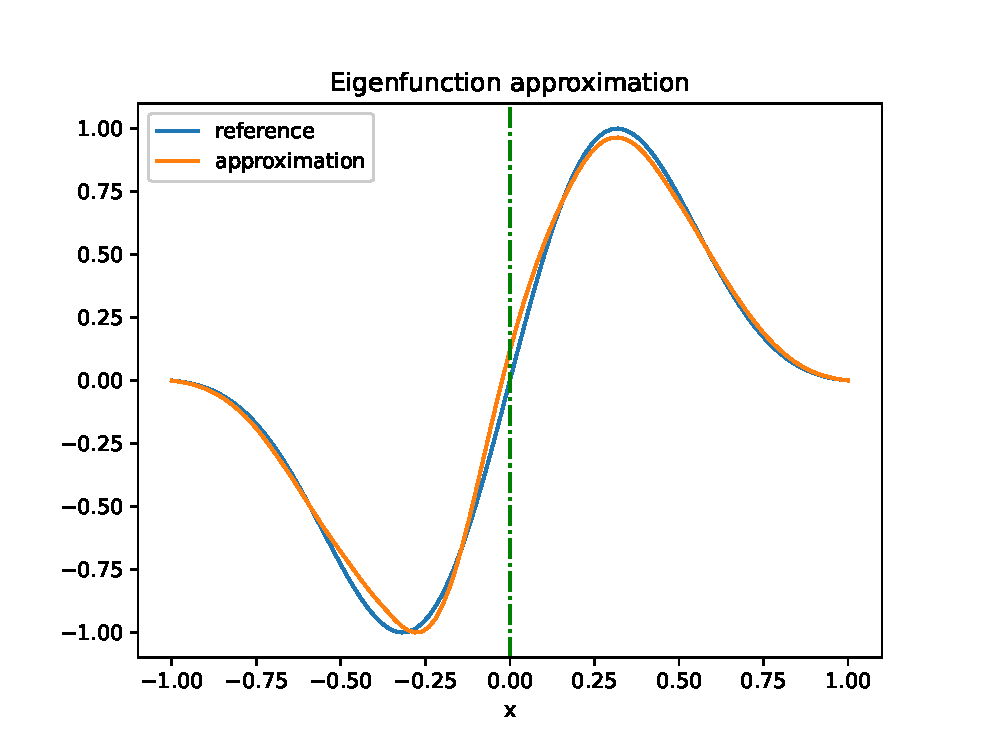
\includegraphics[width=\linewidth]{figures1/20d/unn_rank3.eps}
%         \caption{单位球上的 $\widehat{\xi}_{\phi 3}$}
%         \label{fig:xi_rank3}
%     \end{subfigure}
%     \hfill
%     \begin{subfigure}{0.48\textwidth}
%         \centering
%         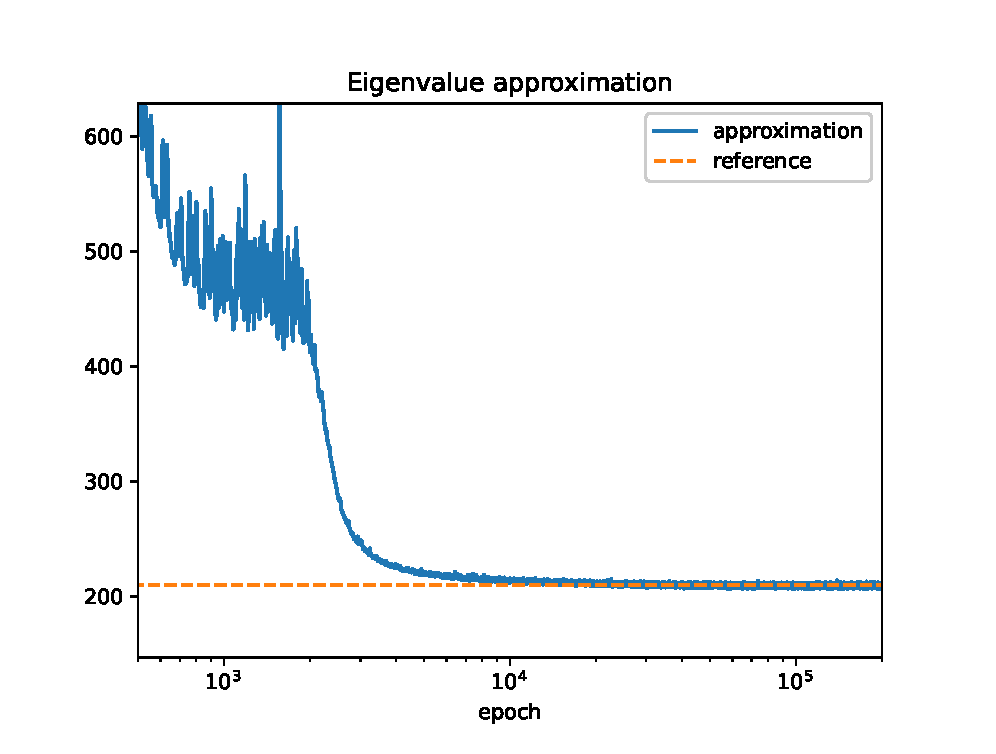
\includegraphics[width=\linewidth]{figures1/20d/eigenvalue_rank3.eps}
%         \caption{单位球上的 $\lambda_{3}$}
%         \label{fig:lambda_rank3}
%     \end{subfigure}
    
%     \caption{左列：20维单位球对角线上的特征函数。右列：特征值随训练轮次（Epoch）的演变情况。}
%     \label{fig:20dball}
% \end{figure}

\section{结论与讨论}\label{sec dis}
本文研究了利用神经网络求解椭圆多重特征值问题。我们基于椭圆特征值问题的惩罚变分形式，提出了一种计算椭圆多重特征值的通用形式。我们利用 Deep Ritz 方法求解了该惩罚变分形式。我们建立了估计特征值与真实特征值之间误差的上界，该上界与网络的深度 $\mathcal{D}$、宽度 $\mathcal{W}$ 以及训练样本量 $n$ 有关。通过探讨特征值问题的正则性并适当选择深度 $\mathcal{D}$ 和宽度 $\mathcal{W}$，我们表明该误差界克服了维数灾难。若干模拟结果证明了所提方法的有效性，并支持了我们的理论结果。

\section{附录}\label{app:proofingen}
\subsection{引理 \ref{lemma:staerr:Rad234} 的证明}
\begin{proof}[引理 \ref{lemma:staerr:Rad234}]\label{pf:lemma:staerr:Rad234}

引理的证明可分为两部分。我们首先证明后四个不等式，这主要依赖于 Rademacher 复杂度的 Lipschitz 收缩不等式：
\begin{lemma}\label{lemma:staerr:liprad}
假设函数 $\psi:\mathbb{R}^{d}\times\mathbb{R}\rightarrow\mathbb{R}$ 满足 $(x,y)\mapsto\psi(x,y)$，且对任意给定的 $x$，其关于 $y$ 是 $\ell$-Lipschitz 连续的。令 $\mathcal{N}$ 为定义在 $\Omega$ 上的函数类，并记 $\psi\circ\mathcal{N}=\{\psi\circ u:x\mapsto\psi(x,u(x)), u\in\mathcal{N}\}$，则有：
$$ \mathfrak{R}(\psi\circ\mathcal{N})\leq\ell \ \mathfrak{R}(\mathcal{N}). $$
\end{lemma}
该引理的严谨推导可参见文献 \cite{ledoux2013probability} 中的推论 3.17。基于此推论，对于引理\ref{lemma:staerr:Rad234}的第二个不等式，由于此情形下的 Lipschitz 常数为 $2\mathcal{B}^{2}$，我们可得：
$$ \sup _{u \in \mathcal{N}^{2}}\left|\mathcal{L}_{k, 2}(u)-\widehat{\mathcal{L}}_{k, 2}(u)\right| \leq |\Omega|\mathfrak{R}\left(\left\{w u^{2}:u\in \mathcal{N}^{2}\right\}\right) \leq 2|\Omega|\mathcal{B}^{2}\mathfrak{R}\left(\mathcal{N}^{2}\right). $$

同理，第三个不等式亦可由此得出，其对应的 Lipschitz 常数为 $2\mathcal{B}$。

至于最后两个不等式，我们使用如下不等式： 
\begin{equation*} 
|a^{2}-b^{2}|\leq 2|a||a-b|+|a-b|^{2}. 
\end{equation*}
利用类似的方法即可推导得出相应结论。

接下来，我们单独处理第一个不等式。由于梯度算子 $\nabla$ 不具备 Lipschitz 连续性，无法直接应用引理 \ref{lemma:staerr:liprad}。为此，我们需要证明 $\nabla u$ 的平方项（即 $|\nabla u|^2$）可由 $\mathrm{ReLU}$-$\mathrm{ReLU}^{2}$ 混合网络实现。具体而言，受 Baur-Strassen 关于多项式及其偏导数计算复杂度的理论启发 \cite{baur1983complexity}，我们提出如下引理：

\begin{lemma}
设 $u$ 为由深度 $\mathcal{D}$、宽度 $\mathcal{W}$ 的 $\mathrm{ReLU}^{2}$ 神经网络所实现的函数，则其梯度的平方项 $|\nabla u|^2$ 可由一个深度不超过 $2\mathcal{D}$、宽度不超过 $(2\mathcal{D}+4)\mathcal{W} + 2d$ 的 $\mathrm{ReLU}$-$\mathrm{ReLU}^{2}$ 混合网络精确表示。
\end{lemma}

\begin{proof}
为表述简便，下文将 $\mathrm{ReLU}$ 与 $\mathrm{ReLU}^{2}$ 激活函数分别记为 $\sigma_1$ 与 $\sigma_2$。容易观察到导数关系 $\sigma_2'(x)=2\sigma_1(x)$。我们将通过构造法来证明本引理。沿用定义 \ref{def:fnn} 中的记号，设 $u^{(k)}$ 为原 $\mathrm{ReLU}^{2}$ 网络第 $k$ 层的激活值，令 $z^{(k)} = W^{(k)}u^{(k-1)} + b^{(k)}$，且 $u^{(k)}=\sigma_2(z^{(k)})$。不失一般性，假设原网络具有单神经元线性输出，即 $u = z_1^{(\mathcal{D})}$。整个构造过程可划分为以下三个阶段：

首先，我们利用 $\mathrm{ReLU}$-$\mathrm{ReLU}^{2}$ 网络重现原网络的前向计算，并同时记录反向推导所需的全部局部导数。记第 $k$ 层的局部导数为 $c^{(k)}$，则有：
$$c^{(k)} = \sigma_2'(z^{(k)}) = 2\sigma_1(z^{(k)})$$
利用 $\sigma_1$ 函数的性质，恒等映射可精确表示为 $x = \sigma_1(x) - \sigma_1(-x)$。因此，在网络传播过程中传递并保留这些局部导数只需使用 $\sigma_1$ 激活函数。为了完整复现原网络的计算并缓存所有局部导数，此阶段需要深度 $\mathcal{D}$。在计算第 $k$ 层时，计算激活值 $u^{(k)}$ 至多消耗 $\mathcal{W}$ 个神经元，而缓存前 $k$ 层的局部导数至多消耗 $2k\mathcal{W}$ 个神经元。由此可知，该阶段的最大宽度受限于 $\mathcal{W} + 2\mathcal{D}\mathcal{W} = (2\mathcal{D}+1)\mathcal{W}$。

第二步，计算伴随变量，这里伴随变量定义为网络输出对各层预激活值的梯度，即 $\delta^{(k)} = \nabla_{z^{(k)}} u$。初始化 $\delta^{(\mathcal{D})} = 1$。根据多元微积分的链式法则，可得如下反向递推关系：
$$\delta_q^{(k)} = c_q^{(k)} \cdot \sum_{p=1}^{n_{k+1}} W_{pq}^{(k+1)} \delta_p^{(k+1)}$$
令 $v_q^{(k)} = \sum_{p=1}^{n_{k+1}} W_{pq}^{(k+1)} \delta_p^{(k+1)}$。注意到 $v_q^{(k)}$ 仅为第 $k+1$ 层伴随变量的线性组合，无需消耗额外的非线性计算深度。利用极化恒等式（$xy=\frac{1}{4}\left[(x+y)^2-(x-y)^2\right]$），两个标量 $c_q^{(k)}$ 与 $v_q^{(k)}$ 的乘法操作可通过一个单隐藏层内包含 $4$ 个 $\sigma_2$ 神经元的子网络精确实现：
$$c_q^{(k)} \cdot v_q^{(k)} = \frac{1}{4}\left[\sigma_2(c_q^{(k)}+v_q^{(k)}) + \sigma_2(-c_q^{(k)}-v_q^{(k)}) - \sigma_2(c_q^{(k)}-v_q^{(k)}) - \sigma_2(-c_q^{(k)}+v_q^{(k)})\right]$$
我们将原网络的计算图进行反向展开，针对 $k$ 从 $\mathcal{D}-1$ 递减至 $1$，逐层构造上述乘法子网络以计算 $\delta^{(k)}$。由于 $c_q^{(k)}$ 和 $v_q^{(k)}$ 均可由已有的网络节点通过线性组合获得，每次计算 $\delta^{(k)}$ 仅需通过 $1$ 层 $\sigma_2$ 激活函数。该反向递推共需进行 $\mathcal{D}-1$ 次，因此本阶段消耗的深度为 $\mathcal{D}-1$。在每层中，至多需要并行计算 $\mathcal{W}$ 个乘法，消耗 $4\mathcal{W}$ 个神经元。同时，网络需要继续向下层传递剩余未使用的缓存变量 $c^{(1)}, \dots, c^{(k-1)}$，这部分占用至多 $2(\mathcal{D}-1)\mathcal{W}$ 个神经元。因此，此阶段的最大宽度界限为 $4\mathcal{W} + 2\mathcal{D}\mathcal{W}$

第三步，计算梯度并平方求和：当递推至第一层并获得 $\delta^{(1)}$ 后，即可一次性求出针对所有 $d$ 个输入变量的偏导数：
$$\partial_i u = \sum_{p=1}^{n_1} W_{pi}^{(1)} \delta_p^{(1)}, \quad i=1, 2, \dots, d$$
最后，计算梯度向量模长的平方：
$$|\nabla u|^2 = \sum_{i=1}^d (D_i u)^2 = \sum_{i=1}^d \left[ \sigma_2(D_i u) + \sigma_2(-D_i u) \right]$$
由于求偏导数 $D_iu$ 属于线性映射，最终的平方与求和操作只需增加 $1$ 层 $\sigma_2$ 非线性层。在此最终层内，需并行计算 $d$ 个维度分量的平方展开项，共消耗 $2d$ 个神经元。

将上述三个阶段级联，所构造的目标混合网络的总复杂度受限于：
\begin{itemize}
    \item 总深度： $\mathcal{D}\left(|\nabla u|^2\right) = \mathcal{D} + (\mathcal{D}-1) + 1 = 2\mathcal{D}$
    \item 总宽度： 取各计算阶段宽度的最大值：
    $$\mathcal{W}\left(|\nabla u|^2\right) \leq \max\left\{ (2\mathcal{D}+1)\mathcal{W}, \ 2d \right\} \leq (2\mathcal{D}+4)\mathcal{W} + 2d$$
\end{itemize}


\end{proof}

\end{proof}

\subsection{引理 \ref{lemma:staerr:Rad_cover} 的证明}
\begin{proof}[引理 \ref{lemma:staerr:Rad_cover}]\label{pf:lemma:staerr:Rad_cover}
首先，我们引入 Massart 有限类引理（Massart's finite class lemma），其详细证明可参阅文献 \cite{boucheron2013concentration}。

\begin{lemma}[Massart 有限类引理 \cite{boucheron2013concentration}]\label{Mfinite}
对于任意给定的有限集 $V\subset\mathbb{R}^{n}$，记其最大向量 $\ell_2$ 范数为 $D=\sup_{v\in V}\|v\|_{2}$。则有：
$$ \mathbb{E}_{\Sigma_{n}}\left[ \sup_{v\in V}\frac{1}{n}\left| \sum_{i=1}^{n}\sigma_{i}v_{i} \right| \right] \leq \frac{D}{n}\sqrt{2\log(2|V|)}, $$
其中 $\sigma_{i}$ 和 $\mathbb{E}_{\Sigma_{n}}$ 分别为定义 \ref{def:staerr:radcom} 中所述的 Rademacher 随机变量及其期望。
\end{lemma}
接下来，我们采用标准的链式推导（Chaining Method）。令 $\varepsilon_{k}=2^{-k+1} B$。记 $\mathcal{F}_{k}$ 为 $\mathcal{F}$ 在无穷范数下的一个 $\varepsilon_{k}$-覆盖集，其基数满足 $\left|\mathcal{F}_{k}\right|=\mathcal{C}\left(\varepsilon_{k}, \mathcal{F},\|\cdot\|_{\infty}\right)$。这意味着，对于任意函数 $u \in \mathcal{F}$，必定存在 $u_{k} \in \mathcal{F}_{k}$ 使得 $\left\|u-u_{k}\right\|_{\infty} \leq \varepsilon_{k}$。令 $K$ 为一个待定的正整数。通过项的分解与三角不等式，我们有：

$$ \begin{aligned} 
    &\quad\; \mathbb{E}_{\left\{\sigma_{i}, Z_{i}\right\}_{i=1}^{n}}\left[\sup\limits_{u \in \mathcal{F}} \frac{1}{n}\left|\sum\limits_{i=1}^{n} \sigma_{i} u\left(Z_{i}\right)\right|\right] \\ &= \mathbb{E}_{\left\{\sigma_{i}, Z_{i}\right\}_{i=1}^{n}}\left[\sup\limits _{u \in \mathcal{F}} \frac{1}{n}\left|\sum\limits_{i=1}^{n} \sigma_{i}\left(u\left(Z_{i}\right)-u_{K}\left(Z_{i}\right)\right) + \sum\limits_{j=1}^{K-1} \sum\limits_{i=1}^{n} \sigma_{i}\left(u_{j+1}\left(Z_{i}\right)-u_{j}\left(Z_{i}\right)\right) + \sum\limits_{i=1}^{n} \sigma_{i} u_{1}\left(Z_{i}\right)\right|\right] \\ &\leq \mathbb{E}_{\left\{\sigma_{i}, Z_{i}\right\}_{i=1}^{n}}\left[\sup\limits _{u \in \mathcal{F}} \frac{1}{n}\left|\sum\limits_{i=1}^{n} \sigma_{i}\left(u\left(Z_{i}\right)-u_{K}\left(Z_{i}\right)\right)\right|\right] \\ &\quad + \sum\limits_{j=1}^{K-1} \mathbb{E}_{\left\{\sigma_{i}, Z_{i}\right\}_{i=1}^{n}}\left[\sup\limits _{u \in \mathcal{F}} \frac{1}{n}\left|\sum\limits_{i=1}^{n} \sigma_{i}\left(u_{j+1}\left(Z_{i}\right)-u_{j}\left(Z_{i}\right)\right)\right|\right] \\ &\quad + \mathbb{E}_{\left\{\sigma_{i}, Z_{i}\right\}_{i=1}^{n}}\left[\sup\limits _{u \in \mathcal{F}} \frac{1}{n}\left|\sum\limits_{i=1}^{n} \sigma_{i} u_{1}\left(Z_{i}\right)\right|\right]. 
\end{aligned} $$
由于零函数 $0 \in \mathcal{F}$，我们可以无妨设定 $\mathcal{F}_{1}=\{0\}$，从而消除上述不等式中的第三项。对于第一项，应用 Rademacher 变量的性质与 Hölder 不等式：
\begin{equation*}
\begin{aligned}
{}&\mathbb{E}_{\left\{\sigma_{i}, Z_{i}\right\}_{t=1}^{n}}\left[\sup\limits _{u \in \mathcal{F}} \frac{1}{n}\left|\sum\limits_{i=1}^{n} \sigma_{i}\left(u\left(Z_{i}\right)-u_{K}\left(Z_{i}\right)\right)\right|\right]\\
\leq&\mathbb{E}_{\left\{\sigma_{i}, Z_{i}\right\}_{i=1}^{n}}\left[\sup\limits _{u \in \mathcal{F}} \frac{1}{n} \sum\limits_{i=1}^{n}\left|\sigma_{i}\right|\left\|u-u_{K}\right\|_{\infty}\right] \leq \varepsilon_{K}
\end{aligned}
\end{equation*}
对于第二项中的求和单元，定义向量 $v_{i}^{j}=u_{j+1}\left(Z_{i}\right)-u_{j}\left(Z_{i}\right)$，并应用引理 \ref{Mfinite}，得到：
\begin{equation*}
\begin{aligned}
&\sum_{j=1}^{K-1} \mathbb{E}_{\{\sigma\}_{i=1}^{n}}\left[\sup _{u \in \mathcal{F}} \frac{1}{n}\left|\sum_{i=1}^{n} \sigma_{i}\left(u_{j+1}\left(Z_{i}\right)-u_{j}\left(Z_{i}\right)\right)\right|\right]\\
=&\sum_{j=1}^{K-1} \mathbb{E}_{\left\{\sigma_{t}\right\}_{t=1}^{n}}\left[\sup _{v \in V_{j}} \frac{1}{n} \left| \sum_{i=1}^{n} \sigma_{i} v_{i}^{j}\right|\right] \leq \sum_{j=1}^{K-1} \frac{D_{j}}{n} \sqrt{2 \log \left(2\left|V_{j}\right|\right)}.
\end{aligned}
\end{equation*}
根据集合 $V_{j}$ 的构造，其势满足界限 $\left|V_{j}\right| \leq\left|\mathcal{F}_{j}\right|\left|\mathcal{F}_{j+1}\right| \leq\left|\mathcal{F}_{j+1}\right|^{2}$。同时，向量的范数上界 $D_j$ 可被限制为：
$$ \begin{aligned}
     D_j &= \sup_{v \in V_j} \left(\sum_{i=1}^{n}\left|u_{j+1}\left(Z_{i}\right)-u_{j}\left(Z_{i}\right)\right|^{2}\right)^{1 / 2} \leq \sqrt{n}\left\|u_{j+1}-u_{j}\right\|_{\infty} \\ &\leq \sqrt{n}\left\|u_{j+1}-u\right\|_{\infty}+\sqrt{n}\left\|u_{j}-u\right\|_{\infty} = \sqrt{n} \varepsilon_{j+1}+\sqrt{n} \varepsilon_{j} = 3 \sqrt{n} \varepsilon_{j+1}. 
\end{aligned} $$
将其代入前式，有：
\begin{equation*}
\begin{aligned}
&\sum_{j=1}^{K-1} \mathbb{E}_{\left\{\sigma_{i}, Z_{t}\right\}_{t=1}^{n}}\left[\sup _{u \in \mathcal{F}} \frac{1}{n}\left|\sum_{i=1}^{n} \sigma_{i}\left(u_{j+1}\left(Z_{i}\right)-u_{j}\left(Z_{i}\right)\right)\right|\right] \\
&\leq \sum_{j=1}^{K-1} \frac{D_{j}}{n} \sqrt{2 \log \left(2\left|V_{j}\right|\right)} \leq \sum_{j=1}^{K-1} \frac{3 \varepsilon_{j+1}}{\sqrt{n}} \sqrt{2 \log \left(2\left|\mathcal{F}_{j+1}\right|^{2}\right)}
\end{aligned}
\end{equation*}
结合上述所有界的估计，我们将离散求和转化为 Dudley 积分形式：
\begin{equation*}
\begin{aligned}
&\mathbb{E}_{\left\{\sigma_{i}, Z_{i}\right\}_{i=1}^{n}}\left[\sup _{u \in \mathcal{F}} \frac{1}{n}\left|\sum_{i=1}^{n} \sigma_{i} u\left(Z_{i}\right)\right|\right] \leq \varepsilon_{K}+\sum_{j=1}^{K-1} \frac{6 \varepsilon_{j+2}}{\sqrt{n}} \sqrt{2 \log \left(2\left|\mathcal{F}_{j+1}\right|^{2}\right)} \\
&=\varepsilon_{K}+\frac{6}{\sqrt{n}} \sum_{j=1}^{K-1}\left(\varepsilon_{j+1}-\varepsilon_{j+2}\right) \sqrt{2 \log \left(2 \mathcal{C}\left(\varepsilon_{j+1}, \mathcal{F},\|\cdot\|_{\infty}\right)^{2}\right)}\\
&\leq \varepsilon_{K}+\frac{6}{\sqrt{n}} \int_{\varepsilon_{K+1}}^{B / 2} \sqrt{2 \log \left(2 \mathcal{C}\left(\varepsilon, \mathcal{F},\|\cdot\|_{\infty}\right)^{2}\right)} d \varepsilon.
\end{aligned}
\end{equation*}
最后，对于任意给定的精度 $0<\delta<\frac{B}{2}$，我们总可以通过选取充分大的 $K$ 使得 $\varepsilon_{K+2}<\delta \leq \varepsilon_{K+1}$，从而完成引理的证明。
\end{proof}

\subsection{引理 \ref{lemma:staerr:pdim} 的证明}
\begin{proof}[引理 \ref{lemma:staerr:pdim}]\label{pf:lemma:staerr:pdim}
本引理的证明思路如下：首先，我们回顾打散与 VC 维的严格定义。

为了估计多项式的 Pdim，我们引入以下引理（其详细证明见文献 \cite{anthony2009neural} 的定理 8.3）：

\begin{lemma}\label{lemma:covering_number}
设 $p_1,\cdots,p_m$ 为 $m$ 个具有 $n$ 个变量且最高次数不超过 $d$ 的多项式。若 $n \leq m$，则这些多项式符号组合的集合基数满足：
\begin{equation*}
|{(\operatorname{sign}(p_1(x)),\cdots,\operatorname{sign}(p_m(x))):x\in\mathbb{R}^n}| \leq 2\left(\frac{2emd}{n}\right)^n
\end{equation*}

\end{lemma}
接下来的论证借鉴了文献 \cite{bartlett2019nearly} 中定理 6 的分析框架。需要指出的是，由于 $\mathrm{VCdim}(\operatorname{sign}(\mathcal{N})) \leq \mathrm{Pdim}(\mathcal{N})$，此处推导出的结论比原定理略强。

我们构造一个新的示性函数族： 
\begin{equation*}
\mathcal{\widetilde{N}}={\widetilde{u}(x,y)=\operatorname{sign}(u(x)-y): u\in\mathcal{N}}
\end{equation*}

根据定义，显然有 $\mathrm{Pdim}(\mathcal{N}) \leq \mathrm{VCdim}(\widetilde{\mathcal{N}})$。因此，问题转化为界定 $\widetilde{\mathcal{N}}$ 的 VC 维。设 $\mathcal{M}$ 为实现 $\mathcal{N}$ 中函数的神经网络的参数（权重与偏置）总数。对于任意给定的点集 $\{x_i\}_{i=1}^{m}\subset X$ 和 $\{y_i\}_{i=1}^{m}\subset\mathbb{R}$，我们考察由网络参数 $a \in \mathbb{R}^{\mathcal{M}}$ 诱导的二分法（dichotomies）数量：
\begin{equation*}
K_{{x_i},{y_i}}(m):=|{(\operatorname{sign}(u(x_{1}, a)-y_1), \ldots, \operatorname{sign}(u(x_{m}, a)-y_m)): a \in \mathbb{R}^{\mathcal{M}}}|
\end{equation*}
由定义可知，$K_{\{x_i\},\{y_i\}}(m)$ 在所有可能的 $\{x_i\}_{i=1}^{m}$ 与 $\{y_i\}_{i=1}^{m}$ 上的上确界，即为函数族 $\widetilde{\mathcal{N}}$ 的增长函数（Growth function） $\mathcal{G}_{\widetilde{\mathcal{N}}}(m)$。

为了能够应用引理 \ref{lemma:covering_number}，我们需要将参数空间 $\mathbb{R}^{\mathcal{M}}$ 划分为若干子区域，使得在每一个子区域内，网络输出 $u(x_i,a)-y_i$ 关于参数 $a$ 均表现为无断点（breakpoints）的多项式。沿用文献 \cite{bartlett2019nearly} 中的划分策略，我们将参数空间划分为 $\{P_1,P_2,\cdots,P_N\}$，其中区域总数 $N$ 满足：
\begin{equation} \label{pdimb1}
N\leq\prod_{i=1}^{\mathcal{D}-1}2\left(\frac{2emk_i(1+(i-1)2^{i-1})}{\mathcal{M}i}\right)^{\mathcal{M}i}
\end{equation}
上式中，$k_i$ 表示神经网络第 $i$ 层的神经元数量，而 $\mathcal{M}_i$ 表示截至第 $i$ 层（包含第 $i$ 层）所有神经元输入的参数总数。基于此划分，二分法总数可由各子区域内的二分法数量之和控制：
\begin{equation} \label{pdimb2}
K_{{x_i},{y_i}}(m)\leq\sum_{i=1}^{N}|{(\operatorname{sign}(u(x_{1}, a)-y_1), \cdots, \operatorname{sign}(u(x_{m}, a)-y_m)): a\in P_i}|
\end{equation}

注意到在每个子区域 $P_i$ 内，$u(x_i,a)-y_i$ 是关于 $a$ 的多项式。如文献 \cite{bartlett2019nearly} 所证，该多项式的次数与其自身次数一致，且上界为 $1 + (\mathcal{D}-1)2^{\mathcal{D}-1}$。因此，直接应用引理 \ref{lemma:covering_number} 可得每个子区域的界：
\begin{align}
& |{(\operatorname{sign}(u(x_{1}, a)-y_1), \cdots, \operatorname{sign}(u(x_{m}, a)-y_m)): a\in P_i}|\nonumber \\
& \leq2\left(\frac{2em(1+(\mathcal{D}-1)2^{\mathcal{D}-1})}{\mathcal{M}{\mathcal{D}}}\right)^{\mathcal{M}{\mathcal{D}}}\label{pdimb3}.
\end{align}
将式 (\ref{pdimb1}) 和 (\ref{pdimb3}) 代入式 (\ref{pdimb2}) 中，可推导出：
\begin{equation*}
K_{{x_i},{y_i}}(m)\leq\prod_{i=1}^{\mathcal{D}}2\left(\frac{2emk_i(1+(i-1)2^{i-1})}{\mathcal{M}_i}\right)^{\mathcal{M}i}.
\end{equation*}
由于该上界对所有样本点集均一致成立，故增长函数满足：
\begin{equation*}
\mathcal{G}_{\widetilde{\mathcal{N}}}(m)\leq\prod_{i=1}^{\mathcal{D}}2\left(\frac{2emk_i(1+(i-1)2^{i-1})}{\mathcal{M}_i}\right)^{\mathcal{M}_i},
\end{equation*}
最终，通过类似于文献 \cite{bartlett2019nearly} 中定理 6 的代数化简（令 $\mathcal{G}_{\widetilde{\mathcal{N}}}(m) < 2^m$ 并求解 $m$ 的界），我们可得：
\begin{equation*}
\mathrm{Pdim}(\mathcal{N})\lesssim C\left(\mathcal{D}^2\mathcal{W}^2 \log \mathcal{U}+\mathcal{D}^3\mathcal{W}^2\right)
\lesssim C\left(\mathcal{D}^2\mathcal{W}^2\left( \mathcal{D}+\log \mathcal{W}\right)\right)
\end{equation*}
其中常数 $C$ 与网络架构无关，$\mathcal{U}$ 为实现函数族 $\mathcal{N}$ 的神经网络中包含的神经元总数。至此，引理得证。
\end{proof}



%%%%==========================================================%%%

\chapter{深度里兹法求解拟线性偏微分方程}
% \section{预备知识与记号}\label{sec:pre}
% 在本文中，我们考虑如下半线性椭圆方程：
% \begin{equation}\label{eq:maineq}
% \left\{\begin{aligned}
% -\Delta u+f(u) &=g & & \text { in } \Omega \\
%  u + \frac{1}{\varepsilon}\frac{\partial u}{\partial n} &=h & & \text { on } \partial \Omega
% \end{aligned}\right.
% \end{equation}
% 其中 $\varepsilon\in (0,+\infty]$。$\varepsilon$ 的区间包含了 Dirichlet 边界条件 ($\varepsilon=+\infty$) 和 Robin 边界条件 ($\varepsilon\in (0,+\infty)$) 的情形。
% 我们对方程施加如下限制：

% \begin{remark}\label{ass:f}
% \begin{itemize}
% \item $\Omega\subset \mathbb{R}^{d}$ 是有界且光滑的。
% \item 对于某个常数 $C$，满足 $|f(x)|\leq C\left(|x|+1\right)^{\frac{d}{d-2}}$。$f$ 是 Lipschitz 连续且单调递增的。
% \item 对于某个 $p\geq 2$，有 $g\in L^{p}$。
% \item 在 $\Omega^{'}\supset \bar{\Omega}$ 上存在一个调和函数 $w$，使得
% $
% w+\frac{1}{\varepsilon}\frac{\partial w}{\partial n}=h
% $
% 在 $\partial \Omega$ 上成立。
% \end{itemize}

% 我们记 $F$ 为 $f$ 的原函数，因此 $F$ 是一个凸函数。
% \end{remark}

% 根据 Schauder 理论可得：

% \begin{theorem}
% 在假设 \ref{ass:f} 下，可知存在且唯一存在一个 $u^{\varepsilon} \in W^{2,2}(\Omega)$ 作为方程~\eqref{eq:maineq} 的解，且 $\|u^{\varepsilon}\|_{W^{2,2}}$ 可被 $g$ 和 $h$ 控制。
% \end{theorem}
% \begin{proof}
% 参见 \cite{2013Roubiek} 中的命题 2.104。
% \end{proof}

% 接下来，介绍我们所使用的神经网络及其记号。深度神经网络 $u_{\phi}:\mathbb{R}^{d}\rightarrow\mathbb{R}$ 定义为
% \begin{equation*}
% \begin{aligned}
% &u_{0}(\boldsymbol{x})=\boldsymbol{x} \\
% &u_{\ell}(\boldsymbol{x})=\sigma_{\ell}\left(A_{\ell} u_{\ell-1}+b_{\ell}\right), \quad \ell=1,2, \ldots, L-1 \\
% &u=u_{L}(\boldsymbol{x})=A_{L} u_{L-1}+b_{L}
% \end{aligned}
% \end{equation*}
% 其中 $A_{\ell}\in\mathbb{R}^{N_{\ell}\times N_{\ell-1}}$, $b_{\ell}\in\mathbb{R}^{N_{\ell}}$，且 $\sigma_{\ell}$ 表示第 $\ell$ 层的激活函数。神经网络 $u_{\phi}$ 的深度 $\mathcal{D}$ 和宽度 $\mathcal{W}$ 定义为
% \begin{equation*}
% \mathcal{D}=L, \ \mathcal{W}=\max\{N_{\ell}:\ell=1,2,\ldots,L\}.
% \end{equation*}
% $\sum_{\ell=1}^{L}N_{\ell}$ 称为 $u_{\phi}$ 的单元数，而 $\phi=\{A_{\ell},b_{\ell}\}_{\ell=1}^{N}$ 称为网络的自由参数。
% \begin{definition}
% 类 $\mathcal{N}^{\alpha}(\mathcal{D},\mathcal{W},\mathcal{B})$ 是满足以下条件的神经网络 $u_{\phi}$ 的集合：
% \begin{itemize}
% \item[(i)] 深度和宽度分别为 $\mathcal{D}$ 和 $\mathcal{W}$；
% \item[(ii)] $u_{\phi}(\boldsymbol{x})$ 的函数值及其导数 $\nabla u_{\phi}(\boldsymbol{x})$ 被 $\mathcal{B}$ 有界控制；
% \item[(iii)] 激活函数由 $\mathrm{ReLU}^{\alpha}$ 给出，其中 $\alpha$ 是一个（多重）指标。
% \end{itemize}
% \end{definition}
% 例如，$\mathcal{N}^{2}(\mathcal{D},\mathcal{W},\mathcal{B})$ 是激活函数为 $\mathrm{ReLU}^2$ 的网络类，而 $\mathcal{N}^{1,2}(\mathcal{D},\mathcal{W},\mathcal{B})$ 是激活函数为 $\mathrm{ReLU}^1$ 或 $\mathrm{ReLU}^2$ 的网络类。若无歧义，我们可以简单地使用 $\mathcal{N}^\alpha$。

% \section{模型构建}\label{sec:mod}

% \begin{theorem}\label{thm:model}
% 对于 $v\in H^{1}(\Omega)$，令
% \begin{equation}\label{eq:conloss}
% \mathcal{L}^{\varepsilon}(v) = \int_{\Omega} \|\nabla v\|_{2}^{2} + 2F(v) - 2vg\,dx + \varepsilon \int_{\partial \Omega}v^{2} - 2vh\,ds.
% \end{equation}
% 则
% \begin{itemize}
% \item 对于 $\varepsilon\in (0,+\infty)$，$\mathcal{L}^{\varepsilon}$ 存在唯一的极小值点，记为 $u^{\varepsilon}$。它是方程 Eq.~\eqref{eq:maineq} 的解。
% \item 当 $\varepsilon \rightarrow +\infty$ 时，设 $u^{\infty}$ 为具有 Dirichlet 边界条件的方程 Eq.~\eqref{eq:maineq} 的解。则我们有：

% \textcolor{black}{\begin{equation*}
% \|u^{\varepsilon}-u^{\infty}\|_{H^{1}}\leq C(\Omega,f,g,h)\frac{1}{\varepsilon}.
% \end{equation*}}

% \end{itemize}
% \end{theorem}
% \begin{proof}
% 如果 $\varepsilon<+\infty$，Eq.~\eqref{eq:conloss} 的欧拉-拉格朗日方程可写为：
% \begin{equation*}
% \begin{array}{rcl}
% \delta \mathcal{L}^{\varepsilon}(v)&=&\displaystyle 2\int_{\Omega}\nabla v^{T}\nabla \delta v + f(v) \delta v - g\delta v\,dx + 2\varepsilon\int_{\partial \Omega}(v-h)\delta v\,ds\\
% {}&=&\displaystyle 2\int_{\Omega} \left(-\Delta v+f(v)-g\right)\delta v\,dx + 2\varepsilon\int_{\partial \Omega} \left(v+\frac{1}{\varepsilon}\frac{\partial v}{\partial n}-h\right) \delta v\,ds.\\
% \end{array}
% \end{equation*}

% Eq.~\eqref{eq:conloss} 的所有临界点必须是 Eq.~\eqref{eq:maineq} 的解，反之亦然。因此，存在唯一的临界点。此外，Eq.~\eqref{eq:conloss} 的凸性保证了该临界点即为极小值点。

% 考虑到 Dirichlet 边界条件，我们将 $w^{\varepsilon}$ 设置为满足以下方程的解：
% \begin{equation*}
% \left\{\begin{aligned}
% -\Delta w^{\varepsilon} +f(u^{\infty})&=g \quad \text { 在 } \Omega \text{ 中} \\
%  w^{\varepsilon}+\frac{1}{\varepsilon}\frac{\partial w^{\varepsilon}}{\partial n} &=h \quad \text { 在 } \partial \Omega \text{ 上},
% \end{aligned}\right.
% \end{equation*}
% 已知（参见 \cite{Maury2009Numerical}（命题 2.3 的证明））：
% $\|w^{\varepsilon}-u^{\infty}\|_{H^{1}}\leq C(\Omega,f(u^{\infty}),g,h)\frac{1}{\varepsilon}$。
% 经典的线性椭圆理论为我们提供了：
% \begin{equation*}
% \int_{\Omega}\|\nabla (w^{\varepsilon}-u^{\varepsilon})\|_{2}^{2}\,dx + \varepsilon \int_{\partial \Omega}(w^{\varepsilon}-u^{\varepsilon})^{2}\,ds \leq \|f(u^{\infty})-f(u^{\varepsilon})\|^{2}_{H^{-1}}\leq C(\Omega,f,u^{\infty}),
% \end{equation*}
% 给定 $f(u^{\varepsilon}),f(u^{\infty})\in L^{2}$。
% 则 $\{u^{\varepsilon}\}$ 是 $H^{1}$ 中的有界序列。但是
% \begin{equation}\label{eq:seminormcontrol}
% \begin{array}{rcl}
% \displaystyle\int_{\Omega}\|\nabla(u^{\infty}-u^{\varepsilon})\|_{2}^{2}\,dx&=&\displaystyle\int_{\Omega}\nabla (u^{\infty}-u^{\varepsilon})^{T}\nabla u^{\infty}\,dx-\int_{\Omega}\nabla (u^{\infty}-u^{\varepsilon})^{T}\nabla u^{\varepsilon}\,dx\\
% {}&{}&{}\\
% {}&=&\displaystyle\int_{\Omega}-\left(u^{\infty}-u^{\varepsilon}\right)\Delta u^{\infty}\,dx-\int-\left( u^{\infty}-u^{\varepsilon}\right)\Delta u^{\varepsilon}\,dx +\\
% {}&{}&\displaystyle\int_{\partial \Omega}\frac{\partial u^{\infty}}{\partial n}(u^{\infty}-u^{\varepsilon})\,ds-\int_{\partial \Omega}\frac{\partial u^{\varepsilon}}{\partial n}(u^{\infty}-u^{\varepsilon})\,ds\\
% {}&{}&{}\\
% {}&=&\displaystyle-\int_{\Omega} \left[f(u^{\infty})-f(u^{\varepsilon})\right]\left(u^{\infty}-u^{\varepsilon}\right)\,dx \\
% {}&{}&\displaystyle+\frac{1}{\varepsilon} \int_{\partial \Omega}\frac{\partial u^{\infty}}{\partial n}\frac{\partial u^{\varepsilon}}{\partial n}\,ds-\frac{1}{\varepsilon} \int_{\partial \Omega}\left(\frac{\partial u^{\varepsilon}}{\partial n}\right)^{2}\,ds\\
% {}&{}&{}\\
% {}&\leq&\displaystyle\frac{1}{2\varepsilon}\left[\int_{\partial \Omega}\left(\frac{\partial u^{\infty}}{\partial n}\right)^{2}-\left(\frac{\partial u^{\varepsilon}}{\partial n}\right)^{2}\,ds\right]\leq C(\Omega,f,g,h)\frac{1}{\varepsilon},
% \end{array}
% \end{equation}
% 注意到 $f$ 是非递减的。
% 接下来，我们将 $u^{\infty}$ 代入 $\mathcal{L}^{\varepsilon}$，得到：
% \begin{equation*}
% \mathcal{L}^{\varepsilon}(u^{\varepsilon})\leq \mathcal{L}^{\varepsilon}(u^{\infty}) \leq C(\Omega,f,g,h) - \varepsilon\int_{\partial \Omega}h^{2}。
% \end{equation*}
% 因此
% \begin{equation*}
% \varepsilon\int_{\partial \Omega}(u^{\varepsilon}-h)^{2}\leq C(\Omega,f,g,h)。
% \end{equation*}
% 结合等式~\eqref{eq:seminormcontrol}，我们可以推导出所需的结论。

% \end{proof}

% 转到 DRM 的第二步，我们将试探函数替换为神经网络：
% \begin{equation*}
% u^{\varepsilon}_{\phi}\in \underset{v \in \mathcal{N}^{2}}{\operatorname{argmin}}\,\mathcal{L}^{\varepsilon}(v),
% \end{equation*}
% 损失函数的离散形式表示如下\cite{chen2021quasi}：
% \begin{equation}\label{eq:disloss}
% \begin{aligned}
% \widehat{\mathcal{L}}_{K}^{\varepsilon}(v) = & \frac{|\Omega|}{N}\sum\limits_{i=1}^{N} \left[ \|\nabla v(X_{i})\|_{2}^{2}+2F\left(v(X_{i})\right)-2g_{K}(X_{i})v(X_{i})\right]\\
% &+\varepsilon\frac{|\partial\Omega|}{M}\sum\limits_{j=1}^{M}\left[v^{2}(Y_{j})-2v(Y_{j})h(Y_{j})\right],
% \end{aligned}
% \end{equation}
% 其中 $\{X_{k}\}_{k=1}^{N}\sim U(\Omega)$ 独立同分布，$\{Y_{j}\}_{j=1}^{M}\sim U(\partial\Omega)$ 独立同分布，且 $g_{K} = \min\{g,K\}$，$K$ 为某个常数。引入截断界 $K$ 是为了避免离散 $\mathcal{L}^{\varepsilon}$ 的不连续性。设 $\widehat{u}^{\varepsilon}_{\phi}$ 为 $\mathcal{N}^{2}$ 上该损失的极小值点：
% \begin{equation}\label{eq:u_hat}
% \widehat{u}^{\varepsilon}_{\phi}\in \underset{v \in \mathcal{N}^{2}}{\operatorname{argmin}}\,\widehat{\mathcal{L}}_{K}^{\varepsilon}(v),
% \end{equation}
% 在随后的讨论中，我们用 $n$ 表示样本数 $N$ 或 $M$。

% \begin{lemma}\label{lemma:energyerr}
% 令 $\widehat{u}^{\varepsilon}_{\phi}$ 为上文定义的函数，我们有：
% \begin{equation*}
% \begin{array}{rcl}
% {}&{}&\mathcal{L}^{\varepsilon}\left(\widehat{u}_{\phi}^{\varepsilon}\right)-\mathcal{L}^{\varepsilon}(u^{\varepsilon})\\
% {}&{}&{}\\
% {}&\leq&\displaystyle\underbrace{ \inf _{u_{\phi} \in \mathcal{N}^{2}}\left[ \mathcal{L}^{\varepsilon}(u_{\phi})- \mathcal{L}^{\varepsilon}(u^{\varepsilon})\right]}_{\mathcal{E}_{\text{app}}}+\underbrace{2 \sup _{u_{\phi} \in \mathcal{N}^{2}}\left|\mathcal{L}^{\varepsilon}_{K}(u_{\phi})-\widehat{\mathcal{L}}^{\varepsilon}_{K}(u_{\phi})\right|}_{\mathcal{E}_{\text{sta}}}+\underbrace{C(g)\mathcal{B}K^{1-p}}_{\mathcal{E}_{\text{tru}}},\\
% \end{array}
% \end{equation*}
% 它们分别被称为逼近误差、统计误差和截断误差。
% \end{lemma}
% \begin{proof}
% 首先，我们介绍一个关于截断误差的简单引理：

% \begin{lemma}\label{lemma:truerr}
% 设 $1\leq q<p<\infty$。如果 $u\in L^{p}$ 且 $u_{N}=u1_{|u|<N}$，则我们有：
% \begin{equation*}
% \|u-u_{N}\|_{L^{q}}\leq C(u)\frac{1}{N^{p/q-1}}.
% \end{equation*}
% \end{lemma}
% \begin{proof}
% 设 $v = |u-u_{N}|$，$f_{v}(t)=m(\{x:v(x)<t\})$，其中 $m$ 是 \textcolor{black}{Lebesgue 测度}。
% \begin{equation*}
% \begin{array}{rcl}
% \|v\|_{L^{q}}^{q}&=&\displaystyle q\int_{0}^{\infty}t^{q-1}f_{v}(t)\,dt\\
% {}&{}&{}\\
% {}&=&\displaystyle q\int_{N}^{\infty}t^{p-1}f_{v}(t)t^{q-p}\,dt\\
% {}&{}&{}\\
% {}&=&\displaystyle qN^{q-p}\int_{N}^{\infty}t^{p-1}f_{v}(t)\,dt\\
% {}&{}&{}\\
% {}&=&\displaystyle qN^{q-p}\|v\|_{L^{p}}^{p}
% \end{array}
% \end{equation*}
% 这便导出了结论。
% \end{proof}
% 令
% \begin{equation*}
% \mathcal{L}_{K}^{\varepsilon}(v)=\int_{\Omega}\|\nabla v\|_{2}^{2}+2 F(v)-2 v g_{K}\,d x+\varepsilon \int_{\partial \Omega} v^{2}-2 v h d s.
% \end{equation*}
% 借助引理 \ref{lemma:truerr}，我们有：
% \begin{equation*}
% |\mathcal{L}_{K}^{\varepsilon}(u_{\phi})-\mathcal{L}^{\varepsilon}(u_{\phi})|\leq\int_{\Omega}|u_{\phi}(g-g_{K})|\,dx\leq C(g)\mathcal{B}K^{1-p},
% \end{equation*}
% 对于任意 $u_{\phi}\in \mathcal{N}^{2}(\mathcal{D},\mathcal{W},\mathcal{B})$。
% 因此，对于任意 $u\in \mathcal{N}^{2}$：
% \begin{equation*}
% \begin{array}{rcl}
% \mathcal{L}^{\varepsilon}\left(\widehat{u}_{\phi}^{\varepsilon}\right)-\mathcal{L}^{\varepsilon}(u^{\varepsilon})&=&\left[\mathcal{L}^{\varepsilon}\left(\widehat{u}_{\phi}^{\varepsilon}\right)-\mathcal{L}_{K}^{\varepsilon}\left(\widehat{u}_{\phi}^{\varepsilon}\right)\right]+\left[\mathcal{L}_{K}^{\varepsilon}\left(\widehat{u}_{\phi}^{\varepsilon}\right)-\widehat{\mathcal{L}}_{K}^{\varepsilon}\left(\widehat{u}_{\phi}^{\varepsilon}\right)\right]\\
% {}&{}&{}\\
% {}&&+\left[\widehat{\mathcal{L}}_{K}^{\varepsilon}\left(\widehat{u}_{\phi}^{\varepsilon}\right)-\widehat{\mathcal{L}}_{K}^{\varepsilon}\left(u_{\phi}\right)\right]+\left[\widehat{\mathcal{L}}_{K}^{\varepsilon}\left(u_{\phi}\right)-\mathcal{L}_{K}^{\varepsilon}\left(u_{\phi}\right)\right]\\
% {}&{}&{}\\
% {}&&+\left[\mathcal{L}_{K}^{\varepsilon}\left(u_{\phi}\right)-\mathcal{L}^{\varepsilon}\left(u_{\phi}\right)\right]+\left[\mathcal{L}^{\varepsilon}\left(u_{\phi}\right)-\mathcal{L}^{\varepsilon}(u^{\varepsilon})\right]\\
% {}&{}&{}\\
% \end{array}
% \end{equation*}
% 该表达式包含六项，其中第一项和第五项表示记为 $\mathcal{E}_{\text{tru}}$ 的真实误差，第二项和第四项对应于记为 $\mathcal{E}_{\text{sta}}$ 的统计误差，第三项为负，而最后一项的下确界恰好等于记为 $\mathcal{E}_{\text{app}}$ 的逼近误差。
% \end{proof}




% \section{主要结果}\label{sec:mainres}
% \subsection{主要定理}
% 针对 Robin 边界条件，我们有：
% \begin{theorem}\label{mainthm:robin}
% 设假设 \ref{ass:f} 成立，且 $\widehat{u}_{\phi}^{\varepsilon}$ 为式 \eqref{eq:u_hat} 中定义的函数。我们有：
% \begin{equation*}
% \|\widehat{u}_{\phi}^{\varepsilon}-u^{\varepsilon}\|_{H^{1}}\leq C(\Omega,u^{\varepsilon},f,g,h)\sqrt{\delta},
% \end{equation*}
% 其中
% \begin{equation*}
% \begin{array}{rcl}
% \delta&\leq&\displaystyle C\left(\Omega, u^{\varepsilon}, f, g, h\right) \varepsilon\left(\mathcal{B}^{-2 / (d-2)}+\mathcal{W}^{-1 / d}\right)+C(g) \mathcal{B}K^{1-p}\\
% {}&{}&{}\\
% {}&{}&\displaystyle+C(\Omega, f, h)(K+\varepsilon \mathcal{B}) \mathcal{B} \mathcal{D}^{2} \mathcal{W} \sqrt{\mathcal{D}+\log \mathcal{W}} \sqrt{\frac{\log n}{n}}.
% \end{array}
% \end{equation*}
% \end{theorem}

% \begin{proof}
% 由引理 \ref{lemma:energyerr} 以及第 \ref{sec:apperr} 节中逼近误差和第 \ref{sec:staerr} 节中统计误差的估计，我们有：
% \begin{equation*}
% \mathcal{L}^{\varepsilon}\left(\widehat{u}_{\phi}^{\varepsilon}\right)-\mathcal{L}^{\varepsilon}\left(u^{\varepsilon}\right)\leq C\left(\Omega, u^{\varepsilon}, f, g, h\right)\delta.
% \end{equation*}
% 令
% \begin{equation*}
% \mathcal{L}^{\varepsilon}_{0}\left(u\right)=\mathcal{L}^{\varepsilon}\left(u\right)-2\int_{\Omega}F(u)\,dx.
% \end{equation*}
% 我们可以推导出：
% \begin{equation*}
% \begin{array}{rcl}
% {}&{}&\displaystyle\mathcal{L}^{\varepsilon}\left(u^{\varepsilon}+v\right)-\mathcal{L}^{\varepsilon}\left(u^{\varepsilon}\right)\\
% {}&{}&{}\\
% {}&=&\displaystyle\mathcal{L}^{\varepsilon}_{0}\left(u^{\varepsilon}+v\right)-\mathcal{L}^{\varepsilon}_{0}\left(u^{\varepsilon}\right) + 2\int_{\Omega}F\left(u^{\varepsilon}+v\right) - F\left(u^{\varepsilon}\right) \,dx\\
% {}&{}&{}\\
% {}&=&\displaystyle\int_{\Omega}\|\nabla \left(u^{\varepsilon}+v\right)\|_{2}^{2}-2 \left(u^{\varepsilon}+ v\right) g\,d x+\varepsilon \int_{\partial \Omega} \left(u^{\varepsilon}+ v\right)^{2}\\
% {}&{}&\displaystyle-2 \left(u^{\varepsilon}+ v\right) h\,d s-\mathcal{L}^{\varepsilon}_{0}\left(u^{\varepsilon}\right)+2\int_{\Omega}f\left(u^{\varepsilon}+\theta v\right)v \,dx\\
% {}&{}&{}\\
% {}&=&\displaystyle\int_{\Omega}\|\nabla v\|_{2}^{2}-2 vg\,d x+\varepsilon \int_{\partial \Omega} v^{2}-2v\left(h-u^{\varepsilon}\right)\, d s\\
% {}&{}&\displaystyle+ 2\int_{\Omega}\nabla v^{T}\nabla u^{\varepsilon}\,dx +2\int_{\Omega}f\left(u^{\varepsilon}+\theta v\right)v \,dx\\
% {}&{}&{}\\
% {}&=&\displaystyle\int_{\Omega}\|\nabla v\|_{2}^{2}d x+\varepsilon \int_{\partial \Omega} v^{2}\, ds+2\int_{\Omega}\left[f\left(u^{\varepsilon}+\theta v\right)-f\left(u^{\varepsilon}\right)\right]v \,dx\\
% {}&{}&{}\\
% {}&\geq &\displaystyle\int_{\Omega}\|\nabla v\|_{2}^{2}\,d x+\varepsilon \int_{\partial \Omega} v^{2}\, d s\gtrsim C(\Omega,\varepsilon)\|v\|_{H^{1}}^{2}, \\
% \end{array}
% \end{equation*}
% 其中 $\theta\in(0,1)$ 是拉格朗日余项的参数。\textcolor{black}{倒数第二个不等式成立基于以下理由：鉴于 $f$ 是单调函数，因此对于任意 $\theta>0$，$f(u^{\varepsilon}+v)-f(u^{\varepsilon})$ 与 $v$ 具有相同的符号，从而使得 $[f(u^{\varepsilon}+v)-f(u^{\varepsilon})]v\geq 0$。}
% \end{proof}

% \begin{corollary}\label{cor:corrobin}
% 在与定理 \ref{mainthm:robin} 相同的条件下，若我们取：
% \begin{equation*}
% \mathcal{D}=O(1),\quad\mathcal{W}=O(n^{t_{1}}),\quad \mathcal{B}=O(n^{t_{2}}),\quad K=O(n^{t_{3}}),
% \end{equation*}
% 我们可以得到：
% \begin{equation*}
% \|\widehat{u}_{\phi}^{\varepsilon}-u^{\varepsilon}\|_{H^{1}}\leq C\left(\Omega, u^{\varepsilon}, f, g, h\right)n^{-t_{4}/2},
% \end{equation*}
% 其中
% \begin{equation*}
% \left\{
% \begin{array}{rcl}
% t_{1}&=&\displaystyle\frac{d(p-1)}{3dp-2d-p+1} \\
% t_{2}&=&\displaystyle\frac{(d-2)(p-1)}{2(3dp-2d-p+1)}\\
% t_{3}&=&\displaystyle\frac{d}{2(3dp-2d-p+1)}\\
% t_{4}&=&\displaystyle\frac{p-1}{3dp-2d-p+1}
% \end{array}
% \right.
% \end{equation*}
% 均为正数。
% \end{corollary}

% 对于 Dirichlet 边界条件，我们有：
% \begin{theorem}\label{mainthm:diri}
% 设假设 \ref{ass:f} 成立，且 $\widehat{u}_{\phi}^{\varepsilon}$ 为等式~\eqref{eq:u_hat} 中定义的函数。我们有：
% \begin{equation*}
% \|\widehat{u}_{\phi}^{\varepsilon}-u^{\infty}\|_{H^{1}}\leq C(\Omega,u^{\varepsilon},f,g,h)\sqrt{\delta},
% \end{equation*}
% 其中
% \begin{equation*}
% \begin{array}{rcl}
% \delta&\leq&C\left(\Omega, u^{\varepsilon}, f, g, h\right) \varepsilon\left(\mathcal{B}^{-2 / (d-2)}+\mathcal{W}^{-1 / d}\right)+C(g) \mathcal{B}K^{1-p}\\
% {}&{}&{}\\
% {}&{}&\displaystyle+C(\Omega, f, h)(K+\varepsilon \mathcal{B}) \mathcal{B} \mathcal{D}^{2} \mathcal{W} \sqrt{\mathcal{D}+\log \mathcal{W}} \sqrt{\frac{\log n}{n}}+C(\Omega,f,g,h)\frac{1}{\varepsilon}.
% \end{array}
% \end{equation*}
% \end{theorem}
% \begin{proof}
% 这是由定理 \ref{mainthm:robin} 和定理 \ref{thm:model} 中的结论直接推导得出的。
% \end{proof}

% \begin{corollary}
% 在定理 \ref{mainthm:diri} 的相同条件下，如果我们取：
% \begin{equation*}
% \varepsilon = O(n^{t_{4}/2}),\quad\mathcal{D}=O(1),\quad\mathcal{W}=O(n^{t_{1}}),\quad \mathcal{B}=O(n^{t_{2}}),\quad K=O(n^{t_{3}}),
% \end{equation*}
% 我们可以得到：
% \begin{equation*}
% \|\widehat{u}_{\phi}^{\varepsilon}-u^{\infty}\|_{H^{1}} \leq C(p)n^{-t_{4}/4},
% \end{equation*}
% 其中 $\{t_{i}\}_{1}^{4}$ 是推论 \ref{cor:corrobin} 中的数值。
% \end{corollary}

% \subsection{逼近误差}\label{sec:apperr}

% \begin{theorem}\label{thm:apperr}

% 如果 $\mathcal{D}$，$\mathcal{W}$ 和 $\mathcal{B}$ 足够大，我们可以建立如下结果：
% \begin{equation*}
% \mathcal{E}_{a p p}=\inf _{u_{\phi} \in \mathcal{N}^{2}(\mathcal{D},\mathcal{W},\mathcal{B})}\left[\mathcal{L}^{\varepsilon}\left(u_{\phi}\right)-\mathcal{L}^{\varepsilon}\left(u^{\varepsilon}\right)\right]\leq C(\Omega,u^{\varepsilon},f)\varepsilon\left(\mathcal{B}^{-2/(d-2)}+\mathcal{W}^{-1/d}\right).
% \end{equation*}
% \end{theorem}

% \begin{proof}
% 我们的证明基于一些经典的多项式逼近结果 \cite{1984Arcangeli}。

% 设 $\rho\in C_{0}^{\infty}$ 为一个磨光器（mollifier）：
% \begin{itemize}
% \item $\int \rho\,dx=1$
% \item $\rho \geq 0$.
% \item 当 $\|x\|> 1$ 时 $\rho(x) = 0$。
% \item $\|\rho(x)\|_{\infty}=2V_{d}$，其中 $V_{d}$ 是单位球的体积。
% \end{itemize}
% 取 $q = \frac{2d}{d-2}$ 并令：
% \begin{equation*}
% u^{\varepsilon}_{\mathcal{B}}(x)=\int_{y}\mathcal{B}^{q}\rho(\frac{y}{\mathcal{B}^{q/d}})u^{\varepsilon}(x+y)\,dy.
% \end{equation*}
% 我们断言：
% \begin{itemize}
% \item $\|u^{\varepsilon}_{\mathcal{B}}\|_{W^{1,\infty}(\Omega)}\leq \left(2V_{d}\|u^{\varepsilon}\|_{W^{2,2}(\Omega)}^{q}+2\right)\mathcal{B}$.
% \item $\|u^{\varepsilon}_{\mathcal{B}}-u^{\varepsilon}\|_{H^{1}(\Omega)}\leq 2\|u^{\varepsilon}\|_{W^{2,2}(\Omega)}\mathcal{B}^{-q/d}.$
% \item $\|u^{\varepsilon}_{\mathcal{B}}\|_{W^{2,2}(\Omega)}\leq \|u^{\varepsilon}\|_{W^{2,2}(\Omega)}$.
% \end{itemize}

% 对于第一个断言，令 $E_{\mathcal{B}}=\{x:|u^{\varepsilon}(x)|>\mathcal{B}\}$，根据引理 \ref{lemma:truerr} 我们有 $\|u^{\varepsilon}1_{E_{\mathcal{B}}}\|_{L^{1}}\leq 2\|u^{\varepsilon}\|_{L^{q}}^{q}\mathcal{B}^{1-q}$。因此：
% \begin{equation*}
% \begin{array}{rcl}
% |u^{\varepsilon}_{\mathcal{B}}(x)|&\leq&\displaystyle\int_{y}\mathcal{B}^{q}\rho(\frac{y}{\mathcal{B}^{q/d}})|u^{\varepsilon}(x+y)|\,dy\\
% {}&{}&{}\\
% {}&=&\displaystyle\int_{E_{\mathcal{B}}}\mathcal{B}^{q}\rho(\frac{y}{\mathcal{B}^{q/d}})|u^{\varepsilon}(x+y)|\,dy+\int_{E_{\mathcal{B}}^{c}}\mathcal{B}^{q}\rho(\frac{y}{\mathcal{B}^{q/d}})|u^{\varepsilon}(x+y)|\,dy\\
% {}&{}&{}\\
% {}&\leq&\displaystyle\|\mathcal{B}^{q}\rho(\frac{y}{\mathcal{B}^{q/d}})\|_{L^{\infty}}\|u^{\varepsilon}1_{E_{\mathcal{B}}}\|_{L^{1}}+\|\mathcal{B}^{q}\rho(\frac{y}{\mathcal{B}^{q/d}})\|_{L^{1}}\|u^{\varepsilon}1_{E_{\mathcal{B}}^{c}}\|_{L^{\infty}}\\
% {}&{}&{}\\
% {}&\leq &\displaystyle\left(2V_{d}\|u^{\varepsilon}\|_{L^{q}}^{q}+1\right)\mathcal{B}.
% \end{array}
% \end{equation*}
% 由于 $\nabla u^{\varepsilon}\in L^{q}$ 且微分算子与磨光器可交换，同样的论证也适用于 $\nabla u^{\varepsilon}_{\mathcal{B}}$。

% 对于第二个断言，我们有：
% \begin{equation*}
% \begin{array}{rcl}
% \displaystyle\|u^{\varepsilon}_{\mathcal{B}}-u^{\varepsilon}\|_{L^{2}}&\leq&\displaystyle\left[\int_{x}\left(\int_{y}\rho(y)\left|u^{\varepsilon}(x+\mathcal{B}^{-q/d}y)-u^{\varepsilon}(x)\right|\,dy\right)^{2}\,dx\right]^{1/2}\\
% {}&{}&{}\\
% {}&\leq&\displaystyle\left[\int_{x}\left(\int_{y}\int_{t=0}^{\mathcal{B}^{-q/d}}\rho(y)\left|y^{T}\nabla u^{\varepsilon}(x+ty)\right|\,dtdy\right)^{2}\,dx\right]^{1/2}\\
% {}&{}&{}\\
% {}&\leq&\displaystyle\left[\int_{x}\left(\int_{y}\int_{t=0}^{\mathcal{B}^{-q/d}}\rho(y)\|y\|_{2}\|\nabla u^{\varepsilon}(x+ty)\|_{2}\,dtdy\right)^{2}\,dx\right]^{1/2}\\
% {}&{}&{}\\
% {}&\leq&\displaystyle\int_{y}\int_{t=0}^{\mathcal{B}^{-q/d}}\left[\int_{x}\rho(y)^{2}\|y\|_{2}^{2}\|\nabla u^{\varepsilon}(x+ty)\|_{2}^{2}\,dx\right]^{1/2}\,dtdy\\
% {}&{}&{}\\
% {}&\leq&\displaystyle\int_{y}\int_{t=0}^{\mathcal{B}^{-q/d}}\rho(y)\|y\|_{2}\|\nabla u^{\varepsilon}(x+ty)\|_{L_{x}^{2}}\,dtdy\\
% {}&{}&{}\\
% {}&=&\displaystyle\|\nabla u^{\varepsilon}\|_{L^{2}}\mathcal{B}^{-q/d},
% \end{array}
% \end{equation*}
% 这对 $\nabla u^{\varepsilon}$ 也成立，因为 $\nabla u^{\varepsilon}\in W^{1,2}$。

% 第三个断言是 Fubini 定理的直接推论。

% 接下来，我们证明 $W^{s,p}(\Omega)$ 中的任意函数都可以在 $W^{1,p}$ 范数下被神经网络 $\tilde{f}$ 逼近，其中 $s>1,\tilde{f}\in\mathcal{N}^{2}$。

% 不失一般性，我们假设 $\Omega\subset [0,1]^{d}$ 并将函数延拓到其中。
% 令
% \begin{equation*}
% \psi(x;\delta) = \frac{2}{\delta^{2}}\left[\mathrm{ReLU}^{2}(x)+\mathrm{ReLU}^{2}(x+\delta)-2\mathrm{ReLU}^{2}(x+\frac{\delta}{2})\right].
% \end{equation*}
% 则 $\psi$ 是一个宽度为 $\{1,3,1\}$ 的 $\mathrm{ReLU}^{2}$-网络，且
% \begin{equation*}
% \psi(x;\delta)=\left\{
% \begin{array}{ll}
% 0&x\in (-\infty, -\delta],\\
% \frac{2}{\delta^{2}}(x+\delta)^{2}&x\in (-\delta, -\frac{\delta}{2}],\\
% -\frac{2}{\delta^{2}}x^{2}+1&x\in (-\frac{\delta}{2},0],\\
% 1&x\in (0,\infty).
% \end{array}
% \right.
% \end{equation*}
% 对于任意多重指标 $\mathbf{I}\in \{1,2,3,\cdots,N\}^{d}$，我们定义
% \begin{equation*}
% \lambda_{\mathbf{I}}(x)=\prod_{j=1}^d\left[\psi\left(x^{(j)}-\frac{\mathbf{I}(j)}{N} ; \frac{1}{N}\right)-\psi\left(x^{(j)}-\frac{\mathbf{I}(j)+1}{N} ; \frac{1}{N}\right)\right]
% \end{equation*}
% 此时 $\lambda_{\mathbf{I}}$ 在 $[0,1]^{d}$ 中构成了单位分解的正部分，且其支集为\\ $U_{\mathbf{I}}=\prod_{j}[\frac{\mathbf{I}(j)-1}{N},\frac{\mathbf{I}(j)+1}{N}]$.
% \textcolor{black}{注意到 $\lambda_{\mathbf{I}}$ 是一个次数至多为 $d$ 的分段多项式函数，并观察到：
% \begin{equation*}
% f(x)g(x)=\frac{1}{4}\left[\mathrm{ReLU}^{2}(f+g)+\mathrm{ReLU}^{2}(-f-g)-\mathrm{ReLU}^{2}(f-g)-\mathrm{ReLU}^{2}(g-f)\right].
% \end{equation*}
% 可以容易推导出 $\lambda_{\mathbf{I}}$ 可以被宽度为 $4d$ 和深度为 $\lceil \log_{2}d\rceil+3$ 的 $\mathrm{ReLU}^{2}$-网络精确表示。}


% \begin{lemma}
% 设 $f\in W^{s,p}(\Omega)\cap W^{1,\infty}(\Omega)$，其中 $s\in (1,2]$。
% 对于任意 $\mathbf{I}$，令\\
% $V_{\mathbf{I}}=\prod_j\left[\frac{I(j)-2}{N}, \frac{I(j)+2}{N}\right]$.
% 则存在一个宽度为 $\{d,\frac{d^{2}+3d+2}{2},1\}$ 的 $\mathrm{ReLU}^{2}$-神经网络 $\Psi_{\mathbf{I}}[f]$，使得
% \begin{itemize}
% \item $\left\|\Psi_{\mathbf{I}}[f]\right\|_{W^{1,\infty}(V_{\mathbf{I}})}\leq 2\|f\|_{W^{1,\infty}(\Omega)}$.
% \item$\|f-\psi_{\mathbf{I}}[f]\|_{W^{1,p}(V_{\mathbf{I}})}\leq C(s,p,d)[f]_{s,p,V_{\mathbf{I}}}N^{1-s},$
% \item$\|f-\psi_{\mathbf{I}}[f]\|_{L^{p}(V_{\mathbf{I}})}\leq C(s,p,d)[f]_{s,p,V_{\mathbf{I}}}N^{-s}.
% $
% \end{itemize}
% \end{lemma}
% \begin{proof}

% 通过审慎地选择 $\{a_{i},b_{i}\}$ 的值，我们可以确保集合 $\{\mathrm{ReLU}^{2}(a_{i}^{T}x+b_{i})\}$ 构成 $P(V_{\mathbf{I}})$ 的一组完备线性基，其中
% \begin{equation*}
% P(V_{\mathbf{I}})=\{V_{\mathbf{I}}\text{ 上所有次数小于 } 2 \text{ 的多项式}\}.
% \end{equation*}
% $P(V_{\mathbf{I}})$ 的维数是 $\frac{d^{2}+3d+2}{2}$。
% 多项式逼近的结果是 \cite{1984Arcangeli} 工作的直接推论。
% \end{proof}

% 现在对于任意 $f\in W^{s,p}(\Omega)$，定义：
% \begin{equation*}
% \tilde{f}=\sum_{\mathbf{I}}\lambda_{\mathbf{I}}\Psi_{\mathbf{I}}[f].
% \end{equation*}
% 由于 $\lambda_{\mathbf{I}}$ 和 $\Psi_{\mathbf{I}}[f]$ 均为 $\mathrm{ReLU}^{2}$-神经网络，由此可知 $\tilde{f}$ 是一个宽度至多为 $N^{d}\left(2d^{2}+6d+2\right)$ 且深度至多为 $\lceil \log_{2}d\rceil+5$ 的神经网络。
% 此外，我们有：
% \begin{equation*}
% \begin{array}{rcl}
% {}&{}&\displaystyle\left\|\partial_{i}f-\partial_{i}\tilde{f} \right\|_{L^{p}(\Omega)}\\
% {}&=&\displaystyle\left\|\partial_{i}\sum\limits_{\mathbf{I}}\lambda_{\mathbf{I}}\left(f-\Psi_{\mathbf{I}}[f]\right)\right\|_{L^{p}(\Omega)}\\
% {}&{}&{}\\
% {}&\leq&\displaystyle\sum\limits_{\mathbf{I}}\left\|\partial_{i}\lambda_{\mathbf{I}}\left(f-\Psi_{\mathbf{I}}[f]\right)\right\|_{L^{p}(\Omega)}+\sum\limits_{\mathbf{I}}\left\|\lambda_{\mathbf{I}}\partial_{i}\left(f-\Psi_{\mathbf{I}}[f]\right)\right\|_{L^{p}(\Omega)}\\
% {}&{}&{}\\
% {}&\leq&\displaystyle\sum\limits_{\mathbf{I}}\left\|\partial_{i}\lambda_{\mathbf{I}}\right\|_{L^{\infty}(V_{\mathbf{I}})}\left\|\left(f-\Psi_{\mathbf{I}}[f]\right)\right\|_{L^{p}(V_{\mathbf{I}})}+\sum\limits_{\mathbf{I}}\left\|\partial_{i}\left(f-\Psi_{\mathbf{I}}[f]\right)\right\|_{L^{p}(V_{\mathbf{I}})}\\
% {}&{}&{}\displaystyle\\
% {}&\leq&\sum\limits_{\mathbf{I}}2NC(s,p,d)[f]_{s,p,V_{\mathbf{I}}}N^{-s}+\sum\limits_{\mathbf{I}}C(s,p,d)[f]_{s,p,V_{\mathbf{I}}}N^{1-s}\\
% {}&{}&{}\\
% {}&\leq&\displaystyle C(s,p,d)[f]_{s,p,\Omega}N^{1-s}.
% \end{array}
% \end{equation*}
% 综上所述，我们现在证明了引理 \ref{lemma:4.7}：
% \begin{lemma}\label{lemma:4.7}
% 对于任意 $f\in W^{s,p}(\Omega)\cap W^{1,\infty}(\Omega)$，$s\in (1,2]$，存在一个 $f_{\phi}\in \mathcal{N}^{2}(\mathcal{W},\mathcal{D},\mathcal{B})$ 使得
% \begin{equation*}
% \|f-f_{\phi}\|_{W^{1,p}}\leq C(s,p,d,\Omega)[f]_{s,p,\Omega}\mathcal{W}^{(1-s)/d},
% \end{equation*}
% 只要 $\mathcal{B}\geq 2\|f\|_{W^{1,\infty}(\Omega)}$，$\mathcal{D}\geq \lceil \log_{2}d\rceil +5$ 且 $\mathcal{W}$ 足够大。
% \end{lemma}

% 现在，我们将注意力转向逼近误差。令 $L_{f}$ 为 $f$ 的 Lipschitz 常数。显然，我们有：
% \begin{equation*}
% \begin{array}{rcl}
% \displaystyle\mathcal{L}^{\varepsilon}\left(u_{\varepsilon}+v\right)&=&\displaystyle\int_{\Omega}\|\nabla\left( u_{\varepsilon}+v\right)\|_{2}^{2}+2 F(u_{\varepsilon}+v)-2 \left(u_{\varepsilon}+v\right) g\,d x\\
% {}&{}&\displaystyle+\varepsilon \int_{\partial \Omega} \left(u_{\varepsilon}+v\right)^{2}-2 \left(u_{\varepsilon}+v\right) h d s\\
% {}&{}&{}\\
% {}&=&\displaystyle\int_{\Omega}\|\nabla u_{\varepsilon}\|_{2}^{2}+\|\nabla v\|_{2}^{2}-2\Delta u^{\varepsilon}v +2 F(u_{\varepsilon}+v)-2 \left(u_{\varepsilon}+v\right) g\,d x\\
% {}&{}&\displaystyle+\varepsilon \int_{\partial \Omega} \left(u_{\varepsilon}+v\right)^{2}-2 \left(u_{\varepsilon}+v\right) h\,ds + \int_{\partial \Omega}2v\frac{\partial u^{\varepsilon}}{\partial n} d s\\
% {}&{}&{}\\
% {}&=&\displaystyle\int_{\Omega}\|\nabla u_{\varepsilon}\|_{2}^{2}+\|\nabla v\|_{2}^{2}+2 F(u_{\varepsilon}+v)-2f(u^{\varepsilon})v-2 u_{\varepsilon} g\,d x\\
% {}&{}&\displaystyle+\varepsilon \int_{\partial \Omega} \left(u_{\varepsilon}+v\right)^{2}-2 \left(u_{\varepsilon}+v\right) h + 2v\frac{1}{\varepsilon}\frac{\partial u^{\varepsilon}}{\partial n} d s\\
% {}&{}&{}\\
% {}&=&\displaystyle\int_{\Omega}\|\nabla v\|_{2}^{2}+2 \left[F(u_{\varepsilon}+v)-F(u_{\varepsilon})-f(u^{\varepsilon})v\right]d x\\
% {}&{}&\displaystyle+\varepsilon \int_{\partial \Omega} v^{2}+2\left(u_{\varepsilon}+\frac{1}{\varepsilon}\frac{\partial u^{\varepsilon}}{\partial n}-h\right)v d s+\mathcal{L}^{\varepsilon}\left(u^{\varepsilon}\right)\\
% {}&{}&{}\\
% {}&\leq&\displaystyle\int_{\Omega}\|\nabla v\|_{2}^{2}\,dx+2L_{f}\int_{\Omega}v^{2}\,dx+\varepsilon\int_{\partial \Omega}v^{2}\,ds+\mathcal{L}^{\varepsilon}\left(u^{\varepsilon}\right).
% \end{array}
% \end{equation*}

% 由此得到
% \begin{equation*}
% \begin{array}{rcl}
% \mathcal{E}_{a p p}&=&\inf\limits _{u_{\phi} \in \mathcal{N}^{2}}\left[\mathcal{L}^{\varepsilon}\left(u_{\phi}\right)-\mathcal{L}^{\varepsilon}\left(u^{\varepsilon}\right)\right]\\
% {}&{}&{}\\
% {}&\leq&C(\Omega,f)\varepsilon\inf\limits _{u_{\phi} \in \mathcal{N}^{2}}\|u_{\phi}-u^{\varepsilon}\|_{H^{1}}^{2}\\
% {}&{}&{}\\
% {}&\leq&C(\Omega,f)\varepsilon\left(\inf\limits _{u_{\phi} \in \mathcal{N}^{2}}\|u_{\phi}-u^{\varepsilon}_{\mathcal{B}}\|_{H^{1}}^{2}+\|u^{\varepsilon}_{\mathcal{B}}-u^{\varepsilon}\|_{H^{1}}^{2}\right)\\
% {}&{}&{}\\
% {}&\leq&C(\Omega,f,u^{\varepsilon})\varepsilon\left(\mathcal{W}^{-1/d}+\mathcal{B}^{-q/d}\right).
% \end{array}
% \end{equation*}

% \textcolor{black}{第一个不等式源于 $\mathcal{L}^{\varepsilon}$ 的连续性。第二个不等式是通过应用三角不等式得到的。通过将引理 \ref{lemma:4.7} 与 $u_{\mathcal{B}}^{\varepsilon}$ 的定义相结合，我们推导出了最终的不等式。}
% \end{proof}


% \subsection{统计误差}\label{sec:staerr}
% 本节主要讨论统计误差的界。
% \begin{equation*}
% \mathcal{E}_{sta}=2\sup_{u_{\phi}\in\mathcal{N}^{2}}\left| \mathcal{L}^{\varepsilon}_{K}(u_{\phi})-\widehat{\mathcal{L}}^{\varepsilon}_{K}(u_{\phi}) \right|.
% \end{equation*}

% 首先，我们将统计误差分解为五个部分，以便分别进行估计。因此我们设定：
% \begin{equation}\label{lemma:staerr:dec}
% \sup _{u_{\phi} \in \mathcal{N}^2}\left|\mathcal{L}^{\varepsilon}_{K}(u_{\phi})-\widehat{\mathcal{L}}^{\varepsilon}_{K}(u_{\phi})\right|\leq\sum_{j=1}^{5}\sup _{u_{\phi} \in \mathcal{N}^2}\left|\mathcal{L}_{j}^{\varepsilon}(u_{\phi})-\widehat{\mathcal{L}}_{j}^{\varepsilon}(u_{\phi})\right|,
% \end{equation}
% 其中
% \begin{equation*}
% \begin{array}{rclrcl}
% \mathcal{L}_{1}^{\varepsilon}(v)&=&|\Omega|\mathop{\mathbb{E}}_{X\sim U(\Omega)}\left[\|\nabla v(X)\|_{2}^{2}\right],
% &\widehat{\mathcal{L}}_{1}^{\varepsilon}(v)&=&\frac{|\Omega|}{N}\sum\limits_{i=1}^{N}\left[ \|\nabla v(X_{i})\|_{2}^{2}\right],\\
% {}&{}&{}&{}&{}&{}\\
% \mathcal{L}_{2}^{\varepsilon}(v)&=&2|\Omega|\mathop{\mathbb{E}}_{X\sim U(\Omega)}\left[F(v(X))\right],
% &\widehat{\mathcal{L}}_{2}^{\varepsilon}(v)&=&2\frac{|\Omega|}{N}\sum\limits_{i=1}^{N}\left[F(v(X_{i}))\right],\\
% {}&{}&{}&{}&{}&{}\\
% \mathcal{L}_{3}^{\varepsilon}(v)&=&-2|\Omega|\mathop{\mathbb{E}}_{X\sim U(\Omega)}\left[v(X)g_{K}(X)\right],
% &\widehat{\mathcal{L}}_{3}^{\varepsilon}(v)&=&-2\frac{|\Omega|}{N}\sum\limits_{i=1}^{N}\left[v(X_{i})g_{K}(X_{i})\right],\\
% {}&{}&{}&{}&{}&{}\\
% \mathcal{L}_{4}^{\varepsilon}(v)&=&\varepsilon |\partial \Omega|\mathop{\mathbb{E}}_{Y\sim U(\partial\Omega)}\left[ v^{2}(Y) \right],
% &\widehat{\mathcal{L}}_{4}^{\varepsilon}(v)&=&\varepsilon \frac{|\partial\Omega|}{M}\sum\limits_{j=1}^{M}\left[v^{2}(Y_{j}) \right],\\
% {}&{}&{}&{}&{}&{}\\
% \mathcal{L}_{5}^{\varepsilon}(v)&=&-2\varepsilon |\partial \Omega|\mathop{\mathbb{E}}_{Y\sim U(\partial\Omega)}\left[ v(Y)h(Y) \right],
% &\widehat{\mathcal{L}}_{5}^{\varepsilon}(v)&=&-2\varepsilon \frac{|\partial\Omega|}{M}\sum\limits_{j=1}^{M}\left[v(Y_{j})h(Y_{j}) \right],\\
% \end{array}
% \end{equation*}

% \textcolor{black}{这里，$U(\Omega)$ 和 $U(\partial\Omega)$ 分别表示在 $\Omega$ 和 $\partial\Omega$ 上的均匀分布。给定来自均匀分布的 $n$ 个独立同分布 (i.i.d) 样本 $\mathbf{Z}_{n}=\left\{Z_{i}\right\}_{i=1}^{n}$，我们可以利用\\ Rademacher 复杂度来评估给定函数类 $\mathcal{N}$ 在 $n$ 个随机样本 $\mathbf{Z}_{n}$ 上的限制容量。}

% 以下是界定统计误差的概要：首先，我们从定义 \ref{def:staerr:radcom} 到 \ref{def:staerr:pdim} 定义 Rademacher 复杂度 $\mathfrak{R}$、覆盖数 $\mathcal{C}_{\infty}$ 和伪维数 $Pdim$。然后，引理 \ref{lemma:staerr:Rad234} 利用 Rademacher 复杂度对统计误差的每一部分进行了界定。引理 \ref{lemma:staerr:Rad_cover} 通过覆盖数的积分来控制 Rademacher 复杂度，而覆盖数又通过引理 \ref{lemma:staerr:cover_Pdim} 由伪维数控制。最后，引理 \ref{lemma:staerr:pdim} 通过神经网络的宽度和深度表达了伪维数的阶。这导出了定理 \ref{thm:staerr:finalthm}，将它们全部结合在一起。

% 为了便于阅读，我们首先陈述上述引理和定理，并将其证明留给附录 \ref{sec:appd}。

% 下面的引理阐明了统计误差与函数类的\\Rademacher 复杂度之间的关系。

% \begin{lemma}\label{lemma:staerr:Rad234}

% 我们有
% \begin{equation*}
% \begin{aligned}
% &\mathbb{E}_{\left\{X_{i}\right\}_{i=1}^{N}} \sup _{u \in \mathcal{N}^{2}}\left|\mathcal{L}^{\varepsilon}_{1}(u)-\widehat{\mathcal{L}}^{\varepsilon}_{1}(u)\right| \leq |\Omega|\mathfrak{N}\left(\mathcal{N}^{1,2}\right),\\
% &\mathbb{E}_{\left\{X_{i}\right\}_{i=1}^{N}} \sup _{u \in \mathcal{N}^{2}}\left|\mathcal{L}_{2}(u)-\widehat{\mathcal{L}}_{2}(u)\right| \leq 2|\Omega|\|f\|_{\infty}\mathfrak{N}\left(\mathcal{N}^{2}\right),\\
% &\mathbb{E}_{\left\{X_{i}\right\}_{i=1}^{N}} \sup _{u \in \mathcal{N}^{2}}\left|\mathcal{L}^{\varepsilon}_{3}(u)-\widehat{\mathcal{L}}^{\varepsilon}_{3}(u)\right| \leq 2|\Omega|K \mathfrak{N}\left(\mathcal{N}^{2}\right),\\
% &\mathbb{E}_{\left\{Y_{i}\right\}_{i=1}^{M}} \sup _{u \in \mathcal{N}^{2}}\left|\mathcal{L}^{\varepsilon}_{4}(u)-\widehat{\mathcal{L}}^{\varepsilon}_{4}(u)\right| \leq 2\varepsilon|\partial\Omega| \mathcal{B} \mathfrak{N}\left(\mathcal{N}^{2}\right),\\
% &\mathbb{E}_{\left\{Y_{i}\right\}_{i=1}^{M}} \sup _{u \in \mathcal{N}^{2}}\left|\mathcal{L}^{\varepsilon}_{5}(u)-\widehat{\mathcal{L}}^{\varepsilon}_{5}(u)\right| \leq 4\varepsilon|\partial\Omega|\|h\|_{\infty} \mathfrak{N}\left(\mathcal{N}^{2}\right).\\
% \end{aligned}
% \end{equation*}
% \end{lemma}

% 证明在附录中给出。

% \textcolor{black}{为了利用定义 \ref{def:staerr:pdim} 中定义的覆盖数 (covering numbers) 来界定 Rademacher 复杂度，我们参考 Dudley 的经典结果。}

% \begin{lemma}[Dudley 熵公式 \cite{dudley}]\label{lemma:staerr:Rad_cover}
% 假设 $0\in \mathcal{N}$ 且 $\mathcal{N}$ 的直径小于 $\mathcal{B}$，即 $\|u\|_{L^\infty(\Omega)} \leq \mathcal{B}, \forall u \in \mathcal{N}$。那么
% $$\mathfrak{R}(\mathcal{N}) \leq  \inf_{0<\delta<\mathcal{B}}\left(4 \delta+\frac{12}{\sqrt{n}} \int_{\delta}^{\mathcal{B}} \sqrt{\log (2\mathcal{C}\left( \varepsilon, \mathcal{N}, n\right))}\mathrm{d}\varepsilon\right)。$$
% \end{lemma}

% 证明在附录中给出。

% 随后的引理揭示了覆盖数与伪维数 (pseudo-dimension) 之间的相互关系。为了寻求分段多项式函数的 Pdim 的上界，我们参考了 \cite{bartlett2019nearly} 中提出的结论，这些结论适用于我们公式中定义的函数类。

% \begin{lemma}\label{lemma:staerr:cover_Pdim}
% 设 $\mathcal{N}$ 为一组从定义域 $X$ 映射到有界区间 $[0, \mathcal{B}]$ 的实函数集合。令 $\varepsilon>0$。则有
% \begin{equation*}
% \mathcal{C}(\varepsilon, \mathcal{N}, n) \leq \sum_{i=1}^{\mathrm{Pdim}(\mathcal{N})}
% \begin{pmatrix}
% n \\
% i
% \end{pmatrix}
% \left(\frac{\mathcal{B}}{\varepsilon}\right)^{i},
% \end{equation*}
% 当 $n\geq\mathrm{Pdim}(\mathcal{N})$ 时，该值小于 $\left(\frac{en\mathcal{B}}{\varepsilon\cdot\mathrm{Pdim}(\mathcal{N})}\right)^{\mathrm{Pdim}(\mathcal{N})}$。
% \end{lemma}

% 该引理的证明可见 \cite{anthony2009neural} 中的定理 12.2。

% \begin{lemma}\label{lemma:staerr:pdim}
% 设 $\mathcal{N}$ 为一组满足以下条件的函数集合：
% \begin{itemize}
% \item[(i)] 可由深度不超过 $\mathcal{D}$ 且宽度不超过 $\mathcal{W}$ 的神经网络实现，
% \item[(ii)] 每个单元中的激活函数为 $\mathrm{ReLU}$ 或 $\mathrm{ReLU}^{2}$。
% \end{itemize}
% 则
% \begin{equation*}
% \operatorname{Pdim}(\mathcal{N})\leq C_{1}\mathcal{D}^2\mathcal{W}^2(\mathcal{D}+\log\mathcal{W}).
% \end{equation*}
% \end{lemma}
% 证明在附录中给出。
% 特别地，基于等式~\eqref{eq:N12}，我们有：
% \textcolor{black}{
% \begin{equation*}
%     \operatorname{Pdim}(\mathcal{N}^{1,2})\leq C_{2} d^2\mathcal{D}^4\mathcal{W}^2(\mathcal{D}+\log\mathcal{W}).
% \end{equation*}
% 其中 $C_1$, $C_2$ 是独立于 $d$ 的常数，如果 $\mathcal{W}>d$。
% }

% 借助上述准备工作，统计误差可以通过简单的计算得到控制。
% \begin{theorem}\label{thm:staerr:finalthm}
% \begin{equation*}
% \mathcal{E}_{\text {sta }}\leq C(\Omega,f,h)\left(K+\varepsilon\mathcal{B}\right)\mathcal{B}\mathcal{D}^{2} \mathcal{W} \sqrt{\mathcal{D}+\log \mathcal{W}}\sqrt{\frac{\log n}{n}}.
% \end{equation*}
% \end{theorem}

% \begin{proof}{定理 \ref{thm:staerr:finalthm} 的证明}

% 综合引理 \ref{lemma:staerr:Rad234} 到引理 \ref{lemma:staerr:pdim}，可以得出：
% \begin{equation*}
% \sup _{u \in \mathcal{N}^{2}}\left|\mathcal{L}^{\varepsilon}(u)-\widehat{\mathcal{L}}^{\varepsilon}(u)\right|\leq C(\Omega)\mathcal{B}\mathfrak{N}\left(\mathcal{N}^{1,2}\right)+C(\Omega,f,h)\left(\varepsilon\mathcal{B}+K\right)\mathfrak{N}\left(\mathcal{N}^{2}\right)
% \end{equation*}
% 其中
% \begin{equation*}
% \begin{array}{rcl}
% \mathfrak{N}\left(\mathcal{N}\right)&\leq&\displaystyle 4 \delta+\frac{12}{\sqrt{n}} \int_{\delta}^{\mathcal{B}} \sqrt{\log (2 \mathcal{C}(\varepsilon, \mathcal{N}, n))} \mathrm{d} \varepsilon\\
% {}&{}&{}\\
% {}&\leq&\displaystyle 4 \delta+\frac{12}{\sqrt{n}} \mathcal{B} \sqrt{\log (2 \mathcal{C}(\delta, \mathcal{N}, n))}\\
% {}&{}&{}\\
% {}&\leq&\displaystyle 4 \delta+\frac{12}{\sqrt{n}} \mathcal{B} \sqrt{\log 2 + \operatorname{Pdim}(\mathcal{N})\log\left(\frac{e n \mathcal{B}}{\delta \operatorname{Pdim}(\mathcal{N})}\right)},
% \end{array}
% \end{equation*}
% 这是因为 $\mathcal{C}(\varepsilon, \mathcal{N}, n)$ 显然是关于 $\varepsilon$ 的递减函数。选取 $\delta=\mathcal{B}\sqrt{\frac{\operatorname{Pdim}(\mathcal{N})}{n}}$，可得
% \begin{equation*}
% \begin{array}{rcl}
% \mathfrak{N}\left(\mathcal{N}\right)&\leq&\displaystyle4\delta\left\{ 4+ 3\sqrt{\frac{\log 2}{\operatorname{Pdim}(\mathcal{N})}} +\frac{3\sqrt{6}}{2}\sqrt{\log\left(\frac{n}{ \operatorname{Pdim}(\mathcal{N})}\right)}\right\},\\
% {}&\leq&\displaystyle C\mathcal{B}\sqrt{\operatorname{Pdim}(\mathcal{N})} \sqrt{\frac{\log{n}}{n}},\\
% \end{array}
% \end{equation*}
% 从而根据引理 \ref{lemma:staerr:pdim}，证明完成。
% \end{proof}





\section{数值实验}\label{sec:num}
\textcolor{black}{正如引言所述，由于维数灾难，传统的依赖网格的 PDE 数值解法在高维情况下面临挑战。然而，通过我们的全面分析，我们在理论上建立了 Deep Ritz 方法的与维数无关的收敛性分析。为了进一步验证我们的理论在高维情形下的有效性，我们进行了一系列数值实验。}

在本节中，我们提供了逼近半线性椭圆方程解的算例，包括具有齐次和非齐次边界条件的 Dirichlet 问题。

我们利用一个包含两个模块的神经网络来求解方程。每个模块包含两个线性变换、两个激活函数和一个残差连接，这可以被视为一个四层的深度神经网络。在优化过程中，我们使用 Adagrad 或 Adam 算法，配合逐步衰减的学习率来最小化等式~\eqref{eq:conloss}。

所有实验和实现均基于 CentOS 系统上的 Python 3.9.12 和 PyTorch 进行，使用的硬件包括两个主频为 2.40 GHz 的 Intel(R) Xeon(R) E5-2640 v4 x86\_64 处理器和一块拥有 16 GB 显存的 Nvidia Tesla V100 GPU。

\subsection{双峰问题}
\begin{equation}\label{eq:eq1}
\left\{\begin{aligned}
-\Delta u + \text{exp}(u) & = g_1(x) & \text{in } & \Omega,\\
Tu& = 0 & \text{on }  & \partial\Omega.\\
\end{aligned}\right.
\end{equation}

这里$\Omega=[0,1]^5$，$u$的精确解$u_1(x)=\text{sin}(2\pi x_1)\prod_{i=2}^{d}4x_i(1-x_i)$，

$\displaystyle g_1(x)=-4\pi^2u_1(x)+2\sum_{i=2}^{d}\frac{u_1(x)}{x_i(1-x_i)}+\text{exp}(u_1(x))$

\subsection{不光滑问题}
\begin{equation}\label{eq:eq2}
\left\{\begin{aligned}
-\Delta u + 2\text{sin}(\frac{\pi}{2}u) & = g_2(x) & \text{in } & \Omega,\\
Tu& = 0 & \text{on }  & \partial\Omega.\\
\end{aligned}\right.
\end{equation}

这里$\Omega=[0,1]^5$，$u$的精确解
\[
u_2=\begin{array}{lll}
\frac{1}{2}-r^2  &,& r^2>\frac{1}{6},\\
\frac{1}{3} &,& r^2\leq\frac{1}{6}.\\
\end{array}
\]

% $u_2(x)=0.5-\sum_{i=1}^{d}x_i^2*1_{r>1/3}$，

$g_1(x)=-4\pi^2u_1(x)+2\sum_{i=2}^{d}\frac{u_1(x)}{x_i(1-x_i)}+\text{exp}(u_1(x))$

\subsection{liouville方程}
在几何中，它描述了常曲率曲面的度量变换。例如，当你在平面上寻找一个共形变换，使得新度量的曲率为常数（如构造双曲几何模型）时，就需要解这个方程。

在物理中，它也出现在二维量子引力理论和等离子体物理中。
\begin{equation}\label{eq:eq3}
\left\{\begin{aligned}
\Delta u + \text{exp}(u) & = 0 & \text{in } & \Omega,\\
Tu& = h_3(x) & \text{on }  & \partial\Omega.\\
\end{aligned}\right.
\end{equation}

$u_3 = -2 * \text{log}(1 + r^2)$

\subsection{Yamabe方程}
\begin{equation}\label{eq:eq4}
\left\{\begin{aligned}
\Delta u + u^{\frac{d+2}{d-2}} & = 0 & \text{in } & \Omega,\\
Tu& = h_4(x) & \text{on }  & \partial\Omega.\\
\end{aligned}\right.
\end{equation}

$u_4 = \left(\frac{\sqrt{d(d-2)}}{1 + |x-x_0|^2} \right)^{\frac{d}{2}-1}$

\subsection{具有齐次边界条件的 Dirichlet 问题}
我们首先考虑以下具有齐次边界条件的 Dirichlet 问题：
\begin{equation}\label{eq:example1}
\left\{\begin{aligned}
-\Delta u + S(u) & = g_1(x) & \text{在 } & \Omega \text{ 中},\\
Tu& = 0 & \text{在 }  & \partial\Omega \text{ 上}.\\
\end{aligned}\right.
\end{equation}
其中 $\Omega=[0,1]^{10}$ 且 $S(x)$ 是 Sigmoid 函数：
\begin{equation*}
S(x) = \frac{1}{1+e^{-x}}.
\end{equation*}
并且
\begin{equation*}
g_1(x)=8\sum_{\stackrel{1\leq i\leq d}{i\neq j}}\prod_{j=1}^{d}x_{j}(1-x_{j})+S\left(\prod_{i=1}^{d}4x_{i}(1-x_{i})\right),
\end{equation*}
\textcolor{black}{$S(x)$ 是 $L^{\infty}(\Omega)$ 中的非线性函数，且是 Lipschitz 连续和非递减的。因此，它满足假设 \ref{ass:f}。方程 \eqref{eq:example1} 的精确解为 $u_1(x)=\prod_{i=1}^{d}4x_{i}(1-x_{i})$。}

\textcolor{black}{我们首先考察 $d=2$ 的情形。我们在各种网络参数配置下进行了大量的数值实验。这些经验结果为我们算法的收敛性质提供了有力的证据支持。}

\begin{figure}[htbp]
    \centering
    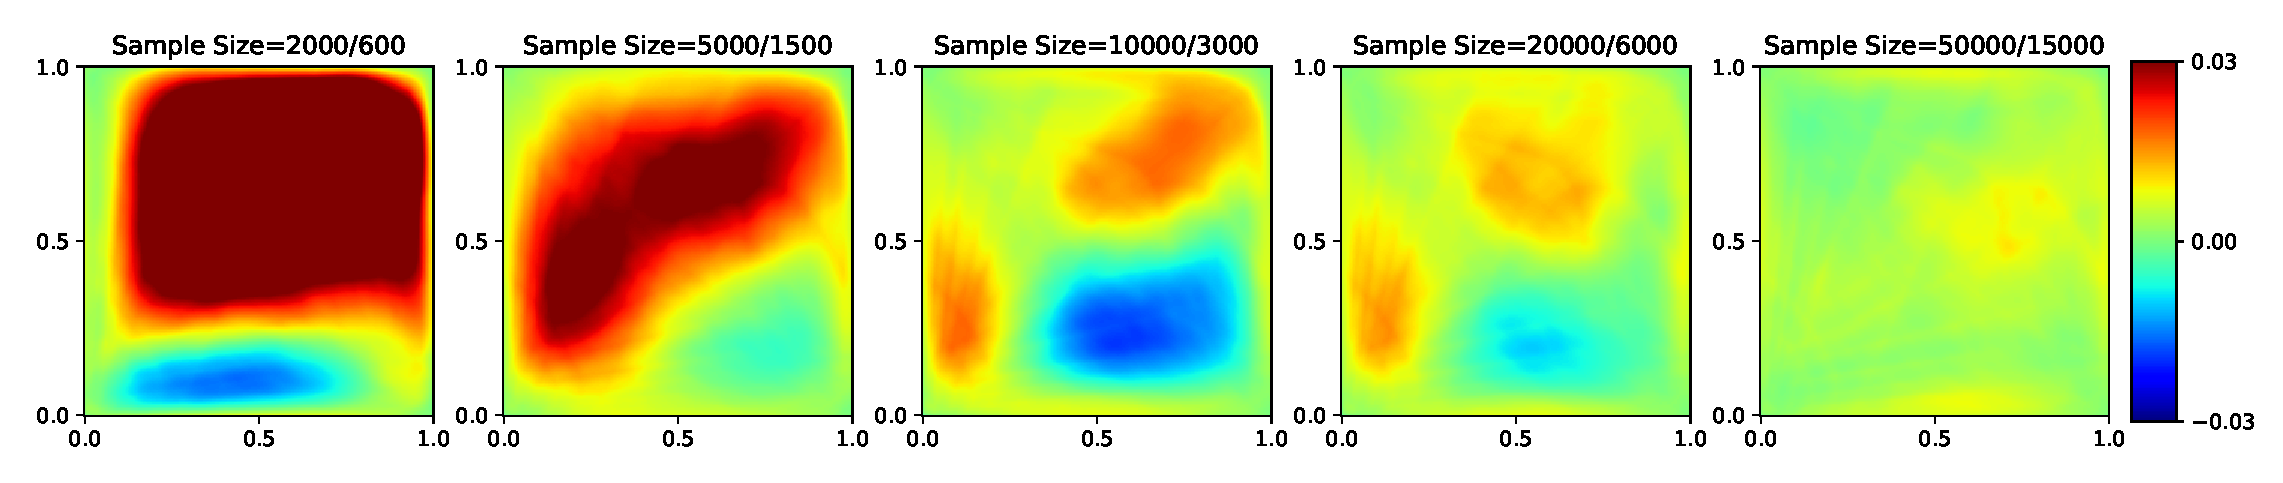
\includegraphics[width=\textwidth]{./figures2/func1_2d/HeatFig_n.eps}
    \caption{$($具有齐次边界条件的 Dirichlet 问题, $d=2)$。在不同样本量 $n$ 下，Deep Ritz 解 $u_{DRM}$ 与真解 $u_1(x)$ 之间的逐点差。} \label{fig:fig_n}
\end{figure}

\begin{figure}[htbp]
    \centering
    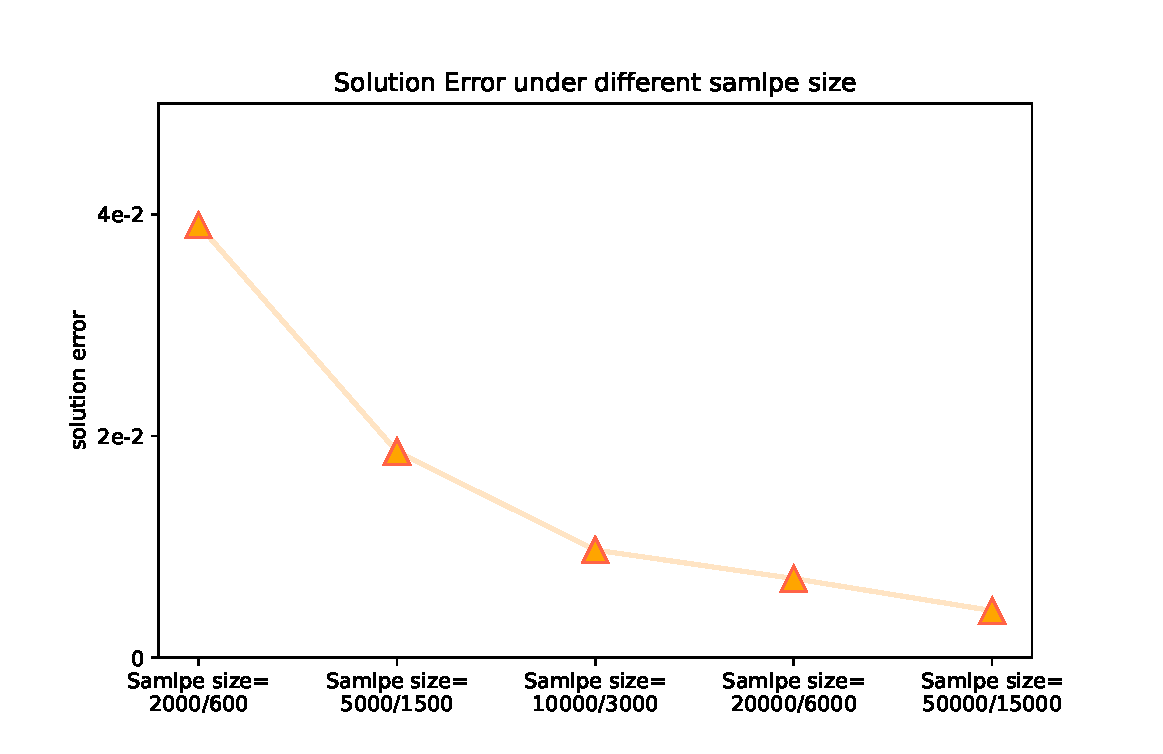
\includegraphics[width=0.5\textwidth]{./figures2/func1_2d/solution_err_under_diff_n.eps}
    \caption{$($具有齐次边界条件的 Dirichlet 问题, $d=2)$。在不同样本量 $n$ 下的 $L_2$ 解误差。} \label{fig:fig_n1}
\end{figure}

\textcolor{black}{首先，我们重点评估采样大小 $n$ 对解精度的影响。我们将网络参数设置为 $\mathcal{W} = 120$ 和 $\mathcal{D} = 4$，同时采用不同的采样大小来解决问题 \ref{eq:example1}。结果如图 \ref{fig:fig_n} 所示，且正如 图 \ref{fig:fig_n1} 中所预期的那样，较大的采样大小会导致较高的精度。这一观察结果与定理 \ref{mainthm:diri} 的结论一致。}

\textcolor{black}{值得注意的是，在上述数值实验中，我们在计算开始时仅对 $\{X_i\}_{i=1}^{n}$ 进行了一次采样。当 $n$ 较小时，算法表现不佳且收敛缓慢。为了同时提高算法的精度和效率，我们实施了一种在每个训练步或每几个训练步后对 $\{X_i\}_{i=1}^{n}$ 进行重采样的策略。这个过程类似于在无限样本集上的批量训练。通过采用这种方法，我们可以利用相对适度的计算资源有效地实现更大的 $n$，从而提高算法的泛化性能。我们的大量实验也证实了这种技术的有效性。除非另有说明，我们后续实验中提到的采样大小 $n$ 均指重采样的 $n$。}

\textcolor{black}{网络宽度 $\mathcal{W}$ 对该方法的影响如图 \ref{fig:fig_w} 和图 \ref{fig:fig_w1} 所示。我们在 $\mathcal{D} = 4$ 和 $n = 150000$ 的条件下进行了实验。实验结果表明，更宽的网络可以获得更高的精度并收敛得更快。这一发现与我们先前的结论一致。}

\begin{figure}[htbp]
    \centering
    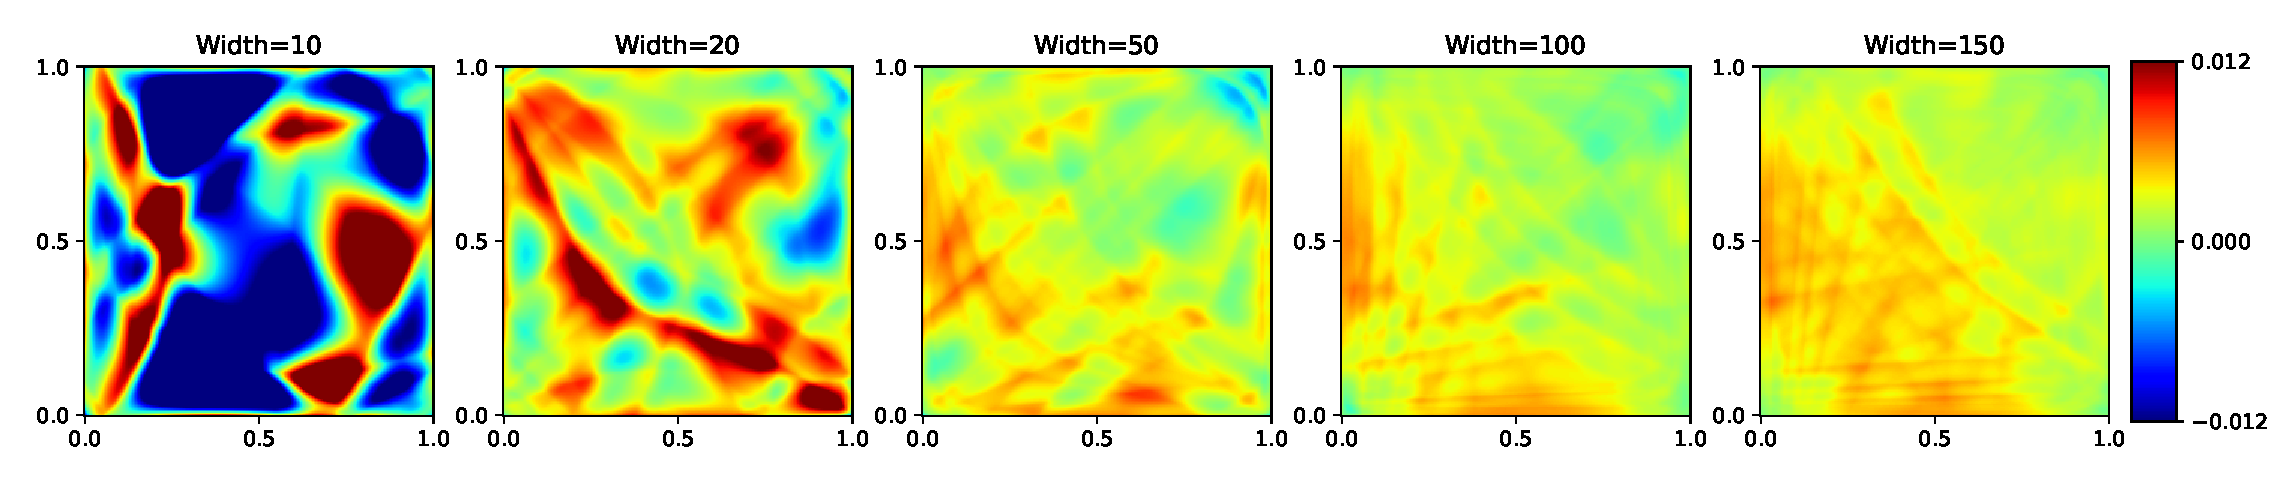
\includegraphics[width=\textwidth]{./figures2/func1_2d/HeatFig_w_5wstep.eps}
    \caption{$($具有齐次边界条件的 Dirichlet 问题， $d=2)$。在不同网络宽度 $\mathcal{W}$ 下，Deep Ritz 解 $u_{DRM}$ 与真解 $u_1(x)$ 之间的逐点差。} \label{fig:fig_w}
\end{figure}

\begin{figure}[htbp]
    \centering
    
    % --- 子图 1: L2 误差 ---
    % 建议使用 0.45\textwidth 到 0.48\textwidth
    \begin{subfigure}{0.48\textwidth}
        \centering
        % width=\linewidth 让图片自动充满子图容器(即上面的 0.48\textwidth)
        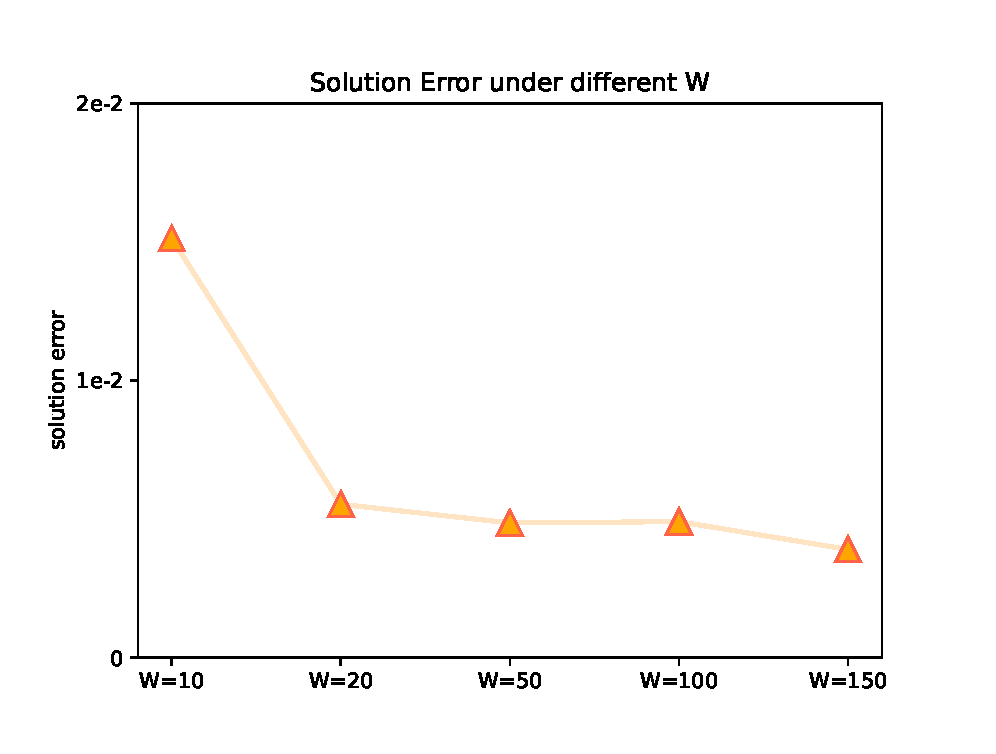
\includegraphics[width=\linewidth]{./figures2/func1_2d/solution_err_under_diff_w.eps}
        \caption{$L_2$ 解误差}
        \label{fig:l2_error_w}
    \end{subfigure}
    \hfill % 弹性间距，将两张图撑开
    % --- 子图 2: 训练误差 ---
    \begin{subfigure}{0.48\textwidth}
        \centering
        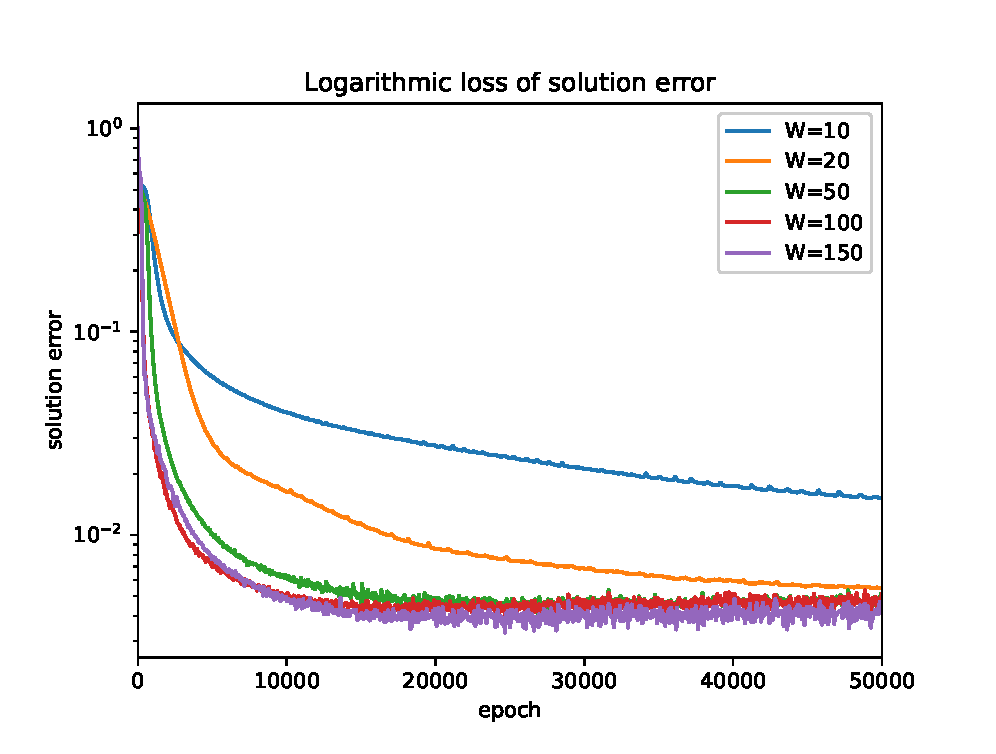
\includegraphics[width=\linewidth]{./figures2/func1_2d/Fig_w_5wstep.eps}
        \caption{训练过程中的误差}
        \label{fig:training_error_w}
    \end{subfigure}
    
    \caption{(具有齐次边界条件的 Dirichlet 问题， $d=2$)。Deep Ritz 方法在不同网络宽度 $\mathcal{W}$ 下的收敛性能。}
    \label{fig:fig_w1}
\end{figure}

\textcolor{black}{随后我们研究 $d=10$ 的情形。由于高维性以及 $S(x)$ 引入的非线性，求解该方程变得极具挑战性。传统的计算技术，如有限差分法 (FDM) 和有限元法 (FEM)，已被证明难以奏效。尽管面临这些挑战，Deep Ritz 方法依然有效，如图 \ref{fig:func1} 所示。我们在 $\Omega$ 的对角线上绘制了近似解和精确解，如图 \ref{fig:func1} (a) 所示。$L^{2}$ 误差随训练轮次的变化趋势如图 \ref{fig:func1} (b) 所示，损失函数如图 \ref{fig:func1} (c) 所示}

\textcolor{black}{该数值实验的参数配置如下：$\varepsilon=2000$，深度 $\mathcal{D}=4$，宽度 $\mathcal{W}=80$，样本量为 $200000$，边界样本量为 $80000$。我们采用 Adam 算法来最小化目标函数，初始学习率设定为 1.8e-3。采用了等间隔学习率衰减策略，其中学习率每隔 $5000$ 步衰减为原来的 $0.9$。}

\begin{figure}[htbp]
    \centering
    
    % --- 子图 1: 解的近似 ---
    \begin{subfigure}{0.32\textwidth}
        \centering
        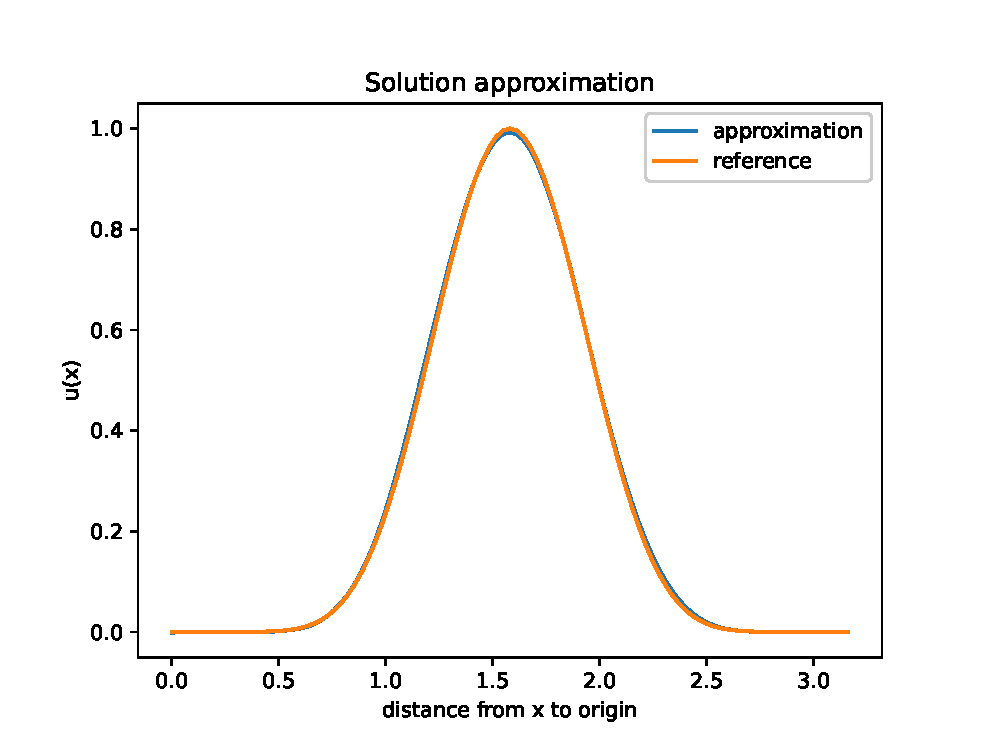
\includegraphics[width=\linewidth]{./figures2/func1/unn.eps}
        \caption{对角线上的解近似值}
        \label{fig:func1_approx}
    \end{subfigure}
    \hfill % 弹性间距
    % --- 子图 2: L2 误差 ---
    \begin{subfigure}{0.32\textwidth}
        \centering
        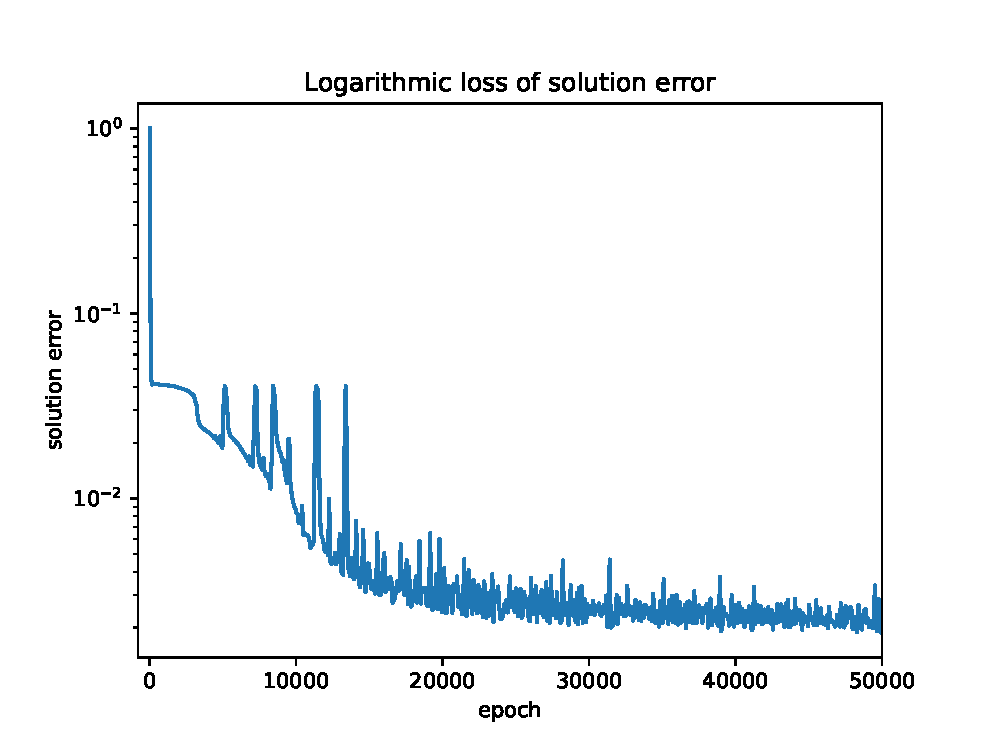
\includegraphics[width=\linewidth]{./figures2/func1/solution_err.eps}
        \caption{训练期间的 $L_2$ 误差}
        \label{fig:func1_err}
    \end{subfigure}
    \hfill % 弹性间距
    % --- 子图 3: 损失 ---
    \begin{subfigure}{0.32\textwidth}
        \centering
        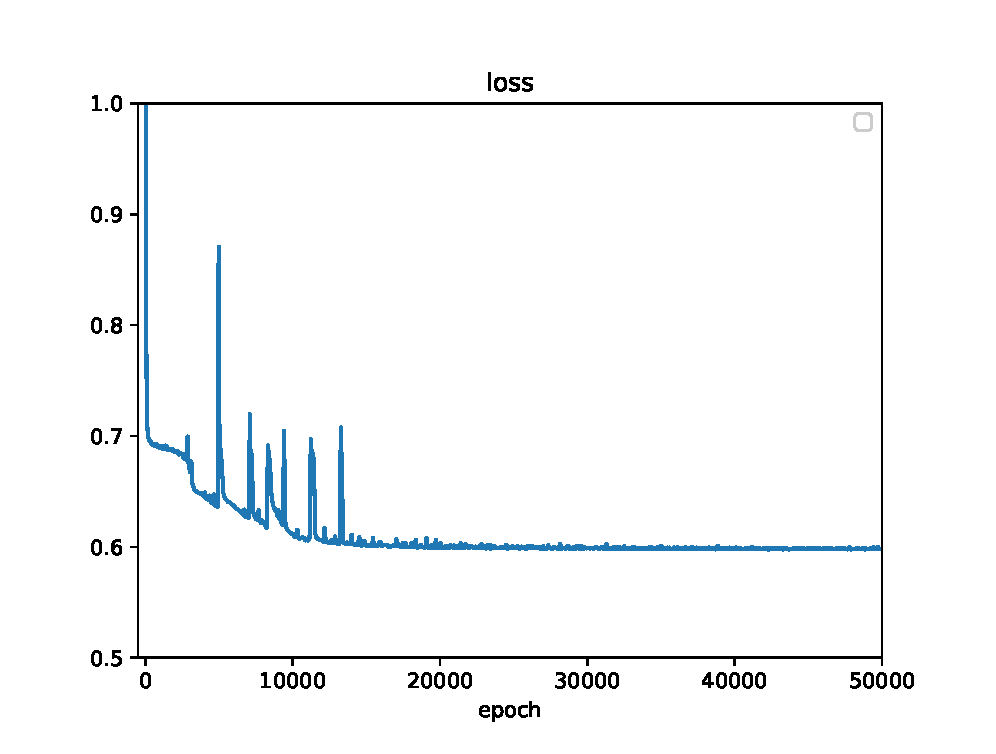
\includegraphics[width=\linewidth]{./figures2/func1/loss.eps}
        \caption{训练期间的损失函数}
        \label{fig:func1_loss}
    \end{subfigure}
    
    \caption{具有齐次边界条件的 Dirichlet 问题 ($d=10$)。由于无法直接可视化高维空间中的函数，此处展示立方体区域对角线上的值并与真实解对比。}
    \label{fig:func1}
\end{figure}


\subsection{具有非齐次边界条件的 Dirichlet 问题}
\textcolor{black}{为了说明我们理论的通用性，我们考虑以下非齐次 Dirichlet 问题。}
\begin{equation}\label{eq:example2}
\left\{\begin{aligned}
-\Delta u + S(u) & = g_2(x) & \text{在 } & \Omega \text{ 上},\\
Tu& = T g_2(x) & \text{在 } & \partial\Omega \text{ 上},\\
\end{aligned}\right.
\end{equation}

其中 $\Omega=[-1,1]^{10}$，并且
\begin{equation*}
g_2(x)=\left\{\begin{array}{lll}
\frac{2}{d} + S \left( \left(\frac{1}{d}\sum_{i=1}^{d}x_{i}\right)^{2} \right), & \left| \frac{1}{d}\sum_{i=1}^{d}x_{i} \right|> \sqrt{0.3},\\
S(0.3), & \left| \frac{1}{d}\sum_{i=1}^{d}x_{i} \right|\leq \sqrt{0.3},\\
\end{array}\right.
\end{equation*}
上述非齐次问题的解由下式给出：
\begin{equation*}
u_2(x)=\left\{\begin{array}{lll}
\left(\frac{1}{d}\sum_{i=1}^{d}x_{i}\right)^{2}, & \left| \frac{1}{d}\sum_{i=1}^{d}x_{i} \right|> \sqrt{0.3},\\
0.3, & \left| \frac{1}{d}\sum_{i=1}^{d}x_{i} \right|\leq \sqrt{0.3},\\
\end{array}\right.
\end{equation*}
与前一个方程相比，问题 \ref{eq:example2} 不仅是一个非齐次边界问题，而且涉及非光滑解。

\textcolor{black}{本次数值实验的参数配置如下：$\varepsilon=2000$，深度 $\mathcal{D}=4$，宽度 $\mathcal{W}=150$，样本量为 $150000$，边界样本量为 $40000$。其他参数与之前相同。如图 \ref{fig:func2} 所示，在此设置下，所提方法也能准确地逼近解。}

\begin{figure}[htbp]
    \centering
    
    % --- 第一张子图 ---
    % 设置宽度为 0.32 倍文本宽度，留出空隙给间距
    \begin{subfigure}{0.32\textwidth}
        \centering
        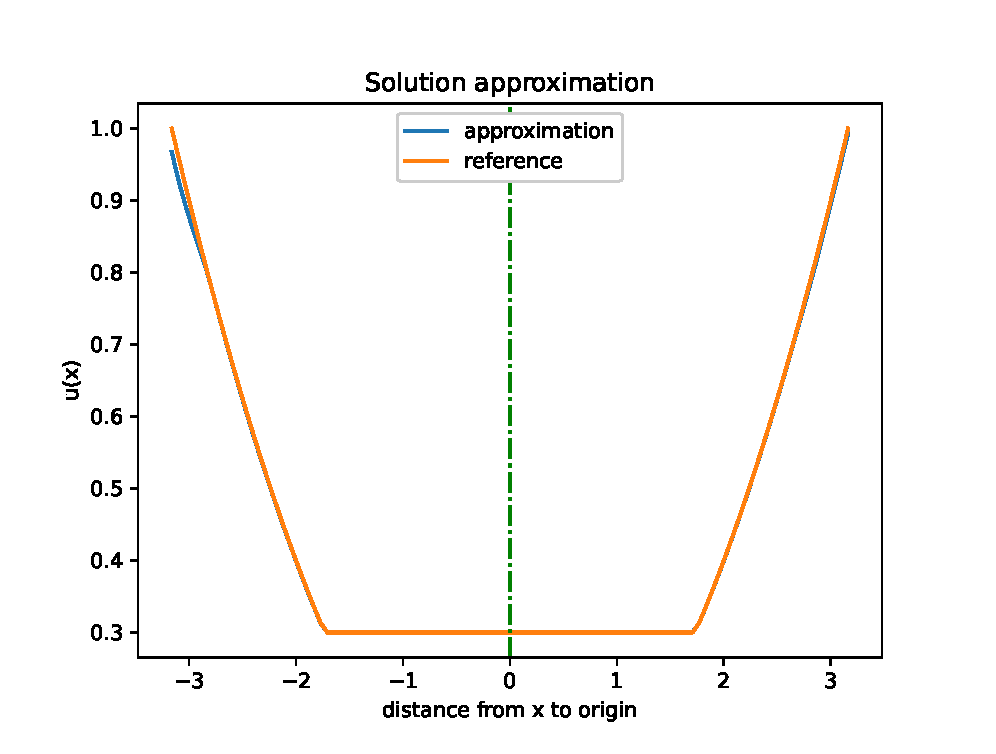
\includegraphics[width=\linewidth]{./figures2/func2/unn.eps}
        \caption{立方体区域对角线上的解逼近}
        \label{fig:func2_approx}
    \end{subfigure}
    \hfill % 弹性间距
    % --- 第二张子图 ---
    \begin{subfigure}{0.32\textwidth}
        \centering
        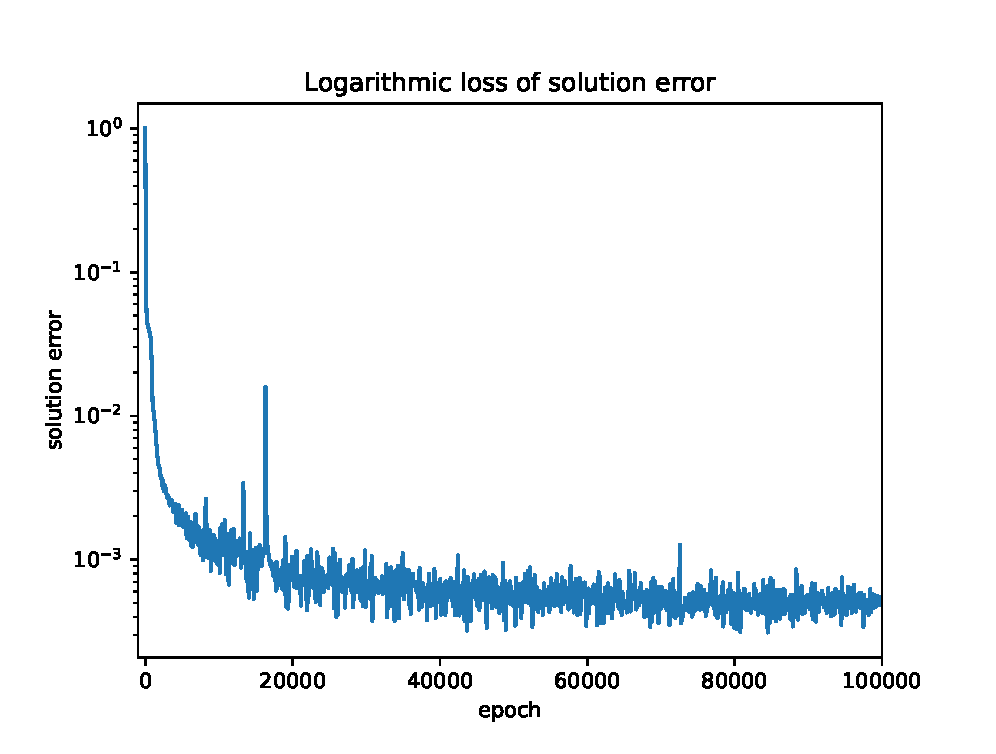
\includegraphics[width=\linewidth]{./figures2/func2/solution_err.eps}
        \caption{训练过程中的 $L_2$ 误差}
        \label{fig:func2_err}
    \end{subfigure}
    \hfill % 弹性间距
    % --- 第三张子图 ---
    \begin{subfigure}{0.32\textwidth}
        \centering
        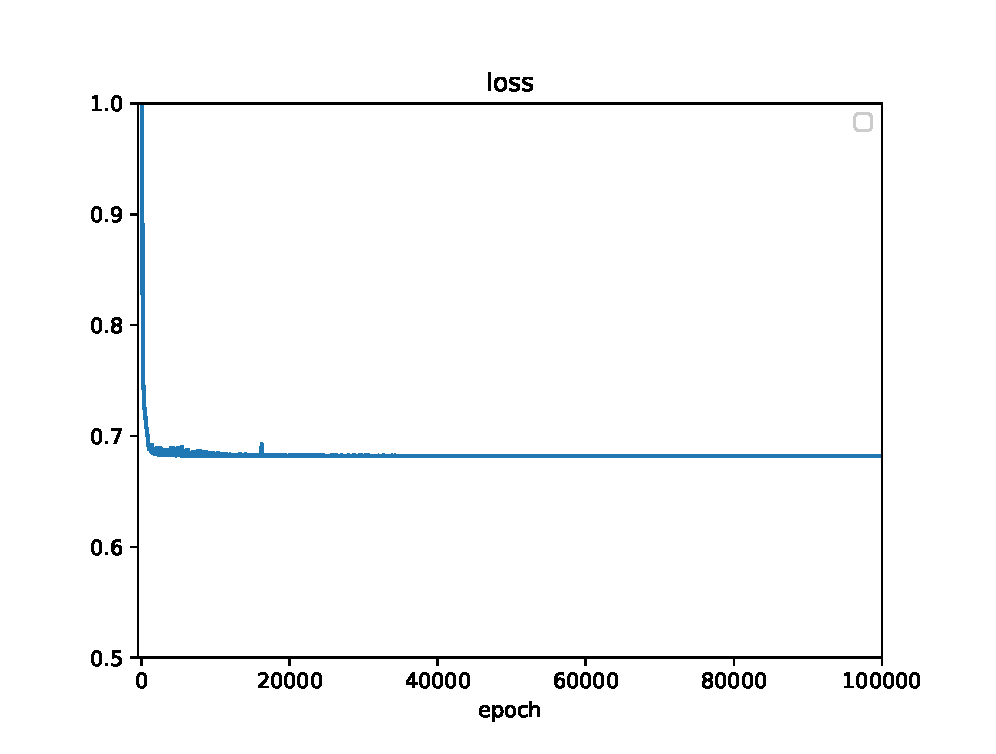
\includegraphics[width=\linewidth]{./figures2/func2/loss.eps}
        \caption{训练过程中的损失值}
        \label{fig:func2_loss}
    \end{subfigure}
    
    \caption{非齐次边界条件下的 Dirichlet 问题 ($d=10$)}
    \label{fig:func2}
\end{figure}



\section{讨论}\label{sec:dis}
在本文中，我们研究了利用具有 $\mathrm{ReLU}^2$ 激活函数的 ResNet 求解半线性椭圆问题。我们提出了一种基于惩罚变分形式的通用公式，用于计算半线性椭圆方程的解。随后，我们使用 Deep Ritz 方法对该惩罚变分形式进行求解。我们根据 $\mathrm{ReLU}^2$ ResNet 的深度 $\mathcal{D}$ 和宽度 $\mathcal{W}$ 以及训练样本数量 $n$，推导了估计解与真解之间误差的上界。我们的数值模拟结果证明了所提方法在克服维数灾难方面的有效性，并验证了我们的理论结果。

\section{附录}\label{sec:appd}
\textcolor{black}{在本附录中，我们给出了 4.3 节中引入的几个引理的完整证明。Deep Ritz 方法的统计误差分析遵循标准化流程，因此，正文中省略了这一部分。}

引理 \ref{lemma:staerr:Rad234} 的证明。
\begin{proof}\label{pf:lemma:staerr:Rad234}
我们将分两部分给出证明，每一部分都可以利用两个不同的事实单独获得。
第一个事实是 Rademacher 复杂度可以通过 Lipschitz 连续函数传递。这一事实使我们能够建立最后四个不等式：
\begin{lemma}\label{lemma:staerr:liprad}
假设 $\psi:\mathbb{R}^{d}\times\mathbb{R}\rightarrow\mathbb{R}$, $(x,y)\mapsto\psi(x,y)$ 对于所有 $x$ 在 $y$ 上是 $\ell$-Lipschitz 连续的。设 $\mathcal{N}$ 是 $\Omega$ 上的一类函数，且 $\psi\circ\mathcal{N}=\{\psi\circ u:x\mapsto\psi(x,u(x)) ,u\in\mathcal{N}\}$。那么
\begin{equation*}
\mathfrak{R}(\psi\circ\mathcal{N})\leq\ell \ \mathfrak{R}(\mathcal{N})
\end{equation*}
\end{lemma}
对于该陈述的推导，我们引用 \cite{ledoux2013probability} 中的推论 3.17。

显然，第 2、3、4 和 5 项的 Lipschitz 常数分别为 $2\|f\|_{\infty}$，$2K$，$2\varepsilon \mathcal{B}$ 和 $4\varepsilon \|h\|_{\infty}$。因此，可以以相同的方式直接得出它们的结论。

第一项需要特殊处理，因为 $\nabla$ 算子不是 Lipschitz 连续的。这一考虑直接遵循以下断言：
\par\noindent{\textbf{断言}：设 $u$ 是由深度为 $\mathcal{D}$ 且宽度为 $\mathcal{W}$ 的 $\mathrm{ReLU}^{2}$ 网络实现的函数。那么 $\|\nabla u\|_2^2$ 可以由深度为 $\mathcal{D}+3$ 且宽度为 $d\left(\mathcal{D}+2\right)\mathcal{W}$ 的 $\mathrm{ReLU}$-$\mathrm{ReLU}^{2}$ 网络实现。}

将 $\mathrm{ReLU}$ 和 $\mathrm{ReLU}^{2}$ 分别记为 $\sigma_1$ 和 $\sigma_2$。
只要我们证明每个偏导数 $D_iu(i=1,2,\cdots,d)$ 可以分别由 $\mathrm{ReLU}$-$\mathrm{ReLU}^{2}$ 网络实现，我们就可以轻松获得所需的网络，因为 $\|\nabla u\|_2^2=\sum_{i=1}^{d}\left|D_i u\right|^2$ 且平方函数可以通过 $x^2=\sigma_2(x)+\sigma_2(-x)$ 实现。
	
现在我们证明对于任何 $i=1,2,\cdots,d$，$D_iu$ 都可以由 $\mathrm{ReLU}$-$\mathrm{ReLU}^{2}$ 网络实现。我们将重点详细解释前两层，因为 $k\geq3$ 的层过程是类似的，并且可以通过归纳法推导。对于第一层，由于 $\sigma_2^{'}(x)=2\sigma_1(x)$，对于任何 $q=1,2\cdots,n_1$，我们有
\begin{equation*}
D_iu_q^{(1)}=D_i\sigma_2\left(\sum_{j=1}^{d}a_{qj}^{(1)}x_j+b_q^{(1)}\right)
=2\sigma_1\left(\sum_{j=1}^{d}a_{qj}^{(1)}x_j+b_q^{(1)}\right)\cdot a_{qi}^{(1)}
\end{equation*}
因此 $D_iu_q^{(1)}$ 可以由深度为 $2$ 宽度为 $1$ 的 $\mathrm{ReLU}$-$\mathrm{ReLU}^{2}$ 网络实现。对于第二层，
\begin{equation*}
D_iu_q^{(2)}=D_i\sigma_2\left(\sum_{j=1}^{n_1}a_{qj}^{(2)}u_j^{(1)}+b_q^{(2)}\right)
=2\sigma_1\left(\sum_{j=1}^{n_1}a_{qj}^{(2)}u_j^{(1)}+b_q^{(2)}\right)\cdot\sum_{j=1}^{n_1}a_{qj}^{(2)}D_iu_j^{(1)}.
\end{equation*}
由于 $\sigma_1\left(\sum_{j=1}^{n_1}a_{qj}^{(2)}u_j^{(1)}+b_q^{(2)}\right)$ 和 $\sum_{j=1}^{n_1}a_{qj}^{(2)}D_iu_j^{(1)}$ 可以分别由 $\mathrm{ReLU}-\mathrm{ReLU}^{2}$ 子网络实现，并且乘法也可以通过下式实现：
\begin{equation*}
\begin{split}
x\cdot y&=\frac{1}{4}\left[(x+y)^2-(x-y)^2\right]\\
&=\frac{1}{4}\left[\sigma_2(x+y)+\sigma_2(-x-y)-\sigma_2(x-y)-\sigma_2(-x+y)\right].
\end{split}
\end{equation*}
我们得出结论，$D_iu_q^{(2)}$ 可以由 $\mathrm{ReLU}$-$\mathrm{ReLU}^{2}$ 网络实现。我们有 $$\mathcal{D}\left(\sigma_1\left(\sum_{j=1}^{n_1}a_{qj}^{(2)}u_j^{(1)}+b_q^{(2)}\right)\right)=3, \mathcal{W}\left(\sigma_1\left(\sum_{j=1}^{n_1}a_{qj}^{(2)}u_j^{(1)}+b_q^{(2)}\right)\right)\leq\mathcal{W}$$ 以及 $$\mathcal{D}\left(\sum_{j=1}^{n_1}a_{qj}^{(2)}D_iu_j^{(1)}\right)=2, \mathcal{W}\left(\sum_{j=1}^{n_1}a_{qj}^{(2)}D_iu_j^{(1)}\right)\leq\mathcal{W}。$$ 因此 $\mathcal{D}\left(D_iu_q^{(2)}\right)=4,$ $\mathcal{W}\left(D_iu_q^{(2)}\right)\leq\max\{2\mathcal{W},4\}$。

现在我们对 $k\geq3$ 的层应用归纳法。对于第三层，
\begin{equation*}
D_iu_q^{(3)}=D_i\sigma_2\left(\sum_{j=1}^{n_2}a_{qj}^{(3)}u_j^{(2)}+b_q^{(3)}\right)
=2\sigma_1\left(\sum_{j=1}^{n_2}a_{qj}^{(3)}u_j^{(2)}+b_q^{(3)}\right)\cdot\sum_{j=1}^{n_2}a_{qj}^{(3)}D_iu_j^{(2)}.
\end{equation*}
由于
\begin{equation*}
\mathcal{D}\left(\sigma_1\left(\sum_{j=1}^{n_2}a_{qj}^{(3)}u_j^{(2)}+b_q^{(3)}\right)\right)=4, \mathcal{W}\left(\sigma_1\left(\sum_{j=1}^{n_2}a_{qj}^{(3)}u_j^{(2)}+b_q^{(3)}\right)\right)\leq\mathcal{W}
\end{equation*}
以及
\begin{equation*}
\mathcal{D}\left(\sum_{j=1}^{n_2}a_{qj}^{(3)}D_iu_j^{(2)}\right)=4, \mathcal{W}\left(\sum_{j=1}^{n_1}a_{qj}^{(3)}D_iu_j^{(2)}\right)\leq\max\{2\mathcal{W},4\mathcal{W}\}=4\mathcal{W},
\end{equation*}
我们得出结论，$D_iu_q^{(3)}$ 可以由 $\mathrm{ReLU}$-$\mathrm{ReLU}^{2}$ 网络实现，并且 $$\mathcal{D}\left(D_iu_q^{(3)}\right)=5, \mathcal{W}\left(D_iu_q^{(3)}\right)\leq\max\{5\mathcal{W},4\}=5\mathcal{W}。$$

我们假设 $D_iu_q^{(k)}(q=1,2,\cdots,n_k)$ 可以由 $\mathrm{ReLU}$-$\mathrm{ReLU}^{2}$ 网络实现，并且 $\mathcal{D}\left(D_iu_q^{(k)}\right)=k+2$, $\mathcal{W}\left(D_iu_q^{(3)}\right)\leq(k+2)\mathcal{W}$。对于第 $(k+1)$ 层，
\begin{align}
&D_iu_q^{(k+1)}=D_i\sigma_2\left(\sum_{j=1}^{n_k}a_{qj}^{(k+1)}u_j^{(k)}+b_q^{(k+1)}\right)\\
&=2\sigma_1\left(\sum_{j=1}^{n_k}a_{qj}^{(k+1)}u_j^{(k)}+b_q^{(k+1)}\right)\cdot\sum_{j=1}^{n_k}a_{qj}^{(k+1)}D_iu_j^{(k)}.
\end{align}
由于
\begin{equation*}
\begin{aligned}
\mathcal{D}\left(\sigma_1\left(\sum_{j=1}^{n_k}a_{qj}^{(k+1)}u_j^{(k)}+b_q^{(k+1)}\right)\right)&=k+2, \\
\mathcal{W}\left(\sigma_1\left(\sum_{j=1}^{n_k}a_{qj}^{(k+1)}u_j^{(k)}+b_q^{(k+1)}\right)\right)&\leq\mathcal{W},
\end{aligned}
\end{equation*}
以及
\begin{equation*}
\begin{aligned}
\mathcal{D}\left(\sum_{j=1}^{n_k}a_{qj}^{(k+1)}D_iu_j^{(k)}\right)&=k+2, \\ \mathcal{W}\left(\sum_{j=1}^{n_k}a_{qj}^{(k+1)}D_iu_j^{(k)}\right)&\leq\max\{(k+2)\mathcal{W},4\mathcal{W}\}=(k+2)\mathcal{W},
\end{aligned}
\end{equation*}
我们得出结论，$D_iu_q^{(k+1)}$ 可以由 $\mathrm{ReLU}$-$\mathrm{ReLU}^{2}$ 网络实现，并且 $\mathcal{D}\left(D_iu_q^{(k+1)}\right)=k+3$, $\mathcal{W}\left(D_iu_q^{(k+1)}\right)\leq\max\{(k+3)\mathcal{W},4\}=(k+3)\mathcal{W}$。
	
由此我们推导出 $D_iu=D_iu_1^{\mathcal{D}}$ 可以由 $\mathrm{ReLU}$-$\mathrm{ReLU}^{2}$ 网络实现，并且 $\mathcal{D}\left(D_iu\right)=\mathcal{D}+2$, $\mathcal{W}\left(D_iu\right)\leq\left(\mathcal{D}+2\right)\mathcal{W}$。最终，我们获得：
\begin{equation}\label{eq:N12}
    \mathcal{D}\left(\|\nabla u\|^2\right)=\mathcal{D}+3, \mathcal{W}\left(\|\nabla u\|^2\right)\leq d\left(\mathcal{D}+2\right)\mathcal{W}.
\end{equation}
\end{proof}

Proof of lemma \ref{lemma:staerr:Rad_cover}.
引理 \ref{lemma:staerr:Rad_cover} 的证明。
\begin{proof}
\label{pf:lemma:staerr:Rad_cover}
首先，我们介绍 Massart 有限类引理，其证明可以在 \cite{boucheron2013concentration} 中找到。
\begin{lemma}[Massart 有限类引理 \cite{boucheron2013concentration}]\label{Mfinite}
对于任意具有直径 $D=\sum_{v\in V}\|v\|_{2}$ 的有限集 $V\in\mathbb{R}^{n}$，有
\begin{equation*}
\mathbb{E}_{\sigma_{i}}\left[ \sup_{v\in V}\frac{1}{n}\left| \sum_{i}\sigma_{i}v_{i} \right| \right] \leq \frac{D}{n}\sqrt{2\log(2|V|)},
\end{equation*}
其中 $\{\sigma_{i}\}_{i=1}^{n}$ 是 Rademacher 变量，其定义与定义 \ref{def:staerr:radcom} 中相同。
\end{lemma}

令 $\varepsilon_{j}=2^{-k+1} B$。我们将 $\mathcal{F}_{k}$ 记为 $\mathcal{F}$ 的一个 $\varepsilon_{k}$-覆盖，且 $\left|\mathcal{F}_{k}\right|=\mathcal{C}\left(\varepsilon_{k}, \mathcal{F},\|\cdot\|_{\infty}\right) $。因此对于任意 $u \in \mathcal{F}$，存在 $u_{k} \in \mathcal{F}_{k}$ 使得 $\left\|u-u_{k}\right\|_{\infty} \leq \varepsilon_{k} $。设 $K$ 为一个稍后确定的正整数。我们有
\begin{equation*}
\begin{array}{rcl}
{}&{}&\mathbb{E}_{\left\{\sigma_{i}, Z_{i}\right\}_{i=1}^{n}}\left[\sup\limits_{u \in \mathcal{F}} \frac{1}{n}\left|\sum\limits_{i=1}^{n} \sigma_{i} u\left(Z_{i}\right)\right|\right]\\
{}&{}&{}\\
{}&=&\mathbb{E}_{\left\{\sigma_{i}, Z_{i}\right\}_{i=1}^{n}}\left[\sup\limits _{u \in \mathcal{F}} \frac{1}{n}\left|\sum\limits_{i=1}^{n} \sigma_{i}\left(u\left(Z_{i}\right)-u_{K}\left(Z_{i}\right)\right)\right.\right.\\
{}&{}&\left.\left.+\sum\limits_{j=1}^{K-1} \sum\limits_{i=1}^{n} \sigma_{i}\left(u_{j+1}\left(Z_{i}\right)-u_{j}\left(Z_{i}\right)\right)+\sum\limits_{i=1}^{n} \sigma_{i} u_{1}\left(Z_{i}\right)\right|\right]\\
{}&{}&{}\\
{}&\leq&\mathbb{E}_{\left\{\sigma_{i}, Z_{i}\right\}_{i=1}^{n}}\left[\sup\limits _{u \in \mathcal{F}} \frac{1}{n}\left|\sum\limits_{i=1}^{n} \sigma_{i}\left(u\left(Z_{i}\right)-u_{K}\left(Z_{i}\right)\right)\right|\right]\\
{}&{}&+\sum\limits_{j=1}^{K-1} \mathbb{E}_{\left\{\sigma_{i}, Z_{t}\right\}_{i=1}^{n}}\left[\sup\limits _{u \in \mathcal{F}} \frac{1}{n}\left|\sum\limits_{i=1}^{n} \sigma_{i}\left(u_{j+1}\left(Z_{i}\right)-u_{j}\left(Z_{i}\right)\right)\right|\right]\\
{}&{}&+\mathbb{E}_{\left\{\sigma_{i}, Z_{t}\right\}_{k=1}^{n}}\left[\sup\limits _{u \in \mathcal{F}} \frac{1}{n}\left|\sum\limits_{i=1}^{n} \sigma_{i} u_{1}\left(Z_{i}\right)\right|\right]
\end{array}
\end{equation*}
由于 $0 \in \mathcal{F}$，我们可以选择 $\mathcal{F}_{1}=\{0\}$ 来消去第三项。对于第一项，
\begin{equation*}
\begin{array}{rcl}
{}&{}&\mathbb{E}_{\left\{\sigma_{i}, Z_{i}\right\}_{t=1}^{n}}\left[\sup\limits _{u \in \mathcal{F}} \frac{1}{n}\left|\sum\limits_{i=1}^{n} \sigma_{i}\left(u\left(Z_{i}\right)-u_{K}\left(Z_{i}\right)\right)\right|\right]\\
{}&\leq&\mathbb{E}_{\left\{\sigma_{i}, Z_{i}\right\}_{i=1}^{n}}\left[\sup\limits _{u \in \mathcal{F}} \frac{1}{n} \sum\limits_{i=1}^{n}\left|\sigma_{i}\right|\left\|u-u_{K}\right\|_{\infty}\right] \leq \varepsilon_{K}
\end{array}
\end{equation*}
对于第二项，定义 $v_{i}^{j}=u_{j+1}\left(Z_{i}\right)-u_{j}\left(Z_{i}\right)$，并应用引理 \ref{Mfinite}，我们有
\begin{equation*}
\begin{aligned}
&\sum_{j=1}^{K-1} \mathbb{E}_{\{\sigma\}_{i=1}^{n}}\left[\sup _{u \in \mathcal{F}} \frac{1}{n}\left|\sum_{i=1}^{n} \sigma_{i}\left(u_{j+1}\left(Z_{i}\right)-u_{j}\left(Z_{i}\right)\right)\right|\right]                                              \\
=&\sum_{j=1}^{K-1} \mathbb{E}_{\left\{\sigma_{t}\right\}_{t=1}^{n}}\left[\sup _{v \in V_{j}} \frac{1}{n} \left| \sum_{i=1}^{n} \sigma_{i} v_{i}^{j}\right|\right] \leq \sum_{j=1}^{K-1} \frac{D_{j}}{n} \sqrt{2 \log \left(2\left|V_{j}\right|\right)}.
\end{aligned}
\end{equation*}
根据 $V_{j}$ 的定义，我们可知 $\left|V_{j}\right| \leq\left|\mathcal{F}_{j}\right|\left|\mathcal{F}_{j+1}\right| \leq\left|\mathcal{F}_{j+1}\right|^{2}$ 并且
\begin{equation*}
\begin{aligned}
\|V\|_{2} & =\left(\sum_{i=1}^{n}\left|u_{j+1}\left(Z_{i}\right)-u_{j}\left(Z_{i}\right)\right|^{2}\right)^{1 / 2} \leq \sqrt{n}\left\|u_{j+1}-u_{j}\right\|_{\infty}\\
&\leq \sqrt{n}\left\|u_{j+1}-u\right\|_{\infty}+\sqrt{n}\left\|u_{j}-u\right\|_{\infty}=\sqrt{n} \varepsilon_{j+1}+\sqrt{n} \varepsilon_{j}=3 \sqrt{n} \varepsilon_{j+1}.
\end{aligned}
\end{equation*}
因此
\begin{equation*}
\begin{aligned}
&\sum_{j=1}^{K-1} \mathbb{E}_{\left\{\sigma_{i}, Z_{t}\right\}_{t=1}^{n}}\left[\sup _{u \in \mathcal{F}} \frac{1}{n}\left|\sum_{i=1}^{n} \sigma_{i}\left(u_{j+1}\left(Z_{i}\right)-u_{j}\left(Z_{i}\right)\right)\right|\right] \\
&\leq \sum_{j=1}^{K-1} \frac{D_{j}}{n} \sqrt{2 \log \left(2\left|V_{j}\right|\right)} \leq \sum_{j=1}^{K-1} \frac{3 \varepsilon_{j+1}}{\sqrt{n}} \sqrt{2 \log \left(2\left|\mathcal{F}_{j+1}\right|^{2}\right)}
\end{aligned}
\end{equation*}
现在我们得到
\begin{equation*}
\begin{aligned}
&\mathbb{E}_{\left\{\sigma_{i}, Z_{i}\right\}_{i=1}^{n}}\left[\sup _{u \in \mathcal{F}} \frac{1}{n}\left|\sum_{i=1}^{n} \sigma_{i} u\left(Z_{i}\right)\right|\right] \leq \varepsilon_{K}+\sum_{j=1}^{K-1} \frac{6 \varepsilon_{j+2}}{\sqrt{n}} \sqrt{2 \log \left(2\left|\mathcal{F}_{j+1}\right|^{2}\right)} \\
&=\varepsilon_{K}+\frac{6}{\sqrt{n}} \sum_{j=1}^{K-1}\left(\varepsilon_{j+1}-\varepsilon_{j+2}\right) \sqrt{2 \log \left(2 \mathcal{C}\left(\varepsilon_{j+1}, \mathcal{F},\|\cdot\|_{\infty}\right)^{2}\right)}                                                                                                     \\
&\leq \varepsilon_{K}+\frac{6}{\sqrt{n}} \int_{\varepsilon_{K+1}}^{B / 2} \sqrt{2 \log \left(2 \mathcal{C}\left(\varepsilon, \mathcal{F},\|\cdot\|_{\infty}\right)^{2}\right)} d \varepsilon.
\end{aligned}
\end{equation*}
通过对于任意 $0<\delta<\frac{B}{2}$ 选择合适的 $K$ 使得 $\varepsilon_{K+2}<\delta \leq \varepsilon_{K+1}$，引理得证。
\end{proof}

引理 \ref{lemma:staerr:pdim} 的证明。
\begin{proof}
\label{pf:lemma:staerr:pdim}
证明概要如下：首先，引入 $VCdim$ 和伪打散 (pseudo-shattering) 作为 $Pdim$ 的下界；然后，通过 \cite{anthony2009neural} 中的一个引理估计多项式的 $VCdim$；基于上述结论，通过类似于 \cite{bartlett2019nearly} 中定理 6 的推导来完成证明。

以下是伪打散和 $VCdim$ 的定义。
\begin{definition}
令 $\mathcal{N}$ 为从 $X=\Omega(\partial \Omega)$ 到 $\{0,1\}$ 的函数集。假设 $S=\left\{x_{1}, x_{2}, \cdots, x_{n}\right\} \subset X$。如果对于任意 $b \in\{0,1\}^{n}$，存在一个 $u \in \mathcal{N}$ 满足
\begin{equation*}
u\left(x_{i}\right)=b_{i}, \quad i=1,2, \ldots, n,
\end{equation*}
则称 $S$ 被 $\mathcal{N}$ 打散 (shattered)。
\end{definition}

\begin{definition}
$\mathcal{N}$ 的 VC 维，记为 $\operatorname{VCdim}(\mathcal{N})$，定义为被 $\mathcal{N}$ 打散的所有集合中的最大基数。
\end{definition}

引入引理 \ref{lemma:covering_number} 来估计多项式的 $Pdim$。证明可以在 \cite{anthony2009neural} 的定理 8.3 中找到。
\begin{lemma}\label{lemma:covering_number}
令 $p_1,\cdots,p_m$ 为具有 $n$ 个变量且次数不超过 $d$ 的多项式。如果 $n\leq m$，则
\begin{equation*}
|\{(\operatorname{sign}(p_1(x)),\cdots,\operatorname{sign}(p_m(x))):x\in\mathbb{R}^n\}| \leq 2\left(\frac{2emd}{n}\right)^n.
\end{equation*}
\end{lemma}

该论证遵循 \cite{bartlett2019nearly} 中定理 6 的证明。此处陈述的结果比 \cite{bartlett2019nearly} 中的定理 6 略强，因为 $\mathrm{VCdim}(\operatorname{sign}(\mathcal{N}))\leq \mathrm{Pdim}(\mathcal{N})$。

我们考虑一个新的函数集：
\begin{equation*}
\mathcal{\widetilde{N}}=\{\widetilde{u}(x,y)=\operatorname{sign}(u(x)-y): u\in\mathcal{N}\},
\end{equation*}
显然 $\mathrm{Pdim}(\mathcal{N})\leq\mathrm{VCdim}(\mathcal{\widetilde{N}})$。我们现在界定 $\mathcal{\widetilde{N}}$ 的 VC 维。记 $\mathcal{M}$ 为实现 $\mathcal{N}$ 中函数的神经网络中的参数（权重和偏置）总数，我们的目标是针对所有 $\{x_i\}_{i=1}^{m}\subset X$ 和 $\{y_i\}_{i=1}^{m}\subset\mathbb{R}$，推导出
\begin{equation*}
K_{\{x_i\},\{y_i\}}(m):=|\{(\operatorname{sign}(u(x_{1}, a)-y_1), \ldots, \operatorname{sign}(u(x_{m}, a)-y_m)): a \in \mathbb{R}^{\mathcal{M}}\}|
\end{equation*}
的一致上界。实际上，$K_{\{x_i\},\{y_i\}}(m)$ 在所有 $\{x_i\}_{i=1}^{m}\subset X$ 和 $\{y_i\}_{i=1}^{m}\subset\mathbb{R}$ 上的最大值即为增长函数 $\mathcal{G}_{\mathcal{\widetilde{N}}}(m)$。

为了应用引理 \ref{lemma:covering_number}，我们将参数空间 $\mathbb{R}^{\mathcal{M}}$ 划分为若干子集，以确保在每个子集中 $u(x_i,a)-y_i$ 是关于 $a$ 的无断点多项式。事实上，我们的划分与 \cite{bartlett2019nearly} 中的划分相同。将该划分记为 $\{P_1,P_2,\cdots,P_N\}$，其中整数 $N$ 满足
\begin{equation} \label{pdimb1}
N\leq\prod_{i=1}^{\mathcal{D}-1}2\left(\frac{2emk_i(1+(i-1)2^{i-1})}{\mathcal{M}_i}\right)^{\mathcal{M}_i}
\end{equation}
其中 $k_i$ 和 $\mathcal{M}_i$ 分别表示实现 $\mathcal{N}$ 中函数的神经网络第 $i$ 层的单元数，以及截至第 $i$ 层（含）的所有层单元输入的参数总数。关于划分的构造，请参见 \cite{bartlett2019nearly}。显然我们有
\begin{equation} \label{pdimb2}
K_{\{x_i\},\{y_i\}}(m)\leq\sum_{i=1}^{N}|\{(\operatorname{sign}(u(x_{1}, a)-y_1), \cdots, \operatorname{sign}(u(x_{m}, a)-y_m)): a\in P_i\}|
\end{equation}
注意到 $u(x_i,a)-y_i$ 是关于 $a$ 的多项式，其次数与 $u(x_i,a)$ 的次数相同，即 $1 + (\mathcal{D}-1)2^{\mathcal{D}-1}$，如 \cite{bartlett2019nearly} 所示。因此，根据引理 \ref{lemma:covering_number}，我们有
\begin{align}
& |\{(\operatorname{sign}(u(x_{1}, a)-y_1), \cdots, \operatorname{sign}(u(x_{m}, a)-y_m)): a\in P_i\}|\nonumber                          \\
& \leq2\left(\frac{2em(1+(\mathcal{D}-1)2^{\mathcal{D}-1})}{\mathcal{M}_{\mathcal{D}}}\right)^{\mathcal{M}_{\mathcal{D}}}\label{pdimb3}.
\end{align}
结合 (Eq.~\eqref{pdimb1})，(Eq.~\eqref{pdimb2})，(Eq.~\eqref{pdimb3}) 可得
\begin{equation*}
K_{\{x_i\},\{y_i\}}(m)\leq\prod_{i=1}^{\mathcal{D}}2\left(\frac{2emk_i(1+(i-1)2^{i-1})}{\mathcal{M}_i}\right)^{\mathcal{M}_i}.
\end{equation*}
随之我们有
\begin{equation*}
\mathcal{G}_{\mathcal{\widetilde{N}}}(m)\leq\prod_{i=1}^{\mathcal{D}}2\left(\frac{2emk_i(1+(i-1)2^{i-1})}{\mathcal{M}_i}\right)^{\mathcal{M}_i},
\end{equation*}
因为 $K_{\{x_i\},\{y_i\}}(m)$ 在所有 $\{x_i\}_{i=1}^{m}\subset X$ 和 $\{y_i\}_{i=1}^{m}\subset\mathbb{R}$ 上的最大值是增长函数 $\mathcal{G}_{\mathcal{\widetilde{N}}}(m)$。使用与 \cite{bartlett2019nearly} 中定理 6 证明相同的代数推导，我们获得
\begin{equation*}
\mathrm{Pdim}(\mathcal{N})\leq C\left(\mathcal{D}^2\mathcal{W}^2 \log \mathcal{U}+\mathcal{D}^3\mathcal{W}^2\right)
\leq C\left(\mathcal{D}^2\mathcal{W}^2\left( \mathcal{D}+\log \mathcal{W}\right)\right)
\end{equation*}
其中 $\mathcal{U}$ 指的是实现 $\mathcal{N}$ 中函数的神经网络的单元数。
\end{proof}
%%%%==========================================================%%%

\chapter{物理信息驱动的神经网络方法求解反势能问题}
在前一章中，我们详细探讨了利用深度里兹法（Deep Ritz Method）求解正向的椭圆型多特征值问题。沿着偏微分方程数值解的脉络，本章将视点转向一类更具挑战性、且在实际工程中极为重要的逆问题（Inverse Problems）：即在已知部分边界或内部测量数据的前提下，反向推演系统方程中的未知物理参数。具体而言，我们将提出并分析一种基于物理信息神经网络（PINNs）结合 Tikhonov 正则化的高效求解框架，用于重构椭圆方程中的未知势函数。
\section{预备知识与记号}
\subsection{问题背景与物理意义}

本文所研究的带有未知势函数的椭圆型偏微分方程在自然科学与工程领域具有极其广泛的物理背景。在宏观尺度上，此类方程常用于描述与时间无关的扩散现象或稳态热传导过程。例如，在定态扩散方程中 \cite{Bal2010Inverse}，未知的势函数通常对应于介质中的吸收（或反应）系数；而在稳态热传导模型中，它则代表了材料内部的辐射系数 \cite{Chen2020Convergence}。在微观尺度上，该类方程在形式上等价于定态薛定谔（Schrödinger）方程，用于描述微观粒子在特定势场中的量子态行为，此时未知项即对应于系统所处的势能分布。

在上述实际应用场景中，系统的内部参数（即势函数）往往无法被直接观测或先验给定。相反，我们通常只能通过传感器获取整个物理区域内部或其边界上的状态变量（如温度、浓度、波函数幅值等）的含噪测量值。因此，如何从这些不完全且带有噪声的观测数据中稳定、高精度地反演重构出真实的势函数，构成了典型的反问题。这类反势能问题在医学成像（如光学相干断层扫描）、地球物理勘探以及材料无损检测等领域具有不可替代的核心应用价值。

\subsection{数学描述与问题假设}
基于上述物理背景，我们将该反问题抽象为如下数学模型。我们考虑如下带有 Neumann 边界条件的椭圆型边值问题：
\begin{equation}\label{eq:pde:potential}
\left\{
\begin{aligned}
-\nabla\cdot(\alpha\nabla u)+Vu&=g, \quad \text{在}~\Omega~\text{中},\\
\alpha&=h, \quad \text{在}~\partial\Omega~\text{上},
\end{aligned}
\right.
\end{equation}
其中，$\Omega \subset \mathbb{R}^{d}$ 是给定的物理区域，$\alpha$ 为传导系数，$g$ 为内部源项，$h$ 为边界通量，$\partial_{\nu}$ 表示沿单位外法向量的导数。
给定一个确定的势函数 $V \in \mathcal{K}$，根据经典的椭圆偏微分方程理论 \cite{evans2010partial}，方程 \eqref{eq:pde:potential} 存在唯一的弱解 $u_V\in H^{1}(\Omega)$。基于此，我们可以良定义一个从参数空间到状态空间的非线性正演算子（Forward Operator）：
$$\mathcal{F}: V \mapsto u_V$$
为确保偏微分方程的适定性（Well-posedness）以及后续反问题理论分析的严密性，我们对计算区域和已知函数提出如下基本假设：

\begin{assumption}[正则性与有界性假设]\label{ass:tikpinn}
假设区域 $\Omega$ 和方程参数满足如下条件：
\begin{enumerate}
\item[(a)] 区域 $\Omega\subset\mathbb{R}^{d}$ ($d\geq1$) 为具有足够光滑边界 $\partial\Omega$ 的有界连通区域。传导系数 $\alpha\in C^{1}(\bar{\Omega})$，且满足一致椭圆条件：即存在常数 $\alpha_0>0$，使得对所有 $x\in\bar{\Omega}$ 均有 $\alpha(x)\geq\alpha_0$ 成立。
\item[(b)] 源密度函数满足 $g\in L^{2}(\Omega)$，边界通量函数满足 $h\in L^{2}(\partial\Omega)$。
\item[(c)] 真实的势函数 $V$ 属于如下有界容许集（Admissible Set）：
\begin{equation}\label{eq:box}
\mathcal{K}=\{V\in L^{\infty}(\Omega):0\leq\underline{V}\leq V(x)\leq\overline{V}<\infty,~\text{a.e. } x\in\Omega\},
\end{equation}
其中常数 $\underline{V}$ 和 $\overline{V}$ 分别代表容许势函数 $V(x)$ 的先验全局下界和上界。
\end{enumerate}
\end{assumption}

在反问题的设定下，我们的目标是利用状态变量 $u$ 的观测数据来重构真实的势函数 $V^\dagger \in \mathcal{K}$。在现实物理实验中，传感器采集的数据不可避免地会受到噪声污染。在整篇文章中，我们假设含噪测量数据服从如下标准的高斯加性噪声模型：
\begin{equation}\label{eq:measurement}
\left\{
\begin{array}{rcll}
u^{\delta}(x)&=&\mathcal{F}(V^{\dagger})(x)+\varepsilon_{\calI}(x),\quad &\varepsilon_{\calI}(x)\sim N(0,\delta^{2}),\quad x\in\Omega, \\ 
Tu^{\delta}(x)&=&T\mathcal{F}(V^{\dagger})(x)+\varepsilon_{\calB}(x),\quad &\varepsilon_{\calB}(x)\sim N(0,\delta^{2}),\quad x\in\partial\Omega,
\end{array}
\right.
\end{equation}
其中，$\delta > 0$ 表示噪声水平（Noise Level），$T$ 是经典的边界迹算子（Trace Operator）。基于上述统计模型，在 $L^2$ 范数意义下，含噪数据与真实状态之间满足如下确定性误差估计：

$$\|u^{\delta}-\mathcal{F}(V^{\dagger})\|_{L^{2}(\Omega)}=|\Omega|^{1/2}\delta, \quad \|Tu^{\delta}-T\mathcal{F}(V^{\dagger})\|_{L^{2}(\partial\Omega)}=|\partial\Omega|^{1/2}\delta.$$

\section{重构方法：Tikhonov-PINNs}\label{sec:tikpinns}
基于前述的数学模型，反问题的核心在于寻找一个势函数 $V$，使得其对应的系统正向响应 $u_V = \mathcal{F}(V)$ 尽可能逼近实际的测量数据。为此，我们首先定义如下的数据失配项（Data Mismatch）或测量误差泛函：
\begin{equation}\label{eq:data_mismatch}
\begin{aligned}
    \mathcal{M}(V) &= \|u^{\delta}-u_V\|_{L^{2}(\Omega)}^{2}+\|Tu^{\delta}-Tu_V\|_{L^{2}(\partial\Omega)}^{2} \\
    &= \|u^{\delta}-\mathcal{F}(V)\|_{L^{2}(\Omega)}^{2}+\|Tu^{\delta}-T\mathcal{F}(V)\|_{L^{2}(\partial\Omega)}^{2}
\end{aligned}
\end{equation}
给定公式 \eqref{eq:measurement} 中的观测数据，求解反问题等价于在满足控制方程 \eqref{eq:pde:potential} 的硬约束下，极小化上述测量误差 $\mathcal{M}(V)$。

然而，从算子理论的视角来看，给定右端项 $f \in L^2(\Omega)$，由经典的椭圆正则性理论可知，系统的弱解不仅存在且满足 $u \in H^2(\Omega)$。进一步，根据 Rellich-Kondrachov 定理，对于具有光滑边界的有界区域 $\Omega$，索伯列夫空间 $H^2(\Omega)$ 到观测空间 $L^2(\Omega)$ 的嵌入是紧的（Compact Embedding）。因此，从参数空间到观测空间的正演算子 $\mathcal{F}: V \mapsto u$ 本质上是一个紧算子，紧算子的核心特征在于其具有强烈的”积分平滑效应”，即势函数 $V$ 中的高频微扰在正向映射过程中会被极大地衰减。根据泛函分析理论，无限维空间中紧算子的逆算子必然是无界的，这意味着该反问题是高度病态的（Ill-posed）。在实际观测中，数据 $u^\delta$ 必然包含微小的随机噪声（如高频扰动）。由于逆过程会对高频分量产生极端的放大作用，若直接进行无约束或纯残差驱动的拟合，即使是极微小的测量误差也会引发灾难性的“噪声爆炸”，导致重构的势函数产生非物理的剧烈震荡。

为了克服这一不稳定性，我们在目标泛函中引入经典的 Tikhonov 正则化项，，不仅是为了平滑神经网络的损失曲面，更是恢复反问题适定性（Well-posedness）的数学必然要求。通过对势函数的一阶导数（梯度）和二阶导数（曲率）施加强烈惩罚，正则化项显式地压制了高频震荡，迫使算法在容许空间 $\mathcal{K}$ 中寻找与观测数据相容且具备物理光滑性的解。将其转化为如下的偏微分方程约束优化控制问题（PDE-constrained Optimization）：

\begin{align*}
&\min_{V,u}\quad\mathcal{J}_{\lambda}(V,u)=\|z^{\delta}-u\|_{L^{2}(\Omega)}^{2}+\|Tz^{\delta}-Tu\|_{L^{2}(\partial\Omega)}^{2}+\lambda\|V\|_{H^{2}(\Omega)}^{2}, \\
&\subto\quad Eq.\eqref{eq:pde:potential}~\text{and}~Eq.\eqref{eq:box}.
\end{align*}

其中，正则化参数 $\lambda > 0$ 用于平衡数据拟合度与解的光滑性。

传统的伴随方法（Adjoint Method）求解此类约束优化问题往往需要反复进行正向和伴随方程的网格离散与迭代求解，计算成本高昂且对复杂几何区域适应性较弱。在此，我们引入物理信息神经网络（PINNs）的“软约束”思想，通过将偏微分方程及其边界条件作为惩罚项（Penalty Terms）加入到目标函数中，从而将上述带有 PDE 约束的优化问题优雅地松弛为无约束优化问题：
\begin{equation}\label{eq:pinns:loss}
\min_{V,u} \{ \mathcal{L}_{\lambda}(V,u) = \mathcal{M}(u)+\mathcal{I}(V,u)+\mathcal{B}(u) +\mathcal{R}(V)\},
\end{equation}
其中，内部 PDE 残差惩罚项 $\mathcal{I}(V,u)$ 和边界条件残差惩罚项 $\mathcal{B}(u)$ 分别定义为：
\begin{equation*}
\mathcal{I}(V,u)=\|\nabla\cdot(\alpha\nabla u)-Vu+f\|_{L^{2}(\Omega)}^{2}, \quad \text{且} \quad
\mathcal{B}(V,u)=\|\alpha\frac{\partial u}{\partial n}-g\|_{L^{2}(\partial\Omega)}^{2}.
\end{equation*}
与标准 PINNs 框架直接利用纯数据驱动加物理残差进行优化不同，我们在损失函数 \eqref{eq:pinns:loss} 中显式保留了 Tikhonov 正则化项 $\lambda\|V\|_{H^{2}(\Omega)}^{2}$。这一微小但关键的调整构成了本文 Tikhonov-PINNs 方法的核心。正如我们在后续理论分析中所将严格证明的，该正则化项不仅能够有效抑制测量噪声的放大，而且是建立重构势函数 $V$ 严密收敛性理论（即稳定性估计）的必要前提。

基于前文（注记 \ref{remark:ill_posedness}）关于正则化必要性的探讨，本节将严格建立重构势函数 $V$ 的收敛性理论。这一理论在反问题文献中通常被称为稳定性估计（Stability Estimate）。它从数学上保证了：当我们的神经网络将损失函数优化到足够小，且测量噪声趋于零时，重构出的解能够稳定地收敛于真实解。

为了推导这一结果，我们需要对真实的势函数 $V^\dagger$ 和对应的真实状态变量 $u^\dagger$ 施加如下的正则性假设：

\begin{assumption}[真实解的正则性]\label{ass:potential:Vdaggerreg}
令 $s \in \mathbb{N}_+$，我们假设真实的势函数满足 $V^\dagger \in W^{2,\infty}(\Omega) \cap H^{s+3}(\Omega) \cap \mathcal{K}$，且对应的真实状态变量满足 $u^\dagger \in W^{2,\infty}(\Omega) \cap H^{s+3}(\Omega)$。
\end{assumption}

\begin{theorem}[稳定性估计]\label{th:potential:stability}
在方程 \eqref{eq:pde:potential} 和测量数据模型 \eqref{eq:measurement} 的设定下，令 $(V^{\dagger},u^{\dagger})$ 为满足原偏微分方程的真实物理状态对。假设 Assumption \ref{ass:potential:Vdaggerreg} 成立，假设我们不仅在区域内部获得了带噪测量 $u^\delta$，在边界上也获得了带噪测量 $g^\delta$（或边界迹 $Tu^\delta$），且满足 $\|u^\dagger - u^\delta\|_{L^2(\Omega)} + \|Tu^\dagger - Tu^\delta\|_{L^2(\partial\Omega)} \leq \delta$。则对于优化过程中任意一对满足 $V\in H^{2}(\Omega)$ 和 $u \in H^1(\Omega)$ 的参数对 $(V,u)$，如下误差估计成立：
\begin{equation*}
\|(V-V^{\dagger})u^{\dagger}\|_{L^{2}(\Omega)} \leq C\left(1+\lambda^{-1/4}\mathcal{L}_{\lambda}^{1/4}(V,u)\right)\left(\mathcal{L}_{\lambda}^{1/4}(V,u)+\delta^{1/2}\right),
\end{equation*}
其中 $C$ 是一个严格依赖于区域维数 $d$、区域形状 $\Omega$、传导系数 $\alpha$、容许集上界 $\overline{V}$，以及真实解范数 $\|V^{\dagger}\|_{W^{2,\infty}(\Omega)}$ 和 $\|u^{\dagger}\|_{W^{2,\infty}(\Omega)}$ 的正常数。
\end{theorem}

\begin{proof}
对于任意的测试函数 $\psi\in H^{2}(\Omega)$，考察误差项在 $L^2$ 内积下的弱形式：
\begin{align*}
&((V^{\dagger}-V)u^{\dagger},\psi)_{L^{2}(\Omega)} \\
&=(-\nabla\cdot(\alpha\nabla u^{\dagger})_{L^{2}(\Omega)}+V^{\dagger}u^{\dagger},\psi)_{L^{2}(\Omega)}-(-\nabla\cdot(\alpha\nabla u^{\dagger})+Vu^{\dagger},\psi)_{L^{2}(\Omega)} \\
&=(f+\nabla\cdot(\alpha\nabla u)-Vu,\psi)_{L^{2}(\Omega)}-(V(u^{\dagger}-u),\psi)_{L^{2}(\Omega)}+(\nabla\cdot(\alpha\nabla(u^{\dagger}-u)),\psi)_{L^{2}(\Omega)} \\
% &=(f+\nabla\cdot(\alpha\nabla u)-Vu,\psi)_{L^{2}(\Omega)}-(V(u^{\dagger}-u),\psi)_{L^{2}(\Omega)}+(u^{\dagger}-u,\nabla\cdot(\alpha\nabla\psi))_{L^{2}(\Omega)} \\
% &\quad-(T(u-u^{\dagger}),\alpha\partial_{\nu}\psi)_{L^{2}(\partial\Omega)}+(\alpha\frac{\partial u}{\partial n}-g,T\psi)_{L^{2}(\partial\Omega)},
\end{align*}
这里我们使用了真实解满足 $-\nabla\cdot(\alpha\nabla u^{\dagger}) + V^{\dagger}u^{\dagger} = f$ 这一事实。对最后一项应用格林公式（分部积分），将其展开为：
\begin{align*}
(\nabla\cdot(\alpha\nabla(u^{\dagger}-u)),\psi)_{L^{2}(\Omega)} &= (u^{\dagger}-u,\nabla\cdot(\alpha\nabla\psi))_{L^{2}(\Omega)} \\
&\quad + \langle T(u-u^{\dagger}),\alpha\partial_{\nu}\psi \rangle_{L^{2}(\partial\Omega)} - \langle \alpha\frac{\partial u}{\partial n}-g,T\psi \rangle_{L^{2}(\partial\Omega)}.
\end{align*}
将上式代入原内积等式，并应用柯西-施瓦茨不等式以及迹定理 \cite[Section 5.5, Theorem 1]{evans2010partial}，我们可得如下放缩：
\begin{align*}
&|((V-V^{\dagger})u^{\dagger},\psi)_{L^{2}(\Omega)}| \\
&\leq C\Big\{ \|f+\nabla\cdot(\alpha\nabla u)-Vu\|_{L^{2}(\Omega)} + \|V\|_{L^{\infty}(\Omega)}\|u-u^{\dagger}\|_{L^{2}(\Omega)} + \|u-u^{\dagger}\|_{L^{2}(\Omega)} \\
&\quad+ \|T(u-u^{\dagger})\|_{L^{2}(\partial\Omega)} + \|\alpha\frac{\partial u}{\partial n}-g\|_{L^{2}(\partial\Omega)} \Big\} (\|\alpha\|_{C^{1}(\bar{\Omega})}\vee 1) \|\psi\|_{H^{2}(\Omega)}.
\end{align*}
利用测量模型 \eqref{eq:measurement} 中的三角不等式，例如 $\|u-u^{\dagger}\|_{L^{2}(\Omega)} \leq \|u-u^{\delta}\|_{L^{2}(\Omega)} + \|u^{\delta}-u^{\dagger}\|_{L^{2}(\Omega)} \leq \|u-u^{\delta}\|_{L^{2}(\Omega)} + \delta$，可将上式进一步化简为：
\begin{align*}
&|((V-V^{\dagger})u^{\dagger},\psi)_{L^{2}(\Omega)}| \\
&\leq C\Big\{ \|f+\nabla\cdot(\alpha\nabla u)-Vu\|_{L^{2}(\Omega)} + \|\alpha\frac{\partial u}{\partial n}-g\|_{L^{2}(\partial\Omega)} + \|V\|_{L^{\infty}(\Omega)}\|u^{\delta}-u\|_{L^{2}(\Omega)} \\
&\quad+ \|Tu^{\delta}-Tu\|_{L^{2}(\partial\Omega)} + (\|V\|_{L^{\infty}(\Omega)}+1)\delta \Big\} (\|\alpha\|_{C^{1}(\bar{\Omega})}\vee 1) \|\psi\|_{H^{2}(\Omega)},
\end{align*}
其中 $C$ 是一个仅依赖于 $\Omega$ 的常数。根据对偶空间范数的定义 $\|v\|_{(H^2)^*} = \sup_{\|\psi\|_{H^2}=1} (v,\psi)$，并应用算术-几何均值不等式，我们将各项与损失函数 $\mathcal{L}_{\lambda}$ 中的成分对应，可得：
\begin{equation}
\|(V-V^{\dagger})u^{\dagger}\|_{(H^{2}(\Omega))^{*}} \leq 2C(\|V\|_{L^{\infty}(\Omega)}+1)(\|\alpha\|_{C^{1}(\bar{\Omega})}\vee 1)\Big\{ \mathcal{L}_{\lambda}^{1/2}(V,u)+\delta \Big\}.
\end{equation}
最后，利用标准的 Sobolev 空间插值不等式，以及 Assumption \ref{ass:potential:Vdaggerreg} 中真实解的正则性，我们有：
\begin{align*}
\|(V-V^{\dagger})u^{\dagger}\|_{L^{2}(\Omega)} &\leq \|(V-V^{\dagger})u^{\dagger}\|_{H^{2}(\Omega)}^{1/2} \|(V-V^{\dagger})u^{\dagger}\|_{(H^{2}(\Omega))^{*}}^{1/2} \\
&\lesssim \|V^{\dagger}\|_{W^{2,\infty}(\Omega)}^{1/2} \|u^{\dagger}\|_{W^{2,\infty}(\Omega)}^{1/2} \left(1+\|V\|_{H^{2}(\Omega)}^{1/2}\right) \|(V-V^{\dagger})u^{\dagger}\|_{(H^{2}(\Omega))^{*}}^{1/2}.
\end{align*}
注意到，根据损失函数方程 \eqref{eq:pinns:loss} 的定义，Tikhonov 正则化项天然提供了先验界限 $\lambda\|V\|_{H^{2}(\Omega)}^{2} \leq \mathcal{L}_{\lambda}(V,u)$，即 $\|V\|_{H^{2}(\Omega)} \leq \lambda^{-1/2}\mathcal{L}_{\lambda}^{1/2}(V,u)$。将其代入上式，可最终推导出：
\begin{equation*}
\|(V-V^{\dagger})u^{\dagger}\|_{L^{2}(\Omega)} \leq C\left(1+\lambda^{-1/4}\mathcal{L}_{\lambda}^{1/4}(V,u)\right)\left(\mathcal{L}_{\lambda}^{1/4}(V,u)+\delta^{1/2}\right).
\end{equation*}
证明完毕。
\end{proof}

\subsection{Tikhonov-PINNs 求解反问题的算法实现}
与前文深度里兹法（DRM）利用变分原理求解正问题的思路类似，基于物理信息神经网络（PINNs）求解反问题同样需要将连续的偏微分方程约束优化问题转化为离散的经验损失函数极小化问题。具体而言，该 Tikhonov-PINNs 方法在执行上可概括为以下四个关键步骤：

\begin{itemize}
    \item 构造双重参数化的深度神经网络，分别作为未知状态变量和未知势函数的试探空间；
    \item 收集内部与边界的含噪观测数据，并结合控制方程和边界条件构建复合连续损失函数；
    \item 利用蒙特卡洛积分对观测区域和偏微分方程残差进行离散化估算；
    \item 采用随机梯度下降类算法与自动微分（Automatic Differentiation）技术求解该高度非线性的非凸优化问题。
\end{itemize}

针对前文定义的连续损失函数 $\mathcal{L}_{\lambda}(V,u)$，我们引入两个独立的深度神经网络 $u_{\theta} \in \mathcal{N}_{u}$ 和 $V_{\phi} \in \mathcal{N}_{V}$ 分别逼近状态变量 $u$ 和势函数 $V$，其中 $\theta$ 和 $\phi$ 代表网络的权重和偏置参数。为保证 Tikhonov 正则化项中 $\|V\|_{H^2(\Omega)}^2$ 的可微性以及偏微分方程二阶残差的计算，网络通常选择具有二阶或更高阶连续导数的激活函数（如 $\tanh$ 或 $\mathrm{SiLU}$）。

记 $U(\Omega)$ 和 $U(\partial\Omega)$ 分别为区域 $\Omega$ 及其边界 $\partial\Omega$ 上的均匀分布。通过引入独立同分布的配点（Collocation Points）样本集 $\{X_{i}\}_{i=1}^{N_f}\sim U(\Omega)$ 和 $\{Y_{j}\}_{j=1}^{M_b}\sim U(\partial\Omega)$ 用于计算物理残差。同时，我们收集实际的观测数据点集 $\{X_{k}^{d}\}_{k=1}^{N_d} \subset \Omega$ 和 $\{Y_{l}^{d}\}_{l=1}^{M_d} \subset \partial\Omega$。

此时，对于参数对 $(\phi, \theta)$，离散经验损失函数 $\widehat{\mathcal{L}}_{\lambda}(\phi, \theta)$ 可表示为以下四部分之和：

\begin{equation}\label{eq:empirical:loss}
\widehat{\mathcal{L}}_{\lambda}(\phi, \theta) = \widehat{\mathcal{M}}(\theta) + \widehat{\mathcal{I}}(\phi, \theta) + \widehat{\mathcal{B}}(\theta) + \widehat{\mathcal{R}}(\phi) 
\end{equation}

其中，数据失配项（Data Mismatch）基于实际观测数据点进行离散：
$$\widehat{\mathcal{M}}(\theta) = \frac{|\Omega|}{N_d}\sum_{k=1}^{N_d}|u^{\delta}(X_{k}^{d}) - u_{\theta}(X_{k}^{d})|^2 + \frac{|\partial\Omega|}{M_d}\sum_{l=1}^{M_d}|Tu^{\delta}(Y_{l}^{d}) - Tu_{\theta}(Y_{l}^{d})|^2$$

内部 PDE 残差惩罚项通过在区域 $\Omega$ 内采样的配点进行蒙特卡洛计算：
$$\widehat{\mathcal{I}}(\phi, \theta) = \frac{|\Omega|}{N_f}\sum_{i=1}^{N_f} \left| \nabla \cdot (\alpha(X_{i}) \nabla u_{\theta}(X_{i})) - V_{\phi}(X_{i})u_{\theta}(X_{i}) + f(X_{i}) \right|^2$$

Neumann 边界条件残差项在边界 $\partial\Omega$ 上的配点进行离散：
$$\widehat{\mathcal{B}}(\theta) = \frac{|\partial\Omega|}{M_b}\sum_{j=1}^{M_b} \left| \alpha(Y_{j})\frac{\partial u_{\theta}}{\partial n}(Y_{j}) - g(Y_{j}) \right|^2$$
最后，Tikhonov 正则化项同样利用区域内配点对 $V_\phi$ 的 $H^2$ 范数进行估计。注意到 $\|V\|_{H^2(\Omega)}^2$ 的等价范数包含了函数本身及其一阶、二阶导数，其离散形式为：
$$\widehat{\mathcal{R}}(\phi) = \lambda \frac{|\Omega|}{N_f}\sum_{i=1}^{N_f} \left( |V_{\phi}(X_{i})|^2 + |\nabla V_{\phi}(X_{i})|^2 + \sum_{p,q=1}^{d} \left| \frac{\partial^2 V_{\phi}}{\partial x_p \partial x_q}(X_{i}) \right|^2 \right)$$

在上述表达式中，网络输出关于空间坐标的各阶导数（如 $\nabla u_{\theta}$, $\nabla V_{\phi}$, $\frac{\partial^2 V_{\phi}}{\partial x_p \partial x_q}$ 等）均可通过深度学习框架中的自动微分机制精确计算，这直接避免了传统伴随方法中有限差分离散所带来的截断误差与网格依赖性。

随后数值解被定义为在某些神经网络类 $\mathcal{N}_V\times\mathcal{N}_u$ 上最小化 Eq.\eqref{eq:empirical:loss}
\begin{equation}\label{eq:erm}
(\hat{V},\hat{u})\in\argmin_{(V,u)\in\mathcal{N}_V\times\mathcal{N}_u}\what{\calL}_{\lambda}(V,u).
\end{equation}
在统计学术语中，Eq.\eqref{eq:erm} 被视为经验风险最小化，这等价于参数空间上的一个优化问题
\begin{equation*}
(\phi,\theta)\in\argmin_{(\phi,\theta)\in\Theta_{V}\times\Theta_{u}}\what{\calL}_{\lambda}(V(\phi),u(\theta)).
\end{equation*}
详细的重构过程如算法 \ref{alg:TikPINNs} 所示。
\par\noindent
\begin{minipage}{\textwidth}
\renewcommand*\footnoterule{}
\renewcommand{\thempfootnote}{\fnsymbol{mpfootnote}}
\begin{algorithm}[H]
\caption{Tikhonov-PINNs}
\label{alg:TikPINNs}
\begin{algorithmic}[1]
\Require 配点数据集 $\{X_{i}\}_{i=1}^{N_f},$ $\{Y_{j}\}_{j=1}^{M_b}$。观测数据点集 $\{X_{k}^{d}\}_{k=1}^{N_d},$ $\{Y_{l}^{d}\}_{l=1}^{M_d}$。
\State 构建由 $(\phi,\theta)$ 参数化的神经网络 $(V(\phi),u(\theta))$。
\State 初始化参数 $(\phi,\theta)$。
\State \textcolor{white!30!black}{\texttt{\# 预训练阶段：仅用 measurement 误差训练 $u$ 网络以获得较好的初始值。}}
\For {$k=1:\texttt{pretrain epochs}$}
\State {计算测量误差损失 $\what{\calM}(u(\theta)) $}
\State {反向传播 $g_{\theta}=\nabla_{\theta}\what{\calM}(\theta)$。}
\State {更新 $\theta$：$\theta\leftarrow\operatorname{SGD}\big\{\theta,g_{\theta},\tau\big\}$。}
\EndFor
\State \textcolor{white!30!black}{\texttt{\# Tikhonov-PINNs 联合训练阶段。}}
\For {$k=1:\texttt{epochs}$}
\State {计算经验 Tikhonov-PINNs 损失$$\what{\calL}_{\lambda}(V(\phi),u(\theta))=\what{\mathcal{M}}(u(\theta))+\what{\calI}(V(\phi),u(\theta))+\what{\calB}(u(\theta))+\what{\calR}_{\lambda}(V(\phi))$$}
\State {反向传播 $(g_{\phi},g_{\theta})=\nabla\what{\calL}_{\lambda}(V(\phi),u(\theta))$。}
\State {通过 SGD 类算法更新 $(\phi,\theta)$：$(\phi,\theta)\leftarrow\operatorname{SGD}\big\{(\phi,\theta),(g_{\phi},g_{\theta}),\tau\big\}$。}
\EndFor
\Ensure {$(\hat{V},\hat{u})\leftarrow(V(\phi),u(\theta))$.}
\end{algorithmic}
\end{algorithm}
\end{minipage}
\begin{remark}
通过选择合适的激活函数，可以确保 $\mathcal{N}_V\subseteq H^{2}(\Omega)$。因此，Eqs.\eqref{eq:pinns:loss}\eqref{eq:empirical:loss} 中的 $H^{2}$-范数惩罚项是良定的，并且在理论上是合理的。
\end{remark}


\subsection{超额风险的误差分析}\label{sec:error:excessrisk}
\par 对于一对函数 $(q,u)$，我们将 $\calL(q,u)$ 记为 $(q,u)$ 的无正则化目标泛函
\begin{equation*}
\calL(q,u)=\|z^{\delta}-u\|_{L^{2}(\Omega)}^{2}+\|Tz^{\delta}-Tu\|_{L^{2}(\partial\Omega)}^{2}+\calI(q,u)+\calB(u).
\end{equation*}
令 $\calE_{\lambda}(q,u)$ 表示 \textbf{超额风险} (excess risk)
\begin{equation}\label{eq:excessrisk0}
  \calE_{\lambda}(q,u)=\calL_{\lambda}(q,u)-\calL(q^{\dagger},u^{\dagger}),
\end{equation}
利用 $(q^{\dagger},u^{\dagger})$ 的定义，我们可以得到
\begin{equation}\label{eq:excessrisk1}
\calL_{\lambda}(q,u)=\calE_{\lambda}(q,u)+(|\Omega|+|\partial\Omega|)\delta^{2}.
\end{equation}


\section{数值实验}\label{sec:numerical}
在本节中，我们提供了几个例子来说明 Tikhonov-PINNs 的效率。首先，我们概述数值设置如下。

\subsection{实验设置}
在训练 Tikhonov-PINNs 时，我们分别采用两个神经网络来逼近未知解 $u$ 和势函数 $q$。每个网络都是具有 $tanh$ 激活函数和每两层之间存在残差连接的 DNN。对于所有算例，我们进行了多次运行以确保结果的可靠性，并且为每种情况提供了详细的训练设置。

在接下来的小节中，我们将本文提出的方法与传统的基于有限元的方法进行了比较。具体而言，我们使用了开源库 \textbf{dolfin-adjoint} \cite{mitusch2019dolfin}，该库基于 \textbf{FEniCS} \cite{alnaes2015fenics,grossmann2024can} 构建，专为求解反问题和最优控制问题而设计。该库获得了 2015 年威尔金森数值软件奖 (Wilkinson Prize for Numerical Software)，并在科学界获得了广泛的认可和采用。

所有数值实验均在武汉大学超算集群上进行，使用 Python 3.12.3 实现。该超算系统配备了 128GB ECC 2400MHz DDR4 内存、Intel Xeon E5-2640v4 2.4GHz CPU 和 NVIDIA Tesla V100 16GB GPU。

我们已在 GitHub 上发布了所有训练代码，网址为 \url{https://github.com/shiki442/Tikhonov-PINNs}。该仓库包含完整的数据生成、训练和评估流程，以及每个算例的参考配置文件，以便于读者复现和进一步探索。

\subsection{评估}
为了衡量重构势函数 $\hat{q}$ 和解 $\hat{u}$ 的精度，我们采用如下定义的相对 $L^{2}$ 误差：
\begin{equation*}
\err(\hat{q})=\frac{\|\hat{q}-q^{\dagger}\|_{L^{2}(\Omega)}}{\|q^{\dagger}\|_{L^{2}(\Omega)}}\quad\text{and}\quad\err(\hat{u})=\frac{\|\hat{u}-u^{\dagger}\|_{L^{2}(\Omega)}}{\|u^{\dagger}\|_{L^{2}(\Omega)}},
\end{equation*}
这里，$L^2$ 范数是基于网格点上的值进行近似的，即 $\|v\|_{L^{2}(\Omega)}\approx\sqrt{\frac{1}{N}\sum_{i=1}^{N}v(x_{i})^{2}}$，其中 $\{x_{i}\}_{i=1}^{N}$ 为网格点。

\subsection{光滑势问题}

在本小节中，我们利用光滑算例进行定量分析。为了最小化优化误差的影响，我们使用充足的样本数量将网络训练了足够长的时间。

\subsubsection{一维问题}
\begin{figure}[htbp]
    \centering
    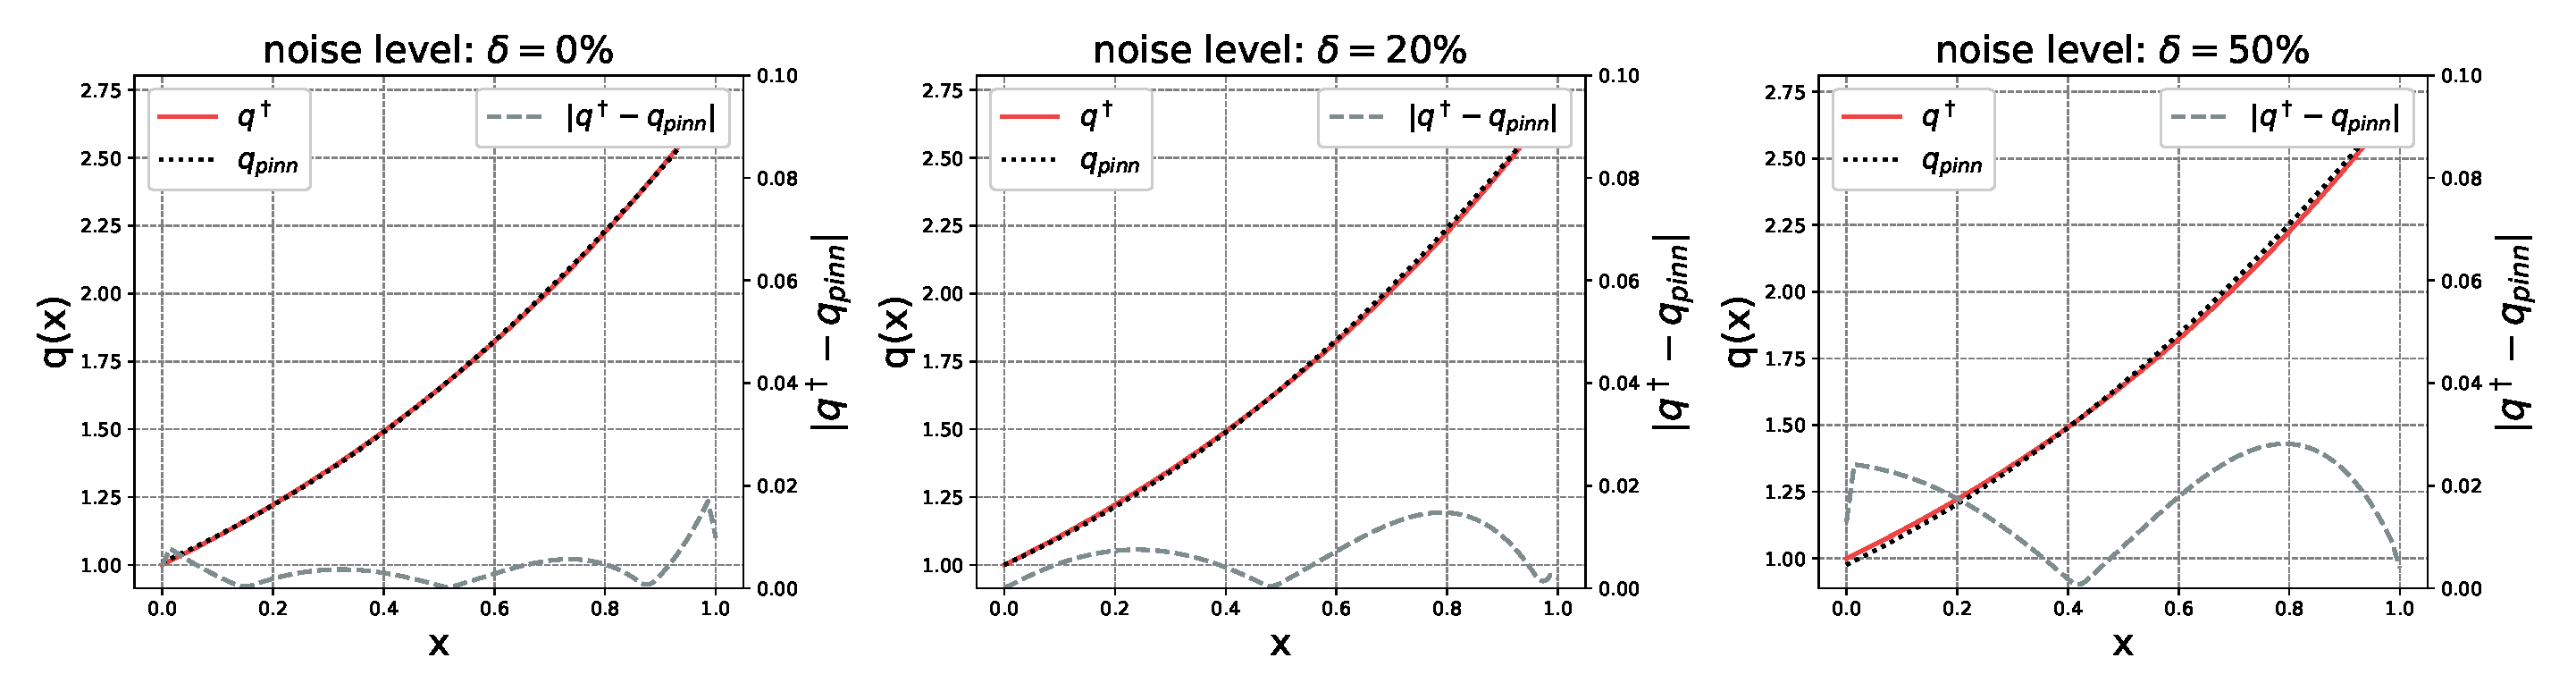
\includegraphics[width=\textwidth]{figures3/ex0_q.eps}
    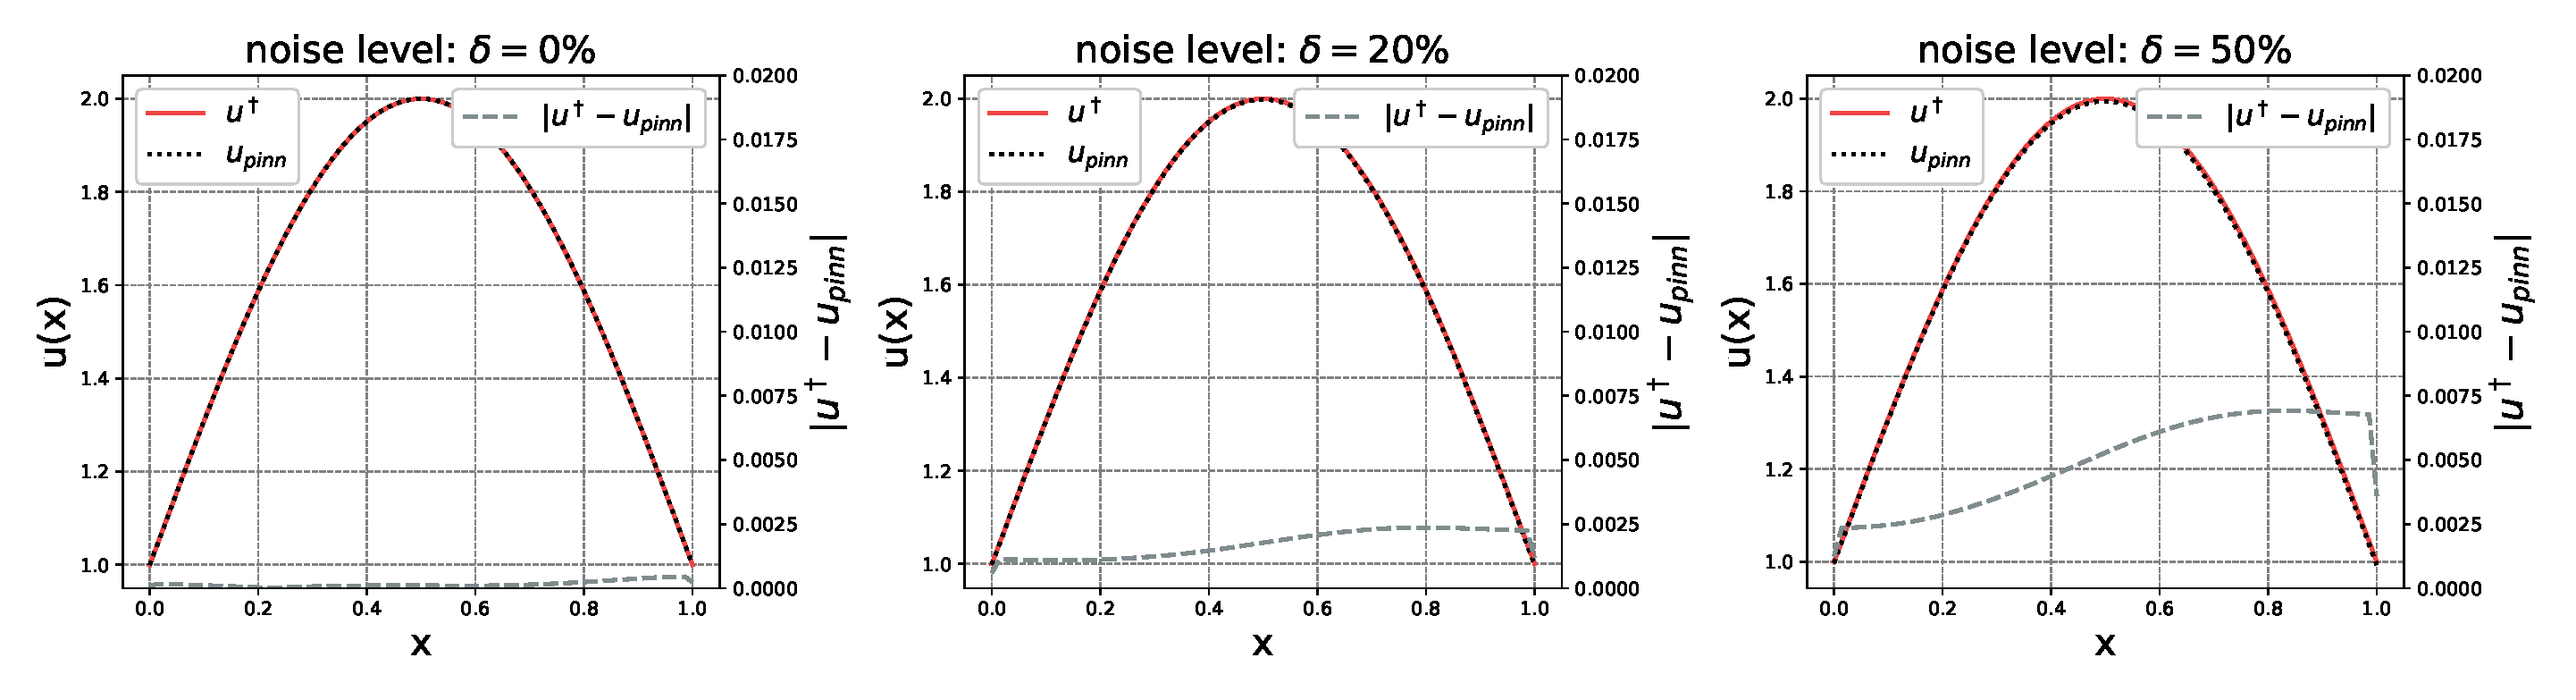
\includegraphics[width=\textwidth]{figures3/ex0_u.eps}
    \caption{例 \ref{example:1d} 的精确解、Tikhonov-PINN 解和绝对误差。第一行对应源项 $q$，第二行对应解 $u$。从左到右，结果是在不同的噪声水平下获得的。}
    \label{fig:ex0_q_u}
\end{figure}

在本小节中，我们使用一个一维例子来验证 Tikhonov-PINNs 的收敛率，并研究超参数对重构误差的影响。
\begin{example}\label{example:1d}
令 $\Omega=(0,1)$ 且 $\alpha\equiv 1$，定义精确势函数为 $q^{\dagger}(x)=\exp(x)$，对应的解为 $u^{\dagger}(x) = 1+\sin(\pi x)$。源项 $f$ 和边界条件 $g$ 由模型方程 Eq.\eqref{eq:pde:potential} 确定。
\end{example}

$q$ 和 $u$ 的精确解与 Tikhonov-PINNs 解如图 \ref{fig:ex0_q_u} 所示。在本例中，我们设置 $\lambda=10^{-7}$，采样 50,000 个内部点，并将边界点设为 \{0, 1\}。优化使用 Adam 优化器进行，学习率为 $10^{-4}$，迭代次数为 10,000 次。我们采用一个具有 $tanh$ 激活函数且宽度为 64 的两层神经网络来逼近 $q$ 和 $u$，并在架构中每两个相邻隐藏层之间应用残差连接。除非另有说明，本小节中的所有一维算例均使用与本例相同的默认参数设置。

\subsubsection{收敛率}
在定理 \ref{thm:ConvergenceRate} 中，我们建立了 $q$ 和 $u$ 关于噪声水平 $\delta$ 的收敛率。为了验证这一结果，我们计算了不同噪声水平下 $q$ 和 $u$ 的相对误差，结果如图 \ref{fig:ex0:noise} 所示。

\begin{figure}[htbp]
    \centering
    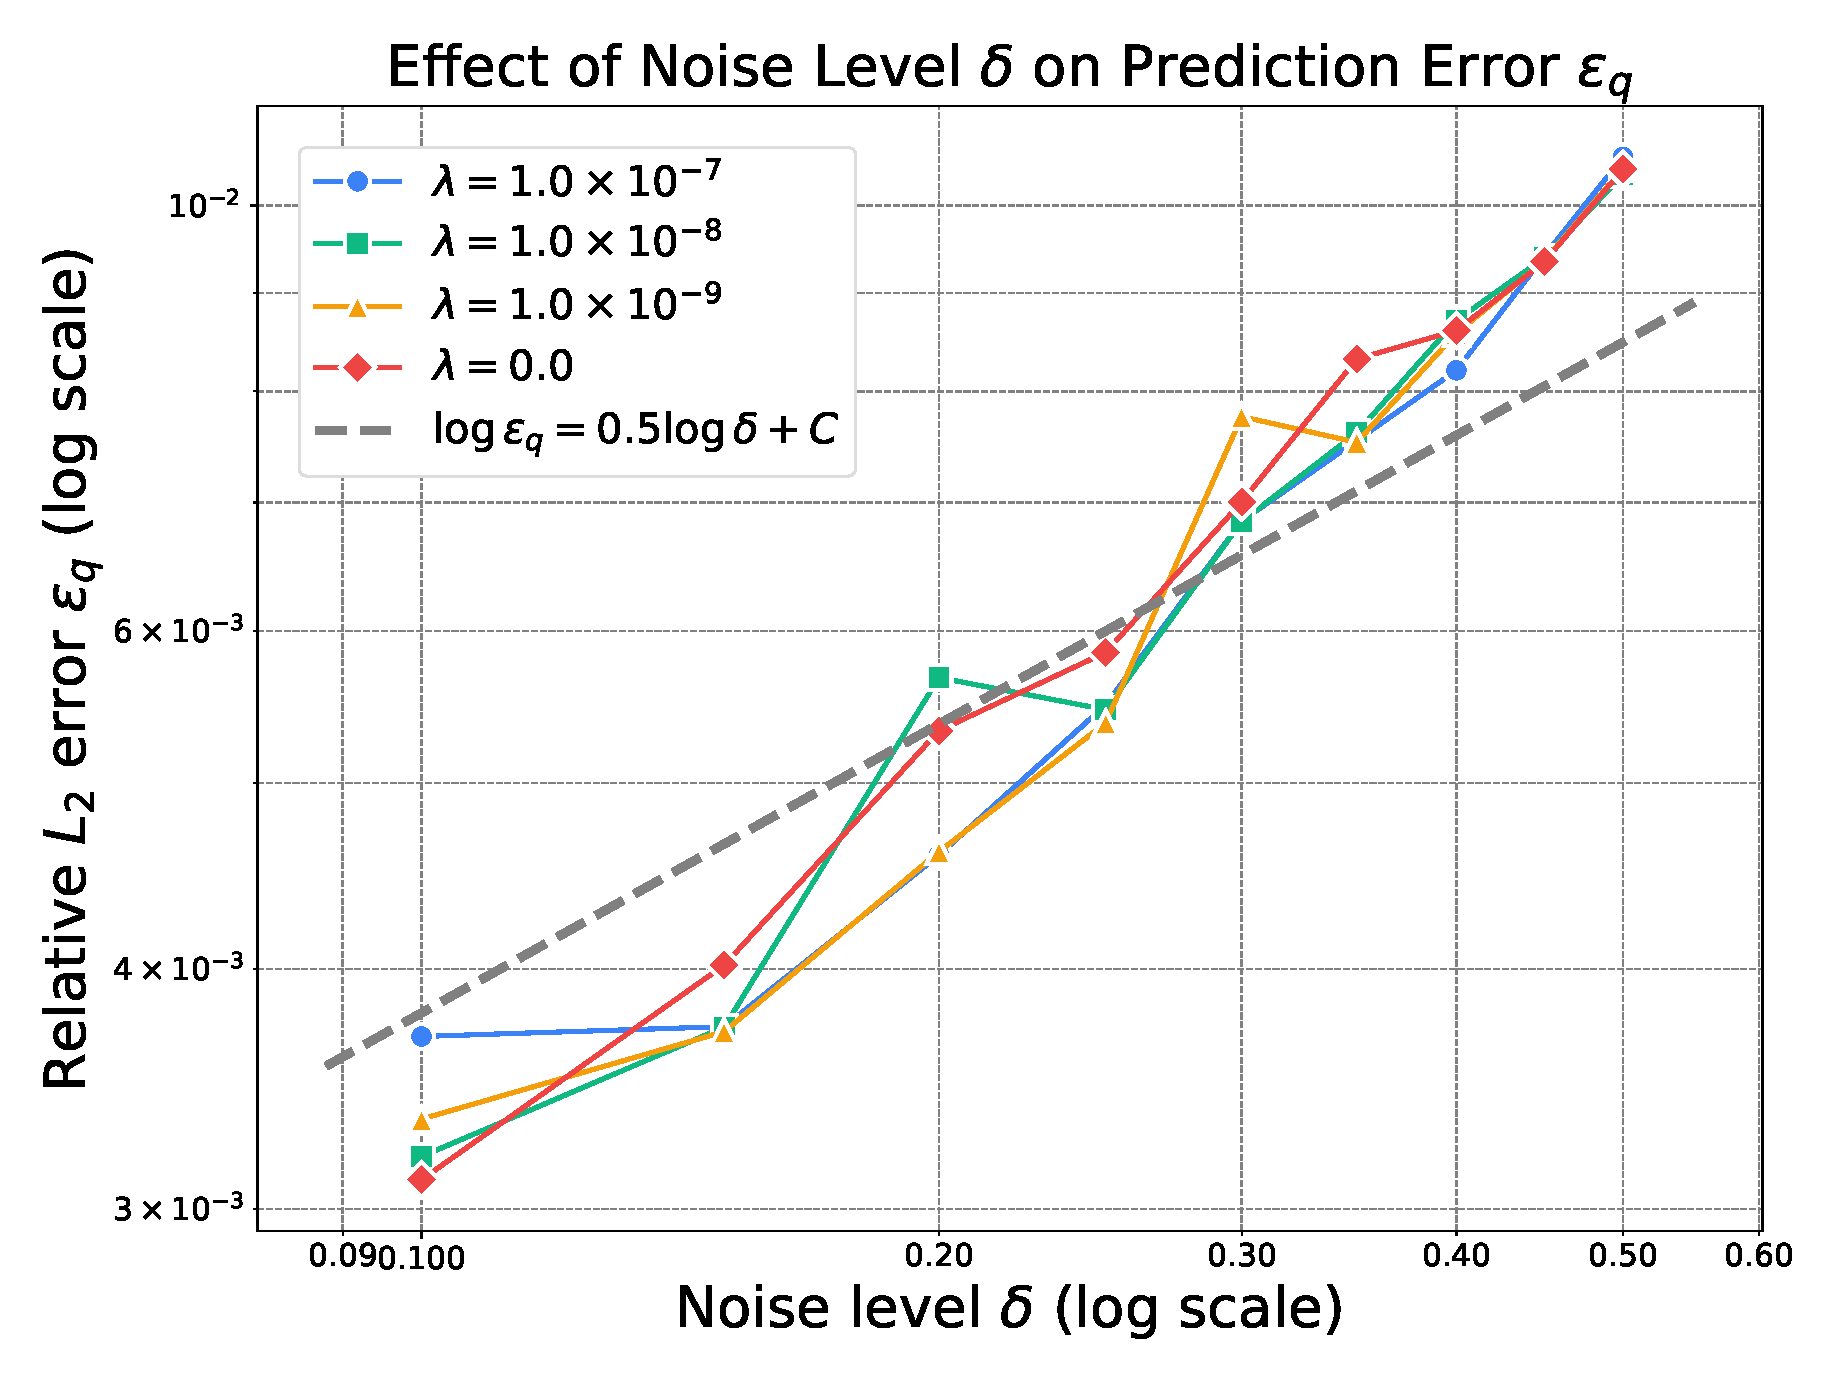
\includegraphics[width=0.49\textwidth]{figures3/ex0_noise_q.eps}
    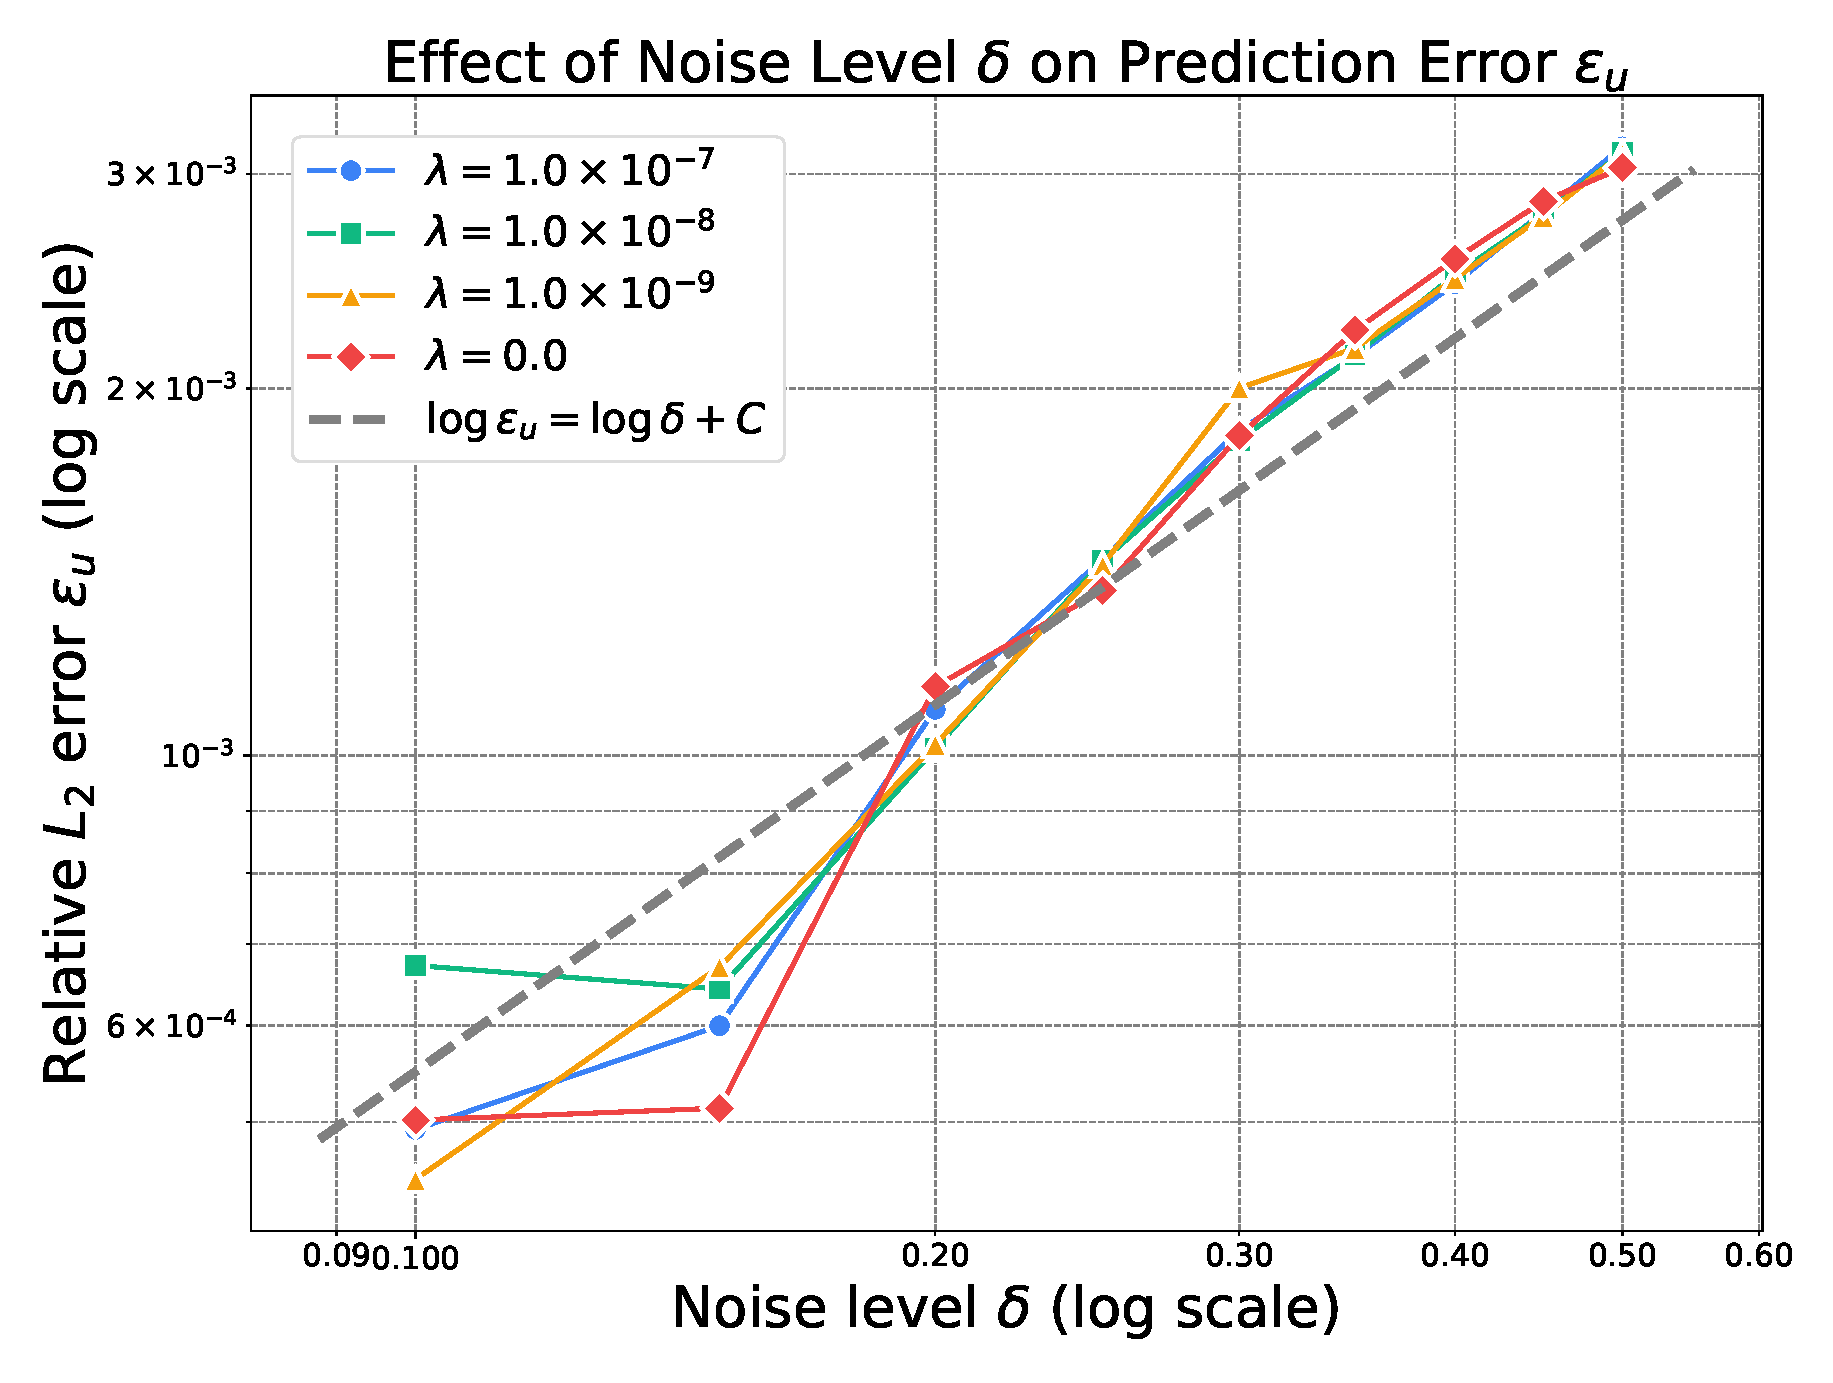
\includegraphics[width=0.49\textwidth]{figures3/ex0_noise_u.eps}
    \caption{不同正则化参数下噪声水平对解误差的影响。左图显示了 $q$ 的结果，其中 $\lambda=$$10^{-7}$, $10^{-8}$, $10^{-9}$ 和 0 对应的对数回归曲线的斜率分别为 0.708、0.748、0.760 和 0.743，平均斜率为 0.744。右图显示了 $u$ 的结果，其中对应的斜率分别为 1.22、1.08、1.25 和 1.26，平均斜率为 1.21。}
    \label{fig:ex0:noise}
\end{figure}

由于目标势函数具有正下界，该算例满足 $\beta = 0$ 的正性条件。根据定理~\ref{thm:ConvergenceRate} 和注 \ref{compare_Gar}，$q$ 和 $u$ 的收敛率可以任意接近 $O(\delta^{0.5})$ 和 $O(\delta)$。这一点在图 \ref{fig:ex0:noise} 中得到了检验，其中 $u$ 和 $q$ 的数值收敛率与理论收敛率非常一致。平均而言，在不同的 $\lambda$ 值下，我们观察到 $u$ 的经验收敛率为 $O(\delta^{1.21})$，$q$ 的经验收敛率为 $O(\delta^{0.74})$，这实际上快于理论收敛率，表明我们的理论界可能不是最优的。

\subsubsection{正则化的影响}
在本小节中，我们要研究不同正则化在求解算例 \ref{example:1d} 时的影响。如表 \ref{tab:regularization} 所示，当训练样本量相对较小（表 1 中的第一个子表）时，与 $L^2$ 正则化或原始 PINNs 相比，$H^2$ 正则化显著降低了 $q$ 的相对误差，尤其是当正则化系数 $\lambda$ 相对较大时。第二个子表表明，随着更多训练样本的可用，这种改进变得不那么明显。这是符合预期的，因为适当的正则化和增加数据量都有助于防止过拟合并提高精度。尽管如此，在两种情况下，当 $\lambda$ 选择得当时，$H^2$ 正则化都能产生最小的重构误差。这些结果凸显了 $H^2$ 正则化在求解此类反势问题时的有效性和优越性。

\begin{table}[hbtp]
\centering
\footnotesize
\caption{算例 \ref{example:1d} 中不同正则化下 $\hat{q}$ 的相对 $L^{2}$ 误差。}
\begin{tabular}{lrrrrr}
\hline
\multirow{2}[0]{*}{$\text{err}(q_{\text{pinn}})$} & \multicolumn{5}{c}{正则化参数 $\lambda$} \\
\cline{2-6}
& \multicolumn{1}{l}{$1.0\times 10^{-3}$} & 
\multicolumn{1}{l}{$1.0\times 10^{-4}$} &
\multicolumn{1}{l}{$1.0\times 10^{-5}$} &
\multicolumn{1}{l}{$1.0\times 10^{-6}$} & 
\multicolumn{1}{l}{$1.0\times 10^{-7}$} \\
   \hline
$H^2$ 正则化 & $5.44\times 10^{-2}$ & $\textbf{5.26}\times \textbf{10}^{-2}$ & $8.27\times 10^{-2}$ & $8.99\times 10^{-2}$ & $9.07\times 10^{-2}$ \\
$L^2$ 正则化 & $9.35\times 10^{-2}$ & $9.11\times 10^{-2}$ & $9.08\times 10^{-2}$ & $9.08\times 10^{-2}$ & $9.08\times 10^{-2}$ \\
无正则化 & $9.08\times 10^{-2}$ & $9.08\times 10^{-2}$ & $9.08\times 10^{-2}$ & $9.08\times 10^{-2}$ & $9.08\times 10^{-2}$  \\
\hline
&       &       &       &       & \\
\hline
\multirow{2}[0]{*}{$\text{err}(q_{\text{pinn}})$} & \multicolumn{5}{c}{正则化参数 $\lambda$} \\
\cline{2-6}
& \multicolumn{1}{l}{$1.0\times 10^{-3}$} & 
\multicolumn{1}{l}{$1.0\times 10^{-4}$} &
\multicolumn{1}{l}{$1.0\times 10^{-5}$} &
\multicolumn{1}{l}{$1.0\times 10^{-6}$} & 
\multicolumn{1}{l}{$1.0\times 10^{-7}$} \\
\hline
$H^2$ 正则化 & $8.96\times 10^{-2}$ & $3.14\times 10^{-2}$ & $\textbf{2.94}\times \textbf{10}^{-2}$ & $3.03\times 10^{-2}$ & $3.04\times 10^{-2}$  \\
$L^2$ 正则化 & $3.80\times 10^{-2}$ & $3.10\times 10^{-2}$ & $3.05\times 10^{-2}$ & $3.04\times 10^{-2}$ & $3.04\times 10^{-2}$ \\
无正则化 & $3.04\times 10^{-1}$ & $3.04\times 10^{-2}$ & $3.04\times 10^{-2}$ & $3.04\times 10^{-2}$ & $3.04\times 10^{-2}$ \\
\hline

\end{tabular}
\label{tab:regularization}
\end{table}

\subsubsection{其他超参数的影响}

\begin{figure}[htbp]
    \centering
    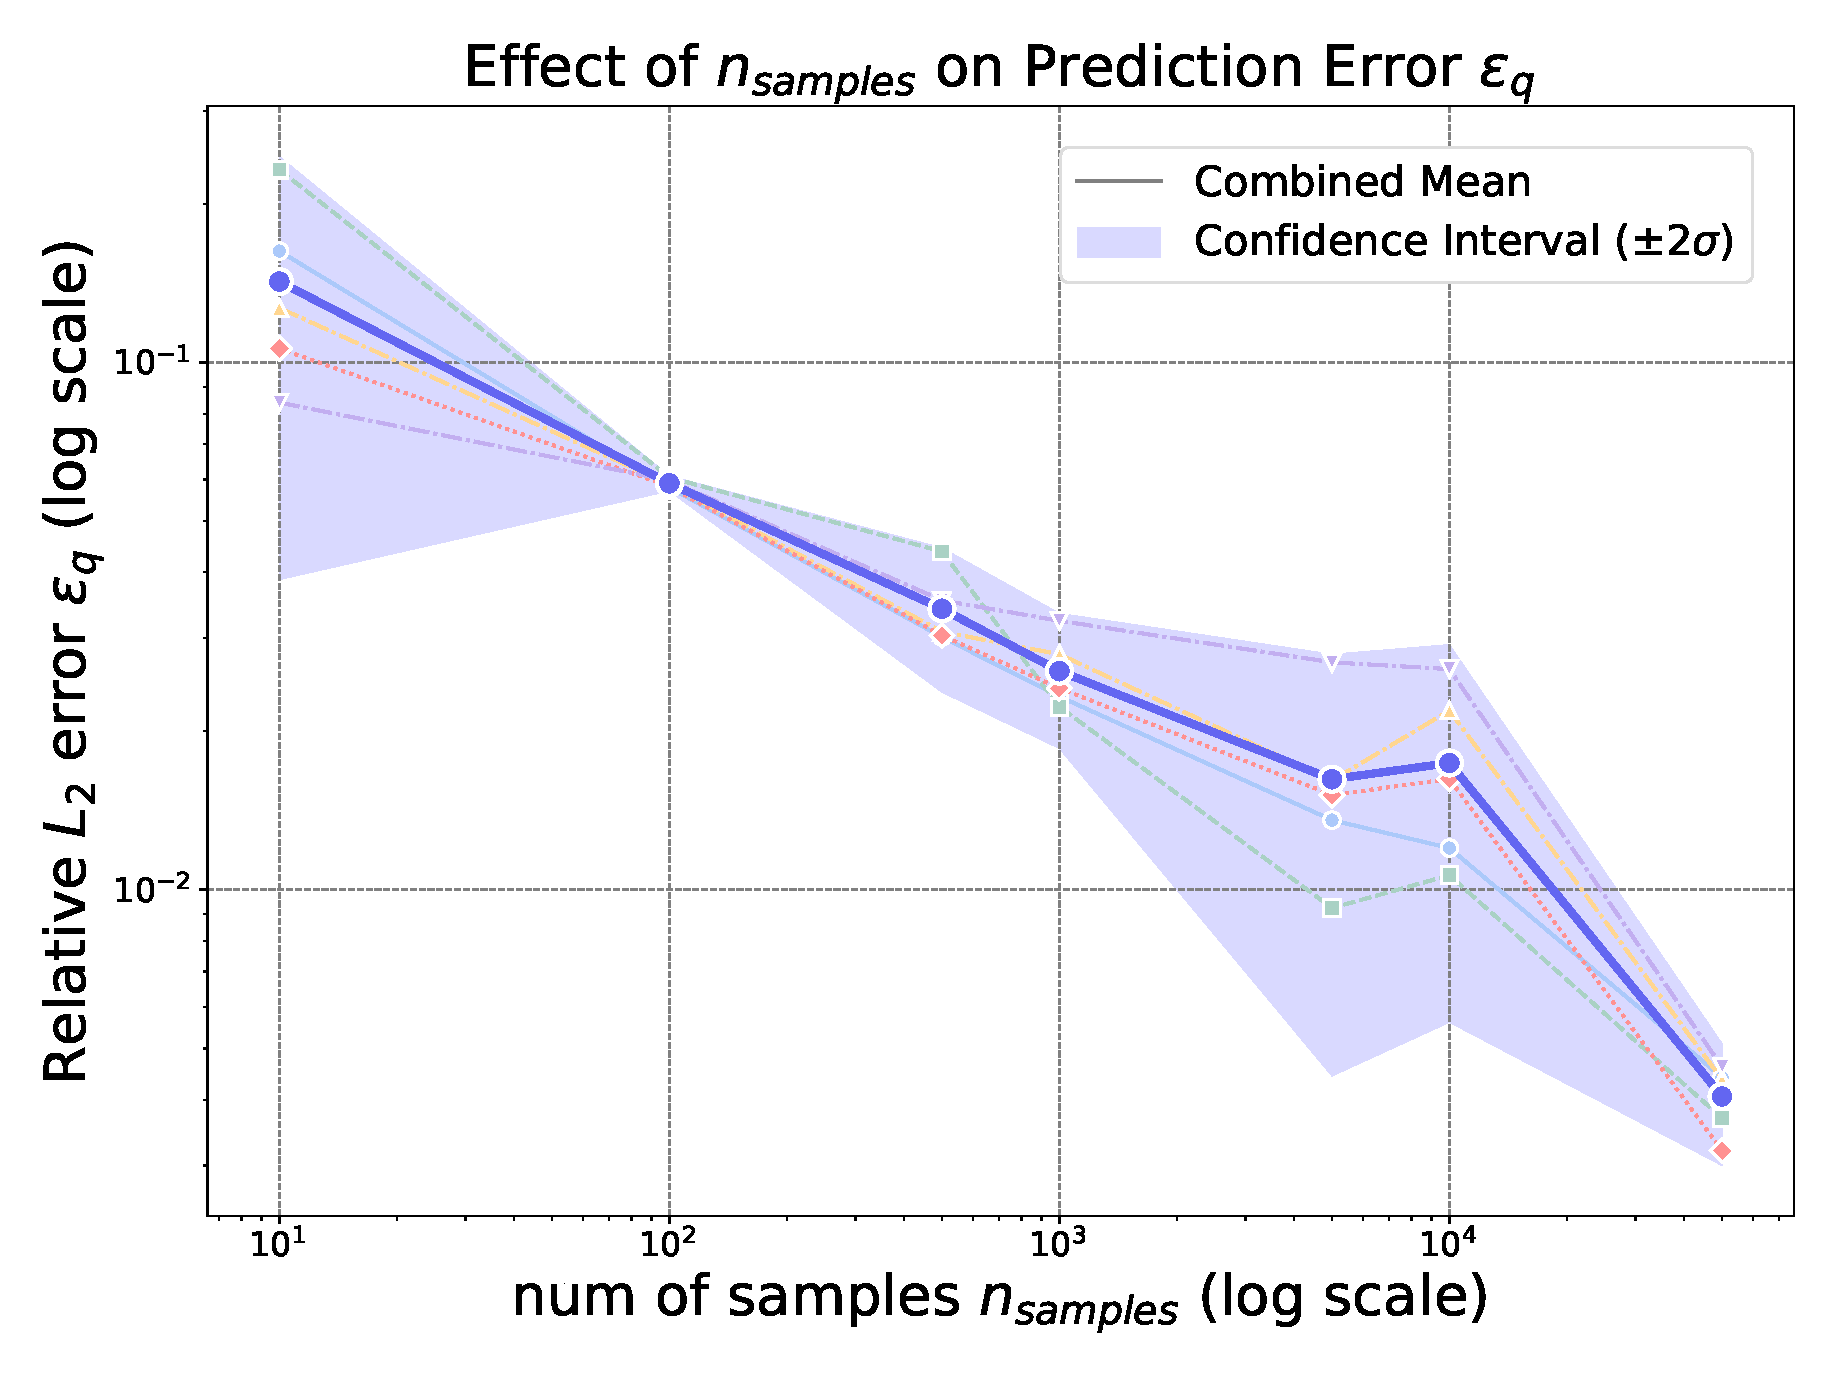
\includegraphics[width=0.48\textwidth]{figures3/ex0_nsample.eps}
    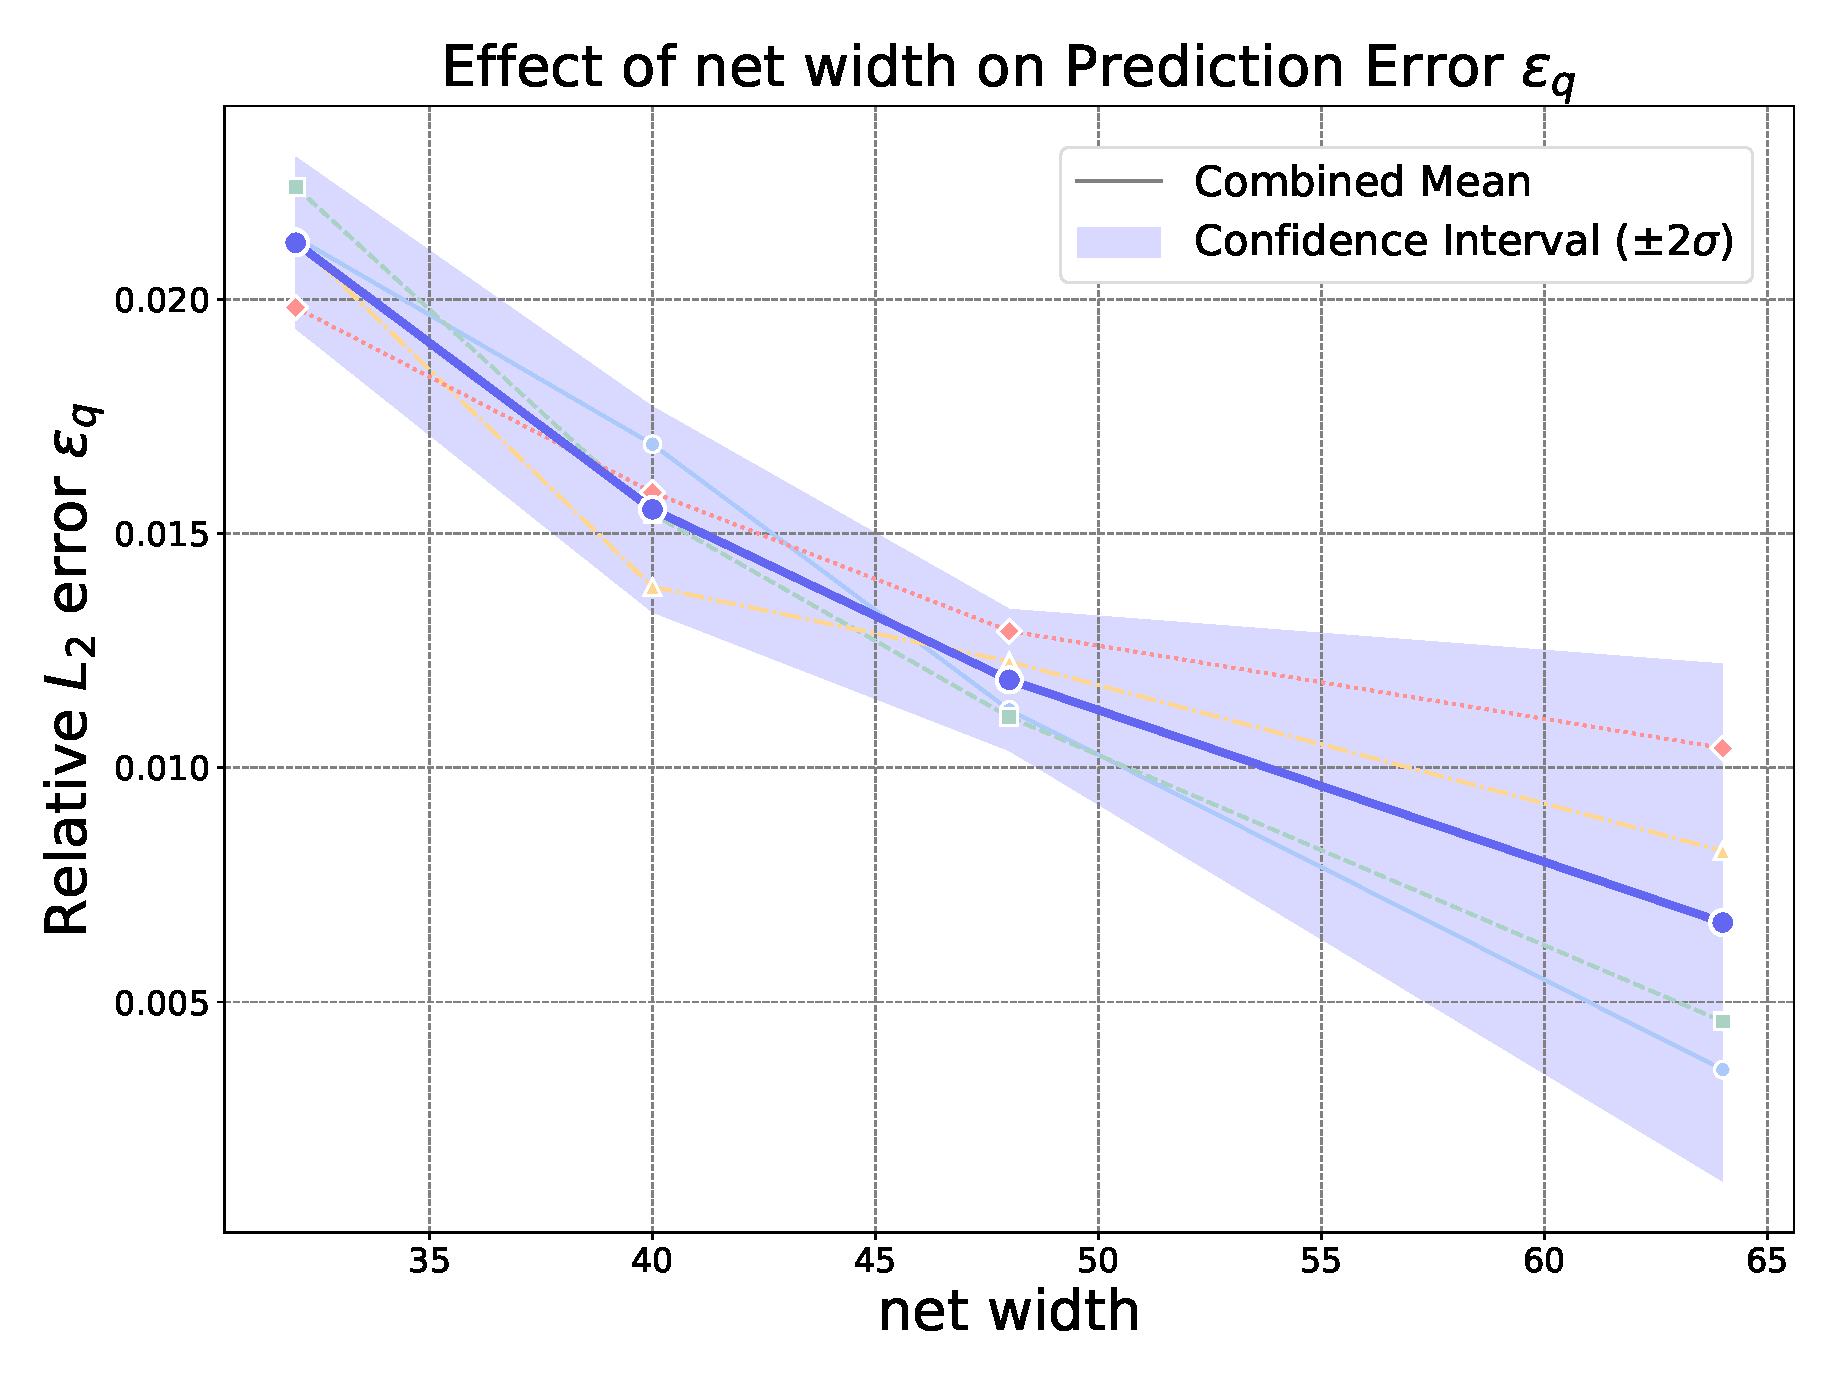
\includegraphics[width=0.48\textwidth]{figures3/ex0_width.eps}
    \caption{样本大小和网络宽度对算法精度的影响。我们进行了多次运行，并展示了相应的置信区间。特别地，由于网络深度是固定的，非零参数的数量 $R_{\calQ}$ 与网络宽度近似成正比。}
    \label{fig:ex0:width}
\end{figure}

我们研究了神经网络复杂度和样本复杂度对模型性能的影响。根据定理 \ref{thm:ConvergenceRate} 和假设 \ref{allcondition}，要实现更低的重构误差，需要增加样本大小和网络规模。我们通过以下实验验证了这种单调关系。在图~\ref{fig:ex0:width} 左侧，我们固定网络架构并改变样本大小以考察其影响。在图~\ref{fig:ex0:width} 右侧，我们保持两层的网络深度，同时调整网络宽度，从而按比例缩放神经元总数 $R_\mathbf{\calQ}$。对每个设置都进行了多次运行，图中显示的结果表明，误差随着样本大小和参数数量的增加而减小。

\subsubsection{二维问题}
接下来我们展示一个二维光滑算例，其中待反演的 $q^{\dagger}$ 和 $u^{\dagger}$ 均呈现正弦函数形式。

\begin{example}\label{example:onemode}
令 $\Omega=(0,1)^{2}$ 且 $\alpha\equiv 1$。我们考虑对以下势函数的识别
\begin{equation*}
q^{\dagger}(x_{1},x_{2})=1+0.5\times\sin(\pi x_{1})\sin(\pi x_{2}),
\end{equation*}
且精确解 $u^{\dagger}$ 为：
\[
u^{\dagger}(x_{1},x_{2})=1+\sin(\pi x_{1})\sin(\pi x_{2}).
\]
\end{example}

在本实验中，神经网络包含两个宽度为 64 的隐藏层。我们在内部和边界上共采样 100,000 个点，并使用学习率为 $10^{-4}$ 的 Adam 优化器训练模型 50,000 次迭代。

我们还使用有限元方法 (FEM) 求解了相同的问题。在 FEM 实现中，采用了一阶拉格朗日单元，并利用 L-BFGS 算法对解进行了 50 次迭代优化。为了确保比较的公平性，区域 $[0,1]^2$ 被离散化为 $320\times 320=102,400$ 个网格点，这与 Tikhonov-PINNs 中使用的总样本数（$100,000$ 个样本）相当。

\begin{figure}[htbp]
    \centering
    % 第一个子图：Tikhonov-PINNs 方法（假设文件名暗示这是神经网络方法）
    \begin{subfigure}[b]{\textwidth}
        \centering
        % 插入图片
        \includegraphics[width=\textwidth]{figures3/one_peak_nn.eps}
        % 简短的子标题
        \caption{Tikhonov-PINNs 方法结果}
        \label{fig:one_peak_nn}
    \end{subfigure}
    \hfill % 填充中间空白，让图片分别对齐左右
    % 第二个子图：有限元方法 (FEM)
    \begin{subfigure}[b]{\textwidth}
        \centering
        % 插入图片
        \includegraphics[width=\textwidth]{figures3/one_peak_fem.eps}
        % 简短的子标题
        \caption{有限元方法 (FEM) 结果}
        \label{fig:one_peak_fem}
    \end{subfigure}
    
    % 总标题：包含详细描述
    \caption{两种方法重构结果的比较：(a) Tikhonov-PINNs 和 (b) 有限元方法 (FEM)。
    左侧小图展示了例 \ref{example:onemode} 中势函数 $q^{\dagger}$（上）和解 $u^{\dagger}$（下）的真值；
    右侧小图展示了在不同噪声水平 $\delta$ 下，使用最优正则化参数 $\lambda$ 重构的势 $\hat{q}$ 和解 $\hat{u}$。}
    \label{fig:example:one_peak}
\end{figure}


数值结果如图~\ref{fig:example:one_peak} 所示。这里，基于各种实验，$\lambda$ 被选为最优正则化参数。为了进一步阐明噪声 $\delta$ 的影响，我们在表~\ref{tab:onemode} 中提供了不同正则化参数 $\lambda$ 下相对误差的详细比较。显然，在低噪声水平下，FEM 和 Tikhonov-PINNs 方法均能有效地重构 $q$ 和 $u$。此外，随着噪声水平的增加，$q$ 的误差逐渐增大，这与我们的理论发现相符。在大多数情况下，FEM 优于 Tikhonov-PINNs 方法，当 $\lambda$ 选择得当时，产生的相对 $L^2$ 误差更低。这突显了 FEM 在处理此类光滑问题时的优越性，特别是在低维情况下。然而，正如第~\ref{sec:semi_converge} 节所讨论的，FEM 中的半收敛现象需要仔细的早停策略。此外，对于非光滑和高维问题，Tikhonov-PINNs 表现出优于标准 FEM 的性能。我们将在后续章节中对此进行讨论。

聚焦于 Tikhonov-PINNs 的结果，很明显，较高的噪声水平需要较大的正则化参数 $\lambda$，以在重构解中获得最佳的误差控制。噪声强度与正则化参数之间的这种单调关系与定理~\ref{thm:ConvergenceRate} 中的分析一致。

\begin{table}[htbp]
   \centering
   \footnotesize
   \caption{例 \ref{example:onemode} 中重构势 $\hat{q}$ 和解 $\hat{u}$ 的相对 $L^{2}$ 误差。}
   \begin{tabular}{lllllll}
   \hline
   \multirow{2}[0]{*}{$\delta  = 1\%$} & \multicolumn{6}{c}{正则化参数 $\lambda$} \\
   \cline{2-7}
   & $1.0\times 10^{-5}$ & $1.0\times 10^{-6}$ & $1.0\times 10^{-7}$ & $1.0\times 10^{-8}$ & $1.0\times 10^{-9}$ & \multicolumn{1}{r}{0} \\
   \hline
   $\text{err}(u_{\text{pinn}})$ & $3.14\times 10^{-3}$ & $1.49\times 10^{-3}$ & $7.67\times 10^{-4}$ & $5.99\times 10^{-4}$ & $5.81\times 10^{-4}$ & $5.72\times 10^{-4}$ \\
   $\text{err}(u_{\text{fem}})$ & $1.93\times 10^{-4}$ & $1.84\times 10^{-4}$ & $1.19\times 10^{-4}$ & $1.44\times 10^{-4}$ & $1.68\times 10^{-4}$ & $1.03\times 10^{-4}$ \\
   $\text{err}(q_{\text{pinn}})$ & $1.46\times 10^{-1}$ & $5.39\times 10^{-2}$ & $3.39\times 10^{-2}$ & $3.27\times 10^{-2}$ & $3.27\times 10^{-2}$ & $3.27\times 10^{-2}$ \\
   $\text{err}(q_{\text{fem}})$ & $1.44\times 10^{-2}$ & \textbf{1.23$\times $10$^{-2}$} & $6.26\times 10^{-3}$ & $1.27\times 10^{-2}$ & $1.68\times 10^{-2}$ & $1.95\times 10^{-2}$ \\
   \hline
   &       &       &       &       &       &  \\
   \hline
   \multirow{2}[0]{*}{$\delta = 10\%$} & \multicolumn{6}{c}{正则化参数 $\lambda$} \\
   \cline{2-7}
   & $1.0\times 10^{-5}$ & $1.0\times 10^{-6}$ & $1.0\times 10^{-7}$ & $1.0\times 10^{-8}$ & $1.0\times 10^{-9}$ & \multicolumn{1}{r}{0} \\
   \hline
   $\text{err}(u_{\text{pinn}})$ & $3.08\times 10^{-3}$ & $1.97\times 10^{-3}$ & $1.48\times 10^{-3}$ & $1.41\times 10^{-3}$ & $1.40\times 10^{-3}$ & $1.40\times 10^{-3}$ \\
   $\text{err}(u_{\text{fem}})$ & $1.09\times 10^{-3}$ & $6.30\times 10^{-4}$ & $1.71\times 10^{-3}$ & $2.51\times 10^{-3}$ & $2.71\times 10^{-3}$ & $3.43\times 10^{-3}$\\
   $\text{err}(q_{\text{pinn}})$ & $1.50\times 10^{-1}$ & $6.18\times 10^{-2}$ & $4.33\times 10^{-2}$ & $4.13\times 10^{-2}$ & $4.11\times 10^{-2}$ & $4.11\times 10^{-2}$ \\
   $\text{err}(q_{\text{fem}})$ & \textbf{1.72$\times $10$^{-2}$} & $2.84\times 10^{-2}$ & $8.56\times 10^{-2}$ & $3.23\times 10^{-1}$ & $3.80\times 10^{-1}$ & $5.40\times 10^{-1}$\\
   \hline
   &       &       &       &       &       &  \\
   \hline
   \multirow{2}[0]{*}{$\delta = 20\%$} & \multicolumn{6}{c}{正则化参数 $\lambda$} \\
   \cline{2-7}
   & $1.0\times 10^{-5}$ & $1.0\times 10^{-6}$ & $1.0\times 10^{-7}$ & $1.0\times 10^{-8}$ & $1.0\times 10^{-9}$ & \multicolumn{1}{r}{0} \\
   \hline
   $\text{err}(u_{\text{pinn}})$ & $3.38\times 10^{-3}$ & $2.47\times 10^{-3}$ & $2.19\times 10^{-3}$ & $2.17\times 10^{-3}$ & $2.17\times 10^{-3}$ & $2.17\times 10^{-3}$ \\
   $\text{err}(u_{\text{fem}})$ & $8.88\times 10^{-4}$ & $2.16\times 10^{-3}$ & $4.76\times 10^{-3}$ & $4.30\times 10^{-3}$ & $3.44\times 10^{-3}$ & $4.98\times 10^{-3}$ \\
   $\text{err}(q_{\text{pinn}})$ & $1.54\times 10^{-1}$ & $7.29\times 10^{-2}$ & $6.34\times 10^{-2}$ & $6.44\times 10^{-2}$ & $6.46\times 10^{-2}$ & $6.46\times 10^{-2}$ \\
   $\text{err}(q_{\text{fem}})$ & \textbf{1.89$\times $10$^{-2}$} & $8.56\times 10^{-2}$ & $2.64\times 10^{-1}$ & $3.85\times 10^{-1}$ & $4.35\times 10^{-1}$ & $4.98\times 10^{-1}$\\
   \hline
   &       &       &       &       &       &  \\
   \hline
   \multirow{2}[0]{*}{$\delta = 50\%$} & \multicolumn{6}{c}{正则化参数 $\lambda$} \\
   \cline{2-7}
   & $1.0\times 10^{-5}$ & $1.0\times 10^{-6}$ & $1.0\times 10^{-7}$ & $1.0\times 10^{-8}$ & $1.0\times 10^{-9}$ & \multicolumn{1}{r}{0} \\
   \hline
   $\text{err}(u_{\text{pinn}})$ & $4.14\times 10^{-3}$ & $5.22\times 10^{-3}$ & $5.20\times 10^{-3}$ & $5.22\times 10^{-3}$ & $5.22\times 10^{-3}$ & $5.22\times 10^{-3}$ \\
   $\text{err}(u_{\text{fem}})$ & $4.90\times 10^{-3}$ & $7.22\times 10^{-3}$ & $8.26\times 10^{-3}$ & $1.01\times 10^{-2}$ & $1.40\times 10^{-2}$ & $9.21\times 10^{-3}$ \\
   $\text{err}(q_{\text{pinn}})$ & $1.65\times 10^{-1}$ & $1.03\times 10^{-1}$ & $1.05\times 10^{-1}$ & $1.06\times 10^{-1}$ & $1.06\times 10^{-1}$ & $1.06\times 10^{-1}$ \\
   $\text{err}(q_{\text{fem}})$ & \textbf{5.64$\times $10$^{-2}$} & $2.32\times 10^{-1}$ & $5.85\times 10^{-1}$ & $0.85\times 10^{-1}$ & $1.10$ & $0.81\times 10^{-1}$\\
   \hline
   \end{tabular}
   \label{tab:onemode}%
\end{table}%

% \subsection{非光滑势问题}
% 为了进一步探索我们算法的局限性并评估神经网络对非光滑势的逼近能力，我们将我们的方法应用于几个非光滑算例，在这些算例中，诸如标准有限元方法 (FEM) 等传统方法的效果可能较差。参数设置保持与算例~\ref{example:onemode} 中相同。此外，我们将 Tikhonov-PINNs 方法的性能与经典有限元方法进行了比较。本节的 FEM 设置与算例 5.2 中的设置相同。

% \subsubsection{连续问题}
% 接下来，我们考虑如下定义的非光滑势函数的识别问题。

% \begin{example}\label{example:nonsmooth}
% % Table generated by Excel2LaTeX from sheet '5'
% 令 $\Omega=(0,1)^{2}$ 且 $\alpha\equiv 1$。定义精确势函数 $q^{\dagger}$ 为：
% \begin{align*}
% \zeta(x_{1},x_{2})&=\exp\{-25\times(x_{1}-0.6)^{2}-25\times(x_{2}-0.4)^{2}\}, \\
% q^{\dagger}(x_{1},x_{2})&=0.75+\min\{0.75,\max\{0.25,2\zeta(x_{1},x_{2})\}\},
% \end{align*}
% 精确解 $u^{\dagger}$ 为 $u^{\dagger}(x_{1},x_{2})=1+\sin(\pi x_{1})\sin(\pi x_{2})$。
% \end{example}
% 表 \ref{tab:nonsmooth} 展示了在不同 $\lambda$ 和 $\delta$ 下 $u$ 和 $q$ 的相对误差，并用粗体高亮了每种噪声水平下的最佳结果。正如我们所见，Tikhonov-PINNs 在所有配置下始终实现了约为 $\calO(10^{-2})$ 的 $q$ 相对误差，比有限元方法高出一个数量级。


% \begin{table}[htbp]
%    \centering
%    \footnotesize
%    \caption{Example \ref{example:nonsmooth} 中恢复的势 $\hat{q}$ 和解 $\hat{u}$ 的相对 $L^{2}$ 误差。}
%    \begin{tabular}{lllllll}
%    \hline
%    \multirow{2}[0]{*}{$\delta  = 1\%$} & \multicolumn{6}{c}{正则化参数 $\lambda$} \\
%    \cline{2-7}
%    & $1.0\times 10^{-5}$ & $1.0\times 10^{-6}$ & $1.0\times 10^{-7}$ & $1.0\times 10^{-8}$ & $1.0\times 10^{-9}$ & \multicolumn{1}{r}{0} \\
%    \hline
%    $\text{err}(u_{\text{pinn}})$ & $3.14\times 10^{-3}$ & $2.01\times 10^{-3}$ & $6.03\times 10^{-4}$ & $5.71\times 10^{-4}$ & $4.94\times 10^{-4}$ & $4.03\times 10^{-4}$ \\
%    $\text{err}(u_{\text{fem}})$& $2.60\times 10^{-3}$& $1.14\times 10^{-3}$& $7.09\times 10^{-4}$& $6.96\times 10^{-4}$ & $5.33\times 10^{-4}$ &$6.41\times 10^{-4}$\\
%    $\text{err}(q_{\text{pinn}})$ & $1.46\times 10^{-1}$& $9.63\times 10^{-2}$ & $1.82\times 10^{-2}$ & $1.60\times 10^{-2}$ & \textbf{1.57$\times$ 10$^{-2}$} & \textbf{1.57$\times$ 10$^{-2}$}   \\
%    $\text{err}(q_{\text{fem}})$& $1.28\times 10^{-1}$& $8.77\times 10^{-2}$& $7.39\times 10^{-2}$& $7.36\times 10^{-2}$ & $6.43\times 10^{-2}$ &$6.97\times 10^{-2}$\\
%    \hline
%    &       &       &       &       &       &  \\
%    \hline
%    \multirow{2}[0]{*}{$\delta = 10\%$} & \multicolumn{6}{c}{正则化参数 $\lambda$} \\
%    \cline{2-7}
%    & $1.0\times 10^{-5}$ & $1.0\times 10^{-6}$ & $1.0\times 10^{-7}$ & $1.0\times 10^{-8}$ & $1.0\times 10^{-9}$ & \multicolumn{1}{r}{0} \\
%    \hline
%    $\text{err}(u_{\text{pinn}})$ & $3.08\times 10^{-3}$ & $2.22\times 10^{-3}$ & $1.36\times 10^{-3}$ & $1.30\times 10^{-3}$ & $1.30\times 10^{-3}$ & $1.30\times 10^{-3}$ \\
%    $\text{err}(u_{\text{fem}})$& $2.82\times 10^{-3}$& $1.30\times 10^{-3}$& $1.44\times 10^{-3}$& $1.18\times 10^{-3}$ & $1.30\times 10^{-3}$&$2.36\times 10^{-3}$\\
%    $\text{err}(q_{\text{pinn}})$ & $1.50\times 10^{-1}$ & $1.03\times 10^{-1}$ & $1.78\times 10^{-2}$ & $1.60\times 10^{-2}$ & $1.71\times 10^{-2}$ & \textbf{1.58$\times$ 10$^{-2}$ }\\
%    $\text{err}(q_{\text{fem}})$& $1.29\times 10^{-1}$& $8.77\times 10^{-2}$& $7.95\times 10^{-2}$& $9.02\times 10^{-2}$ & $1.16\times 10^{-1}$&$1.90\times 10^{-1}$\\
%    \hline
%    &       &       &       &       &       &  \\
%    \hline
%    \multirow{2}[0]{*}{$\delta = 20\%$} & \multicolumn{6}{c}{正则化参数 $\lambda$} \\
%    \cline{2-7}
%    & $1.0\times 10^{-5}$ & $1.0\times 10^{-6}$ & $1.0\times 10^{-7}$ & $1.0\times 10^{-8}$ & $1.0\times 10^{-9}$ & \multicolumn{1}{r}{0} \\
%    \hline
%    $\text{err}(u_{\text{pinn}})$ & $3.38\times 10^{-3}$ & $2.30\times 10^{-3}$ & $1.44\times 10^{-3}$ & $1.35\times 10^{-3}$ & $1.36\times 10^{-3}$ & $1.36\times 10^{-3}$ \\
%    $\text{err}(u_{\text{fem}})$& $2.67\times 10^{-3}$& $2.17\times 10^{-3}$& $4.23\times 10^{-3}$&$ 3.75\times 10^{-3}$ & $2.50\times 10^{-3}$&$4.15\times 10^{-3}$\\
%    $\text{err}(q_{\text{pinn}})$ & $1.54\times 10^{-1}$ & $9.09\times 10^{-2}$ & $1.71\times 10^{-2}$ & $1.60\times 10^{-2}$ & \textbf{1.59$\times$ 10$^{-2}$} & \textbf{1.59$\times$ 10$^{-2}$} \\
%    $\text{err}(q_{\text{fem}})$& $1.27\times 10^{-1}$& $9.77\times 10^{-2}$& $2.21\times 10^{-1}$& $2.13\times 10^{-1}$ & $1.51\times 10^{-1}$&$3.79\times 10^{-1}$\\
%    \hline
%    &       &       &       &       &       &  \\
%    \hline
%    \multirow{2}[0]{*}{$\delta = 50\%$} & \multicolumn{6}{c}{正则化参数 $\lambda$} \\
%    \cline{2-7}
%    & $1.0\times 10^{-5}$ & $1.0\times 10^{-6}$ & $1.0\times 10^{-7}$ & $1.0\times 10^{-8}$ & $1.0\times 10^{-9}$ & \multicolumn{1}{r}{0} \\
%    \hline
%    $\text{err}(u_{\text{pinn}})$ & $4.14\times 10^{-3}$ & $4.43\times 10^{-3}$ & $4.07\times 10^{-3}$ & $3.43\times 10^{-3}$ & $4.01\times 10^{-3}$ & $4.04\times 10^{-3}$ \\
%    $\text{err}(u_{\text{fem}})$& $4.41\times 10^{-3}$& $7.14\times 10^{-3}$& $7.90\times 10^{-3}$& $7.64\times 10^{-3}$& $1.26\times 10^{-2}$&$8.40\times 10^{-3}$\\
%    $\text{err}(q_{\text{pinn}})$ & $1.65\times 10^{-1}$ & $1.22\times 10^{-1}$ & $6.30\times 10^{-2}$ & \textbf{3.16}$\times$ \textbf{10}$^{-2}$ & $4.99\times 10^{-2}$ & $5.14\times 10^{-1}$ \\
%    $\text{err}(q_{\text{fem}})$& $1.45\times 10^{-1}$& $2.14\times 10^{-1}$& $4.64\times 10^{-1}$& $4.09\times 10^{-1}$& $9.07\times 10^{-1}$&$5.90\times 10^{-1}$\\
%    \hline
%    \end{tabular}%
%    \label{tab:nonsmooth}%
% \end{table}%

% \begin{figure}[htbp]
% \centering
% \setlength{\abovecaptionskip}{10pt}
% 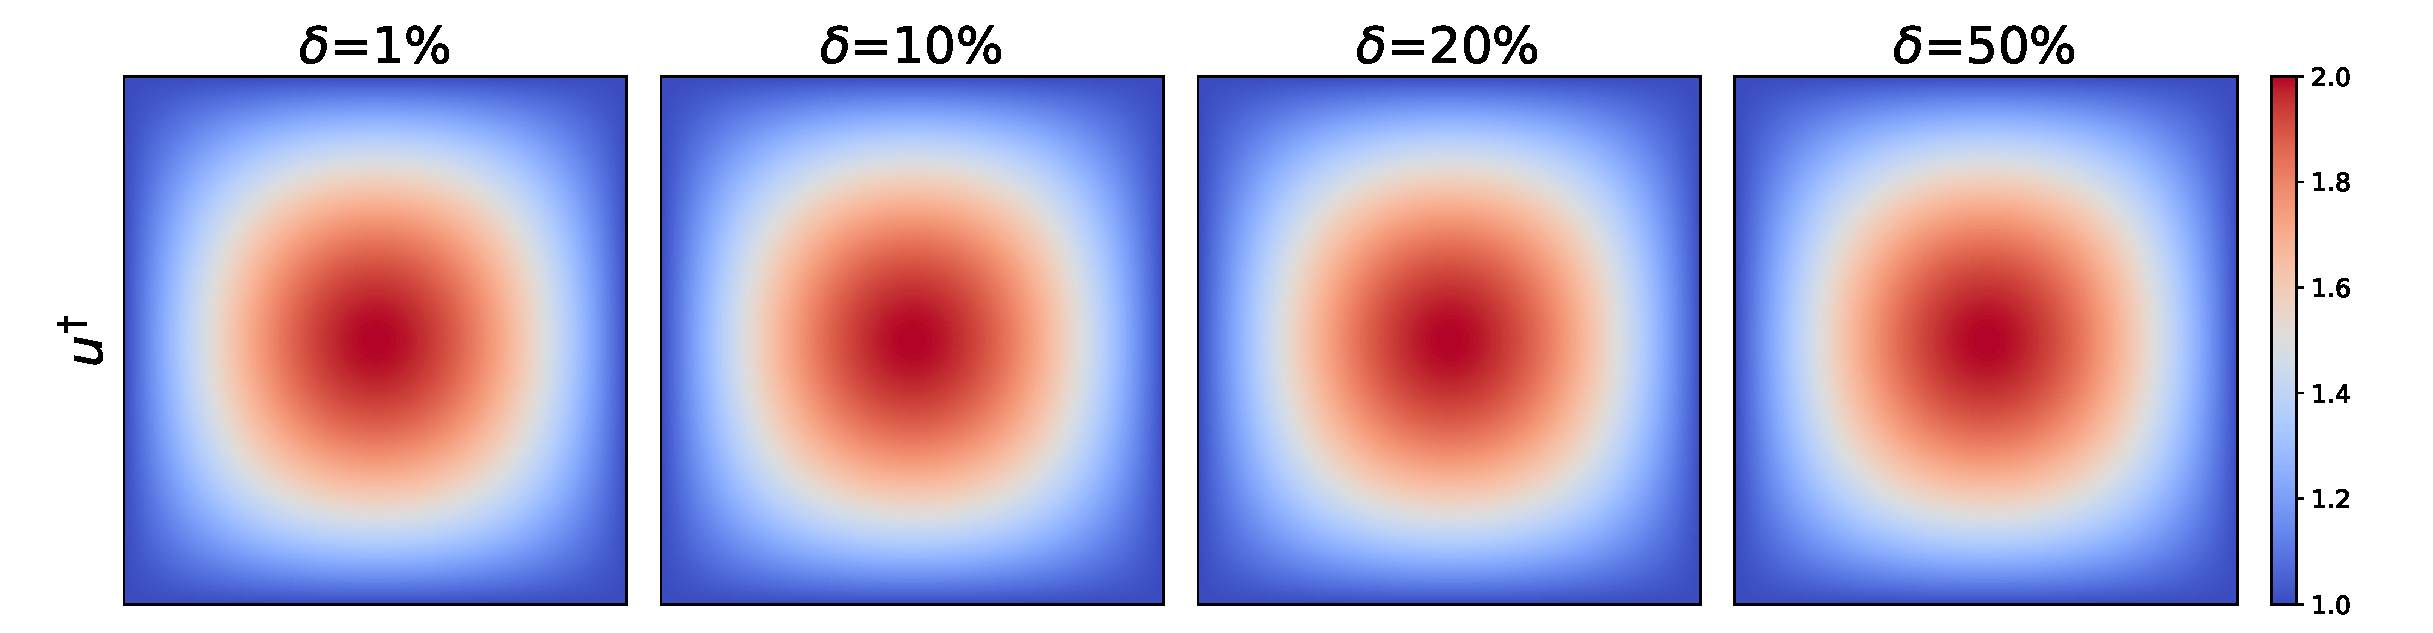
\includegraphics[width=\textwidth]{figures3/non_smooth_udag.eps}\par
% 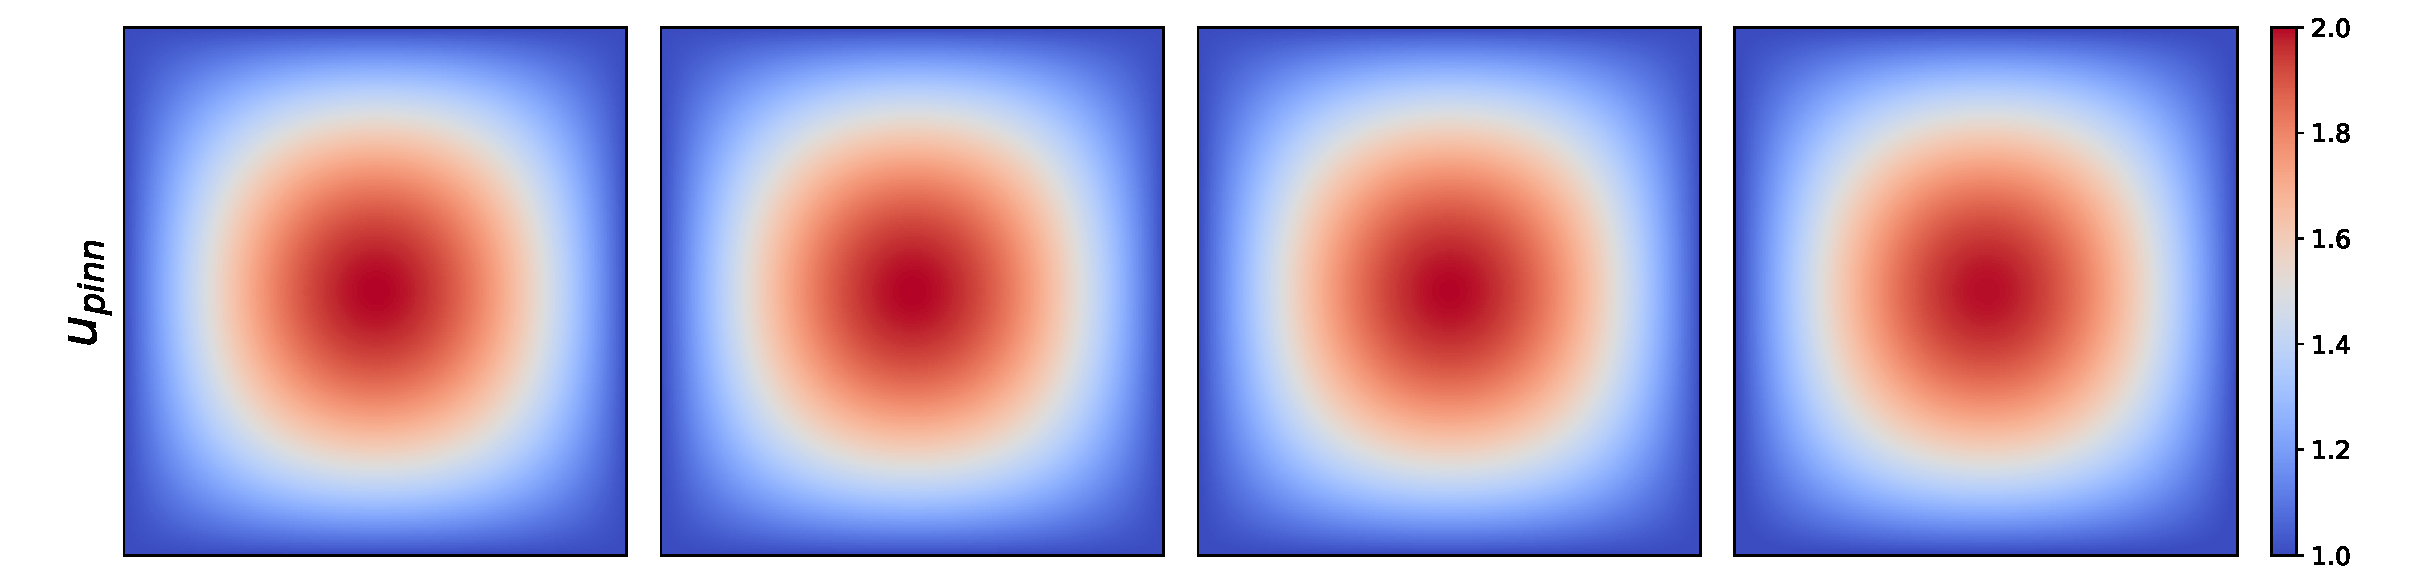
\includegraphics[width=\textwidth]{figures3/non_smooth_unn.eps}\par
% 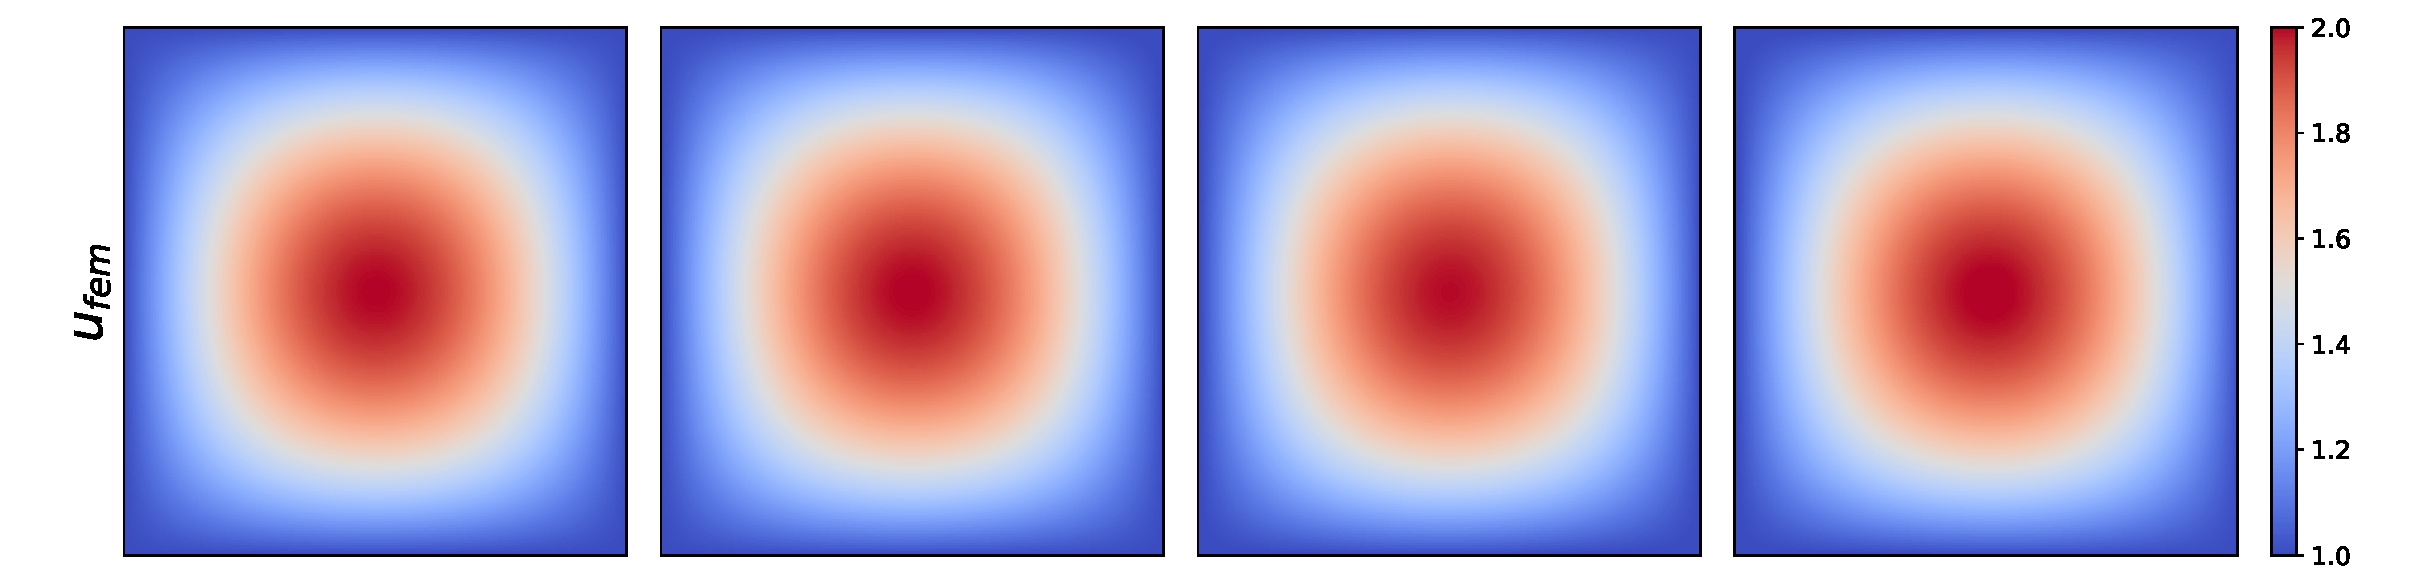
\includegraphics[width=\textwidth]{figures3/non_smooth_ufem.eps}\par
% 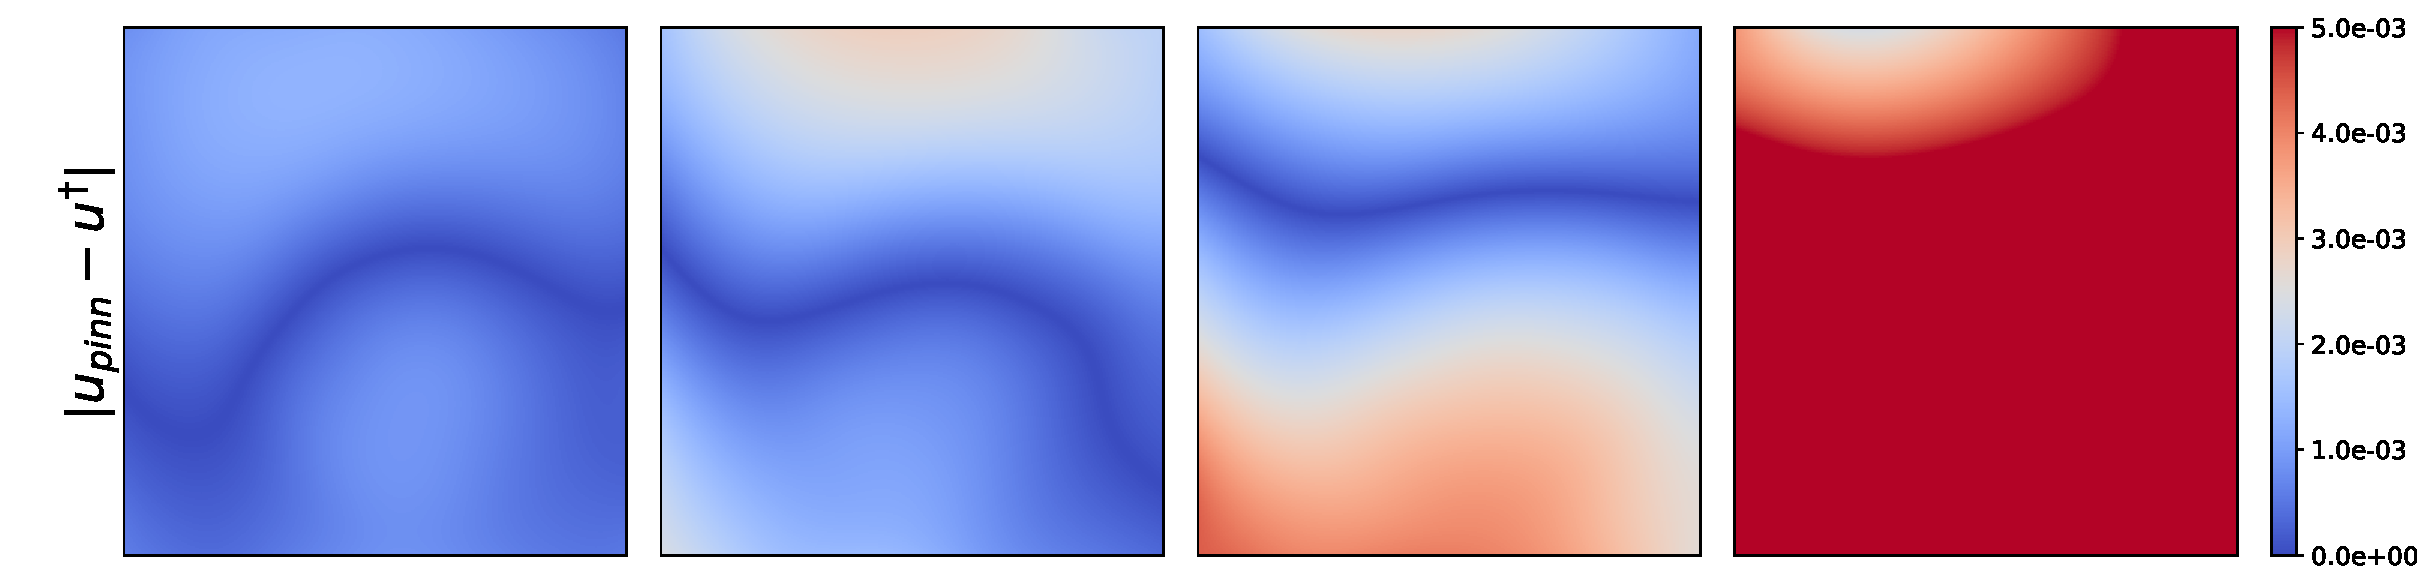
\includegraphics[width=\textwidth]{figures3/non_smooth_unn_err.eps}\par
% 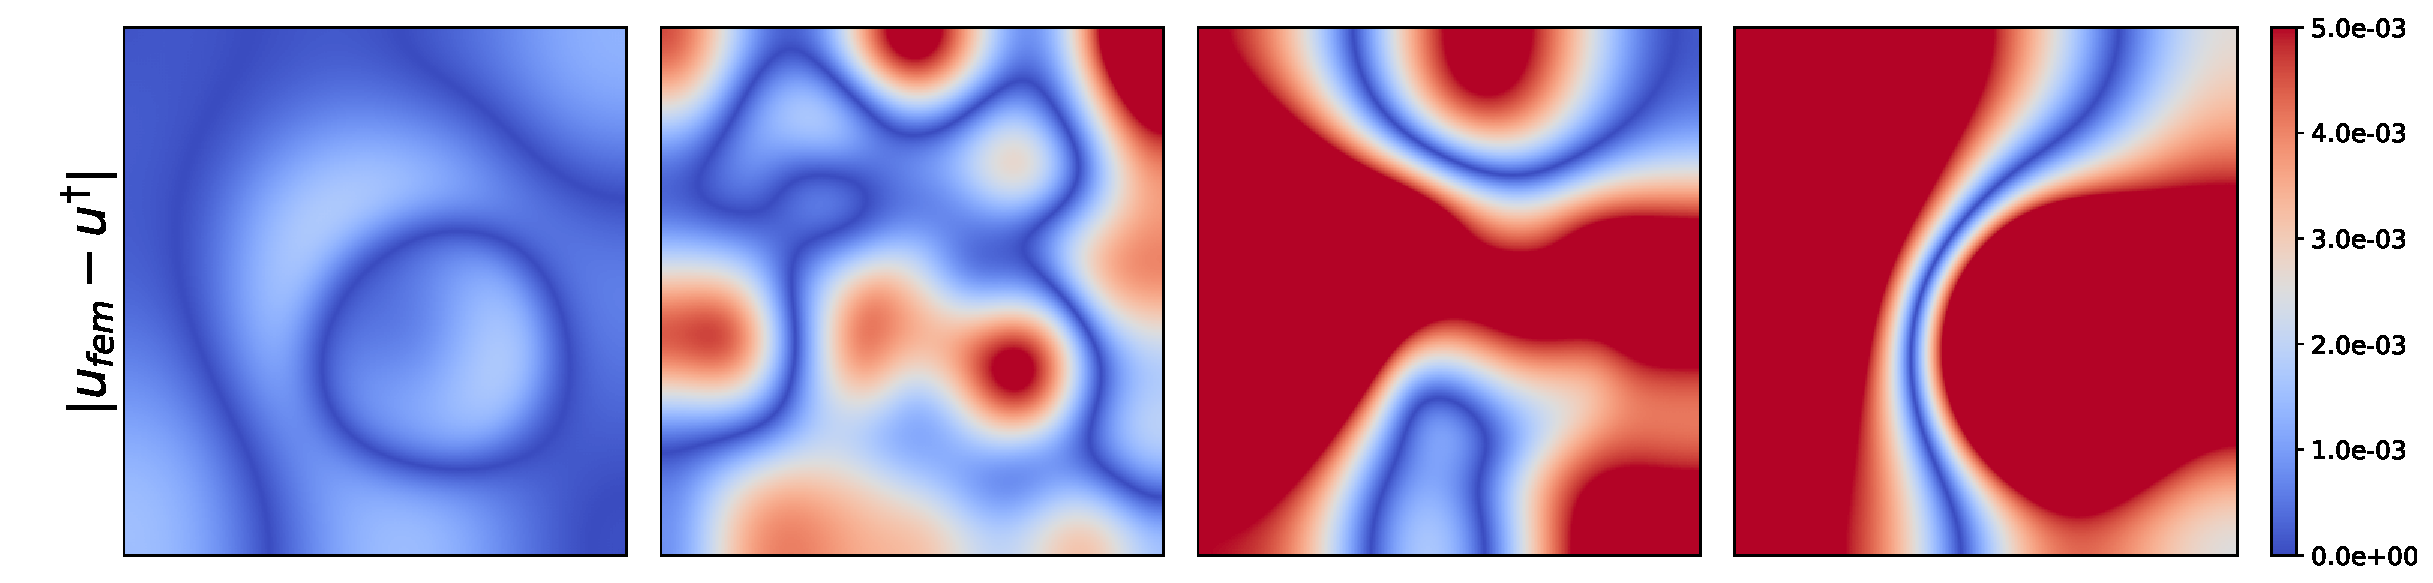
\includegraphics[width=\textwidth]{figures3/non_smooth_ufem_err.eps}
% \caption{从上到下依次为：Example \ref{example:nonsmooth} 中的真实势函数 $u^{\dagger}$，由 Tikhonov-PINNs 恢复的势函数 $u_{\text{pinn}}$，逐点绝对误差 $|u^{\dagger}-u_{\text{pinn}}|$，由 FEM 恢复的势函数 $u_{\text{fem}}$，逐点绝对误差 $|u^{\dagger}-u_{\text{fem}}|$。我们绘制了不同噪声水平下的结果。}
% \label{fig:example:nonsmooth:u}
% \end{figure}

% \begin{figure}[htbp]
% \centering
% \setlength{\abovecaptionskip}{10pt}
% 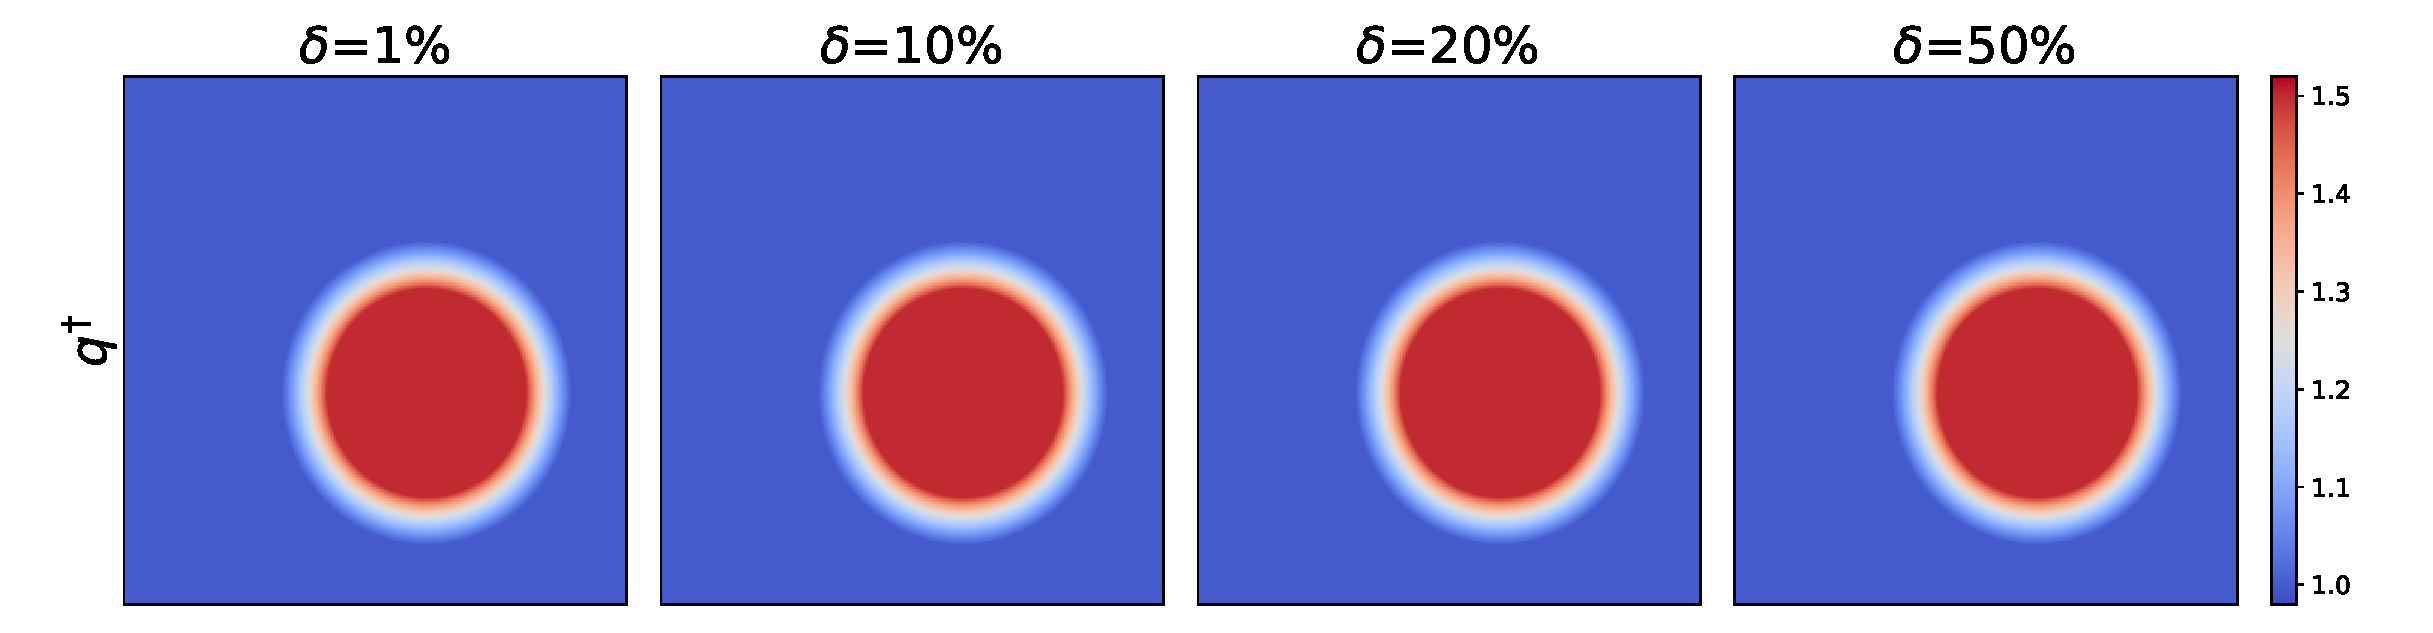
\includegraphics[width=\textwidth]{figures3/non_smooth_qdag.eps}\par
% 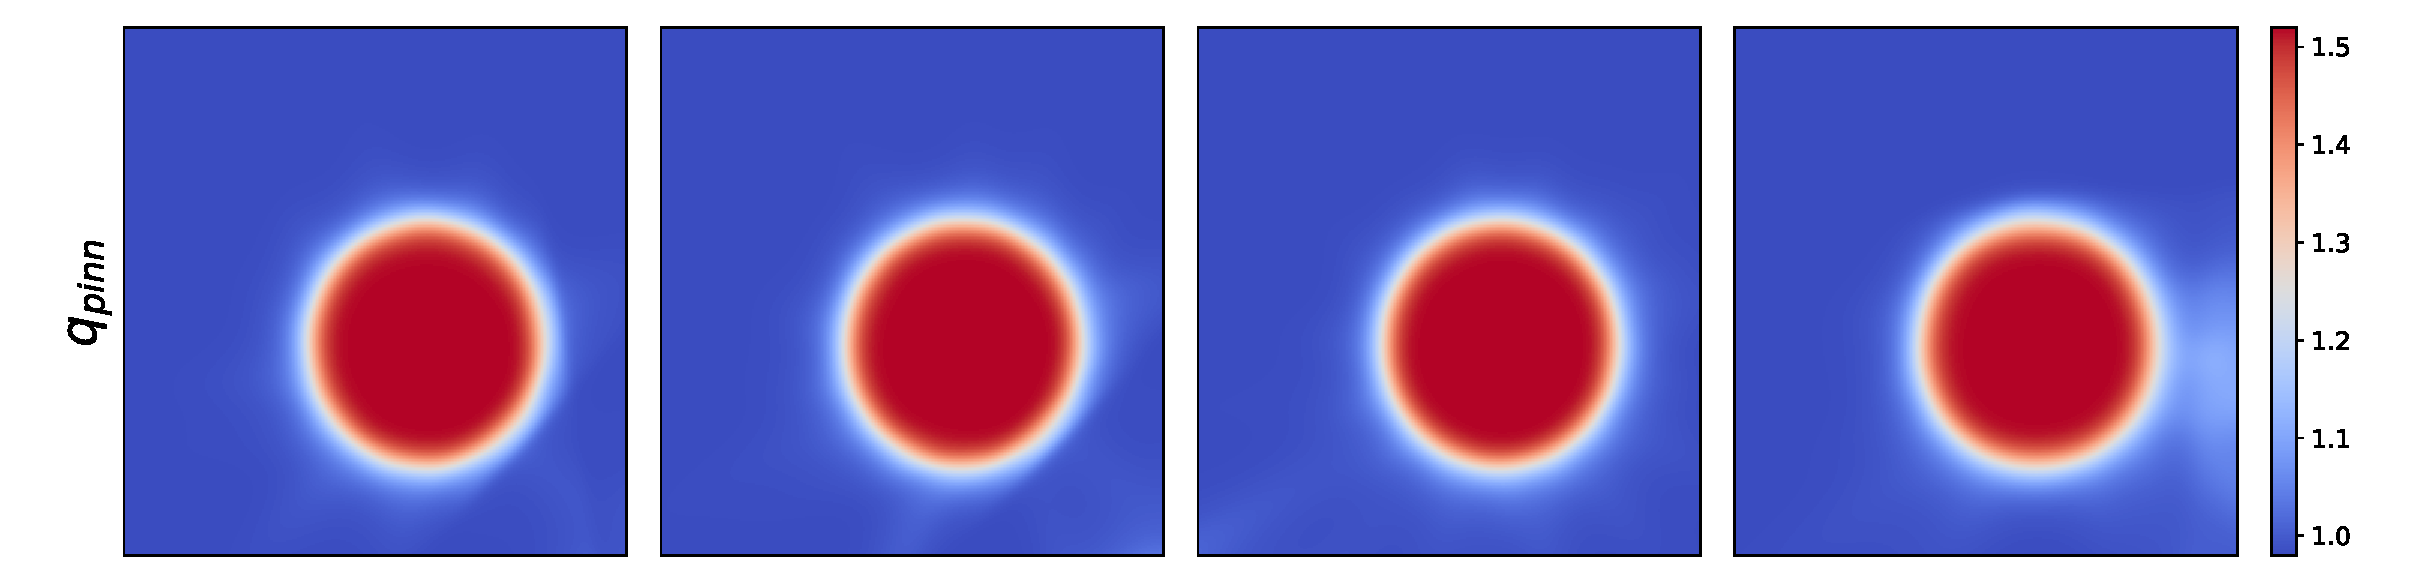
\includegraphics[width=\textwidth]{figures3/non_smooth_qnn.eps}\par
% 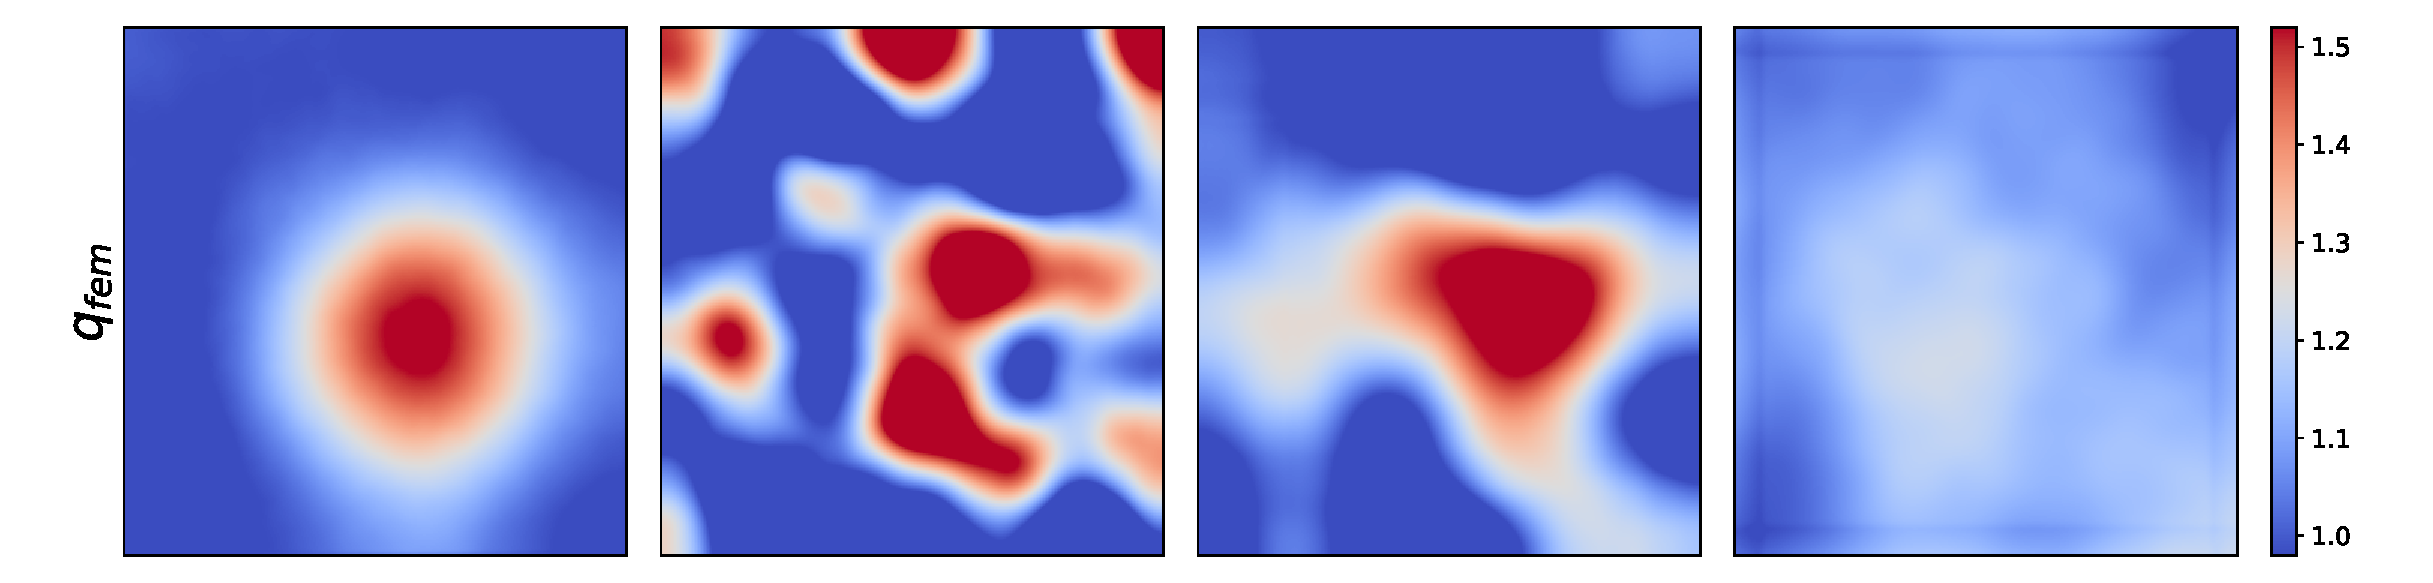
\includegraphics[width=\textwidth]{figures3/non_smooth_q_fem.eps}\par
% 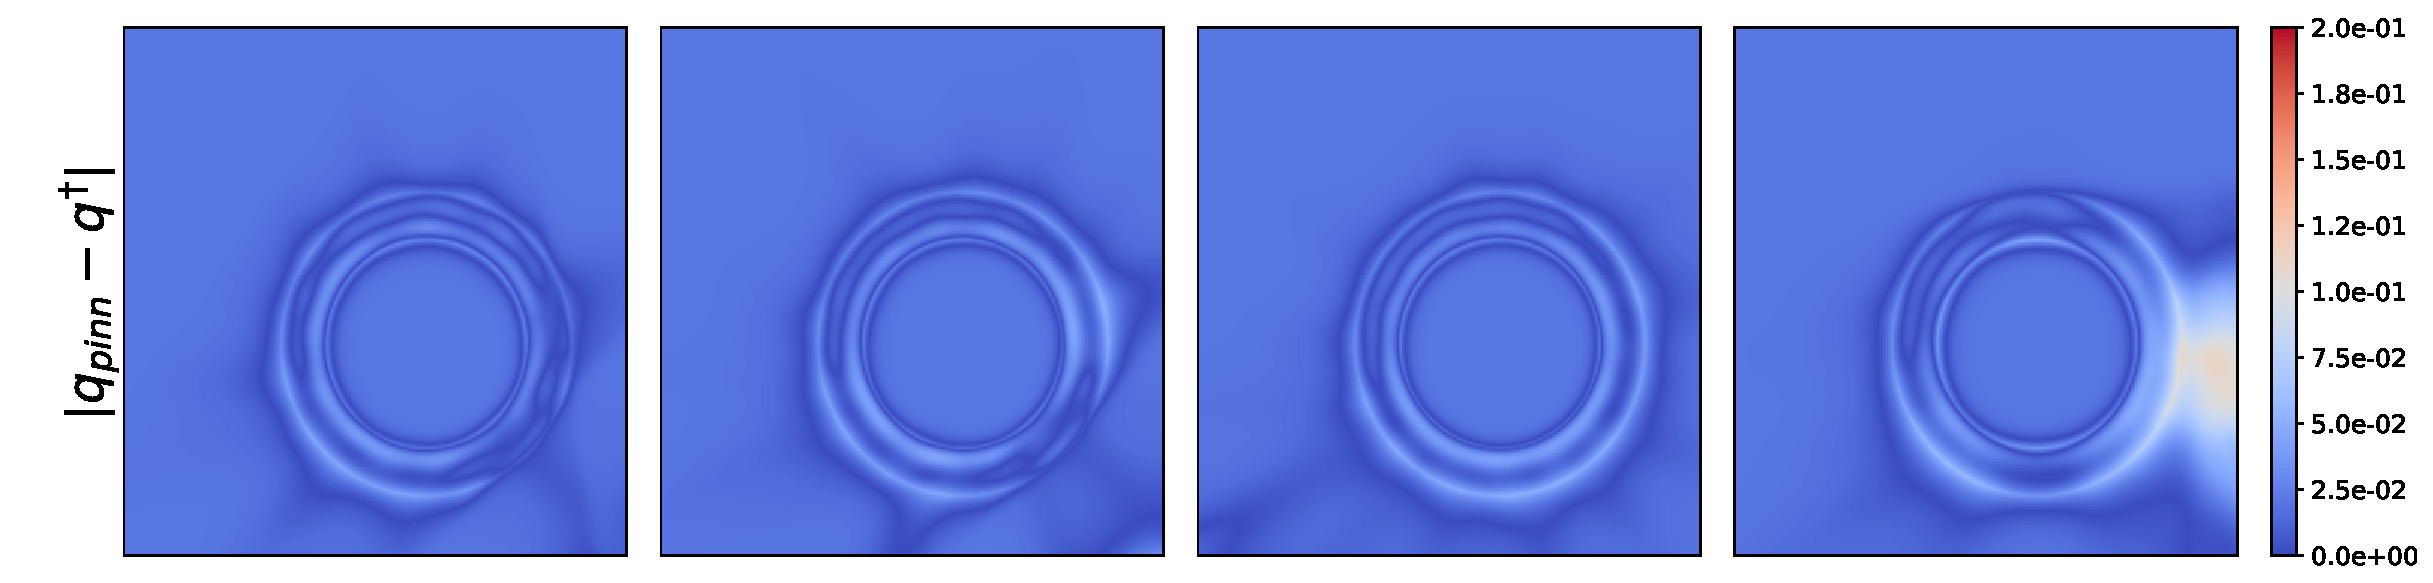
\includegraphics[width=\textwidth]{figures3/non_smooth_qnn_err.eps}\par
% 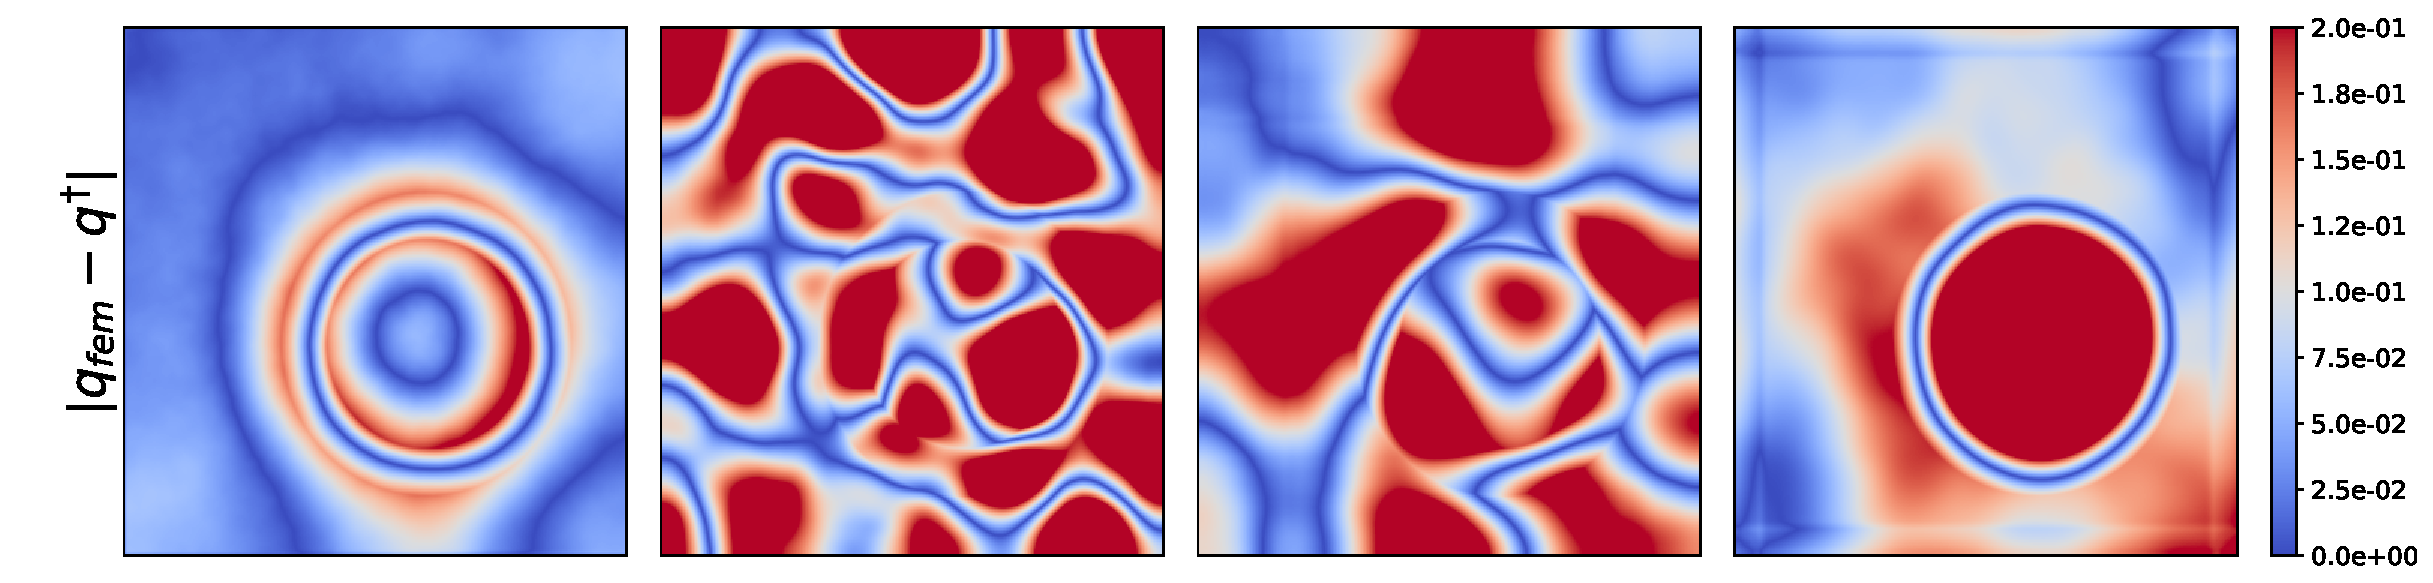
\includegraphics[width=\textwidth]{figures3/non_smooth_qfem_err.eps}
% \caption{从上到下依次为：Example \ref{example:nonsmooth} 中的真实势函数 $q^{\dagger}$，由 Tikhonov-PINNs 恢复的势函数 $q_{\text{pinn}}$，逐点绝对误差 $|q^{\dagger}-q_{\text{pinn}}|$，由 FEM 恢复的势函数 $q_{\text{fem}}$，逐点绝对误差 $|q^{\dagger}-q_{\text{fem}}|$。我们绘制了不同噪声水平下的结果。}
% \label{fig:example:nonsmooth}
% \end{figure}

% 在本例中，势函数 $q^{\dagger}$ 呈现出一种平台结构：它在红圈内部和蓝圈外部均保持常数。如图 \ref{fig:example:nonsmooth:u} 和图 \ref{fig:example:nonsmooth} 所示，重构 $u$ 相对简单，Tikhonov-PINNs 和基于有限元的方法均表现良好。然而，在重构 $q$ 时，Tikhonov-PINNs 成功捕捉到了常数值区域，而有限元方法未能精确识别 $q$ 中的界面，导致误差显著偏高。即使在高噪声水平下（例如 $\delta = 50\%$），我们的方法仍能恢复势函数的整体结构，而有限元方法几乎产生不了任何有意义的信息。

% \subsubsection{不连续问题}

% 作为第三个例子，我们将求解一个不连续势函数的反问题。
% \begin{example}\label{example:discontinuous}
% 令 $\Omega=(0,1)^{2}$ 且 $\alpha\equiv 1$。定义精确势函数 $q^{\dagger}$ 为：
% \begin{align*}
% \zeta(x_{1},x_{2})&=\exp\{-9\times(x_{1}-0.5)^{2}-9\times(x_{2}-0.5)^{2}\}, \\
% q^{\dagger}(x_{1},x_{2})&=1.0+0.5\times\zeta(x_{1},x_{2})\chi_{\{x_{1}\geq x_{2}\}},
% \end{align*}
% 精确解 $u^{\dagger}$ 为：$u^{\dagger}(x_{1},x_{2})=1+\sin(\pi x_{1})\sin(\pi x_{2})$。
% \end{example}

% \begin{table}[hbtp]
% \centering
% \footnotesize
% \caption{例 \ref{example:discontinuous} 中恢复的势函数 $\hat{q}$ 和解 $\hat{u}$ 的相对 $L^{2}$ 误差。}
% \begin{tabular}{lrrrrrr}
% \hline
% \multirow{2}[0]{*}{$\delta $ = 1\%} & \multicolumn{6}{c}{正则化参数 $\lambda$} \\
% \cline{2-7}
% & \multicolumn{1}{l}
% {$1.0\times 10^{-5}$} & 
% \multicolumn{1}{l}{$1.0\times 10^{-6}$} &
% \multicolumn{1}{l}{$1.0\times 10^{-7}$} &
% \multicolumn{1}{l}{$1.0\times 10^{-8}$} & 
%    \multicolumn{1}{l}{$1.0\times 10^{-9}$} & {0} \\
%    \hline
% $\text{err}(u_{\text{pinn}})$ & $2.05\times 10^{-3}$ & $1.54\times 10^{-3}$ & $1.07\times 10^{-3}$ & $9.83\times 10^{-4}$ & $7.55\times 10^{-4}$ & $6.42\times 10^{-4}$ \\
% $\text{err}(u_{\text{fem}})$&$1.46\times 10^{-3}$ & $7.05\times 10^{-4}$ & $4.80\times 10^{-4}$ & $2.66\times 10^{-4}$ & $2.50\times 10^{-4}$ & $2.38\times 10^{-4}$\\
% $\text{err}(q_{\text{pinn}})$ & $9.82\times 10^{-2}$ & $8.50\times 10^{-2}$ & $6.76\times 10^{-2}$ & $5.23\times 10^{-2}$ & $3.49\times 10^{-2}$ & \textbf{2.79$\times$ 10$^{-2}$} \\
% $\text{err}(q_{\text{fem}})$&$8.42\times 10^{-2}$ & $6.36\times 10^{-2}$ & $5.62\times 10^{-2}$ & $4.84\times 10^{-2}$ & $4.53\times 10^{-2}$ & $4.55\times 10^{-2}$\\
% \hline
% &       &       &       &       &       &  \\
% \hline
% \multirow{2}[0]{*}{$\delta$ = 10\%} & \multicolumn{6}{c}{正则化参数 $\lambda$} \\
% \cline{2-7}
% & $1.0\times 10^{-5}$ & $1.0\times 10^{-6}$ & $1.0\times 10^{-7}$ & $1.0\times 10^{-8}$ & $1.0\times 10^{-9}$ & \multicolumn{1}{r}{0} \\
% \hline
% $\text{err}(u_{\text{pinn}})$ & $1.96\times 10^{-3}$ & $1.74\times 10^{-3}$ & $1.38\times 10^{-3}$ & $1.12\times 10^{-3}$ & $1.49\times 10^{-3}$ & $1.48\times 10^{-3}$ \\
% $\text{err}(u_{\text{fem}})$&$1.80\times 10^{-3}$ & $9.42\times 10^{-4}$ & $1.42\times 10^{-3}$ & $1.53\times 10^{-3}$ & $1.69\times 10^{-3}$ & $1.97\times 10^{-3}$\\
% $\text{err}(q_{\text{pinn}})$ & $1.01\times 10^{-1}$ & $8.74\times 10^{-2}$ & $7.07\times 10^{-2}$ & \textbf{5.01$\times$ 10$^{-2}$} & $5.59\times 10^{-2}$ & $5.28\times 10^{-2}$ \\
% $\text{err}(q_{\text{fem}})$&$8.44\times 10^{-2}$ & $6.57\times 10^{-2}$ & $9.31\times 10^{-2}$ & $1.58\times 10^{-1}$ & $1.68\times 10^{-1}$ & $1.85\times 10^{-1}$\\
% \hline
% &       &       &       &       &       &  \\
% \hline
% \multirow{2}[0]{*}{$\delta = 20\%$} & \multicolumn{6}{c}{正则化参数 $\lambda$} \\
% \cline{2-7}
% & $1.0\times 10^{-5}$ & $1.0\times 10^{-6}$ & $1.0\times 10^{-7}$ & $1.0\times 10^{-8}$ & $1.0\times 10^{-9}$ & \multicolumn{1}{r}{0} \\
% \hline
% $\text{err}(u_{\text{pinn}})$ & $2.65\times 10^{-3}$ & $2.07\times 10^{-3}$ & $1.78\times 10^{-3}$ & $1.60\times 10^{-3}$ & $1.75\times 10^{-3}$ & $1.87\times 10^{-3}$ \\
% $\text{err}(u_{\text{fem}})$&$1.74\times 10^{-3}$ & $2.18\times 10^{-3}$ & $4.48\times 10^{-3}$ & $3.91\times 10^{-3}$ & $4.67\times 10^{-3}$ & $3.08\times 10^{-3}$\\
% $\text{err}(q_{\text{pinn}})$ & $1.05\times 10^{-1}$ & $9.18\times 10^{-2}$ & $7.22\times 10^{-2}$ & \textbf{6.50$\times$ 10$^{-2}$} & $7.20\times 10^{-2}$ & $7.73\times 10^{-2}$ \\
% $\text{err}(q_{\text{fem}})$&$8.58\times 10^{-2}$ & $9.39\times 10^{-2}$ & $2.35\times 10^{-1}$ & $2.00\times 10^{-1}$ & $6.43\times 10^{-1}$ & $1.89\times 10^{-1}$\\
% \hline
% &       &       &       &       &       &  \\
% \hline
% \multirow{2}[0]{*}{$\delta = 50\%$} & \multicolumn{6}{c}{正则化参数 $\lambda$} \\
% \cline{2-7}
% & $1.0\times 10^{-5}$ & $1.0\times 10^{-6}$ & $1.0\times 10^{-7}$ & $1.0\times 10^{-8}$ & $1.0\times 10^{-9}$ & \multicolumn{1}{r}{0} \\
% \hline
% $\text{err}(u_{\text{pinn}})$ & $3.92\times 10^{-3}$ & $4.57\times 10^{-3}$ & $4.33\times 10^{-3}$ & $4.23\times 10^{-3}$ & $4.21\times 10^{-3}$ & $4.35\times 10^{-3}$ \\
% $\text{err}(u_{\text{fem}})$&$4.99\times 10^{-3}$ & $7.18\times 10^{-3}$ & $8.53\times 10^{-3}$ & $8.25\times 10^{-3}$ & $1.29\times 10^{-2}$ & $1.01\times 10^{-2}$\\
% $\text{err}(q_{\text{pinn}})$ & $1.21\times 10^{-1}$ & $1.04\times 10^{-1}$ & $8.50\times 10^{-2}$ & $8.08\times 10^{-2}$ & \textbf{8.04$\times$ 10$^{-2}$} & $1.06\times 10^{-1}$ \\
% $\text{err}(q_{\text{fem}})$&$1.08\times 10^{-1}$ & $2.27\times 10^{-1}$ & $5.12\times 10^{-1}$ & $4.62\times 10^{-1}$ & $5.90\times 10^{-1}$ & $8.28\times 10^{-1}$\\
% \hline
% \end{tabular}
% \label{tab:discontinuous}
% \end{table}

% \begin{figure}[htbp]
% \centering
% \setlength{\abovecaptionskip}{10pt}
% 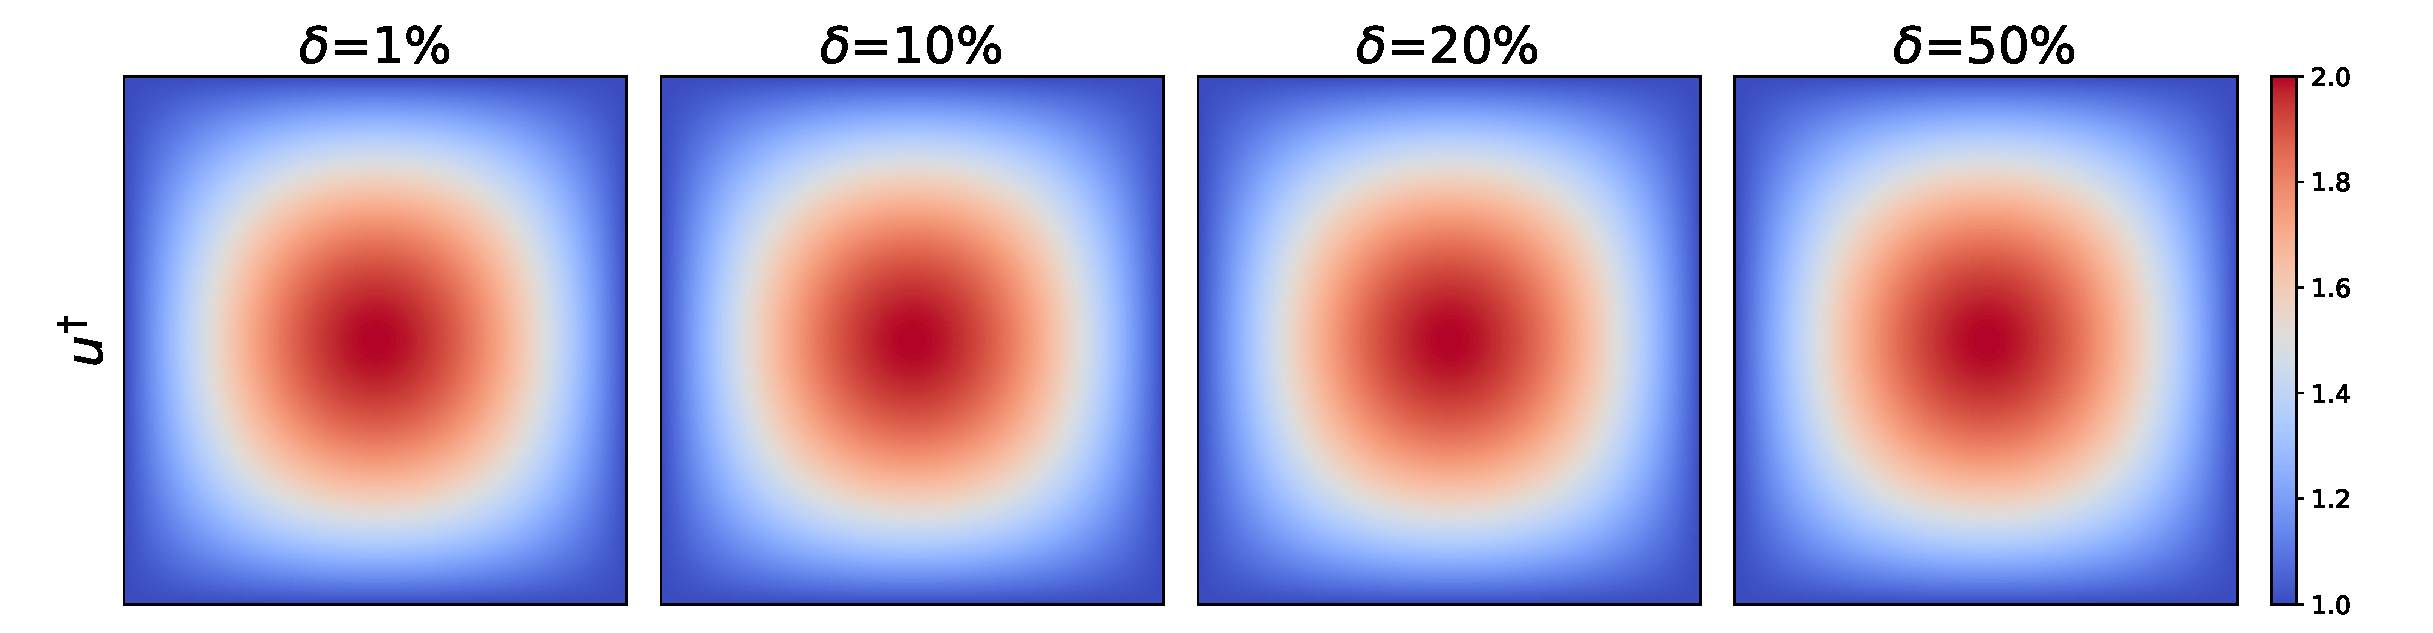
\includegraphics[width=\textwidth]{figures3/discontinuous_udag.eps}\par
% 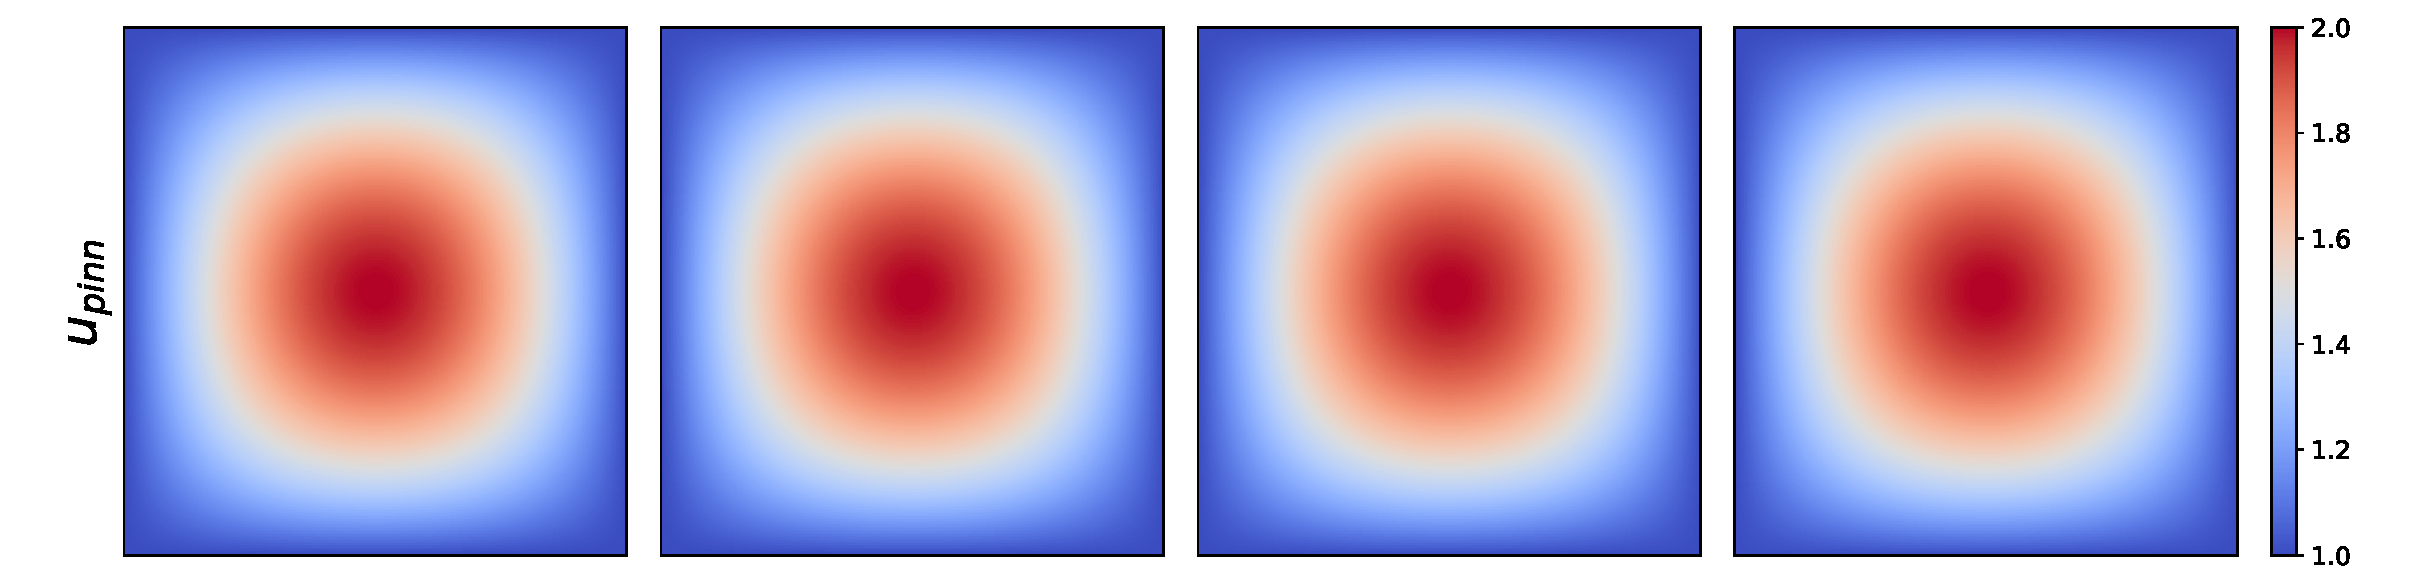
\includegraphics[width=\textwidth]{figures3/discontinuous_unn.eps}\par
% 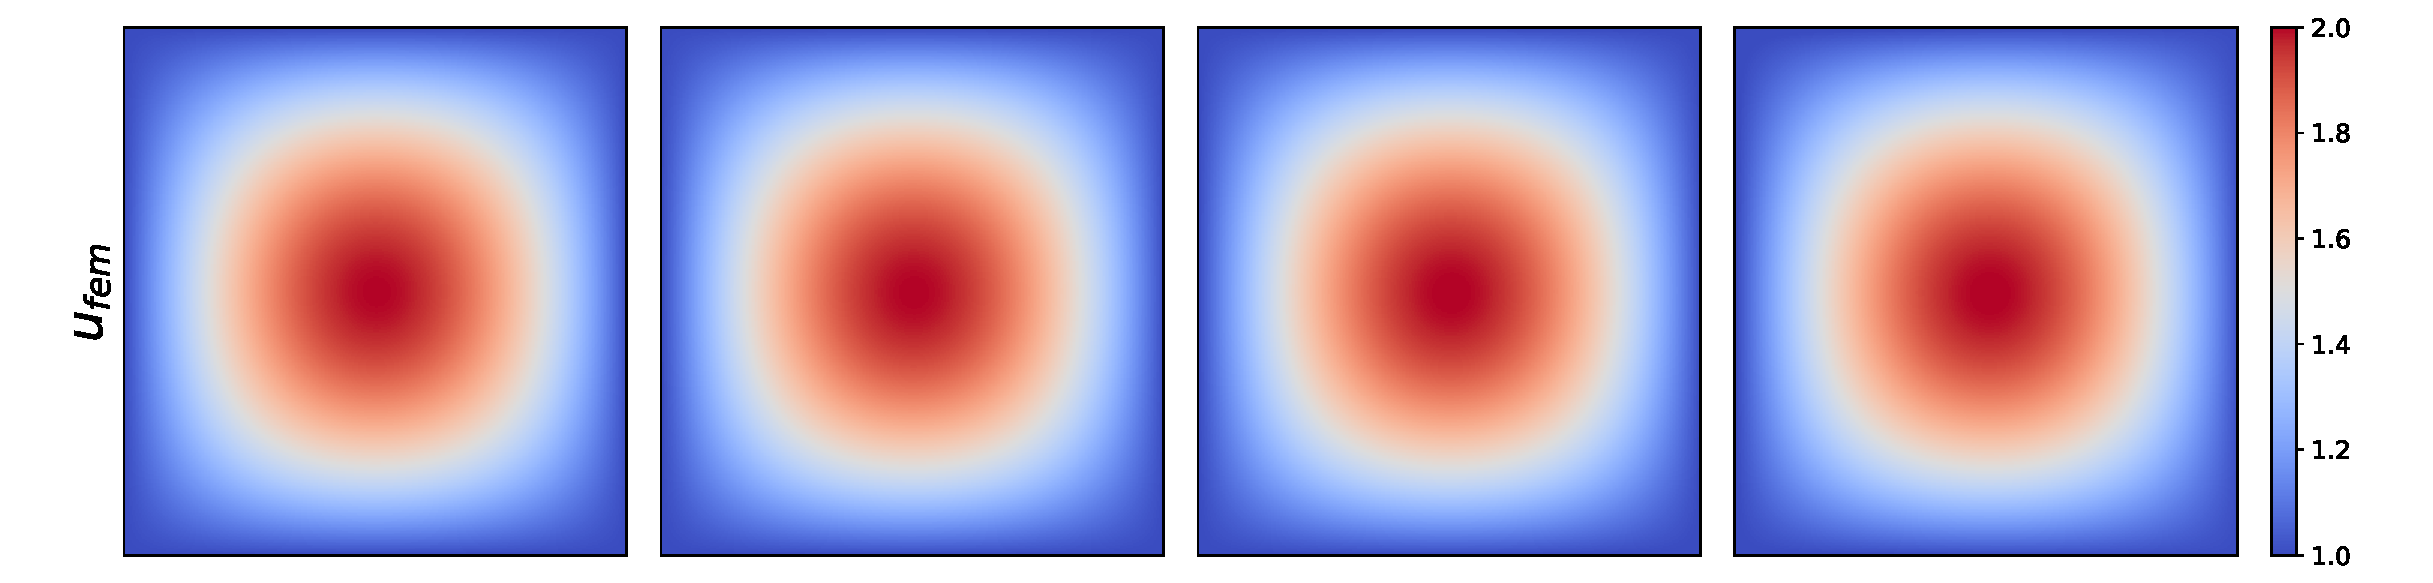
\includegraphics[width=\textwidth]{figures3/discontinuous_ufem.eps}\par
% 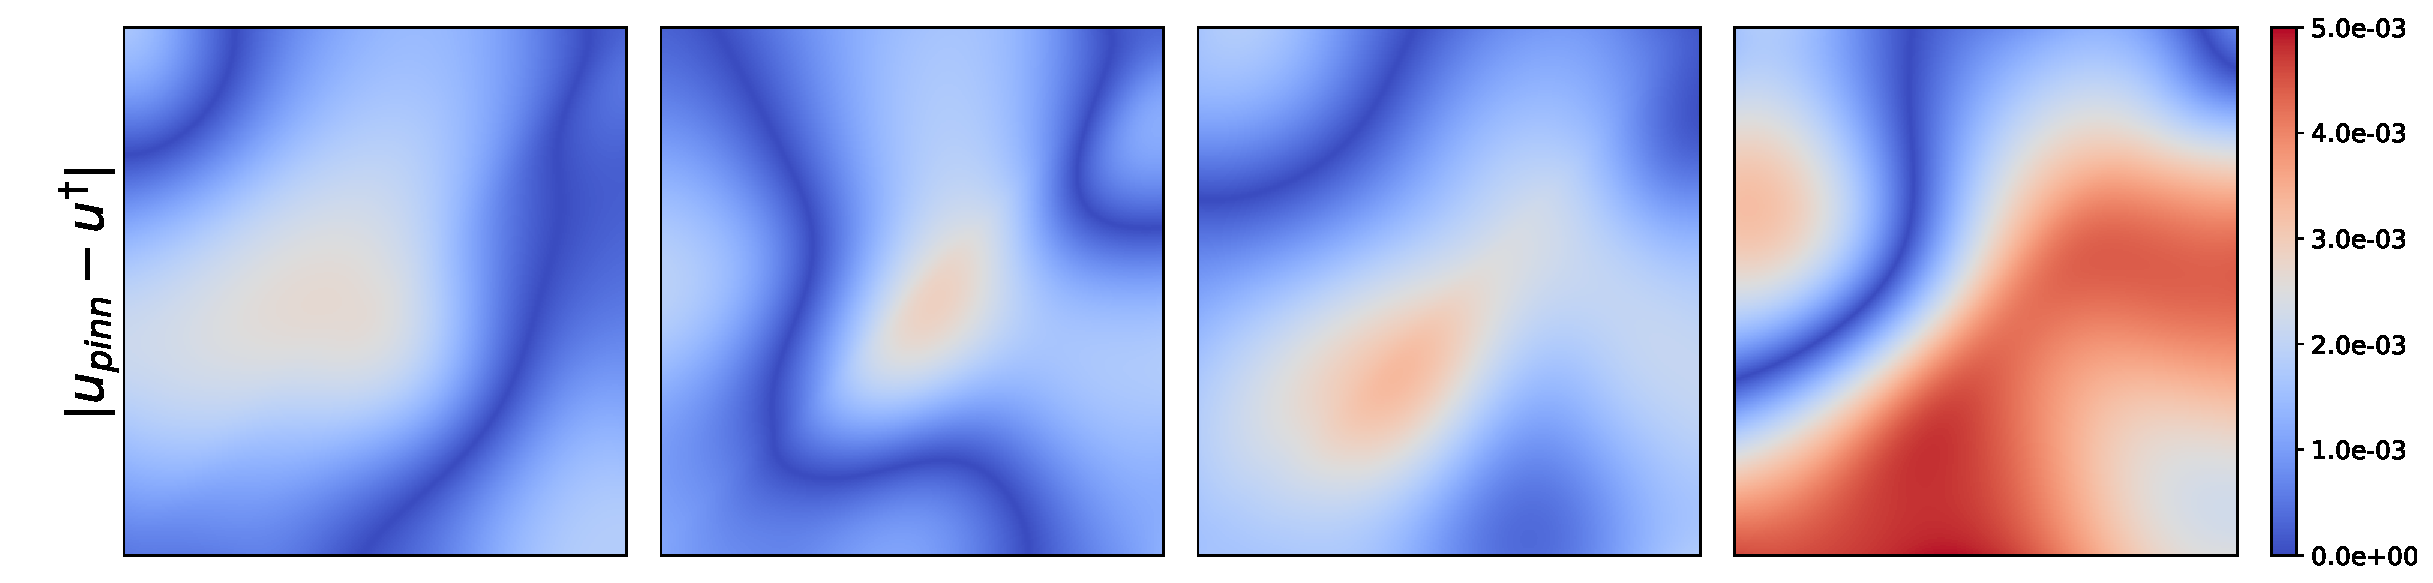
\includegraphics[width=\textwidth]{figures3/discontinuous_unn_err.eps}\par
% 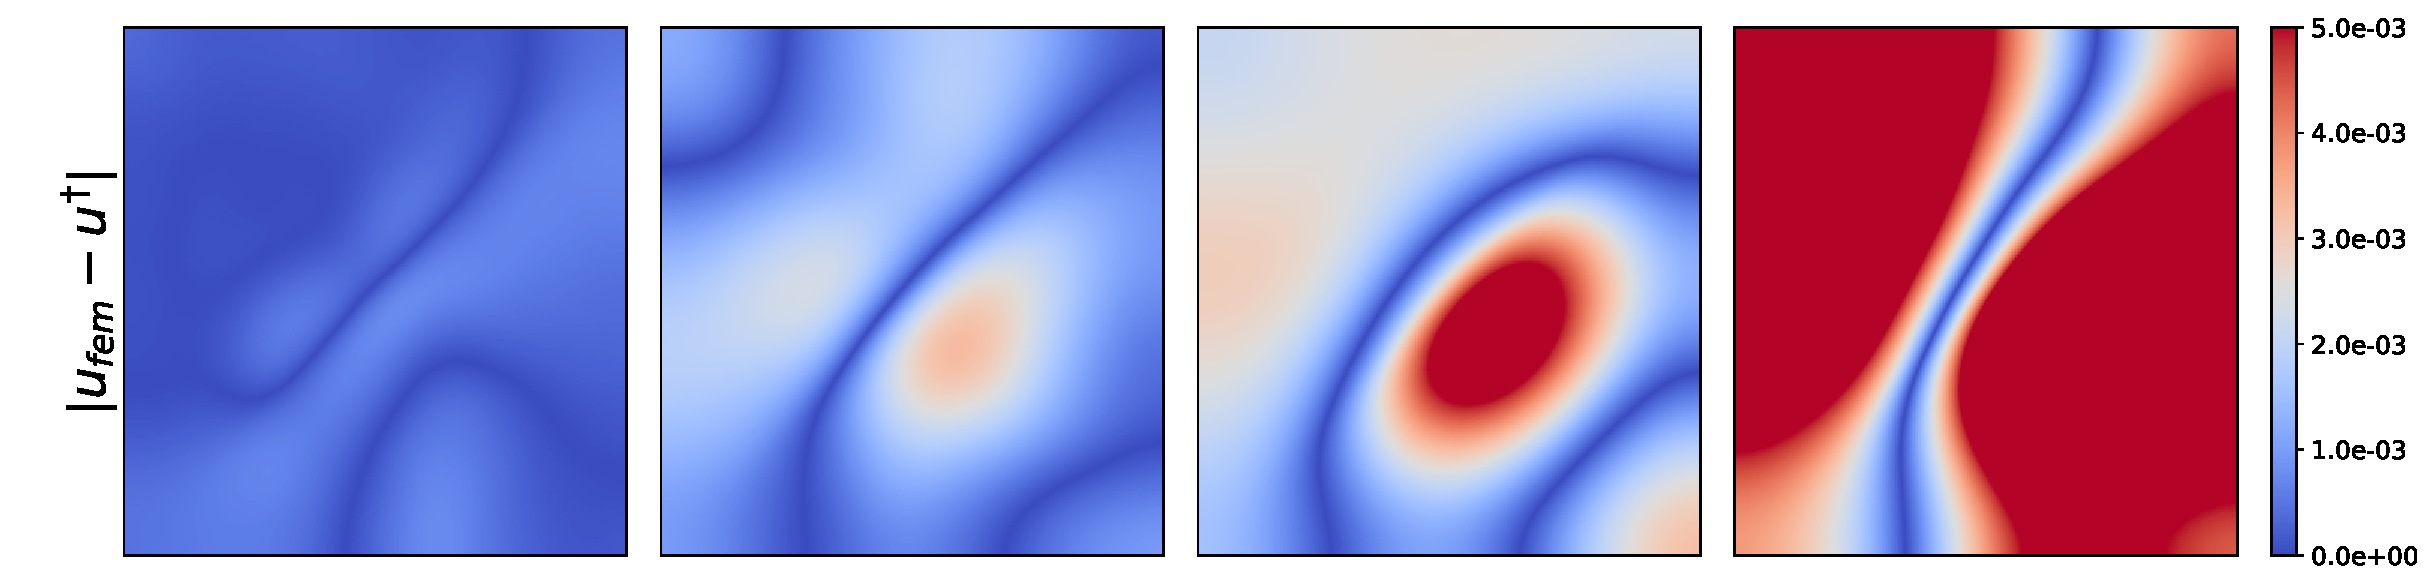
\includegraphics[width=\textwidth]{figures3/discontinuous_ufem_err.eps}
% \caption{从上到下依次为：例 \ref{example:discontinuous} 中的真实解 $u^{\dagger}$，Tikhonov-PINNs 恢复的解 $u_{\text{pinn}}$，逐点绝对误差 $|u^{\dagger}-u_{\text{pinn}}|$，FEM 恢复的解 $u_{\text{fem}}$，以及逐点绝对误差 $|u^{\dagger}-u_{\text{fem}}|$。我们绘制了在不同噪声水平下的结果。}
% \label{fig:example:discontinuous:u}
% \end{figure}

% \begin{figure}[htbp]
% \centering
% \setlength{\abovecaptionskip}{10pt}
% 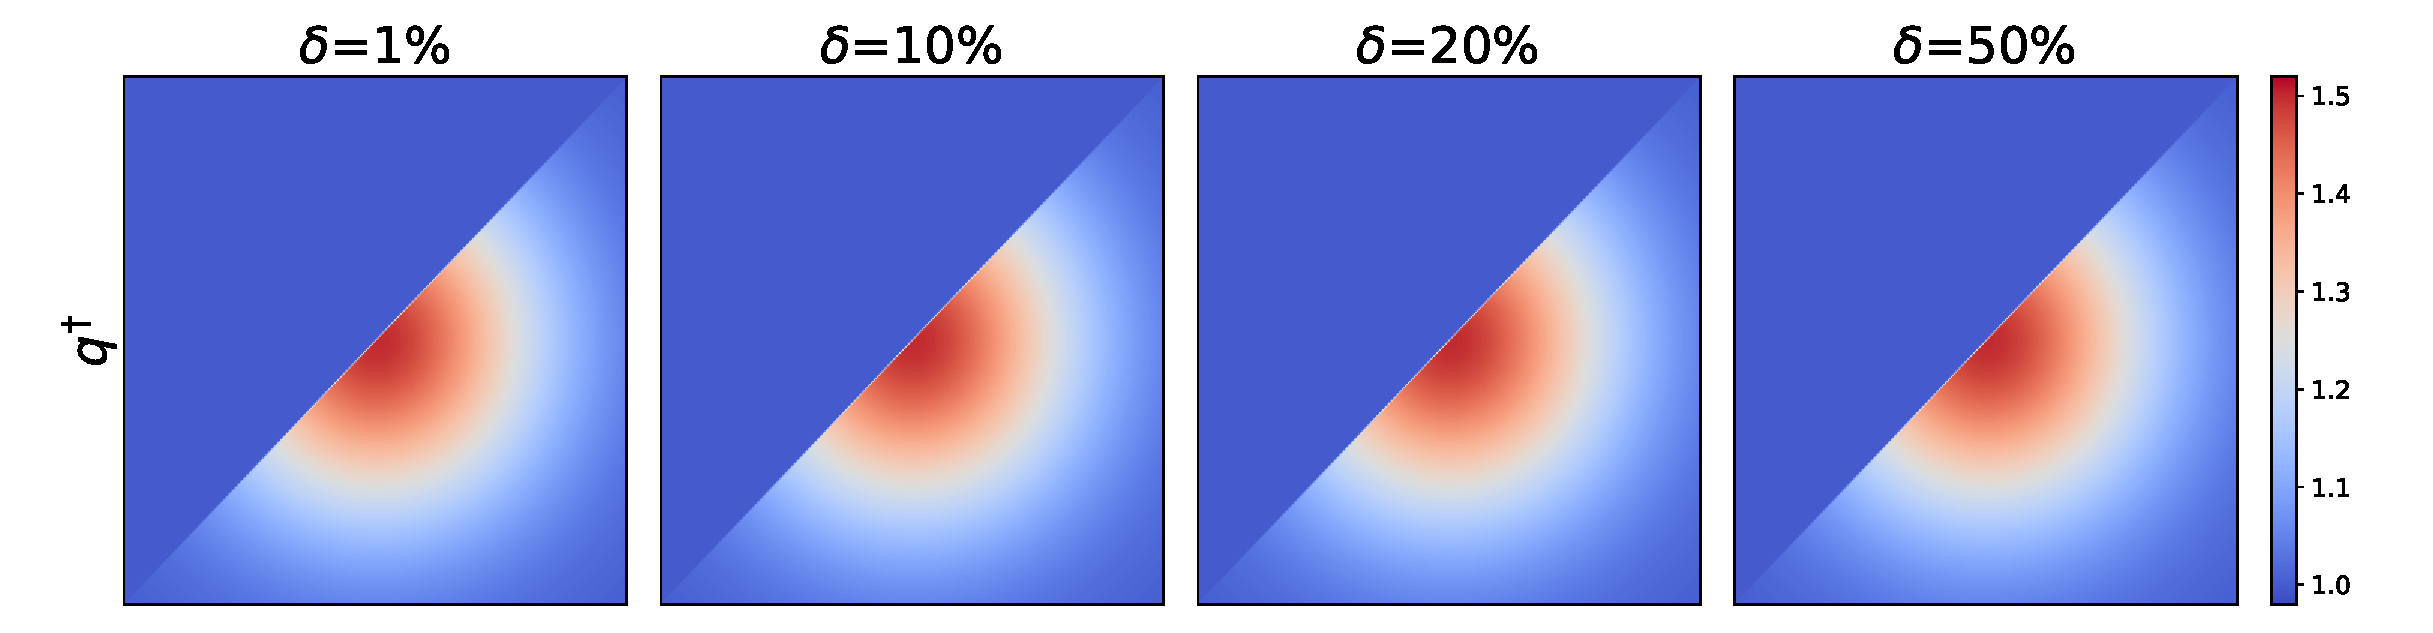
\includegraphics[width=\textwidth]{figures3/discontinuous_qdag.eps}\par
% 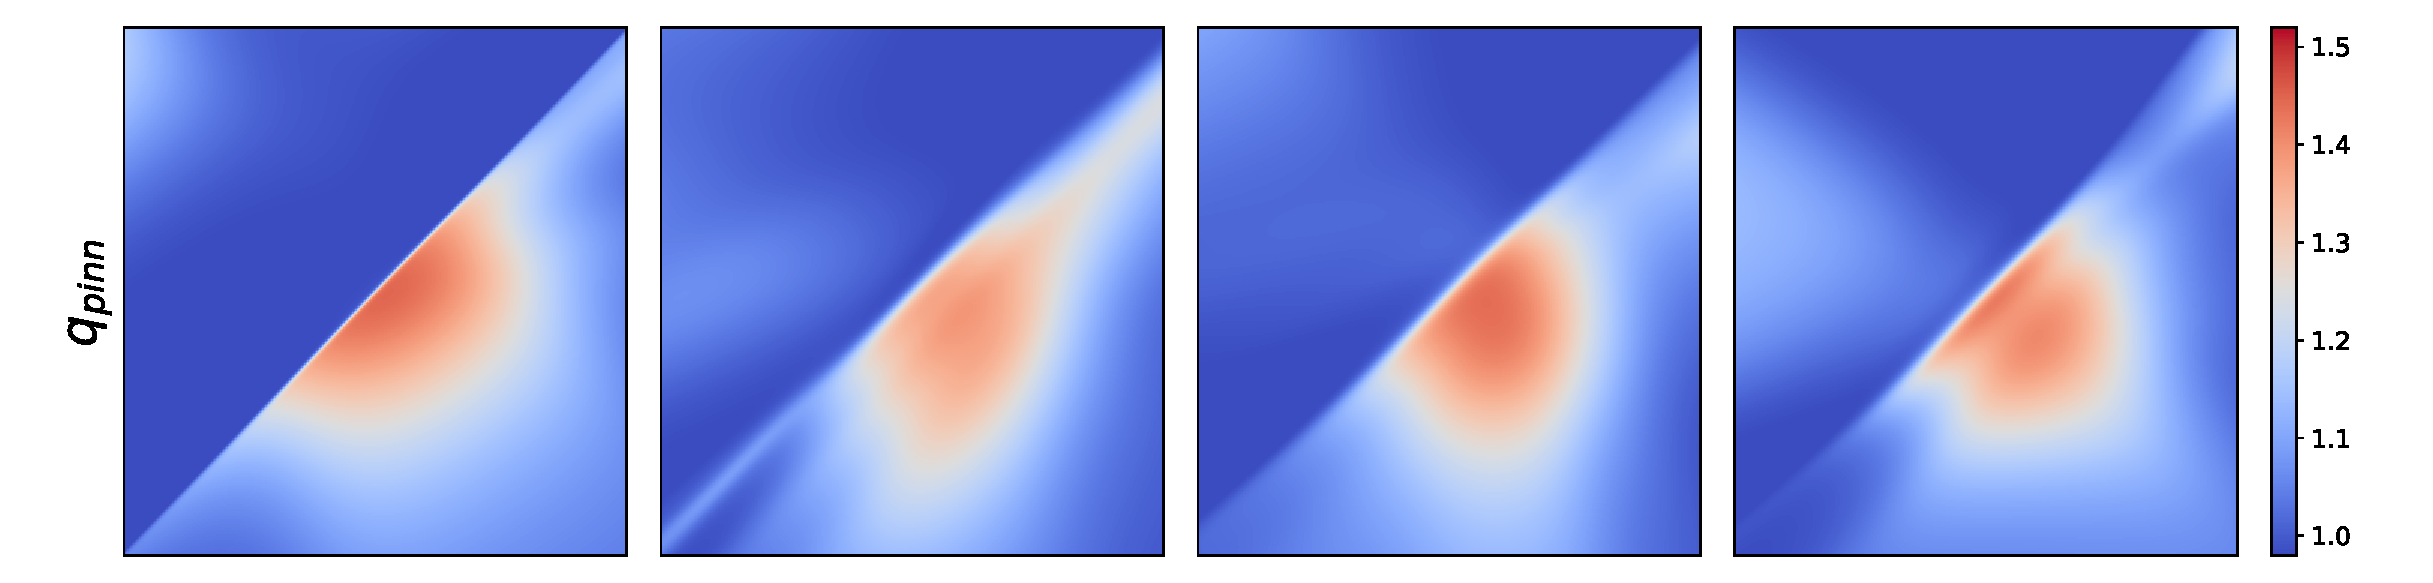
\includegraphics[width=\textwidth]{figures3/discontinuous_qnn.eps}\par
% 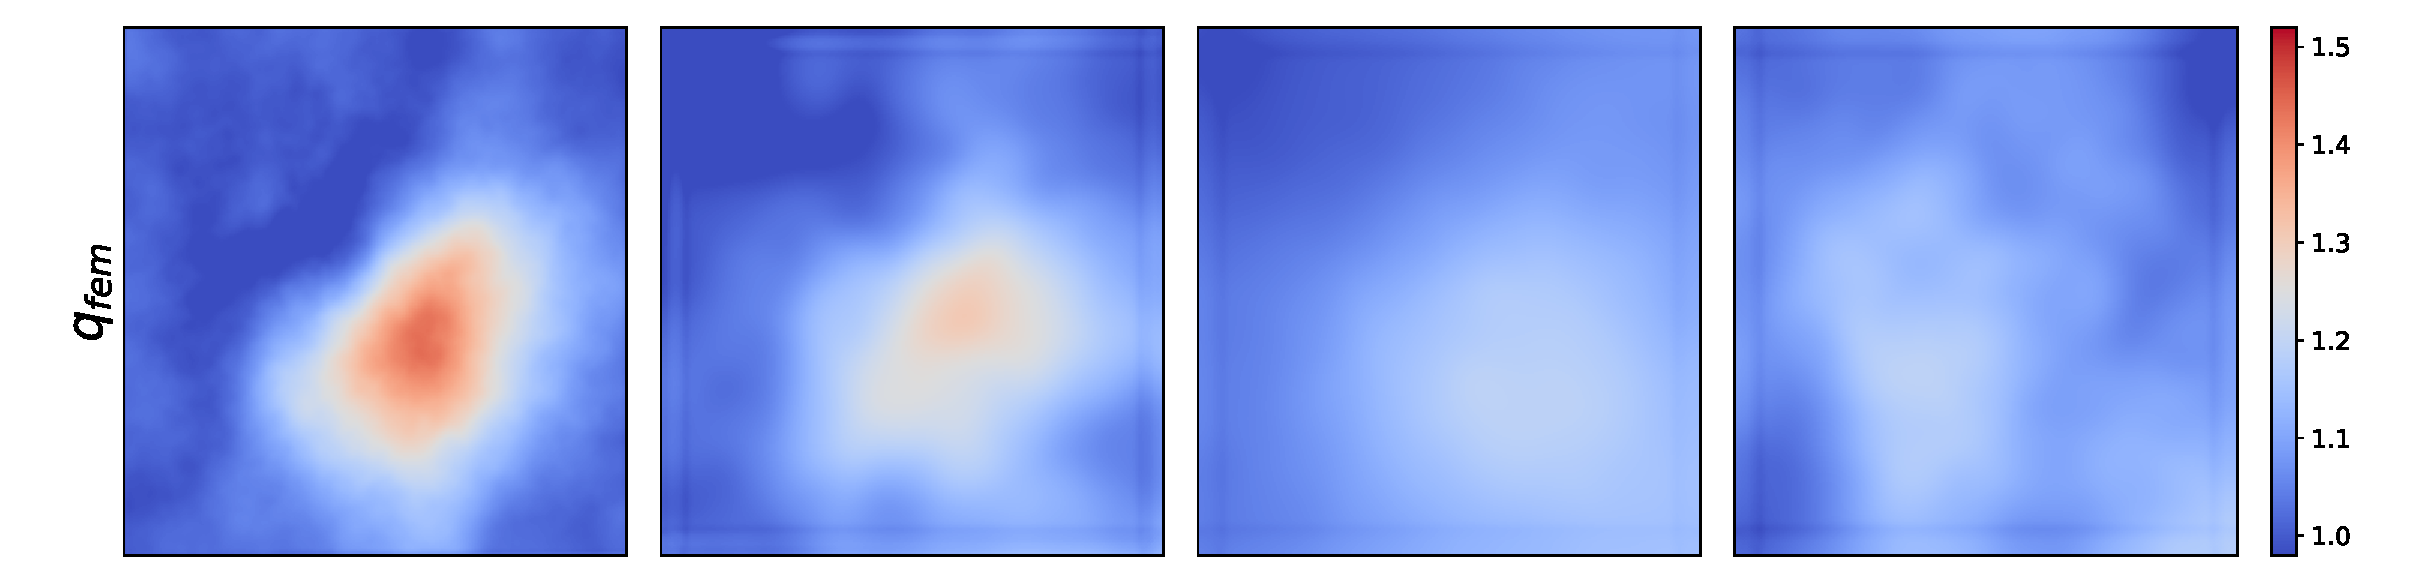
\includegraphics[width=\textwidth]{figures3/discontinuous_q_fem.eps}\par
% 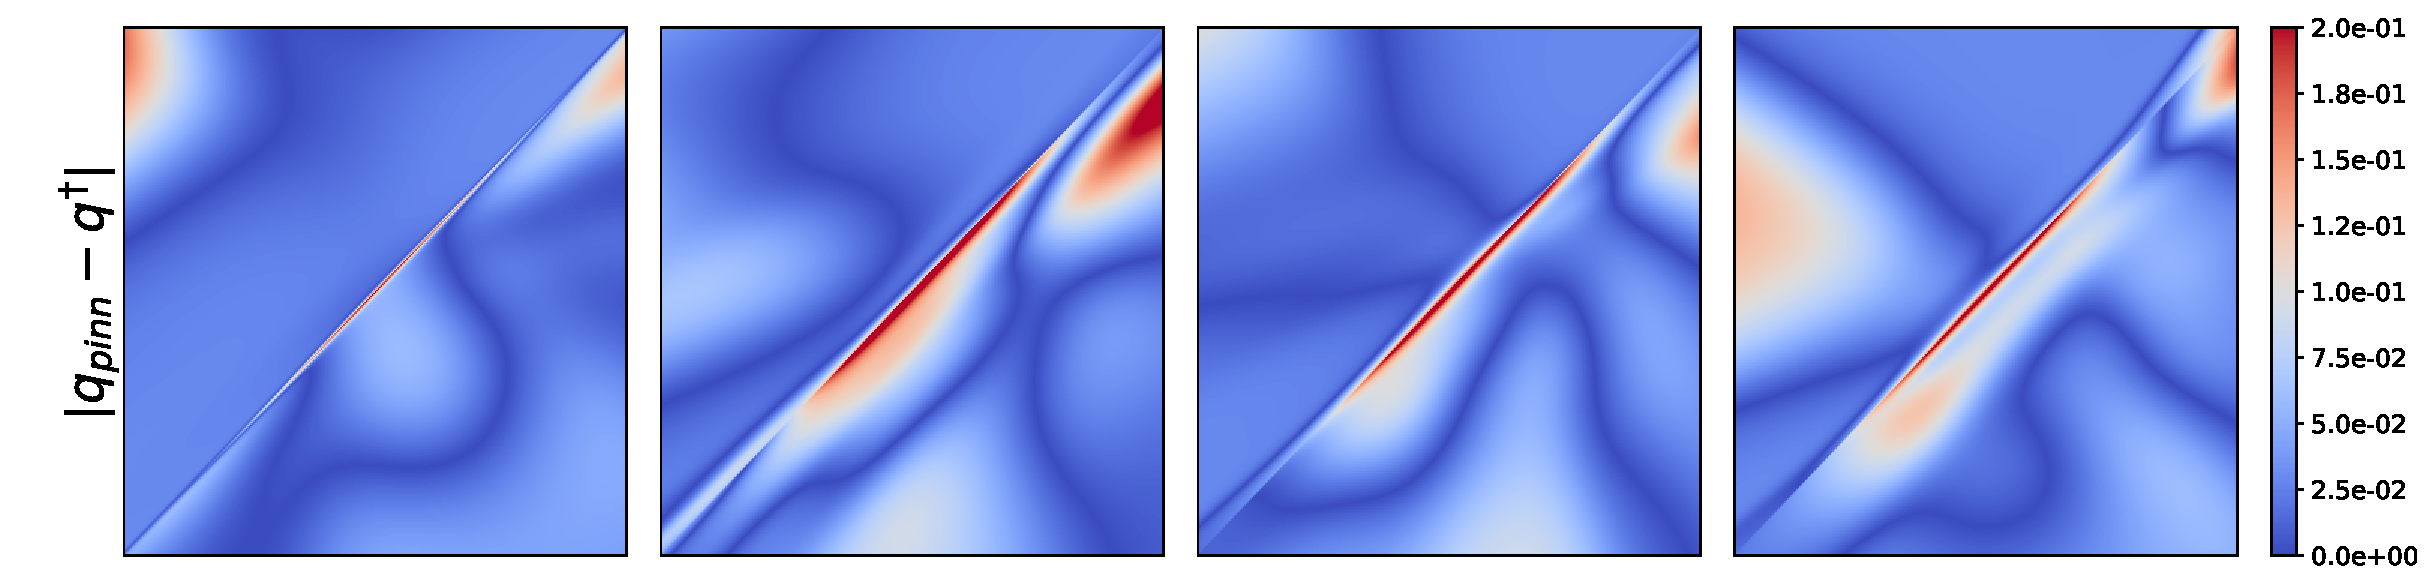
\includegraphics[width=\textwidth]{figures3/discontinuous_qnn_err.eps}\par
% 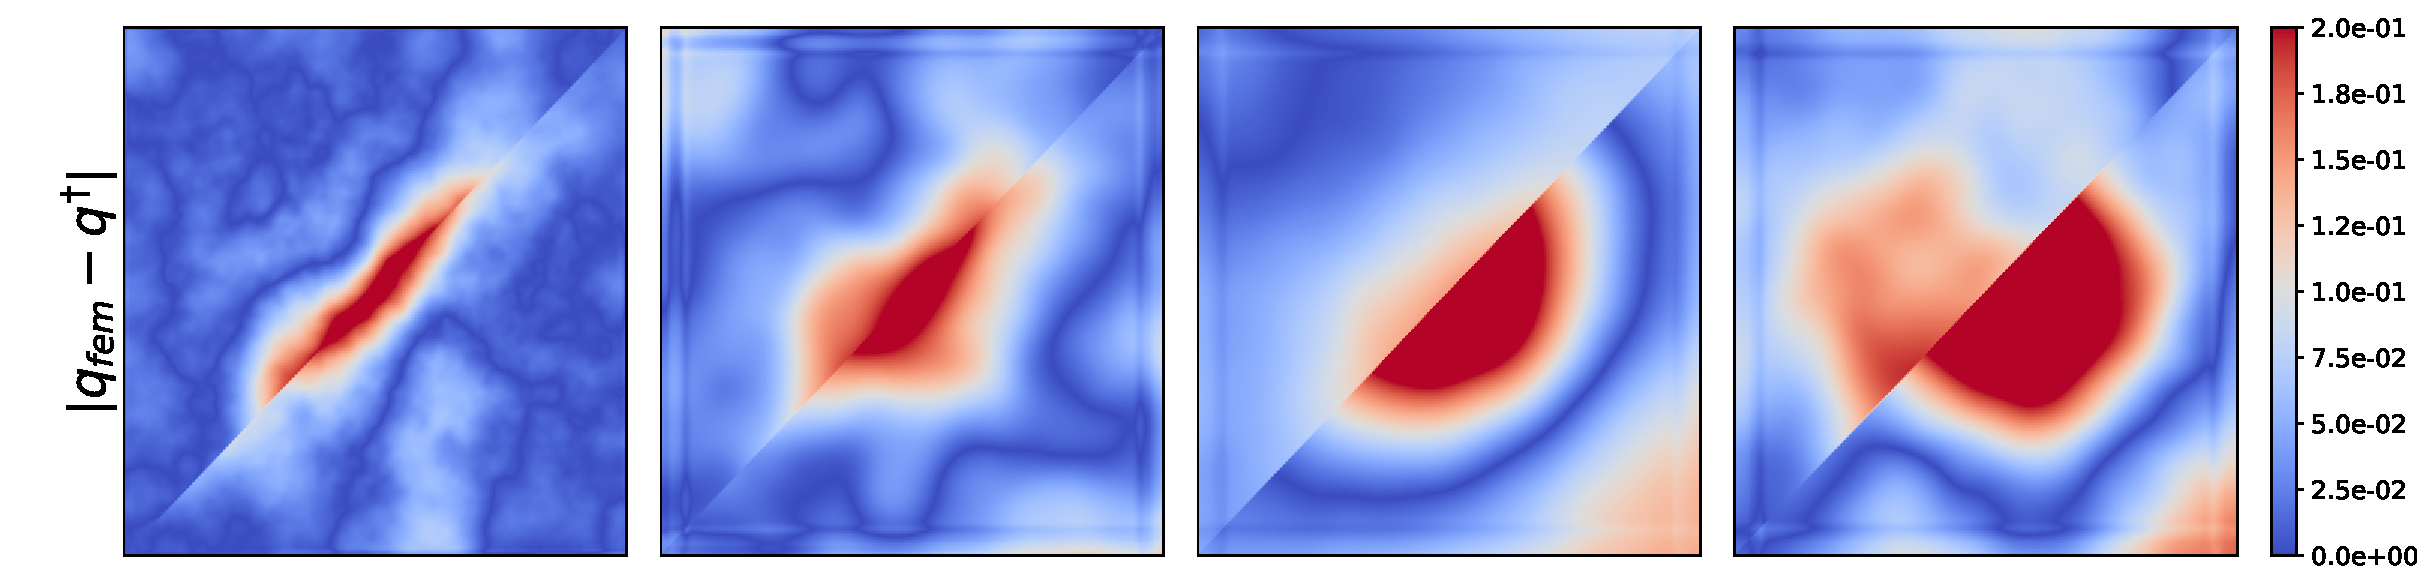
\includegraphics[width=\textwidth]{figures3/discontinuous_qfem_err.eps}
% \caption{从上到下依次为：例 \ref{example:discontinuous} 中的真实势函数 $q^{\dagger}$，Tikhonov-PINNs 恢复的势函数 $q_{\text{pinn}}$，逐点绝对误差 $|q^{\dagger}-q_{\text{pinn}}|$，FEM 恢复的势函数 $q_{\text{fem}}$，以及逐点绝对误差 $|q^{\dagger}-q_{\text{fem}}|$。我们绘制了在不同噪声水平下的结果。}
% \label{fig:example:discontinuous}
% \end{figure}

% 根据构造，势函数 $q$ 沿对角线 $x=y$ 呈现不连续性，这进一步加剧了反问题的不适定性。如图~\ref{fig:example:discontinuous:u} 和图~\ref{fig:example:discontinuous} 所示，Tikhonov-PINNs 能够在所有噪声水平下捕捉到这种不连续性。相比之下，有限元方法无法识别不连续区域，仅能在 1\% 的噪声水平下粗略定位高势区域。如表 \ref{tab:discontinuous} 所示，Tikhonov-PINNs 在所有噪声水平下对 $q$ 的相对误差均达到 $\calO(10^{-2})$ 左右，通常比有限元方法优越一个数量级。

% 还应注意，在上述实验中，当 $\lambda$ 非零时，Tikhonov-PINNs 通常能获得最优解（参见表 \ref{tab:discontinuous}）。这一观察结果部分说明了损失函数中的 Tikhonov 正则化对于提升标准 PINNs 方法的性能至关重要。

% \subsection{高维问题}
% 由于其无网格的特性，基于神经网络的方法可以很容易地扩展到高维问题，并在一定程度上缓解维数灾难。在本小节中，依照 \cite{jin2023conductivity} 中算例 5.4 的设置，我们将 Tikhonov-PINNs 应用于一个五维问题，这是传统有限元方法难以实现的场景。

% \begin{example}\label{example:highdim}
% 令 $\Omega=(0,1)^{5}$ 且 $\alpha\equiv 1$。我们考虑识别如下势函数：
% \begin{equation*}
% \begin{array}{rcl}
% q^{\dagger}(x)&=&1-(x_1-0.5)^2-(x_2-0.5)^2\\
% &{}&+\cos(\pi(x_3+1.5))+\cos(\pi (x_4+1.5))+\cos(\pi (x_5+1.5)),
% \end{array}
% \end{equation*}
% 准确解 $u^{\dagger}$ 为 $u^{\dagger}(x)=\sum_{i=1}^{5}(x_{i}+\frac{1}{3}x_{i}^3)$。
% \end{example}


% \begin{figure}
% \centering
% \setlength{\abovecaptionskip}{10pt}
% 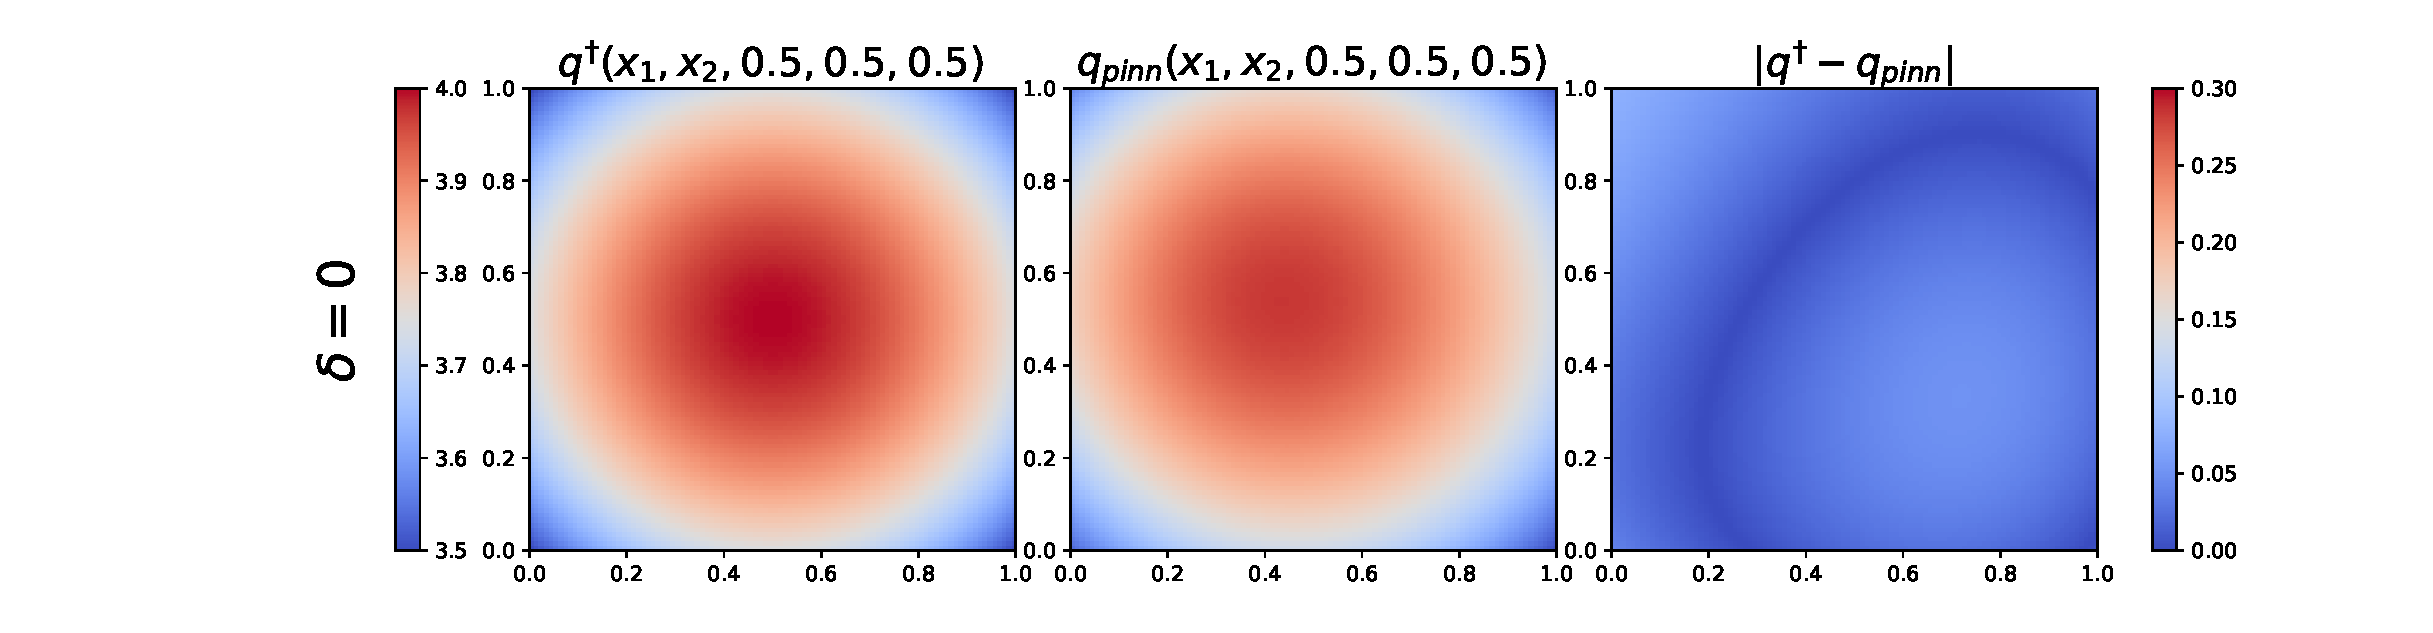
\includegraphics[width=\textwidth]{figures3/ex_5_00.eps}\par
% 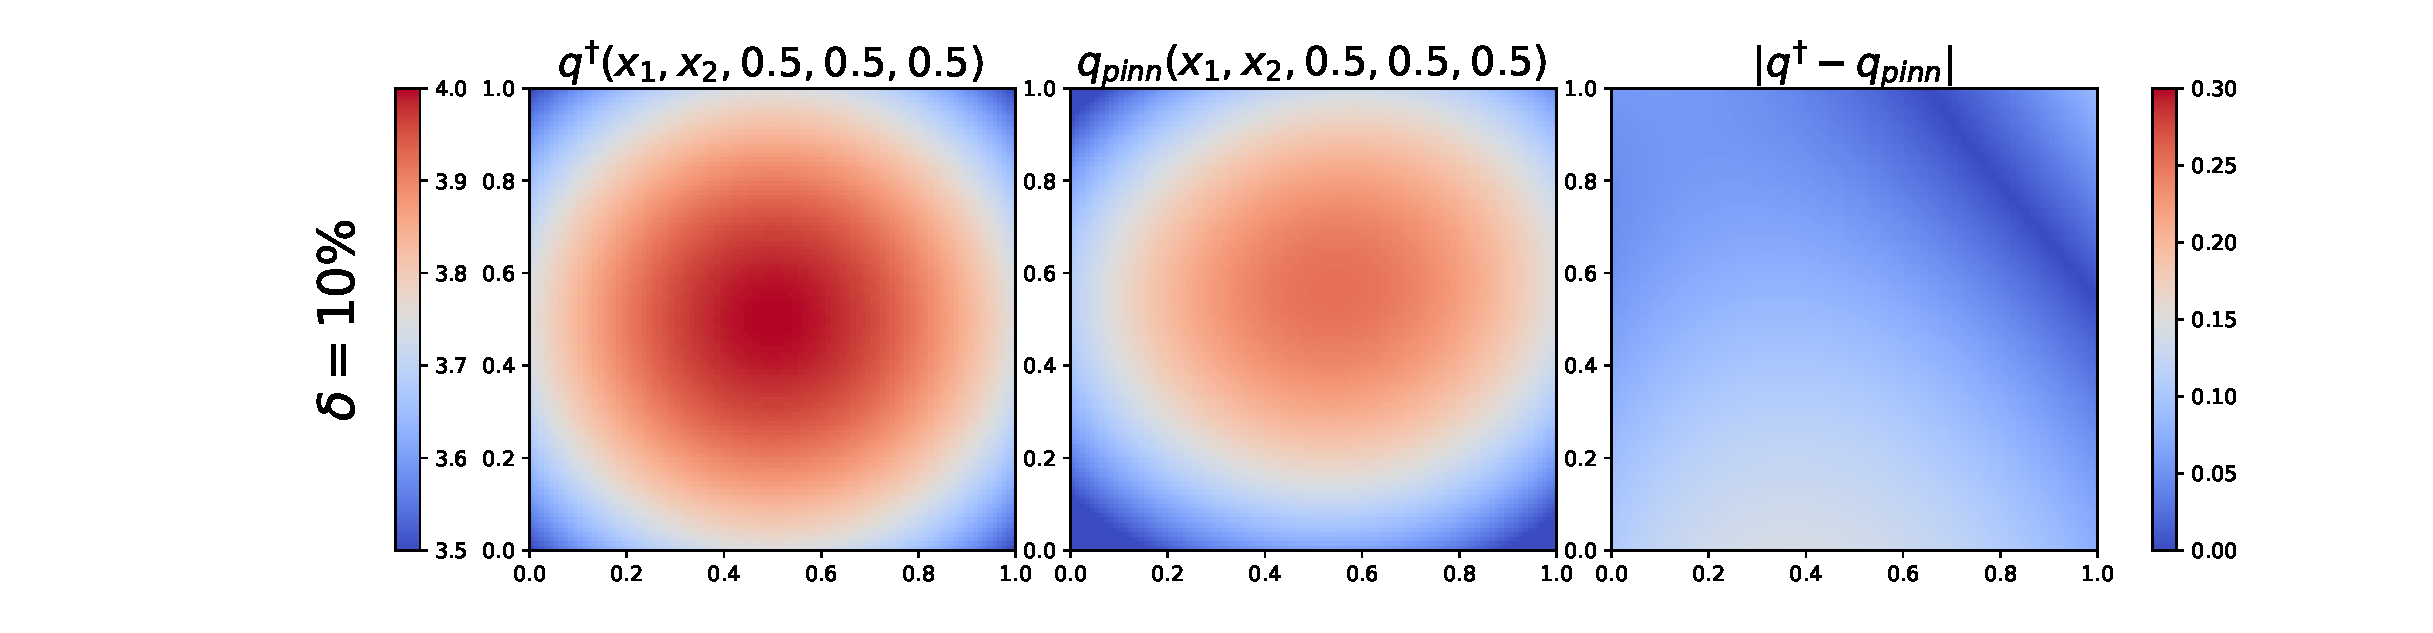
\includegraphics[width=\textwidth]{figures3/ex_5_10.eps}\par
% \caption{算例 \ref{example:highdim} 在切片 $x_3=x_4=x_5=0.5$ 上的真实解与 Tikhonov-PINNs 解。第一行对应 $\delta=0$ 的情况，而第二行展示了 $\delta=10\%$ 的情况。}
% \label{fig:example:highdim}
% \end{figure}

% \begin{table}[hbtp]
% \centering
% \caption{算例 \ref{example:highdim} 中恢复的势 $\hat{q}$ 和解 $\hat{u}$ 的相对 $L^{2}$ 误差。}
% \begin{tabular}{crrrr}
% \hline
% 正则化参数 $\lambda$ & $1.0\times 10^{-7}$ & $1.0\times 10^{-8}$ & $1.0\times 10^{-9}$ & $0$ \\
% \hline
% $\text{err}(u_{\text{pinn}})(\delta=0)$ & $1.09\times 10^{-3}$ & $1.14\times 10^{-3}$ & $1.05\times 10^{-3}$ & $1.39\times 10^{-3}$ \\
% $\text{err}(q_{\text{pinn}})(\delta=0)$ & $3.14\times 10^{-2}$ & $3.08\times 10^{-2}$ & \textbf{3.07$\times$ 10$^{-2}$} & $3.09\times 10^{-2}$  \\
% $\text{err}(u_{\text{pinn}})(\delta=10\%)$ & $4.21\times 10^{-3}$ & $4.19\times 10^{-3}$ & $4.19\times 10^{-3}$ & $4.18\times 10^{-3}$  \\
% $\text{err}(q_{\text{pinn}})(\delta=10\%)$ & $4.33\times 10^{-2}$ & $4.25\times 10^{-2}$ & \textbf{4.24$\times$ 10$^{-2}$} & \textbf{4.24$\times$ 10$^{-2}$}  \\
% \hline
% \end{tabular}
% \label{tab:highdim}
% \end{table}

% 在实验中，我们使用了一个包含 4 个隐藏层且宽度为 26 的神经网络。我们在内部采样了 60,000 个点，在边界上采样了 60,000 个点。模型使用 Adam 优化器训练了 50,000 次迭代，学习率为 $10^{-4}$, 权重衰减系数为 $10^{-9}$。

% 算法误差结果总结在表 \ref{tab:highdim} 中。此外，我们对 $x_{3}=x_{4}=x_{5}=0.5$ 处的切片进行了可视化，如图~\ref{fig:example:highdim} 所示。结果表明，Tikhonov-PINNs 在解决这一五维问题时依然有效，能够准确逼近解和潜在的势函数。

\subsection{缓解半收敛现象}\label{sec:semi_converge}
众所周知，半收敛现象经常出现在不适定反问题中 \cite{engl1996regularization}。在优化的早期阶段，迭代解逐渐逼近真实解。然而，随着迭代的进行，数据噪声的放大导致解偏离真实解，从而导致误差增加。正如 Figure~\ref{fig:err_q} 所示，对于算例 5.3，基于有限元的方法的重构误差最初下降，但随后显著上升，特别是在高噪声水平下。相比之下，Tikhonov-PINNs 有效地缓解了这一问题。我们方法的误差随着迭代次数的增加平滑且持续地下降，没有表现出明显的上升。半收敛的存在使得必须使用早停法来获得最优解，这降低了方法的鲁棒性并限制了可达到的精度。相比之下，Tikhonov-PINNs 固有的优势使其对噪声不那么敏感，允许更多的迭代，最终产生更准确的重构结果。

此外，我们也可以使用算例 5.3 来比较计算成本。在求解算例 5.3 的单次迭代中，Tikhonov-PINNs 平均需要 1.91 秒，而基于 FEM 的方法需要 2.04 秒。如图 10 所示，经过 120 次迭代（229.2 秒）后，Tikhonov-PINNs 在约 $10^6$ 个采样点下达到了约 $O(10^{-2})$ 的精度。相比之下，基于 FEM 的方法进行 120 次迭代需要 244.8 秒，达到的精度为 $O(10^{-1})$。这些结果凸显了 Tikhonov-PINNs 在精度和计算效率方面的明显优势，特别是对于不连续问题。

\begin{figure}[htbp]
   \centering
   \setlength{\abovecaptionskip}{10pt}
   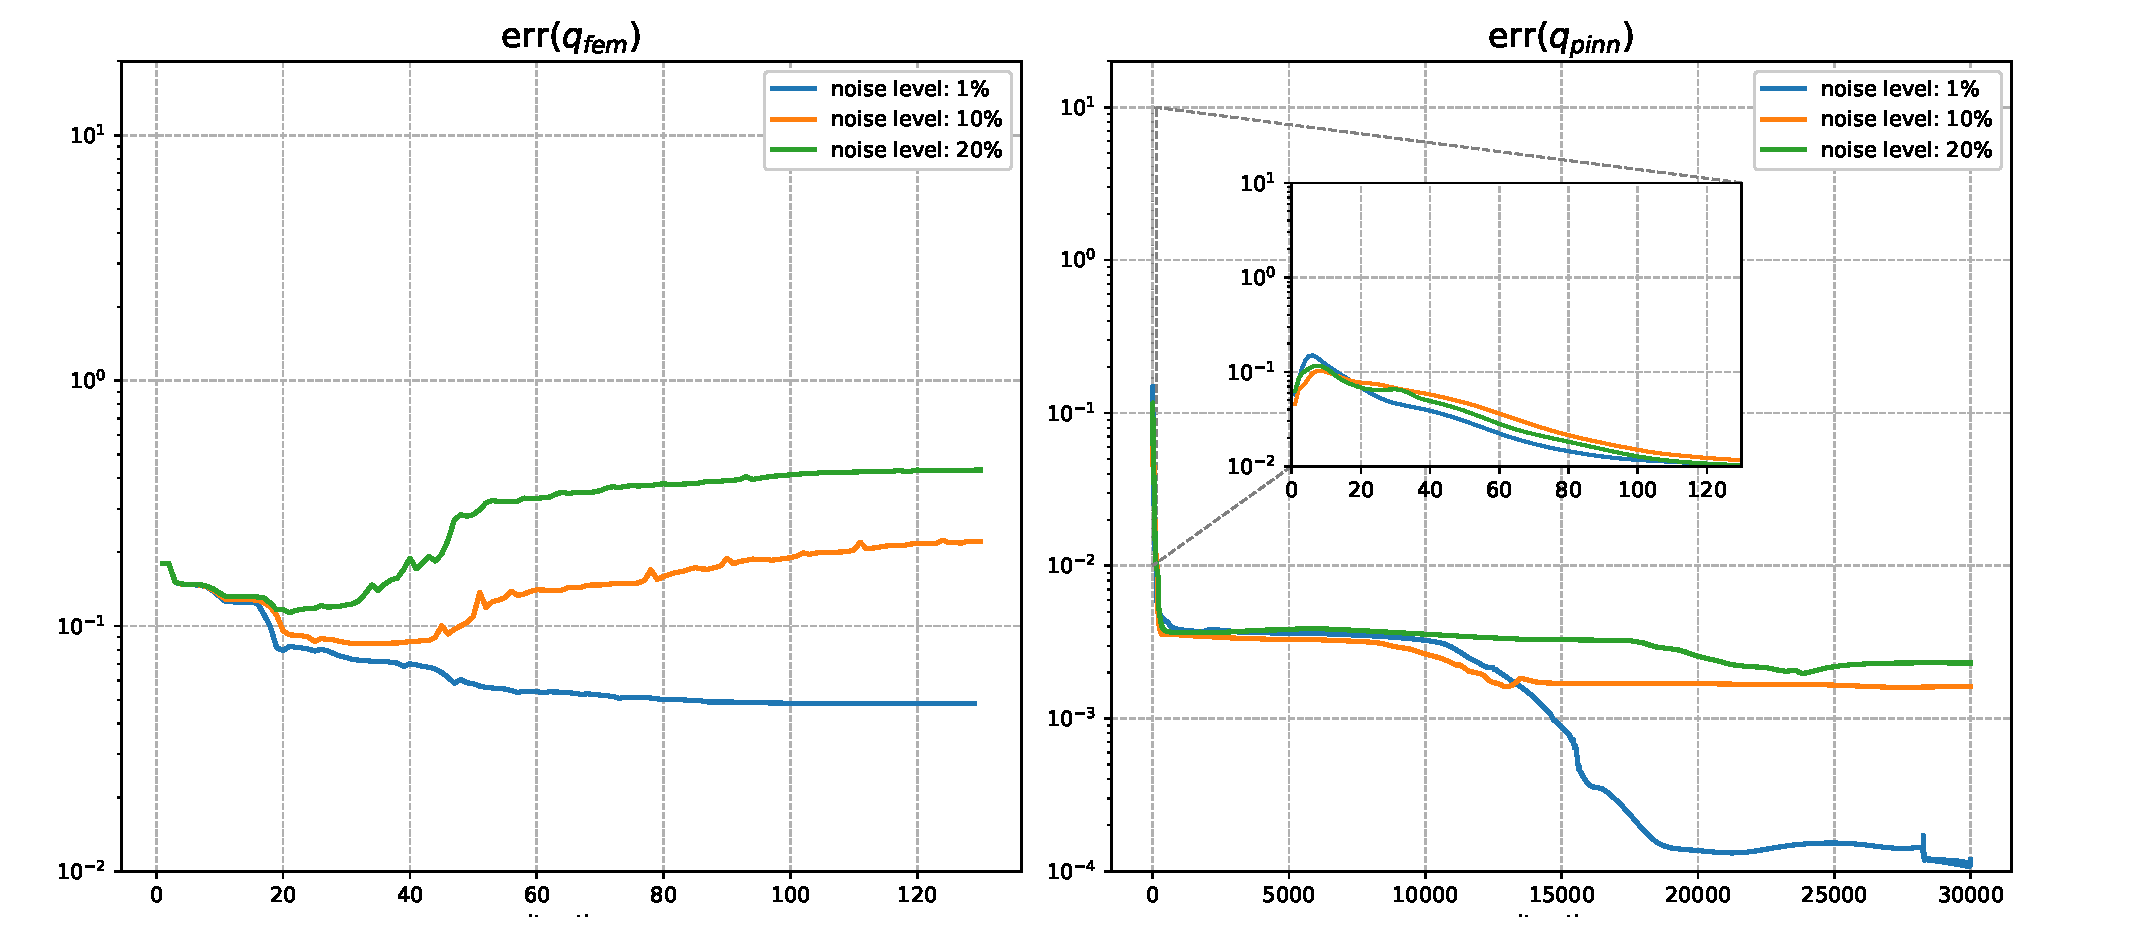
\includegraphics[width=\textwidth]{figures3/err_q.eps}
   \caption{算例~\ref{example:nonsmooth} 中重构势函数 $q$ 的相对 $L^{2}$ 误差随迭代次数变化的曲线。左列显示了有限元方法获得的结果，而右列显示了 Tikhonov-PINNs 获得的结果。}
   \label{fig:err_q}
\end{figure}

% \section{数值实验}\label{sec:numerical}

% 为验证 Tikhonov-PINNs 方法的有效性，我们进行了以下数值实验。所有实验基于 PyTorch 框架，在配备 NVIDIA Tesla V100 GPU 的服务器上完成。

% \subsection{实验设置}

% \textbf{网络结构：} 我们采用深度为 6、宽度为 100 的全连接 ReLU 网络。为保证 $H^2$ 正则性，输出层前添加 ReLU$^2$ 激活函数。

% \textbf{优化器：} 使用 Adam 优化器，初始学习率 $10^{-3}$，每 5000 步衰减为原来的 0.9，总训练步数 40000。

% \textbf{采样策略：} 区域内部采样 $n_{\calI}=10000$ 个点，边界采样 $n_{\calB}=2000$ 个点。测量数据点 $m_{\calI}=5000$，$m_{\calB}=1000$。

% \textbf{超参数：} 惩罚参数 $\mu_1=1000$，$\mu_2=200$，Tikhonov 正则化参数 $\lambda=0.01$。

% \subsection{光滑势函数重构}

% 考虑二维单位正方形区域 $\Omega=[0,1]^2$，传导系数 $\alpha\equiv 1$，源项 $f\equiv 0$，通量 $g\equiv 0$。精确势函数取为：
% \begin{equation*}
% V^\dagger(x) = 2 + \sin(2\pi x_1)\cos(2\pi x_2).
% \end{equation*}

% 图 \ref{fig:eq1_twopeak} 展示了精确势函数、重构势函数及其误差的分布。可以看出，Tikhonov-PINNs 方法能够准确捕捉势函数的光滑变化特征，最大相对误差小于 5\%。

% \begin{figure}[htbp]
%     \centering
%     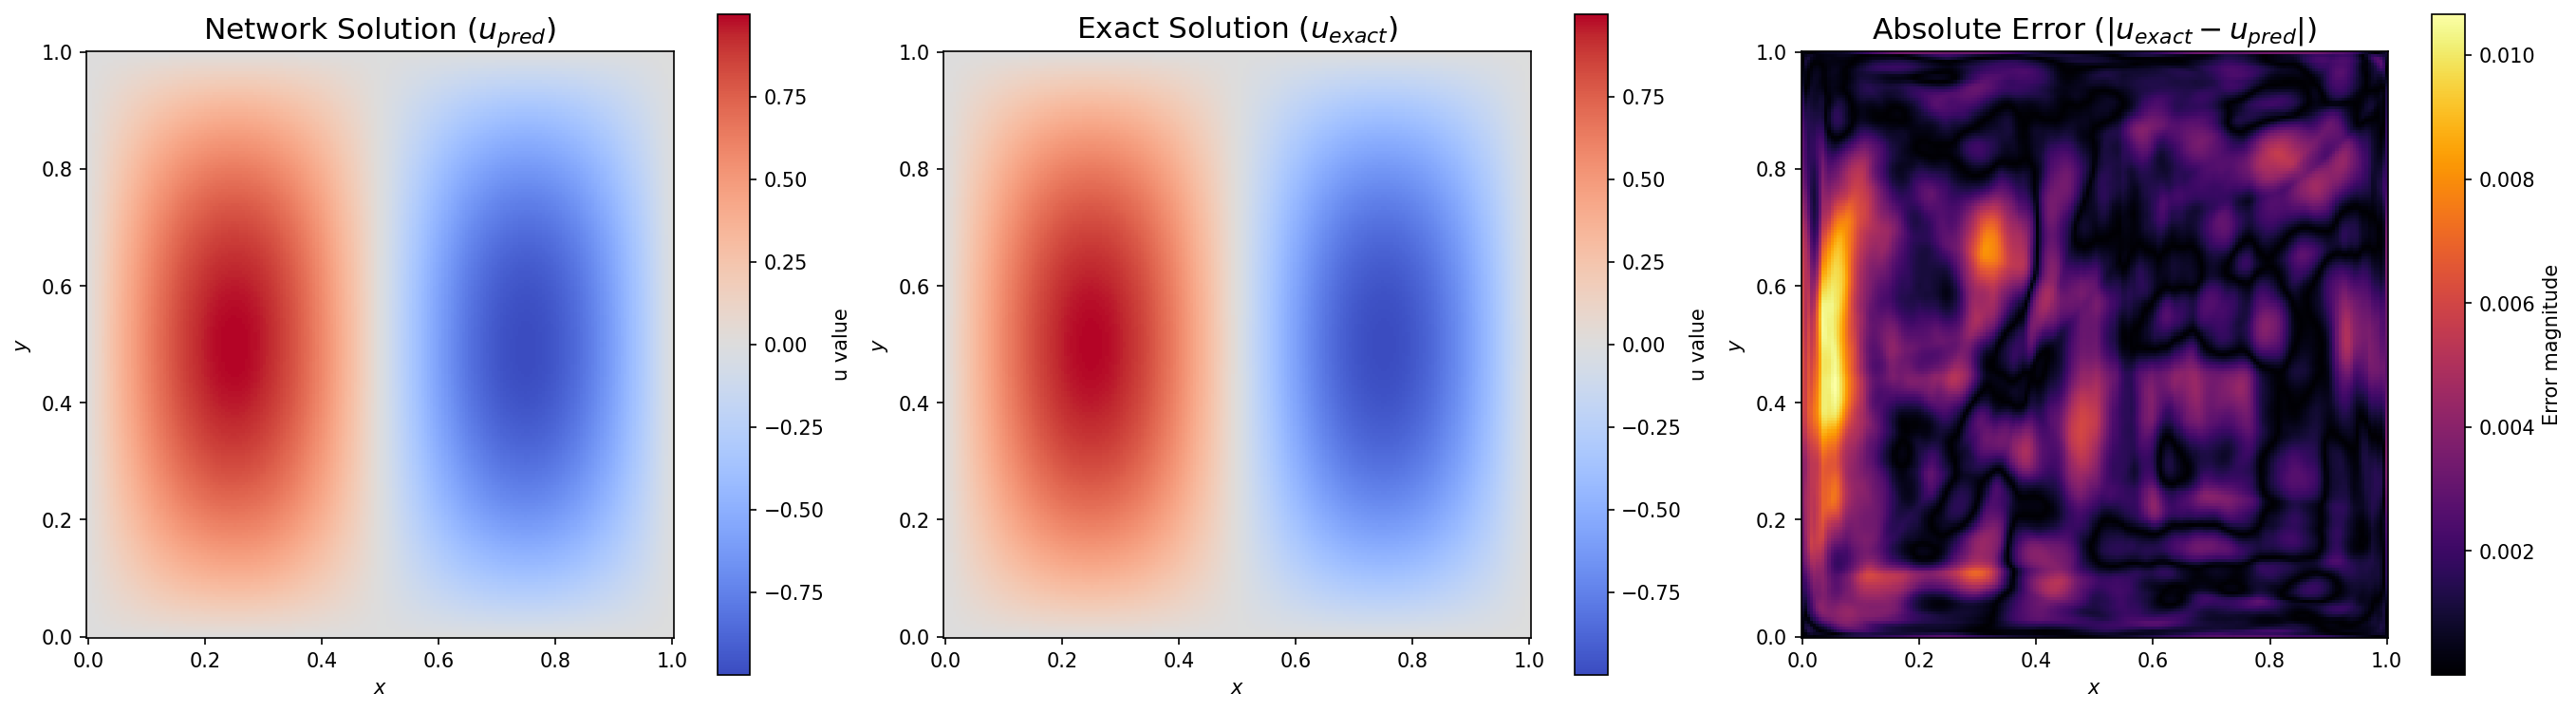
\includegraphics[width=\textwidth]{./figures2/eq1_twopeak_heatmap.png}
%     \caption{光滑势函数重构：精确解、预测解与误差分布}
%     \label{fig:eq1_twopeak}
% \end{figure}

% 图 \ref{fig:eq1_loss} 展示了训练过程中损失函数和验证误差的演化曲线。方法在约 20000 步后达到稳定收敛状态。

% \begin{figure}[htbp]
%     \centering
%     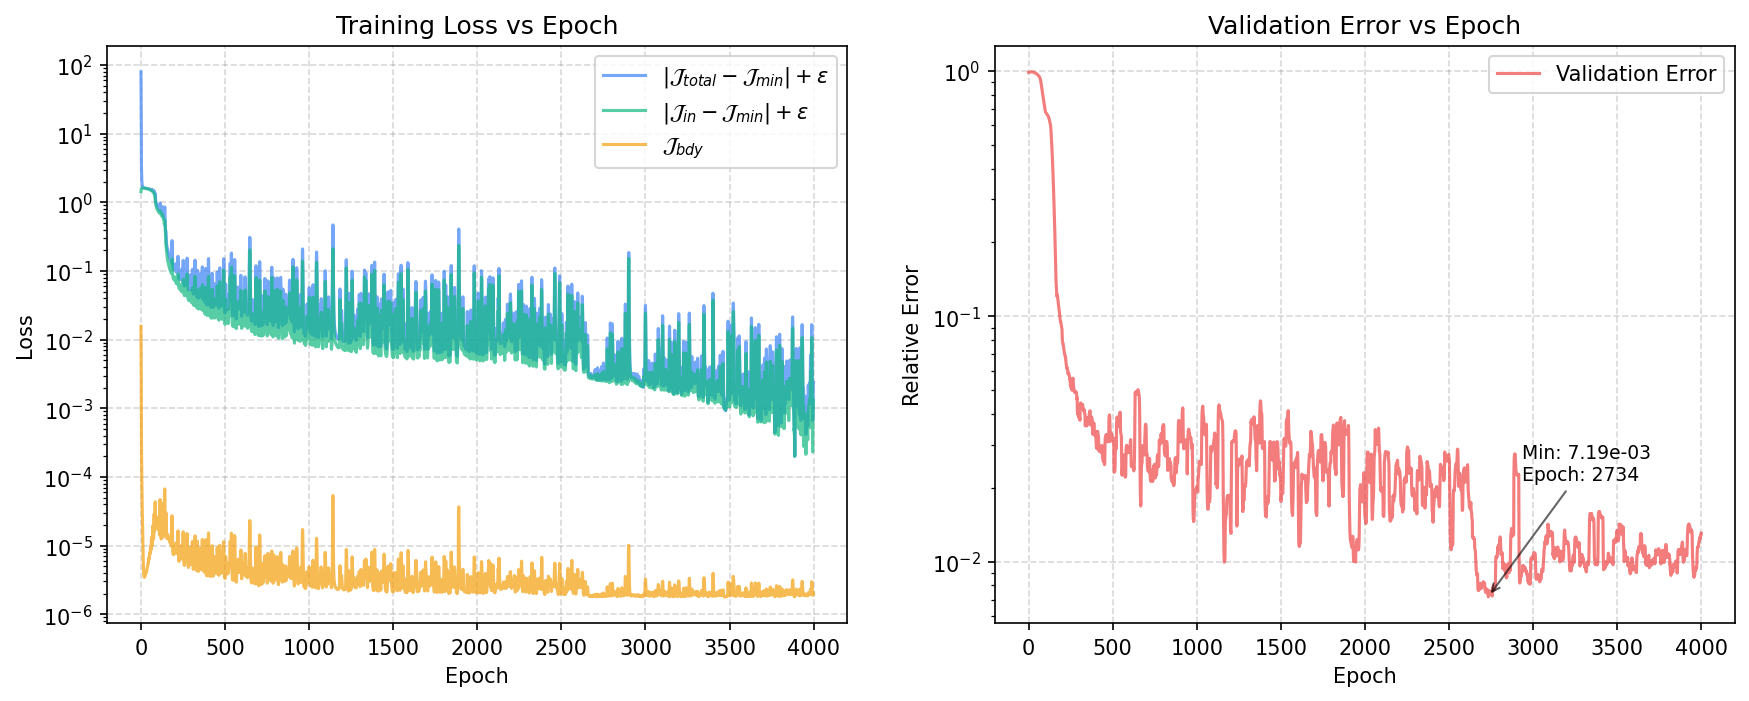
\includegraphics[width=0.9\textwidth]{./figures2/eq1_loss_val_error_curves.png}
%     \caption{光滑势函数重构：训练损失与验证误差曲线}
%     \label{fig:eq1_loss}
% \end{figure}

% \subsection{不连续势函数重构}

% 为测试方法对非光滑势函数的适应能力，考虑分段常数势函数：
% \begin{equation*}
% V^\dagger(x) = \begin{cases}
% 3, & \|x - (0.5, 0.5)\|_2 < 0.3, \\
% 1, & \text{其他}.
% \end{cases}
% \end{equation*}

% 图 \ref{fig:eq2_nondiff} 展示了重构结果。尽管势函数在间断处不可导，Tikhonov-PINNs 方法仍能较准确地捕捉势函数的整体分布，间断边界处的相对误差约为 10\%。

% \begin{figure}[htbp]
%     \centering
%     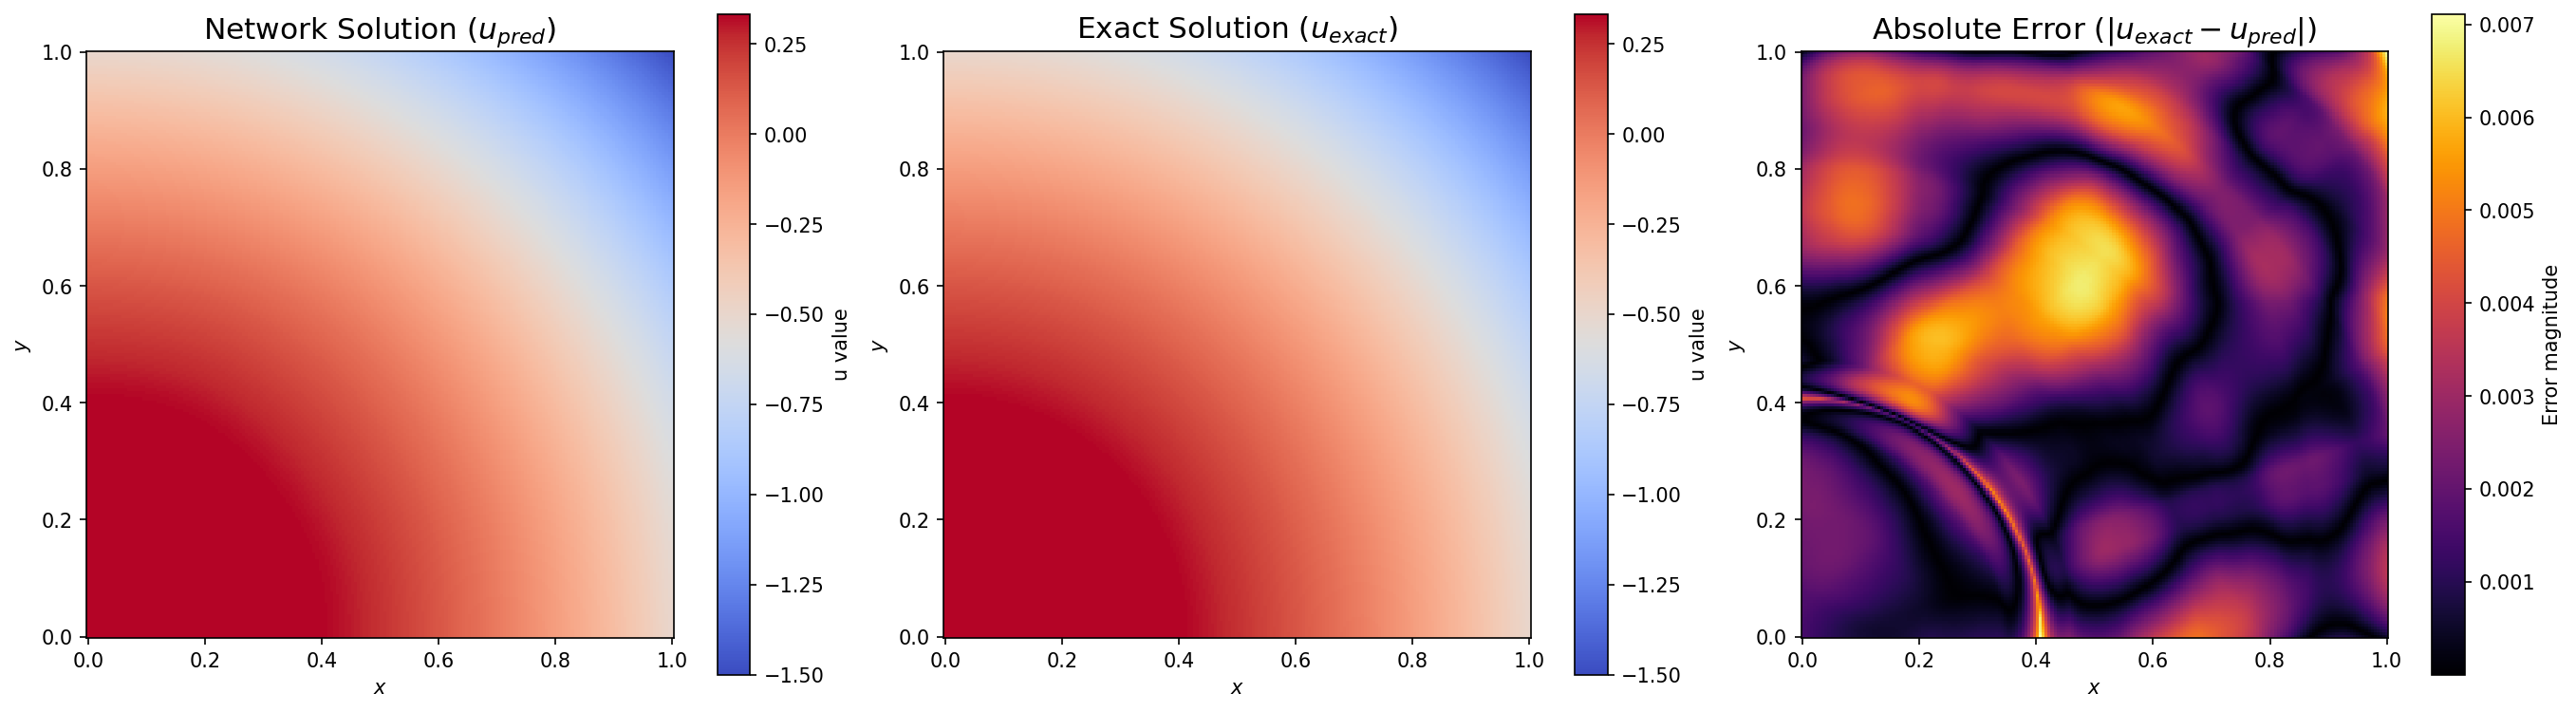
\includegraphics[width=\textwidth]{./figures2/eq2_nondiff_heatmap.png}
%     \caption{不连续势函数重构：精确解、预测解与误差分布}
%     \label{fig:eq2_nondiff}
% \end{figure}

% \subsection{不同噪声水平下的鲁棒性}

% 我们测试了方法在不同噪声水平 $\delta$ 下的表现。表 \ref{tab:noise} 列出了不同噪声水平下的相对误差。结果显示，随着噪声水平的降低，重构精度单调提高，验证了方法的鲁棒性。

% \begin{table}[htbp]
% \centering
% \caption{不同噪声水平下的重构误差}
% \label{tab:noise}
% \begin{tabular}{c|ccccc}
% \hline
% 噪声水平 $\delta$ & 0.1 & 0.05 & 0.02 & 0.01 & 0.005 \\
% \hline
% 相对误差 (\%) & 18.3 & 12.1 & 6.5 & 3.8 & 2.1 \\
% \hline
% \end{tabular}
% \end{table}


\section{附录}\label{sec:appendix}

\chapter{物理信息驱动的神经网络方法求解反势能问题}
\section{引言}
令 $\Omega\subseteq \bbR^{d}$ ($d\geq1$) 为一个具有光滑边界 $\partial\Omega$ 的有界连通区域。在本文中，我们考虑以下椭圆边值问题的势函数辨识
\begin{equation}\label{eq:pde:potential}
\left\{
\begin{aligned}
-\nabla\cdot(\alpha\nabla u)+qu&=f, \quad \text{在}~\Omega~\text{中},\\
\alpha\partial_{\nu}u&=g, \quad \text{在}~\partial\Omega~\text{上},
\end{aligned}
\right.
\end{equation}
其中给定了传导（或扩散）系数 $\alpha\in C^{1}(\bar{\Omega})$，源密度 $f\in L^{2}(\Omega)$ 和通量 $g\in L^{2}(\partial\Omega)$。空间依赖的势函数 $q$ 属于容许集
\begin{equation}\label{eq:box}
\calK=\{q\in L^{\infty}(\Omega):0\leq\underline{q}\leq q(x)\leq\overline{q}<\infty,~x\in\Omega\}.
\end{equation}
这里常数 $\underline{q}$ 和 $\overline{q}$ 分别代表容许势函数 $q(x)$ 的下界和上界。方程 \eqref{eq:pde:potential} 可以被视为与时间无关的 Schr{\"o}dinger 方程 \cite{Bal2010Inverse}，其中 $q$ 是势函数。它还描述了扩散和热传递中的现象。具体而言，在与时间无关的扩散方程 \cite{Bal2010Inverse} 中，$q$ 对应于吸收（或反应）系数，而在稳态热方程中，$q$ 代表辐射系数~\cite{Chen2020Convergence}。
\par 实际上，系统方程 \eqref{eq:pde:potential} 中的势函数 $q$ 通常是未知的，目标是从整个区域 $\Omega$ 及其边界 $\partial\Omega$ 上 $u$ 的含噪测量值中恢复它。给定 $q\in\calK$，方程 \eqref{eq:pde:potential} 存在唯一解 $u_{q}\in H^{1}(\Omega)$ \cite{evans2010partial}。我们因此可以定义一个正演算子 $\calF:q\mapsto u_{q}$。在整篇文章中，假设含噪测量数据是由以下标准高斯回归模型生成的
\begin{equation}\label{eq:measurement}
\left\{
\begin{array}{rcll}
z^{\delta}(x)&=&\calF(q^{\dagger})(x)+\varepsilon_{\calI}(x),\quad &\varepsilon_{\calI}(x)\sim N(0,\delta^{2}),\quad x\in\Omega, \\ 
Tz^{\delta}(x)&=&T\calF(q^{\dagger})(x)+\varepsilon_{\calB}(x),\quad &\varepsilon_{\calB}(x)\sim N(0,\delta^{2}),\quad x\in\partial\Omega,
\end{array}
\right.
\end{equation}
其中 $q^\dagger$ 代表真实的势函数，$\delta$ 表示正的噪声水平，$T$ 是迹算子。很容易验证 $\|z^{\delta}-\calF(q^{\dagger})\|_{L^{2}(\Omega)}=|\Omega|^{1/2}\delta$ 且 $\|Tz^{\delta}-T\calF(q^{\dagger})\|_{L^{2}(\partial\Omega)}=|\partial\Omega|^{1/2}\delta$。

在本文中，我们提出了 Tikhonov-PINNs，一种基于神经网络的求解反势问题的方法。该方法背后的核心概念是将 Tikhonov 正则化与 PINNs 相结合。与~\cite{duan2024recovering} 不同，我们像 \cite{jin2024stochastic} 中那样，为非线性势识别问题的随机收敛性建立了误差估计，将适用范围扩展到了线性场景和有界噪声考量之外。综上所述，我们的主要贡献列举如下：

\begin{itemize}
\item[(i)] 我们提出了 Tikhonov-PINNs，这是一种通过整合 Tikhonov 正则化和 PINNs 来求解反势问题的无网格数值重构算法。通过这种整合，我们为反势问题引入了新的稳定性估计，建立了物理信息损失误差与重构收敛率之间的联系。

\item[(ii)] 我们进行了一系列数值实验来展示 Tikhonov-PINNs 的有效性。通过将其应用于不同噪声水平测量下的光滑和不连续势函数，我们要证明所提出的方法在精度和鲁棒性方面均优于经典的基于有限元的方法以及原始 PINNs。

\item[(iii)] 我们给出了 Tikhonov-PINNs 的系统性收敛分析。我们的理论结果表明，在合适的神经网络参数和 $u$ 的一些正性条件下，重构解 $\hat{q}$ 表现出如下趋向于真实值 $q^{\dagger}$ 的收敛行为：
\[
\mathbb{E}_{\calS}\left[\|\hat{q}-q^\dagger\|_{L^2(\Omega)}\right] \leq \mathcal{O}\left(\delta^{\frac{1}{2(1+2\beta)}}\cdot\max\left\{ \log\left( \frac{1}{\delta} \right), 1 \right\}\right).
\]
期望 $\mathbb{E}_{\calS}$ 是在随机样本 $\calS$ 上选取的，$\beta>0$ 为常数。详情请参见定理 \ref{thm:excess} 和定理 \ref{thm:ConvergenceRate}。进一步的分析表明，我们的方法部分克服了维数灾难 (CoD)。
\end{itemize}

本文的其余部分组织如下。在第 \ref{prelim} 节中，我们介绍了预备知识和符号说明。针对反势问题的重构方法，即 Tikhonov-PINNs，随后在第 \ref{sec:tikpinns} 节中进行介绍。误差分析结果在第 \ref{sec:erroranalysis} 节中陈述，其证明包含在第 \ref{sec:proof} 节中。在第 \ref{sec:numerical} 节中，我们提供了一些数值算例以展示我们方法的有效性。最后，我们在第 \ref{sec:conclusion} 节中给出结论并进行进一步讨论。



\section{预备知识与符号说明}\label{prelim}




\section{重构方法：Tikhonov-PINNs}\label{sec:tikpinns}
\par 给定 Eq.\eqref{eq:measurement} 中的测量数据，我们利用 $H^2$ 范数惩罚项来重构 $q$：

\begin{equation*}
\min_{q\in\calK}\Big\{J_{\lambda}(q)=\|z^{\delta}-\calF(q)\|_{L^{2}(\Omega)}^{2}+\|Tz^{\delta}-T\calF(q)\|_{L^{2}(\partial\Omega)}^{2}+\lambda\|q\|_{H^{2}(\Omega)}^{2}\Big\},
\end{equation*}
这等价于一个线性二次椭圆控制问题
\begin{align*}
&\min_{q,u}\quad\calJ_{\lambda}(q,u)=\|z^{\delta}-u\|_{L^{2}(\Omega)}^{2}+\|Tz^{\delta}-Tu\|_{L^{2}(\partial\Omega)}^{2}+\lambda\|q\|_{H^{2}(\Omega)}^{2}, \\
&\subto\quad Eq.\eqref{eq:pde:potential}~\text{and}~Eq.\eqref{eq:box}.
\end{align*}
处理上述 PDE 约束优化问题的一个自然方法是引入物理信息惩罚项，将其转化为无约束问题
\begin{equation}\label{eq:pinns:loss}
\min_{q,u}\Big\{\calL_{\lambda}(q,u)=\calJ_{\lambda}(q,u)+\calI(q,u)+\calB(q,u)\Big\},
\end{equation}
其中
\begin{equation*}
\calI(q,u)=\|\nabla\cdot(\alpha\nabla u)-qu+f\|_{L^{2}(\Omega)}^{2}\quad\text{and}\quad
\calB(u)=\|\alpha\partial_{\nu}u-g\|_{L^{2}(\partial\Omega)}^{2}.
\end{equation*}
与传统 PINNs 不同，我们在损失函数中引入了一个额外的 Tikhonov 正则化项。正如我们将在下文中证明的，这一调整确保了重构势函数 $q$ 的收敛性。这在文献中通常被称为稳定性估计。为了推导这一结果，我们对 $q$ 和 $u$ 施加如下正则性假设。
\begin{assumption}\label{ass:potential:qudaggerreg}
令 $s \in \mathbb{N}_+$，我们假设 $q^\dagger \in W^{2,\infty}(\Omega) \cap H^{s+3}(\Omega) \cap K$ 且 $u^\dagger \in W^{2,\infty}(\Omega) \cap H^{s+3}(\Omega)$。
\end{assumption}
\begin{theorem}[稳定性估计]\label{th:potential:stability}
在 Eq.\eqref{eq:pde:potential} 和 Eq.\eqref{eq:measurement} 的模型下。令 $(q^{\dagger},u^{\dagger})$ 满足 Eq.\eqref{eq:pde:potential}。假设 Assumption \ref{ass:potential:qudaggerreg} 成立，则对于每一对满足 $q\in H^{2}(\Omega)$ 的 $(q,u)$，有
\begin{equation*}
\|(q-q^{\dagger})u^{\dagger}\|_{L^{2}(\Omega)}\leq C(1+\lambda^{-1/4}\calL_{\lambda}^{1/4}(q,u))(\calL_{\lambda}^{1/4}(q,u)+\delta^{1/2}),
\end{equation*}
其中 $C$ 是一个依赖于 $d$, $\Omega$, $\alpha$, $\overline{q}$, $\|q^{\dagger}\|_{W^{2,\infty}(\Omega)}$ 和 $\|u^{\dagger}\|_{W^{2,\infty}(\Omega)}$ 的正常数。
\end{theorem}
\begin{proof}
详细证明见 \ref{sec:lemma4} 小节。
\end{proof}
\par 在实际应用中，只能获得由 Eq.\eqref{eq:measurement} 生成的有限测量数据。令 $\euD_{\calI}=\{(x_{i},z_{i}^{\delta})\}_{i=1}^{m_{\calI}}$ 和 $\euD_{\calB}=\{(\bar{x}_{i},Tz_{i}^{\delta})\}_{i=1}^{m_{\calB}}$ 为测量数据集，其中 $\{x_{i}\}_{i=1}^{m_{\calI}}\subseteq\Omega$, $\{\bar{x}_{i}\}_{i=1}^{m_{\calB}}\subseteq\partial\Omega$, $z_{i}^{\delta}=z^{\delta}(x_{i})$ 且 $\bar{z}_{i}^{\delta}=Tz^{\delta}(\bar{x}_{i})$。假设 $\euX_{\calI}=\{x_{j}^{\calI}\}_{j=1}^{n_{\calI}}$ 和 $\euX_{\calB}=\{x_{j}^{\calB}\}_{j=1}^{n_{\calB}}$ 是分别从 $\Omega$ 和 $\partial\Omega$ 上的均匀分布中独立同分布抽取的两组点集。
通过将测量数据集代入目标泛函并使用蒙特卡洛方法离散化积分，我们可以获得如下经验损失函数
\begin{equation}\label{eq:empirical:loss}
\what{\calL}_{\lambda}(q,u)=\what{\calJ}_{\lambda}(q,u)+\what{\calI}(q,u)+\what{\calB}(u),
\end{equation}
该函数以数据集 $\euD_{\calI}$，$\euD_{\calB}$，$\euX_{\calI}$ 和 $\euX_{\calB}$ 为条件。其中
\begin{align*}
\what{\calJ}_{\lambda}(q,u)&=\|z^{\delta}-u\|_{L^{2}(\euD_{\calI})}^{2}+\|Tz^{\delta}-Tu\|_{L^{2}(\euD_{\calB})}^{2}+\lambda\|q\|_{H^{2}(\euX_{\calI})}^{2} \\
&=\frac{|\Omega|}{m_{\calI}}\sum_{i=1}^{m_{\calI}}(z_{i}^{\delta}-u(x_{i}))^{2}+\frac{|\partial\Omega|}{m_{\calB}}\sum_{i=1}^{m_{\calB}}(\bar{z}_{i}^{\delta}-Tu(\bar{x}_{i}))^{2} \\
&\quad+\lambda\frac{|\Omega|}{n_{\calI}}\sum_{j=1}^{n_{\calI}}\Big\{q(x_{j}^{\calI})^{2}+\sum_{k=1}^{d}\partial_{k}q(x_{j}^{\calI})^{2}+\sum_{k=1}^{d}\sum_{\ell=1}^{d}\partial_{k}\partial_{\ell}q(x_{j}^{\calI})^{2}\Big\}, \\
\what{\calI}(q,u)&=\|\nabla\cdot(\alpha\nabla u)-qu+f\|_{L^{2}(\euX_{\calI})}^{2} \\
&=\frac{|\Omega|}{n_{\calI}}\sum_{j=1}^{n_{\calI}}(\nabla\cdot(\alpha(x_{j}^{\calI})\nabla u(x_{j}^{\calI}))-q(x_{j}^{\calI})u(x_{j}^{\calI})+f(x_{j}^{\calI}))^{2}, \\
\what{\calB}(u)&=\|\alpha\partial_{\nu}u-g\|_{L^{2}(\euX_{\calB})}^{2}=\frac{|\partial\Omega|}{n_{\calB}}\sum_{i=1}^{n_{\calB}}(\alpha(x_{j}^{\calB})\partial_{\nu}u(x_{j}^{\calB})-g(x_{j}^{\calB}))^{2}.
\end{align*}
随后数值解被定义为在某些神经网络类 $\calQ\times\calU$ 上最小化 Eq.\eqref{eq:empirical:loss}
\begin{equation}\label{eq:erm}
(\hat{q},\hat{u})\in\argmin_{(q,u)\in\calQ\times\calU}\what{\calL}_{\lambda}(q,u).
\end{equation}
在统计学术语中，Eq.\eqref{eq:erm} 被视为经验风险最小化，这等价于参数空间上的一个优化问题
\begin{equation*}
(\hat{\theta}_{q},\hat{\theta}_{u})\in\argmin_{(\theta_{q},\theta_{u})\in\Theta_{q}\times\Theta_{u}}\what{\calL}_{\lambda}(q(\theta_{q}),u(\theta_{u})).
\end{equation*}
详细的重构过程如算法 \ref{alg:TikPINNs} 所示。
\par\noindent
\begin{minipage}{\textwidth}
\renewcommand*\footnoterule{}
\renewcommand{\thempfootnote}{\fnsymbol{mpfootnote}}
\begin{algorithm}[H]
\caption{Tikhonov-PINNs}
\label{alg:TikPINNs}
\begin{algorithmic}[1]
\Require 数据集 $\euD_{\calI}$, $\euD_{\calB}$, $\euX_{\calI}$ 和 $\euX_{\calB}$。
\State 构建由 $(\theta_{q},\theta_{u})$ 参数化的神经网络 $(q(\theta_{q}),u(\theta_{u}))$。
\State 初始化参数 $(\theta_{q},\theta_{u})$。
\State \textcolor{white!30!black}{\texttt{\# Tikhonov-PINNs 训练。}}
\State \textcolor{white!30!black}{\texttt{\# 通过 Tikhonov-PINNs 损失估计 $(q(\theta_{q}),u(\theta_{u}))$。}}
\For {$k=1:\texttt{epochs}$}
\State {计算由 Eq.\eqref{eq:empirical:loss} 定义的经验 Tikhonov-PINNs 损失
\begin{equation*}
\what{\calL}_{\lambda}(q(\theta_{q}),u(\theta_{u}))=\what{\calJ}_{\lambda}(q(\theta_{q}),u(\theta_{u}))+\what{\calI}(q(\theta_{q}),u(\theta_{u}))+\what{\calB}(u(\theta_{u})).
\end{equation*}}
\State {反向传播 $(g_{\theta_{q}},g_{\theta_{u}})=\nabla\what{\calL}(q(\theta_{q}),u(\theta_{u}))$。}
\State {通过 SGD 类算法更新 $(\theta_{q},\theta_{u})$：$(\theta_{q},\theta_{u})\leftarrow\operatorname{SGD}\big\{(\theta_{q},\theta_{u}),(g_{\theta_{q}},g_{\theta_{u}}),\tau\big\}$。}
\EndFor
\Ensure {$(\hat{q},\hat{u})\leftarrow(q(\theta_{q}),u(\theta_{u}))$.}
\end{algorithmic}
\end{algorithm}
\end{minipage}
\begin{remark}
通过选择合适的激活函数，可以确保 $\calQ\subseteq H^{2}(\Omega)$。因此，Eqs.\eqref{eq:pinns:loss}\eqref{eq:empirical:loss} 中的 $H^{2}$-范数惩罚项是良定的，并且在理论上是合理的。
\end{remark}



\section{误差分析}\label{sec:erroranalysis}
\par 在本节中，我们将首先对超额风险（见 Eq.\eqref{eq:excessrisk0}）进行误差分析，深度学习理论文献 \cite{Johannes2020Nonparametric,Shen2022approximation} 对此投入了大量的数学研究工作。然后，通过将超额风险的误差界与稳定性估计相结合，获得势函数重构的收敛率。为简单起见，我们假设 $\|\alpha\|_{C^{1}(\bar\Omega)}\leq B_{\alpha}$，$\|f\|_{L^{\infty}(\Omega)}\leq B_{f}$ 以及 $\|g\|_{L^{\infty}(\partial\Omega)}\leq B_{g}$。在本节以及第~\ref{sec:proof} 节的详细证明中，我们采用以下关于网络架构和样本复杂度的假设。

\begin{assumption}\label{allcondition}
令 $s\in\bbN_{+}$ 和 $\mu>0$ 为任意给定常数（在引理 \ref{lemma:app:tanh} 中引入）。我们选择如下的网络和样本复杂度：
\begin{enumerate}
\item[(i)] 令 $\varrho = \tanh$。设置 $Q = N_\varrho(L_\calQ, S_\calQ, R_\calQ)$ 和 $\mathcal{U} = N_\varrho(L_\mathcal{\calU}, S_\mathcal{\calU}, R_\mathcal{\calU})$，使得
\[
L_\calQ = c\log(d + 2), \quad S_\calQ = C \cdot \varepsilon^{-\frac{d}{s+1-\mu}}, \quad R_\calQ = C \cdot \varepsilon^{-\frac{9d+4+4\mu}{2(s+1-\mu)} - 2},
\]   
\[
L_\mathcal{\calU} = c\log(d + 2), \quad S_\mathcal{\calU} = C \cdot \varepsilon^{-\frac{d}{s+1-\mu}}, \quad R_\mathcal{\calU} = C \cdot \varepsilon^{-\frac{9d+4+4\mu}{2(s+1-\mu)} - 2}.
\]
这里 $c$ 和 $C$ 是依赖于 $s$、$\Omega$ 和 $\mu$ 的常数，而 $C$ 还依赖于 $d$。
\item[(ii)] 令 $S = \{D_I, D_B, X_I, X_B\}$ 为数据集的集合，并且数据集大小由下式给出：
\[
\mathcal{O}(m_I) = \mathcal{O}(m_B) = \mathcal{O}(n_I) = \mathcal{O}(n_B)
\]    
\[
= C\left(\|q^\dagger\|_{H^{s+3}(\Omega)}^{-2} + \|u^\dagger\|_{H^{s+3}(\Omega)}^{-2}\right) \cdot \varepsilon^{-\frac{45d+16s+32}{s+1-\mu}c\log(d+2)-2}.
\]    
\item[(iii)] 令 $(\hat{q}, \hat{u}) \in Q \times \mathcal{U}$ 为由 \eqref{eq:erm} 给出的经验风险最小化器，它依赖于 $S$。
\end{enumerate}
\end{assumption}


%Furthermore, using the definition of $(q^{\dagger},u^{\dagger})$, we get 
%\begin{equation}
%\calL_{\lambda}(q,u)\leq\|u-u^{\dagger}\|_{L^{2}(\Omega)}^{2}+\|Tu-Tu^{\dagger}\|_{L^{2}(\partial\Omega)}^{2}+\calI(q,u)+\calB(u)+\lambda\|q\|_{H^{2}(\Omega)}^{2}.
%\end{equation}
正如我们将在 \ref{sec:lemma5} 小节中展示的那样，$\calE_{\lambda}(q,u)$ 可以分解为逼近误差和泛化误差。逼近误差代表了假设类 $\mathcal{Q} \times \mathcal{U}$ 上超额风险的下确界，并刻画了该类中函数的表达能力。另一方面，泛化误差衡量了由蒙特卡洛离散化引起的差异（即总体风险与其经验对应项之间的差距）。基于神经网络的逼近理论和学习理论，我们可以证明，通过恰当地选择网络和样本复杂度，可以在这两个误差之间实现权衡，从而得出以下关于超额风险的收敛结果。

%For the As stated in Lem. \ref{lemma:approximation}, the approximation error can be made arbitrarily small, provided that functions in the hypothesis class can approximate the target functions with sufficiently small error.
%
%As shown in the proof of Lem. \ref{lemma:errdec}, the generalization error increases as the metric entropy of the hypothesis classes becomes larger and converges to zero at a rate of $\calO(1/n)$ as the number of samples $n$ increases.
%
%The approximation and generalization errors both depend on the network parameters $L$, $S$, and $R$, but exhibit opposite trends. Thus, the sample sizes should be chosen to be sufficiently large to ensure that the generalization error converges to zero. By properly choosing the hyperparameters, a trade-off between the approximation and generalization errors can be achieved, leading to the following convergence result for the excess risk.

\begin{theorem}[超额风险界]\label{thm:excess}
在模型 Eq.\eqref{eq:pde:potential} 和 Eq.\eqref{eq:measurement} 下。令 $\varepsilon \in (0, 1)$ 并记 $\delta \in (0, 1)$ 为噪声水平。假设假设 \ref{ass:potential:qudaggerreg} 成立，如果我们按照假设 \ref{allcondition} 选择网络和样本复杂度，则我们有
$$
\mathbb{E}_S[\mathcal{E}_\lambda(\hat{q}, \hat{u})] \leq C\left(\|q^\dagger\|_{H^{s+3}(\Omega)}^{2} + \|u^\dagger\|_{H^{s+3}(\Omega)}^{2}\right) \cdot \varepsilon^2 \log(\frac{1}{\varepsilon}) + C\left(\|q^\dagger\|_{H^2(\Omega)}^{2} + 1\right) \cdot \lambda.
$$
这里 $C$ 是一个依赖于 $d$, $\Omega$, $s$, $B_\alpha$, $B_f$, $B_g$, $\overline{q}$, $q^\dagger$ 和 $u^\dagger$ 的正常数。
\end{theorem}
\begin{proof}
详细证明请参见 \ref{sec:excessrisk} 小节。
\end{proof}


% \subsection{收敛率}
% 我们现在展示本文的主要定理。正如该定理所揭示的，在适当的参数选择下，随着噪声水平的降低，Tikhonov-PINNs 对 $q$ 和 $u$ 的重构误差会收敛到零。

% \begin{theorem}[Tikhonov-PINNs 的收敛率] \label{thm:ConvergenceRate}
% 在模型 Eq.\eqref{eq:pde:potential} 和 Eq.\eqref{eq:measurement} 下。令 $\delta \in (0,1)$ 为噪声水平。假定假设 \ref{ass:potential:qudaggerreg} 成立，如果我们选择 $\varepsilon = O(\delta)$, $\lambda = O(\delta^2)$ 并按照假设 \ref{allcondition} 选择网络和样本复杂度，那么我们有

% \begin{align*}
% \max\left\{ \mathbb{E}_\calS \left\lVert \hat{u}-u^{\dagger} \right\rVert_{L^{2}(\Omega)}, \mathbb{E}_\calS \left\lVert T\hat{u}-Tu^{\dagger} \right\rVert_{L^{2}(\partial\Omega)} \right\} &\leq C \cdot \delta \cdot\max\left\{ \log\left( \frac{1}{\delta} \right), 1 \right\},\\
% \mathbb{E}_\calS \left\lVert (\hat{q}-q^{\dagger})u^{\dagger} \right\rVert_{L^{2}(\Omega)} &\leq C \cdot \delta^{1/2} \cdot\max\left\{ \log\left( \frac{1}{\delta} \right), 1 \right\}.
% \end{align*}
% 此外，如果存在某个 $\beta \geq 0$ 和 $\zeta > 0$ 使得 $u^{\dagger}(x) \geq \zeta \text{ dist}(x,\partial\Omega)^{\beta}$ 在 $\Omega$ 中几乎处处成立，则
% \[
% \mathbb{E}_\calS \left\lVert \hat{q}-q^{\dagger} \right\rVert_{L^{2}(\Omega)} \leq C' \cdot \delta^{\frac{1}{2(1 + 2\beta)}} \cdot\max\left\{ \log\left( \frac{1}{\delta} \right), 1 \right\}.
% \]
% 这里 $C,C'$ 是依赖于 $d$, $\Omega$, $s$, $B_{\alpha}$, $B_{f}$, $B_{g}$, $\overline{q}$, $q^{\dagger}$, $u^{\dagger}$ 的正常数，且 $C'$ 还依赖于 $\zeta$。
% \end{theorem}

% \begin{proof}
% 这是一个结合了稳定性估计（定理 \ref{th:potential:stability}）和超额风险界（定理 \ref{thm:excess}）的直接结果。详细证明请参见 \ref{sec:convergence} 小节。
% \end{proof}

% \begin{remark}[正性条件]
%       正性条件 $u^{\dagger}(x) \geq \zeta \text{ dist}(x,\partial\Omega)^{\beta}$ 量化了解 $u^{\dagger}$ 当 $\text{dist}(x,\partial\Omega) \to 0^{+}$ 时趋于零的衰减率。
% \end{remark}

% \begin{remark}[超参数选择]
% 根据定理 \ref{thm:ConvergenceRate}，通过按照假设 4.1 中概述的方式选择神经网络和样本复杂度，可以很好地控制重构误差。然而在实际应用中，优化误差和当前分析的非最优性质可能导致基于假设 4.1 直接计算参数变得不切实际。尽管如此，如下所示，增加网络宽度和样本量可以降低重构误差。
% \end{remark}

% \begin{remark}[缓解维数灾难]
% 值得注意的是，样本集的大小和神经网络的规模都以 $O(\delta^{-cd/s})$ 的速率增加，其中 $c > 0$ 为绝对常数。这意味着如果真实值 $(q^{\dagger},u^{\dagger})$ 具有足够的平滑度，维数灾难可以得到缓解。
% \end{remark}


% \section{数值实验}\label{sec:numerical}
% 在本节中，我们提供了几个例子来说明 Tikhonov-PINNs 的效率。首先，我们概述数值设置如下。

% \subsection{实验设置}
% 在训练 Tikhonov-PINNs 时，我们分别采用两个神经网络来逼近未知解 $u$ 和势函数 $q$。每个网络都是具有 $tanh$ 激活函数和每两层之间存在残差连接的 DNN。对于所有算例，我们进行了多次运行以确保结果的可靠性，并且为每种情况提供了详细的训练设置。

% 在接下来的小节中，我们将本文提出的方法与传统的基于有限元的方法进行了比较。具体而言，我们使用了开源库 \textbf{dolfin-adjoint} \cite{mitusch2019dolfin}，该库基于 \textbf{FEniCS} \cite{alnaes2015fenics,grossmann2024can} 构建，专为求解反问题和最优控制问题而设计。该库获得了 2015 年威尔金森数值软件奖 (Wilkinson Prize for Numerical Software)，并在科学界获得了广泛的认可和采用。

% 所有数值实验均在武汉大学超算集群上进行，使用 Python 3.12.3 实现。该超算系统配备了 128GB ECC 2400MHz DDR4 内存、Intel Xeon E5-2640v4 2.4GHz CPU 和 NVIDIA Tesla V100 16GB GPU。

% 我们已在 GitHub 上发布了所有训练代码，网址为 \url{https://github.com/shiki442/Tikhonov-PINNs}。该仓库包含完整的数据生成、训练和评估流程，以及每个算例的参考配置文件，以便于读者复现和进一步探索。

% \subsection{评估}
% 为了衡量重构势函数 $\hat{q}$ 和解 $\hat{u}$ 的精度，我们采用如下定义的相对 $L^{2}$ 误差：
% \begin{equation*}
% \err(\hat{q})=\frac{\|\hat{q}-q^{\dagger}\|_{L^{2}(\Omega)}}{\|q^{\dagger}\|_{L^{2}(\Omega)}}\quad\text{and}\quad\err(\hat{u})=\frac{\|\hat{u}-u^{\dagger}\|_{L^{2}(\Omega)}}{\|u^{\dagger}\|_{L^{2}(\Omega)}},
% \end{equation*}
% 这里，$L^2$ 范数是基于网格点上的值进行近似的，即 $\|v\|_{L^{2}(\Omega)}\approx\sqrt{\frac{1}{N}\sum_{i=1}^{N}v(x_{i})^{2}}$，其中 $\{x_{i}\}_{i=1}^{N}$ 为网格点。

% \subsection{光滑势问题}

% 在本小节中，我们利用光滑算例进行定量分析。为了最小化优化误差的影响，我们使用充足的样本数量将网络训练了足够长的时间。

% \subsubsection{一维问题}
% \begin{figure}[htbp]
%     \centering
%     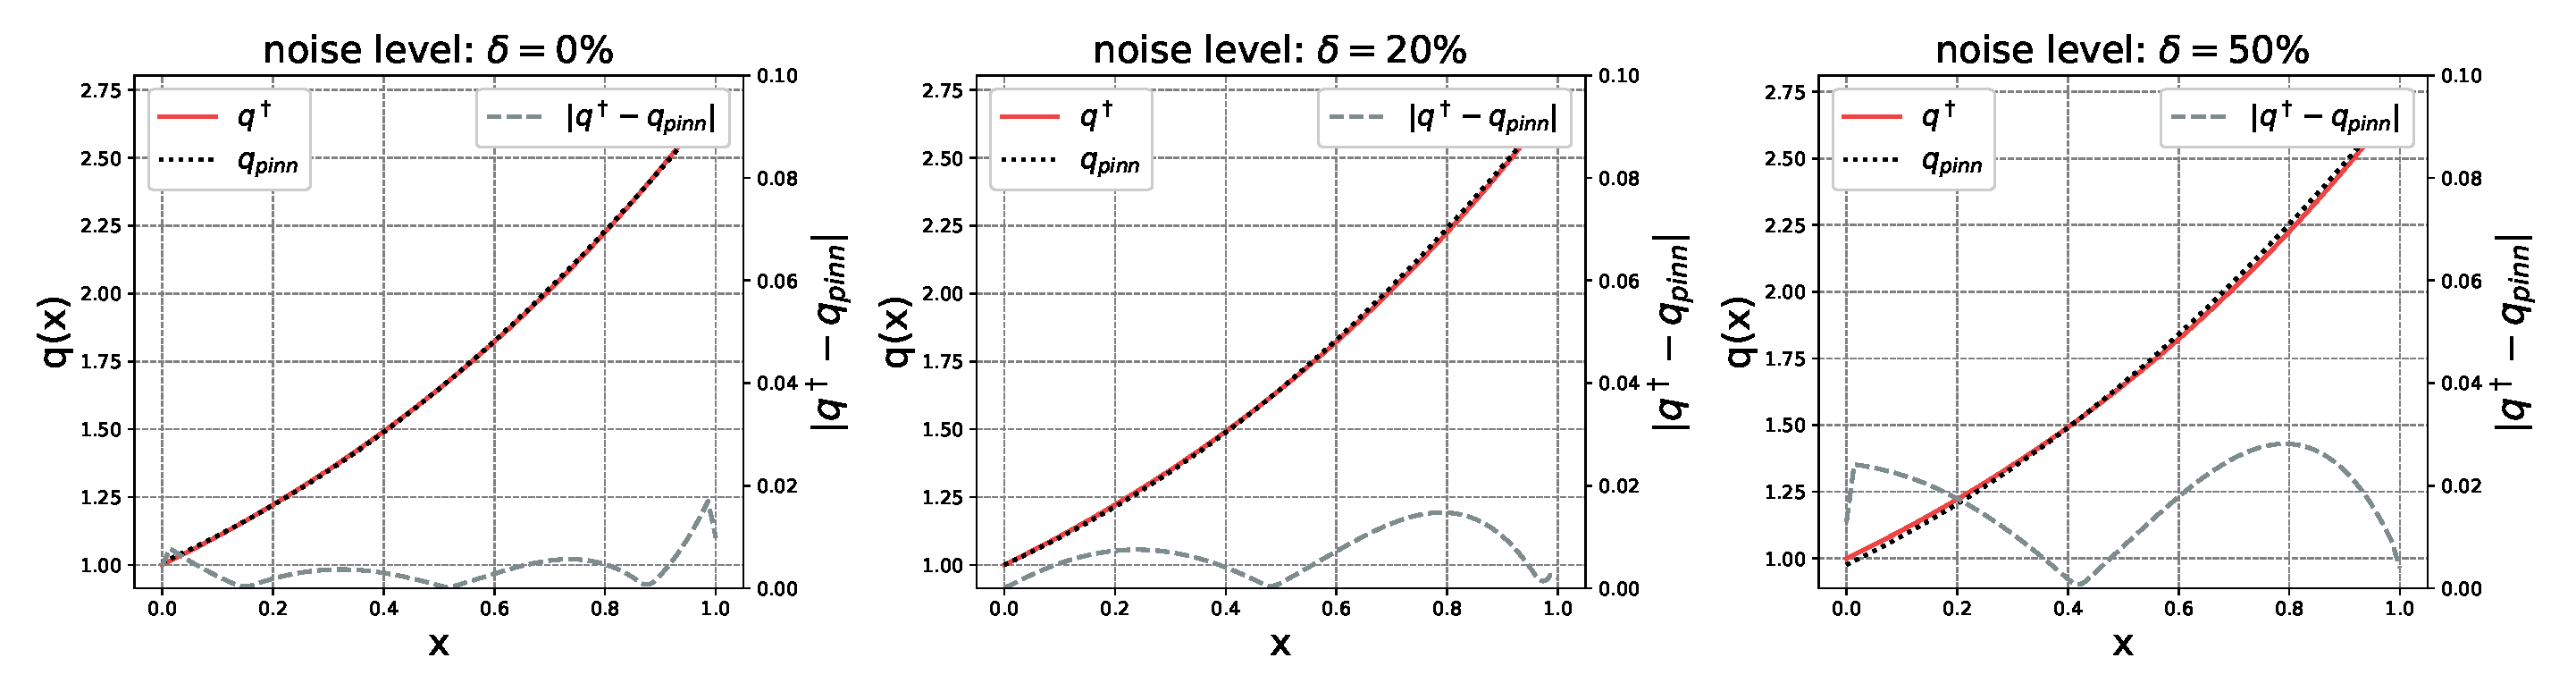
\includegraphics[width=\textwidth]{figures3/ex0_q.eps}
%     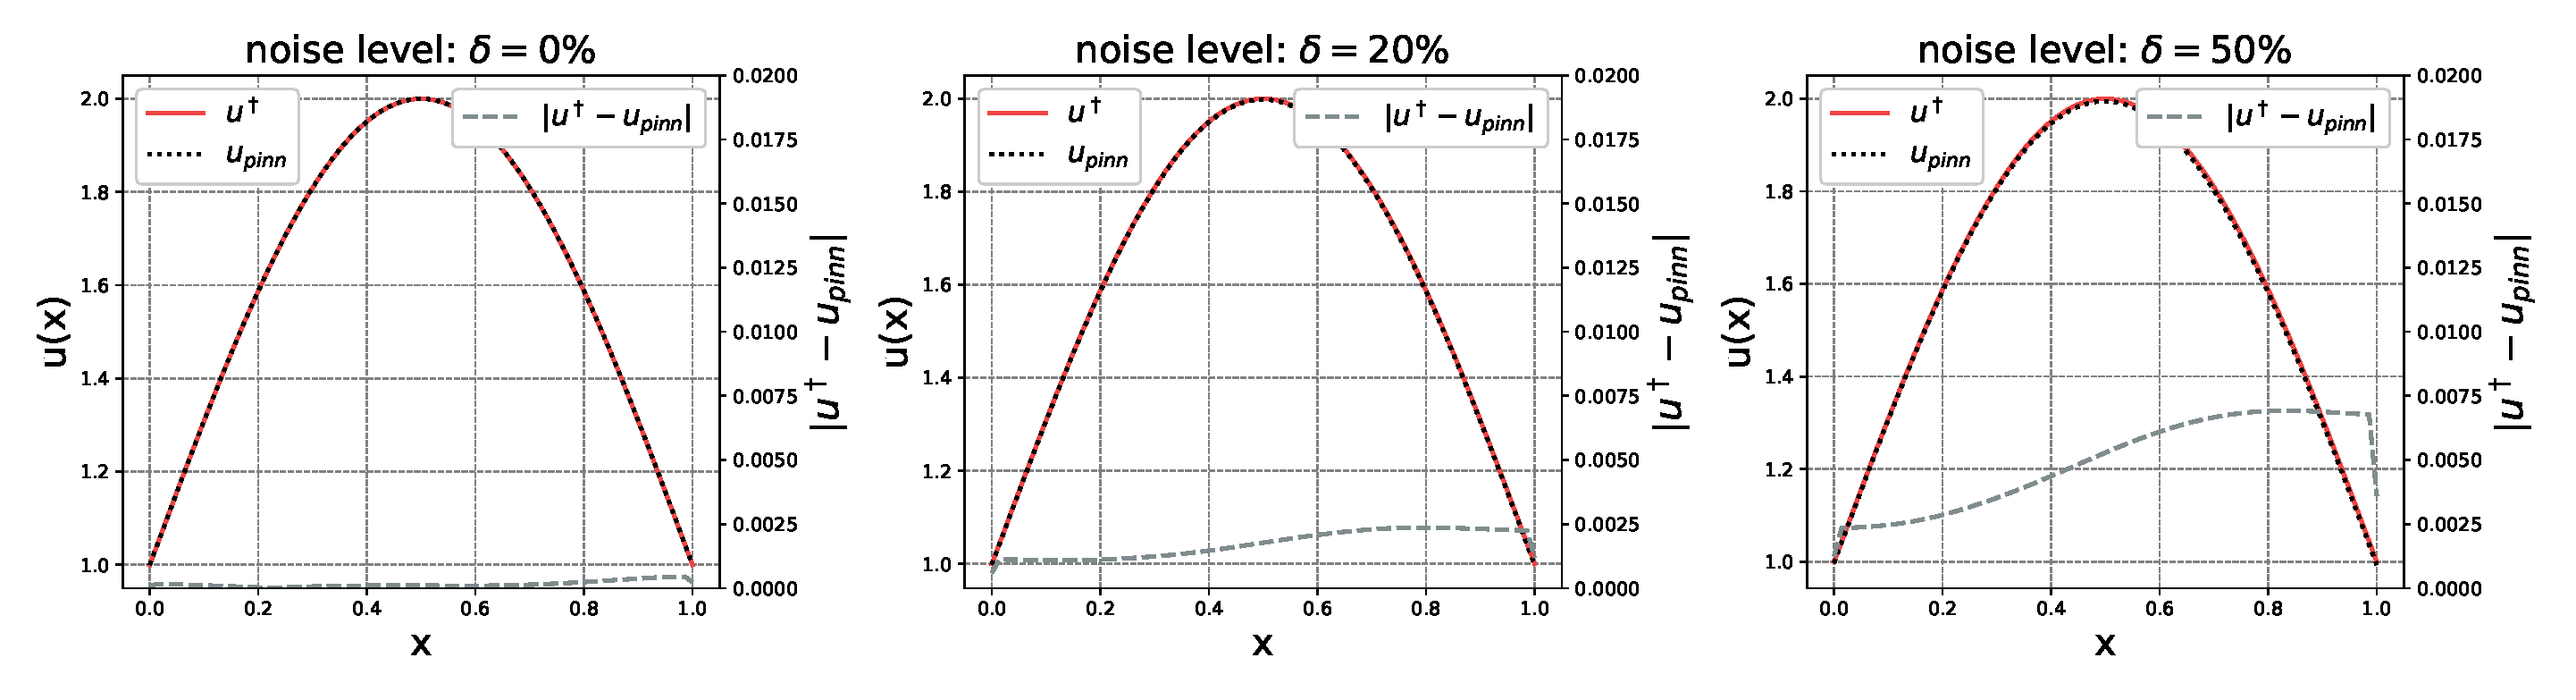
\includegraphics[width=\textwidth]{figures3/ex0_u.eps}
%     \caption{例 \ref{example:1d} 的精确解、Tikhonov-PINN 解和绝对误差。第一行对应源项 $q$，第二行对应解 $u$。从左到右，结果是在不同的噪声水平下获得的。}
%     \label{fig:ex0_q_u}
% \end{figure}

% 在本小节中，我们使用一个一维例子来验证 Tikhonov-PINNs 的收敛率，并研究超参数对重构误差的影响。
% \begin{example}\label{example:1d}
% 令 $\Omega=(0,1)$ 且 $\alpha\equiv 1$，定义精确势函数为 $q^{\dagger}(x)=\exp(x)$，对应的解为 $u^{\dagger}(x) = 1+\sin(\pi x)$。源项 $f$ 和边界条件 $g$ 由模型方程 Eq.\eqref{eq:pde:potential} 确定。
% \end{example}

% $q$ 和 $u$ 的精确解与 Tikhonov-PINNs 解如图 \ref{fig:ex0_q_u} 所示。在本例中，我们设置 $\lambda=10^{-7}$，采样 50,000 个内部点，并将边界点设为 \{0, 1\}。优化使用 Adam 优化器进行，学习率为 $10^{-4}$，迭代次数为 10,000 次。我们采用一个具有 $tanh$ 激活函数且宽度为 64 的两层神经网络来逼近 $q$ 和 $u$，并在架构中每两个相邻隐藏层之间应用残差连接。除非另有说明，本小节中的所有一维算例均使用与本例相同的默认参数设置。

% \subsubsection{收敛率}
% 在定理 \ref{thm:ConvergenceRate} 中，我们建立了 $q$ 和 $u$ 关于噪声水平 $\delta$ 的收敛率。为了验证这一结果，我们计算了不同噪声水平下 $q$ 和 $u$ 的相对误差，结果如图 \ref{fig:ex0:noise} 所示。

% \begin{figure}[htbp]
%     \centering
%     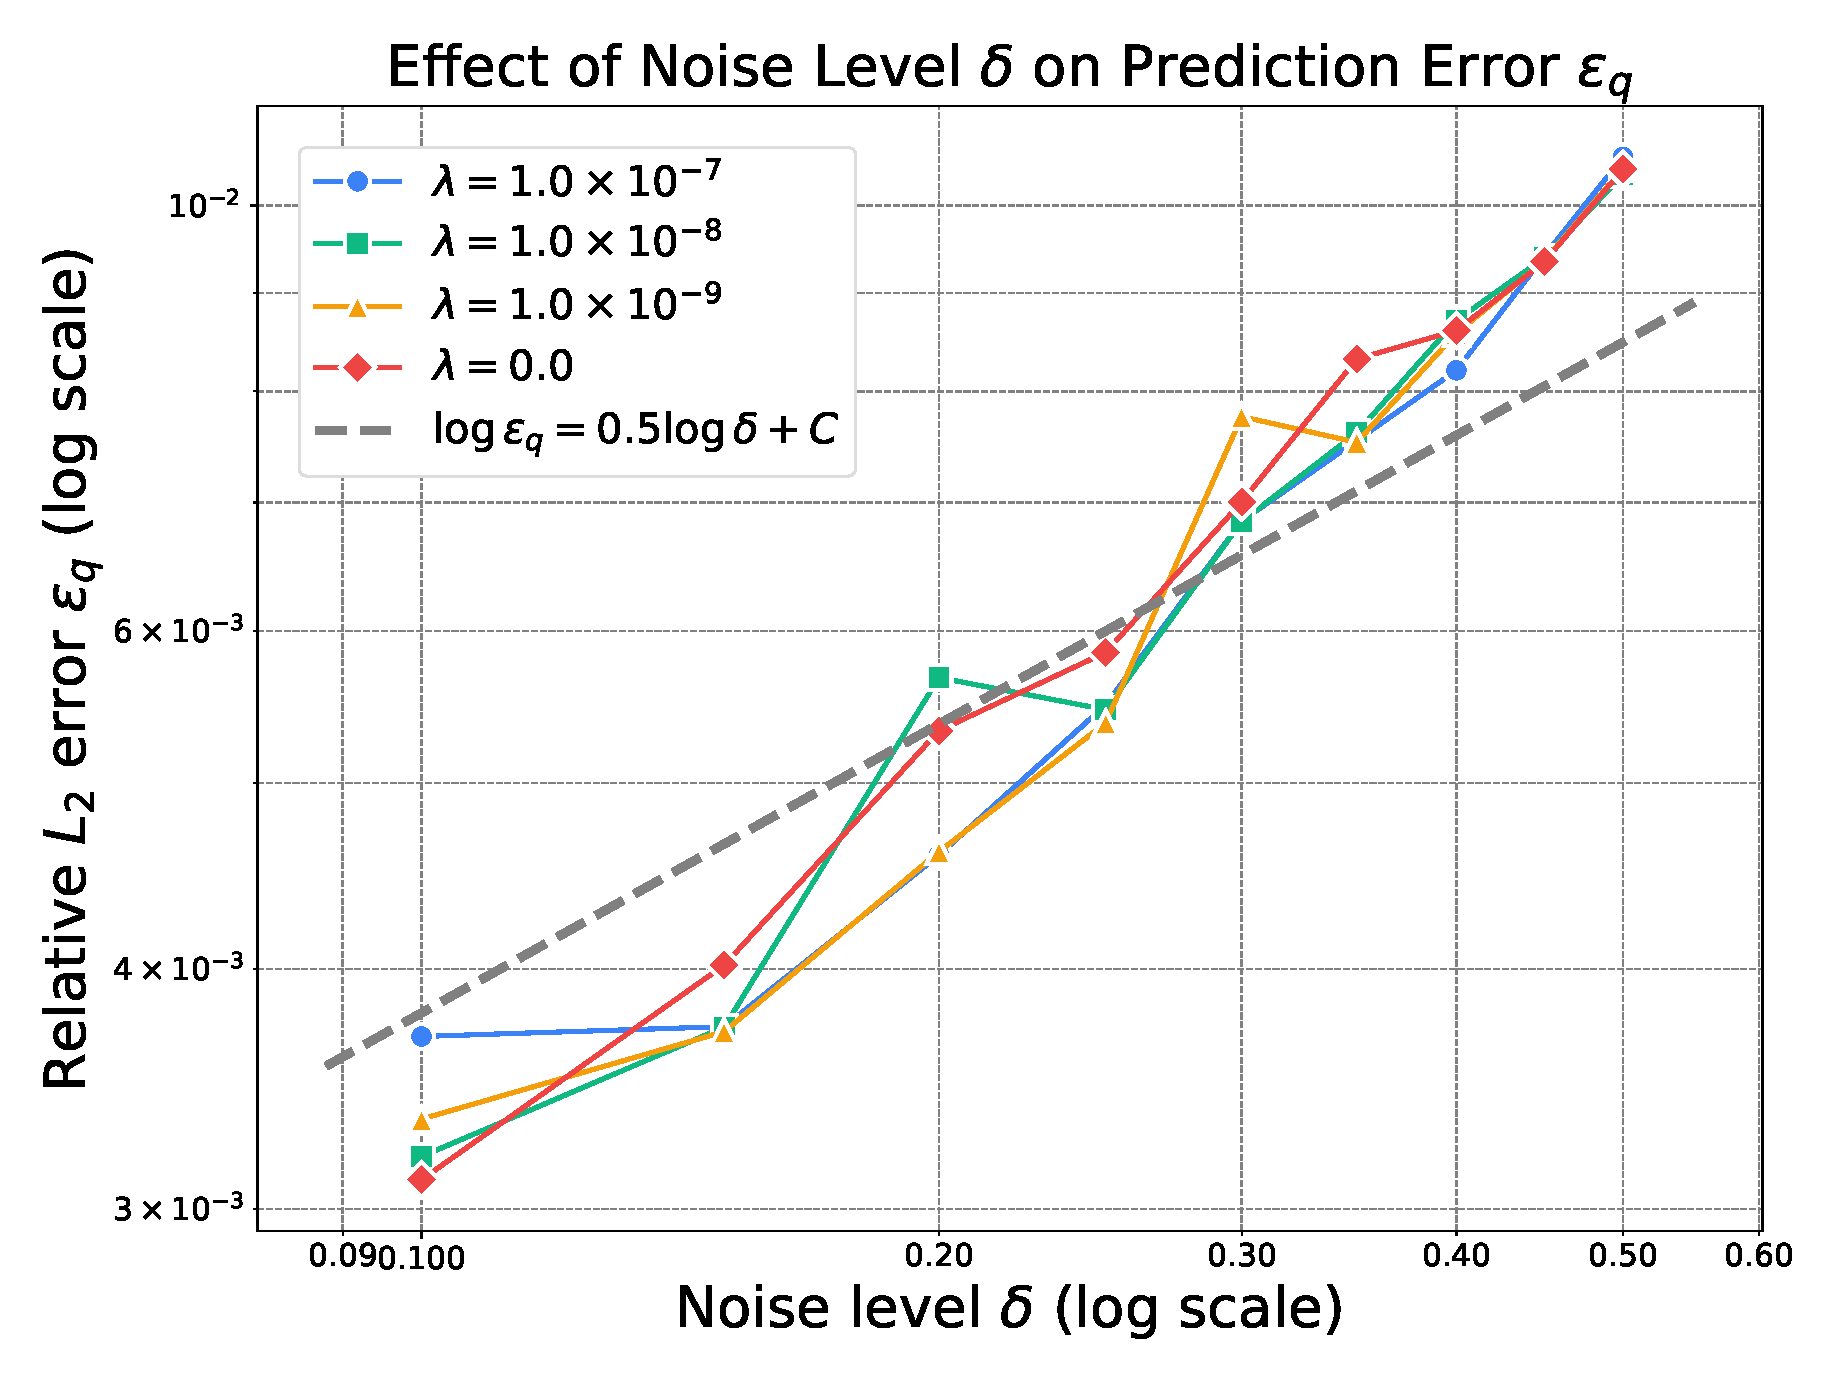
\includegraphics[width=0.49\textwidth]{figures3/ex0_noise_q.eps}
%     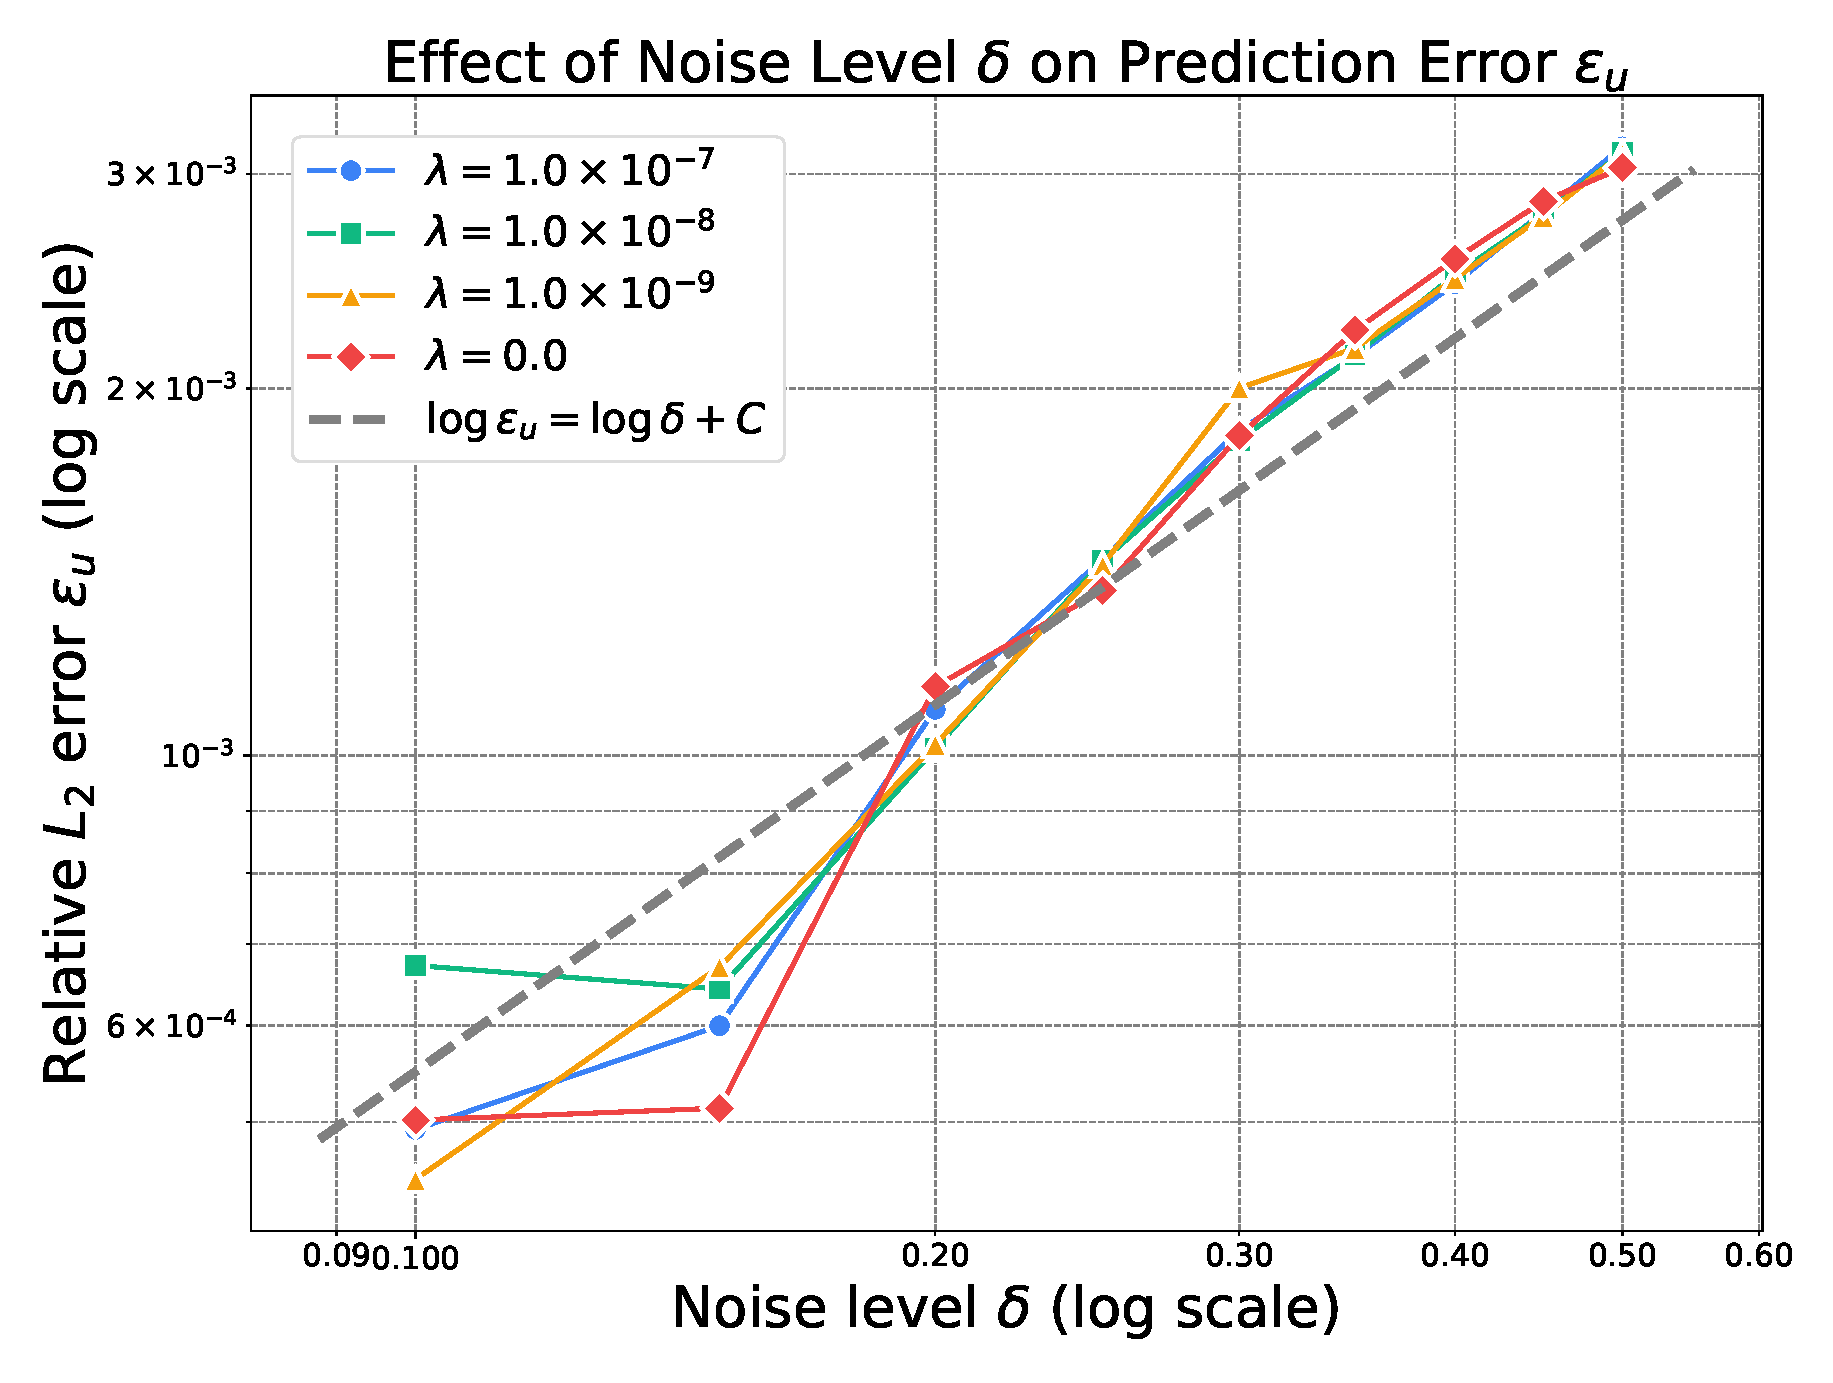
\includegraphics[width=0.49\textwidth]{figures3/ex0_noise_u.eps}
%     \caption{不同正则化参数下噪声水平对解误差的影响。左图显示了 $q$ 的结果，其中 $\lambda=$$10^{-7}$, $10^{-8}$, $10^{-9}$ 和 0 对应的对数回归曲线的斜率分别为 0.708、0.748、0.760 和 0.743，平均斜率为 0.744。右图显示了 $u$ 的结果，其中对应的斜率分别为 1.22、1.08、1.25 和 1.26，平均斜率为 1.21。}
%     \label{fig:ex0:noise}
% \end{figure}

% 由于目标势函数具有正下界，该算例满足 $\beta = 0$ 的正性条件。根据定理~\ref{thm:ConvergenceRate} 和注 \ref{compare_Gar}，$q$ 和 $u$ 的收敛率可以任意接近 $O(\delta^{0.5})$ 和 $O(\delta)$。这一点在图 \ref{fig:ex0:noise} 中得到了检验，其中 $u$ 和 $q$ 的数值收敛率与理论收敛率非常一致。平均而言，在不同的 $\lambda$ 值下，我们观察到 $u$ 的经验收敛率为 $O(\delta^{1.21})$，$q$ 的经验收敛率为 $O(\delta^{0.74})$，这实际上快于理论收敛率，表明我们的理论界可能不是最优的。

% \subsubsection{正则化的影响}
% 在本小节中，我们要研究不同正则化在求解算例 \ref{example:1d} 时的影响。如表 \ref{tab:regularization} 所示，当训练样本量相对较小（表 1 中的第一个子表）时，与 $L^2$ 正则化或原始 PINNs 相比，$H^2$ 正则化显著降低了 $q$ 的相对误差，尤其是当正则化系数 $\lambda$ 相对较大时。第二个子表表明，随着更多训练样本的可用，这种改进变得不那么明显。这是符合预期的，因为适当的正则化和增加数据量都有助于防止过拟合并提高精度。尽管如此，在两种情况下，当 $\lambda$ 选择得当时，$H^2$ 正则化都能产生最小的重构误差。这些结果凸显了 $H^2$ 正则化在求解此类反势问题时的有效性和优越性。

% \begin{table}[hbtp]
% \centering
% \footnotesize
% \caption{算例 \ref{example:1d} 中不同正则化下 $\hat{q}$ 的相对 $L^{2}$ 误差。}
% \begin{tabular}{lrrrrr}
% \hline
% \multirow{2}[0]{*}{$\text{err}(q_{\text{pinn}})$} & \multicolumn{5}{c}{正则化参数 $\lambda$} \\
% \cline{2-6}
% & \multicolumn{1}{l}{$1.0\times 10^{-3}$} & 
% \multicolumn{1}{l}{$1.0\times 10^{-4}$} &
% \multicolumn{1}{l}{$1.0\times 10^{-5}$} &
% \multicolumn{1}{l}{$1.0\times 10^{-6}$} & 
% \multicolumn{1}{l}{$1.0\times 10^{-7}$} \\
%    \hline
% $H^2$ 正则化 & $5.44\times 10^{-2}$ & $\textbf{5.26}\times \textbf{10}^{-2}$ & $8.27\times 10^{-2}$ & $8.99\times 10^{-2}$ & $9.07\times 10^{-2}$ \\
% $L^2$ 正则化 & $9.35\times 10^{-2}$ & $9.11\times 10^{-2}$ & $9.08\times 10^{-2}$ & $9.08\times 10^{-2}$ & $9.08\times 10^{-2}$ \\
% 无正则化 & $9.08\times 10^{-2}$ & $9.08\times 10^{-2}$ & $9.08\times 10^{-2}$ & $9.08\times 10^{-2}$ & $9.08\times 10^{-2}$  \\
% \hline
% &       &       &       &       & \\
% \hline
% \multirow{2}[0]{*}{$\text{err}(q_{\text{pinn}})$} & \multicolumn{5}{c}{正则化参数 $\lambda$} \\
% \cline{2-6}
% & \multicolumn{1}{l}{$1.0\times 10^{-3}$} & 
% \multicolumn{1}{l}{$1.0\times 10^{-4}$} &
% \multicolumn{1}{l}{$1.0\times 10^{-5}$} &
% \multicolumn{1}{l}{$1.0\times 10^{-6}$} & 
% \multicolumn{1}{l}{$1.0\times 10^{-7}$} \\
% \hline
% $H^2$ 正则化 & $8.96\times 10^{-2}$ & $3.14\times 10^{-2}$ & $\textbf{2.94}\times \textbf{10}^{-2}$ & $3.03\times 10^{-2}$ & $3.04\times 10^{-2}$  \\
% $L^2$ 正则化 & $3.80\times 10^{-2}$ & $3.10\times 10^{-2}$ & $3.05\times 10^{-2}$ & $3.04\times 10^{-2}$ & $3.04\times 10^{-2}$ \\
% 无正则化 & $3.04\times 10^{-1}$ & $3.04\times 10^{-2}$ & $3.04\times 10^{-2}$ & $3.04\times 10^{-2}$ & $3.04\times 10^{-2}$ \\
% \hline

% \end{tabular}
% \label{tab:regularization}
% \end{table}

% \subsubsection{其他超参数的影响}

% \begin{figure}[htbp]
%     \centering
%     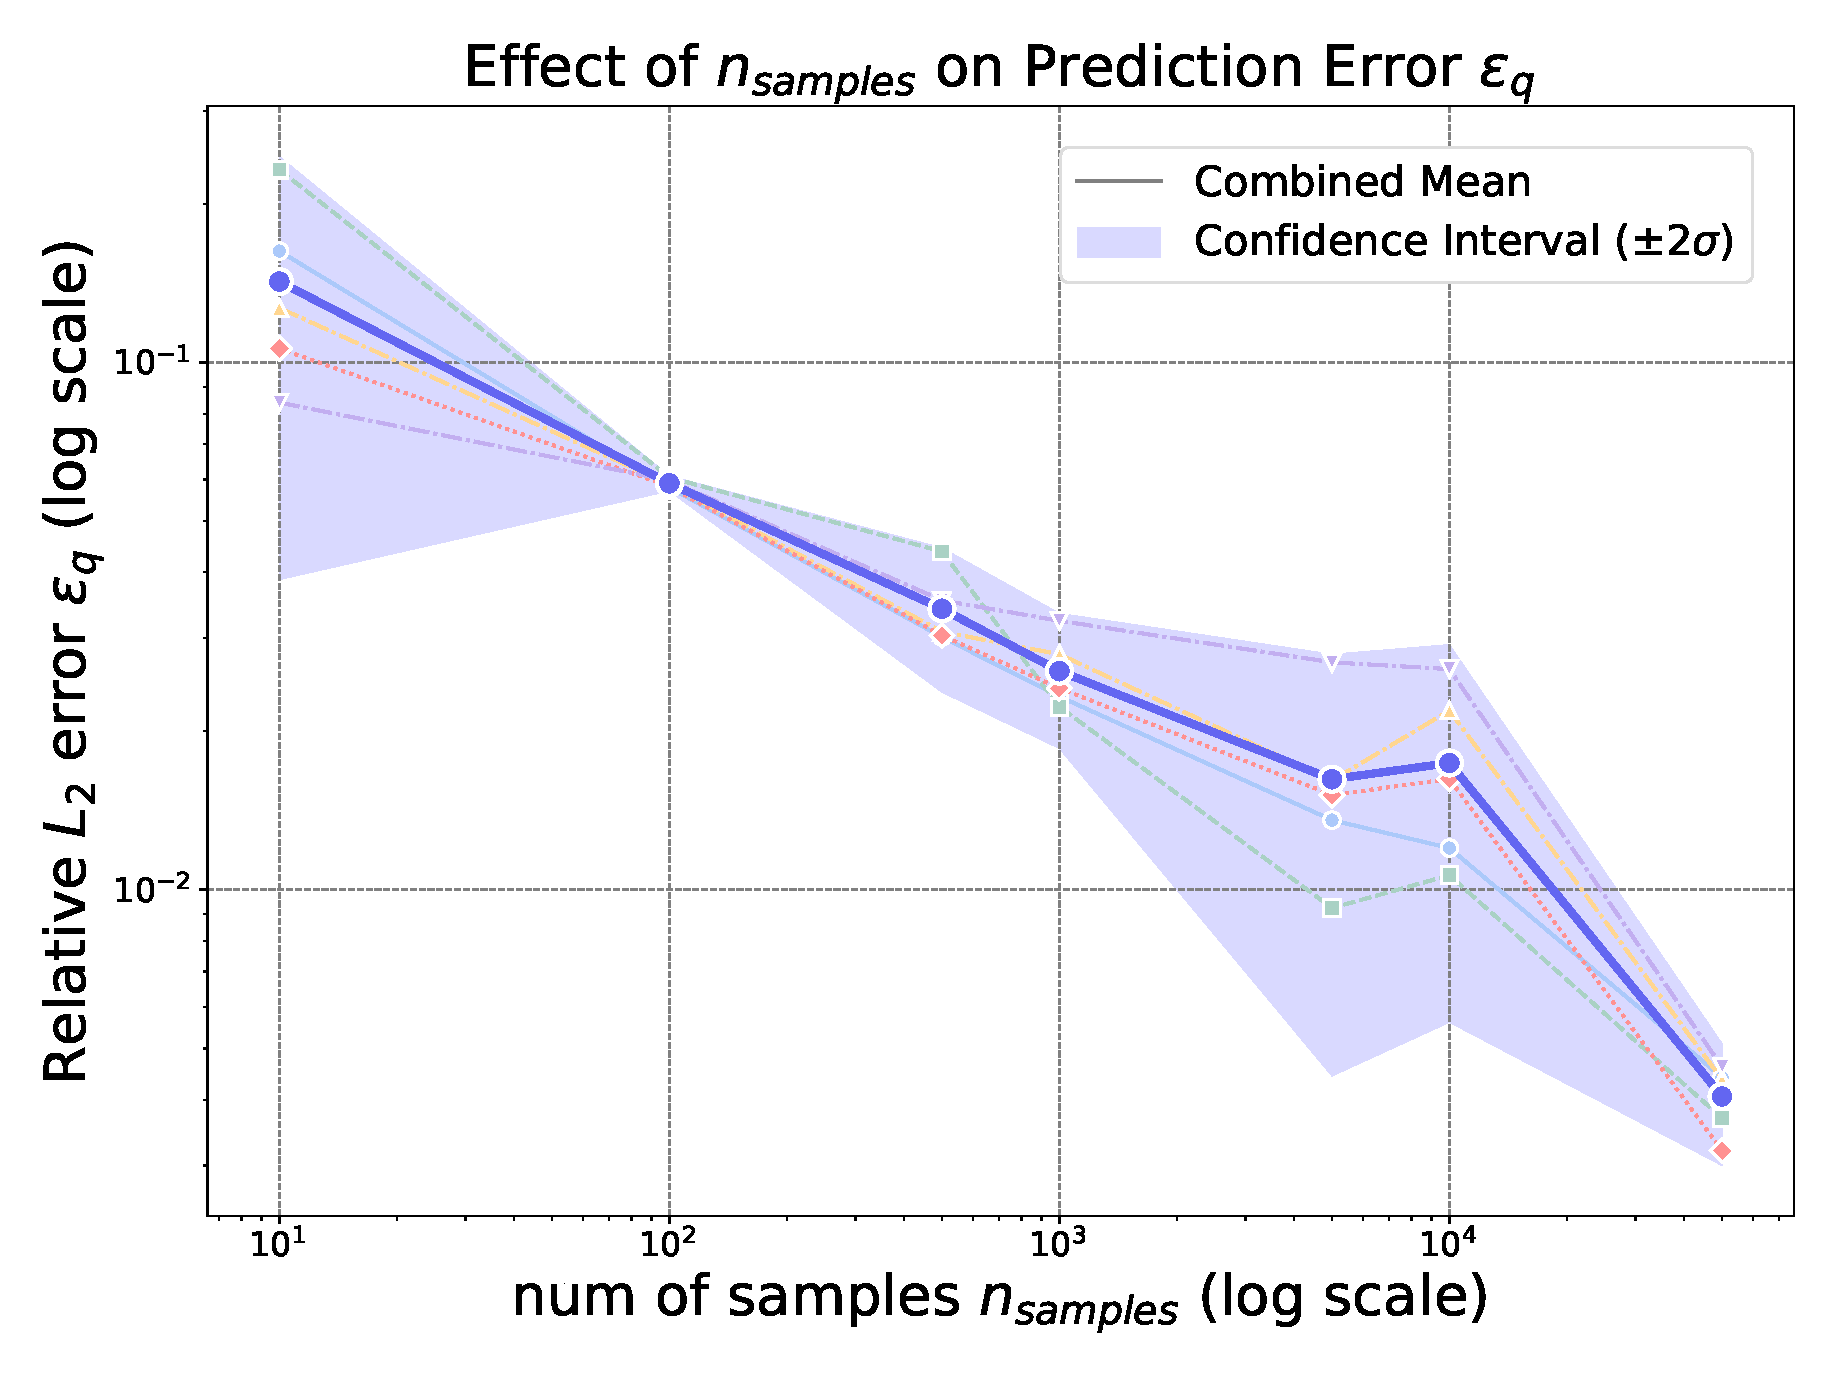
\includegraphics[width=0.48\textwidth]{figures3/ex0_nsample.eps}
%     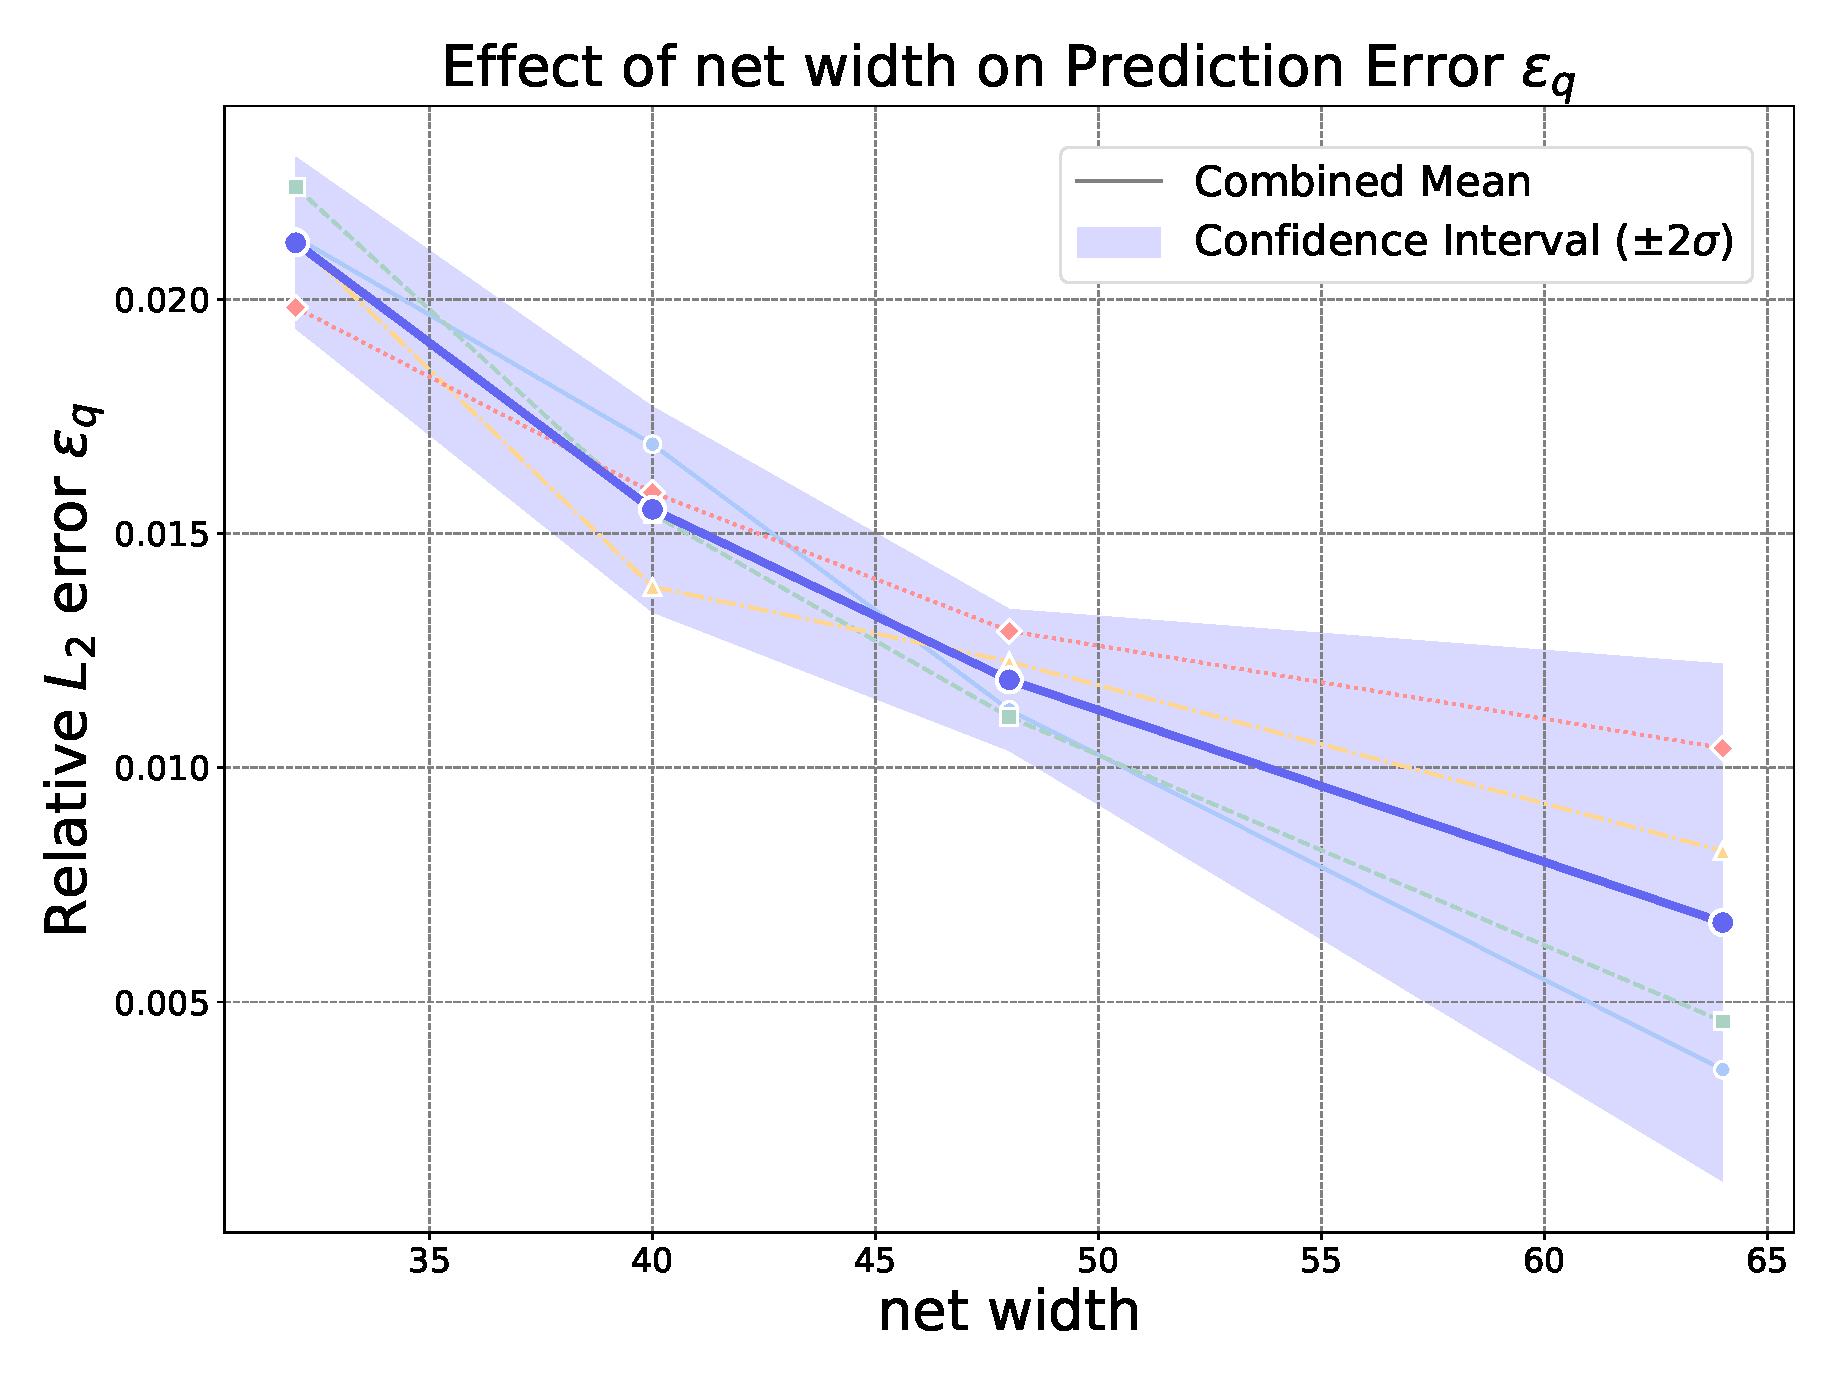
\includegraphics[width=0.48\textwidth]{figures3/ex0_width.eps}
%     \caption{样本大小和网络宽度对算法精度的影响。我们进行了多次运行，并展示了相应的置信区间。特别地，由于网络深度是固定的，非零参数的数量 $R_{\calQ}$ 与网络宽度近似成正比。}
%     \label{fig:ex0:width}
% \end{figure}

% 我们研究了神经网络复杂度和样本复杂度对模型性能的影响。根据定理 \ref{thm:ConvergenceRate} 和假设 \ref{allcondition}，要实现更低的重构误差，需要增加样本大小和网络规模。我们通过以下实验验证了这种单调关系。在图~\ref{fig:ex0:width} 左侧，我们固定网络架构并改变样本大小以考察其影响。在图~\ref{fig:ex0:width} 右侧，我们保持两层的网络深度，同时调整网络宽度，从而按比例缩放神经元总数 $R_\mathbf{\calQ}$。对每个设置都进行了多次运行，图中显示的结果表明，误差随着样本大小和参数数量的增加而减小。

% \subsubsection{二维问题}
% 接下来我们展示一个二维光滑算例，其中待反演的 $q^{\dagger}$ 和 $u^{\dagger}$ 均呈现正弦函数形式。

% \begin{example}\label{example:onemode}
% 令 $\Omega=(0,1)^{2}$ 且 $\alpha\equiv 1$。我们考虑对以下势函数的识别
% \begin{equation*}
% q^{\dagger}(x_{1},x_{2})=1+0.5\times\sin(\pi x_{1})\sin(\pi x_{2}),
% \end{equation*}
% 且精确解 $u^{\dagger}$ 为：
% \[
% u^{\dagger}(x_{1},x_{2})=1+\sin(\pi x_{1})\sin(\pi x_{2}).
% \]
% \end{example}

% 在本实验中，神经网络包含两个宽度为 64 的隐藏层。我们在内部和边界上共采样 100,000 个点，并使用学习率为 $10^{-4}$ 的 Adam 优化器训练模型 50,000 次迭代。

% 我们还使用有限元方法 (FEM) 求解了相同的问题。在 FEM 实现中，采用了一阶拉格朗日单元，并利用 L-BFGS 算法对解进行了 50 次迭代优化。为了确保比较的公平性，区域 $[0,1]^2$ 被离散化为 $320\times 320=102,400$ 个网格点，这与 Tikhonov-PINNs 中使用的总样本数（$100,000$ 个样本）相当。

% \begin{figure}[htbp]
%     \centering
%     % 第一个子图：Tikhonov-PINNs 方法（假设文件名暗示这是神经网络方法）
%     \begin{subfigure}[b]{\textwidth}
%         \centering
%         % 插入图片
%         \includegraphics[width=\textwidth]{figures3/one_peak_nn.eps}
%         % 简短的子标题
%         \caption{Tikhonov-PINNs 方法结果}
%         \label{fig:one_peak_nn}
%     \end{subfigure}
%     \hfill % 填充中间空白，让图片分别对齐左右
%     % 第二个子图：有限元方法 (FEM)
%     \begin{subfigure}[b]{\textwidth}
%         \centering
%         % 插入图片
%         \includegraphics[width=\textwidth]{figures3/one_peak_fem.eps}
%         % 简短的子标题
%         \caption{有限元方法 (FEM) 结果}
%         \label{fig:one_peak_fem}
%     \end{subfigure}
    
%     % 总标题：包含详细描述
%     \caption{两种方法重构结果的比较：(a) Tikhonov-PINNs 和 (b) 有限元方法 (FEM)。
%     左侧小图展示了例 \ref{example:onemode} 中势函数 $q^{\dagger}$（上）和解 $u^{\dagger}$（下）的真值；
%     右侧小图展示了在不同噪声水平 $\delta$ 下，使用最优正则化参数 $\lambda$ 重构的势 $\hat{q}$ 和解 $\hat{u}$。}
%     \label{fig:example:one_peak}
% \end{figure}


% 数值结果如图~\ref{fig:example:one_peak} 所示。这里，基于各种实验，$\lambda$ 被选为最优正则化参数。为了进一步阐明噪声 $\delta$ 的影响，我们在表~\ref{tab:onemode} 中提供了不同正则化参数 $\lambda$ 下相对误差的详细比较。显然，在低噪声水平下，FEM 和 Tikhonov-PINNs 方法均能有效地重构 $q$ 和 $u$。此外，随着噪声水平的增加，$q$ 的误差逐渐增大，这与我们的理论发现相符。在大多数情况下，FEM 优于 Tikhonov-PINNs 方法，当 $\lambda$ 选择得当时，产生的相对 $L^2$ 误差更低。这突显了 FEM 在处理此类光滑问题时的优越性，特别是在低维情况下。然而，正如第~\ref{sec:semi_converge} 节所讨论的，FEM 中的半收敛现象需要仔细的早停策略。此外，对于非光滑和高维问题，Tikhonov-PINNs 表现出优于标准 FEM 的性能。我们将在后续章节中对此进行讨论。

% 聚焦于 Tikhonov-PINNs 的结果，很明显，较高的噪声水平需要较大的正则化参数 $\lambda$，以在重构解中获得最佳的误差控制。噪声强度与正则化参数之间的这种单调关系与定理~\ref{thm:ConvergenceRate} 中的分析一致。

% \begin{table}[htbp]
%    \centering
%    \footnotesize
%    \caption{例 \ref{example:onemode} 中重构势 $\hat{q}$ 和解 $\hat{u}$ 的相对 $L^{2}$ 误差。}
%    \begin{tabular}{lllllll}
%    \hline
%    \multirow{2}[0]{*}{$\delta  = 1\%$} & \multicolumn{6}{c}{正则化参数 $\lambda$} \\
%    \cline{2-7}
%    & $1.0\times 10^{-5}$ & $1.0\times 10^{-6}$ & $1.0\times 10^{-7}$ & $1.0\times 10^{-8}$ & $1.0\times 10^{-9}$ & \multicolumn{1}{r}{0} \\
%    \hline
%    $\text{err}(u_{\text{pinn}})$ & $3.14\times 10^{-3}$ & $1.49\times 10^{-3}$ & $7.67\times 10^{-4}$ & $5.99\times 10^{-4}$ & $5.81\times 10^{-4}$ & $5.72\times 10^{-4}$ \\
%    $\text{err}(u_{\text{fem}})$ & $1.93\times 10^{-4}$ & $1.84\times 10^{-4}$ & $1.19\times 10^{-4}$ & $1.44\times 10^{-4}$ & $1.68\times 10^{-4}$ & $1.03\times 10^{-4}$ \\
%    $\text{err}(q_{\text{pinn}})$ & $1.46\times 10^{-1}$ & $5.39\times 10^{-2}$ & $3.39\times 10^{-2}$ & $3.27\times 10^{-2}$ & $3.27\times 10^{-2}$ & $3.27\times 10^{-2}$ \\
%    $\text{err}(q_{\text{fem}})$ & $1.44\times 10^{-2}$ & \textbf{1.23$\times $10$^{-2}$} & $6.26\times 10^{-3}$ & $1.27\times 10^{-2}$ & $1.68\times 10^{-2}$ & $1.95\times 10^{-2}$ \\
%    \hline
%    &       &       &       &       &       &  \\
%    \hline
%    \multirow{2}[0]{*}{$\delta = 10\%$} & \multicolumn{6}{c}{正则化参数 $\lambda$} \\
%    \cline{2-7}
%    & $1.0\times 10^{-5}$ & $1.0\times 10^{-6}$ & $1.0\times 10^{-7}$ & $1.0\times 10^{-8}$ & $1.0\times 10^{-9}$ & \multicolumn{1}{r}{0} \\
%    \hline
%    $\text{err}(u_{\text{pinn}})$ & $3.08\times 10^{-3}$ & $1.97\times 10^{-3}$ & $1.48\times 10^{-3}$ & $1.41\times 10^{-3}$ & $1.40\times 10^{-3}$ & $1.40\times 10^{-3}$ \\
%    $\text{err}(u_{\text{fem}})$ & $1.09\times 10^{-3}$ & $6.30\times 10^{-4}$ & $1.71\times 10^{-3}$ & $2.51\times 10^{-3}$ & $2.71\times 10^{-3}$ & $3.43\times 10^{-3}$\\
%    $\text{err}(q_{\text{pinn}})$ & $1.50\times 10^{-1}$ & $6.18\times 10^{-2}$ & $4.33\times 10^{-2}$ & $4.13\times 10^{-2}$ & $4.11\times 10^{-2}$ & $4.11\times 10^{-2}$ \\
%    $\text{err}(q_{\text{fem}})$ & \textbf{1.72$\times $10$^{-2}$} & $2.84\times 10^{-2}$ & $8.56\times 10^{-2}$ & $3.23\times 10^{-1}$ & $3.80\times 10^{-1}$ & $5.40\times 10^{-1}$\\
%    \hline
%    &       &       &       &       &       &  \\
%    \hline
%    \multirow{2}[0]{*}{$\delta = 20\%$} & \multicolumn{6}{c}{正则化参数 $\lambda$} \\
%    \cline{2-7}
%    & $1.0\times 10^{-5}$ & $1.0\times 10^{-6}$ & $1.0\times 10^{-7}$ & $1.0\times 10^{-8}$ & $1.0\times 10^{-9}$ & \multicolumn{1}{r}{0} \\
%    \hline
%    $\text{err}(u_{\text{pinn}})$ & $3.38\times 10^{-3}$ & $2.47\times 10^{-3}$ & $2.19\times 10^{-3}$ & $2.17\times 10^{-3}$ & $2.17\times 10^{-3}$ & $2.17\times 10^{-3}$ \\
%    $\text{err}(u_{\text{fem}})$ & $8.88\times 10^{-4}$ & $2.16\times 10^{-3}$ & $4.76\times 10^{-3}$ & $4.30\times 10^{-3}$ & $3.44\times 10^{-3}$ & $4.98\times 10^{-3}$ \\
%    $\text{err}(q_{\text{pinn}})$ & $1.54\times 10^{-1}$ & $7.29\times 10^{-2}$ & $6.34\times 10^{-2}$ & $6.44\times 10^{-2}$ & $6.46\times 10^{-2}$ & $6.46\times 10^{-2}$ \\
%    $\text{err}(q_{\text{fem}})$ & \textbf{1.89$\times $10$^{-2}$} & $8.56\times 10^{-2}$ & $2.64\times 10^{-1}$ & $3.85\times 10^{-1}$ & $4.35\times 10^{-1}$ & $4.98\times 10^{-1}$\\
%    \hline
%    &       &       &       &       &       &  \\
%    \hline
%    \multirow{2}[0]{*}{$\delta = 50\%$} & \multicolumn{6}{c}{正则化参数 $\lambda$} \\
%    \cline{2-7}
%    & $1.0\times 10^{-5}$ & $1.0\times 10^{-6}$ & $1.0\times 10^{-7}$ & $1.0\times 10^{-8}$ & $1.0\times 10^{-9}$ & \multicolumn{1}{r}{0} \\
%    \hline
%    $\text{err}(u_{\text{pinn}})$ & $4.14\times 10^{-3}$ & $5.22\times 10^{-3}$ & $5.20\times 10^{-3}$ & $5.22\times 10^{-3}$ & $5.22\times 10^{-3}$ & $5.22\times 10^{-3}$ \\
%    $\text{err}(u_{\text{fem}})$ & $4.90\times 10^{-3}$ & $7.22\times 10^{-3}$ & $8.26\times 10^{-3}$ & $1.01\times 10^{-2}$ & $1.40\times 10^{-2}$ & $9.21\times 10^{-3}$ \\
%    $\text{err}(q_{\text{pinn}})$ & $1.65\times 10^{-1}$ & $1.03\times 10^{-1}$ & $1.05\times 10^{-1}$ & $1.06\times 10^{-1}$ & $1.06\times 10^{-1}$ & $1.06\times 10^{-1}$ \\
%    $\text{err}(q_{\text{fem}})$ & \textbf{5.64$\times $10$^{-2}$} & $2.32\times 10^{-1}$ & $5.85\times 10^{-1}$ & $0.85\times 10^{-1}$ & $1.10$ & $0.81\times 10^{-1}$\\
%    \hline
%    \end{tabular}
%    \label{tab:onemode}%
% \end{table}%

% \subsection{非光滑势问题}
% 为了进一步探索我们算法的局限性并评估神经网络对非光滑势的逼近能力，我们将我们的方法应用于几个非光滑算例，在这些算例中，诸如标准有限元方法 (FEM) 等传统方法的效果可能较差。参数设置保持与算例~\ref{example:onemode} 中相同。此外，我们将 Tikhonov-PINNs 方法的性能与经典有限元方法进行了比较。本节的 FEM 设置与算例 5.2 中的设置相同。

% \subsubsection{连续问题}
% 接下来，我们考虑如下定义的非光滑势函数的识别问题。

% \begin{example}\label{example:nonsmooth}
% % Table generated by Excel2LaTeX from sheet '5'
% 令 $\Omega=(0,1)^{2}$ 且 $\alpha\equiv 1$。定义精确势函数 $q^{\dagger}$ 为：
% \begin{align*}
% \zeta(x_{1},x_{2})&=\exp\{-25\times(x_{1}-0.6)^{2}-25\times(x_{2}-0.4)^{2}\}, \\
% q^{\dagger}(x_{1},x_{2})&=0.75+\min\{0.75,\max\{0.25,2\zeta(x_{1},x_{2})\}\},
% \end{align*}
% 精确解 $u^{\dagger}$ 为 $u^{\dagger}(x_{1},x_{2})=1+\sin(\pi x_{1})\sin(\pi x_{2})$。
% \end{example}
% 表 \ref{tab:nonsmooth} 展示了在不同 $\lambda$ 和 $\delta$ 下 $u$ 和 $q$ 的相对误差，并用粗体高亮了每种噪声水平下的最佳结果。正如我们所见，Tikhonov-PINNs 在所有配置下始终实现了约为 $\calO(10^{-2})$ 的 $q$ 相对误差，比有限元方法高出一个数量级。


% \begin{table}[htbp]
%    \centering
%    \footnotesize
%    \caption{Example \ref{example:nonsmooth} 中恢复的势 $\hat{q}$ 和解 $\hat{u}$ 的相对 $L^{2}$ 误差。}
%    \begin{tabular}{lllllll}
%    \hline
%    \multirow{2}[0]{*}{$\delta  = 1\%$} & \multicolumn{6}{c}{正则化参数 $\lambda$} \\
%    \cline{2-7}
%    & $1.0\times 10^{-5}$ & $1.0\times 10^{-6}$ & $1.0\times 10^{-7}$ & $1.0\times 10^{-8}$ & $1.0\times 10^{-9}$ & \multicolumn{1}{r}{0} \\
%    \hline
%    $\text{err}(u_{\text{pinn}})$ & $3.14\times 10^{-3}$ & $2.01\times 10^{-3}$ & $6.03\times 10^{-4}$ & $5.71\times 10^{-4}$ & $4.94\times 10^{-4}$ & $4.03\times 10^{-4}$ \\
%    $\text{err}(u_{\text{fem}})$& $2.60\times 10^{-3}$& $1.14\times 10^{-3}$& $7.09\times 10^{-4}$& $6.96\times 10^{-4}$ & $5.33\times 10^{-4}$ &$6.41\times 10^{-4}$\\
%    $\text{err}(q_{\text{pinn}})$ & $1.46\times 10^{-1}$& $9.63\times 10^{-2}$ & $1.82\times 10^{-2}$ & $1.60\times 10^{-2}$ & \textbf{1.57$\times$ 10$^{-2}$} & \textbf{1.57$\times$ 10$^{-2}$}   \\
%    $\text{err}(q_{\text{fem}})$& $1.28\times 10^{-1}$& $8.77\times 10^{-2}$& $7.39\times 10^{-2}$& $7.36\times 10^{-2}$ & $6.43\times 10^{-2}$ &$6.97\times 10^{-2}$\\
%    \hline
%    &       &       &       &       &       &  \\
%    \hline
%    \multirow{2}[0]{*}{$\delta = 10\%$} & \multicolumn{6}{c}{正则化参数 $\lambda$} \\
%    \cline{2-7}
%    & $1.0\times 10^{-5}$ & $1.0\times 10^{-6}$ & $1.0\times 10^{-7}$ & $1.0\times 10^{-8}$ & $1.0\times 10^{-9}$ & \multicolumn{1}{r}{0} \\
%    \hline
%    $\text{err}(u_{\text{pinn}})$ & $3.08\times 10^{-3}$ & $2.22\times 10^{-3}$ & $1.36\times 10^{-3}$ & $1.30\times 10^{-3}$ & $1.30\times 10^{-3}$ & $1.30\times 10^{-3}$ \\
%    $\text{err}(u_{\text{fem}})$& $2.82\times 10^{-3}$& $1.30\times 10^{-3}$& $1.44\times 10^{-3}$& $1.18\times 10^{-3}$ & $1.30\times 10^{-3}$&$2.36\times 10^{-3}$\\
%    $\text{err}(q_{\text{pinn}})$ & $1.50\times 10^{-1}$ & $1.03\times 10^{-1}$ & $1.78\times 10^{-2}$ & $1.60\times 10^{-2}$ & $1.71\times 10^{-2}$ & \textbf{1.58$\times$ 10$^{-2}$ }\\
%    $\text{err}(q_{\text{fem}})$& $1.29\times 10^{-1}$& $8.77\times 10^{-2}$& $7.95\times 10^{-2}$& $9.02\times 10^{-2}$ & $1.16\times 10^{-1}$&$1.90\times 10^{-1}$\\
%    \hline
%    &       &       &       &       &       &  \\
%    \hline
%    \multirow{2}[0]{*}{$\delta = 20\%$} & \multicolumn{6}{c}{正则化参数 $\lambda$} \\
%    \cline{2-7}
%    & $1.0\times 10^{-5}$ & $1.0\times 10^{-6}$ & $1.0\times 10^{-7}$ & $1.0\times 10^{-8}$ & $1.0\times 10^{-9}$ & \multicolumn{1}{r}{0} \\
%    \hline
%    $\text{err}(u_{\text{pinn}})$ & $3.38\times 10^{-3}$ & $2.30\times 10^{-3}$ & $1.44\times 10^{-3}$ & $1.35\times 10^{-3}$ & $1.36\times 10^{-3}$ & $1.36\times 10^{-3}$ \\
%    $\text{err}(u_{\text{fem}})$& $2.67\times 10^{-3}$& $2.17\times 10^{-3}$& $4.23\times 10^{-3}$&$ 3.75\times 10^{-3}$ & $2.50\times 10^{-3}$&$4.15\times 10^{-3}$\\
%    $\text{err}(q_{\text{pinn}})$ & $1.54\times 10^{-1}$ & $9.09\times 10^{-2}$ & $1.71\times 10^{-2}$ & $1.60\times 10^{-2}$ & \textbf{1.59$\times$ 10$^{-2}$} & \textbf{1.59$\times$ 10$^{-2}$} \\
%    $\text{err}(q_{\text{fem}})$& $1.27\times 10^{-1}$& $9.77\times 10^{-2}$& $2.21\times 10^{-1}$& $2.13\times 10^{-1}$ & $1.51\times 10^{-1}$&$3.79\times 10^{-1}$\\
%    \hline
%    &       &       &       &       &       &  \\
%    \hline
%    \multirow{2}[0]{*}{$\delta = 50\%$} & \multicolumn{6}{c}{正则化参数 $\lambda$} \\
%    \cline{2-7}
%    & $1.0\times 10^{-5}$ & $1.0\times 10^{-6}$ & $1.0\times 10^{-7}$ & $1.0\times 10^{-8}$ & $1.0\times 10^{-9}$ & \multicolumn{1}{r}{0} \\
%    \hline
%    $\text{err}(u_{\text{pinn}})$ & $4.14\times 10^{-3}$ & $4.43\times 10^{-3}$ & $4.07\times 10^{-3}$ & $3.43\times 10^{-3}$ & $4.01\times 10^{-3}$ & $4.04\times 10^{-3}$ \\
%    $\text{err}(u_{\text{fem}})$& $4.41\times 10^{-3}$& $7.14\times 10^{-3}$& $7.90\times 10^{-3}$& $7.64\times 10^{-3}$& $1.26\times 10^{-2}$&$8.40\times 10^{-3}$\\
%    $\text{err}(q_{\text{pinn}})$ & $1.65\times 10^{-1}$ & $1.22\times 10^{-1}$ & $6.30\times 10^{-2}$ & \textbf{3.16}$\times$ \textbf{10}$^{-2}$ & $4.99\times 10^{-2}$ & $5.14\times 10^{-1}$ \\
%    $\text{err}(q_{\text{fem}})$& $1.45\times 10^{-1}$& $2.14\times 10^{-1}$& $4.64\times 10^{-1}$& $4.09\times 10^{-1}$& $9.07\times 10^{-1}$&$5.90\times 10^{-1}$\\
%    \hline
%    \end{tabular}%
%    \label{tab:nonsmooth}%
% \end{table}%

% \begin{figure}[htbp]
% \centering
% \setlength{\abovecaptionskip}{10pt}
% 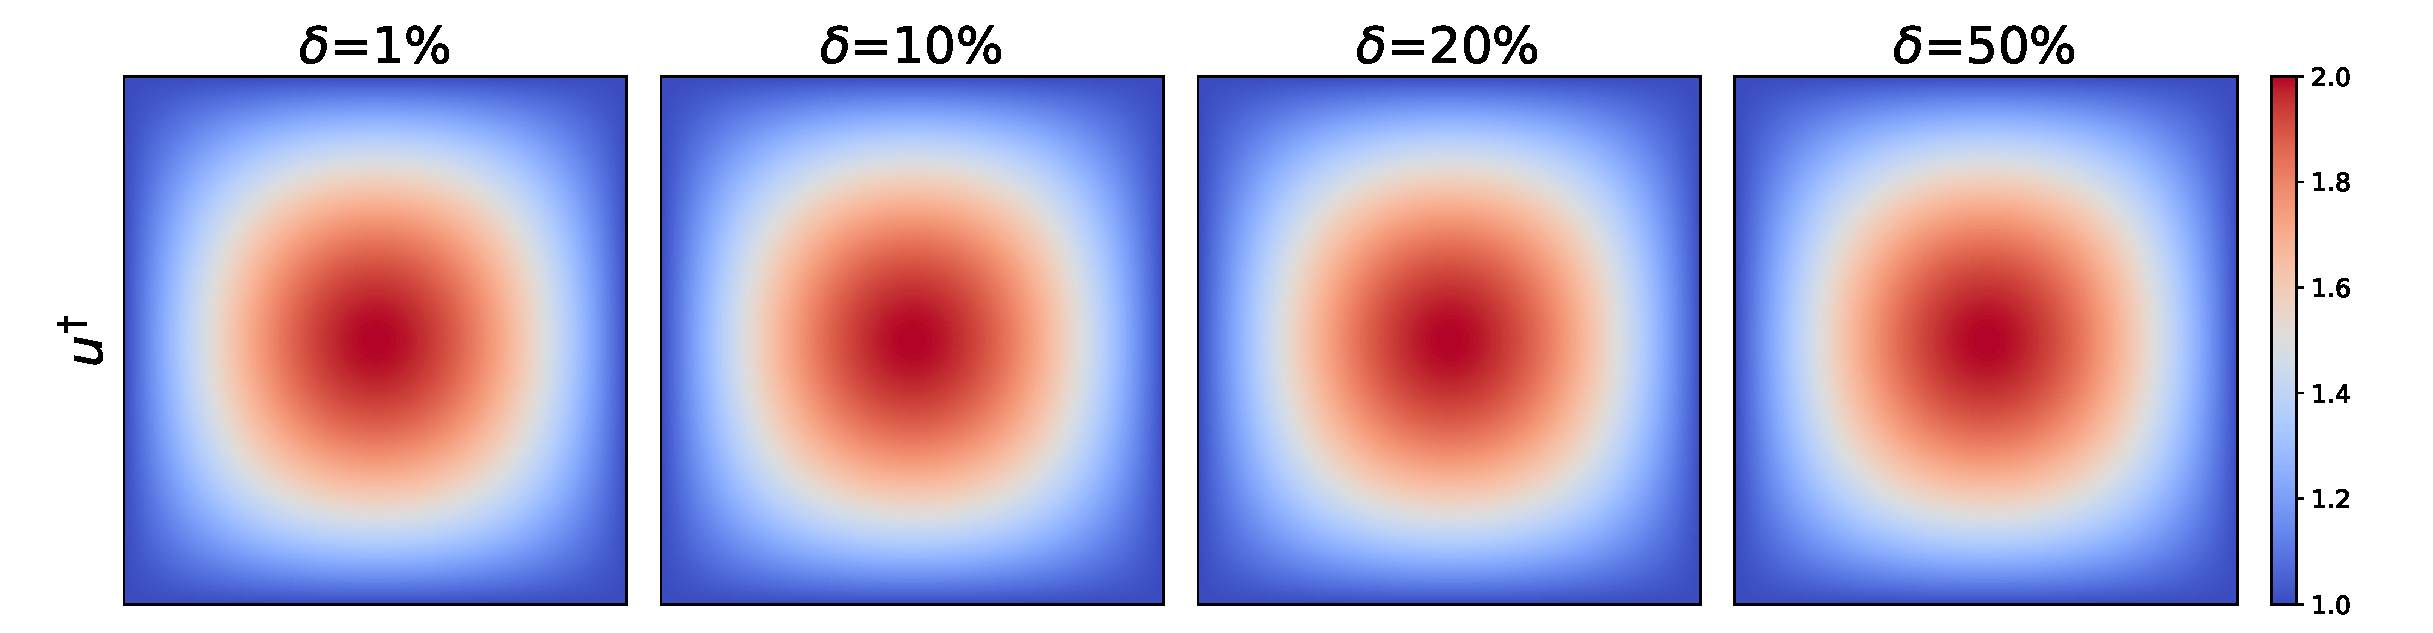
\includegraphics[width=\textwidth]{figures3/non_smooth_udag.eps}\par
% 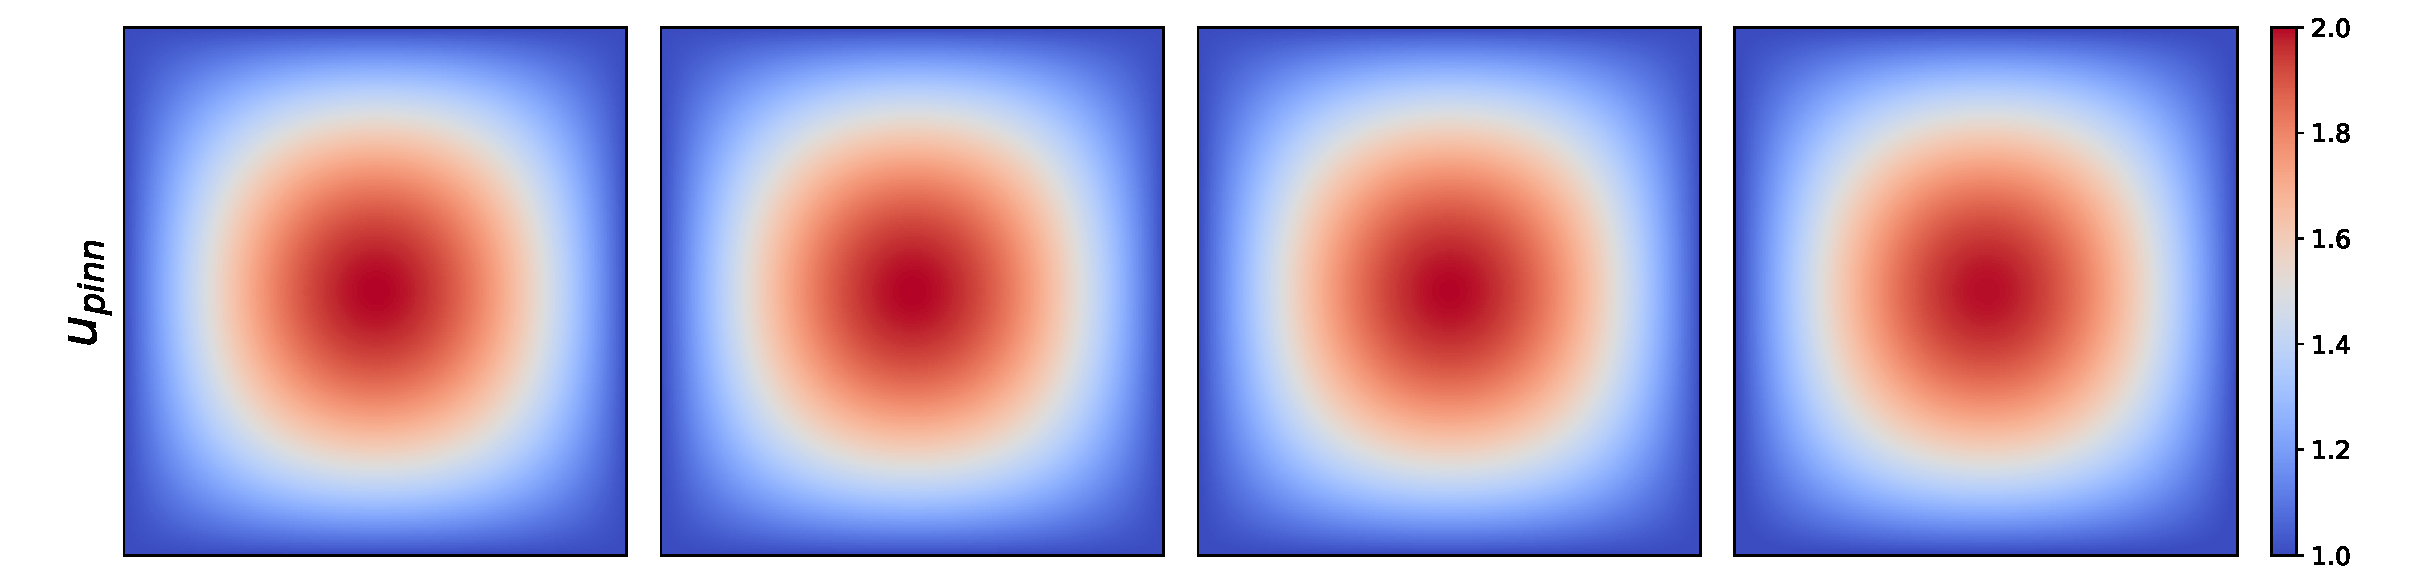
\includegraphics[width=\textwidth]{figures3/non_smooth_unn.eps}\par
% 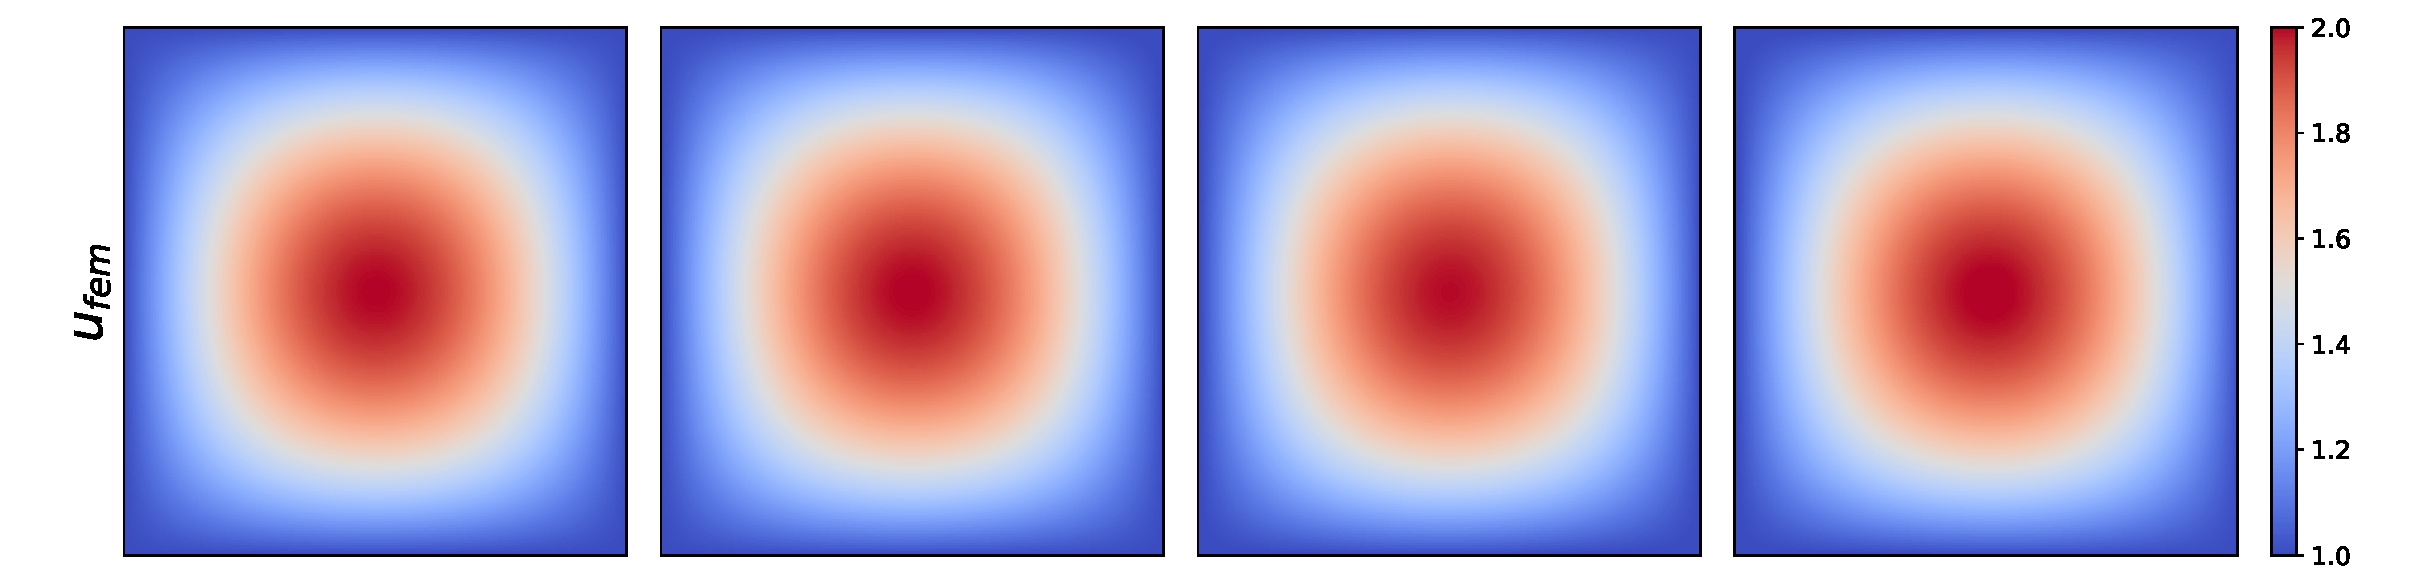
\includegraphics[width=\textwidth]{figures3/non_smooth_ufem.eps}\par
% 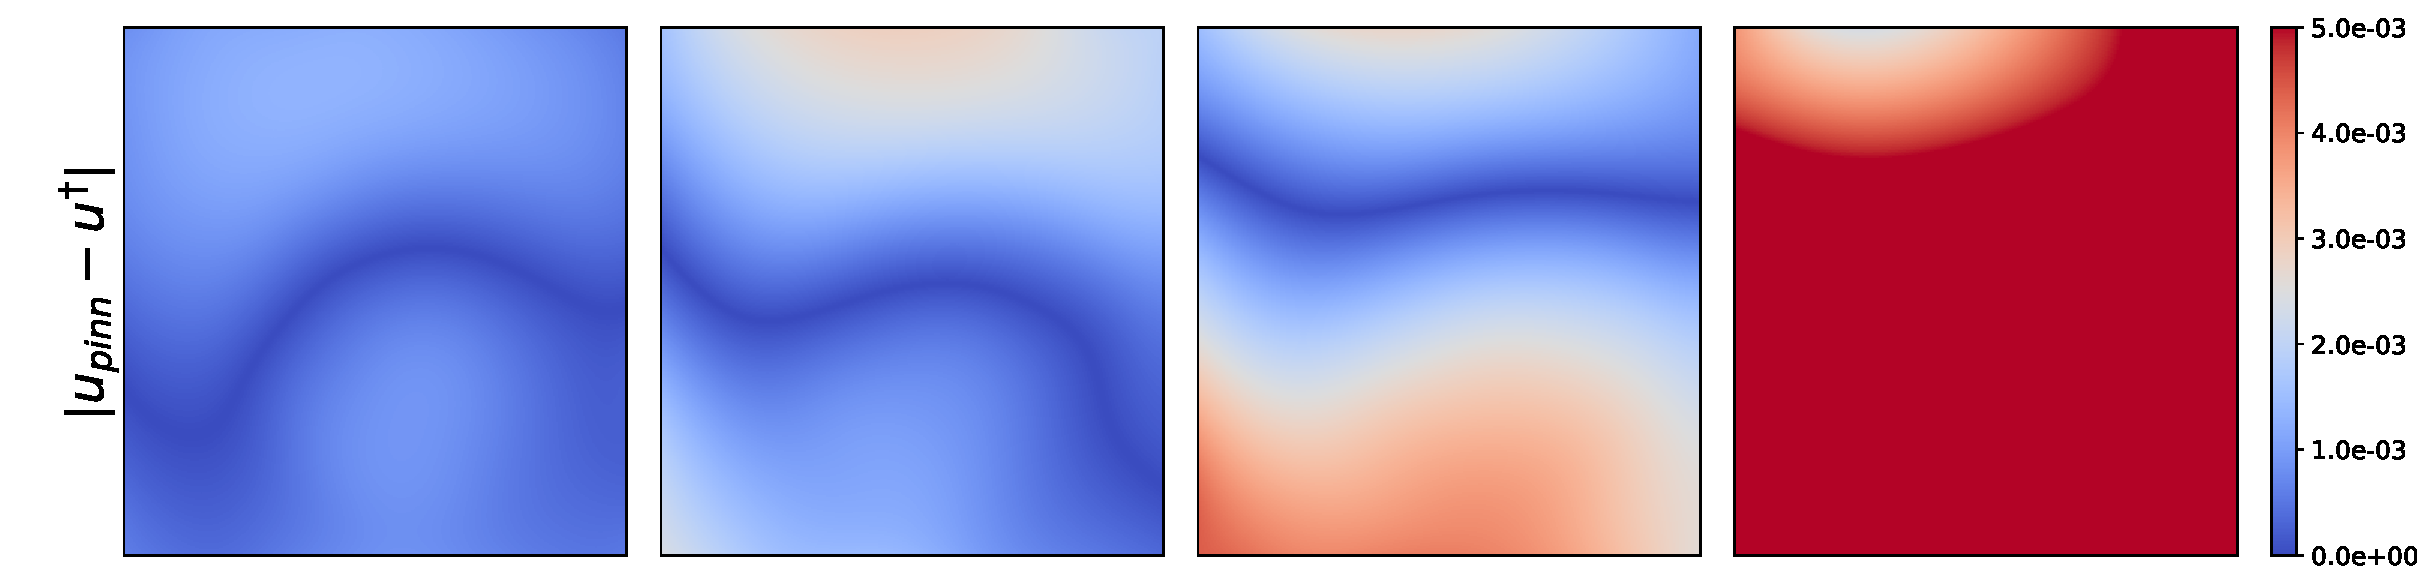
\includegraphics[width=\textwidth]{figures3/non_smooth_unn_err.eps}\par
% 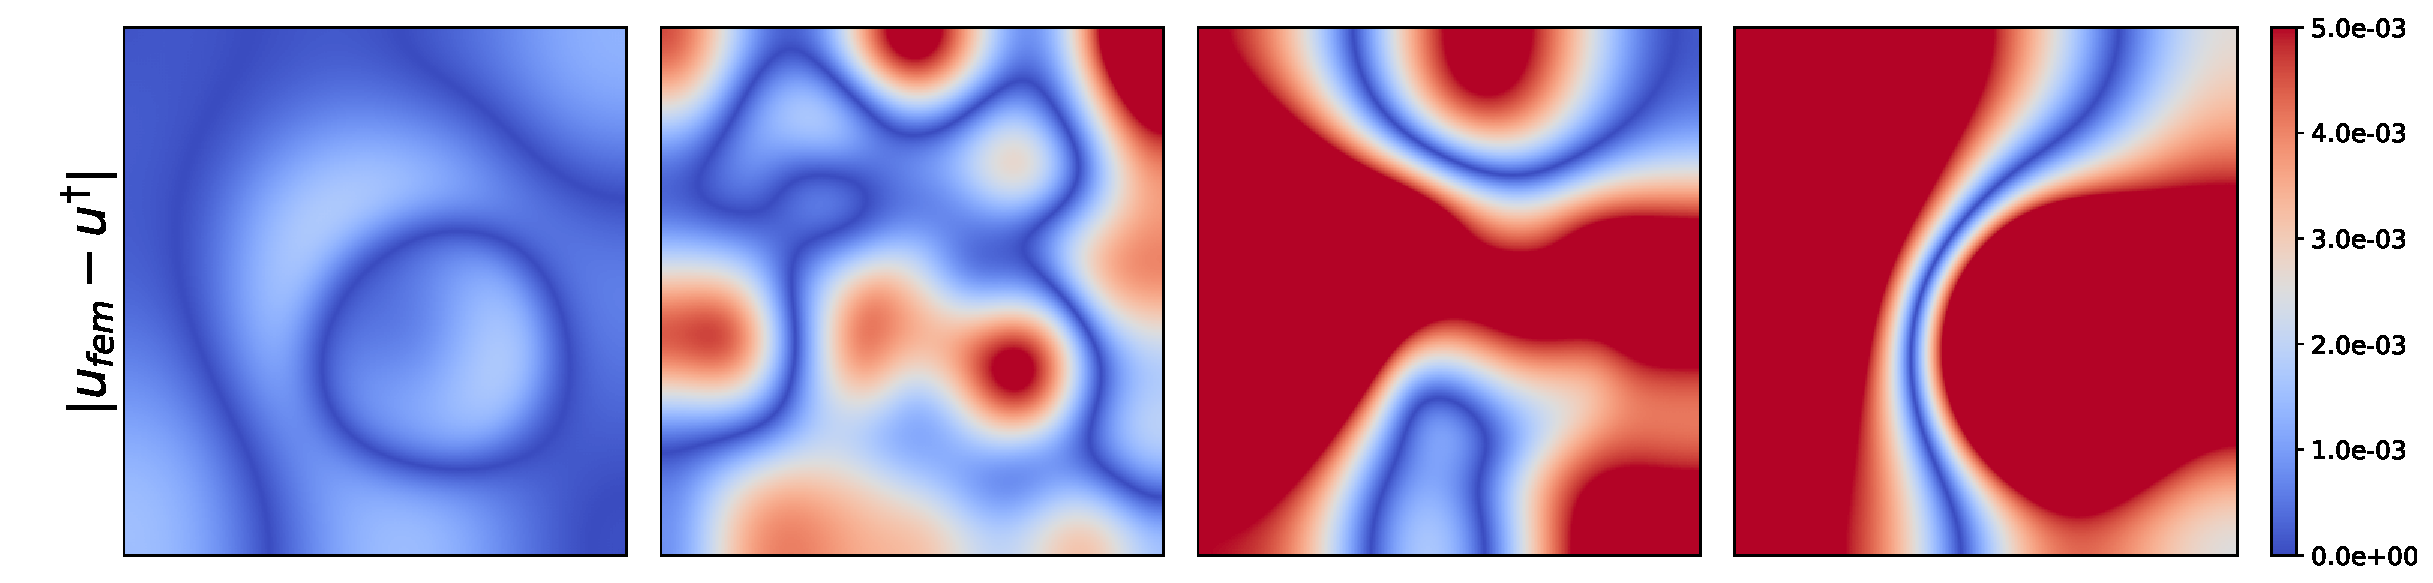
\includegraphics[width=\textwidth]{figures3/non_smooth_ufem_err.eps}
% \caption{从上到下依次为：Example \ref{example:nonsmooth} 中的真实势函数 $u^{\dagger}$，由 Tikhonov-PINNs 恢复的势函数 $u_{\text{pinn}}$，逐点绝对误差 $|u^{\dagger}-u_{\text{pinn}}|$，由 FEM 恢复的势函数 $u_{\text{fem}}$，逐点绝对误差 $|u^{\dagger}-u_{\text{fem}}|$。我们绘制了不同噪声水平下的结果。}
% \label{fig:example:nonsmooth:u}
% \end{figure}

% \begin{figure}[htbp]
% \centering
% \setlength{\abovecaptionskip}{10pt}
% 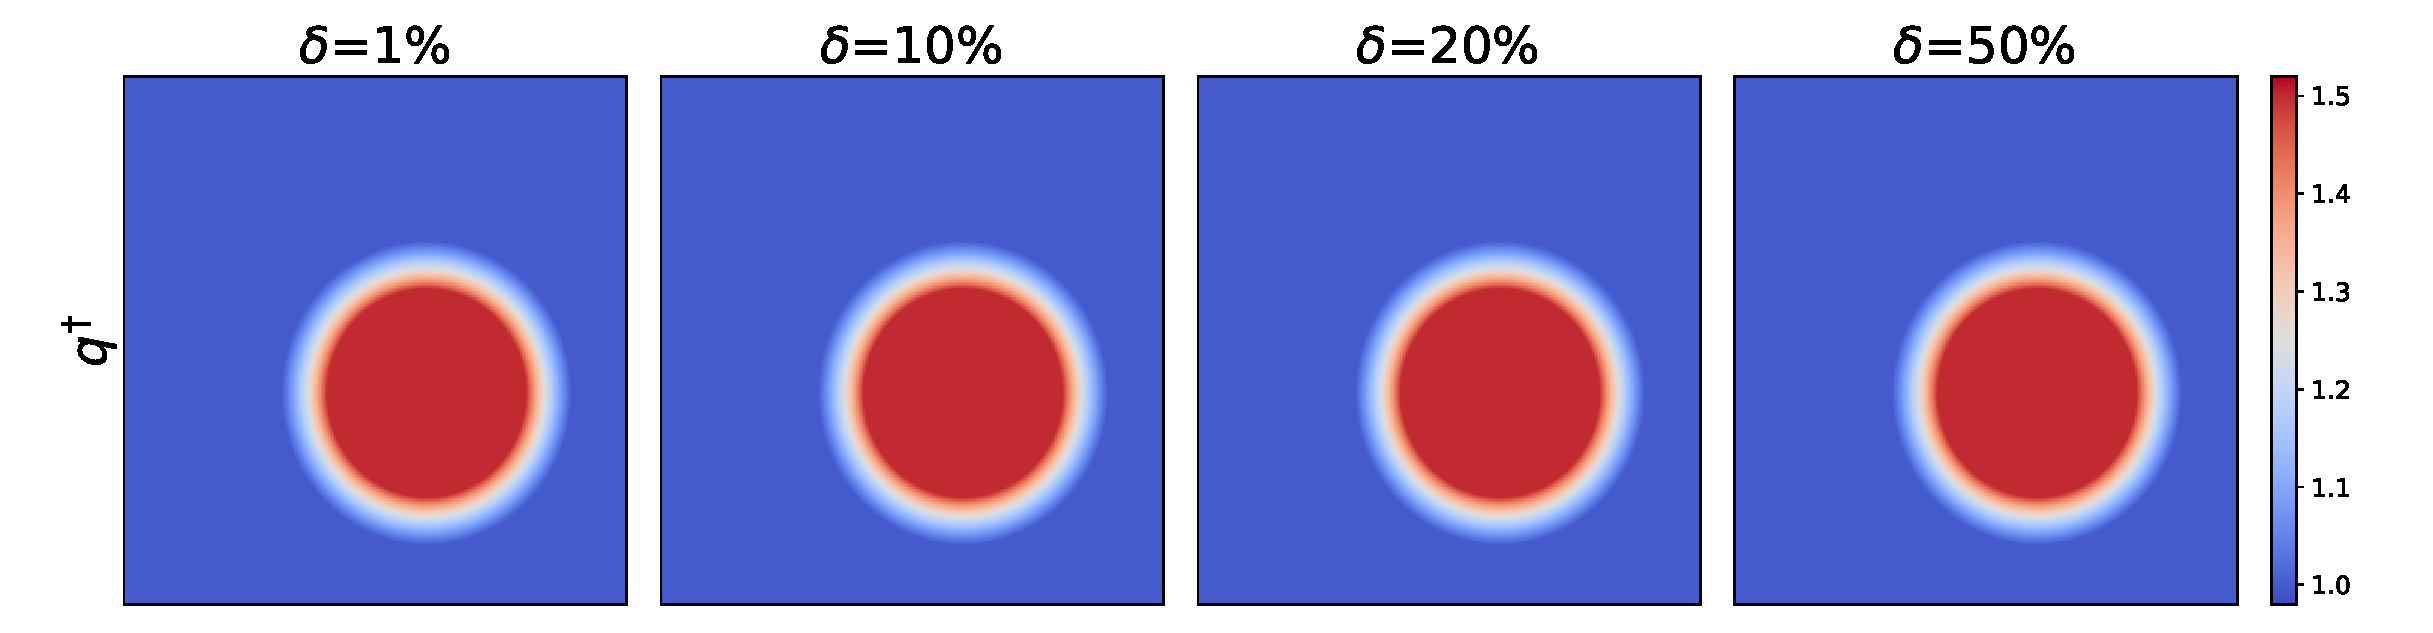
\includegraphics[width=\textwidth]{figures3/non_smooth_qdag.eps}\par
% 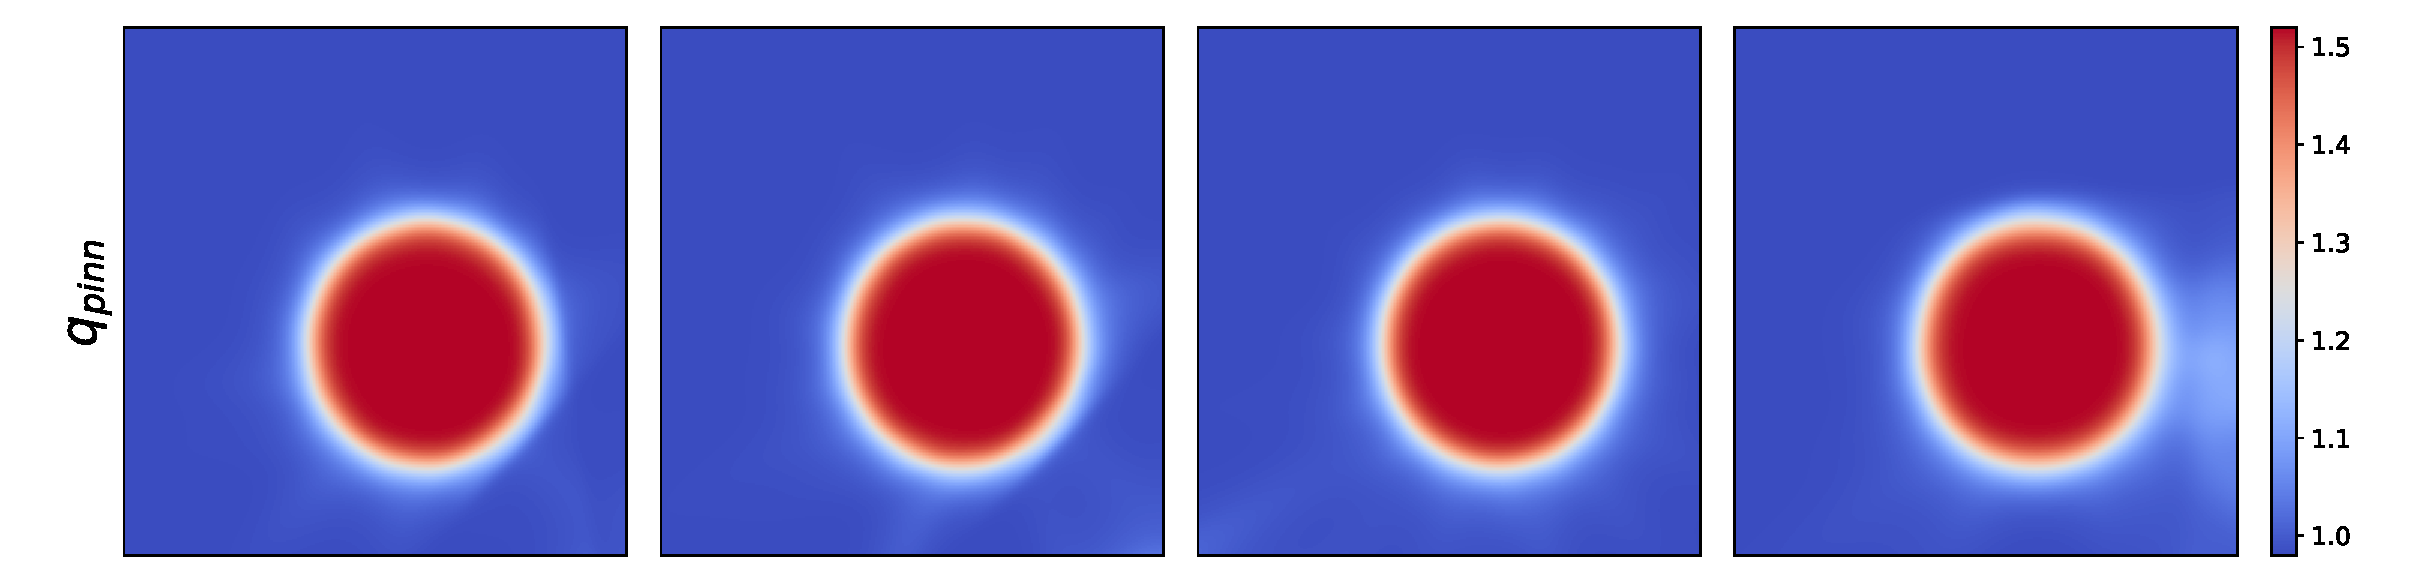
\includegraphics[width=\textwidth]{figures3/non_smooth_qnn.eps}\par
% 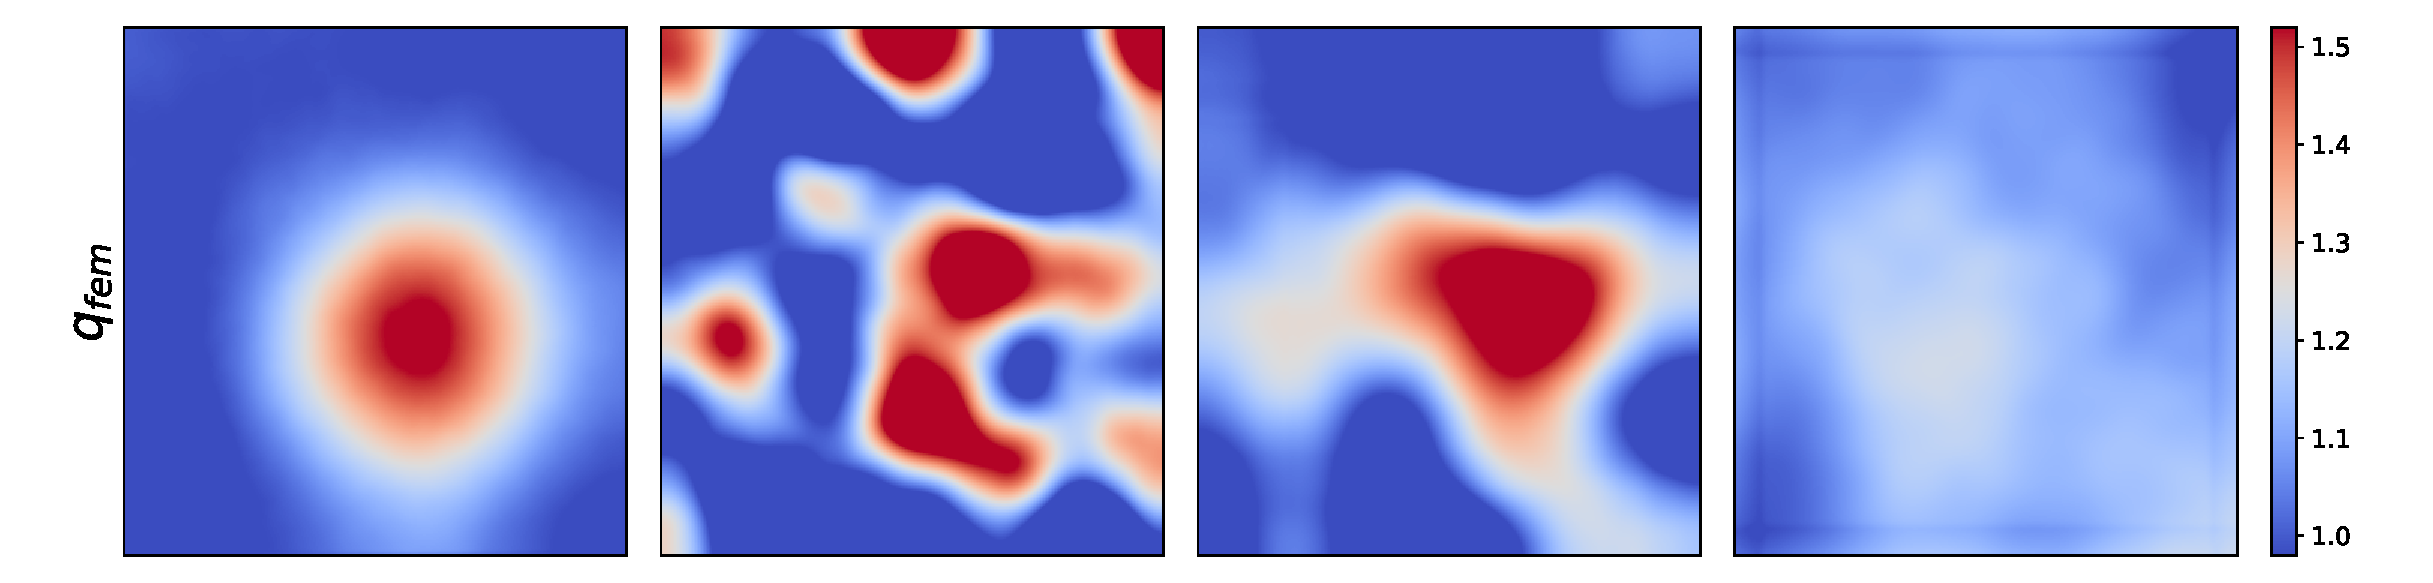
\includegraphics[width=\textwidth]{figures3/non_smooth_q_fem.eps}\par
% 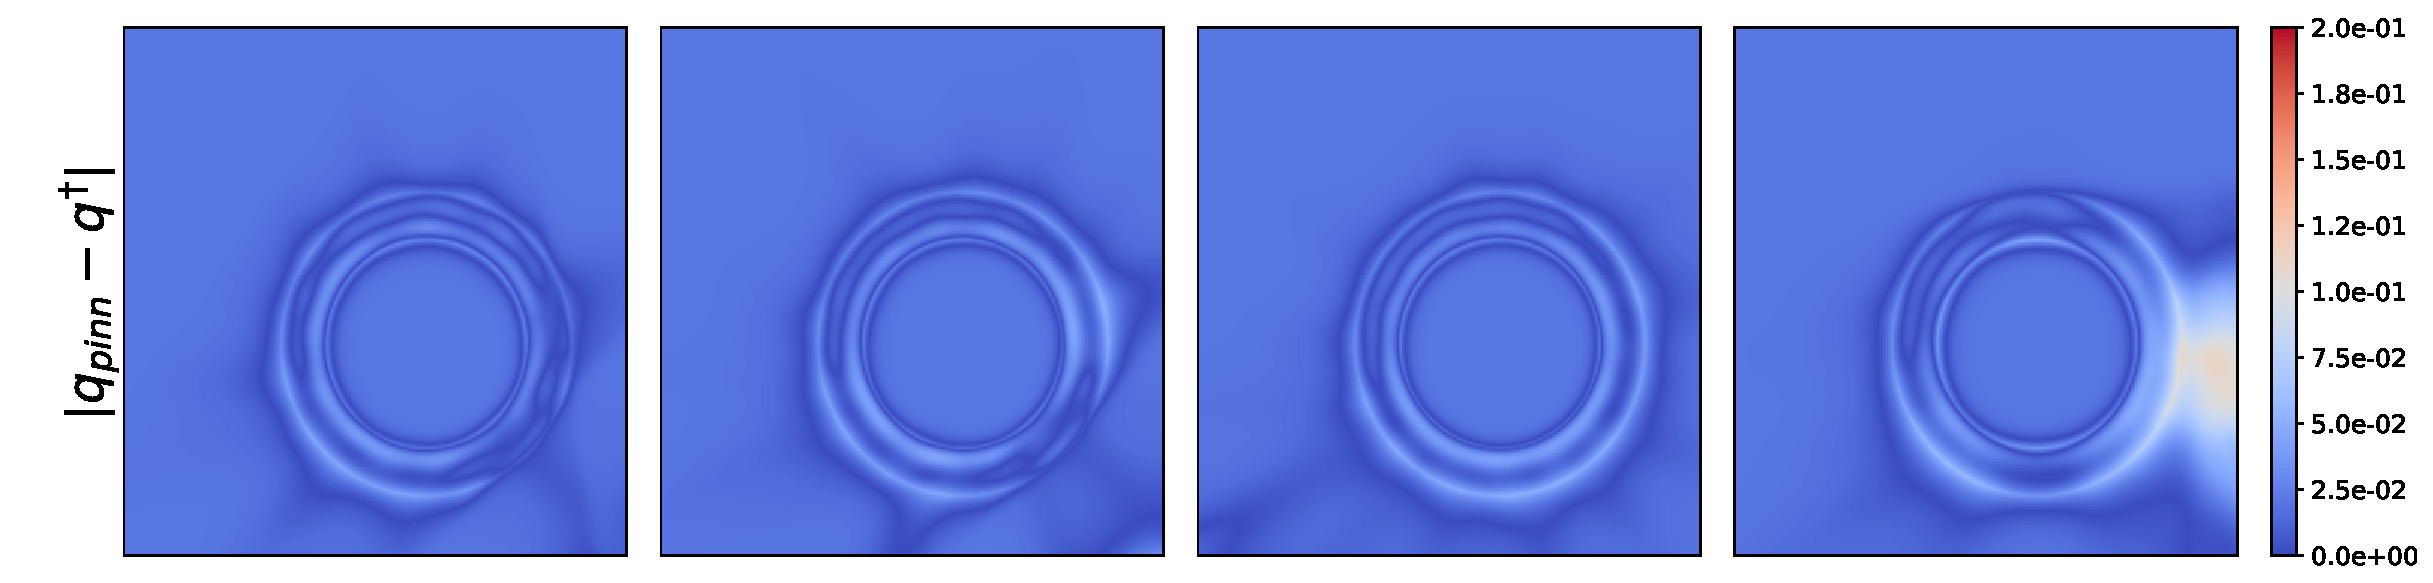
\includegraphics[width=\textwidth]{figures3/non_smooth_qnn_err.eps}\par
% 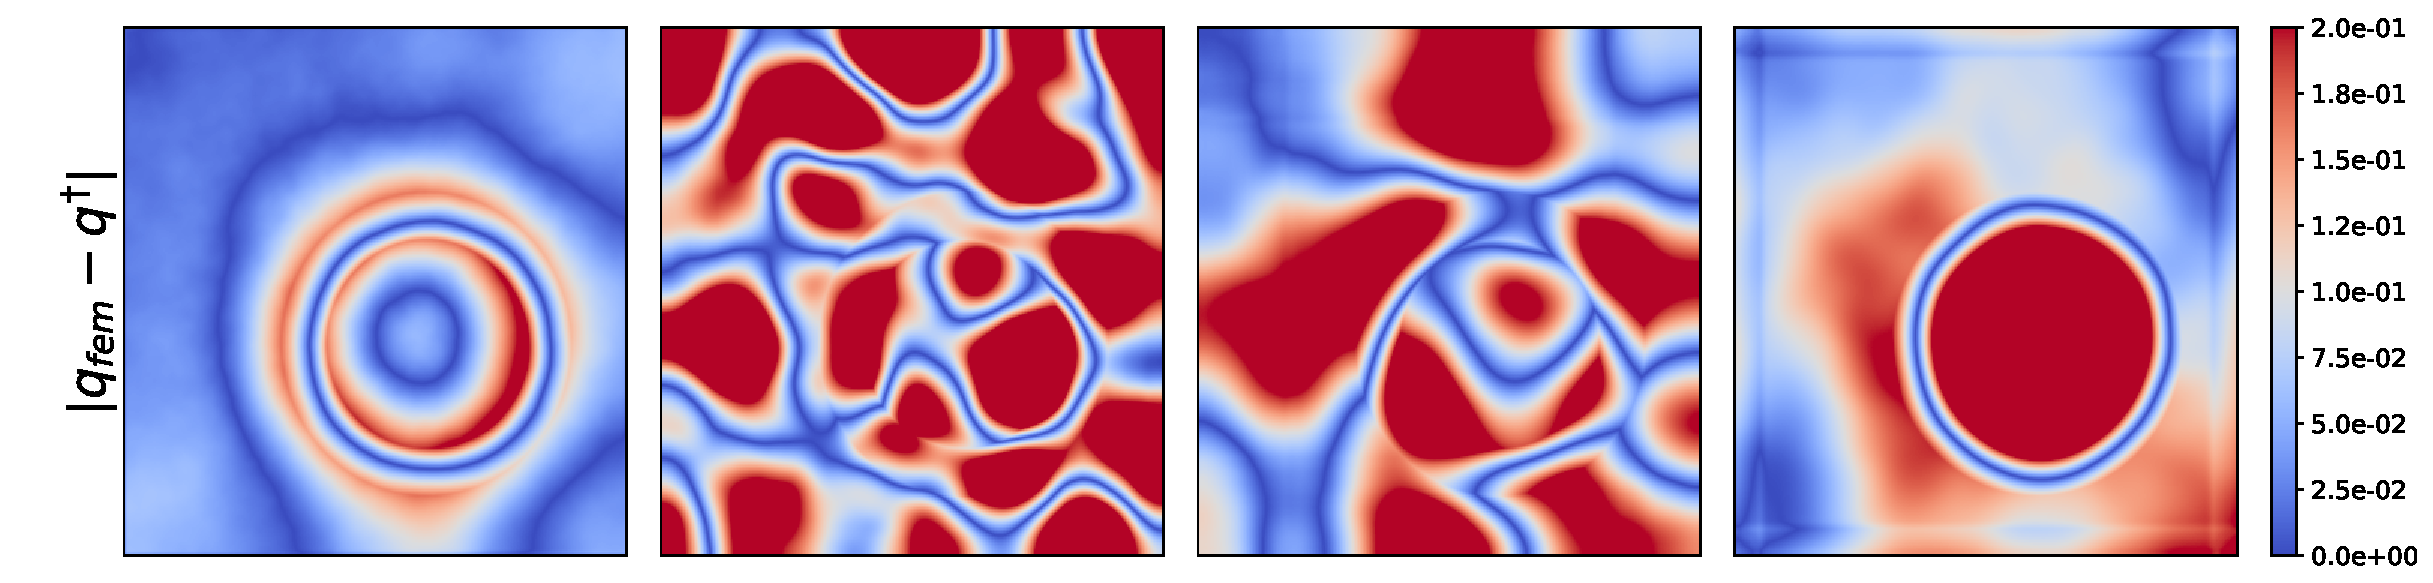
\includegraphics[width=\textwidth]{figures3/non_smooth_qfem_err.eps}
% \caption{从上到下依次为：Example \ref{example:nonsmooth} 中的真实势函数 $q^{\dagger}$，由 Tikhonov-PINNs 恢复的势函数 $q_{\text{pinn}}$，逐点绝对误差 $|q^{\dagger}-q_{\text{pinn}}|$，由 FEM 恢复的势函数 $q_{\text{fem}}$，逐点绝对误差 $|q^{\dagger}-q_{\text{fem}}|$。我们绘制了不同噪声水平下的结果。}
% \label{fig:example:nonsmooth}
% \end{figure}

% 在本例中，势函数 $q^{\dagger}$ 呈现出一种平台结构：它在红圈内部和蓝圈外部均保持常数。如图 \ref{fig:example:nonsmooth:u} 和图 \ref{fig:example:nonsmooth} 所示，重构 $u$ 相对简单，Tikhonov-PINNs 和基于有限元的方法均表现良好。然而，在重构 $q$ 时，Tikhonov-PINNs 成功捕捉到了常数值区域，而有限元方法未能精确识别 $q$ 中的界面，导致误差显著偏高。即使在高噪声水平下（例如 $\delta = 50\%$），我们的方法仍能恢复势函数的整体结构，而有限元方法几乎产生不了任何有意义的信息。

% \subsubsection{不连续问题}

% 作为第三个例子，我们将求解一个不连续势函数的反问题。
% \begin{example}\label{example:discontinuous}
% 令 $\Omega=(0,1)^{2}$ 且 $\alpha\equiv 1$。定义精确势函数 $q^{\dagger}$ 为：
% \begin{align*}
% \zeta(x_{1},x_{2})&=\exp\{-9\times(x_{1}-0.5)^{2}-9\times(x_{2}-0.5)^{2}\}, \\
% q^{\dagger}(x_{1},x_{2})&=1.0+0.5\times\zeta(x_{1},x_{2})\chi_{\{x_{1}\geq x_{2}\}},
% \end{align*}
% 精确解 $u^{\dagger}$ 为：$u^{\dagger}(x_{1},x_{2})=1+\sin(\pi x_{1})\sin(\pi x_{2})$。
% \end{example}

% \begin{table}[hbtp]
% \centering
% \footnotesize
% \caption{例 \ref{example:discontinuous} 中恢复的势函数 $\hat{q}$ 和解 $\hat{u}$ 的相对 $L^{2}$ 误差。}
% \begin{tabular}{lrrrrrr}
% \hline
% \multirow{2}[0]{*}{$\delta $ = 1\%} & \multicolumn{6}{c}{正则化参数 $\lambda$} \\
% \cline{2-7}
% & \multicolumn{1}{l}
% {$1.0\times 10^{-5}$} & 
% \multicolumn{1}{l}{$1.0\times 10^{-6}$} &
% \multicolumn{1}{l}{$1.0\times 10^{-7}$} &
% \multicolumn{1}{l}{$1.0\times 10^{-8}$} & 
%    \multicolumn{1}{l}{$1.0\times 10^{-9}$} & {0} \\
%    \hline
% $\text{err}(u_{\text{pinn}})$ & $2.05\times 10^{-3}$ & $1.54\times 10^{-3}$ & $1.07\times 10^{-3}$ & $9.83\times 10^{-4}$ & $7.55\times 10^{-4}$ & $6.42\times 10^{-4}$ \\
% $\text{err}(u_{\text{fem}})$&$1.46\times 10^{-3}$ & $7.05\times 10^{-4}$ & $4.80\times 10^{-4}$ & $2.66\times 10^{-4}$ & $2.50\times 10^{-4}$ & $2.38\times 10^{-4}$\\
% $\text{err}(q_{\text{pinn}})$ & $9.82\times 10^{-2}$ & $8.50\times 10^{-2}$ & $6.76\times 10^{-2}$ & $5.23\times 10^{-2}$ & $3.49\times 10^{-2}$ & \textbf{2.79$\times$ 10$^{-2}$} \\
% $\text{err}(q_{\text{fem}})$&$8.42\times 10^{-2}$ & $6.36\times 10^{-2}$ & $5.62\times 10^{-2}$ & $4.84\times 10^{-2}$ & $4.53\times 10^{-2}$ & $4.55\times 10^{-2}$\\
% \hline
% &       &       &       &       &       &  \\
% \hline
% \multirow{2}[0]{*}{$\delta$ = 10\%} & \multicolumn{6}{c}{正则化参数 $\lambda$} \\
% \cline{2-7}
% & $1.0\times 10^{-5}$ & $1.0\times 10^{-6}$ & $1.0\times 10^{-7}$ & $1.0\times 10^{-8}$ & $1.0\times 10^{-9}$ & \multicolumn{1}{r}{0} \\
% \hline
% $\text{err}(u_{\text{pinn}})$ & $1.96\times 10^{-3}$ & $1.74\times 10^{-3}$ & $1.38\times 10^{-3}$ & $1.12\times 10^{-3}$ & $1.49\times 10^{-3}$ & $1.48\times 10^{-3}$ \\
% $\text{err}(u_{\text{fem}})$&$1.80\times 10^{-3}$ & $9.42\times 10^{-4}$ & $1.42\times 10^{-3}$ & $1.53\times 10^{-3}$ & $1.69\times 10^{-3}$ & $1.97\times 10^{-3}$\\
% $\text{err}(q_{\text{pinn}})$ & $1.01\times 10^{-1}$ & $8.74\times 10^{-2}$ & $7.07\times 10^{-2}$ & \textbf{5.01$\times$ 10$^{-2}$} & $5.59\times 10^{-2}$ & $5.28\times 10^{-2}$ \\
% $\text{err}(q_{\text{fem}})$&$8.44\times 10^{-2}$ & $6.57\times 10^{-2}$ & $9.31\times 10^{-2}$ & $1.58\times 10^{-1}$ & $1.68\times 10^{-1}$ & $1.85\times 10^{-1}$\\
% \hline
% &       &       &       &       &       &  \\
% \hline
% \multirow{2}[0]{*}{$\delta = 20\%$} & \multicolumn{6}{c}{正则化参数 $\lambda$} \\
% \cline{2-7}
% & $1.0\times 10^{-5}$ & $1.0\times 10^{-6}$ & $1.0\times 10^{-7}$ & $1.0\times 10^{-8}$ & $1.0\times 10^{-9}$ & \multicolumn{1}{r}{0} \\
% \hline
% $\text{err}(u_{\text{pinn}})$ & $2.65\times 10^{-3}$ & $2.07\times 10^{-3}$ & $1.78\times 10^{-3}$ & $1.60\times 10^{-3}$ & $1.75\times 10^{-3}$ & $1.87\times 10^{-3}$ \\
% $\text{err}(u_{\text{fem}})$&$1.74\times 10^{-3}$ & $2.18\times 10^{-3}$ & $4.48\times 10^{-3}$ & $3.91\times 10^{-3}$ & $4.67\times 10^{-3}$ & $3.08\times 10^{-3}$\\
% $\text{err}(q_{\text{pinn}})$ & $1.05\times 10^{-1}$ & $9.18\times 10^{-2}$ & $7.22\times 10^{-2}$ & \textbf{6.50$\times$ 10$^{-2}$} & $7.20\times 10^{-2}$ & $7.73\times 10^{-2}$ \\
% $\text{err}(q_{\text{fem}})$&$8.58\times 10^{-2}$ & $9.39\times 10^{-2}$ & $2.35\times 10^{-1}$ & $2.00\times 10^{-1}$ & $6.43\times 10^{-1}$ & $1.89\times 10^{-1}$\\
% \hline
% &       &       &       &       &       &  \\
% \hline
% \multirow{2}[0]{*}{$\delta = 50\%$} & \multicolumn{6}{c}{正则化参数 $\lambda$} \\
% \cline{2-7}
% & $1.0\times 10^{-5}$ & $1.0\times 10^{-6}$ & $1.0\times 10^{-7}$ & $1.0\times 10^{-8}$ & $1.0\times 10^{-9}$ & \multicolumn{1}{r}{0} \\
% \hline
% $\text{err}(u_{\text{pinn}})$ & $3.92\times 10^{-3}$ & $4.57\times 10^{-3}$ & $4.33\times 10^{-3}$ & $4.23\times 10^{-3}$ & $4.21\times 10^{-3}$ & $4.35\times 10^{-3}$ \\
% $\text{err}(u_{\text{fem}})$&$4.99\times 10^{-3}$ & $7.18\times 10^{-3}$ & $8.53\times 10^{-3}$ & $8.25\times 10^{-3}$ & $1.29\times 10^{-2}$ & $1.01\times 10^{-2}$\\
% $\text{err}(q_{\text{pinn}})$ & $1.21\times 10^{-1}$ & $1.04\times 10^{-1}$ & $8.50\times 10^{-2}$ & $8.08\times 10^{-2}$ & \textbf{8.04$\times$ 10$^{-2}$} & $1.06\times 10^{-1}$ \\
% $\text{err}(q_{\text{fem}})$&$1.08\times 10^{-1}$ & $2.27\times 10^{-1}$ & $5.12\times 10^{-1}$ & $4.62\times 10^{-1}$ & $5.90\times 10^{-1}$ & $8.28\times 10^{-1}$\\
% \hline
% \end{tabular}
% \label{tab:discontinuous}
% \end{table}

% \begin{figure}[htbp]
% \centering
% \setlength{\abovecaptionskip}{10pt}
% 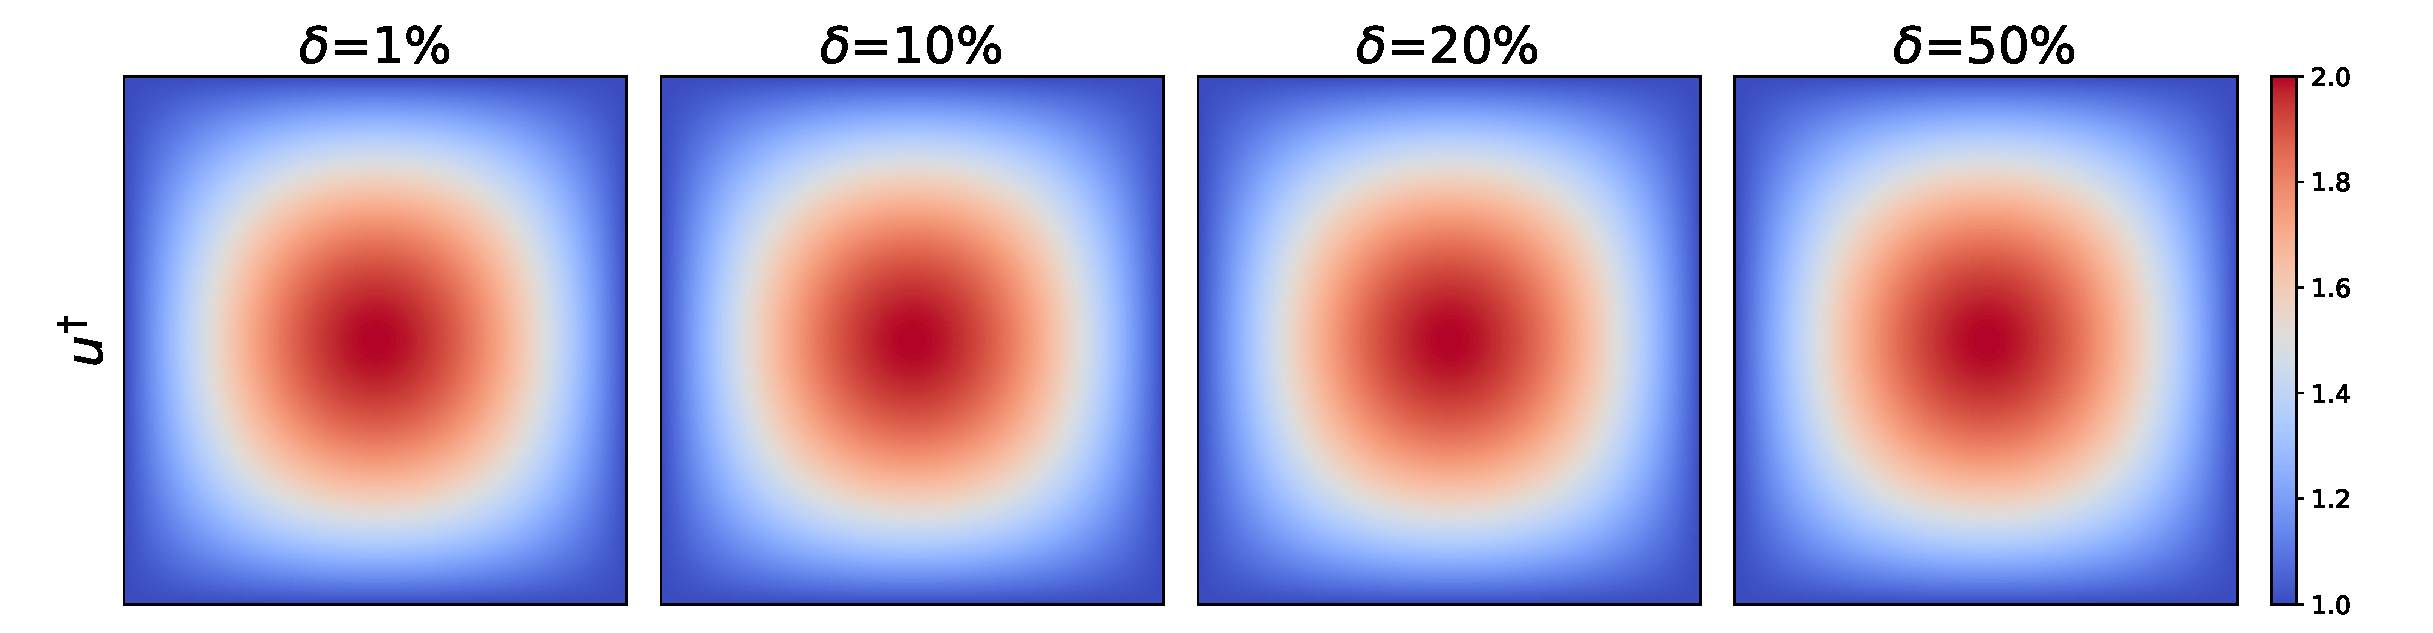
\includegraphics[width=\textwidth]{figures3/discontinuous_udag.eps}\par
% 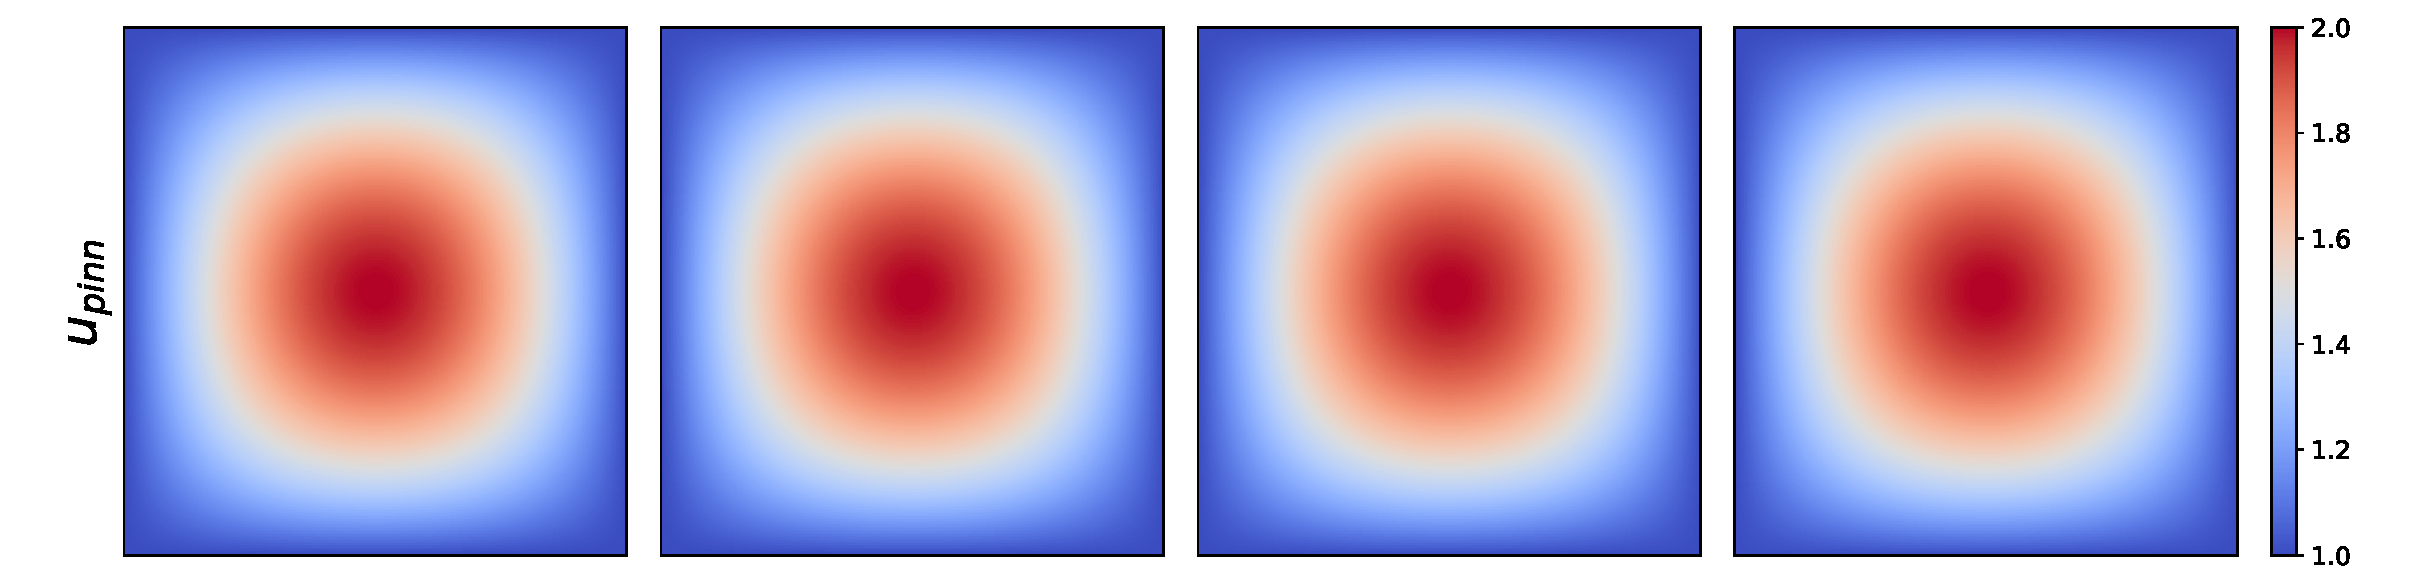
\includegraphics[width=\textwidth]{figures3/discontinuous_unn.eps}\par
% 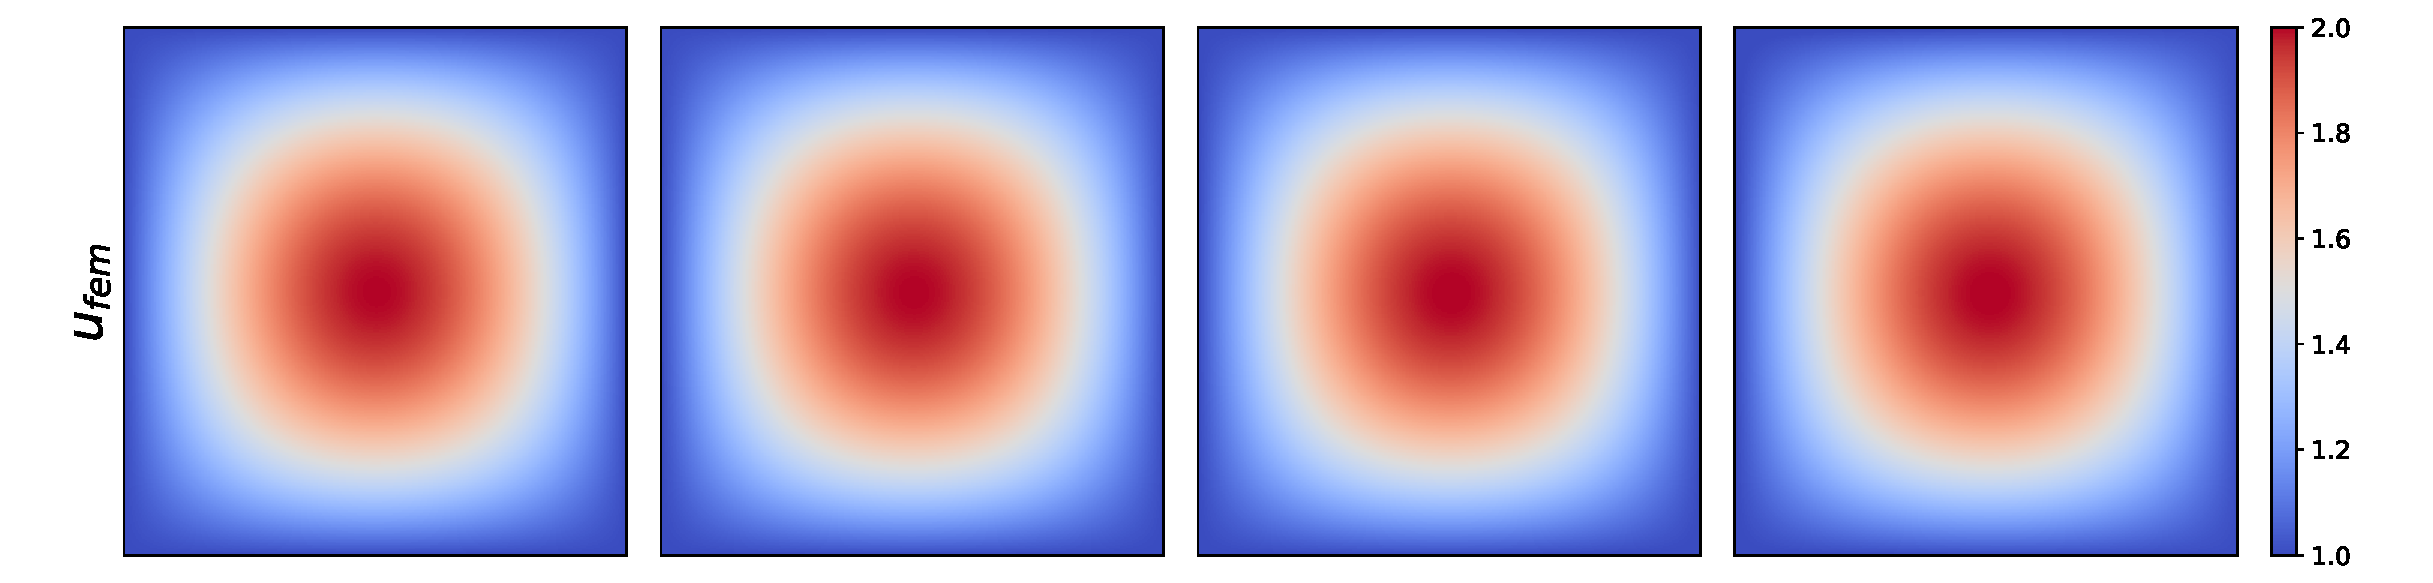
\includegraphics[width=\textwidth]{figures3/discontinuous_ufem.eps}\par
% 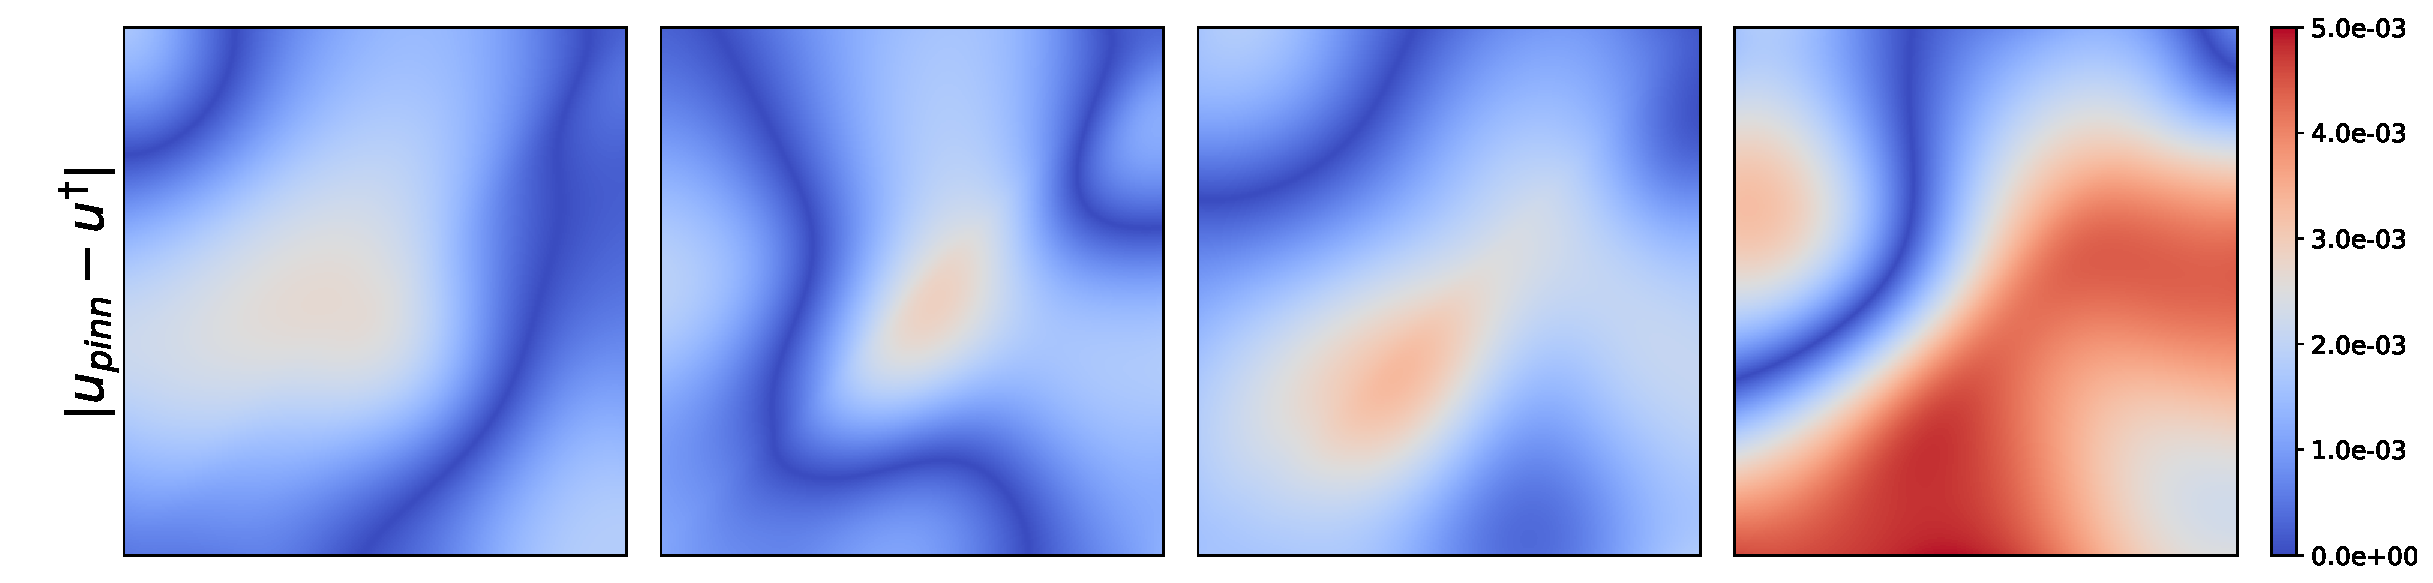
\includegraphics[width=\textwidth]{figures3/discontinuous_unn_err.eps}\par
% 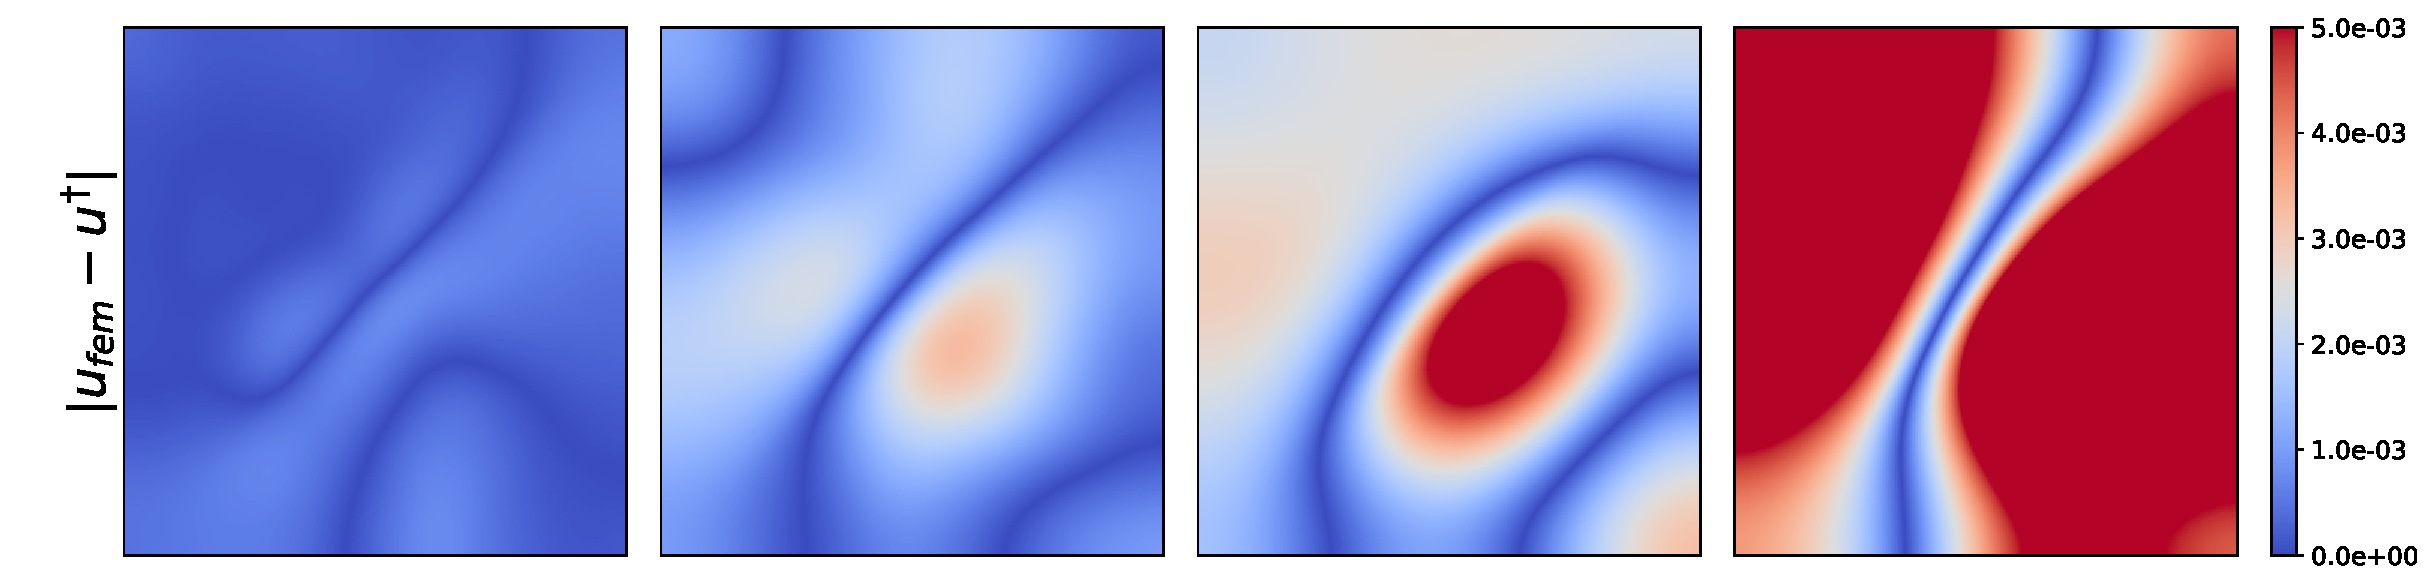
\includegraphics[width=\textwidth]{figures3/discontinuous_ufem_err.eps}
% \caption{从上到下依次为：例 \ref{example:discontinuous} 中的真实解 $u^{\dagger}$，Tikhonov-PINNs 恢复的解 $u_{\text{pinn}}$，逐点绝对误差 $|u^{\dagger}-u_{\text{pinn}}|$，FEM 恢复的解 $u_{\text{fem}}$，以及逐点绝对误差 $|u^{\dagger}-u_{\text{fem}}|$。我们绘制了在不同噪声水平下的结果。}
% \label{fig:example:discontinuous:u}
% \end{figure}

% \begin{figure}[htbp]
% \centering
% \setlength{\abovecaptionskip}{10pt}
% 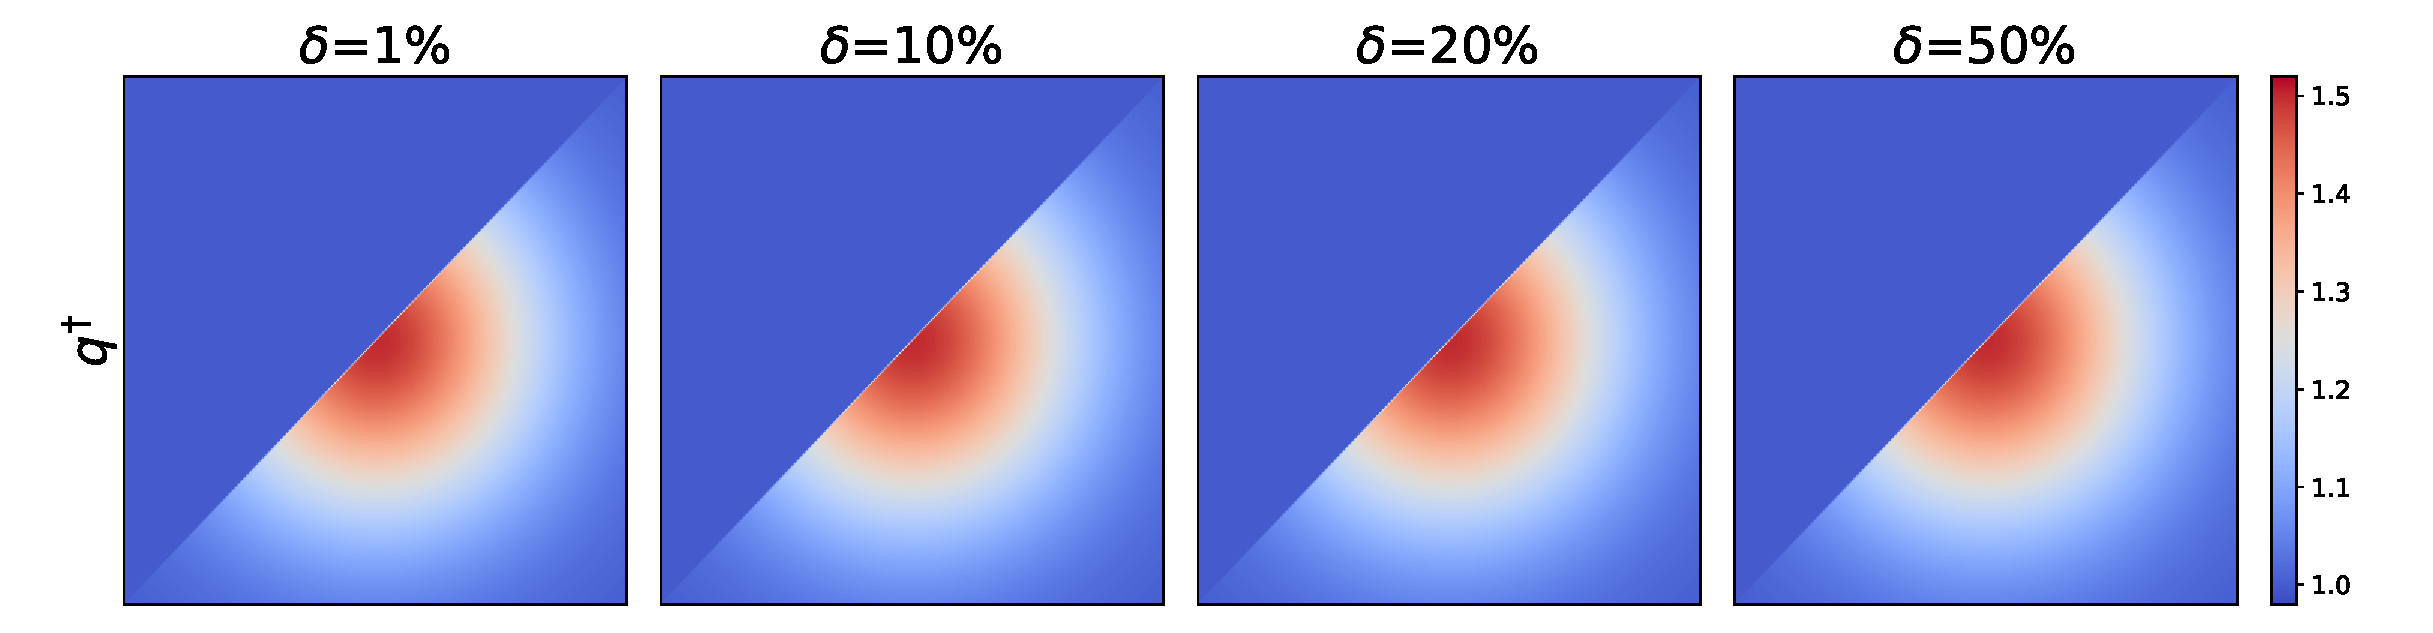
\includegraphics[width=\textwidth]{figures3/discontinuous_qdag.eps}\par
% 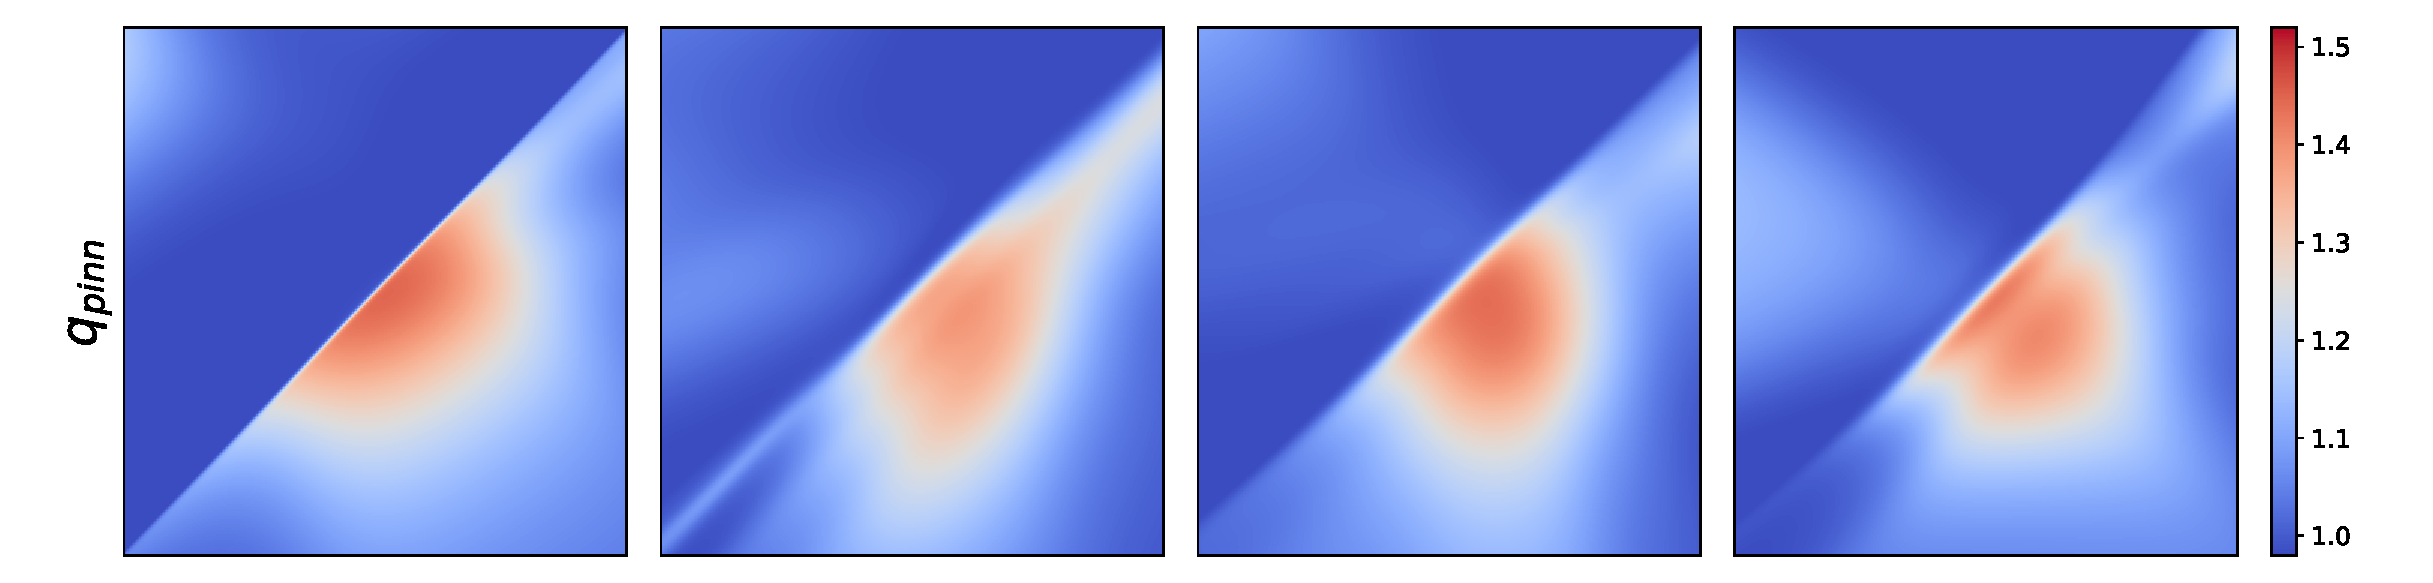
\includegraphics[width=\textwidth]{figures3/discontinuous_qnn.eps}\par
% 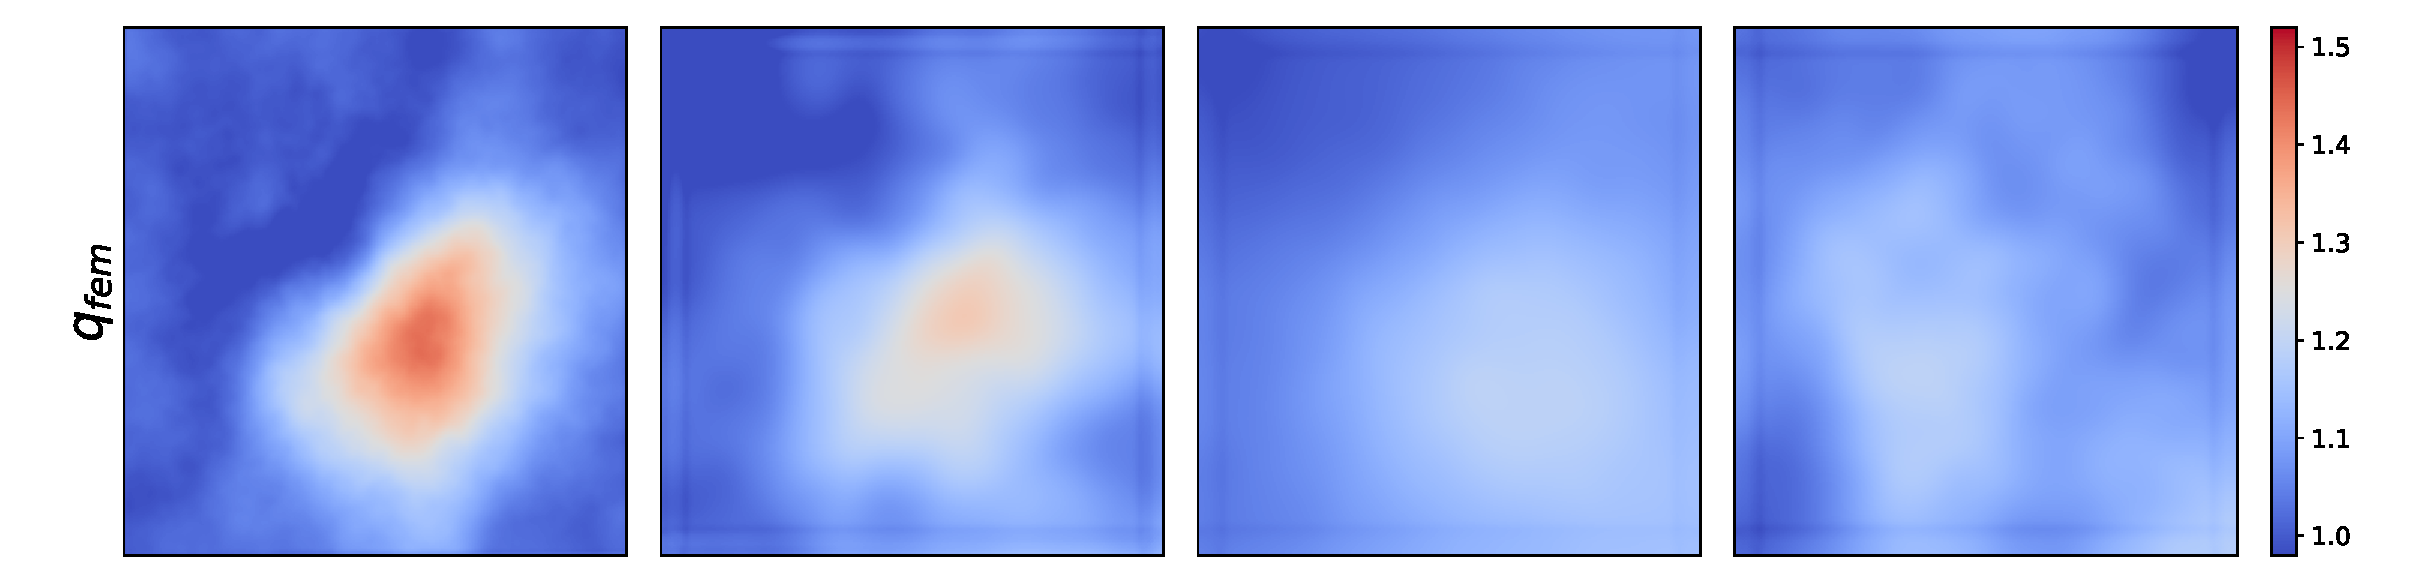
\includegraphics[width=\textwidth]{figures3/discontinuous_q_fem.eps}\par
% 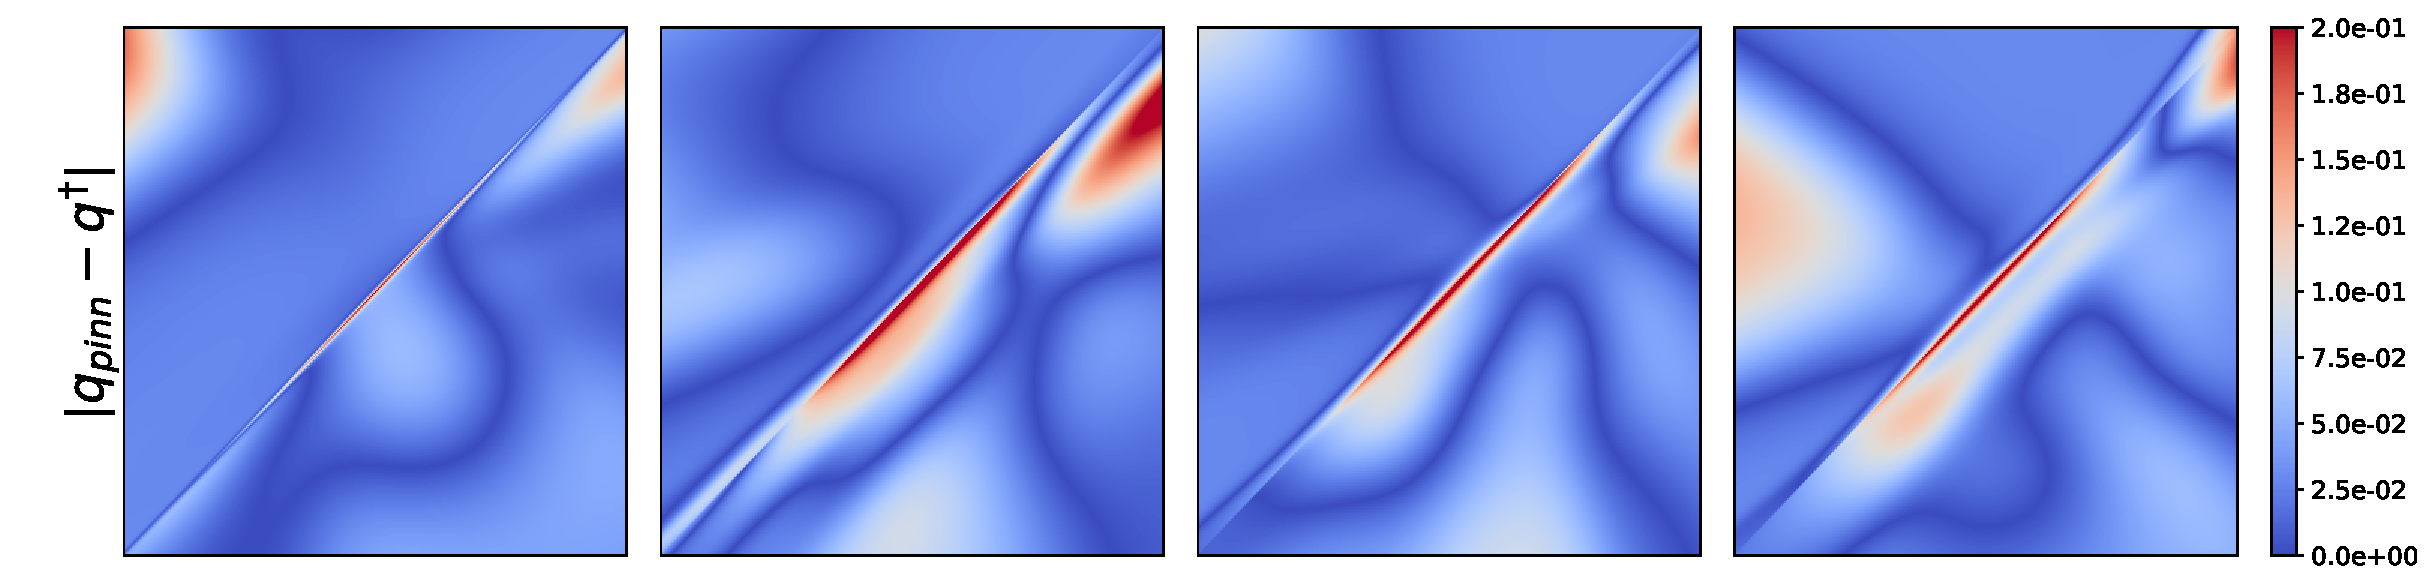
\includegraphics[width=\textwidth]{figures3/discontinuous_qnn_err.eps}\par
% 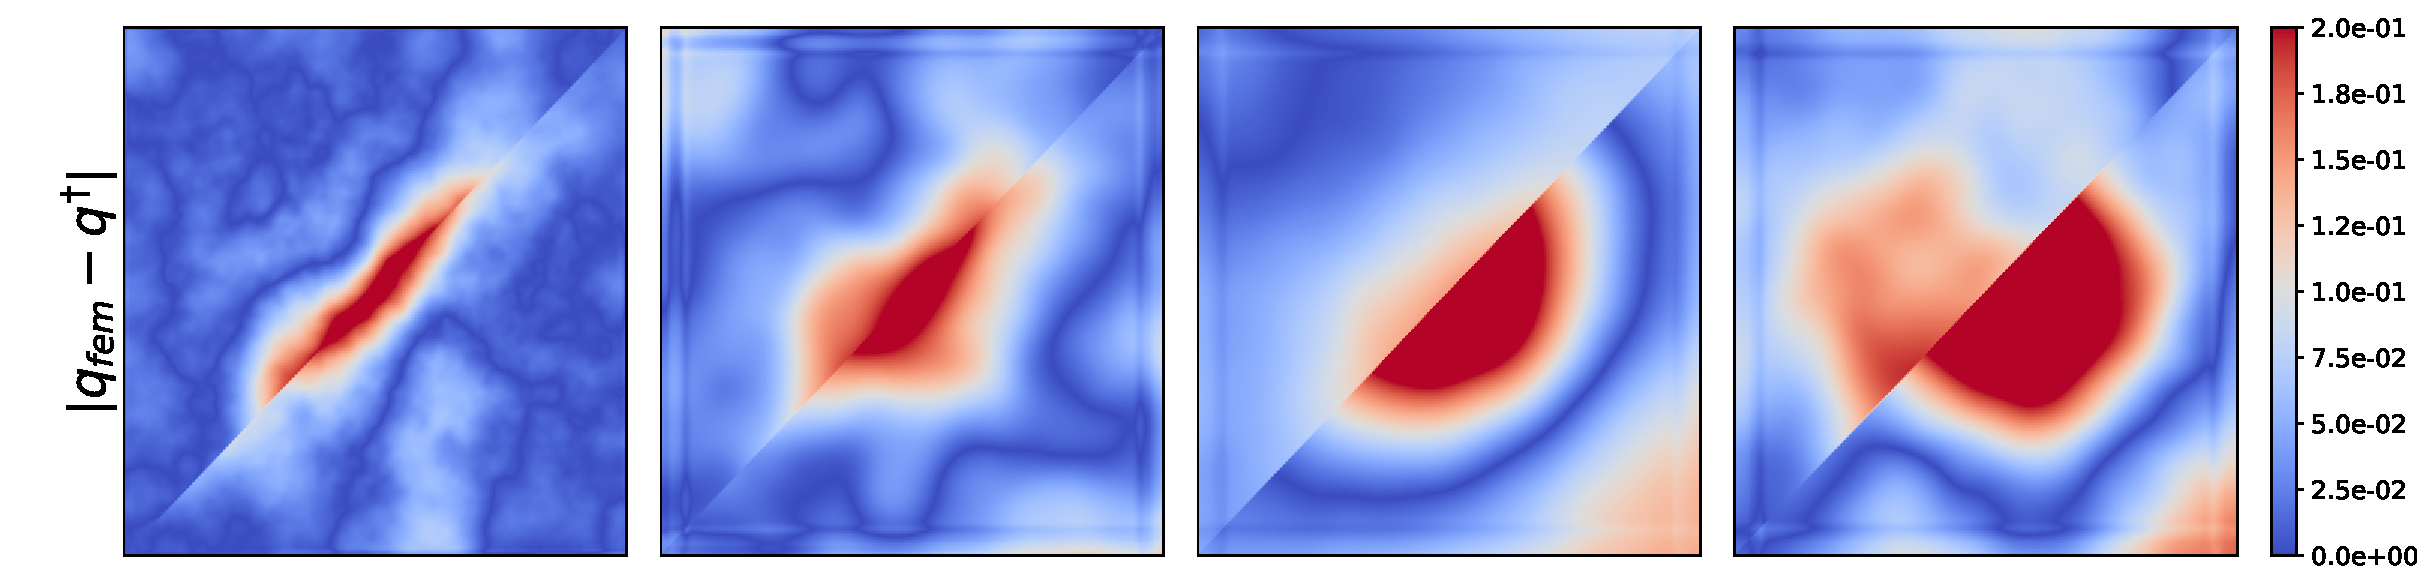
\includegraphics[width=\textwidth]{figures3/discontinuous_qfem_err.eps}
% \caption{从上到下依次为：例 \ref{example:discontinuous} 中的真实势函数 $q^{\dagger}$，Tikhonov-PINNs 恢复的势函数 $q_{\text{pinn}}$，逐点绝对误差 $|q^{\dagger}-q_{\text{pinn}}|$，FEM 恢复的势函数 $q_{\text{fem}}$，以及逐点绝对误差 $|q^{\dagger}-q_{\text{fem}}|$。我们绘制了在不同噪声水平下的结果。}
% \label{fig:example:discontinuous}
% \end{figure}

% 根据构造，势函数 $q$ 沿对角线 $x=y$ 呈现不连续性，这进一步加剧了反问题的不适定性。如图~\ref{fig:example:discontinuous:u} 和图~\ref{fig:example:discontinuous} 所示，Tikhonov-PINNs 能够在所有噪声水平下捕捉到这种不连续性。相比之下，有限元方法无法识别不连续区域，仅能在 1\% 的噪声水平下粗略定位高势区域。如表 \ref{tab:discontinuous} 所示，Tikhonov-PINNs 在所有噪声水平下对 $q$ 的相对误差均达到 $\calO(10^{-2})$ 左右，通常比有限元方法优越一个数量级。

% 还应注意，在上述实验中，当 $\lambda$ 非零时，Tikhonov-PINNs 通常能获得最优解（参见表 \ref{tab:discontinuous}）。这一观察结果部分说明了损失函数中的 Tikhonov 正则化对于提升标准 PINNs 方法的性能至关重要。

% \subsection{高维问题}
% 由于其无网格的特性，基于神经网络的方法可以很容易地扩展到高维问题，并在一定程度上缓解维数灾难。在本小节中，依照 \cite{jin2023conductivity} 中算例 5.4 的设置，我们将 Tikhonov-PINNs 应用于一个五维问题，这是传统有限元方法难以实现的场景。

% \begin{example}\label{example:highdim}
% 令 $\Omega=(0,1)^{5}$ 且 $\alpha\equiv 1$。我们考虑识别如下势函数：
% \begin{equation*}
% \begin{array}{rcl}
% q^{\dagger}(x)&=&1-(x_1-0.5)^2-(x_2-0.5)^2\\
% &{}&+\cos(\pi(x_3+1.5))+\cos(\pi (x_4+1.5))+\cos(\pi (x_5+1.5)),
% \end{array}
% \end{equation*}
% 准确解 $u^{\dagger}$ 为 $u^{\dagger}(x)=\sum_{i=1}^{5}(x_{i}+\frac{1}{3}x_{i}^3)$。
% \end{example}


% \begin{figure}
% \centering
% \setlength{\abovecaptionskip}{10pt}
% 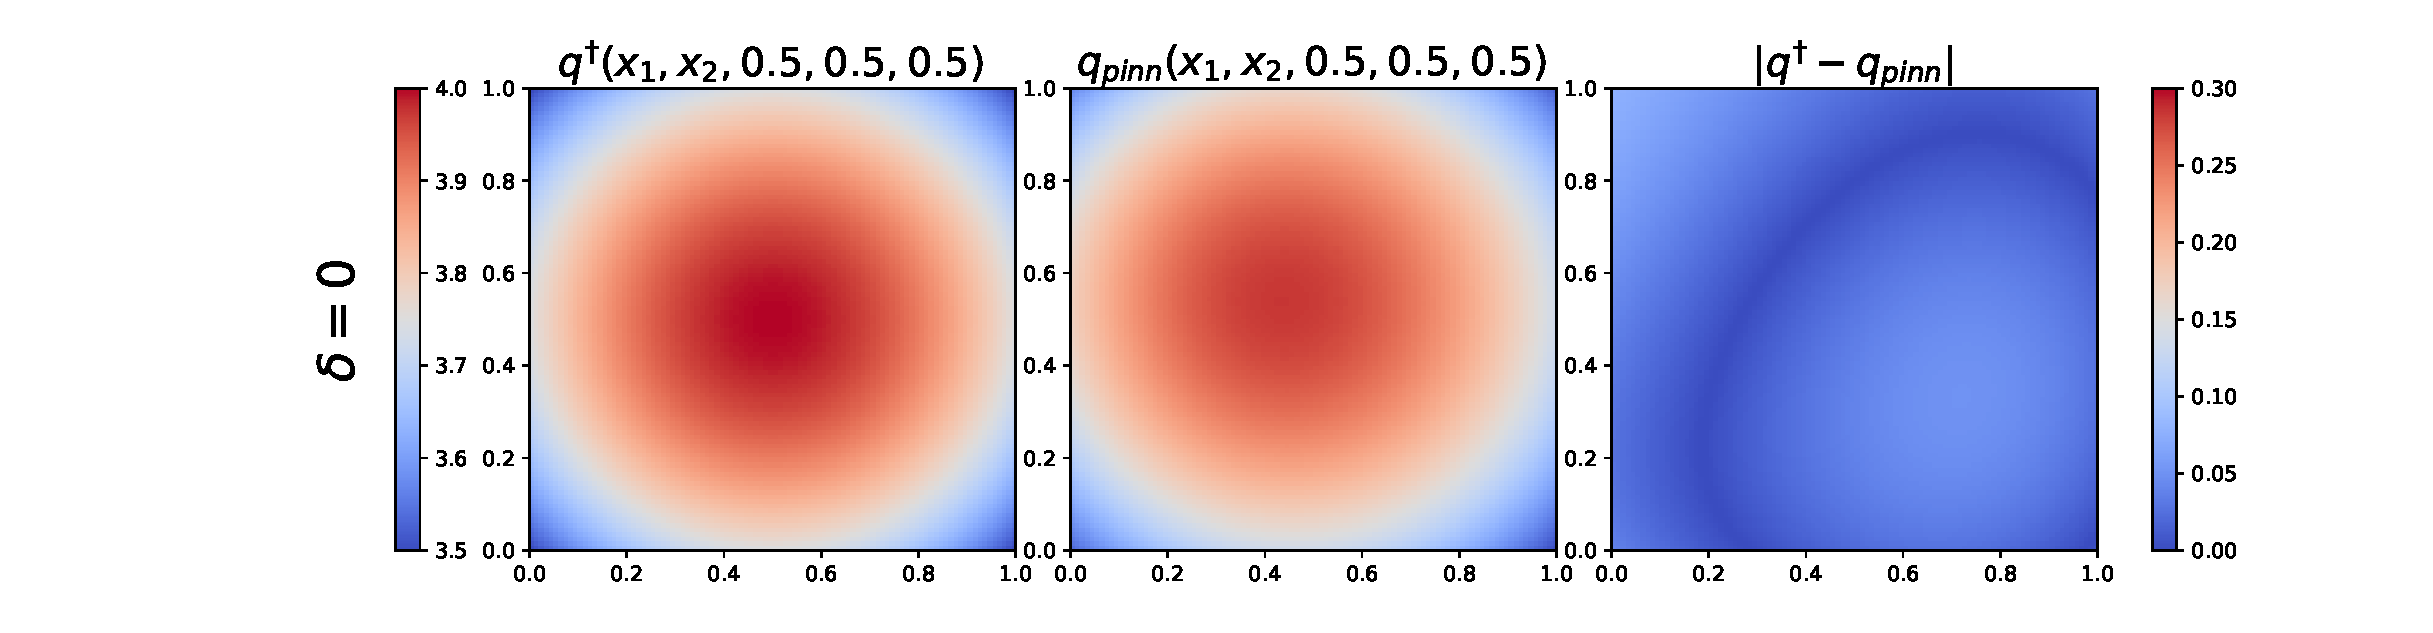
\includegraphics[width=\textwidth]{figures3/ex_5_00.eps}\par
% 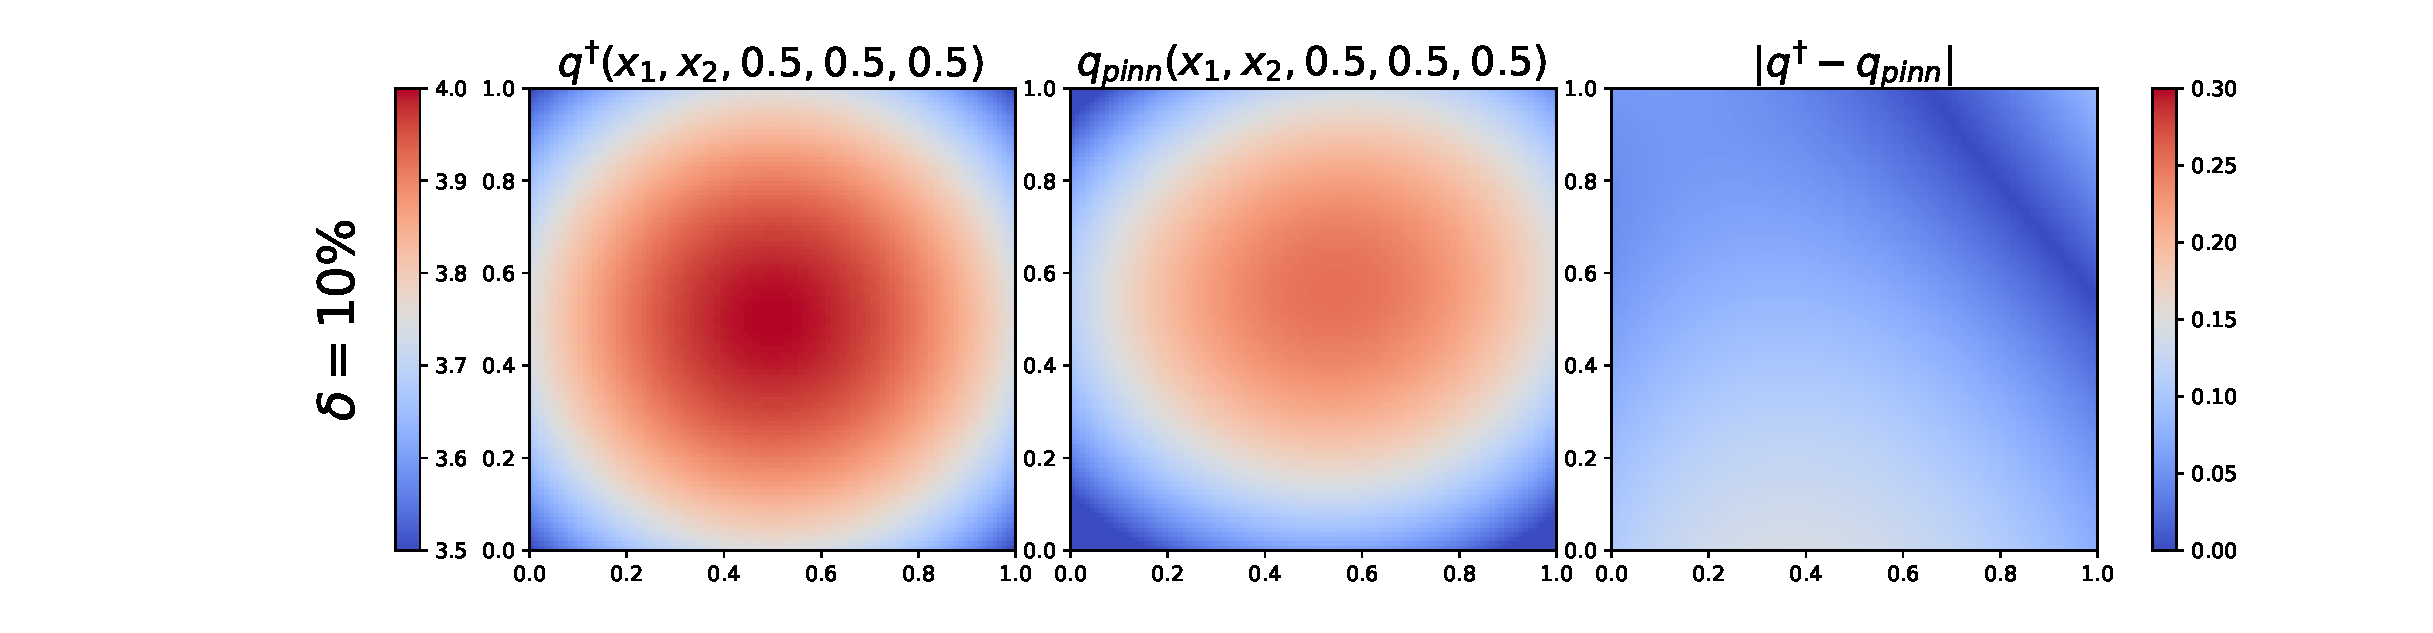
\includegraphics[width=\textwidth]{figures3/ex_5_10.eps}\par
% \caption{算例 \ref{example:highdim} 在切片 $x_3=x_4=x_5=0.5$ 上的真实解与 Tikhonov-PINNs 解。第一行对应 $\delta=0$ 的情况，而第二行展示了 $\delta=10\%$ 的情况。}
% \label{fig:example:highdim}
% \end{figure}

% \begin{table}[hbtp]
% \centering
% \caption{算例 \ref{example:highdim} 中恢复的势 $\hat{q}$ 和解 $\hat{u}$ 的相对 $L^{2}$ 误差。}
% \begin{tabular}{crrrr}
% \hline
% 正则化参数 $\lambda$ & $1.0\times 10^{-7}$ & $1.0\times 10^{-8}$ & $1.0\times 10^{-9}$ & $0$ \\
% \hline
% $\text{err}(u_{\text{pinn}})(\delta=0)$ & $1.09\times 10^{-3}$ & $1.14\times 10^{-3}$ & $1.05\times 10^{-3}$ & $1.39\times 10^{-3}$ \\
% $\text{err}(q_{\text{pinn}})(\delta=0)$ & $3.14\times 10^{-2}$ & $3.08\times 10^{-2}$ & \textbf{3.07$\times$ 10$^{-2}$} & $3.09\times 10^{-2}$  \\
% $\text{err}(u_{\text{pinn}})(\delta=10\%)$ & $4.21\times 10^{-3}$ & $4.19\times 10^{-3}$ & $4.19\times 10^{-3}$ & $4.18\times 10^{-3}$  \\
% $\text{err}(q_{\text{pinn}})(\delta=10\%)$ & $4.33\times 10^{-2}$ & $4.25\times 10^{-2}$ & \textbf{4.24$\times$ 10$^{-2}$} & \textbf{4.24$\times$ 10$^{-2}$}  \\
% \hline
% \end{tabular}
% \label{tab:highdim}
% \end{table}

% 在实验中，我们使用了一个包含 4 个隐藏层且宽度为 26 的神经网络。我们在内部采样了 60,000 个点，在边界上采样了 60,000 个点。模型使用 Adam 优化器训练了 50,000 次迭代，学习率为 $10^{-4}$, 权重衰减系数为 $10^{-9}$。

% 算法误差结果总结在表 \ref{tab:highdim} 中。此外，我们对 $x_{3}=x_{4}=x_{5}=0.5$ 处的切片进行了可视化，如图~\ref{fig:example:highdim} 所示。结果表明，Tikhonov-PINNs 在解决这一五维问题时依然有效，能够准确逼近解和潜在的势函数。

% \subsection{缓解半收敛现象}\label{sec:semi_converge}
% 众所周知，半收敛现象经常出现在不适定反问题中 \cite{engl1996regularization}。在优化的早期阶段，迭代解逐渐逼近真实解。然而，随着迭代的进行，数据噪声的放大导致解偏离真实解，从而导致误差增加。正如 Figure~\ref{fig:err_q} 所示，对于算例 5.3，基于有限元的方法的重构误差最初下降，但随后显著上升，特别是在高噪声水平下。相比之下，Tikhonov-PINNs 有效地缓解了这一问题。我们方法的误差随着迭代次数的增加平滑且持续地下降，没有表现出明显的上升。半收敛的存在使得必须使用早停法来获得最优解，这降低了方法的鲁棒性并限制了可达到的精度。相比之下，Tikhonov-PINNs 固有的优势使其对噪声不那么敏感，允许更多的迭代，最终产生更准确的重构结果。

% 此外，我们也可以使用算例 5.3 来比较计算成本。在求解算例 5.3 的单次迭代中，Tikhonov-PINNs 平均需要 1.91 秒，而基于 FEM 的方法需要 2.04 秒。如图 10 所示，经过 120 次迭代（229.2 秒）后，Tikhonov-PINNs 在约 $10^6$ 个采样点下达到了约 $O(10^{-2})$ 的精度。相比之下，基于 FEM 的方法进行 120 次迭代需要 244.8 秒，达到的精度为 $O(10^{-1})$。这些结果凸显了 Tikhonov-PINNs 在精度和计算效率方面的明显优势，特别是对于不连续问题。

% \begin{figure}[htbp]
%    \centering
%    \setlength{\abovecaptionskip}{10pt}
%    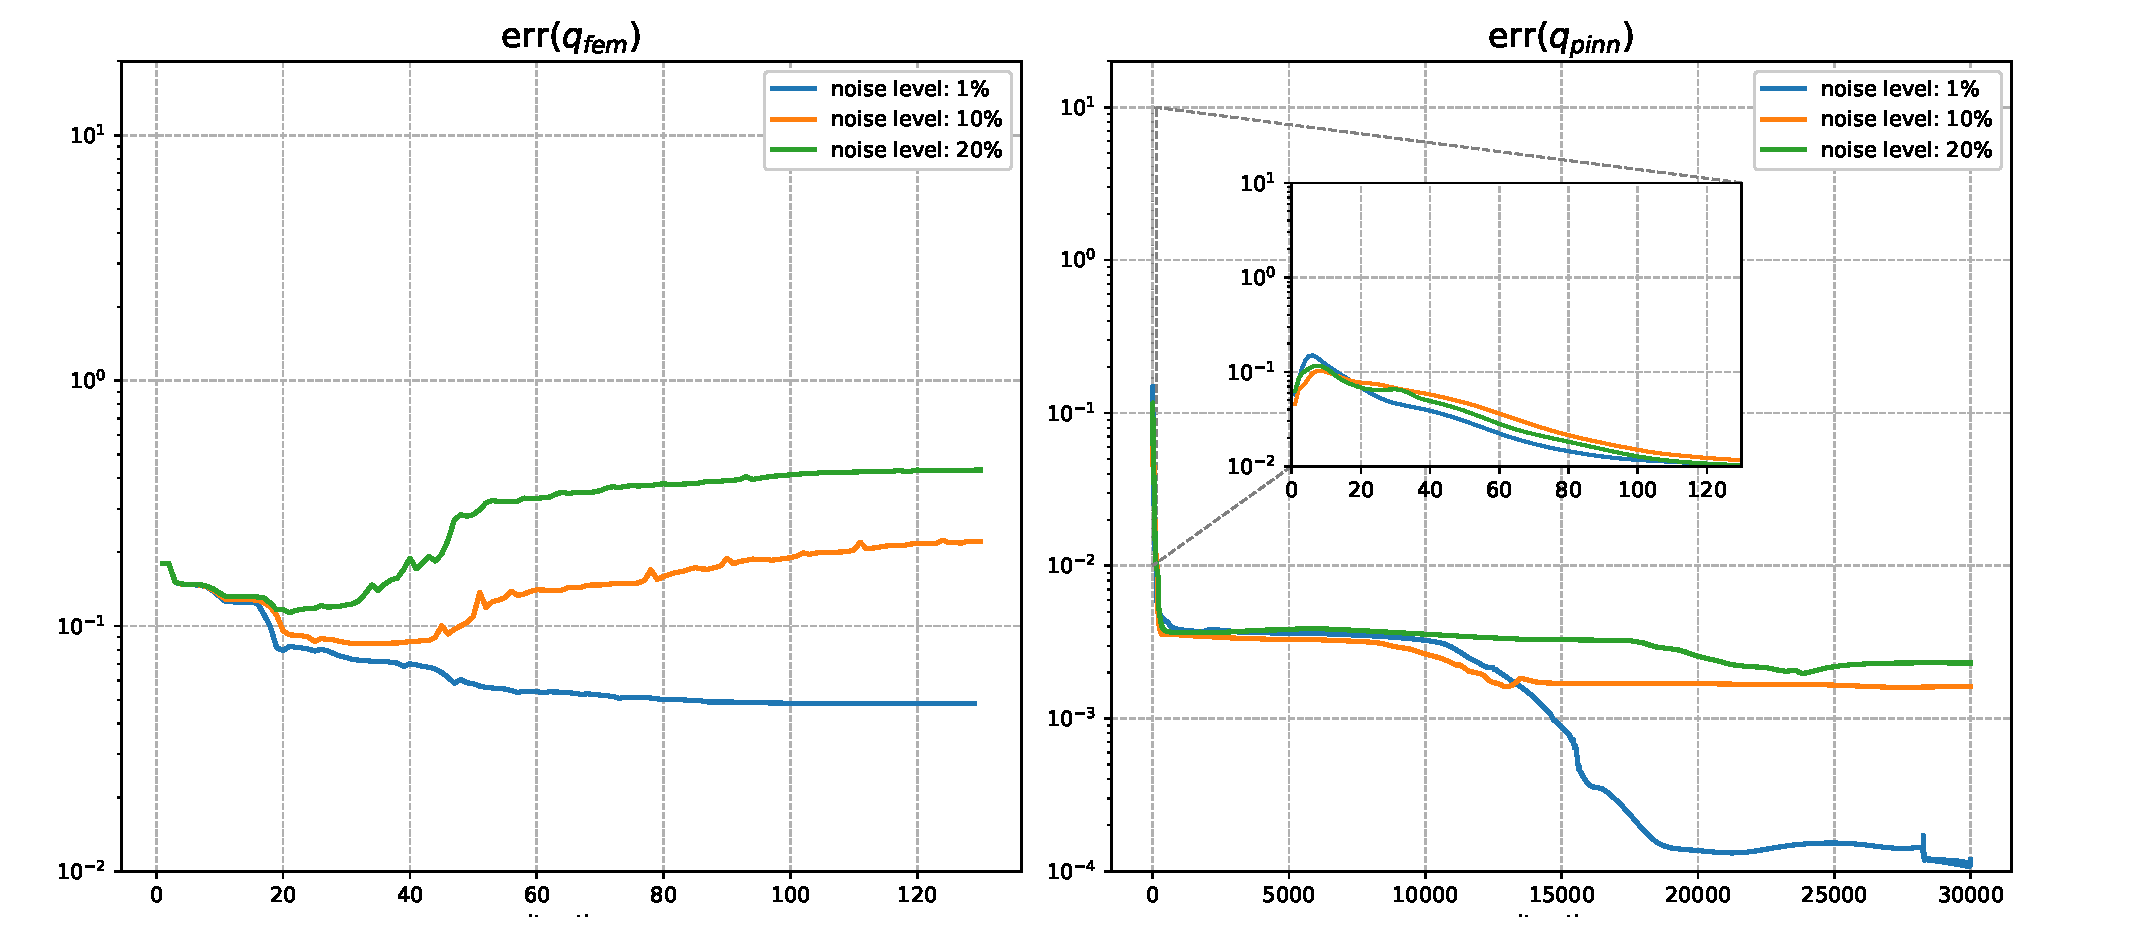
\includegraphics[width=\textwidth]{figures3/err_q.eps}
%    \caption{算例~\ref{example:nonsmooth} 中重构势函数 $q$ 的相对 $L^{2}$ 误差随迭代次数变化的曲线。左列显示了有限元方法获得的结果，而右列显示了 Tikhonov-PINNs 获得的结果。}
%    \label{fig:err_q}
% \end{figure}





\section{理论结果的证明}\label{sec:proof}
\subsection{稳定性的证明}\label{sec:lemma4}
在本小节中，我们将证明定理~\ref{th:potential:stability}，重述如下：

\begin{theorem}[稳定性估计]
在 Eq.\eqref{eq:pde:potential} 和 \eqref{eq:measurement} 的模型下。令 $(q^{\dagger},u^{\dagger})$ 满足 Eq.\eqref{eq:pde:potential}。假设假设 \ref{ass:potential:qudaggerreg} 成立，那么对于每一对满足 $q\in H^{2}(\Omega)$ 的 $(q,u)$，有
\begin{equation*}
\|(q-q^{\dagger})u^{\dagger}\|_{L^{2}(\Omega)}\leq C(1+\lambda^{-1/4}\calL_{\lambda}^{1/4}(q,u))(\calL_{\lambda}^{1/4}(q,u)+\delta^{1/2}),
\end{equation*}
其中 $C$ 是一个依赖于 $d$, $\Omega$, $\alpha$, $\overline{q}$, $\|q^{\dagger}\|_{W^{2,\infty}(\Omega)}$ 和 $\|u^{\dagger}\|_{W^{2,\infty}(\Omega)}$ 的正常数。
\end{theorem}

\begin{proof}
对于每个函数 $\psi\in H^{2}(\Omega)$，有
\begin{align*}
&((q^{\dagger}-q)u^{\dagger},\psi)_{L^{2}(\Omega)} \\
&=(-\nabla\cdot(\alpha\nabla u^{\dagger})_{L^{2}(\Omega)}+q^{\dagger}u^{\dagger},\psi)_{L^{2}(\Omega)}-(-\nabla\cdot(\alpha\nabla u^{\dagger})+qu^{\dagger},\psi)_{L^{2}(\Omega)} \\
&=(f+\nabla\cdot(\alpha\nabla u)-qu,\psi)_{L^{2}(\Omega)}-(q(u^{\dagger}-u),\psi)_{L^{2}(\Omega)}+(\nabla\cdot(\alpha\nabla(u^{\dagger}-u)),\psi)_{L^{2}(\Omega)} \\
&=(f+\nabla\cdot(\alpha\nabla u)-qu,\psi)_{L^{2}(\Omega)}-(q(u^{\dagger}-u),\psi)_{L^{2}(\Omega)}+(u^{\dagger}-u,\nabla\cdot(\alpha\nabla\psi))_{L^{2}(\Omega)} \\
&\quad-(T(u-u^{\dagger}),\alpha\partial_{\nu}\psi)_{L^{2}(\partial\Omega)}+(\alpha\partial_{\nu}u-g,T\psi)_{L^{2}(\partial\Omega)},
\end{align*}
这里我们使用了格林公式以及 $(q^{\dagger},u^{\dagger})$ 满足 Eq.\eqref{eq:pde:potential} 这一事实。应用柯西-施瓦茨不等式和迹定理 \cite[Theorem 1 in Section 5.5]{evans2010partial}，我们有
\begin{align*}
&((q-q^{\dagger})u^{\dagger},\psi)_{L^{2}(\Omega)} \\
&\leq C\big\{\|f+\nabla\cdot(\alpha\nabla u)-qu\|_{L^{2}(\Omega)}+\|q\|_{L^{\infty}(\Omega)}\|u-u^{\dagger}\|_{L^{2}(\Omega)}+\|u-u^{\dagger}\|_{L^{2}(\Omega)} \\
&\quad+\|T(u-u^{\dagger})\|_{L^{2}(\partial\Omega)}+\|\alpha\partial_{\nu}u-g\|_{L^{2}(\partial\Omega)}\big\}(\|\alpha\|_{C^{1}(\bar\Omega)}\vee1)\|\psi\|_{H^{2}(\Omega)} \\
&\leq C\big\{\|f+\nabla\cdot(\alpha\nabla u)-qu\|_{L^{2}(\Omega)}+\|\alpha\partial_{\nu}u-g\|_{L^{2}(\partial\Omega)}+\|q\|_{L^{\infty}(\Omega)}\|z^{\delta}-u\|_{L^{2}(\Omega)} \\
&\quad+\|Tz^{\delta}-Tu\|_{L^{2}(\partial\Omega)}+(\|q\|_{L^{\infty}(\Omega)}+1)\delta\big\}(\|\alpha\|_{C^{1}(\bar\Omega)}\vee1)\|\psi\|_{H^{2}(\Omega)},
\end{align*}
其中最后一个不等式是由于 Eq.\eqref{eq:measurement}，且 $C$ 是一个仅依赖于 $\Omega$ 的常数。因此，由算术-几何均值不等式（AM-GM inequality）可得
\begin{equation*}
\|(q-q^{\dagger})u^{\dagger}\|_{(H^{2}(\Omega))^{*}}\leq 2C(\|q\|_{L^{\infty}(\Omega)}+1)(\|\alpha\|_{C^{1}(\bar\Omega)}\vee1)\Big\{\calL_{\lambda}^{1/2}(q,u)+\delta\Big\}.
\end{equation*}
最后，利用假设 \ref{ass:potential:qudaggerreg} 可得
\begin{align*}
\|(q-q^{\dagger})u^{\dagger}\|_{L^{2}(\Omega)}&\leq\|(q-q^{\dagger})u^{\dagger}\|_{H^{2}(\Omega)}^{1/2}\|(q-q^{\dagger})u^{\dagger}\|_{(H^{2}(\Omega))^{*}}^{1/2} \\
&\lesssim\|q^{\dagger}\|_{W^{2,\infty}(\Omega)}^{1/2}\|u^{\dagger}\|_{W^{2,\infty}(\Omega)}^{1/2}(1+\|q\|_{H^{2}(\Omega)}^{1/2})\|(q-q^{\dagger})u^{\dagger}\|_{(H^{2}(\Omega))^{*}}^{1/2} \\
&\leq C(1+\lambda^{-1/4}\calL_{\lambda}^{1/4}(q,u))(\calL_{\lambda}^{1/4}(q,u)+\delta^{1/2}),
\end{align*}
证明完毕。
\end{proof}


% \subsection{误差分解}\label{sec:lemma5}
% 本小节致力于建立超额风险（excess risk）的误差分解，将其分离为逼近项和泛化项。这一框架使得我们能够利用函数逼近理论和覆盖数估计来分别界定每一部分。首先，我们给出覆盖数和度量熵的定义如下。

% \begin{definition}[覆盖数与度量熵]
% \label{def:covering}
% 令 \(({\cal X},\|\cdot\|_{{\cal X}})\) 为一个度量空间，且 \({\cal Y}\subseteq{\cal X}\)。令 \(\tau>0\)。若对于任意 \(g\in{\calY}\)，都存在 \(g_{\tau}\in{\calY}_{\tau}\) 使得 \(\|g-g_{\tau}\|_{{\cal X}}\leq\tau\)，则我们称 \({\calY}_{\tau}\) 为 \({\calY}\) 的一个 \(\|\cdot\|_{{\cal X}}\) \(\tau\)-覆盖。此外，
% \begin{equation*}
%   N(\tau,{\calY},{\calX})=\min\left\{|{\calY}_{\tau}|\colon{\calY}_{\tau}\mbox{ 是 }{\calY}\mbox{ 的一个 }\|\cdot\|_{{\cal X}}\;\tau\mbox{-覆盖}\right\}
% \end{equation*}
% 被称为 \({\calY}\) 的 \(\|\cdot\|_{{\cal X}}\) \(\tau\)-覆盖数，而
% \begin{equation*}
%   H(\tau,{\calY},{\cal X})=\log N(\tau,{\calY},{\cal X})
% \end{equation*}
% 被称为 \({\calY}\) 的 \(\|\cdot\|_{{\cal X}}\) \(\tau\)-度量熵。
% \end{definition}

% \begin{lemma}\label{lemma:errdec}
%    假设 $\|q\|_{W^{2,\infty}(\Omega)},\|q^{\dagger}\|_{W^{2,\infty}(\Omega)}\leq B_{\calQ}$ 且 $\|u\|_{W^{2,\infty}(\Omega)},\|u^{\dagger}\|_{W^{2,\infty}(\Omega)}\leq B_{\calU}$。设 Assumption \ref{allcondition} 中的假设 (ii) 成立。令 $\euS=\{\euD_{\calI},\euD_{\calB},\euX_{\calI},\euX_{\calB}\}$。令 $(\hat{q},\hat{u})\in\calQ\times\calU$ 为由 \eqref{eq:erm} 定义的经验风险最小化子，则有
%    \begin{align*}
%    \bbE_{\euS}\big[\calE_{\lambda}(\hat{q},\hat{u})\big]
%    &\lesssim\inf_{\tau>0}\Big\{\Delta_{\calQ}H(\tau,\calQ,W^{2,\infty}(\Omega))+\Delta_{\calU}H(\tau,\calU,W^{2,\infty}(\Omega))+\Delta\tau\Big\} \\
%    &\quad+\inf_{(q,u)\in\calQ\times\calU}\calE_{\lambda}(q,u),
%    \end{align*}
%    其中 $\bbE_{\euS}$ 表示关于随机样本集 $\mathcal{S}$ 取的期望，且
%    \begin{align*}
%    \Delta_{\calQ}&=\Big\{\lambda B_{\calQ}^{2}\frac{|\Omega|}{n_{\calI}}+(B_{\alpha}^{2}B_{\calU}^{2}+B_{\calQ}^{2}B_{\calU}^{2}+B_{f}^{2})\frac{|\Omega|}{n_{\calI}}\Big\}, \\
%    \Delta_{\calU}&=\Big\{(B_{\calU}^{2}+\delta^{2})\Big(\frac{|\Omega|}{m_{\calI}}+\frac{|\partial\Omega|}{m_{\calB}}\Big)+(B_{\alpha}^{2}B_{\calU}^{2}+B_{\calQ}^{2}B_{\calU}^{2}+B_{f}^{2})\frac{|\Omega|}{n_{\calI}}+(B_{\alpha}^{2}B_{\calU}^{2}+B_{g}^{2})\frac{|\partial\Omega|}{n_{\calB}}\Big\}, \\
%    \Delta&=(|\Omega|+|\partial\Omega|)C(B_{\alpha},B_{f},B_{g})\{B_{\calQ}B_{\calU}(B_{\calQ}+B_{\calU})+\delta\}.
%    \end{align*}
% \end{lemma}

% \begin{proof}
% \par 首先，我们分别引入 $\calQ\subseteq W^{2,\infty}(\Omega)$ 和 $\calU\subseteq W^{2,\infty}(\Omega)$ 的 $W^{2,\infty}(\Omega)$ $\tau$-覆盖。令 $\tau>0$，并令 $\calQ_{\tau}$ 为 $\calQ$ 的 $W^{2,\infty}(\Omega)$ $\tau$-覆盖，$\calU_{\tau}$ 为 $\calU$ 的 $W^{2,\infty}(\Omega)$ $\tau$-覆盖，满足
% \begin{equation*}
% |\calU_{\tau}|=N(\tau,\calU,W^{2,\infty}(\Omega))\quad\text{and}\quad|\calQ_{\tau}|=N(\tau,\calQ,W^{2,\infty}(\Omega)).
% \end{equation*}
% 那么对于每个 $u\in\calU$ 和 $q\in\calQ$，存在 $u_{\tau}\in\calU_{\tau}$ 和 $q_{\tau}\in\calQ_{\tau}$ 使得 $\|u-u_{\tau}\|_{W^{2,\infty}(\Omega)}\leq\tau$ 且 $\|q-q_{\tau}\|_{W^{2,\infty}(\Omega)}\leq\tau$。不失一般性，我们假设 $\|q_{\tau}\|_{W^{2,\infty}(\Omega)}\leq B_{\calQ}$ 且 $\|u_{\tau}\|_{W^{2,\infty}(\Omega)}\leq B_{\calU}$。
% \par 由于 $(\hat{q},\hat{u})\in\calQ\times\calU$，对于每个 $\gamma>0$，以下不等式成立
% \begin{equation}\label{eq:proof:errordec:2}
% \bbE_{\euS}\big[\calE_{\lambda}(\hat{q},\hat{u})\big]\leq\bbE_{\euS}\Big[\sup_{(q,u)\in\calQ\times\calU}\calE_{\lambda}(q,u)-(1+\gamma)\what{\calE}_{\lambda}(q,u)\Big]+(1+\gamma)\bbE_{\euS}\big[\what{\calE}_{\lambda}(\hat{q},\hat{u})\big].
% \end{equation}
% 在接下来的证明中，我们要分别估计 Eq.\eqref{eq:proof:errordec:2} 右侧的两项。
% \par\noindent\emph{步骤 1. 估计 Eq.\eqref{eq:proof:errordec:2} 右侧的第一项。}
% \par 由上确界的凸性，Eq.\eqref{eq:proof:errordec:2} 中的第一项可以如下有界
% \begin{align*}
% &\bbE_{\euS}\Big[\sup_{(q,u)\in\calQ\times\calU}\calE_{\lambda}(q,u)-(1+\gamma)\what{\calE_{\lambda}}(q,u)\Big] \\
% &\leq\bbE_{\euD_{\calI}}\Big[\sup_{u\in\calU}\|u-u^{\dagger}\|_{L^{2}(\Omega)}^{2}-(1+\gamma)\|u-u^{\dagger}\|_{L^{2}(\euD_{\calI})}^{2}\Big] \\
% &\quad+\bbE_{\euD_{\calB}}\Big[\sup_{u\in\calU}\|Tu-Tu^{\dagger}\|_{L^{2}(\partial\Omega)}^{2}-(1+\gamma)\|Tu-Tu^{\dagger}\|_{L^{2}(\euD_{\calB})}^{2}\Big] \\
% &\quad+\bbE_{\euX_{\calI}}\Big[\sup_{(q,u)\in\calQ\times\calU}\calI(q,u)-(1+\gamma)\what{\calI}(q,u)\Big]+\bbE_{\euX_{\calB}}\Big[\sup_{u\in\calU}\calB(u)-(1+\gamma)\what{\calB}(u)\Big] \\
% &\quad+\lambda\bbE_{\euX_{\calI}}\Big[\sup_{q\in\calQ}\|q\|_{H^{2}(\Omega)}^{2}-(1+\gamma)\|q\|_{H^{2}(\euX_{\calI})}^{2}\Big].
% \end{align*}
% \par 为方便符号表示，我们定义 $\ell_{\calI}(x;u)=(u(x)-u^{\dagger}(x))^{2}$。那么显然有
% \begin{equation*}
% \|u-u^{\dagger}\|_{L^{2}(\Omega)}^{2}=\bbE_{x}\big[\ell_{\calI}(x;u)\big]\quad\text{and}\quad\|u-u^{\dagger}\|_{L^{2}(\euD_{\calI})}^{2}=\frac{|\Omega|}{m_{\calI}}\sum_{i=1}^{m_{\calI}}\ell_{\calI}(x_{i}^{\calI};u).
% \end{equation*}
% 由于 $\|u\|_{W^{2,\infty}(\Omega)}\leq B_{\calU}$，我们发现对于每个 $x\in\Omega$，有 $0\leq\ell_{\calI}(x;u)\leq4B_{\calU}^{2}$ 且 $\ell_{\calI}^{2}(x;u)\leq4B_{\calU}^{2}\ell_{\calI}(x;u)$。那么通过一些代数运算可得
% \begin{align}
% &\bbE_{\euD_{\calI}}\Big[\sup_{u\in\calU}\|u-u^{\dagger}\|_{L^{2}(\Omega)}^{2}-(1+\gamma)\|u-u^{\dagger}\|_{L^{2}(\euD_{\calI})}^{2}\Big] \nonumber \\
% &=\bbE_{\euD_{\calI}}\Big[\sup_{u\in\calU}\frac{\gamma+2}{2}\bbE_{x}\big[\ell_{\calI}(x;u)\big]-\frac{\gamma}{2}\bbE_{x}\big[\ell_{\calI}(x;u)\big] \nonumber \\
% &\quad\quad\quad\quad-\frac{\gamma+2}{2}\frac{|\Omega|}{m_{\calI}}\sum_{i=1}^{m_{\calI}}\ell_{\calI}(x_{i}^{\calI};u)-\frac{\gamma}{2}\frac{|\Omega|}{m_{\calI}}\sum_{i=1}^{m_{\calI}}\ell_{\calI}(x_{i}^{\calI};u)\Big] \nonumber \\
% &\leq\bbE_{\euD_{\calI}}\Big[\sup_{u\in\calU}\frac{\gamma+2}{2}\bbE_{x}\big[\ell_{\calI}(x;u)\big]-\frac{\gamma}{8B_{\calU}^{2}}\bbE_{x}\big[\ell_{\calI}^{2}(x;u)\big] \nonumber \\
% &\quad\quad\quad\quad-\frac{\gamma+2}{2}\frac{|\Omega|}{m_{\calI}}\sum_{i=1}^{m_{\calI}}\ell_{\calI}(x_{i}^{\calI};u)-\frac{\gamma}{8B_{\calU}^{2}}\frac{|\Omega|}{m_{\calI}}\sum_{i=1}^{m_{\calI}}\ell_{\calI}^{2}(x_{i}^{\calI};u)\Big]. \label{eq:proof:errordec:3}
% \end{align}
% 令 $\tilde{\euD}_{\calI}=\{(\tilde{x}_{i},\tilde{z}_{i}^{\delta})\}_{i=1}^{m_{\calI}}$ 为一个幽灵样本（ghost sample），这意味着 $\{(\tilde{x}_{i},\tilde{z}_{i}^{\delta})\}_{i=1}^{m_{\calI}}$ 是独立地从 Eq.\eqref{eq:measurement} 中抽取，且独立于 $\euD_{\calI}$。假设 $\xi=\{\xi_{i}\}_{i=1}^{m_{\calI}}$ 是一系列独立同分布的 Rademacher 变量，且独立于 $\euD_{\calI}$ 和 $\tilde{\euD}_{\calI}$。那么，利用对称化（symmetrization）技术，可得
% \begin{align}
% &\bbE_{\euD_{\calI}}\Big[\sup_{u\in\calU}\frac{\gamma+2}{2}\bbE_{x}\big[\ell_{\calI}(x;u)\big]-\frac{\gamma}{8B_{\calU}^{2}}\bbE_{x}\big[\ell_{\calI}^{2}(x;u)\big] \nonumber \\
% &\quad\quad\quad\quad-\frac{\gamma+2}{2}\frac{|\Omega|}{m_{\calI}}\sum_{i=1}^{m_{\calI}}\ell_{\calI}(x_{i}^{\calI};u)-\frac{\gamma}{8B_{\calU}^{2}}\frac{|\Omega|}{m_{\calI}}\sum_{i=1}^{m_{\calI}}\ell_{\calI}^{2}(x_{i}^{\calI};u)\Big] \nonumber \\
% &\leq\bbE_{\euD_{\calI}}\Big[\sup_{u\in\calU}\bbE_{\tilde{\euD}_{\calI}}\Big[\frac{\gamma+2}{2}\frac{|\Omega|}{m_{\calI}}\sum_{i=1}^{m_{\calI}}\ell_{\calI}(\tilde{x}_{i}^{\calI};u)-\frac{\gamma}{8B_{\calU}^{2}}\frac{|\Omega|}{m_{\calI}}\sum_{i=1}^{m_{\calI}}\ell_{\calI}^{2}(\tilde{x}_{i}^{\calI};u)\Big] \nonumber \\
% &\quad\quad\quad\quad-\frac{\gamma+2}{2}\frac{|\Omega|}{m_{\calI}}\sum_{i=1}^{m_{\calI}}\ell_{\calI}(x_{i}^{\calI};u)-\frac{\gamma}{8B_{\calU}^{2}}\frac{|\Omega|}{m_{\calI}}\sum_{i=1}^{m_{\calI}}\ell_{\calI}^{2}(x_{i}^{\calI};u)\Big] \nonumber \\
% &\leq\bbE_{\euD_{\calI}}\bbE_{\tilde{\euD}_{\calI}}\Big[\sup_{u\in\calU}\frac{\gamma+2}{2}\frac{|\Omega|}{m_{\calI}}\sum_{i=1}^{m_{\calI}}(\ell_{\calI}(\tilde{x}_{i}^{\calI};u)-\ell_{\calI}(x_{i}^{\calI};u)) \nonumber \\
% &\quad\quad\quad\quad-\frac{\gamma}{8B_{\calU}^{2}}\frac{|\Omega|}{m_{\calI}}\sum_{i=1}^{m_{\calI}}(\ell_{\calI}^{2}(\tilde{x}_{i}^{\calI};u)+\ell_{\calI}^{2}(x_{i}^{\calI};u))\Big] \nonumber \\
% &=\bbE_{\euD_{\calI}}\bbE_{\tilde{\euD}_{\calI}}\bbE_{\xi}\Big[\sup_{u\in\calU}\frac{\gamma+2}{2}\frac{|\Omega|}{m_{\calI}}\sum_{i=1}^{m_{\calI}}\xi_{i}(\ell_{\calI}(\tilde{x}_{i}^{\calI};u)-\ell_{\calI}(x_{i}^{\calI};u)) \nonumber \\
% &\quad\quad\quad\quad-\frac{\gamma}{8B_{\calU}^{2}}\frac{|\Omega|}{m_{\calI}}\sum_{i=1}^{m_{\calI}}(\ell_{\calI}^{2}(\tilde{x}_{i}^{\calI};u)+\ell_{\calI}^{2}(x_{i}^{\calI};u))\Big] \nonumber \\
% &=\bbE_{\euD_{\calI}}\bbE_{\xi}\Big[\sup_{u\in\calU}(\gamma+2)\frac{|\Omega|}{m_{\calI}}\sum_{i=1}^{m_{\calI}}\xi_{i}\ell_{\calI}(x_{i}^{\calI};u)-\frac{\gamma}{4B_{\calU}^{2}}\frac{|\Omega|}{m_{\calI}}\sum_{i=1}^{m_{\calI}}\ell_{\calI}^{2}(x_{i}^{\calI};u)\Big], \label{eq:proof:errordec:4}
% \end{align}
% 其中第二个不等式由 Jensen 不等式成立，且 $\bbE_{\xi}[\cdot]=\bbE[\cdot|\euD_{\calI},\tilde{\euD}_{\calI}]$ 表示关于 $\euD_{\calI}$ 和 $\tilde{\euD}_{\calI}$ 的条件期望。
% \par 我们现在转向估计最后一行的条件期望。回顾 $\calU_{\tau}$ 的定义，对于每个 $u\in\calU$，存在 $u_{\tau}\in\calU_{\tau}$ 使得 $\|u-u_{\tau}\|_{W^{2,\infty}(\Omega)}\leq\tau$，并注意到
% \begin{equation*}
% |\ell_{\calI}(x_{i}^{\calI};u)-\ell_{\calI}(x_{i}^{\calI};u_{\tau})|\leq 4B_{\calU}\tau.
% \end{equation*}
% 因此，我们发现
% \begin{align*}
% &(\gamma+2)\frac{|\Omega|}{m_{\calI}}\sum_{i=1}^{m_{\calI}}\xi_{i}\ell_{\calI}(x_{i}^{\calI};u) \\
% &\leq(\gamma+2)\frac{|\Omega|}{m_{\calI}}\sum_{i=1}^{m_{\calI}}\xi_{i}\ell_{\calI}(x_{i}^{\calI};u_{\tau})+(\gamma+2)\frac{|\Omega|}{m_{\calI}}\sum_{i=1}^{m_{\calI}}|\ell_{\calI}(x_{i}^{\calI};u)-\ell_{\calI}(x_{i}^{\calI};u_{\tau})| \\
% &\leq(\gamma+2)\frac{|\Omega|}{m_{\calI}}\sum_{i=1}^{m_{\calI}}\xi_{i}\ell_{\calI}(x_{i}^{\calI};u_{\tau})+4(\gamma+2)|\Omega|B_{\calU}\tau,
% \end{align*}
% 以及
% \begin{align*}
% &-\frac{\gamma}{4B_{\calU}^{2}}\frac{|\Omega|}{m_{\calI}}\sum_{i=1}^{m_{\calI}}\ell_{\calI}^{2}(x_{i}^{\calI};u) \\
% &\leq-\frac{\gamma}{4B_{\calU}^{2}}\frac{|\Omega|}{m_{\calI}}\sum_{i=1}^{m_{\calI}}\ell_{\calI}^{2}(x_{i}^{\calI};u_{\tau})+2\gamma\frac{|\Omega|}{m_{\calI}}\sum_{i=1}^{m_{\calI}}|\ell_{\calI}(x_{i}^{\calI};u_{\tau})-\ell_{\calI}(x_{i}^{\calI};u)| \\
% &\leq-\frac{\gamma}{4B_{\calU}^{2}}\frac{|\Omega|}{m_{\calI}}\sum_{i=1}^{m_{\calI}}\ell_{\calI}^{2}(x_{i}^{\calI};u_{\tau})+8\gamma|\Omega|B_{\calU}\tau.
% \end{align*}
% 从而
% \begin{equation}\label{eq:proof:errordec:5}
% \begin{aligned}
% &\bbE\Big[\sup_{u\in\calU}(\gamma+2)\frac{|\Omega|}{m_{\calI}}\sum_{i=1}^{m_{\calI}}\xi_{i}\ell_{\calI}(x_{i}^{\calI};u)-\frac{\gamma}{4B_{\calU}^{2}}\frac{|\Omega|}{m_{\calI}}\sum_{i=1}^{m_{\calI}}\ell_{\calI}^{2}(x_{i}^{\calI};u)\Big|\euD_{\calI}\Big] \\
% &\leq\bbE\Big[\sup_{u_{\tau}\in\calU_{\tau}}(\gamma+2)\frac{|\Omega|}{m_{\calI}}\sum_{i=1}^{m_{\calI}}\xi_{i}\ell_{\calI}(x_{i}^{\calI};u_{\tau})-\frac{\gamma}{4B_{\calU}^{2}}\frac{|\Omega|}{m_{\calI}}\sum_{i=1}^{m_{\calI}}\ell_{\calI}^{2}(x_{i}^{\calI};u_{\tau})\Big|\euD_{\calI}\Big] \\
% &\quad+4(3\gamma+2)|\Omega|B_{\calU}\tau.
% \end{aligned}
% \end{equation}
% 由于 $\{\xi_{i}\ell_{\calI}(x_{i}^{\calI};u_{\tau})\}_{i=1}^{m_{\calI}}$ 是以 $\euD_{\calI}$ 为条件的独立随机变量，因此 $\bbE[\xi_{i}\ell_{\calI}(x_{i}^{\calI};u_{\tau})\big|\euD_{\calI}]=0$ 且 $-\ell_{\calI}(x_{i}^{\calI};u_{\tau})\leq\xi_{i}\ell_{\calI}(x_{i}^{\calI};u_{\tau})\leq\ell_{\calI}(x_{i}^{\calI};u_{\tau})$。接着使用 Hoeffding 不等式 \cite[Theorem D.2]{mohri2018foundations} 可得
% \begin{align*}
% &\bbP\Big\{(\gamma+2)\frac{|\Omega|}{m_{\calI}}\sum_{i=1}^{m_{\calI}}\xi_{i}\ell_{\calI}(x_{i}^{\calI};u_{\tau})>t+\frac{\gamma}{4B_{\calU}^{2}}\frac{|\Omega|}{m_{\calI}}\sum_{i=1}^{m_{\calI}}\ell_{\calI}^{2}(x_{i}^{\calI};u_{\tau})\Big|\euD_{\calI}\Big\} \\
% &=\bbP\Big\{\sum_{i=1}^{m_{\calI}}\xi_{i}\ell_{\calI}(x_{i}^{\calI};u_{\tau})>\frac{1}{\gamma+2}\frac{m_{\calI}}{|\Omega|}t+\frac{\gamma}{\gamma+2}\frac{1}{4B_{\calU}^{2}}\sum_{i=1}^{m_{\calI}}\ell_{\calI}^{2}(x_{i}^{\calI};u_{\tau})\Big|\euD_{\calI}\Big\} \\
% &\leq\exp\Big(-\frac{(\frac{\gamma}{\gamma+2}\frac{1}{4B_{\calU}^{2}})^{2}}{2}\frac{(\frac{4B_{\calU}^{2}}{\gamma}\frac{m_{\calI}}{|\Omega|}t+\sum_{i=1}^{m_{\calI}}\ell_{\calI}^{2}(x_{i}^{\calI};u_{\tau}))^{2}}{\sum_{i=1}^{m_{\calI}}\ell_{\calI}^{2}(x_{i}^{\calI};u_{\tau})}\Big) \\
% &\leq\exp\Big(-\frac{\gamma}{(\gamma+2)^{2}}\frac{1}{2B_{\calU}^{2}}\frac{m_{\calI}}{|\Omega|}t\Big),
% \end{align*}
% 其中最后一个不等式源自数值不等式
% \begin{equation*}
% \frac{(a+y)^{2}}{y}\geq\frac{(a+a)^{2}}{a}=4a,\quad y\in\bbR_{+}.
% \end{equation*}
% 对于任意 $T>0$，有
% \begin{align*}
% &\bbE\Big[\sup_{u_{\tau}\in\calU_{\tau}}(\gamma+2)\frac{|\Omega|}{m_{\calI}}\sum_{i=1}^{m_{\calI}}\xi_{i}\ell_{\calI}(x_{i}^{\calI};u_{\tau})-\frac{\gamma}{4B_{\calU}^{2}}\frac{|\Omega|}{m_{\calI}}\sum_{i=1}^{m_{\calI}}\ell_{\calI}^{2}(x_{i}^{\calI};u_{\tau})\Big|\euD_{\calI}\Big] \\
% &=\int_{0}^{\infty}\bbP\Big\{\sup_{u_{\tau}\in\calU_{\tau}}(\gamma+2)\frac{|\Omega|}{m_{\calI}}\sum_{i=1}^{m_{\calI}}\xi_{i}\ell_{\calI}(x_{i}^{\calI};u_{\tau})-\frac{\gamma}{4B_{\calU}^{2}}\frac{|\Omega|}{m_{\calI}}\sum_{i=1}^{m_{\calI}}\ell_{\calI}^{2}(x_{i}^{\calI};u_{\tau})>t\Big|\euD_{\calI}\Big\}dt \\
% &\leq T+\frac{(\gamma+2)^{2}}{\gamma}2B_{\calU}^{2}\frac{|\Omega|}{m_{\calI}}|\calU_{\tau}|\exp\Big(-\frac{\gamma}{(\gamma+2)^{2}}\frac{1}{2B_{\calU}^{2}}\frac{m_{\calI}}{|\Omega|}T\Big).
% \end{align*}
% 将
% $$T=\frac{(\gamma+2)^{2}}{\gamma}2B_{\calU}^{2}\frac{|\Omega|}{m_{\calI}}\log|\calU_{\tau}|$$
% 代入上述不等式，并结合 Eq.\eqref{eq:proof:errordec:3}、Eq.\eqref{eq:proof:errordec:4} 和 Eq.\eqref{eq:proof:errordec:5}，我们得到
% \begin{align}
% &\bbE_{\euD_{\calI}}\bbE_{\xi}\Big[\sup_{u\in\calU}(\gamma+2)\frac{|\Omega|}{m_{\calI}}\sum_{i=1}^{m_{\calI}}\xi_{i}\ell_{\calI}(x_{i}^{\calI};u)-\frac{\gamma}{4B_{\calU}^{2}}\frac{|\Omega|}{m_{\calI}}\sum_{i=1}^{m_{\calI}}\ell_{\calI}^{2}(x_{i}^{\calI};u)\Big] \nonumber \\
% &\leq2(\gamma+2)^{2}\gamma^{-1}|\Omega|B_{\calU}^{2}m_{\calI}^{-1}(1+\log|\calU_{\tau}|)+2(3\gamma+2)|\Omega|B_{\calU}\tau.\label{eq:proof:errordec:6}
% \end{align}


% 类似地，我们定义 $\ell_{\calB}(x;u)=(Tu(x)-Tu^{\dagger}(x))^{2}$，且下列不等式成立
% \begin{align}
% &\bbE_{\euD_{\calB}}\Big[\sup_{u\in\calU}\|Tu-Tu^{\dagger}\|_{L^{2}(\partial\Omega)}^{2}-(1+\gamma)\|Tu-Tu^{\dagger}\|_{L^{2}(\euD_{\calB})}^{2}\Big] \nonumber \\
% &\leq\bbE_{\euD_{\calB}}\bbE_{\xi}\Big[\sup_{u\in\calU}(\gamma+2)\frac{|\partial\Omega|}{m_{\calB}}\sum_{i=1}^{m_{\calB}}\xi_{i}\ell_{\calB}(x_{i}^{\calB};u)-\frac{\gamma}{4B_{\calU}^{2}}\frac{|\partial\Omega|}{m_{\calB}}\sum_{i=1}^{m_{\calB}}\ell_{\calB}^{2}(x_{i}^{\calB};u)\Big] \nonumber \\
% &\leq2(\gamma+2)^{2}\gamma^{-1}|\partial\Omega|B_{\calU}^{2}m_{\calB}^{-1}(1+\log|\calU_{\tau}|)+2(3\gamma+2)|\partial\Omega|B_{\calU}\tau.\label{eq:proof:errordec:7}
% \end{align}
% \par 定义 $p_{\calI}(x;q,u)=(\nabla\cdot(\alpha(x)\nabla u(x))-q(x)u(x)+f(x))^{2}$，并注意到
% \begin{align*}
% &0\leq p_{\calI}(x_{j}^{\calI};q,u)\leq4B_{\alpha}^{2}B_{\calU}^{2}+4B_{\calQ}^{2}B_{\calU}^{2}+4B_{f}^{2}=:B_{p,\calI}^{2}, \\
% &|p_{\calI}(x_{j}^{\calI};q,u)-p_{\calI}(x_{j}^{\calI};q_{\tau},u_{\tau})| \\
% &\leq(2B_{\alpha}B_{\calU}+2B_{\calQ}B_{\calU}+2B_{f})(B_{\alpha}+B_{\calQ}+B_{\calU})\tau=:L_{p,\calI}\tau.
% \end{align*}
% 类似于 Eq.\eqref{eq:proof:errordec:3} 和 Eq.\eqref{eq:proof:errordec:4} 的证明，下列不等式成立
% \begin{align*}
% &\bbE_{\euX_{\calI}}\Big[\sup_{(q,u)\in\calQ\times\calU}\calI(q,u)-(1+\gamma)\what{\calI}(q,u)\Big] \\
% &\leq\bbE_{\euX_{\calI}}\bbE_{\xi}\Big[\sup_{(q,u)\in\calQ\times\calU}(\gamma+2)\frac{|\Omega|}{n_{\calI}}\sum_{j=1}^{n_{\calI}}\xi_{j}p_{\calI}(x_{j}^{\calI};q,u)-\frac{\gamma}{B_{p,\calI}^{2}}\frac{|\Omega|}{n_{\calI}}\sum_{j=1}^{n_{\calI}}p_{\calI}^{2}(x_{j}^{\calI};q,u)\Big],
% \end{align*}
% 其中 $\xi=\{\xi_{j}\}_{j=1}^{n_{\calI}}$ 是独立于 $\euX_{\calI}$ 的独立同分布 (i.i.d.) Rademacher 变量序列。回顾 $\tau$-覆盖 $\calQ_{\tau}$ 和 $\calU_{\tau}$，对于任意 $(q,u)\in\calQ\times\calU$，存在 $(q_{\tau},u_{\tau})\in\calQ_{\tau}\times\calU_{\tau}$ 使得
% \begin{align*}
% (\gamma+2)\frac{|\Omega|}{n_{\calI}}\sum_{j=1}^{n_{\calI}}\xi_{j}p_{\calI}(x_{j}^{\calI};q,u)&\leq(\gamma+2)\frac{|\Omega|}{n_{\calI}}\sum_{j=1}^{n_{\calI}}\xi_{j}p_{\calI}(x_{j}^{\calI};q_{\tau},u_{\tau})+(\gamma+2)|\Omega|L_{p,\calI}\tau, \\
% -\frac{\gamma}{B_{p,\calI}^{2}}\frac{|\Omega|}{n_{\calI}}\sum_{j=1}^{n_{\calI}}p_{\calI}^{2}(x_{j}^{\calI};q,u)&\leq-\frac{\gamma}{B_{p,\calI}^{2}}\frac{|\Omega|}{n_{\calI}}\sum_{j=1}^{n_{\calI}}p_{\calI}^{2}(x_{j}^{\calI};q_{\tau},u_{\tau})+2\gamma|\Omega|L_{p,\calI}\tau.
% \end{align*}
% 从而，
% \begin{align*}
% &\bbE\Big[\sup_{(q,u)\in\calQ\times\calU}(\gamma+2)\frac{|\Omega|}{n_{\calI}}\sum_{j=1}^{n_{\calI}}\xi_{j}p_{\calI}(x_{j}^{\calI};q,u)-\frac{\gamma}{B_{p,\calI}^{2}}\frac{|\Omega|}{n_{\calI}}\sum_{j=1}^{n_{\calI}}p_{\calI}^{2}(x_{j}^{\calI};q,u)\Big|\euX_{\calI}\Big] \\
% &\leq\bbE\Big[\sup_{(q_{\tau},u_{\tau})\in\calQ_{\tau}\times\calU_{\tau}}(\gamma+2)\frac{|\Omega|}{n_{\calI}}\sum_{j=1}^{n_{\calI}}\xi_{j}p_{\calI}(x_{j}^{\calI};q_{\tau},u_{\tau})-\frac{\gamma}{B_{p,\calI}^{2}}\frac{|\Omega|}{n_{\calI}}\sum_{j=1}^{n_{\calI}}p_{\calI}^{2}(x_{j}^{\calI};q_{\tau},u_{\tau})\Big|\euX_{\calI}\Big] \\
% &\quad+(3\gamma+2)|\Omega|L_{p,\calI}\tau.
% \end{align*}
% 在估计条件期望之前，我们首先通过下列不等式对尾概率进行控制
% \begin{align*}
% &\bbP\Big\{(\gamma+2)\frac{|\Omega|}{n_{\calI}}\sum_{j=1}^{n_{\calI}}\xi_{j}p_{\calI}(x_{j}^{\calI};q_{\tau},u_{\tau})>t+\frac{\gamma}{B_{p,\calI}^{2}}\frac{|\Omega|}{n_{\calI}}\sum_{j=1}^{n_{\calI}}p_{\calI}^{2}(x_{j}^{\calI};q_{\tau},u_{\tau})\Big|\euX_{\calI}\Big\} \\
% &\leq\exp\Big(-\frac{\gamma}{(\gamma+2)^{2}}\frac{2}{B_{p,\calI}^{2}}\frac{n_{\calI}}{|\Omega|}t\Big),
% \end{align*}
% 对于任意 $(q_{\tau},u_{\tau})\in\calQ_{\tau}\times\calU_{\tau}$，由此推导出
% \begin{align*}
% &\bbP\Big\{\sup_{(q_{\tau},u_{\tau})\in\calQ_{\tau}\times\calU_{\tau}}(\gamma+2)\frac{|\Omega|}{n_{\calI}}\sum_{j=1}^{n_{\calI}}\xi_{j}p_{\calI}(x_{j}^{\calI};q_{\tau},u_{\tau})-\frac{\gamma}{B_{p,\calI}^{2}}\frac{|\Omega|}{n_{\calI}}\sum_{j=1}^{n_{\calI}}p_{\calI}^{2}(x_{j}^{\calI};q_{\tau},u_{\tau})>t\Big|\euX_{\calI}\Big\} \\
% &\leq|\calQ_{\tau}||\calU_{\tau}|\exp\Big(-\frac{\gamma}{(\gamma+2)^{2}}\frac{2}{B_{p,\calI}^{2}}\frac{n_{\calI}}{|\Omega|}t\Big).
% \end{align*}
% 结合上述论证可得
% \begin{equation}\label{eq:proof:errordec:8}
% \begin{aligned}
% &\bbE_{\euX_{\calI}}\Big[\sup_{(q,u)\in\calQ\times\calU}\calI(q,u)-(1+\gamma)\what{\calI}(q,u)\Big] \\
% &\leq2(\gamma+2)^{2}\gamma^{-1}|\Omega|(B_{\alpha}^{2}B_{\calU}^{2}+B_{\calQ}^{2}B_{\calU}^{2}+B_{f}^{2})n_{\calI}^{-1}(1+\log|\calQ_{\tau}|+\log|\calU_{\tau}|) \\
% &\quad+2(3\gamma+2)|\Omega|(B_{\alpha}B_{\calU}+B_{\calQ}B_{\calU}+B_{f})(B_{\alpha}+B_{\calQ}+B_{\calU})\tau.
% \end{aligned}
% \end{equation}
% \par 同理，我们定义 $p_{\calB}(x;u)=(\alpha(x)\partial_{\nu}u(x)-g(x))^{2}$ 并发现
% \begin{align*}
% &0\leq p_{\calB}(x_{j}^{\calB};u)\leq2B_{\alpha}^{2}B_{\calU}^{2}+2B_{g}^{2}=:B_{p,\calB}, \\
% &|p_{\calB}(x_{j}^{\calB};u)-p_{\calB}(x_{j}^{\calB};\tilde{u})|\leq(B_{\alpha}B_{\calU}+B_{g})B_{\alpha}\tau.
% \end{align*}
% 因此，成立
% \begin{equation}\label{eq:proof:errordec:9}
% \begin{aligned}
% &\bbE_{\euX_{\calB}}\Big[\sup_{u\in\calU}\calB(u)-(1+\gamma)\what{\calB}(u)\Big]  \\
% &\leq\bbE_{\euX_{\calB}}\bbE_{\xi}\Big[\sup_{u\in\calU}\frac{\gamma+2}{2}\frac{|\partial\Omega|}{n_{\calB}}\sum_{j=1}^{n_{\calB}}\xi_{j}p_{\calB}(x_{j}^{\calB};u)-\frac{\gamma}{B_{p,\calB}^{2}}\frac{|\partial\Omega|}{n_{\calB}}\sum_{j=1}^{n_{\calB}}p_{\calB}^{2}(x_{j}^{\calB};u)\Big]  \\
% &\leq(\gamma+2)^{2}\gamma^{-1}|\partial\Omega|(B_{\alpha}^{2}B_{\calU}^{2}+B_{g}^{2})n_{\calB}^{-1}(1+\log|\calU_{\tau}|) \\
% &\quad+(3\gamma+2)|\partial\Omega|(B_{\alpha}B_{\calU}+B_{g})B_{\alpha}\tau.
% \end{aligned}
% \end{equation}
% 进一步，定义 $r(x;q)=q(x)^{2}+\sum_{k=1}^{d}\partial_{k}q(x)^{2}+\sum_{k=1}^{d}\sum_{\ell=1}^{d}\partial_{k}\partial_{\ell}q(x)^{2}$。据此可得
% \begin{equation}\label{eq:proof:errordec:10}
% \begin{aligned}
% &\bbE_{\euX_{\calI}}\Big[\sup_{q\in\calQ}\|q\|_{H^{2}(\Omega)}^{2}-(1+\gamma)\|q\|_{H^{2}(\euX_{\calI})}^{2}\Big] \\
% &\leq\bbE_{\euX_{\calI}}\bbE_{\xi}\Big[\sup_{q\in\calQ}(\gamma+2)\frac{|\Omega|}{n_{\calI}}\sum_{j=1}^{n_{\calI}}\xi_{j}r(x_{j}^{\calI};q)-\frac{\gamma}{B_{\calQ}^{2}}\frac{|\Omega|}{n_{\calI}}\sum_{j=1}^{n_{\calI}}r^{2}(x_{j}^{\calI};q)\Big] \\
% &\leq2^{-1}(\gamma+2)^{2}\gamma^{-1}|\Omega|B_{\calQ}^{2}n_{\calI}^{-1}(1+\log|\calQ_{\tau}|)+(3\gamma+2)|\Omega|B_{\calQ}\tau.
% \end{aligned}
% \end{equation}
% \par 最后，结合 Eq.\eqref{eq:proof:errordec:6} 至 Eq.\eqref{eq:proof:errordec:10} 可得
% \begin{align*}
% &\bbE_{\euS}\Big[\sup_{(q,u)\in\calQ\times\calU}\calE_{\lambda}(q,u)-(1+\gamma)\what{\calE}_{\lambda}(q,u)\Big] \\
% &\leq4\frac{(\gamma+2)^{2}}{\gamma}\Big\{\Delta_{\calQ}\log|\calQ_{\tau}|+\Delta_{\calU}\log|\calU_{\tau}|\Big\}+(3\gamma+2)\Delta\tau,
% \end{align*}
% 其中
% \begin{align*}
% \Delta_{\calQ}&=\Big\{\lambda B_{\calQ}^{2}\frac{|\Omega|}{n_{\calI}}+(B_{\alpha}^{2}B_{\calU}^{2}+B_{\calQ}^{2}B_{\calU}^{2}+B_{f}^{2})\frac{|\Omega|}{n_{\calI}}\Big\}, \\
% \Delta_{\calU}&=\Big\{B_{\calU}^{2}\Big(\frac{|\Omega|}{m_{\calI}}+\frac{|\partial\Omega|}{m_{\calB}}\Big)+(B_{\alpha}^{2}B_{\calU}^{2}+B_{\calQ}^{2}B_{\calU}^{2}+B_{f}^{2})\frac{|\Omega|}{n_{\calI}}+(B_{\alpha}^{2}B_{\calU}^{2}+B_{g}^{2})\frac{|\partial\Omega|}{n_{\calB}}\Big\}, \\
% \Delta&=(|\Omega|+|\partial\Omega|)C(B_{\alpha},B_{f},B_{g})B_{\calQ}B_{\calU}(B_{\calQ}+B_{\calU}).
% \end{align*}

% \par\noindent\emph{第 2 步。估计 Eq.\eqref{eq:proof:errordec:2} 右端的第二项。}
% 根据 Eq.\eqref{eq:measurement}，可得
% \begin{eqnarray*}
% % \nonumber % Remove numbering (before each equation)
%   \|\hat{u}-z^{\delta}\|_{L^{2}(\euD_{\calI})}^{2} &=& \|\hat{u}-u^{\dagger}\|_{L^{2}(\euD_{\calI})}^{2}-\frac{2|\Omega|}{m_{\calI}}\sum_{i=1}^{m_{\calI}}\varepsilon_{\calI}(x_{i}^{\calI})(\hat{u}(x_{i}^{\calI})-u^{\dagger}(x_{i}^{\calI})) \\
%    &+& \frac{|\Omega|}{m_{\calI}}\sum_{i=1}^{m_{\calI}}\varepsilon_{\calI}(x_{i}^{\calI})^{2},
% \end{eqnarray*}
% 这意味着对于每个 $u\in\calU$，
% \begin{align*}
% &\bbE_{\euD_{\calI}}\Big[\|\hat{u}-u^{\dagger}\|_{L^{2}(\euD_{\calI})}^{2}\Big] \\
% &=\bbE_{\euD_{\calI}}\Big[\|\hat{u}-z^{\delta}\|_{L^{2}(\euD_{\calI})}^{2}\Big]+2\bbE_{\euD_{\calI}}\Big[\frac{|\Omega|}{m_{\calI}}\sum_{i=1}^{m_{\calI}}\varepsilon_{\calI}(x_{i}^{\calI})\hat{u}(x_{i}^{\calI})\Big]-|\Omega|\delta^{2},
% \end{align*}
% 其中我们利用了 $\bbE[\sum_{i}\varepsilon_{\calI}(x_{i}^{\calI})u^{\dagger}(x_{i}^{\calI})]=0$ 这一事实。同理，我们发现
% \begin{align*}
% &\bbE_{\euD_{\calB}}\Big[\|T\hat{u}-Tu^{\dagger}\|_{L^{2}(\euD_{\calB})}^{2}\Big] \\
% &\leq\bbE_{\euD_{\calB}}\Big[\|T\hat{u}-Tz^{\delta}\|_{L^{2}(\euD_{\calB})}^{2}\Big]+2\bbE_{\euD_{\calB}}\Big[\frac{|\partial\Omega|}{m_{\calB}}\sum_{i=1}^{m_{\calB}}\varepsilon_{\calB}(x_{i}^{\calB})\hat{u}(x_{i}^{\calB})\Big]-|\partial\Omega|\delta^{2}.
% \end{align*}
% 从而，可得
% \begin{align*}
% \bbE_{\euS}\big[\what{\calE}(\hat{q},\hat{u})\big]&\leq\bbE_{\euD_{\calI},\euD_{\calB}}\Big[\|\hat{u}-z^{\delta}\|_{L^{2}(\euD_{\calI})}^{2}+\|T\hat{u}-Tz^{\delta}\|_{L^{2}(\euD_{\calB})}^{2}\Big]+\bbE_{\euX_{\calI},\euX_{\calB}}\Big[\what{\calI}(\hat{q},\hat{u})+\what{\calB}(\hat{u})\Big] \\
% &\quad+\lambda\bbE_{\euX_{\calI}}\Big[\|\hat{q}\|_{H^{2}(\euX_{\calI})}^{2}\Big]-\Big\{|\Omega|\delta^{2}+|\partial\Omega|\delta^{2}\Big\} \\
% &\quad+2\bbE_{\euD_{\calI}}\Big[\frac{|\Omega|}{m_{\calI}}\sum_{i=1}^{m_{\calI}}\varepsilon_{\calI}(x_{i}^{\calI})\hat{u}(x_{i}^{\calI})\Big]+2\bbE_{\euD_{\calB}}\Big[\frac{|\partial\Omega|}{m_{\calB}}\sum_{i=1}^{m_{\calB}}\varepsilon_{\calB}(x_{i}^{\calB})\hat{u}(x_{i}^{\calB})\Big] \\
% &=\bbE_{\euS}\Big[\what{\calL}_{\lambda}(\hat{q},\hat{u})\Big]-\calL(q^{\dagger},u^{\dagger})+2\bbE_{\euD_{\calI}}\Big[\frac{|\Omega|}{m_{\calI}}\sum_{i=1}^{m_{\calI}}\varepsilon_{\calI}(x_{i}^{\calI})\hat{u}(x_{i}^{\calI})\Big] \\
% &\quad+2\bbE_{\euD_{\calB}}\Big[\frac{|\partial\Omega|}{m_{\calB}}\sum_{i=1}^{m_{\calB}}\varepsilon_{\calB}(x_{i}^{\calB})\hat{u}(x_{i}^{\calB})\Big] \\
% &\leq\bbE_{\euS}\Big[\what{\calL}_{\lambda}(q,u)\Big]-\calL(q^{\dagger},u^{\dagger})+2\bbE_{\euD_{\calI}}\Big[\frac{|\Omega|}{m_{\calI}}\sum_{i=1}^{m_{\calI}}\varepsilon_{\calI}(x_{i}^{\calI})\hat{u}(x_{i}^{\calI})\Big] \\
% &\quad+2\bbE_{\euD_{\calB}}\Big[\frac{|\partial\Omega|}{m_{\calB}}\sum_{i=1}^{m_{\calB}}\varepsilon_{\calB}(x_{i}^{\calB})\hat{u}(x_{i}^{\calB})\Big] \\
% &=\calE_{\lambda}(q,u)+2\bbE_{\euD_{\calI}}\Big[\frac{|\Omega|}{m_{\calI}}\sum_{i=1}^{m_{\calI}}\varepsilon_{\calI}(x_{i}^{\calI})\hat{u}(x_{i}^{\calI})\Big]+2\bbE_{\euD_{\calB}}\Big[\frac{|\partial\Omega|}{m_{\calB}}\sum_{i=1}^{m_{\calB}}\varepsilon_{\calB}(x_{i}^{\calB})\hat{u}(x_{i}^{\calB})\Big],
% \end{align*}
% 对于每个 $(q,u)\in\calQ\times\calU$。这里第一个等式是由于等式 $\calL(q^{\dagger},u^{\dagger})=|\Omega|\delta^{2}+|\partial\Omega|\delta^{2}$ 成立，而第二个不等式是归因于 $(\hat{q},\hat{u})$ 是经验风险函数 Eq.\eqref{eq:erm} 的极小值点这一事实。对不等式两边关于 $(q,u)\in\calQ\times\calU$ 取下确界可得
% \begin{equation}\label{eq:proof:errordec:11}
% \begin{aligned}
% \bbE_{\euS}\big[\what{\calE}(\hat{q},\hat{u})\big]&\leq\inf_{(q,u)\in\calQ\times\calU}\calE_{\lambda}(q,u) \\
% &+2\bbE_{\euD_{\calI}}\Big[\frac{|\Omega|}{m_{\calI}}\sum_{i=1}^{m_{\calI}}\varepsilon_{\calI}(x_{i}^{\calI})\hat{u}(x_{i}^{\calI})\Big]+2\bbE_{\euD_{\calB}}\Big[\frac{|\partial\Omega|}{m_{\calB}}\sum_{i=1}^{m_{\calB}}\varepsilon_{\calB}(x_{i}^{\calB})\hat{u}(x_{i}^{\calB})\Big].
% \end{aligned}
% \end{equation}
% \par\noindent\emph{第 3 步。界定 Eq.\eqref{eq:proof:errordec:11} 中的高斯复杂度。}
% \par 由 Cauchy-Schwarz 不等式以及 $\calU_{\tau}$ 的定义，可知对于 $\hat{u}\in\calU$，存在 $\hat{u}_{\tau}\in\calU_{\tau}$ 使得 $\|\hat{u}-\hat{u}_{\tau}\|_{W^{2,\infty}(\Omega)}\leq\tau$，因此
% \begin{align*}
% \|\hat{u}-u^{\dagger}\|_{L^{2}(\euD_{\calI})}
% &=\|\hat{u}_{\tau}-u^{\dagger}\|_{L^{2}(\euD_{\calI})}+\Big(\frac{|\Omega|}{m_{\calI}}\sum_{i=1}^{m_{\calI}}(\hat{u}(x_{i}^{\calI})-\hat{u}_{\tau}(x_{i}^{\calI}))^{2}\Big)^{1/2} \\
% &\leq\|\hat{u}_{\tau}-u^{\dagger}\|_{L^{2}(\euD_{\calI})}+|\Omega|^{1/2}\tau,
% \end{align*}
% 并且
% \begin{align*}
% &\bbE\Big[\frac{|\Omega|}{m_{\calI}}\sum_{i=1}^{m_{\calI}}\varepsilon_{\calI}(x_{i}^{\calI})(\hat{u}(x_{i}^{\calI})-\hat{u}_{\tau}(x_{i}^{\calI}))\Big|\{x_{i}^{\calI}\}_{i=1}^{m_{\calI}}\Big] \\
% &\leq|\Omega|\tau\bbE^{1/2}\Big[\frac{1}{m_{\calI}}\sum_{i=1}^{m_{\calI}}\varepsilon_{\calI}^{2}(x_{i}^{\calI})\Big|\{x_{i}^{\calI}\}_{i=1}^{m_{\calI}}\Big]\bbE^{1/2}\Big[\frac{1}{m_{\calI}}\sum_{i=1}^{m_{\calI}}1^{2}\Big|\{x_{i}^{\calI}\}_{i=1}^{m_{\calI}}\Big]=|\Omega|\tau\delta,
% \end{align*}
% 其中我们使用了 Eq.\eqref{eq:measurement}。因此，成立
% \begin{align}
% &\bbE\Big[\frac{|\Omega|}{m_{\calI}}\sum_{i=1}^{m_{\calI}}\varepsilon_{\calI}(x_{i}^{\calI})\hat{u}(x_{i}^{\calI})\Big|\{x_{i}^{\calI}\}_{i=1}^{m_{\calI}}\Big] \nonumber \\
% &=\bbE\Big[\frac{|\Omega|}{m_{\calI}}\sum_{i=1}^{m_{\calI}}\varepsilon_{\calI}(x_{i}^{\calI})(\hat{u}_{\tau}(x_{i}^{\calI})-u^{\dagger}(x_{i}^{\calI}))\Big|\{x_{i}^{\calI}\}_{i=1}^{m_{\calI}}\Big]+|\Omega|\tau\delta \nonumber \\
% &\leq\bbE\Big[\frac{\|\hat{u}-u^{\dagger}\|_{L^{2}(\euD_{\calI})}+|\Omega|^{1/2}\tau}{m_{\calI}^{1/2}}Z(\hat{u}_{\tau})\Big|\{x_{i}^{\calI}\}_{i=1}^{m_{\calI}}\Big]+|\Omega|\tau\delta \nonumber \\
% &\leq\frac{\bbE^{1/2}\big[\|\hat{u}-u^{\dagger}\|_{L^{2}(\euD_{\calI})}^{2}\big|\{x_{i}^{\calI}\}_{i=1}^{m_{\calI}}\big]+|\Omega|^{1/2}\tau}{m_{\calI}^{1/2}}\bbE^{1/2}\big[Z^{2}(\hat{u}_{\tau})\big|\{x_{i}^{\calI}\}_{i=1}^{m_{\calI}}\big]+|\Omega|\tau\delta,\label{eq:proof:errordec:12}
% \end{align}
% 其中
% \begin{equation*}
% Z(u)=\frac{|\Omega|\sum_{i=1}^{m_{\calI}}\varepsilon_{\calI}(x_{i}^{\calI})(u(x_{i}^{\calI})-u^{\dagger}(x_{i}^{\calI}))}{m_{\calI}^{1/2}\|u-u^{\dagger}\|_{L^{2}(\euD_{\calI})}}\sim N(0,|\Omega|\delta^{2})
% \end{equation*}
% 且最后一个不等式来自 Cauchy-Schwarz 不等式。由于根据 Eq.\eqref{eq:measurement}，$\{\varepsilon_{\calI}(x_{i}^{\calI})\}_{i=1}^{m_{\calI}}$ 是 $\delta^{2}$-高斯的，因此对于每个固定函数 $u$，$Z(u)$ 是以 $\{x_{i}^{\calI}\}_{i=1}^{m_{\calI}}$ 为条件的高斯随机变量，即，
% 因此，对于每个 $T>0$，下述不等式成立
% \begin{align*}
% \bbE\big[Z^{2}(\hat{u}_{\tau})\Big|\{x_{i}^{\calI}\}_{i=1}^{m_{\calI}}\big]
% &\leq\bbE\Big[\sup_{u_{\tau}\in\calU_{\tau}}Z^{2}(u_{\tau})\Big|\{x_{i}^{\calI}\}_{i=1}^{m_{\calI}}\Big] \\
% &\leq T+\int_{T}^{\infty}\bbP\Big\{\sup_{u_{\tau}\in\calU_{\tau}}Z^{2}(u_{\tau})>t\Big|\{x_{i}^{\calI}\}_{i=1}^{m_{\calI}}\Big\}dt \\
% &\leq T+4|\Omega|\delta^{2}|\calU_{\tau}|\exp\Big(-\frac{T}{2|\Omega|\delta^{2}}\Big).
% \end{align*}
% 令 $T=2|\Omega|\delta^{2}|\calU_{\tau}|$ 可得 $\bbE\big[Z^{2}(\hat{u}_{\tau})\Big|\{x_{i}^{\calI}\}_{i=1}^{m_{\calI}}\big]\leq2|\Omega|\delta^{2}|\calU_{\tau}|+4|\Omega|\delta^{2}$。将此不等式代入 Eq.\eqref{eq:proof:errordec:12} 可得
% \begin{align*}
% &\bbE\Big[\frac{|\Omega|}{m_{\calI}}\sum_{i=1}^{m_{\calI}}\varepsilon_{\calI}(x_{i}^{\calI})\hat{u}(x_{i}^{\calI})\Big|\{x_{i}^{\calI}\}_{i=1}^{m_{\calI}}\Big] \\
% &\leq\Big(\bbE^{1/2}\big[\|\hat{u}-u^{\dagger}\|_{L^{2}(\euD_{\calI})}^{2}\big|\{x_{i}^{\calI}\}_{i=1}^{m_{\calI}}\big]+|\Omega|^{1/2}\tau\Big)\Big(\frac{2|\Omega|\delta^{2}|\calU_{\tau}|+4|\Omega|\delta^{2}}{m_{\calI}}\Big)^{1/2}+|\Omega|\tau\delta \\
% &\leq\frac{1}{4}\bbE\big[\|\hat{u}-u^{\dagger}\|_{L^{2}(\euD_{\calI})}^{2}\big|\{x_{i}^{\calI}\}_{i=1}^{m_{\calI}}\big]+\frac{1}{4}|\Omega|\tau^{2}+4|\Omega|\delta^{2}\frac{|\calU_{\tau}|+2}{m_{\calI}}+|\Omega|\tau\delta,
% \end{align*}
% 其中最后一个不等式由 Cauchy-Schwarz 不等式 $ab\leq a^{2}/4+b^{2}$ 成立。因此，关于 $\{x_{i}^{\calI}\}_{i=1}^{m_{\calI}}$ 取期望可得
% \begin{align}
% &\bbE_{\euD_{\calI}}\Big[\frac{|\Omega|}{m_{\calI}}\sum_{i=1}^{m_{\calI}}\varepsilon_{\calI}(x_{i}^{\calI})\hat{u}(x_{i}^{\calI})\Big] \nonumber \\
% &\leq\frac{1}{4}\bbE_{\euD_{\calI}}\big[\|\hat{u}-u^{\dagger}\|_{L^{2}(\euD_{\calI})}^{2}\big]+\frac{1}{4}|\Omega|\tau^{2}+4|\Omega|\delta^{2}\frac{|\calU_{\tau}|+2}{m_{\calI}}+|\Omega|\tau\delta.\label{eq:proof:errordec:13}
% \end{align}
% 同样的论证意味着
% \begin{align}
% &\bbE_{\euD_{\calB}}\Big[\frac{|\partial\Omega|}{m_{\calB}}\sum_{i=1}^{m_{\calB}}\varepsilon_{\calB}(x_{i}^{\calB})\hat{u}(x_{i}^{\calB})\Big] \nonumber \\
% &\leq\frac{1}{4}\bbE_{\euD_{\calB}}\big[\|T\hat{u}-Tu^{\dagger}\|_{L^{2}(\euD_{\calB})}^{2}\big]+\frac{1}{4}|\partial\Omega|\tau^{2}+4|\partial\Omega|\delta^{2}\frac{|\calU_{\tau}|+2}{m_{\calB}}+|\partial\Omega|\tau\delta.\label{eq:proof:errordec:14}
% \end{align}
% \par 结合 Eqs.\eqref{eq:proof:errordec:11} \eqref{eq:proof:errordec:13} 和 \eqref{eq:proof:errordec:14} 可得
% \begin{equation}\label{eq:proof:errordec:15}
% \begin{aligned}
% \bbE_{\euS}\big[\what{\calE}(\hat{q},\hat{u})\big]&\leq2\inf_{(q,u)\in\calQ\times\calU}\calE_{\lambda}(q,u)+16\delta^{2}(|\calU_{\tau}|+2)\Big(\frac{|\Omega|}{m_{\calI}}+\frac{|\partial\Omega|}{m_{\calB}}\Big) \\
% &\quad+(|\Omega|+|\partial\Omega|)\tau^{2}+4(|\Omega|+|\partial\Omega|)\tau\delta.
% \end{aligned}
% \end{equation}
% \end{proof}

% \subsection{超额风险界}\label{sec:excessrisk}
% 我们首先分析逼近误差。对于 $\inf_{(q,u)\in\calQ\times\calU}\calE_{\lambda}(q,u)$，我们有如下估计。

% \begin{lemma}[逼近误差]\label{lemma:approximation}
% 令 $\epsilon_q, \epsilon_u \in (0,1)$，假设 $q\in H^{2}(\Omega)\cap\calK$。假设假设空间类 $\calQ,\calU\subseteq H^{2}(\Omega)$ 满足
% \begin{equation}\label{eq:lemma:app:condition}
% \inf_{q\in\calQ}\|q-q^{\dagger}\|_{H^{2}(\Omega)}\leq\varepsilon_{q}\quad\text{and}\quad\inf_{u\in\calU}\|u-u^{\dagger}\|_{H^{2}(\Omega)}\leq\varepsilon_{u},
% \end{equation}
% 则有
% \begin{equation*}
% \inf_{(q,u)\in\calQ\times\calU}\calE_{\lambda}(q,u)\leq C(\varepsilon_{u}^{2}+\varepsilon_{q}^{2})+3\lambda\|q^{\dagger}\|_{H^{2}(\Omega)}^{2},
% \end{equation*}
% 其中 $C$ 是一个仅依赖于 $d$、$\Omega$ 和系数 $\alpha$、$\overline{q}$ 的常数。
% \end{lemma}

% \begin{proof}
% 根据高斯噪声模型 Eq.\eqref{eq:measurement}，可以直接得出
% \begin{align*}
% \calJ_{\lambda}(q,u)
% &=\|z^{\delta}-u\|_{L^{2}(\Omega)}^{2}+\|Tz^{\delta}-Tu\|_{L^{2}(\partial\Omega)}^{2}+\lambda\|q\|_{H^{2}(\Omega)}^{2} \\
% &=\|u-u^{\dagger}\|_{L^{2}(\Omega)}^{2}+\|Tu-Tu^{\dagger}\|_{L^{2}(\partial\Omega)}^{2}+\lambda\|q\|_{H^{2}(\Omega)}^{2}+(|\Omega|+|\partial\Omega|)\delta^{2},
% \end{align*}
% 以及
% \begin{equation*}
% \calL_{\lambda}(q^{\dagger},u^{\dagger})=\calJ_{\lambda}(q^{\dagger},u^{\dagger})=\lambda\|q^{\dagger}\|_{H^{2}(\Omega)}^{2}+(|\Omega|+|\partial\Omega|)\delta^{2},
% \end{equation*}
% 其中我们利用了 $(q^{\dagger},u^{\dagger})$ 满足 Eq.\eqref{eq:pde:potential} 的事实。
% 因此，我们有
% \begin{align}
% &\calJ_{\lambda}(q,u)-\calJ(q^{\dagger},u^{\dagger}) \nonumber \\
% &=\|u-u^{\dagger}\|_{L^{2}(\Omega)}^{2}+\|Tu-Tu^{\dagger}\|_{L^{2}(\partial\Omega)}^{2}+\lambda\|q\|_{H^{2}(\Omega)}^{2} \nonumber \\
% &\leq C\|u-u^{\dagger}\|_{H^{1}(\Omega)}^{2}+\lambda\|q\|_{H^{2}(\Omega)}^{2}, \label{eq:proof:app:2}
% \end{align}
% 其中不等式归因于迹定理 \cite[Theorem 1 in Section 5.5]{evans2010partial}，且正常数 $C$ 仅依赖于 $\Omega$。
% \par 另一方面，由于 $\calF$ 是正算子，我们发现
% \begin{align}
% \calI(q,u)&=\|\nabla\cdot(\alpha\nabla(u-u^{\dagger}))-q(u-u^{\dagger})+u^{\dagger}(q^{\dagger} - q)\|_{L^{2}(\Omega)}^{2} \nonumber \\
% &\leq 3(\|\alpha\|_{C^{1}(\bar\Omega)}^{2}\|u-u^{\dagger}\|_{H^{2}(\Omega)}^{2}+\|q\|_{L^{\infty}(\Omega)}^{2}\|u-u^{\dagger}\|_{L^{2}(\Omega)}^{2} + \|u^{\dagger}\|_{L^{\infty}(\Omega)}^{2}\|q-q^{\dagger}\|_{L^{2}(\Omega)}^{2}) \nonumber \\
% &\leq3(\|\alpha\|_{C^{1}(\bar\Omega)}+\|q\|_{L^{\infty}(\Omega)}+\|u^{\dagger}\|_{L^{\infty}(\Omega)})(\|u-u^{\dagger}\|_{H^{2}(\Omega)}^{2}+\|q-q^{\dagger}\|_{H^{2}(\Omega)}^{2})\nonumber\\
% &\leq C (\|u-u^{\dagger}\|_{H^{2}(\Omega)}^{2}+\|q-q^{\dagger}\|_{H^{2}(\Omega)}^{2}), \label{eq:proof:app:3}
% \end{align}
% 其中 $C$ 是依赖于 $d$、$\Omega$、$\alpha$、$\overline{q}$ 和 $u^{\dagger}$ 的正常数。类似地，我们要有
% \begin{align}
% \calB(u)
% &=\|\alpha\partial_{\nu}(u-u^{\dagger})\|_{L^{2}(\partial\Omega)}^{2}\leq\|\alpha\|_{C^{1}(\bar\Omega)}^{2}\|\partial_{\nu}(u-u^{\dagger})\|_{L^{2}(\partial\Omega)}^{2} \nonumber \\
% &\leq C\|u-u^{\dagger}\|_{H^{1}(\Omega)}^{2}, \label{eq:proof:app:4}
% \end{align}
% 其中最后一个不等式归因于迹定理 \cite[Theorem 1 in Section 5.5]{evans2010partial}。假设存在 $(q,u)\in\calQ\times\calU$ 使得
% \begin{equation*}
% \|u-u^{\dagger}\|_{H^{2}(\Omega)}\leq\varepsilon_{u}\quad\text{and}\quad \|q-q^{\dagger}\|_{H^{2}(\Omega)}\leq\varepsilon_{q}.
% \end{equation*}
% 那么三角不等式给出 $\|q\|_{H^{2}(\Omega)}\leq\|q^{\dagger}\|_{H^{2}(\Omega)}+\varepsilon_{q}\leq2\|q^{\dagger}\|_{H^{2}(\Omega)}$。结合 Eqs.\eqref{eq:proof:app:2} \eqref{eq:proof:app:3} 和 \eqref{eq:proof:app:4} 意味着
% \begin{align*}
% \calL_{\lambda}(q,u)-\calL(q^{\dagger},u^{\dagger})
% &=\calJ_{\lambda}(q,u)-\calJ(q^{\dagger},u^{\dagger})+\calI(q,u)+\calB(u) \\
% &\leq C(\varepsilon_{u}^{2}+\varepsilon_{q}^{2})+3\lambda\|q^{\dagger}\|_{H^{2}(\Omega)}^{2}.
% \end{align*}
% 对不等式两边在 $(q,u)\in\calQ\times\calU$ 上取下确界，即可得出预期结果。
% \end{proof}

% 下面的逼近定理表明，通过选择合适的超参数，Lem. \ref{lemma:approximation} 中的条件总是可以满足的。

% \begin{lemma}\label{lemma:app:tanh}
%    令 $d,s\in\bbN_{+}$ 且 $0\leq k\leq s-1$。令 $\varrho=\tanh$。假设 $\scrF_{s,p,d}=\{f:\|f\|_{W^{s,p}((0,1)^{d})}\leq1\}$。则有
%    \begin{equation*}
%    \sup_{f\in\scrF_{s,p,d}}\inf_{\phi\in\calN_{\varrho}(L,S,B)}\|\phi-f\|_{W^{k,p}((0,1)^{d})}\leq\varepsilon,
%    \end{equation*}
%    只要
%    \begin{equation*}
%    L=C,\quad S=C\cdot\varepsilon^{-\frac{d}{s-k-\mu}},\quad B=C\cdot\varepsilon^{-\frac{3d+3dp+2k+2\mu p}{p(s-k-\mu)}-2},
%    \end{equation*}
%    其中常数 $\mu>0$，且常数 $C$ 依赖于 $s$、$p$、$k$、$d$ 和 $\mu$。
% \end{lemma}
% \begin{proof}
% 证明参见 \cite[Proposition 4.8]{Guhring2021approximation}。
% \end{proof}

% \begin{remark}
% 令 $s\in\bbN$ 且 $\varrho=\tanh$。假设 $\alpha\in C^{s+2}(\bar\Omega)$，$f\in H^{s+1}(\Omega)$，$g\in H^{s+3/2}(\partial\Omega)$ 以及 $q^{\dagger}\in H^{s+3}(\Omega)\hookrightarrow C^{s+1}(\bar\Omega)$。那么根据先验正则性估计有 $u^{\dagger}\in H^{s+3}(\Omega)$。根据 Lem. \ref{lemma:app:tanh}，条件 Eq.\eqref{eq:lemma:app:condition} 成立，只要 $\calQ=\calN_{\varrho}(L_{q},S_{q},R_{\calQ})$ 且 $\calU=\calN_{\varrho}(L_{u},S_{u},R_{\calU})$，其中
% \begin{align*}
% &L_{\calQ}=C,\quad S_{\calQ}=C\Big(\frac{\varepsilon_{q}}{\|q^{\dagger}\|_{H^{s+3}(\Omega)}}\Big)^{-\frac{d}{s+1-\mu}},\quad R_{\calQ}=C\Big(\frac{\varepsilon_{q}}{\|q^{\dagger}\|_{H^{s+3}(\Omega)}}\Big)^{-\frac{9d+4+4\mu}{2(s+1-\mu)}-2}, \\
% &L_{\calU}=C,\quad S_{\calU}=C\Big(\frac{\varepsilon_{u}}{\|u^{\dagger}\|_{H^{s+3}(\Omega)}}\Big)^{-\frac{d}{s+1-\mu}},\quad R_{\calU}=C\Big(\frac{\varepsilon_{u}}{\|u^{\dagger}\|_{H^{s+3}(\Omega)}}\Big)^{-\frac{9d+4+4\mu}{2(s+1-\mu)}-2}.
% \end{align*}
% 这里常数 $\mu>0$，且常数 $C$ 依赖于 $d$、$s$、$\Omega$ 和 $\mu$。
% \end{remark}

% 我们现在着手估计 Lem. \ref{lemma:errdec} 中所述的泛化误差。这涉及推导系数 $\Delta_{\calQ}/\Delta_{\calU}/\Delta$ 和熵项 $H$ 的上界。对于度量熵，以下估计成立：

% \begin{lemma}[神经网络类的度量熵]\label{lemma:MetricEntropy}
% 令 \( L_\calQ, S_\calQ, R_\calQ, L_\calU, S_\calU, R_\calU \in \mathbb{N}_+ \) 且 \(\varrho = \tanh\)。令 \( Q = N_\varrho(L_\calQ, S_\calQ, R_\calQ) \) 且 \( \calU = N_\phi(L_\calU, S_\calU, R_\calU) \)。那么对于每个 \(\tau \in (0, 1)\)，有

% \[
% H(\tau, \calQ, W^{2,\infty}(\Omega)) \leq (3L_Q + 1)S_\calQ\log\left(\frac{C_LR_\calQ S_\calQ}{\tau}\right),
% \]

% \[
% H(\tau, \calU, W^{2,\infty}(\Omega)) \leq (3L_\calU + 1)S_\calU \log\left(\frac{C_LR_\calU S_\calU }{\tau}\right),
% \]

% 其中 \( C_L \) 是一个仅依赖于 \( L_\calQ \) 和 \( L_\calU \) 的正常数。
% \end{lemma}
% \begin{proof}
% 详细证明参见 \cite{duan2024recovering}。
% \end{proof}

% \par 为了估计 $\Delta_{\calQ}/\Delta_{\calU}/\Delta$，关键步骤是有界化 $B_{\mathcal{Q}}$ 和 $B_{\mathcal{U}}$。下面的引理确立了这两者都可以由神经网络参数显式地有界化。

% \begin{lemma}\label{lemma:bound:complexity}
% 假设条件与 Lemma \ref{lemma:MetricEntropy} 中所述相同，则有
% \[
% B_\calQ\leq 2R_{\calQ}^{2L_\calQ}S_{\calQ}^{2L_\calQ}, \quad B_\calU\leq 2R_{\calU}^{2L_\calU}S_{\calU}^{2L_\calU},
% \]
% \end{lemma}
% \begin{proof}
% 证明参见 \cite[Lemma 6.1]{duan2024recovering}。
% \end{proof}
% 为了使定理陈述简洁，我们将所有条件整合到假设 \ref{allcondition} 中，包括超参数的选择以及关于 $q$ 和 $u$ 的正则性假设。

% 我们现在给出超额风险的完整收敛结果。
% \begin{theorem}[超额风险界]\label{thm:ExcessRiskBound}
% 在模型 Eqs.\eqref{eq:pde:potential} 和 \eqref{eq:measurement} 下。令 $\varepsilon \in (0, 1)$ 且 $\delta \in (0, 1)$ 为噪声水平。假设满足假设 \ref{ass:potential:qudaggerreg}，如果我们按照假设 \ref{allcondition} 选择网络和样本复杂度，则有
% $$
% \mathbb{E}_S[\mathcal{E}_\lambda(\hat{q}, \hat{u})] \leq C\left(\|q^\dagger\|_{H^{s+3}(\Omega)}^{2} + \|u^\dagger\|_{H^{s+3}(\Omega)}^{2}\right) \cdot \varepsilon^2 \log(\frac{1}{\varepsilon}) + C\left(\|q^\dagger\|_{H^2(\Omega)}^{2} + 1\right) \cdot \lambda.
% $$
% 这里 $C$ 是依赖于 $d$、$\Omega$、$s$、$B_\alpha$、$B_f$、$B_g$、$\overline{q}$、$q^\dagger$ 和 $u^\dagger$ 的正常数。
% \end{theorem}
% \begin{proof}
% \par 我们将 Lem. \ref{lemma:errdec} 中的第一项和第二项分别记为 $\calE_{gen}$ 和 $\calE_{app}$。基于引理 \ref{lemma:approximation} 和 \ref{lemma:app:tanh}，并在假设 (iii) 中指定的网络参数选择下，逼近误差有界如下
% \begin{equation}\label{eq:proof:app7}
% \calE_{app}\leq C_{app}\varepsilon^{2}+3\lambda\|q^{\dagger}\|_{H^{2}(\Omega)}^{2}.
% \end{equation}
% 不失一般性，我们可以假设 $B_{\calU}\leq B_{\calQ}$。结合引理 \ref{lemma:MetricEntropy} 和 \ref{lemma:bound:complexity}，$\forall \tau>0,$ Lem. \ref{lemma:errdec} 中的泛化误差项有界于
% \begin{equation*}
% \frac{1}{n}C_{gen}(q^{\dagger},u^{\dagger})\left(L_{\calQ}R_{\calQ}^{8L_\calQ}S_{\calQ}^{8L_\calQ+1}\log\left(\frac{C_LR_{\calQ}S_{\calQ}}{\tau}\right)\right)+R_{\calQ}^{6L_\calQ}S_{\calQ}^{6L_\calQ}\tau.
% \end{equation*}
% 这里，$n$ 表示 $n_{\calI},n_{\calB},m_{\calI}, \text{和 } m_{\calB}$ 的最大值。选择 $\tau=\varepsilon^{\frac{33d+24+12s}{s+1+\mu}c\log(d + 2)+2}$，
% \begin{equation}\label{eq:proof:gen7}
% \calE_{gen}\leq C\left(\|q^\dagger\|_{H^{s+3}(\Omega)}^{2} + \|u^\dagger\|_{H^{s+3}(\Omega)}^{2}\right) \cdot \varepsilon^2 \log(\frac{1}{\varepsilon}).
% \end{equation}
% 结合 Eqs.\eqref{eq:proof:app7} 和 \eqref{eq:proof:gen7} 即完成了证明。
% \end{proof}

% \subsection{收敛率}\label{sec:convergence}
% 结合稳定性估计和超额风险的收敛结果，我们得出 $q$ 和 $u$ 的如下收敛结果。
% \begin{theorem}[Tikhonov-PINNs 的收敛率]\label{thm:convergence7.10}
% 在模型方程 \eqref{eq:pde:potential} 和 \eqref{eq:measurement} 下。令 $\delta \in (0,1)$ 为噪声水平，正则化参数 $\lambda$ 设定为 $\lambda = O(\delta^{2})$。假设假设 \ref{ass:potential:qudaggerreg} 成立，如果我们按照假设 \ref{allcondition} 选择网络和样本复杂度，那么我们有

% \begin{align}
% \max\left\{ \mathbb{E}_\calS \left\lVert \hat{u}-u^{\dagger} \right\rVert_{L^{2}(\Omega)}, \mathbb{E}_\calS \left\lVert T\hat{u}-Tu^{\dagger} \right\rVert_{L^{2}(\partial\Omega)} \right\} &\leq C \cdot \delta \cdot\max\left\{ \log\left( \frac{1}{\delta} \right), 1 \right\}, \label{u_converge} \\
% \mathbb{E}_\calS \left\lVert (\hat{q}-q^{\dagger})u^{\dagger} \right\rVert_{L^{2}(\Omega)} &\leq C \cdot \delta^{1/2} \cdot\max\left\{ \log\left( \frac{1}{\delta} \right), 1 \right\}. \label{W_converge}
% \end{align}
% 此外，如果存在某个 $\beta > 0$ 和 $\zeta > 0$ 使得 $u^{\dagger}(x) \geq \zeta \text{ dist}(x,\partial\Omega)^{\beta}$ 在 $\Omega$ 中几乎处处成立，则
% \begin{equation}\label{q_converge}
%     \mathbb{E}_\calS \left\lVert \hat{q}-q^{\dagger} \right\rVert_{L^{2}(\Omega)} \leq C' \cdot \delta^{\frac{1}{2(1 + 2\beta)}} \cdot\max\left\{ \log\left( \frac{1}{\delta} \right), 1 \right\}.
% \end{equation}
% 这里 $C,C'$ 是依赖于 $d$, $\Omega$, $s$, $B_{\alpha}$, $B_{f}$, $B_{g}$, $\overline{q}$, $q^{\dagger}$, $u^{\dagger}$ 的正常数，且 $C'$ 还依赖于 $\zeta$。
% \end{theorem}
% \begin{proof}
% \par 在 \ref{sec:error:excessrisk} 中推导出的超额风险误差分析可以与稳定性估计定理 \ref{th:potential:stability} 相结合，从而获得势函数本身恢复的界。确切地说，定理 \ref{thm:ExcessRiskBound} 的一个直接推论是 $(\hat{q}, \hat{u})$ 的总体风险的如下非渐近界：
% \begin{equation}\label{pf710_1}
%   \mathbb{E}_\calS[ L_{\lambda}(\hat{q}, \hat{u})] \leq C \cdot \{\varepsilon^{2} \log(\frac{1}{\varepsilon})+\lambda+\delta^{2}\}.
% \end{equation}
% 令 $\varepsilon = O(\delta)$，由定理 \ref{th:potential:stability} 和 Jensen 不等式可得
% \begin{equation}\label{pf710_2}
% \mathbb{E}_\calS \left[\left\lVert (\hat{q}-q^{\dagger})u^{\dagger} \right\rVert_{L^{2}(\Omega)}\right] \leq C \cdot \{\delta^{1/2}+\lambda^{1/4}+\lambda^{-1/4} \delta \log(\frac{1}{\delta})\}.
% \end{equation}
% 设定 $\lambda = O(\delta^{2})$ 可得出如 \eqref{W_converge} 所示的（加权）收敛率。\eqref{u_converge} 中 $\mathbb{E}_\calS \left\lVert \hat{u}-u^{\dagger} \right\rVert_{L^{2}(\Omega)}$ 和 $\mathbb{E}_\calS \left\lVert T\hat{u}-Tu^{\dagger} \right\rVert_{L^{2}(\partial\Omega)}$ 的界可以通过利用 $L_{\lambda}(\hat{q}, \hat{u})$ 的定义和 \eqref{pf710_1} 获得。最后，在正性条件下，我们可以像 \cite{Jin2023Convergence} 中的定理 2.1 一样，获得 \eqref{q_converge} 中重构 $\hat{q}$ 在 $L^{2}$ 范数下的收敛率。
% \end{proof}

% \begin{remark}\label{compare_Gar}
% 在 \cite{Jin2023Convergence} 中，备注 3.1 报告了 $O(\delta^{\frac{1}{4(1+2\beta)}})$ 的收敛率。相比之下，我们的方法实现了 $O\left(\delta^{\frac{1}{2(1+2\beta)}}\cdot\max\left\{ \log\left( \frac{1}{\delta} \right), 1 \right\}\right)$ 的收敛率。对于任意正常数 $\zeta$，当 $\delta \to 0$ 时，我们有 $\delta^{\zeta} = o(\log^{-1}(\delta^{-1}))$。这意味着 $\log(\delta^{-1}) \leq \delta^{-\zeta}$。因此
% \begin{equation}
%   O\left(\delta^{\frac{1}{2(1+2\beta)}}\cdot\max\left\{ \log\left( \frac{1}{\delta} \right), 1 \right\}\right) \leq O\left(\delta^{\frac{1}{2(1+2\beta)}-\zeta}\right).
% \end{equation}
% 由于 $\zeta$ 可以是任意小的正数，上述收敛率可以任意接近 $O\left(\delta^{\frac{1}{2(1+2\beta)}}\right)$。我们的结果与~\cite{Jin2023Convergence} 中的结果不同，主要归因于三个因素：问题表述、训练方法和离散化。与 \cite{Jin2023Convergence} 中的 Dirichlet 问题不同，我们考虑的是带有 Neumann 边界条件的反势问题。此外，虽然 \cite{Jin2023Convergence} 使用的 Galerkin 方法几乎精确求解了弱形式，但在 PINNs 中，对 $(u, f)$ 仅近似满足正向方程，从而在稳定性估计（定理 3.2）中引入了基于残差的误差项。此外，我们的离散化依赖于神经网络，使得逼近误差 $\varepsilon$ 同时取决于网络复杂度和样本复杂度，而在 \cite{Jin2023Convergence} 中，它主要取决于网格尺寸 $h$。尽管存在这些差异，优化目标的上界显示出相似的结构——我们的是 $\varepsilon^2 \log(1/\varepsilon) + \lambda + \delta^2$，而 [12] 的是 $h^2 + \lambda^{1/2} + \delta$。在这两种情况下，误差均源于逼近、噪声和正则化，并暗示了一种通用的正则化策略 $\lambda = O(\delta^2)$。
% \end{remark}
\chapter{总结与展望}
本文立足于科学计算与机器学习的交叉领域，以复杂的偏微分系统为研究对象，系统探讨了基于深度神经网络的建模与计算方法。针对传统网格类数值方法在高维空间中面临的”维数灾难”，以及现有深度学习求解器在处理复杂物理约束和病态问题时的理论空白，本文秉持算法设计适配复杂物理场景、理论分析提供定量保障、数值实验验证实际泛化能力的研究主线，取得了一系列具有理论价值和应用前景的研究成果。全文的主要工作总结如下：
\begin{itemize}
    \item 在高维椭圆型多重特征值问题方面（第三章）：针对现有无约束损失函数易陷入模式崩溃的难题，本文提出了一种基于惩罚变分原理的 DRM 求解框架。通过引入软边界惩罚与正交化约束，实现了多重激发态的同步求解。在理论上，本文建立了误差分解体系（逼近误差、累积误差与统计误差），并推导了由网络结构与样本量显式表达的误差上界，在数学上表明该算法具有缓解维数灾难的潜力。
    \item 在高维半线性椭圆偏微分方程方面（第四章）：面对强非线性特征导致的优化困难，本文在次临界与临界增长假设下，构造了基于修正能量泛函的极小化算法。本文创新性地建立了一套包含截断界的误差分解框架，推导了 $H^1$ 范数下的总误差上界，并给出了算法在求解 Robin 和 Dirichlet 问题时的渐近收敛率。针对多种类型非线性 PDE 问题的数值实验，验证了该算法处理高维复杂非线性特征时的精度与鲁棒性。
    \item 在椭圆偏微分方程反势能问题方面（第五章）：针对反问题固有的病态性及”半收敛”现象，本文提出了一种融合 PINNs 与 Tikhonov 正则化（$H^2$ 范数惩罚）的重构框架。本文建立了该神经网络格式的条件稳定性估计，并推导了重构误差关于观测噪声 $\delta$ 的渐近收敛率。肿瘤热疗及污染物扩散等反演实验表明，该方法在保持较高精度的同时，对观测噪声展现出较好的鲁棒性。
\end{itemize}

尽管本文在基于神经网络求解复杂偏微分系统方面取得了一定的理论与算法进展，但受限于深度学习优化理论的复杂性以及 PDE 本身的物理特性，本领域仍有诸多具有挑战性的方向有待探索。基于本文的研究基础，未来的工作可从以下几个维度展开：
\begin{itemize}
    \item 高阶特征值算法的拓展与优化：本文提出的基于正交惩罚的变分算法在求解前几阶特征值时表现良好。然而，当目标特征值的阶数 $k$ 进一步增大时，正交约束项的数量将线性增加，这不仅会导致损失函数的优化变得困难，还可能引发累积误差放大效应。未来的研究可以考虑引入不完全正交化策略、子空间迭代思想或基于复流形优化的神经网络结构，以进一步提升算法对高阶特征值（乃至连续谱带）的适用性与计算稳定性。
    \item 弱化非线性偏微分方程的理论假设：本文在第三章对半线性 PDE 的理论分析建立在 Sobolev 次临界/临界增长以及势函数单调性等假设之上，这主要为了保证能量泛函的严格凸性与弱解的唯一性。在未来的工作中，可以将算法与理论拓展至更为宽松的非线性场景中。
    \item 探索多源正则化机制在反演网络中的应用：在第五章的 Tikhonov-PINNs 框架中，本文主要采用了 $H^2$ 范数进行正则化，这对于平滑势函数表现出较好的理论性质。未来可以探讨在 PINNs 损失中引入全变差正则化、稀疏 $L^1$ 正则化等正则化项。如何为这些非光滑正则化项建立误差分析与稳定性界限，将是一个具有理论价值的课题。
    \item 面向稀疏/局部观测数据的反演算法研究：本文当前的反问题理论分析与数值实验均建立在对全区域 $\Omega$ 内状态变量 $u$ 进行全场观测的假设之上。然而，在真实的工程应用中，通常只能获取有限的局部内部传感器数据或纯边界测量数据。未来需要将本文的算法框架推广至局部观测场景。在理论层面，这要求结合偏微分方程的性质建立新的条件稳定性界；在算法层面，则需要设计更高效的采样策略或注意力机制，以克服因观测数据稀疏带来的不适定性。
\end{itemize}
%%%------------附录. 不需要的话, 可以删除.--------
\appendix

%%%=== 参考文献 ========%%%
% \cleardoublepage\phantomsection
% \addcontentsline{toc}{chapter}{参考文献}
% \begin{thebibliography}{000}\zihao{5}

%   \bibitem{r1} 刘海洋, 《\LaTeX{} 入门》, 电子工业出版社, 2013.

%   \bibitem{r2} ctex.org, 《\CTeX{} 宏集手册》, V2.2, 2015/07/01, \url{http://www.ctan.org/pkg/ctex}.

%   \bibitem{r3} 邓建松, 《\LaTeXe~用户手册》.
%              \url{http://math.ecnu.edu.cn/~latex/docs/LaTeX2e_manual.zip}.

%   \bibitem{r4} Karl Berry 编写, 江疆~翻译, 《\TeX{} Live 指南\ —\ 2015》.
%               \url{http://tug.org/texlive/}.

%   \bibitem{r5} Herbert Vo\ss, 《Mathmode》, V2.47, 2014, \url{http://www.ctan.org/pkg/voss-mathmode}.

%   \bibitem{r6} P. GROHS, F. HORNUNG, A. JENTZEN, AND P. VON WURSTEMBERGER, Aproofthatartificial
%  neural networks overcome the curse of dimensionality in the numerical approximation of
%  black-scholes partial differential equations, arXiv:1809.02362, (2018).

% \end{thebibliography}



\cleardoublepage
\phantomsection
\addcontentsline{toc}{chapter}{参考文献}

% 开始参考文献设置
{
    \zihao{5}  % 保持你原来的五号字体设置
    
    % 1. 设置样式
    % 如果你的文档是中文为主，强烈推荐使用符合国标的样式：
    % \bibliographystyle{gbt7714-numerical} 
    % 或者如果你想保持简单的顺序排列：
    \bibliographystyle{unsrt} 
    
    % 2. 导入 .bib 文件 (假设文件名为 ref.bib)
    \bibliography{ref}
}



\backmatter

% !Mode:: "TeX:UTF-8"

%%% 说明: 此部分需要自己填写的内容:  (1) 攻博(硕)期间科研成果 (2) 致谢

%%%%%%%%%%%%%%%%%%%%%%%
%%%------- 攻博(硕)期间科研成果 -------%%%
%%%%%%%%%%%%%%%%%%%%%%%
\reseachresult

\zihao{5}
\begin{enumerate}[{[1]}]
\item   Deep Ritz method for elliptical multiple eigenvalue problems. \textit{Journal of Scientific Computing}, 2024, 98(2), 48.

\item   Analysis of deep Ritz methods for semilinear elliptic equations. \textit{Numerical Mathematics Theory Methods and Applications}, 2024, 17(1), 181-209. 

\item   Potential identification via Tikhonov-PINNs. \textit{Inverse Problems}, 2025, 41(11): 115008.

\end{enumerate}


%%%%%%%%%%%%%%%%%%%%%%%
%%% --------------- 致谢 ------------- - %%%
%%%%%%%%%%%%%%%%%%%%%%%
\acknowledgement



岁月匆匆，五年的博士求学生涯如白驹过隙.回首来路，这段时光虽也有过迷茫、困顿与无助的时刻，但整体的色调始终是积极、乐观、明亮的.无数次办公室里的灯火通明，下班路上的披星戴月，见证了我一路走来的轨迹——脚步虽慢，却走得踏实而坚定.

首先，最要感谢的是在五年时光里给予我悉心指导、领我踏上学术正途的几位恩师.衷心感谢我的导师吕老师，先生在同学们中有着极高的口碑，从论文的选题立意到最终的修改定稿，吕老师都倾注了大量心血。老师严谨的治学精神和务实的作风，深刻地影响了我；感谢杨志坚老师，杨老师严谨的治学态度、渊博的专业知识以及对学术前沿的敏锐洞察力，让我在求学路上受益匪浅；还要感谢焦雨领老师，焦老师在许多具体的学术问题上给予了我极其细致的指导，极大地拓宽了我的学术视野，提升了我的学术品位.

其次，感谢五年里朝夕相伴的同门师兄弟们.在导师们积极正面的价值观引领下，课题组始终保持着团结互助、齐心协力的良好氛围.在这里，我感受到的是携手并进的勇气，而非相互竞争的内耗.特别感谢王封儒、段晨光等师兄，是你们的帮助让我这名“学术萌新”顺利步入正轨；感谢袁成等师兄，你们的鼓励让我坚定了求学问道的决心；感谢715办公室的同门们，朝夕的陪伴是忙碌科研生活中的温馨调剂，你们的勤奋努力也时常化作我奋发向前的动力.

此外，还要深深感谢在五年中陪伴我、给予我无尽力量的家人们.最要感谢的是我的妻子，我们相识于校园，她携手陪我走过了整个博士生涯.她的存在，是我身处低谷时依然心怀微光的理由，也是我顺境中牢记责任的源泉.同样要感谢我的父母，家庭的无私托举，是我能够抵御外在风雨、安心潜行于学术道路的坚实后盾.

一路走来，我深知今日的欢欣绝非我一人之功.短短一页纸，难以写尽所有应该感谢的名字；寥寥数笔，亦无法穷尽心中的万语千言.唯有将师长亲友的激励化作前进的动力，将大家的期望挑作肩头的责任.前路虽或曲折漫长，但我坚信，只要笃定前行，终将拨云见日.行笔至此，唯以东坡先生的半阕《定风波》自勉：

“莫听穿林打叶声，何妨吟啸且徐行.竹杖芒鞋轻胜马，谁怕？一蓑烟雨任平生.”











%%%%%%%%%%%%%%%%%%%%%%%%%%%%%%%%%%%%%%%
%%%%%%%--判断是否需要空白页-----------------------------
  \iflib
  \else
  \newpage
  %\thispagestyle{empty}
  \cleardoublepage
  \fi
%%%%%%%-------------------------------------------------

 %%%致谢、作品列表 ．

\cleardoublepage

\end{document}